\documentclass[11pt,fleqn]{book} % Default font size and left-justified equations

\usepackage[top=3cm,bottom=3cm,left=3.2cm,right=3.2cm,headsep=10pt,a4paper]{geometry} % Page margins

\usepackage{xcolor,lipsum} % Required for specifying colors by name
\definecolor{ocre}{RGB}{0,56,102} 
\definecolor{lightgray}{RGB}{229,229,229} 
% Font Settings
\usepackage{avant} % Use the Avantgarde font for headings
%\usepackage{times} % Use the Times font for headings
\usepackage{mathptmx} % Use the Adobe Times Roman as the default text font together with math symbols from the Sym­bol, Chancery and Com­puter Modern fonts

\usepackage{microtype} % Slightly tweak font spacing for aesthetics
\usepackage[utf8]{inputenc}
\usepackage[T1]{fontenc} % Use 8-bit encoding that has 256 glyphs
\usepackage[unicode]{hyperref}
\usepackage{empheq}
\usepackage{color}
\usepackage{caption}
\usepackage{afterpage}
\newcommand{\boxeq}[2]{\begin{empheq}[box=\colorbox{ocre!30}]{align}\label{#1}#2\end{empheq}}
\newcommand*{\xdash}[1][8em]{\rule[0.5ex]{#1}{0.55pt}}
\usepackage{makeidx}
\makeindex

% MATHS PACKAGE
\usepackage{amsmath,tikz}
\usetikzlibrary{matrix}
\newcommand*{\horzbar}{\rule[0.05ex]{2.5ex}{0.5pt}}
\usepackage{calc}
\usepackage{siunitx}

% VERBATIM PACKAGE
\usepackage{verbatim}
\usepackage{wrapfig}

\input{structure} % Insert the commands.tex file which contains the majority of the structure behind the template

\newcommand{\beq}{\begin{equation}}
\newcommand{\eeq}{\end{equation}}   
\renewcommand{\arraystretch}{1.5}

\newcommand{\usk}{\mbox()}


\usepackage{subfig}
\usepackage{parskip}

\makeatletter
\setlength{\@fptop}{0pt}
\makeatother


%Copy-paste iz stare skripte.. 


\usepackage[tikz]{bclogo}
\usepackage{graphicx}
\usepackage{xcolor}
\definecolor{darkblue}{rgb}{0,0,0.5} 
\usepackage{transparent}
\usepackage{import}

%\usepackage[thinspace,amssymb]{SIunits}




%\renewcommand{\capfont}{\normalfont\small} 

%\newcommand{\stevedeli}[1]{\phantom{.}{\small\begin{bclogo}[noborder = true,couleur=gray!10,logo=\bclambe]{Ste vedeli?}{#1}\end{bclogo}}\phantom{.}}
%\newcommand{\zanimivo}[2]{\phantom{.}{\small\begin{bclogo}[noborder = true,couleur=gray!10,logo=\bclampe]{#1}{#2}\end{bclogo}}\phantom{.}}
%\newcommand{\literatura}[1]{\phantom{.}\begin{bclogo}[couleur=gray!10,arrondi=0.1,logo=\bcbook]{Literatura}{#1}\end{bclogo}\phantom{.}}

%\newcounter{exercise}[chapter]
%\renewcommand{\theexercise}{\thechapter .\arabic{exercise}}

%\newcommand{\naloga}[2]{\refstepcounter{exercise}
%\label{#1}
%\phantom{.}{\small\begin{bclogo}[couleur=blue!30,arrondi=0.1,logo=\bccrayon,ombre=True,couleurOmbre=black!60,barre=snake]{Naloga  \theexercise}{#2}\end{bclogo}}\vspace{1mm}}


%\graphicspath{{/Users/andrej/Documents/Fotonika/skripta/slike/}}
\graphicspath{{./slike/}}

%\usepackage{prettyref}
%\newrefformat{tab}{Tabela\,\ref{#1}}
%\newrefformat{fig}{Slika\,\ref{#1}}
%\newrefformat{eq}{En.\,\textup{\ref{#1}}}

%\usepackage[uline]{hhtensor}


%\newcommand{\matT}[1] {\matr{\boldsymbol{#1}}^{T}}
%\newcommand{\matI}[1] {\matr{\boldsymbol{#1}}^{-1}}
%\newcommand{\mat}[1] {\matr{\boldsymbol{#1}}}
%\newcommand{\ve}[1] {\boldsymbol{#1}}
%\newcommand{\uve}[1] {\widehat{\boldsymbol{#1}}}
%\newcommand{\dd} {\mathrm{d}}
%\newcommand{\Tr}{\textrm{Tr}}

%\newcommand{\tagarray}{%
%\mbox{}\refstepcounter{equation}%
%$(\theequation)$%
%}

%\renewcommand\Re{\operatorname{Re}}
%\renewcommand\Im{\operatorname{Im}}


\begin{document}

\let\cleardoublepage\clearpage

%--------------------------------------------------------------------------

%	TITLE PAGE
%--------------------------------------------------------------------------


\begingroup
\thispagestyle{empty}
%\AddToShipoutPicture*{\put(0,0){\includegraphics[scale=1.25]{v}}} % Image background
\centering
\vspace*{5cm}
\par\normalfont\fontsize{35}{35}\sffamily\selectfont
\textbf{FOTONIKA}\\
{\LARGE }\par % Book title
\vspace*{1cm}
%{\LARGE Učno gradivo za študente \\ Fakultete za fiziko
%\\ 
%Univerze v Ljubljani\\}\par % Author name
\vspace*{1cm}
{\LARGE \textcolor{red}{Delovna verzija}\\}\par
\vspace*{8cm}
{\Large Martin ČOPIČ \\Andrej PETELIN \\Mojca VILFAN \\}\par % Author name
\endgroup

%--------------------------------------------------------------------
%	COPYRIGHT PAGE
%-------------------------------------------------------------------

\newpage
~\vfill
\thispagestyle{empty}

% Copyright \copyright\ 2014 Andrea Hidalgo\\ % Copyright notice

 Recenzenti: {***}\\ % Recenzent

 Lektor: {***}\\ % Lektor

 Risbe in diagrami: Andrej Petelin in Mojca Vilfan\\ % Risbe in diagrami

 Naslovne fotografije poglavij: Mojca Vilfan\\ % Fotografije

 \textit{\textcopyright 
Kopiranje in razmnoževanje besedila ali njegovih delov ter slik je 
dovoljeno samo z odobritvijo avtorjev knjige.} \\% Printing/edition date

 \textsc{Ljubljana, *** 2016}\\

%-------------------------------------------------------------------
%	TABLE OF CONTENTS
%--------------------------------------------------------------------

\chapterimage{slike/Nebo.jpg} % heading image

\pagestyle{empty} % No headers

\renewcommand\contentsname{Kazalo}
\renewcommand{\bibname}{Bibliographie}
\tableofcontents% Print the table of contents itself

%\cleardoublepage % Forces the first chapter to start on an odd page so it's on 

\pagestyle{fancy} % Print headers again


%---------
%	PREDGOVOR
%-------------------------------------------------------------------------------

\chapterimage{Predgovor.jpg} % Chapter heading image

\chapter*{Predgovor}
\vskip2truecm
Fotonika je veda o svetlobi. Obsega izredno široka področja nastanka svetlobe
in svetlobnih virov, uporabe svetlobe v različne namene, širjenja optičnih 
signalov in zaznavanja svetlobe. V zadnjih desetletih je zato fotonika doživela
izreden razcvet v raziskavah in tehnološki uporabi.\\

V pričujoči knjigi bomo obravnavali osnove fotonike. Po kratki ponovitvi
splošne optike bomo spoznali delovanje laserjev in lastnosti laserske svetlobe, 
nadaljevali z nelinearnimi optičnimi pojavi in modulacijo svetlobe ter zaključili
s prenosom in detekcijo laserskih signalov. Učbenik je zato primeren predvsem
za študente II. stopnje fizike, ki že imajo znanje optike in zahtevanih 
matematičnih prijemov, ga pa priporočamo vsakemu, ki ga področje fotonike zanima.
Bralcu v razmislek smo dodali nekaj preprostih nalog, zahtevnejša podpoglavja pa
so označena z zvezdico. \\

Prvotno gradivo za učbenik je nastalo po zapiskih za predavanja pri predmetu 
Elektrooptika. Gradivo smo dopolnili, posodobili in prilagodili obravnavani snovi
pri predmetih Fotonika in Fizika laserjev. Za pomoč pri pripravi se najlepše 
zahvaljujemo prof. dr. Ireni Drevenšek Olenik ***

% Skozi celotno obravnavno svetlobe se bomo posluževali 
% takih in drugačnih približkov. Tako bomo na primer pri obravnavi elektro-optičnih
% pojavov pogosto uporabili približek ravnega vala. Za pojave, kjer vektorska narava 
% elektromagnetnega valovanja ni ključnega pomena, bomo uporabili skalarno valovno teorijo. 
% Kjer ne bo posebej omenjeno, bomo najpogosteje obravnavali homogeno izotropno snov, ki 
% se linearno odziva na zunanje motnje. Sledila pa bodo cela poglavja, posvečena nelinearnim 
% optičnim pojavom v snovi. \\
% 
% Svetlobo bomo torej opisali z elektromagnetnim valovanjem,
% pri tem pa se moramo zavedati, da svetlobo lahko opišemo tudi s tokom
% delcev - fotonov. Za pojave, kjer je kvantna narava svetlobe pomembna,
% kot je recimo v fiziki laserjev, se moramo zateči h kvantni optiki.
% Nekaj osnov kvantne optike bomo vpeljali kasneje, začnimo pa s
% klasično obravnavo svetlobe - valovno enačbo za elektromagnetno polje.
\vspace{1em}

 Avtorji

%-------------------------------------------------------------------------------

%	LITERATURA
%-------------------------------------------------------------------------------


\chapterimage{Lit.jpg} % Chapter heading image

\chapter*{Priporočena dodatna literatura}

\begin{itemize}
\setlength\itemsep{0.5em}
 \item B. E. A. Saleh in M. C. Teich, Fundamentals of Photonics, 2nd Edition, Wiley, New Jersey, 2007. 
 \item A. Yariv in P. Yeh, Photonics, Sixth Edition, Oxford University Press, 2007.
 \item W. T. Silfvast, Laser Fundamentals, Second Edition, Cambridge University Press, 2008. 
 \item C. C. Davis, Lasers and Electro-Optics, Cambridge University Press, 2006.
 \item J. W. Goodman, Statistical Optics, Second Edition, Wiley, New Jersey, 2015.
 \item W. Demtr\"oder, Laser Spectroscopy, Fifth Edition, Springer, Berlin, 2014.
\end{itemize}

%-------------------------------------------------------------------------------
%	CHAPTER 1
%-------------------------------------------------------------------------------

\chapterimage{slike/Nebo.jpg} % Chapter heading image

\chapter{Elektromagnetno valovanje}
Za začetek osvežimo osnove teorije elektromagnetnega polja in elektromagnetnega valovanja. 
Obnovili bomo zapis Maxwellovih enačb, opisali osnovne pojave valovanja (lom, odboj in uklon)
in si ogledali razširjanje svetlobe v anizotropnih snoveh. 

\section{Maxwellove enačbe}
Elektromagnetno polje v praznem prostoru opišemo z dvema vektorskima
poljema, električnim in magnetnim, ki sta v splošnem funkciji prostora
in časa. Vsaki točki v prostoru lahko priredimo \index{Električno polje!jakost}jakost
električnega polja $\mathbf{E}(\mathbf{r},t)$ in \index{Magnetno polje!jakost}jakost
magnetnega polja $\mathbf{H}(\mathbf{r},t)$. Za opis elektromagnetnega
polja v snovi vpeljemo dva dodatna vektorja polja. To sta \index{Električno polje!gostota}gostota
električnega polja $\mathbf{D}(\mathbf{r},t)$ in gostota magnetnega
polja\index{Magnetno polje!gostota} $\mathbf{B}(\mathbf{r},t)$.
Vsa ta polja povezujejo \index{Maxwellove enačbe}Maxwellove
enačbe\footnote{Škotski fizik James Clerk Maxwell, 1831--1879.}
\boxeq{eq:Maxwell1}{
\nabla\times\mathbf{H} & =\frac{\partial\mathbf{D}}{\partial t}+\mathbf{j}_e\\
\nabla\times\mathbf{E} & =-\frac{\partial\mathbf{B}}{\partial t}\label{eq:Maxwell2}\\
\nabla\cdot\mathbf{D} & =\mbox{\ensuremath{\rho}}_{e}\label{eq:Maxwell3}\\
\nabla\cdot\mathbf{B} & =0.\label{eq:Maxwell4}
}\\
Pri zapisu enačb smo upoštevali tudi izvore polj, to je gostoto
električnega toka $\mathbf{j}_e(\mathbf{r},t)$ in gostoto naboja $\rho_{e}(\mathbf{r},t)$, ki 
pa ju bomo v nadaljevanju izpuščali.

Poleg Maxwellovih enačb veljata za vektorski polji zvezi
\begin{align}
\mathbf{D} & =\epsilon_{0}\mathbf{E}+\mathbf{P} \quad \mathrm{in}\\
\mathbf{B} & =\mu_{0}\mathbf{H}+\mu_{0}\mathbf{M},
\end{align}
kjer $\mathbf{P}$ označuje \index{Električna polarizacija}električno
polarizacijo, to je gostoto električnih dipolov, $\mathbf{M}$
pa \index{Magnetizacija}magnetizacijo, to je gostoto magnetnega momenta.
Polarizacija in magnetizacija sta odvisni od zunanjih polj $\mathbf{E}$
in $\mathbf{H}$. V splošnem sta njuni odvisnosti zelo zapleteni,
v izotropnih in linearnih snoveh\footnote{Med nelinearne snovi, za katere napisani zvezi ne veljata,
sodijo na primer feroelektriki in feromagneti.}
pa se zvezi poenostavita v 
\beq
\mathbf{P}=\epsilon_{0}\chi_e\mathbf{E} = \epsilon_{0}(\epsilon-1)\mathbf{E} \qquad \textrm{in} 
\qquad
\mathbf{M}=\chi_m \mathbf{H} = (\mu-1)\mathbf{H}
\label{eq:PM}.
\eeq
Vpeljali smo \index{Susceptibilnost!električna} električno ($\chi_e$) in 
\index{Susceptibilnost!magnetna}magnetno ($\chi_m$) susceptibilnost ter
\index{Dielektričnost}dielektričnost $\epsilon$ in
\index{Magnetna permeabilnost}magnetno permeabilnost $\mu$. Ko združimo gornje
enačbe, lahko zapišemo dve konstitutivni
relaciji
\begin{align}
\mathbf{D} & =\epsilon_{0}\epsilon\mathbf{E}\quad \mathrm{in}\\
\mathbf{B} & =\mu_{0}\mu\mathbf{H}.
\end{align}
V linearnih anizotropnih snoveh moramo namesto skalarnih vrednosti $\varepsilon$
in $\mu$ zapisati tenzorje. 

\subsection*{Robni pogoji}
Navedene Maxwellove enačbe zadoščajo za opis elektromagnetnega polja
v neomejeni snovi, kjer so vse komponente polj zvezne funkcije. Za
obravnavo v omejeni snovi moramo vedeti tudi, kaj se z elektromagnetnim
poljem zgodi na meji dveh sredstev\index{Robni pogoji}. Pri prehodu
iz enega dielektrika v drugega se ohranjata normalni komponenti gostote
električnega in magnetnega polja ter tangentni komponenti jakosti
električnega in magnetnega polja (slika \ref{fig:Robni-pogoji}) 
\boxeq{eq:robni-pogoji}{
D_{1n} &=  D_{2n}\\
B_{1n} &=  B_{2n}\\
E_{1t} &=  E_{2t}\label{eq:robni-pogoji4}\\
H_{1t} &=  H_{2t}\label{eq:robni-pogoji5}.
}
Privzeli smo, da na meji med dielektrikoma ni površinskih
tokov ali nabojev, sicer bi morali robna pogoja za $D_n$ in $H_t$
ustrezno popraviti. Na meji dielektrika z idealnim prevodnikom (kovino,
zrcalom) so robni pogoji drugačni. Za magnetno polje jih ne moremo
preprosto zapisati, za električno polje pa velja, da mora biti tangentna
komponenta jakosti električnega polja enaka nič. Posledica tega 
pogoja je, da se pri pravokotnem vpadu na zrcalo faza valovanja
spremeni za $\pi$. 

\begin{figure}[h]
\centering
  \def\svgwidth{75truemm} 
  \input{slike/01_robni_pogoji.pdf_tex}
\caption{Na meji med dvema dielektrikoma brez površinskih tokov
in nabojev so tangentna
komponenta jakosti električnega in magnetnega polja ter normalna komponenta
gostote električnega in magnetnega polja zvezne količine.}
\label{fig:Robni-pogoji}
\end{figure}

\section{Valovna enačba in Poyntingov vektor}
Večinoma bomo obravnavali elektromagnetna valovanja v izotropnih, 
homogenih in linearnih snoveh brez zunanjih izvorov in
nosilcev naboja ($\mathbf{j}_e=0$ in $\rho_{e}=0$). 
Iz Maxwellovih enačb (enačbe~\ref{eq:Maxwell1}--\ref{eq:Maxwell4}) izpeljemo valovno 
enačbo\index{Valovna enačba} za jakost električnega ali magnetnega polja 
\boxeq{eq:valovna-skalarna}{
\nabla^{2}\mathbf{E}-\frac{1}{c^{2}}\frac{\partial^{2}\mathbf{E}}{\partial t^{2}} = 0
\quad \mathrm{in} \quad
\nabla^{2}\mathbf{H}-\frac{1}{c^{2}}\frac{\partial^{2}\mathbf{H}}{\partial t^{2}} = 0.
}
Pri tem je hitrost valovanja\index{Hitrost valovanja} v snovi enaka 
\beq
c=\frac{1}{\sqrt{\epsilon\epsilon_{0}\mu\mu_{0}}}=\frac{c_{0}}{n}.
\eeq
Magnetne in dielektrične lastnosti snovi smo pospravili
v lomni količnik\index{Lomni količnik}, ki pove, kolikokrat je hitrost svetlobe v snovi manjša
od hitrosti svetlobe v praznem prostoru.
\beq
n=\frac{c_{0}}{c}=\sqrt{\epsilon\mu}.
\eeq
Za izotropno in nemagnetno snov ($\mu=1$) je lomni količnik $n=\sqrt{\epsilon}$.

Vpeljimo še vektor gostote energijskega toka, to je Poyntingov vektor\footnote{Angleški 
fizik John Henry Poynting, 1852--1914.} 
\index{Poyntingov vektor}{$\mathbf{S}$}
\boxeq{eq:Poyntingov-vektor}{
\mathbf{S} = \mathbf{E} \times \mathbf{H}.
}
Kot vidimo, je smer energijskega toka vedno pravokotna na smeri $\mathbf{E}$
in $\mathbf{H}$. Gostoto energijskega toka $j$, to je količino
energije, ki v danem časovnem intervalu preteče skozi dano ploskev
z normalo $\mathbf{\hat{n}}$, izračunamo kot časovno povprečje projekcije
Poyntingovega vektorja \index{Gostota energijskega toka}
\beq
j=\left\langle \mathbf{\mathbf{S}}\cdot\mathbf{\hat{n}}\right\rangle.
\eeq
Gostoti energijskega toka, predvsem gostoti svetlobnega toka, pravimo tudi intenziteta
\index{Intenziteta|see {Gostota energijskega toka}}.

\begin{definition}[Poyntingov teorem]
Iz Maxwellovih enačb izpelji kontinuitetno enačbo v odsotnosti električnih tokov
\beq
-\nabla\cdot\mathbf{\mathbf{S}}=\frac{\partial}{\partial t}\left(\frac{1}{2}\epsilon_{0}\mathbf{E}^{2}+
\frac{1}{2}\mu_{0}\mathbf{H}^{2}\right)+\mathbf{E}\cdot\frac{\partial\mathbf{P}}{\partial t}+
\mu_{0}\mathbf{H}\cdot\frac{\partial\mathbf{M}}{\partial t}.
\label{eq:PoyntingTh}
\eeq
Pomagaj si z zvezo $\nabla\cdot(\mathbf{E}\times\mathbf{H})=(\nabla\times\mathbf{E})\cdot\mathbf{H}-
(\nabla\times\mathbf{H})\cdot\mathbf{E}$.
\end{definition}

\index{Poyntingov teorem}Opazimo, da predstavlja Poyntingov teorem
izrek o ohranitvi energije. Prvi in drugi člen na desni strani Poyntingovega 
teorema (enačba~\ref{eq:PoyntingTh}) opišeta gostoto energije, shranjene v električnem in magnetnem
polju, medtem ko tretji in četrti člen opišeta energijo,
ki je shranjena v snovi (električnih in magnetnih dipolih). Za valovanje
v homogeni izotropni snovi tako velja
\beq
\nabla\cdot\mathbf{S}=-\frac{\partial w}{\partial t},
\eeq
kjer je $w$\index{Gostota energije} celotna
gostota energije elektromagnetnega polja. Zapišemo jo kot 
\boxeq{eq:gostota-energije}{
w=\frac{1}{2}\epsilon_{0}\epsilon\mathbf{E}^{2}+\frac{1}{2}\mu_{0}\mu\mathbf{H}^{2}.
}

Valovno enačbo in ohranitvene zakone lahko zapišemo tudi za anizotropne,
nehomogene ali nelinearne snovi. Nekaj teh primerov bomo srečali v nadaljevanju
in jih bomo obravnavali sproti.

\section{Monokromatski elektromagnetni val}

Reševanje valovne enačbe si navadno poenostavimo z vpeljavo kompleksnega
zapisa jakosti električnega in magnetnega polja. Račun si
oglejmo na primeru monokromatskega elektromagnetnega vala. Nastavek
za monokromatski val s krožno frekvenco $\omega$ naj bo\index{Elektromagnetno valovanje}
\beq
\mathbf{E}(\mathbf{r},t)  =\mathfrak{\Re}(\mathbf{E}(\mathbf{r})e^{-i\omega t})\qquad \textrm{in} \qquad
\mathbf{H}(\mathbf{r},t)  =\mathfrak{\Re}(\mathbf{H}(\mathbf{r})e^{-i\omega t}),
\eeq
kjer sta $\mathbf E(\mathbf{r})$ in $\mathbf H(\mathbf{r})$ časovno
neodvisna vektorja jakosti električnega\index{Električno polje!jakost} in 
magnetnega polja\index{Magnetno polje!jakost} s kompleksno
amplitudo. Podobno lahko vpeljemo tudi kompleksne vektorje $\mathbf{P}$,
$\mathbf{M}$, $\mathbf{D}$ in $\mathbf{B},$ ki opisujejo realne količine (polarizacijo,
magnetizacijo, gostoto električnega in gostoto magnetnega polja).
V nadaljevanju bomo večinoma pisali polja v kompleksni obliki, pri
čemer se bomo držali gornje definicije. Zavedati pa se moramo, da
je uporaba kompleksnega zapisa zgolj računski pripomoček, na koncu
je treba rezultate vedno izraziti z realnimi količinami. 

Če vstavimo gornji nastavek za monokromatski val v valovno enačbo
(enačba~\ref{eq:valovna-skalarna}), dobimo \index{Helmholtzeva enačba}Helmholtzevi
enačbi\footnote{Nemški zdravnik in fizik Hermann Ludwig Ferdinand von Helmholtz, 1821--1894.} 
za kompleksna vektorja jakosti električnega in magnetnega polja.
V homogenem in izotropnem sredstvu ju zapišemo kot
\begin{align}
\nabla^{2}\mathbf{E}(\mathbf{r})+k^{2}\mathbf{E}(\mathbf{r}) &=0\label{eq:Helmholtz}\\
\nabla^{2}\mathbf{H}(\mathbf{r})+k^{2}\mathbf{H}(\mathbf{r}) &=0,
\end{align}
kjer je $k=nk_{0}=n\omega/c_{0}$ valovno število\index{Valovno število}. 

Vpeljimo še kompleksni Poyntingov vektor\index{Poyntingov vektor}
\beq
\mathbf{S}(\mathbf{r})=\frac{1}{2}\mathbf{E}\times\mathbf{H}^{*}.\label{eq:Poyntingov-vektor-c}
\eeq
\begin{definition}
Upoštevajoč izraz za Poyntingov vektor $\mathbf{S}$
(enačba \ref{eq:Poyntingov-vektor}) pokaži, da lahko intenziteto valovanja $j$
(oziroma povprečje projekcije Poyntingovega vektorja)
\index{Gostota energijskega toka} izrazimo
s kompleksnim Poyntingovim vektorjem $\mathbf{S}(\mathbf{r})$
\beq
\label{eq:jReS}
j=\left\langle \mathbf{\mathbf{S}}\cdot\mathbf{\hat{n}}\right\rangle =
\frac{1}{4}\left(\mathbf{E}\times\mathbf{H}^{*}+\mathbf{E}^{*}\times\mathbf{H}\right)=\Re(\mathbf{S}
(\mathbf{r})).
\eeq
\end{definition}

\section{Ravni val}

Osnovna rešitev valovne enačbe je ravni val\index{Ravni val}. Nastavek, ki predstavlja
ravni val in hkrati reši Helmholtzevo enačbo (enačba~\ref{eq:Helmholtz}), je oblike
\begin{equation}
\mathbf{E}(\mathbf{r},t)  =\mathbf{E}(\mathbf{r})e^{-i\omega t}=
\mathbf{E}_{0}e^{i\mathbf{k}\cdot\mathbf{r}-i \omega t}
\end{equation}
in podobno za magnetno polje
\begin{equation}
 \mathbf{H}(\mathbf{r},t)  =\mathbf{H}(\mathbf{r})e^{-i\omega t}=
\mathbf{H}_{0}e^{i\mathbf{k}\cdot\mathbf{r}-i \omega t},
\end{equation}
pri čemer sta vektorja $\mathbf{E}_{0}$ ter $\mathbf{H}_{0}$ od kraja in časa neodvisna. 
Velikost valovnega vektorja\index{Valovni vektor} $\mathbf{k}$ je valovno število $k=nk_{0},$ pri
čemer je $n$ lomni količnik izotropne in homogene snovi. 

Vektorja jakosti električnega in magnetnega polja zadostujeta
Maxwellovim enačbam (enačbe~\ref{eq:Maxwell1}--\ref{eq:Maxwell4}), iz česar sledi,
da sta polji vedno medsebojno pravokotni, 
hkrati pa pravokotni na valovni vektor $\mathbf{k}$. Elektromagnetno valovanje je torej
transverzalno valovanje.

\begin{definition}
\label{naloga-TEM-ortogonalnost}
Pokaži, da za ravni val vedno velja $\mathbf{D} \perp \mathbf{k}$ in 
$\mathbf{B} \perp \mathbf{k}$. Izpelji še pravokotnost polj in valovnega vektorja
v izotropni snovi 
\begin{align}
\mathbf{k}\times\mathbf{H}_{0} & =-\omega\epsilon\epsilon_{0}\mathbf{E}_{0}\label{eq:TEM-pogoj1}\
\quad \mathrm{in}\\
\mathbf{k}\times\mathbf{E}_{0} & =\omega\mu\mu_{0}\mathbf{H}_{0}.\label{eq:TEM-pogoj2}
\end{align}
\end{definition}

Zaradi enolične zveze med električnim in magnetnim poljem zadošča
za opis ravnega vala le eno polje, navadno se odločimo za električno.

Energijski tok je pri ravnem valu v izotropni snovi vedno v smeri valovnega vektorja, pravokotno
na valovne fronte. Iz definicije za gostoto svetlobnega toka (enačbi \ref{eq:jReS}) 
ter Maxwellovih enačb (enačbe~\ref{eq:Maxwell1}--\ref{eq:Maxwell4}) 
sledi\index{Gostota energijskega toka}
\beq
j=\Re\left(\frac{1}{4}E_{0}H_{0}^{*}+\frac{1}{4}E_{0}^*H_{0}\right)=
\frac{1}{2}c\epsilon\epsilon_{0}\left|E_{0}\right|^{2}=\frac{1}{2}c_{0}n\epsilon_{0}
\left|E_{0}\right|^{2}.
\label{eq:j}
\eeq
Gostota svetlobnega toka (intenziteta svetlobe) je torej sorazmerna
s kvadratom amplitude jakosti električnega polja. Poglejmo nekaj primerov.
Gostoti toka $j=1~\si{kW/m^{2}}$
(približna gostota svetlobnega toka s Sonca na Zemljinem površju) tako v praznem prostoru ustreza 
jakost električnega polja $E_{0}=868~\si{V/m}$, gostoti $j=1~\si{W/\micro m^{2}}$ 
(intenziteta močno fokusiranega laserskega žarka) pa $E_{0}=27~\si{MV/m}$. 

Zapišimo še povprečno gostoto energije valovanja\index{Gostota energije}. 
K energiji prispevata tako magnetno kot električno polje. Oba prispevka sta enaka, zato velja
\beq
\left\langle w\right\rangle =\frac{1}{4}\epsilon\epsilon_{0}\left|E_{0}\right|^{2}+
\frac{1}{4}\mu\mu_{0}\left|H_{0}\right|^{2}=\frac{1}{2}\epsilon\epsilon_{0}\left|E_{0}\right|^{2}.
\eeq
Povprečna gostota energije $w$, pomnožena s hitrostjo svetlobe v
snovi, da gostoto energijskega toka $j$ oziroma intenziteto 
svetlobe\index{Gostota energijskega toka}
\boxeq{eq:jcw}{
j=cw.
}
Gornji izraz nazorno kaže, da je intenziteta svetlobe pravzaprav pretok
energije. To si lahko predstavljamo, če vzamemo valj s prečnim presekom
$S$ in dolžino $c\Delta t$. V volumnu $Sc\Delta t$ je potem shranjene $wSc\Delta t$
energije. Energija, ki preteče skozi presek $S$ v času $\Delta t$,
je ravno $cw$. 

Intenziteta ravnega vala je neodvisna od kraja in časa, iz česar sledi,
da je povsod po prostoru enaka. Če bi hoteli izračunati energijo,
ki jo nosi ravni val, bi opazili, da je ta energija neskončna. To
seveda ni mogoče, zato se je vedno treba zavedati, da je ravni val
le idealiziran, a nazoren in praktičen približek elektromagnetnega
vala.

\section{Polarizacija EM valovanja}

Jakost električnega polja elektromagnetnega valovanja je v izotropnem
sredstvu pravokotna na smer valovnega vektorja\footnote{V splošnem velja $\mathbf{E}\perp\mathbf{S}$ 
(enačba~\ref{eq:Poyntingov-vektor}) in $\mathbf{D}\perp\mathbf{k}$ (naloga~\ref{naloga-TEM-ortogonalnost}). 
To velja tudi v anizotropnih sredstvih, vendar je tam $\mathbf{E} \nparallel \mathbf{D}$ in 
$\mathbf k\nparallel\mathbf S$.}. Vektor $\mathbf{E}$
torej leži v ravnini, pravokotni na smer valovnega vektorja, njegovo
smer pa opiše polarizacija\index{Polarizacija valovanja}. 

V splošnem je ravni val eliptično polariziran\index{Polarizacija!eliptična}. Takrat vektor $\mathbf E$
v ravnini, pravokotni na valovni vektor, oriše elipso. Obe komponenti vektorja 
$\mathbf{E}(\mathbf{r})$ nihata sinusno z enako frekvenco, lahko pa se razlikujeta
v amplitudi in fazi. Kadar je elipsa izrojena v daljico, govorimo o linearno polariziranem 
valovanju\index{Polarizacija valovanja!linearna},
kadar pa je krog, govorimo o cirkularno polariziranem valu\index{Polarizacija valovanja!cirkularna}. 
Poljubno polarizacijo lahko vedno zapišemo kot vsoto dveh linearno ali dveh cirkularno polariziranih
valovanj. 

Polarizacijo valovanja lahko zapišemo s kompleksnim \index{Jonesov vektor}Jonesovim 
vektorjem\footnote{Ameriški fizik Robert Clark Jones, 1916--2004.}
$\mathbf{J}$. Za monokromatski ravni val, ki se širi v smeri $z$ in ima komponenti $E_x$ in $E_y$ je
Jonesov vektor
\beq
\mathbf{J}=\frac{1}{|E_{0}|}\left[\begin{array}{c}
E_{x}\\
E_{y}
\end{array}\right].
\eeq
Dodali smo normalizacijski faktor $|E_{0}|=\sqrt{|E_{x}|^{2}+|E_{y}|^{2}}$,
da je Jonesov vektor normaliziran in $\mathbf{J}\cdot\mathbf{J}^{*}=1$.
Ravni val, linearno polariziran v smeri $x$, tako zapišemo kot $\mathbf{J}=\left(1,0\right)$,
val, ki je linearno polariziran pod kotom $45^{\circ}$ glede na osi
$x$ in $y$, pa je $\mathbf{J}=\left(1,1\right)/\sqrt{2}$.
Za zapis cirkularno polariziranega valovanja ni enotnega dogovora, tukaj zapišimo
desno cirkularno polarizirano valovanje kot 
$\mathbf{J}=\left(1,-i\right)/\sqrt{2}$,
levo cirkularno polarizirano pa z $\mathbf{J}=\left(1,i\right)/\sqrt{2}$.
V našem zapisu je desno polariziran val tisti val, pri katerem se električna
poljska jakost na danem mestu vrti v desno, če gledamo proti izvoru valovanja. 

Zapis z Jonesovim vektorjem je prikladen, saj omogoča preprost izračun
prehoda ravnega vala skozi optične elemente, ki spreminjajo polarizacijo,
a ohranjajo obliko ravnega vala. V splošnem se pri prehodu skozi
sredstvo spremeni kompleksna amplituda $\mathbf{E}_1 = (E_{1x}, E_{1y})$
\begin{align}
E_{2x} & =A_{11}E_{1x}+A_{12}E_{1y}\\
E_{2y} & =A_{21}E_{1x}+A_{22}E_{1y},
\end{align}
pri čemer so komponente $A_{ij}$ odvisne od lastnosti sredstva. Enačbi zapišemo 
v matrični obliki
\beq
\mathbf{E}_{2}=A\cdot\mathbf{E}_{1},
\eeq
kjer sta $\mathbf{E}_{1}$ in $\mathbf{E}_{2}$
vstopni in izstopni val, $A$ pa je \index{Jonesova matrika}Jonesova
matrika. Jonesova matrika za prehod skozi linearni polarizator, ki
polarizira v smeri $x$, je
\beq
A=\left[\begin{array}{cc}
1 & 0\\
0 & 0
\end{array}\right].
\eeq
Oglejmo si še dva zanimiva primera optičnih komponent.
Jonesova matrika za  ploščico $\lambda/2$\index{Ploščica $\lambda/2$},
ki spremeni desno cirkularno polariziran val v levo polariziran in obratno,
je
\beq
A=\left[\begin{array}{cc}
1 & 0\\
0 & -1
\end{array}\right].
\eeq
Jonesova matrika za  ploščico $\lambda/4$\index{Ploščica $\lambda/4$} pa je 
\beq
A=\left[\begin{array}{cc}
1 & 0\\
0 & i
\end{array}\right].
\eeq
Ta optični element linearno polarizirano valovanje z Jonesovim vektorjem $(1,1)/\sqrt{2}$
spremeni v levo cirkularno polarizirano valovanje, cirkularno polarizirano
valovanje pa nazaj v linearno. 

\begin{definition}
Pokaži, da je Jonesova matrika za polarizator,
ki prepušča polarizacijo pod kotom $\vartheta$ glede na os $x$, podana s spodnjo matriko. 
Namig: matriko $A'$, ki predstavlja polarizator v smeri $x$, zapiši v zavrtenem
koordinatnem sistemu $A=R(\vartheta) \cdot {A'}\cdot R(\vartheta)^\textrm{A}$, 
kjer je $R(\vartheta)$ rotacijska matrika.
\beq
A=\left[\begin{array}{cc}
\cos^{2}\vartheta & \sin\vartheta\cos\vartheta\\
\sin\vartheta\cos\vartheta & \sin^{2}\vartheta
\end{array}\right].
\eeq

\end{definition}

\section{Lom in odboj EM valovanja}

Na ravni meji med dvema izotropnima dielektrikoma se del svetlobe
odbije po odbojnem zakonu, ki pravi, da je odbojni kot enak vpadnemu, 
del pa lomi po lomnem zakonu\index{Lomni zakon} \boxeq{eq:lomni_zakon}{
n_{1}\sin\vartheta_{1}=n_{2}\sin\vartheta_{2}.
}
S kotoma $\vartheta_{1}$in $\vartheta_{2}$ smo označili vpadni in lomni
kot, $n_{1}$in $n_{2}$ pa sta lomna količnika prve in druge snovi.
Poglejmo, kaj se pri lomu in odboju zgodi s polarizacijo valovanja (slika~\ref{fig:Lom}).
Dogovorimo se, da valovanje, pri katerem je električna poljska jakost vzporedna z mejno 
ravnino in pravokotna na vpadno ravnino, imenujemo transverzalno električno
(TE) valovanje\index{Polarizacija valovanja!TE}. Kadar leži v mejni ravnini 
jakost magnetnega polja, govorimo o transverzalnem magnetnem valovanju 
(TM)\index{Polarizacija valovanja!TM}.\\

\begin{figure}[h]
\centering \def\svgwidth{120truemm} 
  \input{slike/01_lom.pdf_tex}
\caption{Lom elektromagnetnega valovanja na meji dveh izotropnih dielektrikov. 
Levo: transverzalno električno (TE) valovanje. Desno: transverzalno magnetno (TM) valovanje.}
\label{fig:Lom}
\end{figure}

Z $E_1$ označimo amplitudo jakosti električnega polja vpadnega valovanja, z $E_2$ prepuščenega in z $E_3$ odbitega.
Nato vpeljemo prepustnost $t$ in odbojnost $r$, ki pa sta odvisni od vpadne polarizacije. Zapišemo
\begin{align}
E_{2\mathrm{TE}} & =t_{\mathrm{TE}}E_{1\mathrm{TE}} \qquad \qquad E_{3\mathrm{TE}} =r_{\mathrm{TE}}E_{1\mathrm{TE}}\\
E_{2\mathrm{TM}} & =t_{\mathrm{TM}}E_{1\mathrm{TM}} \qquad \quad E_{3\mathrm{TM}}=r_{\mathrm{TM}}E_{1\mathrm{TM}}.
\end{align}

Iz robnih pogojev (enačbe \ref{eq:robni-pogoji}--\ref{eq:robni-pogoji5}) 
izračunamo koeficiente $r$ in $t$ s \index{Fresnelove enačbe}Fresnelovimi 
enačbami\footnote{Francoski fizik Augustin-Jean Fresnel, 1788--1827.}
\beq
r_{\mathrm{TE}}=\frac{n_{1}\cos\vartheta_{1}-n_{2}\cos\vartheta_{2}}{n_{1}\cos\vartheta_{1}+n_{2}\cos\vartheta_{2}},
\qquad t_{\mathrm{TE}}=1+r_{\mathrm{TE}}=\frac{2n_{1}\cos\vartheta_{1}}{n_{1}\cos\vartheta_{1}+n_{2}\cos\vartheta_{2}}
\eeq
in
\beq
r_{\mathrm{TM}}=\frac{n_{1}\cos\vartheta_{2}-n_{2}\cos\vartheta_{1}}{n_{2}\cos\vartheta_{1}+n_{1}\cos\vartheta_{2}},
\qquad t_{\mathrm{TM}}=(1+r_{\mathrm{TM}})\frac{\cos\vartheta_{1}}{\cos\vartheta_{2}}=\frac{2n_{1}\cos\vartheta_{1}}
{n_{1}\cos\vartheta_{2}+n_{2}\cos\vartheta_{1}}.
\eeq

V splošnem sta odbojnost $r$ in prepustnost $t$ kompleksni
količini, saj iz lomnega zakona sledi, da je $\cos\vartheta_{2}=
\sqrt{1-\left(n_{1}/n_{2}\right)^{2}\sin^{2}\vartheta_{1}}$
lahko kompleksen. Velikost števila $\left|r\right|$ tako predstavlja
odbojnost, argument $\arg\{r\}$ pa spremembo faze
pri odboju.

Prepustnost $r$ in odbojnost $t$ povesta, kako se spremeni kompleksna
amplituda jakosti električnega polja. Razmerje med intenziteto odbite
in vpadne svetlobe $\mathcal{R}$ oziroma razmerje med intenziteto prepuščene in vpadne svetlobe
$\mathcal{T}$ izračunamo kot 
\beq
\mathcal{R}=\left|r\right|^{2} \qquad \mathrm{in} \qquad \mathcal{T}=1-\mathcal{R}.
\eeq
Slednja enačba sledi iz ohranitve energije. V splošnem $\mathcal{T}$
ni enak $\left|t\right|^{2},$ saj energijski tok potuje po različnih
snoveh in v različnih smereh. Velja zveza
\beq
\mathcal{T}=\frac{n_{2}\cos\vartheta_{2}}{n_{1}\cos\vartheta_{1}}\left|t\right|^{2}.
\eeq
Zanimiva je odvisnost odbojnosti od vpadnega kota. Pri nekem kotu, 
imenujemo ga \index{Brewsterjev kot}Brewsterjev kot\footnote{Škotski fizik in znanstvenik Sir David Brewster, 1781--1868.}, 
odbojnost za TM polarizirano valovanje enaka nič. Brewsterjeva
okna (steklene ploščice, postavljene pod Brewsterjevim kotom) uporabljamo
v resonatorjih laserjev za povečanje izgub TE in zmanjšanje izgub
TM polariziranega valovanja.
\begin{figure}[h]
\centering
  \def\svgwidth{140truemm} 
  \input{slike/01_BrewsterNew.pdf_tex}
\caption{Odbojnost $r$ za obe vpadni polarizaciji (zgoraj) in razmerje med intenziteto odbite
in vpadne svetlobe $\mathcal{R}$ (spodaj) v odvisnosti od vpadnega kota. Za primer na levi velja
$n_1<n_2$, za primer na desni pa $n_1>n_2$. Pri Brewsterjevem vpadnem 
kotu $\vartheta_B$ je odbojnost TM polariziranega valovanja enaka nič, pri kotih nad 
$\vartheta_T = \arcsin(n_2/n_1)$ pa pride do totalnega odboja\index{Totalni odboj}.}
\label{fig:Brewster}
\end{figure}

\begin{definition}[Brewsterjev kot]
Pokaži, da Brewsterjev kot izračunamo kot 
\beq
\vartheta_{B}=\arctan\left(\frac{n_2}{n_1}\right).
\eeq
\end{definition}

\begin{remark}
Pri prehodu skozi optične elemente se --
razen TM polariziranega valovanja pri Brewsterjevem 
kotu -- vedno nekaj
svetlobe odbije. Da zmanjšamo te izgube, optične elemente navadno
prekrijemo z antirefleksno plastjo, to je nanosom ene ali več primerno
izbranih debelin plasti dielektrikov z ustreznimi lomnimi količniki.
Zaradi destruktivne interference se količina odbite svetlobe z izbrano
valovno dolžino občutno zmanjša. Ker imamo v fiziki laserjev opraviti
s koherentnimi izvori s točno določeno valovno dolžino, za zmanjšanje
izgub, na primer v resonatorju laserja, vedno uporabljamo optične
elemente (leče, kristale, akusto-optične modulatorje ... ) z ustrezno
antirefleksno plastjo.
\end{remark}

\section{Uklon svetlobe}
\index{Uklon}
Kadar svetloba vpade na oviro, za oviro nastane senca. Nastala senca ni ostra, ampak
ima zaradi uklona zabrisane robove. Obravnave 
uklona svetlobe na odprtinah ali zaslonkah se lotimo z uporabo
skalarnega približka teorije elektromagnetnega polja. To pomeni, da vpliva 
polarizacije ne upoštevamo. Ta je pomemben zgolj pri zelo majhnih odprtinah, 
kjer je velikost odprtine po velikosti podobna valovni dolžini svetlobe $a \sim \lambda$. 
Vendar so tudi v tem primeru uklonske slike za različne polarizacije podobne, 
razlikujejo pa se po intenziteti prepuščene svetlobe.

\begin{remark}{{\bf Žičnati polarizatorji}}\\ \\
Primer, kjer skalarni približek ne da pravih rezultatov, je uklon na mrežici, narejeni 
iz zelo tankih prevodnih žic. Takšna mrežica deluje kot polarizator za vpadno elektromagnetno valovanje.
Elektromagnetni val s polarizacijo, ki je vzporedna žicam, pri prečkanju v žicah inducira tok
in val se delno odbije in delno absorbira. Za valovanje, ki je polarizirano pravokotno 
na žice, je ta inducirani tok bistveno manjši, saj je smer toka omejena
vzdolž žice. Posledično je prepustnost velika le za eno polarizacijo. 
Takšni polarizatorji se večinoma uporabljajo v mikrovalovni tehniki, 
vendar se v zadnjih letih z razvojem in izboljšavo litografskih postopkov
vse pogosteje uporabljajo tudi v bližnjem infrardečem področju svetlobe.
\end{remark}

Pri velikostih odprtin $a\gg\lambda$ torej uporabimo skalarno obliko valovne enačbe 
(enačba~\ref{eq:valovna-skalarna})
\beq
\nabla^2 E - \frac{1}{c^2}\frac{\partial^2 E}{\partial t^2} = 0.
\label{eq:skalarna-valovna-enačba}
\eeq
Zapisana valovna enačba velja za vse komponente električne $E$ in tudi 
magnetne poljske jakosti $H$. Časovna odvisnost polja $E$ je harmonična funkcija in 
je sorazmerna z $e^{-i \omega t}$. Z uporabo Greenovega teorema lahko 
jakost polja $E_P$ v točki $P$ izrazimo s poljem na poljubni ploskvi, ki obkroža točko $P$ (slika \ref{fig:UklonFK}). 
Zvezo opisuje Kirchhoffov integral\footnote{Nemški fizik Gustav Kirchhoff, 1824--1887.} 
\index{Kirchhoffov integral}
\beq
E_P = -\frac{1}{4\pi}\oint \left(E\,\mathbf{n}\cdot \nabla \frac{e^{ikr}}{r}-
\frac{e^{ikr}}{r}\mathbf{n}\cdot \nabla E \right) dS,
\label{eq:Kirchhoffov-integral}
\eeq
kjer je $\mathbf{n}$ normala na ploskev, po kateri teče integral, $r$ pa je oddaljenost od točke P
do ploskve $dS$. Kirchhoffov integral velja splošno za katerokoli harmonično 
funkcijo, ki reši valovno enačbo (enačba~\ref{eq:skalarna-valovna-enačba}), ne samo $E$, in torej
ni vezan na obravnavo uklona svetlobe. 

Vzemimo točkast izvor v točki $S$. Svetloba iz njega vpada na zaslon, 
z odprtino poljubne oblike. Izračunajmo skalarno polje v točki $P$ na drugi 
strani zaslona. Vpadno svetlobo zapišemo kot
\beq
\label{eq:polje-krogelni-val}
E = A \frac{e^{ikr'}}{r'},
\eeq
kjer je $r'$ razdalja od izvora do točke na zaslonu, A pa zaradi ohranitve energije konstanta.
Integracijska ploskev je lahko poljubna sklenjena ploskev, ki objema točko $P$. Izberemo tako, ki
zajema odprtino na zaslonu, poleg tega pa naredimo še dva približka:\\
\begin{enumerate}
\item Jakost polja $E$ in njen gradient doprineseta k integralu le na odprtini, na preostanku ploskve
pa sta njuna prispevka zanemarljivo majhna.\\
\item Vrednost $E$ in njen gradient sta na odprtini takšna, kot da zaslona ne bi bilo.\\
\end{enumerate}
Gornja približka sta precej groba, vendar se izkaže, da se kljub temu
dobro ujemata z eksperimentalno določeno uklonsko sliko, s čimer 
upravičimo njuno uporabo.

\begin{figure}[]
\centering \def\svgwidth{85truemm} 
  \input{slike/01_uklonFK.pdf_tex}
\caption{Integracijska ploskev v Kirchhoffovem integralu zajema odprtino in objema točko $P$.}
\label{fig:UklonFK}
\end{figure}

Kirchhoffov integral za primer točkastega izvora svetlobe se potem zapiše kot integral, pri čemer
integriramo zgolj po odprtini
\beq
E_P = -\frac{ik A e^{-i\omega t}}{4\pi}\int\frac{e^{ik(r+r')}}{rr'}\left[\cos(\mathbf{n},
\mathbf{r})-\cos(\mathbf{n},\mathbf{r'})\right] dS.
\label{eq:Fresnel-Kirchoffov-integral}
\eeq
V literaturi ga pogosto imenujejo Fresnel-Kirchhoffov uklonski integral\index{Fresnel-Kirchhoffov integral}.
\begin{definition}
\label{naloga-Fresnel-Kirchhoff-uklon}
Uporabi Kirchhoffov integral (enačba~\ref{eq:Kirchhoffov-integral}) in pokaži, da za primer krožnega vpadnega vala
(enačba~\ref{eq:polje-krogelni-val}) polje v točki $P$ zapišemo s Fresnel-Kirchhoffovim integralom 
(enačba~\ref{eq:Fresnel-Kirchoffov-integral}). Pri tem privzemi, da je oddaljenost točke $P$ od odprtine
$r \gg \lambda$.
\end{definition}

Oglejmo si poseben primer, ko leži točkast izvor svetlobe na osi okrogle odprtine. Razdalja
$r'$ je potem konstantna in polje v točki $P$ izračunamo kot 
\beq
\label{eq:Fresnelov-uklon}
E_P =  -\frac{ik}{4\pi} \int E_S\frac{ e^{ikr-i\omega t}}{r}\left[\cos(\mathbf{n},\mathbf{r})+1\right] dS,
\eeq
pri čemer $E_S$ predstavlja kompleksno amplitudo vpadnega polja v odprtini
\beq
E_S = A \frac{e^{ikr'}}{r'}.
\eeq 

Zgornja oblika Fresnel-Kirchhoffovega integrala ni pravzaprav nič drugega kot 
matematičen zapis \index{Huygensovo načelo}Huygensovega 
načela\footnote{Nizozemski znanstvenik Christiaan Huygens, 1629--1695.}. 
Spomnimo se, da Huygensovo načelo pravi, da lahko vsako točko valovne fronte obravnavamo 
kot izvor novega krogelnega vala. Točno to je zapisano tudi v gornjem integralu. Vpadni val
$E_S$ v vsakem od elementov $dS$ odprtine vzbudi krogelno valovanje s
kompleksno amplitudo
\beq
E = A_0 \frac{e^{ikr}}{r},
\eeq 
polje v izbrani točki $P$ pa je vsota prispevkov posameznih krogelnih valovanj.

Za razliko od osnovnega Huygensovega načela, v Fresnel-Kirchhoffovem integralu 
(enačba~\ref{eq:Fresnel-Kirchoffov-integral})
nastopa še faktor $\left[\cos(\mathbf{n},\mathbf{r})+1\right]$, ki poskrbi, da ni valovanja 
v smeri nazaj proti izvoru. Tudi faktor $-i$ manjka v osnovnem Huygensovem načelu,
pomeni pa, da je uklonjeno valovanje fazno zakasnjeno za $\pi/2$ glede na osnovno
valovanje $E_S$.

Uporabna razširitev Fresnel-Kirchhoffovega uklona je z uporabo prepustnostne funkcije odprtine $T$.
Z njo v splošnem popišemo amplitudne in fazne spremembe, do katerih lahko pride na raznih 
odprtinah, lečah, uklonskih mrežicah ... Razširjen uklonski integral zapišemo kot
\boxeq{eq:Fresnelov-uklon2}{
E_P =  -\frac{ik}{4\pi} \int T(r) E_S(r) \frac{ e^{ikr-i\omega t}}{r}
\left[\cos(\mathbf{n},\mathbf{r})+1\right] dS,
}
pri čemer smo upoštevali tudi splošno obliko vpadnega vala $E_S(r)$.

\subsection*{Fraunhoferjev in Fresnelov približek}
\label{FFuklon}
Izračun Fresnel-Kirchhoffovega integrala je v splošnem zelo zapleten, zato se 
pogosto poslužujemo dveh približkov: Fraunhoferjevega\footnote{Nemški fizik 
Joseph von Fraunhofer, 1787--1826.} in Fresnelovega\index{Fresnelov uklon}. 
Fraunhoferjeva uklonska slika\index{Fraunhoferjev uklon} velja za daljno polje, kadar lahko 
vpadni in uklonjeni val zapišemo kot ravna valova. Bolj zapleteno Fresnelovo uklonsko sliko pa moramo
uporabiti, kadar obravnavamo primer bližnjega polja in ukrivljene valovne fronte.
\begin{figure}[h]
\centering \def\svgwidth{90truemm} 
  \input{slike/01_uklonFF2.pdf_tex}
\caption{V Fraunhoferjevem približku valovanji obravnavamo kot ravna valova 
in dobimo znano uklonsko sliko (levo). Fresnelov približek moramo uporabiti za obravnavno uklona v 
primeru bližnjega polja (desno).}
\label{fig:UklonFF}
\end{figure}

Mejo med daljnim in bližnjim poljem kvalitativno določa Fresnelovo 
število\index{Fresnelovo število}
\beq
F= \frac{a^2}{L\lambda}.
\eeq 
Pri tem je $a$ karakteristična dimenzija odprtine, $L$ tipična oddaljenost od odprtine ter
$\lambda$ valovna dolžina. V grobem velja, da lahko Fraunhoferjev približek uporabimo, kadar je $F<1$ in je odstopanje
faze od ravnega vala znotraj odprtine majhno. Sicer moramo uklon obravnavati v Fresnelovem 
približku ali celo v polni obliki. 

Zapišimo uklonske integrale za oba približka. Izhajajmo iz Fresnel-Kirchhoffovega integrala
za točkast izvor
(enačba~\ref{eq:Fresnel-Kirchoffov-integral}) in zapišimo razdaljo $r$ s koordinatama na zaslonu $x', y'$ ter
lego točke $P$ s koordinatami $x,y,z$ (slika \ref{fig:Uklon-koordinate}). Privzamemo,
da je oddaljenost do zaslona bistveno večja od prečnih dimenzij. 

\begin{figure}[h]
\centering \def\svgwidth{105truemm} 
  \input{slike/01_uklon_koordinate.pdf_tex}
\caption{K izračunu Fraunhoferjevega in Fresnelovega uklona. Zaslon, kjer opazujemo uklonsko sliko,
je od odprtine oddaljen za $z$.}
\label{fig:Uklon-koordinate}
\end{figure}

Zapišemo
\beq
r = \sqrt{(x-x')^2+(y-y')^2 + z^2}
\eeq
in razvijemo
\beq
r \approx z + \frac{(x-x')^2}{2z} +\frac{(y-y')^2}{2z}.
\eeq

V Fraunhoferjevem približku zadošča uporaba le linearnih členov v gornjem izrazu in za Fraunhoferjev
uklonski integral dobimo
\beq
\label{eq:FraunhoferApprox}
E_P =  \frac{1}{i\lambda z} e^{i k (z + (x^2+y^2) /2z)}\int \int E_S e^{-ik (xx'+yy')/z} dx' dy',
\eeq
kar ni nič drugega kot Fouriereva transformacija polja $E_S$.

V Fresnelovem približku upoštevamo tudi kvadratne člene v razvoju in dobimo
\beq
\label{eq:FresnelApprox}
E_P =  \frac{1}{i \lambda z } e^{i k z}\int \int E_S e^{-ik ((x-x')^2+(y-y')^2)/2z} dx' dy'.
\eeq

\begin{definition}
\label{naloga-Frauhofer-Kirchhoff-uklon}
Pokaži, da je v Fraunhoferjevi uklonski sliki uklon na okrogli odprtini s premerom $a$ podan z
\beq
I_P = I_0\frac{4 J_1(\pi a \rho/ \lambda z)}{\pi a \rho/ \lambda z},
\eeq
kjer je $\rho = \sqrt{x^2+y^2}$.
\end{definition}

\section{EM valovanje v anizotropnih snoveh}
\label{chap:anizotropni}
Do zdaj smo obravnavali elektromagnetno valovanje
v izotropnih snoveh, v katerih je dielektričnost skalar in hitrost širjenja
valovanja neodvisna od njegove smeri. V splošnem so snovi anizotropne,
dielektričnost\index{Dielektričnost} je tenzor, hitrost potovanja svetlobe \index{Hitrost valovanja}
skozi snov pa je odvisna od smeri razširjanja in od polarizacije valovanja. 

Gostoto električnega polja~\index{Električno polje!gostota} v anizotropni snovi zapišemo kot 
\beq
\mathbf{D}=\epsilon_{0}\underline{\epsilon} \cdot\mathbf{E} = 
\epsilon_{0}
\left[\begin{array}{ccc}
\epsilon_{11} & \epsilon_{12}& \epsilon_{13}\\
\epsilon_{21} & \epsilon_{22}& \epsilon_{23}\\
\epsilon_{31} & \epsilon_{32}& \epsilon_{33}\\
\end{array}\right]\mathbf{E},
\label{eq:gostota-elektricnega-polja-tenzor}
\eeq
kjer je $\underline{\epsilon}$ tenzor drugega reda in ima v splošnem devet komponent.
V dielektričnih snoveh, v katerih ne pride do optične aktivnosti ali absorpcije, je tenzor
realen in simetričen $\epsilon_{ij}=\epsilon_{ji}^*$. Tak tenzor lahko vedno
diagonaliziramo, torej poiščemo koordinatni sistem, v katerem je 
diagonalen. V takem koordinatnem sistemu velja 
\beq
\mathbf{D} = \epsilon_{0}
\left[\begin{array}{ccc}
\epsilon_{1} & 0& 0\\
0 & \epsilon_{2}& 0\\
0 & 0& \epsilon_{3}\\
\end{array}\right]\mathbf{E}
\eeq
in 
\begin{align}
D_{1}&=\epsilon_{0}\epsilon_{1}E_{1}\nonumber \\
D_{2}&=\epsilon_{0}\epsilon_{2}E_{2}\nonumber \\
D_{3}&=\epsilon_{0}\epsilon_{3}E_{3}.\label{eq:gostota-elektricnega-polja-lastni}
\end{align}
Glavne osi sistema določajo smeri, vzdolž katerih sta jakost
in gostota električnega polja vzporedni, lastne vrednosti 
pa ustrezajo trem lomnim količnikom\index{Lomni količnik} $\epsilon_{i}=\sqrt{n_{i}}$. Snovi,
za katere so vse tri vrednosti $n_i$ različne, imenujemo optično dvoosne snovi\index{Dvoosne snovi}, 
medtem ko sta v optično enoosnih snoveh\index{Enoosne snovi} dve lastni vrednosti enaki $n_{1}=n_{2}$. 
Če so enake vse tri lastne vrednosti, je snov izotropna.

\subsection*{Elipsoid lomnega količnika}
\index{Elipsoid lomnega količnika}
Poglejmo, kako se v anizotropnih snoveh širi valovanje v odvisnosti
od njegove smeri in polarizacije. Preprost primer je valovanje, ki se širi vzdolž lastne
osi $z$, polarizirano pa je vzdolž lastne osi $x$. Pri prehodu
skozi kristal se polarizacija valovanja ohrani, lomni količnik za
tak val pa je $n_{1}$. Podobno velja za val, polariziran v smeri
$y$, za katerega je lomni količnik enak $n_{2}$. Če se valovanje širi vzdolž lastne
osi $z$, vendar njegova polarizacija ne sovpada z lastnima osema
$x$ ali $y$, nastane po prehodu skozi kristal iz vpadnega linearno polariziranega valovanja
v splošnem eliptično valovanje\index{Polarizacija!eliptična}. Lastni komponenti namreč potujeta z različnima
hitrostma, zato pride med njima do faznega zamika.

\begin{figure}[h]
\centering
\def\svgwidth{40truemm} 
\input{slike/01_indikatrisa.pdf_tex}
\caption{Elipsoid lomnega količnika oziroma optična indikatrisa. Glavne osi
elipsoida sovpadajo z glavnimi osmi tenzorja $\varepsilon$, polosi elipsoida pa so enake
lomnim količnikom $n_i$. V primeru optično enoosnega kristala je indikatrisa  
rotacijski elipsoid, v primeru izotropne snovi pa je optična indikatrisa krogla.}
\label{fig:Indikatrisa}
\end{figure}

Za poljubno smer širjenja valovanja ter poljubno polarizacijo je račun
bolj zapleten in je treba lomne količnike še izračunati. Pri tem si pomagamo 
z grafično upodobitvijo, s tako imenovanim elipsoidom lomnega količnika oziroma
\index{Optična indikatrisa|see {Elipsoid lomnega količnika}}optično indikatriso. 

Optična indikatrisa je elipsoid, podan z enačbo
\beq
\frac{x^{2}}{n_{1}^{2}}+\frac{y^{2}}{n_{2}^{2}}+\frac{z^{2}}{n_{3}^{2}}=1.
\eeq
Glavne osi elipsoida sovpadajo z glavnimi osmi tenzorja $\epsilon$, 
polosi elipsoida pa so $n_{1}$, $n_{2}$ in $n_{3}$. 
Lomne količnike za val, ki se širi z valovnim vektorjem $\mathbf{k}$, skozi izhodišče
narišemo ravnino, pravokotno na smer valovnega vektorja (slika~\ref{fig:Indikatrisa}).
Presečišče ravnine in elipsoida je elipsa, katere glavni osi podata
vrednosti lomnih količnikov $n_{a}$ in $n_{b}$ za obe lastni polarizaciji,
njuni smeri pa predstavljata lastni smeri gostote električnega polja. Ker
sta to lastni osi, smer jakosti električnega polja izračunamo z
enačbo (\ref{eq:gostota-elektricnega-polja-lastni}).

\subsection*{Optično enoosni kristali}
\index{Enoosne snovi}
V optično enoosnih kristalih sta dve lastni vrednosti enaki in indikatrisa je rotacijski 
elipsoid. Po dogovoru izberemo lastne vrednosti tako, da velja $n_{1}=n_{2}\neq n_{3}$. 
Za valovanje, ki se razširja v smeri $z$, sta lomna količnika za obe polarizaciji 
enaka in os $z$ imenujemo \index{Optična os}optična os. Hitrost valovanja, ki
se širi vzdolž optične osi, je torej neodvisna od njegove polarizacije.
Navadno vpeljemo tudi nove oznake: $n_{1}=n_{2}=n_{o}=n_{\perp}$, ki označuje redni (\textit{ordinary})
lomni količnik\index{Lomni količnik!redni}, $n_{3}=n_{e}=n_\parallel$ pa izredni 
(\textit{extraordinary}) lomni količnik\index{Lomni količnik!izredni}. 

\begin{table}[h]
 \centering
\begin{tabular}{|l|c|c|} \hline  
      Snov & $n_o$ & $n_e$ \\ \hline
      CaCO$_3$ (kalcit) & 1,6557 & 1,4849 \\ \hline
      BaTiO$_3$ & 2,4042 & 2,3605 \\ \hline
      LiNbO$_3$ & 2,2864 & 2,2022 \\ \hline
      KH$_2$PO$_4$ & 1,5074 & 1,4669 \\ \hline
      tekoči kristal 5CB ($25~\si{\degreeCelsius}$) & 1,5319 & 1,7060 \\ \hline
      telur ($\lambda = 10~\si{\micro\metre}$) & 4,7969 & 6,2455 \\
\hline 
\end{tabular}
  \caption{Redni in izredni lomni količnik za nekaj izbranih kristalov. Razen v primeru telurja
   veljajo vrednosti za svetlobo z valovno dolžino 633~\si{\nano\metre}.}
\label{table:none}
\end{table}

Za lažjo predstavo skiciramo ploskev valovnega vektorja, ki jo zaradi simetrije v tem 
primeru lahko upodobimo kar ravninsko (slika~\ref{fig:Elipsa}). 
Smer valovnega vektorja določa le kot 
$\vartheta$ med valovnim vektorjem $\mathbf{k}$ in optično osjo $z$. Dvema 
lastnima polarizacijama pa pripadata dva različna lomna količnika. 
Lomni količnik za žarek, ki je polariziran pravokotno na vpadno ravnino, 
je enak $n_o$ in neodvisen od $\vartheta$, zato narišemo krožnico. Takemu žarku pravimo redni žarek. 
Žarek, ki je polariziran v vpadni ravnini, je izredni žarek. Pripadajoč
lomni količnik\index{Lomni količnik} je odvisen od kota $\vartheta$ in ga izračunamo iz sledeče enačbe elipse
s polosema $n_o$ in $n_e$: 
\boxeq{eq:izreden}{
\frac{1}{n^{2}(\vartheta)}=\frac{\cos^{2}\vartheta}{n_{o}^{2}}+\frac{\sin^{2}\vartheta}{n_{e}^{2}}.
}
Opazimo, da se krožnica in elipsa dotikata ravno na osi $z$. Takrat se 
valovanje širi vzdolž optične osi in lomna količnika sta za obe polarizaciji enaka $n_o$. 

\begin{figure}[h]
\centering
\def\svgwidth{140truemm} 
\input{slike/01_elipsa.pdf_tex}
\caption{V optično enoosnih kristalih je lomni količnik odvisen
od smeri valovnega vektorja in njegove polarizacije. a) primer pozitivno anizotropne
snovi ($n_e>n_o$). b) Redni žarek je polariziran pravokotno na vpadno ravnino. Zanj velja, 
da je $\mathbf{D} \parallel \mathbf{E}$ in $\mathbf{S} \parallel \mathbf{k}$. Izredni žarek
je polariziran v vpadni ravnini. Smer širjenja žarka $\mathbf{S}$ ni vzporedna z valovnim vektorjem
$\mathbf{k}$,
prav tako valovne fronte niso pravokotne nanjo. c) Primer negativno anizotropne snovi ($n_e< n_o$).}
\label{fig:Elipsa}
\end{figure}

Navadno sta pri ravnem valu vektorja $\mathbf{E}$ in $\mathbf{D}$ vzporedna, 
prav tako $\mathbf{k}$ in $\mathbf{S}$. Žarek se širi v smeri valovnega vektorja, 
valovne fronte pa so pravokotne nanj. To velja tudi za redni žarek v anizotropnih
snoveh. Izredni žarek pa ima, kot že ime nakazuje, ``izredne'' lastnosti. Vektorja
$\mathbf{E}$ in $\mathbf{D}$ nista vzporedna, zato tudi valovni vektor $\mathbf{k}$ ni vzporeden
toku energije oziroma Poyntingovemu vektorju $\mathbf{S}$ (slika \ref{fig:Elipsa}\,b). 
Žarek, ki ga vidimo, tako potuje v smeri, ki ni enaka smeri valovnega vektorja. Smer
Poyntingovega vektorja določimo kot normalo na elipso pri kotu $\vartheta$. 

\subsection*{Dvojni lom}
Ko vpade žarek na anizotropno snov, se lomi. Privzemimo, da je lomni količnik snovi,
iz katere valovanje prehaja v anizotropen kristal, enak 1. Vemo, da je hitrost valovanja v 
snovi -- in s tem tudi kot, pod katerim se lomi -- odvisna od polarizacije valovanja. V splošnem
se v anizotropnih snoveh pojavita dva lomljena žarka z različnima polarizacijama, kar
da ime pojavu: \index{Dvolomnost}dvolomnost (slika~\ref{fig:dvolomnost}). 
Da zadostimo ohranitvi faze
pri prehodu, moramo popraviti tudi \index{Lomni zakon}lomni zakon (enačba \ref{eq:lomni_zakon}).

Za redni val s TE polarizacijo (pravokotno na vpadno ravnino) velja navadni lomni zakon, pri čemer
je lomni količnik snovi enak rednemu lomnemu količniku $n_o$
\beq
\sin\vartheta_{1}=n_{o}\sin\vartheta_{o}.
\eeq
Za izredni val s TM polarizacijo (električna poljska jakost leži v vpadni ravnini) pa velja
\beq
\sin\vartheta_{1}=n(\vartheta_e)\sin\vartheta_{e},
\eeq
pri čemer $n(\vartheta_e)$ izračunamo iz enačbe (\ref{eq:izreden}).

\begin{figure}
\centering
\def\svgwidth{140truemm} 
\input{slike/01_dvolom.pdf_tex}
\caption{Dvojni lom. a) Pri poševnem vpadu na anizotropno snov se
valovanje loči na dva različno polarizirana žarka. b) Tudi pri pravokotnem vpadu se žarka 
ločita, če je optična os pod poljubnim kotom glede na normalo mejne ravnine. Valovni vektorji
so v tem primeru kolinearni, Poyntingovi vektorji pa imajo različne smeri.}
\label{fig:dvolomnost}
\end{figure}

Kadar vpada valovanje pravokotno na izotropno snov, se žarek ne lomi. V 
dvolomnih snoveh pa lahko tudi pri pravokotnem vpadu pride do razklona žarkov (slika
\ref{fig:dvolomnost}\,b). Kadar je optična os nagnjena glede na vpadnico, sta valovna vektorja
obeh prepuščenih žarkov sicer vzporedna valovnemu vektorju vpadnega žarka ($\mathbf{k}_1 \parallel
\mathbf{k}_o \parallel \mathbf{k}_e$), razlikujejo pa se smeri Poyntingovih vektorjev
($\mathbf{S}_1 \parallel \mathbf{S}_o \nparallel \mathbf{S}_e$). Ob prehodu skozi 
plast anizotropne snovi tako nastaneta dva vzporedna, a razmaknjena žarka z medsebojno
pravokotnimi polarizacijami. Enoosne kristale, odrezane pod primernim kotom in prave dolžine,
zato lahko uporabimo kot polarizacijski delilnik žarkov.

\begin{figure}[h]
\centering
\def\svgwidth{140truemm} 
\input{slike/01_FotoDvolom.pdf_tex}
\caption{Dvojni lom v kristalu kalcita (islandski dvolomec). \index{Kalcit}
Z linearnimi polarizatorji pokažemo, da sta lomljena žarka različnih
polarizacij.}
\label{foto:dvolom}
\end{figure}
%Končano

%-------------------------------------------------------------------------------
%	CHAPTER 2
%-------------------------------------------------------------------------------

\chapterimage{slike/Mavrica.jpg} % Chapter heading image

\chapter{Koherenca}

V tem poglavju bomo spoznali \index{Koherenca}koherenco. To je lastnost
valovanja, ki je tesno povezana s pojavom interference. Ohlapno pravimo,
da je koherentno tisto valovanje, s katerim se posrečijo interferenčni
poskusi\index{Interferenca}.  

\section{Youngov poskus}

\index{Interferenca}Interferenčnih pojavov ni mogoče opazovati z
vsakim svetlobnim izvorom. Da bi to razumeli, si oglejmo interferenco
valovanja, ki vpada na dve ozki reži (tako imenovani \index{Youngov poskus}Youngov 
poskus\footnote{Angleški znanstvenik Thomas Young, 1773--1829.}). 
Navadno predpostavimo, da
sta obe reži osvetljeni z istim ravnim valom. Delni valovanji, ki
izhajata iz rež, imata tako ves čas poskusa enako polarizacijo, enako
frekvenco in enako fazo. Ker sta dolžini poti delnih valovanj od reže do dane 
točke na zaslonu različni, nastane na oddaljenem
zaslonu interferenčni vzorec (slika~\ref{fig:Young}). Vendar se  
interferenca pojavi le v primeru,
ko je faza valovanja, ki vpada na reži, konstantna. Svetloba s konstantno
fazo nastane na primer v kvalitetnih laserjih in zanjo pravimo, da je koherentna.
Svetloba iz navadnih svetil ima spremenljivo fazo in zato ne da
interferenčnega vzorca. Zanjo pravimo, da ni koherentna. 
\begin{figure}[h]
\centering
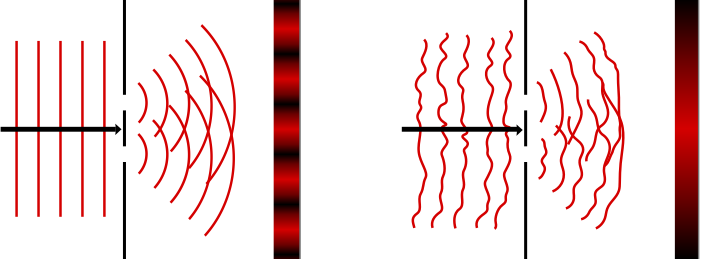
\includegraphics[width=10truecm]{slike/02_Young.pdf}
\caption{Youngov poskus na dveh režah. Le če je vpadno valovanje koherentno, 
se pojavi na zaslonu interferenčni vzorec (levo). Nekoherentno valovanje s spremenljivo
fazo ne da interferenčnega vzorca (desno).}
\label{fig:Young}
\end{figure}

\vglue-5truemm
Svetloba navadnih svetil, na primer plinskih razelektritvenih cevi, 
je zaradi vrste nastanka kaotične narave. 
Atomi v njih sevajo neodvisno, zato se faza izsevanega valovanja neprestano
spreminja. Približno konstantna je le znotraj nekega karakterističnega
časa. Če je pri interferenčnem poskusu karakteristični čas spreminjanja
faze krajši od zakasnitve med valovanjema zaradi različno
dolgih poti, pride na danem mestu zaslona izmenično do konstruktivne in 
destruktivne interference. Čas spreminjanja je praviloma
bistveno krajši od časa opazovanja, zato utripanja ne vidimo in 
zaznamo povprečno razmazano sliko. Interferenčni poskus se ne 
posreči zaradi majhne časovne koherence\index{Koherenca!časovna},
karakterističnemu času spreminjanja faze pa rečemo 
\index{Koherenčni čas}koherenčni čas
$t_{c}$. Časovno koherenco bomo natančneje obravnavali v razdelku
(\ref{sec:casovna-koherenca}), zaenkrat povejmo le, da je časovna
koherenca vezana na fazno razliko med točkami, ki ležijo
vzdolž smeri širjenja valovanja. 

Poleg časovne koherence na interferenčno sliko pomembno vpliva tudi
\index{Koherenca!prostorska}prostorska koherenca, ki je posledica
končne dimenzije svetila. Svetloba, ki na reži vpada iz različnih delov
svetila, ima namreč različno fazo zaradi razlike v dolžini poti 
do rež. Ta faza se prišteje fazni razliki zaradi različno dolgih poti 
od rež do zaslona, zato se interferenčne proge na zaslonu nekoliko 
premaknejo. Če je fazna razlika žarkov iz različnih
delov svetila večja od fazne razlike za režami, se celotna interferenčna
slika na zaslonu izpovpreči. Interferenca se pri Youngovem poskusu
pojavi, kadar sta reži razmaknjeni le toliko, da je povprečna fazna
razlika manjša od $2\pi$. Največjemu prečnemu razmiku, ki še da interferenco,
rečemo prečna koherenčna razdalja\index{Koherenčna razdalja} $d_{c}$. 
Prostorska koherenca, ki jo bomo podrobneje spoznali v razdelku 
(\ref{Prostorska-koherenca}),
je torej vezana na fazno razliko med točkami, ki ležijo prečno 
na smer širjenja valovanja.

Poudarimo še enkrat, da je pojem koherence statističen.
Če je koherenčni čas $t_{c}$ dolg v primerjavi s časom opazovanja,
se seštevajo amplitude valovanj in pojavi se interferenčna slika.
Ta se slučajno spreminja z značilnim časom $t_{c}$. Če pa so razlike
poti večje od $ct_{c}$ ali razmik rež večji od $d_{c}$, gledamo
le povprečno sliko in interferenčne proge izginejo.

\section{Koherenca navadnih svetil}
\label{chap:kns}
Obravnavajmo plinsko razelektritveno cev in z
ustreznim filtrom izberimo eno samo spektralno črto. Ta črta naj ima
osrednjo frekvenco $\nu_{0}$ in končno frekvenčno širino $\Delta\nu$.
Privzamemo, da je glavni prispevek k razširitvi spektralne črte posledica
medatomskih trkov.

Celotna izsevana svetloba je vsota delnih valov, ki izhajajo iz posameznih
atomov in so med seboj neodvisni. Vsak delni val ohranja konstantno fazo
med dvema trkoma, to je v intervalu dolžine $t_{c}$. Valovni paket dolžine 
$t_{c}$ tako vsebuje frekvence v pasu $\Delta \nu$,
za katerega velja $t_{c}\Delta\nu\sim1$. Koherenčni čas je torej
kar reda velikosti obratne vrednosti spektralne širine svetlobe. Povsem
monokromatsko valovanje bi imelo neskončen koherenčni čas in bi bilo
popolnoma koherentno.

Zapišimo še izsevano polje takega svetila. 
Jakost električnega polja v izbrani točki prostora je vsota delnih
valov, ki izvirajo iz raznih delov izvora. Vsak atom v izvoru, naj
jih bo $N$, seva neodvisno, zato so tudi delna valovanja med seboj
neodvisna. Posamična valovanja ohranjajo konstantno fazo v času med
dvema trkoma atoma $t_{c}$. Zaradi enostavnosti privzamemo,
da so amplitude $E_{1}$ in polarizacije izsevanih polj posameznih atomov enake. 
Električno poljsko jakost $E$ v izbrani točki prostora potem 
zapišemo kot vsoto posameznih prispevkov
\begin{equation}
E=E_{1}\sum_{n=1}^{N}e^{i\phi_{n}(t)},
\label{eq:amplituda-random}
\end{equation}
kjer se faza polja $\phi_{n}(t)$, ki ga izseva posamezni atom, naključno
spremeni ob trku z drugim atomom. Povprečje vsote polj je nič, 
povprečni kvadrat skupnega polja, ki je sorazmeren
z gostoto svetlobnega toka, pa je $NE_{1}^{2}$. Zaradi slučajnosti faz je 
slučajna tudi faza celotnega polja in se gotovo povsem spremeni v času, ko se
spremeni faza posameznih prispevkov, to je $t_{c}$. S tako svetlobo bomo videli 
interferenco na režah, če bo razlika poti delnih valovanj manjša od $c\, t_{c}$.

Oglejmo si izračun
na primeru. Imejmo $N=100$ neodvisnih atomov, ki se jim faza naključno
spreminja s karakterističnim časom $t_{c}=10/\nu$, kjer je $\nu$
frekvenca valovanja. Na sliki (\ref{fig:amplituda-intenziteta}) sta
prikazana časovna poteka amplitude $E$ (enačba \ref{eq:amplituda-random})
in $|E|^{2}$.
\begin{figure}
\centering
\def\svgwidth{140truemm} 
\input{slike/02_fluktuacije02.pdf_tex}\\
\def\svgwidth{140truemm} 
\input{slike/02_fluktuacije01.pdf_tex}\\
\def\svgwidth{140truemm} 
\input{slike/02_fluktuacije03.pdf_tex}\\
\def\svgwidth{140truemm} 
\input{slike/02_fluktuacije04.pdf_tex}\\
\caption{Zgoraj: shematski prikaz jakosti električnega polja 
ravnega vala s konstantno fazo (rdeča črta) in jakosti električnega
polja navadnega svetila (modra črta) kot funkcije časa. 
Spodaj: pripadajoča vrednost $|E|^2$ v primeru ravnega vala (rdeča črta) in 
v primeru svetlobe iz navadnega svetila (modra črta) kot funkcija
časa. Modra črtkana črta je povprečna vrednost
$\frac{1}{T}\int_{-T/2}^{T/2}E(t+t')E^{*}(t+t')dt'$
s časom integracije $T=t_{c}$.}
\label{fig:amplituda-intenziteta}
\end{figure}
Za primerjavo je prikazan tudi ravni val\index{Ravni val} $E=\sqrt{N}E_{1}e^{-i\omega t}$
s konstantno fazo in pripadajoč $|E|^{2}$, ki je sorazmeren z gostoto svetlobnega
toka. Ta je v primeru ravnega vala konstantna, medtem ko je povprečna gostota
svetlobnega toka iz navadnega svetila približno konstantna le znotraj $t_{c}$.

\section{Časovna koherenca}
\label{sec:casovna-koherenca}

Časovno koherenco\index{Koherenca!časovna} je najpreprosteje obravnavati 
z \index{Michelsonov interferometer}Michelsonovim 
interferometrom\footnote{Ameriški fizik in nobelovec Albert Abraham Michelson, 1852--1931.},
ki je prikazan na sliki (\ref{fig:michelson}). 
\begin{figure}[!h]
\centering
\def\svgwidth{85truemm} 
\input{slike/02_Michelson.pdf_tex}\\
\caption{\label{fig:michelson}Michelsonov interferometer. Svetlobo
iz izvora $P$ usmerimo skozi kolimacijsko lečo (L) na polprepustno
zrcalo (PZ), s čimer jo razdelimo na dva snopa. S premikanjem 
enega od zrcal (Z) spreminjamo zakasnitev enega delnega snopa in
na detektorju izmenično zaznavamo oslabitve in ojačitve -- opazujemo interferenco.}
\end{figure}

Valovanje iz točke $P$ na polprepustnem zrcalu razdelimo na dva delna snopa, 
nato enega s premikanjem zrcala zakasnimo za $\tau=2x/c$. Dokler je zakasnitev
$\tau$ manjša od koherenčnega časa $t_{c}$, snopa med seboj interferirata.
Ob premikanju zrcala se na detektorju izmenično pojavljajo ojačitve in 
oslabitve. Pri zakasnitvah, ki so večje od koherenčnega časa, ni stalne fazne 
povezave in na detektorju zaznavamo svetlobo, katere intenziteta ni odvisna od lege
zrcala $x$.

\begin{remark}
S kolimacijsko lečo dosežemo, da je čim več žarkov, ki izhajajo iz
$P$, vzporednih z osjo interferometra. V eksperimentih snop svetlobe 
ni nikoli povsem vzporeden in dolžine poti posameznih žarkov se med
seboj malo razlikujejo. Na detektorju tako za $\tau < t_c$ nastanejo jasno 
vidni interferenčni krogi. Pri večjih vrednostih $\tau$  se kontrast interferenčnih
prog zmanjšuje in pri zakasnitvah, ki so daljše od koherenčnega časa, se 
slika povsem zabriše. 
\end{remark}

Zapišimo ugotovitev še matematično.
Gostota svetlobnega toka na detektorju je sorazmerna s kvadratom jakosti električnega
polja obeh delnih valovanj
\begin{equation}
|E_{d}(t)|^{2}=|E(t)+E(t+\tau)|^{2}=|E(t)|^{2}+|E(t+\tau)|^{2}+2\Re \left(E(t)E^{*}(t+\tau)\right).
\label{eq:Michelson-intenziteta}
\end{equation}
Zakasnitev $\tau$ je določena s premikom pomičnega zrcala $\tau=2x/c$.
Navadno opazujemo v času $T$, ki je dolg v primerjavi s koherenčnim
časom svetlobe, zato izraz povprečimo po času
\begin{eqnarray}
\langle|E_{d}(t)|^{2}\rangle & = & \frac{1}{T}\int_{-T/2}^{T/2}|E{}_{d}(t)|^{2}\, dt\nonumber \\
 & = & 2\langle|E(t)|^{2}\rangle+2\Re\langle E(t)E^{*}(t+\tau)\rangle = 2\langle|E(t)|^{2}\rangle+2\Re G(\tau).
 \label{eq:caskohav}
\end{eqnarray}
Prvi člen je vsota povprečnih prispevkov obeh delnih snopov. Privzeli smo, 
da je povprečje polja neodvisno od izbire časovnega intervala.
Drugi člen opisuje interferenco\index{Interferenca}. 
Za opis smo vpeljali
časovno avtokorelacijsko funkcijo\index{Avtokorelacijska funkcija}
jakosti električnega polja 
\boxeq{eq:avtokorelacija}{
G(\tau)=\frac{1}{T}\int_{-T/2}^{T/2}E(t)E^{*}(t+\tau)\, dt.
}
Za zakasnitve $\tau$, ki so krajše od koherenčnega časa $t_c$, je avtokorelacijska
funkcija različna od nič in na
detektorju zaznamo interferenco. Pri zakasnitvah, ki so precej
daljše od koherenčnega časa $t_{c}$, sta polji $E(t)$ in $E(t+\tau)$
statistično neodvisni in povprečje produkta je enako produktu povprečij.
Ker je $\langle E(t)\rangle=0$, pri velikih zakasnitvah $\tau$ interferenčni
člen izgine.

Priročno je vpeljati normirano avtokorelacijsko funkcijo 
\begin{equation}
g(\tau)=\frac{G(\tau)}{G(0)}.
\label{eq:avtokorelacija-norm}
\end{equation}
Za povsem koherentno valovanje je $|g(\tau)|=1$, za povsem nekoherentno
valovanje je $|g(\tau)|=0,$ za delno koherentna  pa $0<|g(\tau)|<1$.
Praviloma se vrednost $|g(\tau)|$ z naraščajočim $\tau$ zmanjšuje,
saj postaja valovanje za velike časovne zamike vedno manj korelirano.
Ohlapno povedano je koherenčni čas zakasnitev, pri kateri postane
vrednost avtokorelacijske funkcije majhna.
Koherenčni čas\index{Koherenčni čas} $t_{c}$ bolj natančno definiramo 
z normirano avtokorelacijsko funkcijo
\boxeq{eq:koherencni-cas}{
t_{c}=\int_{-\infty}^{\infty}\left|g(\tau)\right|^{2}\, d\tau.
}
Zakasnitev delnih valov je pogosto posledica
različno dolgih optičnih poti, zato namesto koherenčnega časa $t_c$
pogosto uporabljamo koherenčno dolžino\index{Koherenčna dolžina} $l_{c}=c\,t_{c}$. 

\begin{definition}
Pokaži, da v navedenih avtokorelacijskih
funkcijah $g(\tau)$ spremenljivka $t_{c}$ ustreza koherenčnemu času,
kot je definiran v enačbi (\ref{eq:koherencni-cas}), in izračunaj $|g(t_{c})|$ za oba primera.
\begin{equation}
g(\tau)=\begin{cases}
\exp\big(i\omega_{0}\tau-\left|\tau\right|/t_{c}\big),\\
\exp\big(i\omega_{0}\tau-\pi\tau^{2}/2t_{c}^{2}\big),
\end{cases}
\label{eq:gauss-eksponent}
\end{equation}

Ob nalogi (\ref{naloga-spekter}) in v razdelku~(\ref{Razsiritev}) 
bomo spoznali, da sta to avtokorelacijski
funkciji za svetlobo z \index{Spekter!Lorentzov}Lorentzovim spektrom
(razširitev spektralne črte zaradi medatomskih trkov) in Gaussovim spektrom\index{Spekter!Gaussov}
(Dopplerjeva razširitev)\index{Dopplerjeva razširitev}.
\end{definition}

Poglejmo nekaj značilnih vrednosti koherenčnih dolžin. 
Koherenčna dolžina svetlobe, izsevane iz črnega telesa, je $l_{c}=c\,t_{c}\approx 
\hbar c/k_{B}T$ (glej nalogo~\ref{naloga-Planck})\index{Sevanje črnega telesa}. 
Svetloba s Sonca ($T \approx 6000$~K)
ima tako koherenčno dolžino zgolj $\sim 0,4~\si{\micro\metre}$, kar ustreza
koherenčnemu času $t_c \sim 1~\si{fs}$. Svetloba,
izsevana iz LED sijalk\index{LED}, ima koherenčno dolžino $\sim20$--$100~\si{\micro\metre}$.
Živosrebrna svetilka ima za izbrano spektralno črto koherenčno dolžino
do okoli $50~\si{\centi\metre}$, kar ustreza koherenčnemu času $t_c \sim 1,6~\si{ns}$.
Koherenčna dolžina svetlobe, izsevane iz laserjev, je tipično okoli $100~\si{\metre}$, 
v nekaterih vlakenskih laserjih\index{Laser!vlakenski} pa koherenčna dolžina 
presega $100~\si{\kilo\metre}$.

\section{Zveza med avtokorelacijsko funkcijo in spektrom}

Obravnavajmo zdaj koherenco poljubnega valovanja, ki
je v povprečju stacionarno. To pomeni, da se povprečna gostota svetlobnega
toka v času zajemanja, ki traja čas $T$, ne spreminja in da je avtokorelacijska funkcija
odvisna le od $\tau$. Vzorec valovanja razvijemo
v Fourierevo vrsto
\begin{equation}
E(t)=\sum_{n}A_{n}(\omega)e^{-i n \Delta\omega t},\mbox{\hskip1cm}\Delta\omega=\frac{2\pi}{T}.
\end{equation}
Amplitude $A_{n}(\omega)$ so slučajne spremenljivke, ki predstavljajo delež polja pri 
krožni frekvenci $\omega=n\Delta\omega$, čas opazovanja $T$ pa naj bo bistveno daljši od $t_{c}$. 
Potem zapišemo amplitude $A_n$
\begin{equation}
A_{n}(\omega)=\frac{1}{T}\int_{-T/2}^{T/2}E(t)\, e^{i\omega t}\, dt.\label{eq:amplituda-An}
\end{equation}
Kvadrat $|A_{n}(\omega)|^{2}$ je sorazmeren z gostoto svetlobnega toka pri krožni
frekvenci $\omega$ in predstavlja intenziteto\index{Intenziteta}
valovanja\footnote{Intenziteto valovanja na splošno vpeljemo kot $I = |E|^2$, gostota svetlobnega
toka pa je $j = \varepsilon \varepsilon_0 c |E|^2/2$ z enotami W/m$^2$ (enačba~\ref{eq:jcw}). 
Kadar predfaktorji niso pomembni, pogosto uporabljamo krajši izraz.}. 
Intenziteto svetlobe pri $\omega$, deljeno z intervalom $\Delta\omega$, imenujemo  
\index{Spekter}spekter $S(\omega)$
\begin{equation}
S(\omega)=\frac{|A_{n}(\omega)|^{2}}{\Delta\omega}=\frac{T}{2\pi}|A_{n}(\omega)|^{2}.
\end{equation}
Vstavimo še amplitudo $A_{n}$ (enačba \ref{eq:amplituda-An}) in dobimo 
\begin{equation}
S(\omega) =\frac{1}{2\pi T}\int\int_{-T/2}^{T/2}E(t)E^{*}(t^{\prime})\, 
e^{-i\omega(t^{\prime}-t)}\, dt\, dt^{\prime}.
\end{equation}
Uvedemo novo spremenljivko $\tau=t^{\prime}-t$ in zapišemo
\begin{equation}
S(\omega)=\frac{1}{2\pi T}\int_{-\infty}^{\infty}e^{-i\omega\tau}d\tau\int_{-T/2}^{T/2}E(t)E^{*}(t+\tau)\, dt.
\label{eq:spekter}
\end{equation}
Integral po $t$ je ravno enak korelacijski funkciji $G(\tau)$ 
(enačba~\ref{eq:avtokorelacija}). Privzeli smo, da velja $T\gg t_{c}$, zato 
je korelacijska funkcija na mejah integracije po $\tau$ praktično enaka nič in 
meje integracije smo lahko raztegnili do neskončnosti. Zveza, ki smo jo dobili, je 
\index{Wiener-Hinčinov izrek} 
Wiener-Hinčinov izrek\footnote{Ameriški matematik Norbert Wiener, 1894--1964, in 
ruski matematik Aleksander Jakovljevič Hinčin, 1894--1959.}
\boxeq{eq:spekter-zveza}{
S(\omega)=\frac{1}{2\pi}\int_{-\infty}^{\infty}G(\tau)e^{-i\omega\tau}\, 
d\tau\;\Longleftrightarrow\; G(\tau)=\int_{-\infty}^{\infty}S(\omega)e^{i\omega\tau}\, 
d\omega.
}
Spekter v povprečju stacionarne svetlobe je torej Fouriereva transformiranka 
avtokorelacijske funkcije svetlobnega polja. 

Vendar je spekter, ki smo ga zapisali z enačbo~(\ref{eq:spekter}), zapisan za izbran 
vzorec valovanja, ki traja čas $T$, in je tudi slučajna spremenljivka. Če je proces
nestacionaren, moramo izrek preoblikovati, tako da namesto količin $S$ in $G$ zapišemo
povprečne količine. Povprečni spekter dobimo tako, da naredimo
limito $T \rightarrow \infty$. 
\begin{equation}
\langle S (\omega) \rangle = \lim_{T\to \infty}S(\omega).
\end{equation}
Za povprečni spekter velja, da je enak Fourierevi transformiranki 
povprečne avtokorelacijske funkcije svetlobnega polja.

Iz Wiener-Hinčinovega izreka (enačba~\ref{eq:spekter-zveza}) neposredno sledi, da je 
koherenca nekega valovanja tesno povezana z njegovim spektrom in 
koherenčni čas $t_{c}$ povezan s spektralno 
širino svetlobe $\gamma$. Velja (glej nalogo~\ref{naloga:gammatc})\index{Koherenčni čas}
\boxeq{eq:spektralna-sirina-zveza}{
\gamma=\frac{1}{t_{c}}.
}
Valovanje z dolgim $t_c$ ima zelo majhno spektralno širino (ozek spekter), 
valovanje s kratkim $t_c$ pa ima širok spekter. To je v skladu s primeri, navedenimi na koncu
prejšnjega razdelka: svetloba s Sonca ima širok spekter in zelo kratek koherenčni čas, 
svetloba iz laserjev pa ima praviloma ozko spektralno črto in dolg koherenčni čas. Ugotovimo 
tudi, da lahko valovanju z ustreznim spektralnim filtriranjem podaljšamo koherenčni čas.
\begin{definition}
\label{naloga:gammatc}
Formalno vpeljemo spektralno širino kot 
\begin{equation}
\gamma=\frac{1}{2\pi\int_{-\infty}^{\infty}\left|s(\omega)\right|^{2}\, d\omega}; \quad
\mathrm{kjer~je} \quad
s(\omega)=\frac{S(\omega)}{\int_{-\infty}^{\infty}S(\omega) d\omega} =\frac{S(\omega)}{G(0)}
\label{eq:spektralna-sirina}
\end{equation}
normirani spekter. 
Z uporabo enačbe za koherenčni čas $t_{c}$ (enačba \ref{eq:koherencni-cas})
pokaži, da je spektralna širina obratno sorazmerna s koherenčnim
časom (enačba \ref{eq:spektralna-sirina-zveza}) ne glede na
obliko spektra. \\
Namig: Uporabi Parsevalov izrek, ki pravi:
\begin{equation}
\int_{-\infty}^{\infty}\left|f(t)\right|^{2}\, dt={2\pi}
\int_{-\infty}^{\infty}\left|F(\omega)\right|^{2}\, d\omega,
\end{equation}
kjer je 
\beq
F(\omega)=\frac{1}{2\pi} \int_{-\infty}^{\infty}f(t)e^{-i\omega\tau}\, d\tau
\eeq
Fouriereva transformiranka funkcije $f(t)$.
\end{definition}

Za zgled Wiener-Hinčinovega izreka vzemimo primer, ki je predstavljen na 
sliki~(\ref{fig:amplituda-intenziteta}). 
Ker so trki med atomi naključni, je avtokorelacijska funkcija eksponentno pojemajoča
\beq
g(\tau)=e^{i\omega_{0}\tau} e^{-\tau/t_{c}}.
\label{eq:g-primer}
\eeq
Vemo, da je spekter take svetlobe Lorentzove 
oblike\index{Spekter!Lorentzov} (glej nalogo~\ref{naloga-spekter})
\begin{equation}
s(\omega)=\frac{1}{\pi}\frac{\gamma}{(\omega-\omega_{0})^{2}+\gamma^{2}},
\label{eq:spekter-primer}
\end{equation}
pri čemer je $\gamma=1/t_{c}$ spektralna širina. 
Normirani spekter $s(\omega)$ in ustrezna avtokorelacijska funkcija $g(\tau)$ 
sta prikazana na sliki~(\ref{fig:SpekterAc}). 
Točke na grafih 
predstavljajo spekter in izračunano avtokorelacijsko funkcijo 
za integracijski čas $T=100\,t_{c}$. Za primerjavo sta z rdečo 
krivuljo prikazana tudi pričakovani spekter (enačba~\ref{eq:spekter-primer}) in avtokorelacijska
funkcija (enačba~\ref{eq:g-primer}). Zaradi končnega
časa $T$ pri izračunu povprečja se spekter iz simulacije nekoliko razlikuje
od pričakovanega. 
\begin{figure}[h]
\centering
\def\svgwidth{65truemm} 
\input{slike/02_spekter.pdf_tex}\qquad
\def\svgwidth{65truemm} 
\input{slike/02_avtokorelacija.pdf_tex}
\caption{Spekter in avtokorelacijska funkcija valovanja s slike~(\ref{fig:amplituda-intenziteta})}
\label{fig:SpekterAc}
\end{figure}

\begin{definition}
\label{naloga-spekter}
Imejmo dve vrsti svetlobe. Prva naj ima avtokorelacijsko funkcijo, ki je eksponentno pojemajoča, druga
pa ima avtokorelacijsko funkcijo Gaussove oblike (enačbi~\ref{eq:gauss-eksponent}). Pokaži, da sta njuna
spektra oblike\index{Spekter!Gaussov}\index{Spekter!Lorentzov}
\begin{equation}
s(\omega)=
\frac{1}{\pi}\frac{\gamma}{(\omega-\omega_{0})^{2}+\gamma^{2}} \quad \mathrm{in} \quad 
s(\omega)= \frac{1}{\sqrt{2}\pi\gamma}\exp\big(-
\frac{\left(\omega-\omega_{0}\right)^{2}}{2\pi\gamma^{2}}\big),
\end{equation}
kjer je $\gamma=1/t_{c}$ spektralna širina. 
\end{definition}

Spektralne črte atomov so pogosto Lorentzove oblike, kar je posledica
eksponentnega razpada stanj (naravna širina). Dodatno se spektralne
črte razširijo zaradi trkov med atomi, vendar tudi to vodi do približno Lorentzove
oblike spektra. V plinih je pogosto prevladujoča razširitev črt
zaradi Dopplerjevega pojava (glej razdelek~\ref{Razsiritev}). Spekter 
Dopplerjevo razširjene svetlobe je Gaussove oblike in iz enačbe~(\ref{eq:spekter-zveza})
sledi, da je v tem primeru tudi avtokorelacijska funkcija Gaussove oblike.
\vglue1truecm

\begin{definition}\label{naloga-Planck}
Numerično pokaži, da je koherenčni čas svetlobe, ki jo oddaja črno telo s 
temperaturo $T$, približno enak $t_{c}\approx{\hbar}/{k_{B}T}$.\index{Sevanje črnega telesa}
Normirani spekter sevanja črnega telesa zapišemo 
kot \index{Spekter!Planckov}Planckov spekter 
\begin{equation}
s(\omega)=\frac{15}{\pi^{4}} \frac{\hbar^4\omega^3}{(kT)^4}/\left(e^{\hbar\omega/kT}-1\right)
\quad \textrm{za}~\omega >0,~\textrm{sicer}~s(\omega) = 0.
\label{eq:Planckov-spekter}
\end{equation}
\end{definition}

\begin{remark}\index{Fouriereva spektroskopija}
V prejšnjem razdelku smo spoznali, da časovno avtokorelacijsko funkcijo
merimo z Michelsonovim interferometrom. Dobljena povezava med merjeno
avtokorelacijo in izračunanim spektrom je osnova za Fourierevo 
spektroskopijo,
pri kateri določimo absorpcijski ali emisijski spekter
snovi iz izmerjene avtokorelacijske funkcije. Tak pristop
ima nekatere pomembne prednosti pred drugimi metodami in se danes
precej uporablja, posebej v infrardečem delu EM valovanja (tako imenovana
metoda FTIR - {\it Fourier-transform infrared spectroscopy}).\index{Infrardeče valovanje}\index{FTIR}
\end{remark}

\section{Prostorska koherenca}
\label{Prostorska-koherenca}
\index{Koherenca!prostorska}
Vrnimo se k Youngovemu poskusu\index{Youngov poskus} in interferenci
\index{Interferenca} na dveh ozkih režah. Osvetljujmo zdaj zaslon, v katerem sta dve odprtini,
s svetilom končnih razsežnosti. Svetilo naj sveti skoraj enobarvno
svetlobo in naj bo na simetrali med odprtinama, kot kaže slika~(\ref{fig:shema-interferenca}).

Žarka, ki izhajata iz sredine svetila (polna rdeča črta), 
opravita do odprtin v ravnini A enako dolgo pot in povzročita na zaslonu B 
interferenčne proge. Žarka, ki izhajata z roba izvora (prekinjena rdeča črta), 
imata do odprtin različno dolgo pot, zato nastane med njima fazna razlika že do ravnine A, 
ki se prišteje fazni razliki do ravnine B. Interferenčne proge, ki jih tvorita 
robna žarka, so premaknjene glede na proge sredinskih žarkov. Ker so žarki z roba
statistično neodvisni od žarkov iz sredine, z njimi
ne interferirajo. Celotni interferenčni vzorec je zato kar vsota interferenčnih
vzorcev žarkov iz različnih delov svetila. Če je razlika poti za žarke
iz različnih delov velikosti valovne dolžine $\lambda$, se celotna
interferenčna slika na zaslonu B izpovpreči.

\begin{figure}[h]
\centering
\def\svgwidth{140truemm} 
\input{slike/02_precnaKoherenca.pdf_tex}
\caption{Shema interferenčnega eksperimenta z razsežnim svetilom}
\label{fig:shema-interferenca}
\end{figure}

Razdaljo med odprtinama, pri kateri interferenčne proge
izginejo, imenujemo\index{Koherenčna razdalja} prečna koherenčna razdalja $d_c$. 
Zanjo velja približno 
\begin{equation}
\delta s = d_c\sin\varphi\approx d_c\frac{R}{z}\sim\lambda\;\Rightarrow\;
d_{c}\sim\frac{z\lambda}{R}.
\label{eq:prost_koh}
\end{equation}
\begin{remark}
Pogosto je v uporabi
pojem \index{Koherenčna ploskev}koherenčna ploskev, to je območje, 
v katerem je fazna razlika v povprečju konstantna. Velikost te ploskve je približno $d_{c}^{2}$.
V območju koherenčne ploskve so tudi valovne fronte približno gladke.
Vsekakor moramo paziti, da koherenčne razdalje $d_c$ ne zamenjamo
s koherenčno dolžino $l_c$, ki smo jo vpeljali pri časovni koherenci valovanja. 
\end{remark}

Zapišimo gornje ugotovitve nekoliko bolj natančno. Na zaslonu $B$
izmerimo povprečno gostoto svetlobnega toka, ki je sorazmerna povprečju kvadrata
jakosti električnega polja. To je sestavljeno iz valovanj iz obeh odprtin
\begin{align}
\langle|E|^{2}\rangle & =\langle|K_{1}E_{1}+K_{2}E_{2}|^{2}\rangle\nonumber \\
&=  |K_{1}|^{2}\langle|E_{1}|^{2}\rangle+|K_{2}|^{2}\langle|E_{2}|^{2}\rangle+
2\Re \left( K_{1}K_{2}^{*}\langle E_{1}(t)E_{2}^{*}(t+\tau)\rangle\right).
\end{align}
Pri tem je $\tau=d\sin\vartheta/c$ zakasnitev valovanja iz druge odprtine
glede na valovanje iz prve, faktorja $K_{1}$ in $K_{2}$ pa sta določena
z uklonom na posameznih odprtinah. Interferenčna slika je vsebovana v podobnem 
členu kot pri Michelsonovem interferometru (enačba~\ref{eq:caskohav}), 
le da nastopa v tem primeru namesto avtokorelacijske funkcije
navzkrižna korelacijska funkcija polj $E_{1}$ in $E_{2}$ iz obeh 
odprtin.\index{Navzkrižna korelacijska funkcija} 

Kako je interferenčni člen povezan z lastnostmi svetila, brez težav
doženemo v izbranem primeru skoraj enobarvne svetlobe z osrednjo krožno frekvenco
$\omega$. Tedaj lahko za zakasnitve $\tau$, ki so krajše
od koherenčnega časa, zapišemo 
\begin{equation}
E_{2}(\tau)=E_{2}(0)\, e^{-i\omega\tau}
\end{equation}
 in 
\begin{equation}
\langle E_{1}(t)E_{2}^{*}(t+\tau)\rangle=
\langle E_{1}(t)E_{2}^{*}(t)\rangle 
e^{i\omega\tau}=J(P_{1},P_{2})\, e^{i\omega\tau}.
\end{equation}
Faktor $\Re e^{i\omega\tau}= \cos(\omega \tau) = \cos(kd\sin\vartheta)$ da interferenčne
proge za koherentno osvetlitev zaslona, povprečje produkta polj
v odprtinah ob istem času $J(P_{1},P_{2})=\langle E(P_{1},t)E^{*}(P_{2},t)\rangle$
pa meri stopnjo prečne koherence med obema odprtinama. Od velikosti
tega člena je odvisen kontrast interferenčnih prog. Izračunajmo ga.

Polje v posamezni odprtini je vsota prispevkov iz celega izvora.
\begin{equation}
E(P_{j})=-\frac{i}{\lambda}\int E(\xi,\eta)\frac{e^{iks_{j}}}{s_{j}}\, d\xi\, d\eta.
\end{equation}
Pri tem je $s_{j}$ razdalja med točko na izvoru s koordinato $(\xi,\eta)$  in točko
$P_{j}(x_{j},y_{j})$ v odprtini na ravnini A (glej sliko \ref{fig:shema-interferenca}).
Faktor pred integralom $-i/\lambda$ izhaja iz uklonske teorije (enačba~\ref{eq:Fresnel-Kirchoffov-integral}).
Tako je 
\begin{equation}
J(P_{1},P_{2})=\frac{1}{\lambda^{2}}\int\int\langle E(\xi,\eta)E^{*}(\xi^{\prime},\eta^{\prime})\rangle\frac{e^{ik(s_{1}-s_{2}^{\prime})}}{s_{1}s_{2}^{\prime}}\, d\xi\, d\eta\, d\xi^{\prime}d\eta^{\prime}.\label{eq:field-correlation}
\end{equation}
V izbranem svetilu sevajo atomi neodvisno. Valovanji iz dveh točk svetila,
ki sta razmaknjeni za več kot $\lambda$, sta neodvisni in povprečje
njunega produkta je enako nič. Tako približno velja 
\begin{equation}
\langle E(\xi,\eta)E^{*}(\xi^{\prime},\eta^{\prime})\rangle=\frac{\lambda^{2}}{\pi} \cdot \delta(\xi-\xi^{\prime},\eta-\eta^{\prime})\langle|E(\xi,\eta)|^{2}\rangle.
\label{eq:delta-Zernike}
\end{equation}
Faktor $\lambda^{2}/\pi$ poskrbi za ustrezno normalizacijo. 
Naj bo oddaljenost svetila od zaslona $A$
veliko večja od dimenzije svetila ($z\gg R$), tako da lahko imenovalec pod integralom
v izrazu~(\ref{eq:field-correlation}) nadomestimo z $z^{2}$ in postavimo
pred integral. Sledi
\begin{equation}
J(P_{1},P_{2})=\frac{1}{\pi z^{2}}\int\langle|E(\xi,\eta)|^{2}\rangle e^{ik(s_{1}-s_{2})}\, d\xi\, d\eta.\label{eq:Zernike1}
\end{equation}
Izraz lahko še nekoliko poenostavimo, če razvijemo $s_{1}$
in $s_{2}$ 
\begin{equation}
s_{j}=\sqrt{z^{2}+(x_{j}-\xi)^{2}+(y_{j}-\eta)^{2}}\approx z+\frac{(x_{j}-\xi)^{2}+(y_{j}-\eta)^{2}}{2z}.
\end{equation}
Pišemo še $\langle|E(\xi,\eta)|^{2}\rangle=I(\xi,\eta)$ ter $x_{2}-x_{1}=\Delta x$
in $y_{2}-y_{1}=\Delta y$. S tem dobimo tako imenovani \index{van Cittert-Zernikov izrek}
van Cittert-Zernikov izrek\footnote{Nizozemski fizik Pieter Hendrik van Cittert, 1889--1959, in 
nizozemski fizik in nobelovec Frits Zernike, 1888--1966.}
\boxeq{eq:Zernike2}{
J(\Delta x,\Delta y)=\frac{e^{-i\phi}}{\pi z^{2}}\int I(\xi,\eta)e^{ik(\Delta 
x\xi+\Delta y\eta)/z}\, d\xi\, d\eta.
}

Faza 
\begin{equation}
\phi=\frac{\pi}{\lambda z}[(x_{2}^{2}+y_{2}^{2})-(x_{1}^{2}+y_{1}^{2})]
\end{equation}
meri skupni premik interferenčnih prog, do katerega pride, kadar svetilo
ne leži na isti osi kot odprtini v zaslonu. Kadar ležita odprtini v ravnini $A$ 
simetrično glede na os svetila, je faza $\phi$ enaka nič.

Dobljeni rezultat si je vredno nekoliko ogledati. Prečno prostorsko
korelacijsko funkcijo $J(P_{1},P_{2})$, ki določa kontrast interferenčnih
prog na zaslonu, smo izrazili kot 2-D  Fourierevo transformiranko intenzitete svetlobe
na samem svetilu (enačba \ref{eq:Zernike2}). 
\begin{remark}
Ob tem se spomnimo,
da velja podobna zveza med jakostjo električnega polja v osvetljeni odprtini 
in njeno Fraunhoferjevo uklonsko sliko (enačba~\ref{eq:FraunhoferApprox}), 
pri čemer so količine, ki nastopajo v obeh zvezah,
povsem različne. Različna je tudi veljavnost obeh izrazov: medtem ko je Fraunhoferjeva
uklonska formula veljavna le v veliki oddaljenosti, za opis uklonske slike v bližnjem polju
pa je treba uporabiti Fresnelov izraz (enačba~\ref{eq:FresnelApprox}), 
je rezultat za $J(P_{1},P_{2})$ (enačba~\ref{eq:Zernike2}) veljaven v obeh območjih.\index{Fraunhoferjev uklon}
\index{Fresnelov uklon}
\end{remark}

Pri velikih razdaljah med točkama $P_{1}$ in $P_{2}$ vrednost $J(P_{1},P_{2})$ 
gotovo pade na nič. Največja razdalja, do katere je $J(P_{1},P_{2})$ še različna od nič, je ravno
prečna koherenčna razdalja $d_{c}$, ustrezna ploskev pa je koherenčna
ploskev $S_{c}$\index{Koherenčna ploskev}. Iz izraza za koherenčno razdaljo 
(enačba \ref{eq:prost_koh}) jo lahko ocenimo
\begin{equation}
S_{c}\sim\frac{(\lambda z)^{2}}{S_{0}}\sim\frac{\lambda^{2}}{\Omega_{0}},
\label{eq:koherencna-ploskev}
\end{equation}
kjer je $S_{0}$ površina svetila, $\Omega_{0}$ pa prostorski kot,
pod katerim je videti svetilo v ravnini $A$. 

Oglejmo si primer. Naj bo svetilo v obliki kroga 
s polmerom $R$, obe odprtini v zaslonu naj imata koordinati $x$ enaki nič, razmik
med njima v smeri $y$ pa naj bo $d$. 
Prečno korelacijsko funkcijo izračunamo iz enačbe~(\ref{eq:Zernike2}) in dobimo 
(glej nalogo~\ref{naloga:J})
\begin{equation}
J(0,d)=2\frac{R^{2}I_{0}}{z^{2}}\,\frac{J_{1}(kRd/z)}{kRd/z},
\label{eq:jkrozna}
\end{equation}
kjer je $J_{1}(x)$ Besslova funkcija. V ničlah prve Besslove funkcije
pade prečna korelacijska funkcija $J$ na nič in interferenčnega vzorca ne vidimo. 
Za določitev prečne koherenčne razdalje je zato smiselno vzeti ravno prvo ničlo Besslove funkcije
$J_1$, to je pri
\beq
\label{eq:okroglo_svetilo}
d_{c} \approx 3,83 \frac{z}{kR} = 0,61 \frac{\lambda z}{R}.
\eeq
\begin{definition}
\label{naloga:J}
Pokaži, da prečno korelacijsko funkcijo za okroglo svetilo s polmerom $R$, pri čemer
odprtini na zaslonu ležita simetrično na osi $y$ v razmiku $d$, zapišemo z enačbo~(\ref{eq:jkrozna}). 
\end{definition}

Doslej smo obravnavali le valovanje v središču interferenčne slike na
zaslonu $B$, to je pri tako majhnih kotih $\vartheta$, da je zakasnitev
manjša od koherenčnega časa. Pri večjih kotih moramo upoštevati še
vpliv končnega koherenčnega časa, zaradi česar se kontrast interferenčnih
prog še dodatno zmanjšuje. Interferenčna slika je 
tako produkt časovnega in prostorskega dela. 

Poglejmo še primer dveh zelo tankih vzporednih rež. 
Za nekaj različnih razmikov med režama $d$ je intenziteta
svetlobe na zaslonu prikazana na sliki~(\ref{fig:Interferencna-slika}).
Če je $d\ll\lambda z/R$ (a), je modulacija interferenčnih prog v sredini
popolna in se zaradi končnega koherenčnega časa zmanjšuje le pri večjih
kotih $\vartheta$. Pri nekaj večjem razmiku (b) tudi v sredini kontrast
ni več popoln. Obenem se interferenčne proge zgostijo. Kadar je $d\approx 3,83\,z/kR$,
dosežemo prvo ničlo Besslove funkcije $J_{1}(x)$ in interferenčni vzorec
prvič izgine (c). Takrat je razdalja med režama ravno enaka prečni
koherenčni razdalji valovanja. Pri še večjih razmikih (d) 
je Besslova funkcija negativna in ponovno se pojavijo interferenčne proge, 
vendar so slabše izražene in z nasprotno fazo, kar da v sredini temno progo. 
\index{Interferenca}

\begin{figure}[h]
\begin{center}
\def\svgwidth{0.37\textwidth} 
\input{slike/02_interferenca01.pdf_tex}
\def\svgwidth{0.37\textwidth} 
\input{slike/02_interferenca02.pdf_tex}
\def\svgwidth{0.37\textwidth} 
\input{slike/02_interferenca03.pdf_tex}
\def\svgwidth{0.37\textwidth} 
\input{slike/02_interferenca04.pdf_tex}
\caption{Interferenčna slika na zaslonu
za različne vrednosti razmikov med režama: (a) $d = z/kR$, (b) $d=2z/kR$, 
(c) $d = 3,832\,z/kR$ in (d) $d = 5,136\,z/kR$. 
Z večanjem razdalje med režama se proge zgostijo in kontrast se zmanjša. Koherenčni
čas svetlobe je $t_{c}=10/\omega$, kar še dodatno zmanjšuje modulacijo
interferenčnih prog. Pri $d=3,832\,z/kR$ je prva ničla Besslove
funkcije in interferenčni vzorec popolnoma izgine. Pri večjih $d$ so interferenčne
proge spet vidne, vendar z manjšim kontrastom in nasprotno fazo.}
\label{fig:Interferencna-slika}
\end{center}
\end{figure}

\begin{remark}
Merjenje prečne koherenčne razdalje svetlobe iz
zvezd je osnova za Michelsonovo metodo določanja zvezdnih premerov.
Svetlobo iz izbrane zvezde zberejo v teleskop preko dveh manjših parov
zrcal, kjer sta zunanji zrcali na pomičnih rokah, tako da ju je mogoče
razmikati. Glavno zrcalo teleskopa zbere svetlobna snopa v goriščni
ravnini, kjer nastanejo interferenčne proge, če le pomični zrcali
nista preveč razmaknjeni. Iz razmika, pri katerem interferenčne proge
izginejo, je mogoče določiti premere bližnjih svetlih zvezd. Za zvezdo
s polmerom $10^{6}$ km v razdalji 5 svetlobnih let je prečna koherenčna
razdalja za zeleno svetlobo okoli $15$~m, kar je z Michelsonovim
zvezdnim interferometrom mogoče izmeriti. Pri zvezdah, ki so dlje
od nekaj deset svetlobnih let, metoda odpove.
\end{remark}


%Končano

%-------------------------------------------------------------------------------
%	CHAPTER 3
%-------------------------------------------------------------------------------

\chapterimage{slike/Laguerre.jpg} % Chapter heading image

\chapter{Koherentni snopi svetlobe}
V tem poglavju bomo zapisali obosni približek valovne enačbe in spoznali 
njeno osnovno rešitev: Gaussov snop. Obravnavali bomo snope osnovnega in višjega reda ter
se naučili računati prehode Gaussovih snopov prek optičnih elementov. 

\section{Omejen snop svetlobe}
Pri obravnavi elektromagnetnega valovanja pogosto uporabljamo
približek ravnih valov\index{Ravni val}. Ti so v smeri pravokotno na smer širjenja
neomejeni in so zato lahko le idealizacija. Čim raven val usmerimo skozi odprtino
v zaslonu, nastane omejen snop svetlobe\index{Omejen snop}. V snopu svetlobe valovna čela niso
ravna in meje snopa niso vzporedne, ampak se snop zaradi uklona širi\index{Uklon} 
(slika \ref{fig:Uklon-na-rezi}).
\begin{figure}[h]
\centering
\def\svgwidth{120truemm} 
\input{slike/03_uklon_na_rezi.pdf_tex}
\caption{Omejen snop nastane ob prehodu ravnega vala skozi končno odprtino.}
\label{fig:Uklon-na-rezi}
\end{figure}

V veliki oddaljenosti od zaslona lahko za izračun polja uporabimo
\index{Fraunhoferjev uklon}Fraunhoferjevo uklonsko teorijo (glej poglavje~\ref{FFuklon}). 
Vendar za oceno kota širjenja podrobnega računa niti ne potrebujemo. Velja približno 
\begin{equation}
\vartheta\sim\frac{\lambda}{a},
\label{eq:kot_ocena}
\end{equation}
kjer je $a$ polmer odprtine v zaslonu.
Opis polja v bližini zaslona je zahtevnejši, saj je treba uporabiti 
Fresnelov približek\index{Fresnelov uklon}. S slike (\ref{fig:Uklon-na-rezi})
ocenimo, da velja
\begin{equation}
\frac{a}{b}\sim{\vartheta}\sim \frac{\lambda}{a} \qquad \mathrm{in~tako} \qquad b\sim\frac{a^2}{\lambda}.
\label{eq:z_ocena}
\end{equation}

Včasih taki približni oceni zadoščata. Bolj kvantitativen opis omejenih
snopov bi lahko dobili s Fraunhoferjevo in Fresnelovo uklonsko teorijo,
kar pa ni najudobnejša pot. Lotimo se naloge raje preko približka
obosne valovne enačbe.

\begin{definition}
Pokaži, da je Fraunhoferjeva uklonska slika reže, katere prepustnost se v radialni smeri
spreminja kot Gaussova funkcija $T(\xi, \eta)=e^{-(\xi^2+\eta^2)/w_0^2}$, podana z Gaussovo funkcijo
oblike $E(x,y,z) \propto e^{-(x^2+y^2)/w^2(z)}$ in določi odvisnost $w(z)$. Izračunaj še 
uklonsko sliko v bližnjem polju po Fresnelovi uklonski teoriji.
\end{definition}

\section{Obosna valovna enačba}
Pričnimo s časovno neodvisno valovno enačbo za monokromatsko valovanje
s frekvenco $\omega$, to je \index{Helmholtzeva enačba}Helmholtzevo enačbo (enačba~\ref{eq:Helmholtz})
\begin{equation}
\nabla^{2}E+k^{2}E=0,
\label{eq:valovna-enacba-hh}
\end{equation}
kjer je $k=n\omega/c_{0}$ valovno število in $n$ lomni količnik
sredstva, po katerem se valovanje širi. Zaradi enostavnosti obravnavajmo
le eno polarizacijo, tako da $E$ pišemo kot skalar. Iščemo rešitev za
omejen snop, ki se širi približno vzdolž osi $z$. Zapišimo jo v obliki
\begin{equation}
E=E_{0}\psi(\mathbf{r},z)e^{ikz},
\label{eq:ravni-val-nastavek}
\end{equation}
kjer je $\mathbf{r}$ krajevni vektor v ravnini $xy$. Glavni del odvisnosti
od koordinate $z$ smo zapisali v faktorju $e^{ikz}$, tako da lahko
privzamemo, da se $\psi$ v smeri $z$ le počasi spreminja. Vstavimo
gornji nastavek v Helmholtzevo enačbo (enačba~\ref{eq:valovna-enacba-hh})
in pri tem zanemarimo druge odvode po $z$, saj je zaradi počasnega spreminjanja
$\partial^{2}\psi/\partial z^{2}$ majhen v primerjavi s $k\partial\psi/\partial z$ in $k^{2}\psi$.
Zaenkrat obravnavajmo le radialno simetrične rešitve. Dobimo obosno
ali paraksialno valovno enačbo\index{Obosna valovna enačba}
\index{Paraksialna enačba|see{Obosna valovna enačba}}
\boxeq{eq:obosna-valovna-enacba}{
\nabla_{\perp}^{2}\psi=-2ik{\frac{{\partial\psi}}{{\partial z}}}.
}
\begin{remark} 
Opazimo, da je obosna valovna enačba enaka Schr\"{o}dingerjevi enačbi
za prost delec v dveh dimenzijah, v kateri ima koordinata $z$ vlogo
časa. Omejenemu snopu v kvantni mehaniki ustreza lokaliziran delec
-- valovni paket. Ta se s časom širi, kar v optiki ustreza pojavu uklona.
\end{remark}
Zapišimo nastavek za ravni val \index{Ravni val} v obliki
\begin{equation}
\psi=e^{ik_{1}x+ik_{2}y}\, e^{-i\beta z}.
\label{eq:ravni-val-nastavek-obosni}
\end{equation}
Da bo gornji nastavek rešitev
obosne valovne enačbe~(enačba~\ref{eq:obosna-valovna-enacba}), mora veljati 
\begin{equation}
\beta=\frac{k_{1}^{2}+k_{2}^{2}}{2k}.
\end{equation}
Ko vstavimo nastavek za $\psi$ v izraz za polje $E$ 
(enačba~\ref{eq:ravni-val-nastavek}), dobimo ravni val, za katerega velja 
\begin{equation}
k_{3}=k-\beta=k-\frac{k_{1}^{2}+k_{2}^{2}}{2k},\label{eq:k3-razvoj}
\end{equation}
 pri čemer je $k_{3}$ vzdolžna in $k_{1}$ ter
$k_{2}$ prečni komponenti valovnega vektorja, $k$ pa valovno število. 
Za ravni val, ki je rešitev valovne enačbe (enačba~\ref{eq:valovna-enacba-hh})
in ne obosnega približka, velja 
\begin{equation}
k_{3}=\sqrt{k^{2}-(k_{1}^{2}+k_{2}^{2})}.\label{eq:k3-tocno}
\end{equation}
Očitno dobimo enačbo~(\ref{eq:k3-razvoj}) iz enačbe~(\ref{eq:k3-tocno})
z razvojem za majhne vrednosti $k_1$ in $k_2$. To pove, da je približek obosne 
enačbe dober, kadar je razmerje prečne in vzdolžne komponente valovnega vektorja 
majhno. Takrat je majhen tudi kot širjenja snopa in člene, višje od kvadratnih,
lahko zanemarimo. To pa je tudi območje veljavnosti Fresnelove uklonske
teorije.\index{Fresnelov uklon}

\begin{remark}{{\bf Fouriereva optika}}\\ \\
Časovno odvisnost poljubnega začetnega
stanja v kvantni mehaniki navadno izračunamo tako, da v nekem začetnem
trenutku paket razvijemo po lastnih stanjih energije -- ravnih valovih.
Rešitev v poljubnem kasnejšem trenutku je potem dana v obliki Fourierevega
integrala. Ta pot je zelo uporabna tudi v optiki in je osnova sklopa
računskih metod, znanih pod imenom Fouriereva optika. V našem primeru
z njo brez težav pridemo nazaj do Fresnelove uklonske formule.
\end{remark}

\section{Osnovni Gaussov snop}
\index{Gaussov snop}
Naša naloga je poiskati rešitve obosne enačbe, ki popišejo omejene
snope. Iz kvantne mehanike vemo, da je najbolj lokaliziran in se najpočasneje
širi valovni paket Gaussove oblike. Zato poskusimo najti rešitev obosne
enačbe (\ref{eq:obosna-valovna-enacba}) z nastavkom
\begin{equation}
\psi(r,z)=e^{i\frac{kr^{2}}{2q(z)}}\, e^{-i\phi(z)},\label{eq:gaussov-snop-nastavek}
\end{equation}
kjer funkcija $q(z)$ opisuje širjenje snopa v prečni smeri,
$\phi(z)$ pa opisuje počasno spreminjanje faze snopa vzdolž osi $z$.
Vstavimo nastavek (enačba~\ref{eq:gaussov-snop-nastavek}) v obosno valovno enačbo 
(enačba~\ref{eq:obosna-valovna-enacba}).
Zaradi simetričnosti lahko računamo v cilindričnih koordinatah in zapišemo
\begin{equation}
\nabla_{\perp}^{2}\psi=\frac{1}{r}\frac{\partial}{\partial r}\, r\,\frac{\partial\psi}{\partial r}=
\left( \frac{2ik}{q}-\frac{k^2r^2}{q^2}\right)\psi
\end{equation}
 in 
\begin{equation}
\frac{\partial\psi}{\partial z}=\left(-\frac{ikr^{2}}{2q^2}q(z)^{\prime}-i\phi^{\prime}\right)\psi.
\end{equation}
Tako iz obosnega približka (enačba~\ref{eq:obosna-valovna-enacba}) dobimo
\begin{equation}
\frac{2ik}{q}-\frac{k^2r^2}{q^2}=ik\left(\frac{ikr^{2}}{q^2}q(z)^{\prime}+2i\phi^{\prime}\right).
\end{equation}
To velja pri vsakem $r$, zato so koeficienti
pri $r^{2}$ in pri drugih členih posebej enaki na obeh straneh enačbe. Sledi
\begin{equation}
q(z)^{\prime}=1\mbox{\hskip1cm in \hskip1cm}\phi^{\prime}=-\frac{i}{q}.
\end{equation}
Z integracijo dobimo najprej 
\begin{equation}
q=z-iz_{0},
\label{eq:alpha}
\end{equation}
kjer smo z $-i z_{0}$ označili integracijsko konstanto. 
Integriramo še enačbo za fazo 
\begin{equation}
\phi=\int_{0}^{z}\,-\frac{i dz}{z-iz_{0}}=-i\ln(1+i\frac{z}{z_{0}}).
\end{equation}
Sledi
\begin{eqnarray}
\psi & = & \exp\left[i\frac{kr^{2}}{2(z-iz_0)}\right]\,\exp\left[-\ln(1+i\frac{z}{z_{0}})\right]=
\nonumber \\
 & = & \frac{1}{1+i\frac{z}{z_{0}}}\,\exp\left[-\frac{kr^{2}z_{0}}{2(z_{0}^{2}+z^{2})}+
 \frac{ikr^{2}z}{2(z_{0}^{2}+z^{2})}\right].
 \label{eq:gaussov-snop-vmesni}
\end{eqnarray}
Najprej podrobneje poglejmo realni del eksponenta. Ta opisuje širjenje snopa in njegov
polmer, ki je funkcija koordinate $z$, zapišemo kot\index{Gaussov snop!polmer}
\begin{equation}
w^{2}=\frac{2z_{0}}{k}\left[1+\left(\frac{z}{z_{0}}\right)^{2}\right].
\end{equation}
V izhodišču pri $z=0$ je snop najožji in pravimo, da je tam grlo snopa\index{Gaussov snop!grlo}. 
Polmer snopa v grlu označimo z $w_0$ in zapišemo hiperbolično odvisnost $w$ od $z$
\boxeq{eq:w}{
w^2 = w_{0}^{2}\left[1+\left(\frac{z}{z_{0}}\right)^{2}\right].
}
Pri tem velja 
\begin{equation}
w_0^2 = \frac{2z_0}{k}
\end{equation}
oziroma
\boxeq{eq:z0}{
z_{0}=\frac{\pi w_{0}^{2}}{\lambda}.
}
Dolžina $z_{0}$ je razdalja, pri kateri preide snop v asimptotično enakomerno širjenje in določa
dolžino grla. Celotna dolžina grla je $2z_0$, območju grla pa pravimo tudi območje bližnjega polja
\index{Območje bližnjega polja} ali Rayleighovo območje\index{Rayleighovo 
območje|see{Območje bližnjega polja}} in dolžini $z_0$ \index{Rayleighova dolžina}Rayleighova 
dolžina\footnote{Angleški fizik in nobelovec John William Strutt, 3. baron Rayleighški, 1842--1919.}.
Pri $z_{0}$ tudi preidemo v območje veljavnosti Fraunhoferjevega uklonskega približka. 
\begin{figure}[h]
\centering
\def\svgwidth{100truemm} 
\input{slike/03_Gauss.pdf_tex}
\caption{Gaussov snop s karakterističnimi parametri}
\label{fig:Gauss}
\end{figure}

Zapišimo še kot divergence snopa v asimptotičnem območju. Polovični kot širjenja je
\begin{equation}
\vartheta=\lim_{z \to \infty} \frac{dw}{dz} = \frac{w_{0}}{z_{0}}=\frac{\lambda}{\pi w_{0}}.\label{eq:divergenca-snopa}
\end{equation}
Celotna divergenca snopa\index{Gaussov snop!divergenca} pa
\boxeq{eq:divergenca-snopa2}{
\theta=2 \frac{w_{0}}{z_{0}}=\frac{2\lambda}{\pi w_{0}}.
}

Izraza za območje bližnjega polja (enačba~\ref{eq:z0}) in divergenco 
(enačba~\ref{eq:divergenca-snopa}) sta v skladu z ocenami, ki smo jih 
napravili v začetku poglavja (enačbi~\ref{eq:kot_ocena} in \ref{eq:z_ocena}). Faktor 
$1/\pi$ je značilen za Gaussov snop, ki ima od vseh mogočih oblik 
najmanjšo divergenco. 

Za določanje kakovosti dejanskega laserskega snopa 
in njegovega odstopanja od idealnega snopa se pogosto vpelje faktor \index{Faktor $M^2$}$M^2$
\beq
\theta = M^2 \frac{2\lambda}{\pi w_{0}}.
\eeq
Dobri laserji dosegajo vrednost $M^2 \approx 1$,
pri močnejših trdninskih ali polprevodniških laserjih pa je lahko $M^2 \sim 100$ ali več. 
V splošnem velja, da $M^2$ narašča z močjo laserja in snop močnih laserjev navadno znatno
odstopa od idealnega Gaussovega snopa.  

Vrnimo se k imaginarnemu delu eksponenta v enačbi~(\ref{eq:gaussov-snop-vmesni}).
Vpeljimo količino 
\boxeq{eq:R}{
R=z\left[1+\left(\frac{z_{0}}{z}\right)^{2}\right],
}
ki meri krivinski radij valovnih front\index{Gaussov snop!krivinski radij} 
snopa na razdalji $z$. To najlažje
uvidimo, če krogelni val razvijemo po majhnih odmikih $r$ od osi
$z$: 
\begin{equation}
\frac{1}{R}e^{ikR}=\frac{1}{R}e^{ik\sqrt{z^{2}+r^{2}}}\approx \frac{1}{R}e^{ik(z+\frac{r^{2}}{2R})}.\label{eq:krogelni-val}
\end{equation}
 Upoštevali smo, da je na osi $z=R$.

\begin{definition}
\label{naloga-ukrivljenost-snopa}
Pokaži, da je največja ukrivljenost valovnih front snopa (in s tem najmanjši $R$) ravno pri $z=\pm z_{0}$.
Izračunaj še ukrivljenost front v grlu in v veliki oddaljenosti od grla.
\end{definition}
 
Ostane nam še faktor pred eksponentom v izrazu~(\ref{eq:gaussov-snop-vmesni}). Ta faktor meri
zmanjševanje amplitude snopa in s tem poskrbi za ohranitev energijskega
toka ob širjenju žarka, poleg tega pa da še dodatno spremembo faze. Zapišimo ga v obliki
\index{Gaussov snop!faza}
\begin{equation}
\frac{1}{1+i\frac{z}{z_{0}}}=\frac{1}{\sqrt{1+(\frac{z}{z_0})^{2}}}e^{-i\eta(z)}=\frac{w_{0}}{w}e^{-i\eta(z)},
\end{equation}
 pri čemer je
\boxeq{eq:eta}{
\eta(z)=\arctan(\frac{z}{z_{0}}).
}
Dodatna faza $\eta$, imenujemo jo tudi \index{Gouyeva faza}Gouyeva 
faza\footnote{Francoski fizik Louis Georges Gouy, 1854--1926.}
je posledica povečane fazne hitrosti valovanja,
kadar je omejeno v prečni smeri. Podoben pojav srečamo tudi pri valovanju, ki je 
omejeno v valovode.

S tem lahko končno zapišemo izraz za električno poljsko jakost osnovnega \index{Gaussov snop}Gaussovega 
snopa\footnote{Nemški matematik Carl Friedrich Gauss, 1777--1855.}
\boxeq{eq:gaussov-snop}{
E=E_{0}\,\frac{w_{0}}{w(z)}\,e^{ikz-i\omega t}\,e^{-r^{2}/w^{2}(z)}\,e^{ikr^{2}/2R(z)}
e^{-i\eta(z)}.
}

\begin{figure}[h]
\centering
\def\svgwidth{110truemm} 
\input{slike/03_Gauss_3D.pdf_tex}
\caption{Upodobitev gostote svetlobnega toka v Gaussovem snopu za $z>0$ }
\label{fig:Gauss_3D}
\end{figure}

Intenziteta svetlobe\index{Gaussov snop!intenziteta}je sorazmerna z $E(r,z)E^*(r,z)$ in zanjo velja
\boxeq{eq:gaussov-snop-intenziteta}{
I(r,z)= I_{0}\,\frac{w_0^2}{w(z)^2}\,e^{-2r^{2}/w^{2}(z)}.
}

\begin{definition}
\label{naloga-širina-snopa}
Pokaži, da je znotraj širine snopa $w$ približno $87~\%$ celotnega svetlobnega toka.
\end{definition}

Povejmo še nekaj o parametru $q(z)$, ki smo ga uporabili pri izračunu Gaussovega snopa. Spom\-nimo 
se, da parameter $q$ narašča linearno z oddaljenostjo od grla:
\boxeq{eq:q}{
q(z) = z -iz_0.
}
Parameter $q$ imenujemo kompleksni krivinski radij\index{Kompleksni krivinski radij}, 
njegov inverz pa kompleksna ukrivljenost\index{Kompleksna ukrivljenost}: 
\boxeq{eq:q-inv}{
\frac{1}{q(z)}=\frac{1}{R}+i\frac{2}{kw^{2}}.
}

Primerjajmo še Gaussov snop z drugimi valovanji. Na sliki (\ref{fig:ravni-Gaussov-krogelni-val}) 
so shematsko prikazane valovne fronte ravnega vala, Gaussovega snopa (\ref{eq:gaussov-snop}) in krogelnega
vala (\ref{eq:krogelni-val}). Vidimo, da je za majhne oddaljenosti od grla $z$ Gaussov
snop podoben ravnemu valu (ukrivljenost front je zelo majhna in $R \to \infty$), 
medtem ko je za velike $z$ podoben krogelnemu valu (krivinski radij $R$ narašča sorazmerno z oddaljenostjo $z$). 
Faza Gaussovega snopa je pri pri $z\gg z_{0}$ zamaknjena za $\pi/2$ glede na ravni in 
krogelni val. 

\begin{figure}[h]
\centering
\def\svgwidth{90truemm} 
\input{slike/03_fronte.pdf_tex}
\caption{Ravni val, Gaussov snop ter
krogelni val. Pri majhnih razdaljah od grla je Gaussov snop podoben
ravnemu valu, pri velikih razdaljah pa krogelnemu valu, vendar njegova faza zaostaja za $\pi/2$. }
\label{fig:ravni-Gaussov-krogelni-val}
\end{figure}

\section{Snopi višjega reda}

Osnovna rešitev obosne valovne enačbe je Gaussov snop. Poleg te rešitve pa obstaja še veliko 
drugih rešitev, ki so tudi omejene v prečni smeri. V kartezičnih koordinatah tako rešijo obosno valovno enačbo
tudi \index{Hermite-Gaussovi snopi}Hermite-Gaussovi snopi\footnote{Francoski matematik Charles Hermite, 1822--1901.}
\begin{equation}
\psi_{n,m}(x,y)=\frac{w_{0}}{w}H_{n}\left(\frac{\sqrt{2}x}{w}\right)H_{m}\left(\frac{\sqrt{2}y}{w}\right)
\exp\left[\frac{ik(x^{2}+y^{2})}{2q}-i\eta_{n,m}\right],
\label{eq:Gauss-Hermitevi}
\end{equation}
kjer so $H_{n}$ Hermitovi polinomi stopnje $n$. V to se lahko
prepričamo, če izraz vstavimo v obosno valovno enačbo (enačba~\ref{eq:obosna-valovna-enacba}) in upoštevamo, 
da Hermitovi polinomi zadoščajo enačbi 
\begin{equation}
H_{n}^{\prime\prime}-2xH_{n}^{\prime}+2nH_{n}=0.
\end{equation}
Osnovni Gaussov snop je očitno poseben primer gornje rešitve za $m=n=0$.
Polmer snopa $w(z)$ in kompleksni krivinski radij $q(z)$ sta za
vse $m$ in $n$ enaka kot za osnovni snop in podana z enačbama (\ref{eq:w})
in (\ref{eq:q}). Razlika je v fazi, ki je odvisna tudi od $n$ in $m$: 
\begin{equation}
\eta_{n,m}\left(z\right)=(n+m+1)\arctan\left(\frac{z}{z_{0}}\right).
\end{equation}
To hitrejše spreminjanje faze v bližnjem polju snopov višjega reda
je analogno večji fazni hitrosti valov višjega reda v valovodih.

Nekaj višjih redov Hermite-Gaussovih snopov je na sliki (\ref{fig:Gauss-Hermitevi-snopi}),
kjer rišemo $|\Re\psi_{n,m}(x, y, 0)|$.
Vidimo, da indeksa $n$ in $m$ predstavljata število vozlov v prečni smeri,
pri danem $w$ pa polmer snopa narašča z $n$ in $m$. 

\begin{figure}[h]
\centering
\def\svgwidth{110truemm} 
\input{slike/03_Hermite_Gauss.pdf_tex}
\caption{Prečni profil polja Hermite-Gaussovih snopov za različne vrednosti $(n,m)$}
\label{fig:Gauss-Hermitevi-snopi}
\end{figure}

\begin{definition}
\label{naloga:HG}
Pokaži, da za Hermite-Gaussove snope višjih redov efektivni polmer snopa 
narašča sorazmerno s korenom iz števila prečnih vozlov $ w_{eff}\propto w\sqrt{n+m}$.
Namig: pri zapisu prečne odvisnosti polja upoštevaj le vodilni člen
 Hermitovih polinomov ($\psi_{n,m}\propto x^{n}y^{m}\exp(-(x^{2}+y^{2})/w^{2})$)
 in določi, na kateri razdalji od središča snopa ima polje $\psi$
največjo amplitudo.
\end{definition}

Hermite-Gaussovi snopi (enačba~\ref{eq:Gauss-Hermitevi}) tvorijo popoln
ortogonalen sistem funkcij koordinat $x$ in $y$:
\begin{equation}
\int\psi_{n,m}^{*}(x,y)\psi_{n',m'}(x,y)\, dx dy=\pi w_{0}^{2}\; 
2^{n+m-1}n!\;m!\; \delta_{n,n'}\;\delta_{m,m'}
\end{equation}
Polje nekega valovanja, ki ga poznamo v ravnini $z=0$, lahko pri
poljubnem $z$ dobimo z razvojem po Hermite-Gaussovih snopih. Pri tem
je izbira premera grla $w_{0}$ poljubna, bo pa seveda vplivala na
hitrost konvergence razvoja. Na tak način lahko obravnavamo uklon
na odprtini, kjer je očitno smiselno vzeti $w_{0}$ približno enak
dimenziji odprtine. Dobljeni rezultat je enako natančen kot Fresnelov
uklonski integral.

Pri velikih $z$, kjer velja Fraunhoferjeva uklonska teorija, je
polje Fouriereva transformacija polja pri $z=0$. Hermite-Gaussovi
snopi ohranjajo prečno obliko, ki pa se z naraščajočim $z$ širi. 
Od tod vidimo, da je Fouriereva transformacija Hermite-Gaussove funkcije 
$H_{n}(x)e^{-x^{2}/2}$ zopet Hermite-Gaussova funkcija.

V cilindričnih koordinatah imajo snopi višjega reda obliko Laguerre-Gaussovih 
snopov\index{Laguerre-Gaussovi snopi}\footnote{Francoski matematik Edmond Nicolas Laguerre, 1834--1886.}
\begin{equation}
\psi_{p,l}(r,\phi,z)=\frac{w_{0}}{w}\left(\frac{\sqrt{2}r}{w}\right)^{|l|}
L_{p}^{|l|}\left(\frac{2r^{2}}{w^{2}}\right)e^{\pm il\phi}\exp\left[\frac{ikr^{2}}{2q}-i\eta_{p,l}\right],
\label{eq:Gauss-Laguerrevi}
\end{equation}
kjer je $L_{p}^{l}$ pridruženi Laguerrov polinom in 
\beq
\eta_{p,l}\left(z\right)=(2p+l+1)\arctan\left(\frac{z}{z_{0}}\right).
\label{eq:etaGL}
\eeq

Podobno kot je v kartezičnem primeru red polinoma določal število prečnih ničel,
določata $p$ in $l$ v cilindričnem primeru število vozelnih črt, kjer je gostota 
svetlobnega toka nič. Na sliki~(\ref{fig:Laguerrovi_presek})
je prikazanih nekaj oblik amplitud $|\Re\psi_{p,l}(r,\phi,0)|$.

\begin{figure}[h]
\centering
\def\svgwidth{110truemm} 
\input{slike/03_Laguerre_Gauss.pdf_tex}
\caption{Prečni profil polja Laguerre-Gaussovih snopov za različne vrednosti $(p,l)$}
\label{fig:Laguerrovi_presek}
\end{figure}

Iz laserjev navadno želimo dobiti čim čistejši osnovni snop, vendar
lahko pogosto opazimo tudi snope višjega reda. Da dobimo le osnovni
snop, je treba posebej paziti pri konstrukciji laserja.

\begin{remark}{{\bf Tirna vrtilna količina in spin}}\\ \\
Valovne fronte Laguerre-Gaussovih snopov pri $l\ne0$ imajo obliko vijačnic. Poyntingov 
vektor pri njih ni vzporeden z osjo žarka, ampak ima komponento tudi v prečni smeri. Ta spreminja smer, 
zato pride do pojava vrtilne količine v smeri osi snopa in snop na snov deluje z navorom. 
Pravimo, da Laguerre-Gaussovi snopi nosijo t.i. tirno vrtilno količino\index{Tirna vrtilna količina}. 
V kvantni mehaniki funkcija $\psi_{p,l}$ predstavlja foton s tirno vrtilno količino $L = \hbar l$, 
medtem ko leva in desna cirkularna polarizacija predstavljata spin fotona. 
\begin{figure}[h]
\centering
\includegraphics[width=10truecm]{slike/03_Laguerre_faza.png}
\caption{Valovna fronta Laguerre-Gaussovega snopa}
\label{fig:Laguerrova_fronta}
\end{figure}
\end{remark}

\section{Besslov snop}

Poglejmo si še poseben primer omejenega snopa, to je \index{Besslov snop}Besslov
snop\footnote{Nemški astronom, matematik in fizik Friedrich Wilhelm Bessel, 1784--1846.}. 
Kot nastavek za eksaktno rešitev valovne enačbe (enačba~\ref{eq:valovna-enacba-hh})
izberemo
\begin{equation}
E=E_{0}\psi(x,y)e^{i\beta z-i\omega t},
\end{equation}
kjer mora nastavek $\psi$ zadostovati Helmholtzevi enačbi
\begin{equation}
\nabla_{\perp}^{2}\psi+k_{\perp}^{2}\psi=0,
\end{equation}
pri $k_{\perp}^{2}=k^{2}-\beta^{2}$. V cilindričnih
koordinatah ($x=r\cos\phi$, $y=r\sin\phi$) se enačba prepiše v 
\beq
\frac{\partial^2 \psi}{\partial r^2}+ \frac{1}{r}\frac{\partial \psi}{\partial r}
+ \frac{1}{r^2}\frac{\partial^2 \psi}{\partial \phi^2}+k_{\perp}^{2}\psi=0.
\eeq
Rešitve gornje enačbe so s faznim faktorjem pomnožene Besslove funkcije:
\begin{equation}
\psi_m(x,y)=A_{m}J_{m}(k_{\perp}r)e^{im\phi},
\end{equation}
kjer je $J_{m}$ Besslova funkcija in $m=0,\pm1,\pm2 \ldots$ Za
$m=0$ ima val obliko
\begin{equation}
E(r,\phi,z,t)=A_{0}J_{0}(k_{\perp}r)e^{i\beta z-i \omega t},
\label{eq:Besslov-snop}
\end{equation}
ki ga imenujemo Besslov snop. Valovne fronte takega snopa so ravne 
in snop nima divergence. Vendar pa Besslov snop ni omejen v pravem smislu. Za 
velike oddaljenosti od središča snopa $r$ intenzitetni profil namreč pojema kot 
$I \propto J_{0}^{2}(k_{\perp}r)\sim (2/\pi k_{\perp}r)\cos^{2}(k_{\perp}r-\pi/4)$.
Energija takega snopa ni omejena znotraj efektivnega radija,
kot je to pri Gaussovih snopih. Za konstrukcijo Besslovih snopov
bi (tako kot za konstrukcijo ravnega vala) potrebovali neskončno energije,
kar je seveda nemogoče. Kljub temu pa lahko ustvarimo približke Besslovih 
snopov, ki imajo pomembne in uporabne lastnosti. 

\begin{figure}[h]
\centering
\def\svgwidth{80truemm} 
\input{slike/03_Bessel_profil.pdf_tex}
\caption{Prečni presek in profil intenziteta Besslovega snopa}
\label{fig:Besslov_presek}
\end{figure}

\begin{remark}
Z uporabo stožčaste leče (aksiona) lahko Gaussov snop
preoblikujemo v približek Besslovega snopa (slika~\ref{fig:Bessel_leca}). 
Na plašču stožčaste leče se namreč Gaussov snop zlomi in valovni vektorji 
nastalega žarka opisujejo stožec, kar je sicer lastnost Besslovih žarkov.
Dobljeni žarek je približek Besslovega snopa, vendar le na določenem območju, dolgem $z_{max}$.
Znotraj tega območja je divergenca snopa praktično enaka nič. Poleg manjše divergence
imajo ti snopi še lastnost regeneracije. To pomeni, da se snop v senčni strani
za objektom, ki ga osvetljuje (na primer v optični pinceti), regenerira. 
Profil snopa v senčni strani (daleč stran od objekta) je tako enak profilu 
snopa pred objektom. 
\begin{figure}[h]
\centering
\def\svgwidth{100truemm} 
\input{slike/03_Bessel_nastanek.pdf_tex}
\caption{Nastanek Besslovega snopa na stožčasti leči}
\label{fig:Bessel_leca}
\end{figure}
\end{remark}

\section{Transformacije snopov z lečami}

Vrnimo se h Gaussovim snopom in poglejmo, kaj se zgodi z njimi pri prehodu
skozi optične naprave\index{Preslikava čez lečo}. Začnimo
z enostavno tanko lečo z goriščno razdaljo $f$. V geometrijski optiki
je krivinski radij krogelnega vala, ki izhaja iz točke na osi, kar
enak razdalji do točke. Leča preslika točko na osi v točko na osi,
od tod pa sledi, da se sferični val s krivinskim radijem $R_{1}$
po prehodu skozi lečo spremeni v val s krivinskim radijem $R_{2}$.
Pri tem velja zveza 
\begin{equation}
\frac{1}{R_{1}}-\frac{1}{R_{2}}=\frac{1}{f}.
\end{equation}
Krivinski radij v točki $z$ je pozitiven, če je središče krožnice pri $z^{\prime}\le z$.

Kako pa je z Gaussovim snopom? Polmer snopa $w$ se pri prehodu 
skozi tanko lečo ne spremeni, zato velja po enačbi (\ref{eq:q-inv}) za
kompleksni krivinski radij tik pred lečo in tik za njo
\begin{equation}
\frac{1}{q_{1}}-\frac{1}{q_{2}}=\frac{1}{f}.
\label{eq:preslikava-zveza-leca}
\end{equation}
Kompleksni krivinski radij $q$ je po enačbi~(\ref{eq:q}) linearna funkcija koordinate $z$.
To nam skupaj z enačbo~(\ref{eq:preslikava-zveza-leca})
omogoča račun prehoda snopa skozi poljuben sistem leč brez aberacij.
Kot primer poglejmo, kako z zbiralno lečo zberemo snop.

\begin{figure}[h]
\centering
\def\svgwidth{120truemm} 
\input{slike/03_preslikava.pdf_tex}
\caption{Prehod Gaussovega snopa skozi
tanko lečo. Grlo velikosti $w_{01}$ v oddaljenosti $x_{1}$ od gorišča
leče se preslika v grlo $w_{02}$ v oddaljenosti $x_{2}$ od gorišča
leče.}
\label{fig:Prehod-Gaussovega-snopa}
\end{figure}
Vpadni snop naj ima grlo s polmerom $w_{01}$ in parametrom $z_{01}$. Lega grla je 
v točki, ki je za $x_{1}$ oddaljena od levega gorišča leče (slika
\ref{fig:Prehod-Gaussovega-snopa}). Naj bosta 
\begin{equation}
q_{1}^{F}=x_{1}-iz_{01}\mbox{\hskip1cm in \hskip1cm}q_{2}^{F}=-x_{2}-iz_{02}
\end{equation}
 kompleksna krivinska radija v levem in desnem gorišču, pri čemer je koordinatna os $z$ 
 usmerjena v desno, gledamo pa referenčno glede na lego grla vsakega posameznega snopa. Velja tudi
\begin{equation}
q_{1}=q_{1}^{F}+f\mbox{\hskip1cm in \hskip1cm}q_{2}=q_{2}^{F}-f.
\end{equation}
 Od tod dobimo z uporabo enačbe~(\ref{eq:preslikava-zveza-leca}) enačbo
za $q$ v goriščih v kompaktni obliki 
\boxeq{eq:qqf}{
q_{1}^{F}q_{2}^{F}=-f^{2}.
}
 Enačba je po obliki podobna enačbi za oddaljenost slike od gorišča v
geometrijski optiki, pomen pa ima drugačen. Zapišimo posebej realni
in imaginarni del 
\begin{equation}
x_{1}x_{2}=f^{2}-z_{01}z_{02} \qquad \mathrm{in} \qquad
\frac{x_{1}}{z_{01}}=\frac{x_{2}}{z_{02}}.
\end{equation}
Dobimo enačbi za preslikavo Gaussovega snopa čez lečo z goriščno razdaljo $f$.
Prva da povečavo:
\boxeq{eq:preslikava-povecava}{
\frac{w_{02}}{w_{01}}=\sqrt{\frac{x_{2}}{x_{1}}},
}
druga enačba pa lego grla na desni strani leče: 
\boxeq{eq:preslikava-grlo}{
x_{2}=\frac{x_{1}f^{2}}{x_{1}^{2}+z_{01}^{2}}.
}
Gornja enačba se ujema z izrazom za preslikavo točke v geometrijski
optiki le, kadar je $z_{01}\ll x_{1}$. Kadar je $z_{01}\gg f$, je
val na leči pri vsakem $x_{1}$ skoraj raven in $x_2 \to 0$, kar pomeni, da leži
grlo na desni strani v gorišču. V praksi dobimo Gaussove snope iz laserjev in pogosto ne
velja ne prva ne druga limita, temveč je treba uporabiti izraz (\ref{eq:preslikava-grlo}).
Tudi povečava polmera grla na desni, podana z enačbo (\ref{eq:preslikava-povecava}),
je precej drugačna kot v geometrijski optiki.\\

Za primer vzemimo snop iz He-Ne laserja (valovna dolžina 632,8~nm), ki ima grlo s 
polmerom $w_{01}=0,5~\si{\milli\metre}$ na izhodnem ogledalu in je $50~\si{\centi\metre}$ 
pred lečo z goriščno razdaljo $f=25~\si{\centi\metre}$.
Tedaj je $z_{01}=124~\si{\centi\metre}$. Po enačbi (\ref{eq:preslikava-grlo})
leži grlo za lečo v oddaljenosti $1~\si{\centi\metre}$ od gorišča in $26~\si{\centi\metre}$ 
za lečo, po enačbi (\ref{eq:preslikava-povecava})
pa izračunamo polmer $w_{02}=100~\si{\micro\metre}$. Enačbe geometrijske optike bi
dale popolnoma napačen položaj grla $50~\si{\centi\metre}$ za lečo, polmer grla pa 
$0,5~\si{\milli\metre}$. Po drugi strani bi približek, da je vpadni
snop kar raven, dal grlo na desni v gorišču s približno pravim polmerom. Zakaj da približek ravnih 
valov bolj pravilen rezultat, lahko hitro uvidimo, če pogledamo
Rayleighovo dolžino snopa: snop vpada na lečo še v območju bližnjega polja ($x_1 + f < z_{01}$), kjer 
je približno oblike ravnih valov. 

Če postavimo grlo snopa v gorišče leče ($x_{1}=0$), je grlo na
desni strani tudi v gorišču ($x_{2}=0$). Razmerje polmerov grl
na eni in drugi strani leče lahko izračunamo:
\beq
\lim_{x_1 \to 0}~\frac{x_{2}}{x_{1}}=\frac{f^{2}}{z_{01}^{2}} \qquad \textrm{in} \qquad
\frac{w_{02}}{w_{01}}= \frac{f}{z_{01}}.
\eeq
Velikost grla na desni strani je 
\beq
w_{02}=\frac{\lambda f}{\pi w_{01}},
\eeq
torej tem manjša, čim večji je polmer grla na levi. Vpadni žarek je tako smiselno
razširiti, vendar je polmer žarka lahko največ enak polmeru leče $a$. 
Najmanjša velikost grla na desni je tako 
\boxeq{eq:wmin}{
w_{02~\textrm{min}} = \frac{\lambda f}{\pi a} \sim \lambda.
}
Dobri mikroskopski in fotografski
objektivi dosegajo numerično odprtino $f/a\simeq1$ in z njimi je mogoče Gaussov snop
zbrati v piko velikosti $\sim\lambda$. 

Omenili smo, da je treba za dosego majhnega polmera grla za lečo žarek pred lečo čim bolj razširiti.
Razširitev vpadnega snopa naredimo s teleskopom~(slika~\ref{fig:Prehod-Gaussovega-snopa-teleskop}),
katerega značilnost je, da je razmik med lečama enak vsoti goriščnih razdalj leč in zato gorišči
leč sovpadata. Povečava teleskopa je pri taki postavitvi leč enaka razmerju med goriščnima razdaljama 
(glej nalogo~\ref{teleskop}).

\begin{figure}[h]
\def\svgwidth{140truemm} 
\input{slike/03_teleskop.pdf_tex}
\caption{Prehod Gaussovega snopa
skozi sistem dveh leč z goriščnima razdaljama $f_{1}$ in $f_{2}$}
\label{fig:Prehod-Gaussovega-snopa-teleskop}
\end{figure}

\begin{definition}
\label{teleskop}
Dve leči z goriščnima razdaljama $f_{1}$ in $f_{2}$ naj bosta na medsebojni
razdalji $d=f_{1}+f_{2}$. Pokaži, da je povečava takega teleskopa enaka  
\begin{equation}
\frac{w_{02}}{w_{01}}=\frac{f_{2}}{f_{1}},
\label{eq:povecava-teleskop}
\end{equation}
in je neodvisna od postavitve grla snopa $x_{1}$.
\end{definition}

\section{Matrične (ABCD) preslikave v geometrijski optiki}

Preden se lotimo splošnejšega zapisa preslikav Gaussovega snopa, se spomnimo, kako
se lotimo preslikav v geometrijski optiki. 
Slika nastane kot presečišče geometrijskih žarkov,
ki izhajajo iz točke predmeta pred optičnim sistemom. Geometrijski
žarek je pravokoten na valovne ploskve, pri čemer moramo vzeti še limito,
ko gre valovna dolžina proti nič. Ukrivljenost valovne fronte je neposredno
povezana s spreminjanjem naklona žarkov, pri čemer bomo privzeli, da so 
nakloni žarkov glede na os majhni.

Geometrijski žarek v izbrani ravnini $z$ lahko opišemo z dvema parametroma: 
oddaljenostjo od osi $y$ in naklonom glede na os $\theta$. Ti dve količini 
sta med seboj neodvisni in ju sestavimo 
v vektor
\begin{equation}
\left[\begin{array}{c}
y\\
\theta
\end{array}\right].
\end{equation}
Preslikavo snopa bomo zapisali kot matriko, ki bo delovala na gornji vektor. 
Matrike bodo v splošnem oblike
\begin{equation}
M = \left[\begin{array}{cc}
A & B\\
C & D
\end{array}\right],
\end{equation}
zato jih imenujemo tudi ABCD matrike\index{ABCD matrike}. Zapišimo nekaj primerov.

Pri premiku za $d$ se spremeni odmik od osi, naklon pa ostane enak:
\begin{equation}
\left[\begin{array}{c}
y_{2}\\
\theta_{2}
\end{array}\right]=\left[\begin{array}{c}
y_{1}+d\theta_{1}\\
\theta_{1}
\end{array}\right].
\end{equation}
To lahko zapišemo v matrični obliki
\begin{equation}
\left[\begin{array}{c}
y_{2}\\
\theta_{2}
\end{array}\right]=\left[\begin{array}{cc}
1 & d\\
0 & 1
\end{array}\right]\cdot\left[\begin{array}{c}
y_{1}\\
\theta_{1}
\end{array}\right].
\end{equation}
Matrika za premik $d$ vzdolž osi $z$ je tako
\beq
M= \left[\begin{array}{cc}
1 & d\\
0 & 1
\end{array}\right]
\eeq
Poglejmo še matriko za prehod skozi lečo. 
Pri prehodu skozi tanko lečo se spremeni nagib žarka. Če je pred
lečo vzporeden z osjo, gre za lečo skozi gorišče, zato 
\begin{equation}
\left[\begin{array}{c}
y_{2}\\
\theta_{2}
\end{array}\right]=\left[\begin{array}{c}
y_{1}\\
-\frac{y_{1}}{f}
\end{array}\right]=\left[\begin{array}{cc}
1 & B\\
-\frac{1}{f} & D
\end{array}\right]\cdot\left[\begin{array}{c}
y_{1}\\
0
\end{array}\right].
\end{equation}
Pri tem koeficientov $B$ in $D$ še ne poznamo. Določimo jih iz drugega pogoja, 
ki pravi, da ostane žarek, ki gre skozi lečo na osi, nespremenjen: 
\begin{equation}
\left[\begin{array}{c}
y_{2}\\
\theta_{2}
\end{array}\right]=\left[\begin{array}{c}
0\\
\theta_{1}
\end{array}\right]=\left[\begin{array}{cc}
1 & B\\
-\frac{1}{f} & D
\end{array}\right]\cdot\left[\begin{array}{c}
0\\
\theta_{1}
\end{array}\right].
\end{equation}
 Sledi $B=0$ in $D=1$. Matrika za prehod skozi lečo je tako 
\begin{equation}
M= \left[\begin{array}{cc}
1 & 0\\
-\frac{1}{f} & 1
\end{array}\right].
\end{equation}
Podobno izpeljavo kot za prehod skozi lečo lahko naredimo za odboj na sferičnem ogledalu 
s krivinskim radijem $R$. Pripadajoča matrika je 
\begin{equation}
M=\left[\begin{array}{cc}
1 & 0\\
-\frac{2}{R} & 1
\end{array}\right],
\end{equation}
pri čemer je $R>0$ za konkavna zrcala. Matrika za odboj na ravnem zrcalu je identiteta.

Matriko sestavljene optične naprave dobimo z množenjem matrik posameznih komponent. 
Pri tem moramo paziti na vrstni red množenja, saj množenje matrik ni komutativno.
Matriko preslikave čez dva optična elementa, pri čemer žarek 
najprej preide element z indeksom 1 in nato element z indeksom 2, zapišemo kot 
\begin{eqnarray}
\left[\begin{array}{cc}
A & B\\
C & D
\end{array}\right] & = & \left[\begin{array}{cc}
A_{2} & B_{2}\\
C_{2} & D_{2}
\end{array}\right]\cdot\left[\begin{array}{cc}
A_{1} & B_{1}\\
C_{1} & D_{1}
\end{array}\right]=\left[\begin{array}{cc}
A_{2}A_{1}+B_{2}C_{1} & A_{2}B_{1}+B_{2}D_{1}\\
C_{2}A_{1}+D_{2}C_{1} & C_{2}B_{1}+D_{2}D_{1}
\end{array}\right].
\end{eqnarray}
V sistemu z več elementi (slika~\ref{fig:K-matricni-obravnavi}) zapišemo
produkt matrik za vse elemente, pri čemer ne smemo pozabiti na premike med
elementi.

Poglejmo primer. Žarek naj najprej prepotuje razdaljo $d$, nato pa ga usmerimo
na tanko lečo z goriščno razdaljo $f$. Matrika za celoten prehod je
\begin{eqnarray}
\left[\begin{array}{cc}
A & B\\
C & D
\end{array}\right] & = & \left[\begin{array}{cc}
1 & 0\\
-\frac{1}{f} & 1
\end{array}\right]\cdot\left[\begin{array}{cc}
1 & d\\
0 & 1
\end{array}\right] =  \left[\begin{array}{cc}
1 & d\\
-\frac{1}{f} & -\frac{d}{f}+1
\end{array}\right].
\label{eq:Mdf}
\end{eqnarray}

Gornji matrični formalizem je zelo prikladen predvsem za računanje zapletenih
optičnih sistemov, saj ga je prav lahko izvesti na računalnik. Poleg
tega bomo spoznali, da je enolično povezan z matričnim formalizmom izračuna
kompleksne ukrivljenosti Gaussovih snopov, zato da preprosto možnost
prenosa rezultatov računov geometrijske optike v optiko
snopov.

\begin{figure}[h]
\centering
\centering
\def\svgwidth{100truemm}
\input{slike/03_k_preslikavam.pdf_tex}
\caption{Preslikave žarkov lahko obravnavamo
z matrikami. Optični element $M$ preslika žarek $(y_{1},\theta_{1})$
v $(y_{2},\theta_{2})$. Matriko za prehod poljubnega zaporedja optičnih
 elementov dobimo z množenjem matrik.}
\label{fig:K-matricni-obravnavi}
\end{figure}

\section{Linearne racionalne transformacije kompleksnega krivinskega radija}

Poskusimo zdaj zapisati podoben matrični formalizem še za kompleksne krivinske
radije. Za opis Gaussovega snopa zadošča, če v izbrani ravnini $z$ poznamo kompleksni
krivinski radij $q$. Ugotovili smo že, da je $q$ linearna funkcija
premika po $z$ (enačba~\ref{eq:q}). Vemo tudi, kako se $q$ spremeni pri prehodu skozi tanko
lečo (enačba~\ref{eq:preslikava-zveza-leca}). 

Pri premiku iz ravnine $z_1$ v ravnino $z_2$, ki je premaknjena
za $d$, se $q$ spremeni 
\begin{equation}
q_2=q_1+d.
\end{equation}
Po enačbi~(\ref{eq:preslikava-zveza-leca}) je pri prehodu skozi lečo
\begin{equation}
q_2=\frac{q_1f}{f-q_1}=\frac{q_1}{-\frac{q_1}{f}+1}.
\end{equation}
Premik in leča dasta skupaj
\begin{equation}
q_2=\frac{q_1+d}{-\frac{q_1+d}{f}+1}=\frac{q_1+d}{-\frac{q_1}{f}-\frac{d}{f}+1}.
\end{equation}
V vseh treh primerih lahko transformacijo kompleksnega krivinskega radija 
$q$ zapišemo v obliki ulomljene
linearne preslikave 
\boxeq{eq:ulomljena-preslikava}{
q_2=\frac{Aq_1+B}{Cq_1+D}.
}
Koeficiente preslikave razvrstimo v matriko 
\begin{equation}
M= \left[\begin{array}{cc}
A & B\\
C & D
\end{array}\right].
\end{equation}
Če iz gornjih enačb razberemo koeficiente ABCD matrik\index{ABCD matrike},
vidimo, da so povsem enaki kot v primeru geometrijske optike. Hitro lahko tudi preverimo, 
da je matrika za premik in lečo enaka produktu matrike za premik in matrike za lečo
(enačba~\ref{eq:Mdf}). 

Omenimo še eno lastnost ABCD matrik. Kadar po prehodu čez optične elemente preidemo v snov 
z enakim lomnim količnikom kot je bil na začetku, je determinanta ABCD matrike enaka 1. V nasprotnem
primeru je determinanta matrike enaka razmerju lomnih količnikov začetne in končne snovi. 
\beq
AD-BC = \frac{n_1}{n_2}.
\eeq
\newpage
\begin{table}[t!]
 \centering
  \begin{tabular}{|c|c|c|} \hline
  Opis prehoda & Skica & Matrika za prehod \\ \hline   
      Prehod skozi prostor za $d$ & \parbox[c]{3cm}{\def\svgwidth{3cm}\input{slike/03_matrika_d.pdf_tex}} & 
      $\begin{bmatrix} 1 & d\\  0 & 1 \end{bmatrix}$ \\ \hline

      Prehod preko meje dveh snovi & \parbox[c]{3cm}{\def\svgwidth{3cm}\input{slike/03_matrika_n.pdf_tex}} & 
      $\begin{bmatrix} 1 & 0\\ 0 & \frac{n_{1}}{n_{2}} \end{bmatrix}$ \\ \hline
      
      Prehod preko konveksno ukrivljene meje $R>0$ & \parbox[c]{3cm}{\def\svgwidth{3cm}\input{slike/03_matrika_nR.pdf_tex}} & 
      $\begin{bmatrix} 1 & 0\\ \frac{(n_{1}-n_{2})}{n_{2}R} & \frac{n_{1}}{n_{2}} \end{bmatrix}$ \\ \hline
      
      Prehod preko konveksne leče $f>0$ & \parbox[c]{3cm}{\def\svgwidth{3cm}\input{slike/03_matrika_f.pdf_tex}} & 
      $\begin{bmatrix} 1 & 0\\ -\frac{1}{f} & 1 \end{bmatrix}$ \\ \hline
      
      Odboj na konkavnem zrcalu $R>0$ & \parbox[c]{3cm}{\def\svgwidth{3cm}\input{slike/03_matrika_R.pdf_tex}} & 
      $\begin{bmatrix} 1 & 0\\ -\frac{2}{R} & 1 \end{bmatrix}$ \\ \hline    
  \end{tabular}
  \caption{Matrike ABCD za nekaj osnovnih preslikav, ki veljajo tako v 
	  geometrijski optiki kot tudi za izračun preslikave kompleksnega
	  krivinskega radija $q$ Gaussovih snopov.}
\label{fig:Matrike-za-preslikave}
\end{table}

\begin{definition}
Pokaži, da za naslednje prehode veljajo ustrezne ABCD matrike. \\
\end{definition}
\begin{tabular}{|c|c|c|} \hline  
      Prehod skozi prostor in lečo & \parbox[c]{3cm}{\def\svgwidth{3cm}\input{slike/03_matrika_df.pdf_tex}} & 
      $\begin{bmatrix} 1 & d\\ -\frac{1}{f} & 1-\frac{d}{f} \end{bmatrix}$ \\ \hline
      \parbox[c]{12em}{Prehod preko leče z debelino $d$ 
      in krivinskima radijema $R_1$ in $R_2$}& 
      \parbox[c]{3cm}{\def\svgwidth{3cm}\input{slike/03_matrika_fd.pdf_tex}} & 
      $\begin{bmatrix} 1-\frac{d}{nf_{1}} & \frac{d}{n}\\
      -\frac{1}{f_2}- \frac{1}{f_1}-\frac{d}{nf_1f_2}& 1-\frac{d}{nf_{2}} \end{bmatrix}$
      $f_{i}=\frac{R_{i}}{n-1}$\\ \hline
      Prehod čez zaporedje plasti & \parbox[c]{3cm}{\def\svgwidth{3cm}\input{slike/03_matrika_nN.pdf_tex}} & 
      $\begin{bmatrix} 1 & \sum_{i=1}^{N}\frac{d_{i}}{n_{i}}\\ 0 & 1 \end{bmatrix}$ \\ \hline 
\end{tabular}

%Končano

%-------------------------------------------------------------------------------
%	CHAPTER 4
%-------------------------------------------------------------------------------

\chapterimage{Resonator.jpg} % Chapter heading image

\chapter{Optični resonatorji}
Osnovni gradnik vsakega laserja je resonator. V njem je vzbujeno lastno elektromagnetno
nihanje, ki skozi delno prepustno steno resonatorja kot valovanje
izhaja iz sistema. V tem poglavju bomo 
spoznali optične resonatorje in kriterije za njihovo stabilno delovanje,
izračunali lastne frekvence resonatorjev in povezali izgube v laserskem resonatorju s
spektralno širino črt izsevane svetlobe. 

\section{Odprti resonatorji}
Optični resonatorji\index{Resonator} so votline, v katerih je mogoče 
vzpostaviti stoječe svetlobno\index{Stoječe valovanje} valovanje. Če vzbujamo v resonatorju valovanja z 
različnimi frekvencami, se pri nekaterih diskretnih frekvencah pojavi resonančno
obnašanje. Te frekvence imenujemo lastne frekvence\index{Lastne frekvence resonatorja}
resonatorja. Zaradi dušenja imajo lastne frekvence končno frekvenčno oziroma spektralno 
širino, pri čemer je čas dušenja mnogo daljši od nihajne periode. 

Optične resonatorje uporabljamo predvsem v dva namena:
\begin{enumerate}
\item V resonatorjih se ob razmeroma šibkem zunanjem vzbujanju pojavi velika jakost
električnega polja pri resonančni frekvenci. Za vzdrževanje
konstantne amplitude lastnega nihanja mora zunanji vir zgolj pokrivati izgube. 
Če so te majhne, je zunanji vir lahko šibek, polje
v resonatorju pa vseeno veliko.\\
\item Resonatorji delujejo kot filtri, ki prepuščajo le polje s točno  
določeno frekvenco in izbrano prostorsko odvisnostjo. Primer take uporabe je 
Fabry-Perotov interferometer\index{Fabry-Perotov interferometer}. 
\end{enumerate}

\begin{remark}
Poleg optičnih resonatorjev poznamo resonatorje tudi na drugih področjih, 
na primer akustične resonatorje pri glasbilih ali mikrovalovne in radijske resonatorje. 
V mikrovalovnem področju, kjer so valovne dolžine valovanja
okoli $1~\si{\centi\metre}$, 
so resonatorji zaprte kovinske votline z dimenzijami, ki so primerljive z 
valovno dolžino vzbujenega valovanja. Resonančne frekvence so v takem resonatorju 
med seboj dobro ločene in ni težko vzbuditi enega samega lastnega nihanja na izbranem 
frekvenčnem intervalu.
\end{remark}

V optiki so resonatorji navadno veliko večji
od valovne dolžine svetlobe. Vzemimo kocko s stranico $L\gg \lambda$, 
v kateri je vzbujeno zelo veliko število lastnih nihanj. Število lastnih nihanj $N$ 
na frekvenčni interval $\Delta \nu$ zapišemo z zvezno gostoto stanj\index{Gostota stanj}
\begin{equation}
N=2 \frac{1}{8} 4\pi k^{2}\Delta k \frac{1}{(\pi/L)^3}=\frac{\omega^{2}}{\pi^{2}c^{3}}V\Delta\omega=
\frac{8\pi \nu^{2}}{c^{3}}V\Delta\nu.
\label{eq:N-stevilo-stanj}
\end{equation}
Do gornje enačbe smo prišli tako, da smo prešteli stoječa valovanja z velikostjo
valovnega vektorja med $k$ in $k+\Delta k$: volumen pripadajoče krogelne lupine v pozitivnem oktantu
$\frac{1}{8} 4\pi k^{2}\Delta k$ smo delili z volumnom $(\pi/L)^3$, ki pripada enemu stanju. 
Upoštevali smo tudi, da ima vsako lastno nihanje lahko dve polarizaciji.

Poglejmo primer. Izberimo osrednjo frekvenco $\nu=3\cdot10^{14}~\si{\hertz}$, ki
ustreza valovni dolžini $1~\si{\micro\metre}$, in širino frekvenčnega
intervala $\Delta\nu=3\cdot10^{9}~\si{\hertz}$, ki je značilna za Dopplerjevo
razširjeno emisijsko črto v plinu\index{Dopplerjeva razširitev}. 
Potem je v votlini s stranico $L=1~\si{\centi\metre}$ 
in prostornino $V=1~\si{\centi\metre^3}$ število lastnih nihanj na izbran frekvenčni interval 
po enačbi~(\ref{eq:N-stevilo-stanj}) enako
$N=2,5\cdot10^{8}$. Če bi bile vse stene votline idealna zrcala,
bi bil čas dušenja vseh lastnih nihanj približno enako dolg in vedno bi vzbujali
zelo veliko število resonanc hkrati. Tak resonator bi bil neuporaben.

Hkratnemu vzbujanju velikega števila lastnih nihanj se izognemo z zmanjšanjem odbojnosti
stranskih sten votline, saj tako povečamo dušenje valov v prečni smeri.
Dušenje valov, ki so pravokotni na idealno odbojni končni steni, ostane nespremenjeno.
Nazadnje lahko stranske stene odstranimo, tako da stoječih valov v prečni smeri
sploh ni več. Ostane le še nekaj valov, ki so pravokotni na končni
steni. Resonatorju brez stranskih sten  pravimo odprti resonator\index{Resonator!odprti} 
(slika~\ref{fig:Odprt_resonator}).
\vglue-5truemm
\begin{figure}[h]
\centering
\def\svgwidth{120truemm} 
\input{slike/04_Odprt_resonator.pdf_tex}
\caption{Levo: lastni nihajni načini odprtega resonatorja imajo 
diskretne vrednosti velikosti valovnih vektorjev $k_{n}$. Desno: žarki, ki niso pravokotni na zrcali, 
iz odprtega resonatorja uidejo.}
\label{fig:Odprt_resonator}
\end{figure}

Obravnavajmo odprte resonatorje podrobneje. V zaprti pravokotni votlini velikosti
$a\times a\times L$ z idealno odbojnimi stenami so vrednosti
valovnega vektorja za lastna nihanja 
\begin{equation}
\mathbf{k}_{l,m,n}=\left(\frac{l\pi}{a}\,,\frac{m\pi}{a}\,,\frac{n\pi}{L}\right),\label{eq:k-votlina}
\end{equation}
kjer so $l$, $m$ in $n$ cela števila, $L$ dolžina in $a$ prečna
dimenzija resonatorja. Lastne krožne frekvence so 
\begin{equation}
\omega_{l,m,n}=c|\mathbf{k}_{l,m,n}|.\label{eq:omega-votlina}
\end{equation}
Ker je dolžina resonatorja $L$ velika v primerjavi z $\lambda$, je $n$
zelo veliko število. Če prečnih sten ni, je  $\mathbf{k}$ približno
vzporeden z osjo $z$ in števili $l$ in $m$ sta majhni. Tedaj
lahko velikost valovnega vektorja razvijemo in krožno frekvenco zapišemo kot
\begin{equation}
\omega_{l,m,n}=c\left(\frac{n\pi}{L}+\frac{l^{2}+m^{2}}{2n}\frac{L \pi}{a^{2}}\right).
\label{eq:delta-omega-resonator-razvoj}
\end{equation}
Drugi člen v oklepaju je le majhen popravek, tako da so
lastne frekvence odprtih optičnih resonatorjev odvisne predvsem od
števila vozlov v vzdolžni smeri. To število je navadno veliko, med $10^{5}$
in $10^{7}$. Možna so tudi lastna nihanja z nekaj vozli v prečni
smeri, ki pa navadno le malo vplivajo na lastne frekvence. V nadaljevanju
bomo obravnavali predvsem lastna nihanja brez vozlov v prečni smeri in
jih označili z enim samim indeksom $n$.

Razlika med frekvencama dveh zaporednih lastnih nihanj\index{Lastne frekvence resonatorja} 
$n$ in $n+1$ je
\boxeq{eq:delta-omega-resonator}{
\Delta\omega_n=\frac{\pi c}{L} \qquad \mathrm{oziroma} \qquad \Delta \nu_n = \frac{c}{2L}.
}
Pri dolžini resonatorja $L=30~\si{\centi\metre}$ je v frekvenčnem
intervalu $\Delta \nu = 3\cdot10^{9}~\si{\hertz}$ le še $\Delta \nu /\Delta \nu_n = 6$ lastnih 
nihanj, ki jih je brez težav mogoče razločiti.

V zaprtih votlinah z zrcalnimi stenami obstajajo dobro določena lastna
nihanja pri poljubni obliki votline. To ne drži za odprte resonatorje.
Da se pojavijo lastna nihanja z majhnimi izgubami, morata
biti izpolnjena dva pogoja:

\begin{enumerate} 
\item Snop žarkov mora po mnogih odbojih ostati ujet med zrcaloma resonatorja.
\item Polmer zrcala mora biti večji od polmera uklonsko razširjenega snopa, ki se širi od nasprotnega zrcala. 
\end{enumerate}

Resonatorje, ki zadoščajo gornjima pogojema, imenujemo stabilni 
resonatorji\index{Stabilnost resonatorja}.
Drugi pogoj lahko zapišemo tudi z enačbo, izhajajoč iz enačbe za oceno divergence (enačba~\ref{eq:kot_ocena}):
\begin{equation}
a_1 > L \vartheta = L\frac{\lambda}{a_1}\qquad \mathrm{oziroma} \qquad
\frac{a_{1}a_{2}}{\lambda L}>1,
\label{eq:Fresnelovo_stevilo}
\end{equation}
kjer sta $a_{1}$ in $a_{2}$ polmera zrcal. Izrazu 
$
F = a_{1}a_{2}/\lambda L
$
pravimo Fresnelovo število\index{Fresnelovo število} (enačba~\ref{eq:Fst})
in resonator je stabilen pri $F>1$. Laserji imajo pogosto $F\gg 1$, lahko tudi $F \sim 100$, zato je 
prvi kriterij navadno odločujoč pri ugotavljanju stabilnosti resonatorja.

\subsection*{Fabry-Perotov interferometer}
Poglejmo resonator, omejen z dvema vzporednima ravnima zrcaloma
z veliko odbojnostjo. Takemu sistemu pravimo \index{Fabry-Perotov 
interferometer}Fabry-Perotov 
interferometer\footnote{Francoska fizika Maurice Paul Auguste Charles Fabry, 1867--1945, in 
Jean-Baptiste Alfred Perot, 1863--1925.}. 
Da nastane med zrcaloma stoječe valovanje\index{Stoječe valovanje}, mora biti razdalja 
med zrcaloma večkratnik polovične valovne dolžine (enačba~\ref{eq:k-votlina})
\begin{equation}
L = \frac{n \lambda}{2}.
\end{equation}
Prepustnost interferometra za ravni val, ki vpada pravokotno na zrcali z
odbojnostjo ${\cal R}$, lahko izračunamo (glej nalogo~\ref{naloga:FP}). Prepustnost, to je 
razmerje med intenzitetama prepuščenega in vpadnega valovanja, je odvisna
od frekvence vpadnega valovanja
\begin{equation}
T=\frac{I}{I_0} = \frac{1}{1+\frac{4{\cal R}}{(1-{\cal R})^{2}}\sin^{2}\omega L/c}
\label{eq:Fabry-Perot-prepustnost}
\end{equation}
in je prikazana na sliki (\ref{fig:Fabry-Perot}) za tri različne vrednosti ${\cal R}$.
\begin{figure}[h!]
\centering
\def\svgwidth{95truemm} 
\input{slike/04_fabry_perot.pdf_tex}
\caption{
Prepustnost Fabry-Perotovega interferometra
v odvisnosti od frekvence vpadnega valovanja $\nu$ pri različnih odbojnostih zrcal
$\mathcal{R}.$}
\label{fig:Fabry-Perot}
\end{figure}

Ko je frekvenca vpadnega valovanja enaka lastni frekvenci
resonatorja, je sistem v resonanci in $T=1$. Pri drugih frekvencah je prepustnost znatno manjša, predvsem
pri velikih $\cal{R}$, kjer pade praktično na nič. Z naraščajočo odbojnostjo zrcal ${\cal R}$ 
se zmanjšuje tudi širina resonančnega vrha.
\begin{definition}
\label{naloga:FP}
Pokaži, da je prepustnost Fabry-Perotovega interferometra, katerega zrcali imata odbojnost $\cal{R}$, enaka 
\begin{equation}
T = \frac{1}{1+\frac{4\cal{R}}{(1-{\cal R})^2}\sin^2 \delta},
\label{eq:FP}
\end{equation}
kjer je $\delta = kL\cos{\vartheta}$, $L$ razmik med zrcaloma, $\vartheta$ vpadni kot, 
$k$ pa valovno število.
\end{definition}

Prvemu pogoju za stabilnost ustrezajo v Fabry-Perotovem interferometru
le žarki, ki so natanko pravokotni na zrcali. Čim sta zrcali le
malo nevzporedni, stabilnih žarkov sploh ni več. Tak 
planparalelni interferometer\index{Resonator!planparalelni} torej deluje 
na meji stabilnosti. Z izpolnjevanjem drugega
pogoja ni težav, saj morata biti pri na primer $30~\si{\centi\metre}$ dolgem resonatorju in 
valovni dolžini $0,5~\si{\micro\metre}$ zrcali večji od $0,4~\si{\milli\metre}$, da zadostita pogoju, 
zapisanem v enačbi~(\ref{eq:Fresnelovo_stevilo}).

\section{Gaussovi snopi v resonatorjih}
Spoznali smo planparalelni resonator, ki deluje na meji stabilnosti. 
Bolj stabilni resonatorji so sestavljeni iz dveh konkavno ukrivljenih
zrcal. V njih ostajajo žarki, ki potujejo pod majhnim kotom glede na osrednjo os, ujeti
med zrcaloma. Energija lastnih nihanj ostaja lokalizirana blizu osi in za obravnavo
električnega polja lahko uporabimo obosno valovno\index{Obosna valovna enačba} 
enačbo (enačba~\ref{eq:obosna-valovna-enacba}). 

Poleg tega vemo, da se stoječe valovanje pojavi, kadar
svetloba po odboju od zrcala konstruktivno interferira sama s sabo.
Od tod izhaja robni pogoj, ki pravi, da se oblika valovne fronte stoječega valovanja na 
zrcalu ujema z obliko zrcala, električno polje na površini zrcala
pa je približno enako nič.

\begin{figure}[h]
\centering
\def\svgwidth{110truemm} 
\input{slike/04_Resonator_Gauss.pdf_tex}
\caption{Gaussov snop v odprtem resonatorju s konkavno ukrivljenima zrcaloma
s krivinskima radijema $R_1$ in $R_2$. V stabilnem resonatorju se krivinski 
radij snopa na zrcalu ujema s krivinskim radijem zrcal. Kadar $R_1 \neq R_2$, 
grlo snopa ne leži na sredini resonatorja.}
\label{fig:Gaussov-snop-v-resonatorju}
\end{figure}

V prečni smeri omejene rešitve obosne enačbe smo našli v obliki potujočih
Gaussovih snopov\index{Gaussov snop} (enačba~\ref{eq:gaussov-snop}). 
Podobno kot zapišemo stoječe valovanje z vsoto valovanj, ki se širita v nasprotnih smereh,
lahko stoječe snope zapišemo s superpozicijo dveh snopov, ki se ob osi širita v različnih smereh. 
Da zadostimo robnim pogojem na zrcalih, se mora krivinski radij valovnih front 
snopa na zrcalih ujemati s krivinskima radijema zrcal $R_{1}$ in $R_{2}$ 
(slika \ref{fig:Gaussov-snop-v-resonatorju}).
Pri tem sta prosta parametra polmer grla snopa $w_0$, 
ki je povezan s parametrom $z_{0}$, in lega grla. 

Postavimo izhodišče osi $z$ v grlo, kot smo
navajeni, tako da sta zrcali pri $z_{1}<0$ in $z_{2}>0$. Uporabimo enačbo
za krivinski radij snopa $R$ (enačba~\ref{eq:R})  in zapišemo 
\begin{eqnarray}
-R_{1} & = & z_{1}\left[1+\left(\frac{z_{0}}{z_{1}}\right)^{2}\right] \quad  \label{eq:krivinski1} \textrm{in}\\
R_{2} & = & z_{2}\left[1+\left(\frac{z_{0}}{z_{2}}\right)^{2}\right].
\label{eq:krivinski}
\end{eqnarray}
Pri tem smo upoštevali, da je krivinski radij za konkavno zrcalo glede na 
pozitivno smer $z$ pozitiven. Prvo enačbo smo zapisali z negativnim 
predznakom pri $R_1$, zato da je krivinski radij pozitivno število.
Veljati mora še 
\begin{equation}
z_{2}-z_{1}=L.
\label{eq:razlikaz}
\end{equation}
Iz gornjih enačb najprej izračunamo razdaljo $z_{1}$, ki določa
lego grla v resonatorju. Rezultat uporabimo za izračun parametra $z_{0}$, ki določa
območje bližnjega polja in z enačbo~(\ref{eq:z0}) enolično tudi polmer snopa v grlu
\begin{equation}
z_{0}^{2}=\frac{L(R_{1}-L)(R_{2}-L)(R_{1}+R_{2}-L)}{(R_{1}+R_{2}-2L)^{2}}.
\label{eq:z0_stab}
\end{equation}
Da je snop realen in omejen, mora biti $z_{0}^{2}>0$ in zato števec
gornjega izraza pozitiven. Ta pogoj s kratkim računom preoblikujemo
v stabilnostni kriterij\index{Stabilnost resonatorja}
\boxeq{eq:stabilnost}{
0<\left(1-\frac{L}{R_{1}}\right)\left(1-\frac{L}{R_{2}}\right)<1.
}
Resonatorji, ki zadoščajo gornjemu pogoju, so stabilni. 

\begin{definition}
Izhajajoč iz pogoja, da se na zrcalih krivinski radij valovnih front snopa ujema s krivinskim
radijem zrcal (enačbi~\ref{eq:krivinski1} in \ref{eq:krivinski}), izpelji 
kriterij za stabilno delovanje resonatorja 
(enačba~\ref{eq:stabilnost}).
\end{definition}

Stabilnostni kriterij za resonatorje je najbolj nazorno predstaviti na diagramu, 
kjer na os $x$ nanašamo $L/R_{1}$, na os $y$ pa $L/R_{2}$. Na 
sliki~(\ref{fig:Podrocje-stabilnih-resonatorjev}) je stabilno območje delovanja 
resonatorjev, kot ga razberemo iz enačbe~(\ref{eq:stabilnost}), označeno senčeno.
Za simetrične resonatorje\index{Resonator!simetrični} 
velja $R_{1}=R_{2}=R$ in na diagramu se taki resonatorji nahajajo na simetrali 
lihih kvadrantov pri $x=y$. 

Med njimi omenimo tri posebne vrste resonatorjev.
Prvi je konfokalni \index{Resonator!konfokalni}resonator (a), 
pri katerem sovpadata gorišči obeh zrcal in zanj velja $L=R$. Drugi je 
koncentrični \index{Resonator!koncentrični}resonator (b), pri katerem sovpadata krivinski središči zrcal in $L=2R$.
Tretji je\index{Resonator!planparalelni} planparalelni ali Fabry-Perotov (c), ki ga že poznamo. 
Zadnja dva sta skrajna primera stabilnega simetričnega resonatorja. 
Resonatorji, ki so sestavljeni iz dveh konveksnih zrcal, niso nikoli stabilni, lahko
pa so stabilni resonatorji iz enega konveksnega in enega konkavnega zrcala (d)
ali resonatorji iz enega ravnega in enega konkavnega zrcala (e). 

V simetričnih resonatorjih leži grlo Gaussovega snopa vedno na sredini resonatorja.
Če je eno zrcalo ravno (plankonkavni resonatorji), leži grlo Gaussovega snopa vedno 
na ravnem zrcalu, saj so le tam valovne fronte ravne. V primeru konveksno-konkavnega 
resonatorja leži grlo snopa izven resonatorja. 

\begin{figure}[h]
\centering
\def\svgwidth{100truemm} 
\input{slike/04_stabilnost.pdf_tex}
\caption{Laserski resonator je stabilen, 
če sta parametra $L/R_{1}$ in $L/R_{2}$ znotraj obarvanega območja. 
(a) konfokalni \index{Resonator!konfokalni}resonator,
(b) koncentrični resonator\index{Resonator!koncentrični}, 
(c) planparalelni (Fabry-Perot) resonator, \index{Resonator!planparalelni}
(d) konveksno-konkavni resonator 
in (e) plankonkavni resonator.}
\label{fig:Podrocje-stabilnih-resonatorjev}
\end{figure}

V simetričnih resonatorjih je grlo v sredini resonatorja in enačba~(\ref{eq:z0_stab}) 
se poenostavi v 
\begin{equation}
z_{0}=\frac{1}{2}\sqrt{(2R-L)L}.
\label{eq:zosim}
\end{equation}
Polmer grla v simetričnem resonatorju je enak
\begin{equation}
w_{0}=\sqrt{\frac{\lambda z_{0}}{\pi}}=\sqrt{\frac{\lambda}{2\pi}}\sqrt[4]{(2R-L)L}.
\label{eq:grlo_v_res}
\end{equation}

\begin{definition}
\label{naloga:uklon_konf}
 Izračunaj polmer
 snopa na izhodnem zrcalu. Pokaži, da je polmer snopa na izhodnem zrcalu v 
 simetričnem resonatorju najmanjši, kadar je resonator konfokalni.
\end{definition} 

Iz naloge~(\ref{naloga:uklon_konf}) sledi, da je pri dani dolžini 
resonatorja polmer snopa na zrcalu najmanjši v konfokalnih 
resonatorjih. \index{Resonator!konfokalni} Hitro uvidimo, da takrat 
velja $z_{0}=L/2$. Dolžina območja bližnjega polja je 
enaka dolžini resonatorja in snop se na razdalji od grla do zrcala razširi
za $w_1/w_0=\sqrt{2}$. 
\begin{remark}
Izkaže se, da so konfokalni resonatorji najmanj občutljivi na majhne zasuke zrcal. 
Pri zasuku zrcala se v navadnih stabilnih resonatorjih namreč premakne os, ki gre skozi 
krivinski središči obeh zrcal. Če želimo, da je največji odmik nove osi kar se da
majhen, uporabimo konfokalne resonatorje. 
\end{remark}

Pri dejanskem načrtovanju laserjev velja dodatna omejitev, saj želimo 
ojačevalno sredstvo, ki je v resonatorju, čim bolj izkoristiti. Pogosto je zato 
polmer grla snopa razmeroma velik. Iz enačbe~(\ref{eq:grlo_v_res})
sledi, da mora biti v tem primeru velik tudi krivinski radij zrcal. S tem
pridobimo na ojačenju, vendar nekoliko poslabšamo stabilnost resonatorja.

Poglejmo primer. Naj bo dolžina resonatorja laserja $L=1~\si{\metre}$ in valovna
dolžina $\lambda = 633~\si{\nano\metre}$. Tedaj je v konfokalni geometriji po enačbi~(\ref{eq:grlo_v_res})
polmer grla $w_{0}=0,32~\si{\milli\metre}$. Premer razelektritvene cevi, v kateri pride
do ojačenja svetlobe, je navadno
nekaj milimetrov in približno tako debel mora biti tudi svetlobni
snop, da dobro izkoristi ojačenje v plinu.
Da bi imelo pri isti dolžini laserja grlo premer $2~\si{\milli\metre}$, bi morali
uporabiti zrcali s krivinskim radijem okoli $50~\si{\metre}$. 

V koncentričnem resonatorju gre polmer grla (enačba~\ref{eq:grlo_v_res}) proti nič, 
v planparalelnem pa raste sorazmerno z $R^{1/4}$. Pri resonatorjih z ravnimi zrcali 
postanejo uklonske izgube na robovih znatne. Račun z Gaussovimi snopi tedaj ni več veljaven
in treba je uporabiti pristope, ki jih bomo opisali
v razdelku~(\ref{Resonator_uklon}).

Poleg osnovnega Gaussovega snopa rešijo obosno enačbo tudi snopi višjega reda. 
Ti imajo enak parameter $z_{0}$ in enako ukrivljenost $R$, zato tudi taki snopi 
predstavljajo rešitve za polje v stabilnih resonatorjih. Vendar je pri enakem $w_{0}$
polmer snopa reda $n$ za približno $\sqrt{n}$-krat večji od polmera osnovnega snopa
(glej nalogo~\ref{naloga:HG}). Če želimo, da iz laserja izhaja samo 
osnovni Gaussov snop (ki ima najmanjšo divergenco pri danem $w_0$), 
pogosto uporabimo zaslonko, ki snope višjih redov poreže, 
ali kakšen drug element, npr. Fabry-Perotov etalon\footnote{Razlika med Fabry-Perotovim
interferometrom in etalonom je v tem, da je interferometer sestavljen iz premičnih 
zrcal, etalon pa je ploščica z nespremenljivo debelino. Pri izrazu za prepustnost etalona
je treba upoštevati še lomni količnik ploščice.}, ki poveča izgube za snope višjega reda.
 
\begin{remark}
Včasih se uporabljajo tudi nestabilni resonatorji\index{Resonator!nestabilni}, za 
katere ne obstajajo rešitve v obliki Gaussovih snopov. Taki resonatorji 
imajo velike izgube na robovih zrcal, ker žarki v njih niso ujeti. 
Uporabni so predvsem v laserjih z velikim ojačenjem. Njihova prednost je, da je cel
volumen resonatorja enakomerno pokrit s svetlobo.
\end{remark}

Do zdaj smo obravnavali dva primera laserskih resonatorjev: Fabry-Perotov
resonator z dvema vzporednima ravnima zrcaloma (slika~\ref{fig:resonatorji}\,a) 
in resonator z dvema sferičnima zrcaloma (b).
Poleg teh dveh primerov je v uporabi še cela vrsta drugih resonatorjev. Ciklični
resonator\index{Resonator!ciklični} (c) je
sestavljen iz več zrcal in žarek ciklično potuje med njimi. V vlakenskih laserjih je resonator
optično vlakno med dvema zrcaloma ali pa sklenjeno vlakno\index{Laser!vlakenski}. 
Kot laserski resonator lahko delujejo tudi mikroploščice (d) ali mikrokroglice (e), 
v katere je s totalnim odbojem\index{Totalni odboj} ujeta svetloba. 
Namesto zrcal se v mikroresonatorjih uporablja periodične dielektrične strukture, na katerih 
pride do Braggovega odboja valovanja (f).\index{Braggov odboj}
\begin{figure}[h]
\centering
\def\svgwidth{140truemm} 
\input{slike/04_resonatorji.pdf_tex}
\caption{Nekaj primerov različnih oblik resonatorjev}
\label{fig:resonatorji}
\end{figure}

\section{Stabilnostni kriterij z ABCD formalizmom}
V prejšnjem razdelku smo izpeljali pogoj za stabilnost resonatorja, 
sestavljenega iz dveh zrcal s krivinskima radijema $R_1$ in $R_2$, ki sta med 
seboj oddaljeni za $L$. Izhajali smo iz pogoja, da se ukrivljenost
valovnih front na zrcalu ujema z ukrivljenostjo zrcal. Vendar so sistemi z
zgolj dvema zrcaloma razmeroma redki. Pogosto so v resonatorju
druge optične komponente, ki jih je treba upoštevati pri zapisu
kriterija za stabilnost. Takrat si pomagamo z matrikami ABCD\index{Matrike ABCD}. 

Izhajamo iz zahteve, da se v stabilnem resonatorju snop po celotnem obhodu
preslika sam vase. Gaussov snop na neki točki v resonatorju 
zapišemo s kompleksno ukrivljenostjo $q$ (enačba~\ref{eq:q-inv}).
V najpreprostejšem primeru resonatorja snop prepotuje razdaljo do zrcala, se na njem 
odbije, prepotuje resonator v nasprotni smeri, se odbije od drugega zrcala in vrne 
v izhodišče. V bolj zapletenih primerih je treba upoštevati še 
prehode skozi druge optične elemente. Matriko 
za celoten prehod zapišemo kot produkt matrik ABCD za posamezne prehode $M = M_N M_{N-1} ...M_2 M_1$.
Končni produkt za celoten obhod je matrika oblike
\begin{equation}
M = \left[\begin{array}{cc}
A & B\\
C & D
\end{array}\right],
\end{equation}
kompleksni krivinski radij po obhodu $q_2$ pa je enak začetnemu
\begin{equation}
q_2 = \frac{Aq+B}{Cq+D} = q.
\end{equation}
Gornjo enačbo prepišemo v 
\begin{equation}
Cq^2+(D-A)q-B=0.
\end{equation}
Da je $w$ realen, mora biti $q$ kompleksen (enačba~\ref{eq:q-inv}) 
in zato diskriminanta kvadratne enačbe negativna
\begin{equation}
(D-A)^2+ 4BC<0.
\end{equation}
Upoštevamo še, da je determinanta matrike $AD-BC=1$ in pogoj za 
stabilnost\index{Stabilnost resonatorja} zapišemo s koeficienti matrike $M$
\boxeq{eq:stabilnost_ABCD}{
-1 < \left(\frac{A+D}{2}\right) < 1.
}

\begin{definition}
Pokaži, da je za resonator z dolžino $L$ in s konkavnima zrcaloma s krivinskima radijema $R_1$ in $R_2$ 
pogoj za stabilnost (enačba~\ref{eq:stabilnost_ABCD}) ekvivalenten pogoju~(\ref{eq:stabilnost}).
\end{definition}

\begin{remark}
Podoben, a malo bolj zapleten račun lahko naredimo tudi za resonatorje, v katerih se snop 
ne vrne v svojo začetno obliko po enem obhodu, ampak je teh obhodov $n$. V tem primeru zapišemo
matriko $M$ kot produkt elementov v enem obhodu, celotna matrika pa je enaka $M^n$. Iz pogoja,
da matrika ne divergira za velike $n$, izpeljemo pogoj za stabilnost, ki je natančno 
enak pogoju~(\ref{eq:stabilnost_ABCD}). 
\end{remark}

\section{Resonančne frekvence}
Frekvence
lastnih nihanj\index{Lastne frekvence resonatorja} v resonatorju izpeljemo iz pogoja, 
da se krajevni del faze lastnega nihanja po enem 
obhodu\footnote{Prelet resonatorja je prehod svetlobe od enega zrcala
do drugega, obhod pa imenujemo prelet v obe smeri.}
spremeni za mnogokratnik $2\pi$. Krajevni del faze za osnovni snop 
zapišemo po enačbi~(\ref{eq:gaussov-snop})\index{Gouyeva faza}
\begin{equation}
\phi = kz+\frac{kr^{2}}{2R} -\eta(z) = kz-\arctan \left(\frac{z}{z_{0}}\right),
\label{eq:fazag}
\end{equation}
pri čemer  smo se omejili na valovanje na osi pri $r=0$. 
Razlika faze po obhodu je 
\begin{equation}
\frac{\omega_{n}}{c}\,2L-2\left(\arctan \left(\frac{z_{2}}{z_{0}}\right)-
\arctan\left(\frac{z_{1}}{z_{0}}\right)\right)=2n\pi.
\label{eq:fazan}
\end{equation}
Člen v oklepaju je enak za vsa nihanja in le za delček valovne dolžine 
spremeni efektivno dolžino resonatorja. Ker dolžine resonatorja niti ne poznamo
tako natančno, lahko ta prispevek zanemarimo. Dobimo znano enačbo za resonančne frekvence 
\boxeq{eq:omega}{
\omega_{n}=\frac{n\pi c}{L} \qquad \mathrm{in}\qquad \nu_{n}=\frac{n c}{2L}.
}

Konstantni členi, ki jih pri zapisu frekvence nismo upoštevali, na razmik med
zaporednimi frekvencami ne vplivajo. Razmik med zaporednima
lastnima frekvencama je tako v skladu z enačbo~(\ref{eq:delta-omega-resonator})
\begin{equation}
\Delta\omega_n=\frac{\pi c}{L} \qquad \mathrm{in}\qquad \Delta \nu_n=\frac{c}{2L}.
\label{eq:deltaomega}
\end{equation}

Za snope višjega reda, ki imajo vozle v prečni smeri, je faza
odvisna tudi od števila vozlov. Tako je na primer v cilindričnih koordinatah
(enačba~\ref{eq:etaGL})
\begin{equation}
\eta_{p,l}(z)=(2p+l+1)\arctan\left(\frac{z}{z_{0}}\right).
\end{equation}
Resonančni pogoj zapišemo kot
\begin{equation}
\frac{\omega_{n,p,l}}{c}2L-2(2p+l+1)\left(\arctan\left(\frac{z_{2}}{z_{0}}\right)-
\arctan\left(\frac{z_{1}}{z_{0}}\right)\right)=2n\pi.
\end{equation}
Resonančne frekvence snopov višjega reda se razlikujejo od frekvence osnovnega 
Gaussovega snopa in so odvisne od števila prečnih vozlov (slika~\ref{fig:crte}).
Razlika v lastnih frekvencah je dodaten razlog, da v laserjih, če se le da, 
vzbujamo le osnovno lastno nihanje.

\begin{figure}[h]
\centering
\def\svgwidth{110truemm} 
\input{slike/04_crte.pdf_tex}
\caption{Resonančne frekvence za osnovni Gaussov snop in snope višjih redov}
\label{fig:crte}
\end{figure}
\pagebreak
Prvi primer naj bo zanimiv in praktično pomemben konfokalni 
resonator\index{Resonator!konfokalni}, pri katerem je $z_{0}=L/2$ in 
$\arctan(L/2z_{0})= \arctan(1)=\pi/4$. Resonančne frekvence so 
\begin{equation}
\omega_{n,p,l}=\frac{\pi c}{L}\left(n+\frac{1}{2}(2p+l+1)\right) \qquad \mathrm{in}
\qquad \nu_{n,p,l}=\frac{c}{2L}\left(n+\frac{1}{2}(2p+l+1)\right).
\label{eq:omega_konf}
\end{equation}
Snopi, pri katerih je $2p+l$ liho število, imajo enake resonančne frekvence kot
osnovni snopi, pri sodih $2p+l$ pa se pojavijo še resonance na sredini
med frekvencami osnovnega snopa. Razmik med so\-sed\-nji\-mi frekvencami je tako $\Delta\nu=c/4L$
in konfokalni resonator se obnaša kot dvakrat daljši planparalelni.
To lahko razumemo tudi iz geometrijske slike: žarek, ki vstopi v konfokalni
resonator ali interferometer vzporedno z osjo, se šele po dveh obhodih vrne sam
vase.

\begin{figure}[h]
\centering
\def\svgwidth{55truemm} 
\input{slike/04_Konfokalni.pdf_tex}
\caption{V konfokalnem resonatorju se žarek šele po dveh obhodih
vrne sam vase.}
\label{fig:Konfokalni_zarek}
\end{figure}

Drugi primer naj bo skoraj planparalelni\index{Resonator!planparalelni} 
simetrični resonator, za katerega velja $z_{0}\gg L$. Takrat lahko $\arctan(L/2z_{0})$ razvijemo, 
upoštevamo enačbo~(\ref{eq:zosim}) in zapišemo
\begin{equation}
\omega_{n,p,l}=\frac{\pi c}{L}\left(n+(2p+l+1)\frac{1}{\pi}\sqrt{\frac{2L}{R}}\right).
\end{equation}
Ker je $L$ majhen v primerjavi z $R$, so resonance snopov nizkega prečnega reda 
zelo blizu resonancam osnovnih snopov. 

Vzemimo 
simetrični resonator z dolžino $L=1~\si{\metre}$ in $R=50~\si{\metre}$, 
valovna dolžina naj bo $\lambda= 500~\si{\nano\metre}$. Z uporabo enačbe~(\ref{eq:zosim})
hitro lahko izračunamo $z_0 = 4,97~\si{\metre}$. Ker je pogoj $z_0\gg L$ izpolnjen, lahko uporabimo
gornji približek. Razlika med frekvencama dveh osnovnih snopov je $\Delta \nu_{n,p,l} = 
150~\si{\mega\hertz}$, medtem ko je razlika med frekvencama dveh prečnih snopov
$\Delta \nu_{n,p,l} = 9,5~\si{\mega\hertz}$.

\section{Izgube v resonatorjih}
Energija lastnega nihanja odprtega resonatorja ni konstantna, ampak se počasi
zmanjšuje. Razlogov je več:
\begin{enumerate}
\item Odbojnost zrcal ni enaka 1. Tudi če bi znali narediti popolno odbojna zrcala, 
tak resonator ne bi bil uporaben, saj nihanja ne bi mogli sklopiti z zunanjim poljem. Če 
naj torej laser oddaja svetlobo, mora biti odbojnost vsaj enega od zrcal manjša od 1.\\
\item Na sredstvu in na optičnih elementih v resonatorju pride do absorpcije in
sipanja svetlobe. Te izgube želimo navadno kar se da zmanjšati.\\
\item Uklonske izgube so odvisne od velikosti zrcal in velikosti snopa na zrcalih.
Pri dani geometriji imajo najmanjši polmer osnovni snopi. Snopi višjega
reda so širši, zato imajo večje uklonske izgube. Merilo za uklonske
izgube je Fresnelovo število\index{Fresnelovo število} (enačba~\ref{eq:Fresnelovo_stevilo}) 
$F=a^{2}/(L\lambda)$, kjer je $a$ polmer ogledal. Pri enakem $F$ je
polmer snopa na izhodnem zrcalu najmanjši, če je resonator konfokalni\index{Resonator!konfokalni}, 
zato ima tak resonator tudi najmanjše uklonske izgube (glej nalogo~\ref{naloga:uklon_konf}).
Navadno so uklonske izgube zanemarljive. 
\end{enumerate}

Zmanjševanje energije v resonatorju popišemo z enačbama 
\begin{equation}
\frac{dW}{dt}=-\frac{2}{\tau}W,
\label{eq:dW}
\end{equation}
in 
\begin{equation}
W = W_0 e^{-2t/\tau},
\label{eq:dW1}
\end{equation}
pri čemer $\tau$ imenujemo življenjski ali razpadni čas nihanj\index{Življenjski čas nihanj}.
Po drugi strani je izguba energije na celoten obhod resonatorja\index{Izgube v resonatorju} 
sestavljena iz izgub na zrcalih in t.\,i.\, notranjih izgub
\begin{equation}
\Delta W = -(1-{\cal R}_{1})W-(1-{\cal R}_{2})W -\Lambda_{0} W = -\Lambda W.
\label{eq:Lambda}
\end{equation}
Z ${\cal R}_{1}$ in ${\cal R}_{2}$ smo označili odbojnosti zrcal, od katerih je navadno ena
kolikor mogoče blizu 1. Parameter $\Lambda_{0}$ popiše absorpcijo in
sipanje znotraj resonatorja ter morebitne uklonske izgube. Tipične vrednosti 
$\Lambda_0$ so do nekaj stotink. Celotne izgube združimo v parameter $\Lambda$. 

Razpadni čas nihanja lahko neposredno povežemo z izgubami, če v enačbo~(\ref{eq:dW})
vstavimo čas enega obhoda $t=2L/c$. Privzamemo, da so izgube na en obhod majhne in namesto 
odvoda zapišemo razliko vrednosti
\begin{equation}
\frac{\Delta W}{W}= -\frac{2}{\tau} t = -\frac{2}{\tau}\, \frac{2L}{c} = -\Lambda.
\end{equation}
Sledi
\begin{equation}
\frac{2}{\tau}=\frac{\Lambda c}{2L}=\frac{\Lambda_0c}{2L}+\frac{c}{2L}\left((1-{\cal R}_{1})
+(1-{\cal R}_{2})\right).
\label{taulambda}
\end{equation}
Notranje izgube $\Lambda_0$ so navadno zelo majhne, 
odbojnost enega zrcala je ${\cal R}_{1} \sim 1$, tako da za življenjski čas 
nihanj približno velja
\boxeq{eq:taucca}{
\frac{2}{\tau}=\frac{c}{2L} (1-{\cal R}_2).
}

Zaradi dušenja se energija lastnih nihanj eksponentno zmanjšuje, prav tako tudi
amplituda jakosti električnega polja, ki pojema s karakterističnim časom $\tau$. 
Spekter eksponentno pojemajoče funkcije lahko izračunamo
(glej nalogo~\ref{naloga-spekter}) in dobimo Lorentzovo krivuljo\index{Spekter!Lorentzov} 
s celotno širino črte, ki ustreza ravno
\begin{equation}
2\gamma=\frac{2}{\tau}.
\label{3.26}
\end{equation}
Lastne krožne frekvence torej niso neskončno ozke, ampak imajo končno širino $2/\tau$.
Poglejmo primer. Naj bodo notranje izgube na obhod $\Lambda_0=0,01$,
eno zrcalo naj bo idealno, drugo naj ima odbojnost ${\cal R}=0,93$. Dolžina
resonatorja naj bo $L=0,5~\si{\metre}$, valovna dolžina pa $500~\si{\nano\metre}$. Tedaj
je $1/\tau=12\cdot10^{6}~\si{\second}^{-1}$. Zanimivo je razmerje med 
razliko krožnih frekvenc $\Delta \omega_n$ 
(enačba~\ref{eq:delta-omega-resonator}) in širino resonance $2/\tau$. 
Za opisani primer velja $\Delta\omega_n\tau/2 \approx 80$.

\begin{remark}
Namesto razpadnega časa $\tau$ se za opis izgub pogosto uporablja
dobrota resonatorja\index{Dobrota resonatorja}, ki jo vpeljemo kot
razmerje med resonančno krožno frekvenco in širino črte 
\begin{equation}
Q=\frac{\omega_{n}}{2\gamma} = \frac{\omega_{n}\tau}{2}.
\end{equation}
Za tipične optične resonatorje je resonančna krožna
frekvenca $\omega_n \sim 10^{15}~\si{\second}^{-1}$, širina pa reda 
 $1/\tau \sim 10^{7}~\si{\second}^{-1}$. Faktor dobrote je tako $Q \sim 10^{8}$. Optični 
 resonatorji imajo zelo velike faktorje dobrote.
\end{remark}

Poglejmo še primer, ko so notranje izgube zanemarljive in sta odbojnosti obeh zrcal enaki.
Potem sledi iz enačbe~(\ref{taulambda})
\boxeq{eq:taucca2}{
\frac{2}{\tau}=\frac{c}{L} (1-{\cal R}).
}

Do istega rezultata pridemo tudi z razvojem izraza za prepustnost Fabry-Perotovega 
interferometra\index{Fabry-Perotov interferometer} (enačba~\ref{eq:Fabry-Perot-prepustnost})
okoli vrha pri $\omega_{n}$
\begin{equation}
T=\frac{1}{1+\frac{4{\cal R}}{(1-{\cal R})^{2}}\sin^{2}L\frac{(\omega-\omega_{n})}{c}}\approx 
\frac{1}{1+\left(\frac{2}{(1-{\cal R})}\frac{L}{c}(\omega-\omega_{n})\right)^{2}},
\label{3.27}
\end{equation}
 kjer smo upoštevali še, da je odbojnost ${\cal R} \approx 1$. Rezultat je znana Lorentzova
 krivulja oblike
 \begin{equation}
 T = \frac{\gamma^2}{(\omega - \omega_n)^2+\gamma^2},
 \label{eq:FBi2}
 \end{equation}
od koder hitro razberemo znani rezultat (enačba~\ref{eq:taucca2})
\begin{equation}
\frac{2}{\tau}=2\gamma = \frac{c}{L}(1-{\cal R}).
\end{equation}

\section{*Obravnava resonatorjev z uklonskim integralom}
\label{Resonator_uklon}

V nestabilnih resonatorjih stacionarna rešitev v obliki stoječega
Gaussovega snopa ne obstaja. Zato je v takih resonatorjih rešitev za električno polje precej
zahtevno poiskati. Vendar je problem soroden uklonu, zato ga lahko obravnavamo z 
uklonsko teorijo\index{Uklon}.

Označimo jakost električnega polja v točki $P_{1}$ na prvem zrcalu z $E_{1}$.
Polje na drugem zrcalu v točki $P_2$ zapišemo s Kirchhoffovim uklonskim
integralom\index{Kirchhoffov integral} (enačba~\ref{eq:Fresnelov-uklon})
\begin{eqnarray}
E_{2} & = & -\frac{i}{2\lambda}\int_{1}E_{1}(P_{1})\frac{e^{ikr}(1+\cos\vartheta)}{r}\, dS_{1} \\
 & = & \int_{1}E_{1}(P_{1})K(P_{1},P_{2})dS_{1}.
\label{eq:resuklon}
\end{eqnarray}
Integriramo po celotni prvi ploskvi, $r$ je razdalja med točkama $P_{1}$ in $P_{2}$, $\vartheta$
pa je kot med zveznico in normalo na zrcali v osi (slika~\ref{fig:uklon_res_shema}). Vpeljemo faktor
\begin{equation}
K(P_{1},P_{2}) = -\frac{i}{2\lambda}\frac{e^{ikr}(1+\cos\vartheta)}{r},
\label{jedro}
\end{equation}
ki predstavlja jedro integralske enačbe. Polje na prvem zrcalu je 
na enak način povezano s poljem na drugem. Če naj zapisano polje predstavlja lastno nihanje
resonatorja, mora biti po dveh odbojih sorazmerno začetnemu polju in
\begin{equation}
E_{1}(P)=\gamma\int_{1}\int_{2}E_{1}(P_{1})K(P_{1},P_{2})K(P_{2},P_1)\, dS_{1}\, dS_{2}.
\label{3.71}
\end{equation}
Enačba~(\ref{3.71}) je homogena integralska enačba, katere
rešitve so iskana lastna nihanja elektromagnetnega polja v resonatorju.
Kompleksne lastne vrednosti $\gamma$ določajo frekvenco in dušenje
nihanj. Na splošno rešitev ni mogoče poiskati analitično in treba je uporabiti 
numerične metode. Najenostavnejša je iterativna
metoda, pri kateri začnemo z nekim začetnim poljem in ponavljamo integracijo, 
dokler se polje ne spreminja več.

Integralsko enačbo (enačba~\ref{3.71}) je mogoče analitično rešiti v primeru
konfokalnega resonatorja\index{Resonator!konfokalni}. Privzemimo, da je brez izgub. 
Resonator je simetričen, zato se polje na obeh zrcalih lahko razlikuje kvečjemu
za predznak.
\begin{figure}[h]
\centering
\def\svgwidth{100truemm} 
\input{slike/04_Uklon.pdf_tex}
\caption{Koordinatna sistema na zrcalih resonatorja}
\label{fig:uklon_res_shema}
\end{figure}

Vpeljemo kartezične koordinate na obeh zrcalih, kot kaže slika~(\ref{fig:uklon_res_shema}).
Pričakujemo, da bo prečna razsežnost lastnega nihanja majhna v primerjavi
z dolžino resonatorja $L$, zato lahko $r$ razvijemo, pri čemer se kvadratni členi ravno odštejejo 
zaradi ukrivljenosti zrcal. Ostaneta le še mešana člena
\begin{equation}
r\approx L-\frac{xx^{\prime}+yy^{\prime}}{L}.
\label{3.72}
\end{equation}
V konfokalnem resonatorju je krivinski radij zrcal enak dolžini resonatorja.
V imenovalcu jedra integrala (enačba~\ref{jedro}) zato lahko $r$ nadomestimo
z $L$. Koti med zveznico točk na obeh zrcalih in normalo na zrcali
so majhni, zato je  $\cos\vartheta \approx 1$. 

Tako iz enačbe~(\ref{eq:resuklon}) sledi
\begin{equation}
E(x',y')=\pm\frac{ie^{ikL}}{\lambda L}\int E(x,y)\exp
\left(\frac{-ik(xx^{\prime}+yy^{\prime})}{L}\right)\, dx\, dy.
\label{3.73}
\end{equation}
Integracija poteka po celem zrcalu. Jedro integrala je produkt dveh
faktorjev, ki vsebujeta vsak le $x'$ ali $y'$ koordinati. Zato poiščemo
rešitev enačbe~(\ref{3.73}) v obliki produkta 
$E(x',y')=E_{0}f(x')g(y')$.
S tem nastavkom mora funkcija $f(x')$ zadoščati enačbi
\begin{equation}
\alpha f(x')=\int f(x)\exp\left(\frac{-ikxx^{\prime}}{L}\right)\, dx,
\label{3.75}
\end{equation}
kjer je $\alpha$ še neznana konstanta. Meje integrala so od enega do 
drugega roba zrcala. Če je zrcalo dovolj veliko,
pričakujemo, da je polje na robu dovolj majhno, da lahko meje vzamemo
kar od $-\infty$ do $\infty$. Vpeljemo še brezdimenzijski koordinati
\begin{equation}
X=x\sqrt{k/L} \quad \mathrm{in} \quad X'=x'\sqrt{k/L}
\label{3.76}
\end{equation}
in dobimo
\begin{equation}
\alpha f(X')=\sqrt{\frac{L}{k}}\int_{-\infty}^{\infty}f(X)e^{-iXX^{\prime}}\, dX.
\label{3.77}
\end{equation}
Enačba~(\ref{3.77}) pravi, da mora
biti $f(X)$ podobna svoji Fourierevi transformiranki. Najpreprostejša
funkcija s to lastnostjo je Gaussova funkcija 
\begin{equation}
f(X)=\exp\left(-\frac{1}{2}X^{2}\right).
\label{3.78}
\end{equation}
Podobno napravimo tudi za $g(Y)$. Polje na zrcalu ima po pričakovanju obliko Gaussovega snopa
\begin{equation}
E(x,y)=E_{0}\exp\left(-\frac{k(x^{2}+y^{2})}{2L}\right).
\label{3.79}
\end{equation}

Poiščimo še konstanto $\alpha$. Iz enačbe (\ref{3.77}) sledi, da je njena vrednost 
$\alpha = \sqrt{2\pi L/k}=\sqrt{\lambda L}$. Postavimo izračunano jakost električnega
polja (enačba~\ref{3.79}) z ustrezno vrednostjo za $\alpha$ v 
enačbo~(\ref{3.73}) in upoštevajmo, da mora biti
$E_{2}=\pm E_{1}$. Sledi
\begin{equation}
i\alpha^{2}\frac{e^{ikL}}{\lambda L}=ie^{ikL}=\pm1.
\label{3.80}
\end{equation}
Iz gornjega izraza izpeljemo resonančni pogoj za frekvenco lastnega nihanja 
in izračunamo razliko med dvema lastnima krožnima frekvencama, 
ki jo že poznamo~(enačba~\ref{eq:deltaomega})
\begin{equation}
\Delta \omega_n=\frac{\pi c}{L}.
\label{3.81}
\end{equation}
Integralska enačba iz uklonske teorije tako da
isti rezultat kot obosna valovna enačba. To nas ne preseneča, saj je
obosna valovna enačba enako natančna kot Fresnelova uklonska teorija.

\begin{definition}
Pokaži, da so funkcije, ki so sorazmerne svoji Fourierevi transformaciji, 
Hermite-Gaussove funkcije\index{Hermite-Gaussovi snopi} (enačba~\ref{eq:Gauss-Hermitevi}), 
in izračunaj lastne frekvence nihanj višjega reda.
\end{definition}

\section{*Sklopitev resonatorja z okolico}
\index{Sklopitev resonatorja!z okolico}
Na začetku poglavja smo omenili, da resonatorjev ne uporabljamo le pri 
izdelavi laserjev, ampak lahko služijo tudi kot frekvenčni in
prostorski filtri za svetlobno valovanje. Povezavo med lastnimi nihanji
resonatorja in prepustnostjo ter odbojnostjo valovanja, ki na resonator
vpada, bomo poiskali s formalizmom sklapljanja valovanj, 
ki je neke vrste perturbacijska analiza in je pogosto zelo uporaben.

Začnimo z resonatorjem z idealno odbojnimi stenami brez notranjih izgub. Stoječe
lastno valovanje\index{Stoječe valovanje} v resonatorju zapišemo kot produkt krajevnega in časovnega
dela
\begin{equation}
E(\mathbf{r},t)=f(t)g(\mathbf{r}).
\label{3.31}
\end{equation}
Krajevni del $g(\mathbf{r})$ naj bo normiran tako, da je $\int g^{2}dV=1$. Iz valovne
enačbe (enačba~\ref{eq:valovna-skalarna}) sledi, da mora časovni del zadoščati 
nihajni enačbi drugega reda
\begin{equation}
\frac{\partial^2 f}{\partial t^2}+\omega_{n}^{2}f= \ddot{f} + \omega_{n}^{2}f=0.
\label{3.32}
\end{equation}
Vpeljemo kompleksno spremenljivko $a$ kot kombinacijo funkcije $f$ in njenega
časovnega odvoda
\begin{equation}
a=\sqrt{\frac{\epsilon_{0}}{2}}(f+\frac{i}{\omega_{n}}\dot{f}).
\label{3.33}
\end{equation}
Izbira predfaktorja bo razvidna v nadaljevanju. 
Z odvajanjem in uporabo nihajne enačbe (enačba~\ref{3.32}) ugotovimo, da za $a$ velja 
diferencialna enačba 
\begin{equation}
\dot{a}=-i\omega_{n}a.
\label{3.34}
\end{equation}
Funkcija $a$ ima preprosto časovno odvisnost $e^{-i\omega_{n}t}$.\pagebreak

Poglejmo elektromagnetno energijo v resonatorju. Električni
del energije polja, ki je ravno polovica celotne energije, zapišemo kot
\begin{equation}
W_e = \frac{1}{2}\varepsilon_0 \int E^2 dV = \frac{1}{2}\epsilon_{0}f^{2}
\int g^{2}dV = \frac{1}{4} (a+a^{*})^2.
\end{equation}
V spremenljivki $a$ in konjugirani spremenljivki $a^{*}$ prepoznamo 
klasično obliko anihilacijskih in kreacijskih operatorjev v kvantno-mehanskem 
opisu harmonskega oscilatorja. 

Celotna energija lastnega nihanja resonatorja je po analogiji iz kvantne mehanike enaka
\begin{equation}
W=|a|^2.
\label{3.35}
\end{equation}
Spremenljivka $a(t)$ je sorazmerna z $e^{-i\omega_{n}t}$, 
zato ji pravimo tudi komponenta amplitude s pozitivno frekvenco. 
Prednost uporabe spremenljivke $a$ je v preprostejših enačbah, ki so le prvega reda. 

\index{Izgube v resonatorju} 
Izgube v resonatorju opišemo z dodatnim členom v enačbi~(\ref{3.34})
\begin{equation}
\dot{a}=-i\omega_{n}a-\frac{1}{\tau}a.
\label{3.36}
\end{equation}
V taki obliki lahko zapišemo enačbo le, kadar so izgube majhne. Če niso, 
je treba uporabiti navadno nihajno enačbo drugega reda. Gornji približek
namreč ne vsebuje zmanjšanja nihajne frekvence pri velikem dušenju.
Prehod na dve nesklopljeni enačbi prvega reda za $a$ in $a^*$
je točen le, kadar ni izgub. Izgube sklopijo enačbi za $a$ in $a^{\ast}$, 
vendar smo v našem približku to sklopitev zanemarili.

Naj bo odbojnost enega zrcala resonatorja nekoliko manjša od 1. Izgube v resonatorju 
potem opišemo kot (enačba~\ref{eq:taucca}) $1/\tau=(1-{\cal R})c/(4L)$. Druga posledica
zmanjšane odbojnosti je sklopitev resonatorja z okolico. To pomeni, 
da valovanje izhaja iz resonatorja, po drugi strani pa to pomeni tudi, da je 
lastno nihanje mogoče vzbujati z valovanjem, ki na resonator vpada.

Naj $s_{+}$ opiše snop valovanja, ki vpada na resonator. Amplituda $s_{+}$
naj bo izbrana tako, da je $|s_{+}|^{2}$ enako moči vpadnega valovanja. Zaenkrat
tudi zanemarimo notranje izgube resonatorja. Potem lahko
zapišemo 
\begin{equation}
\dot{a}=-i\omega_{n}a-\frac{1}{\tau}a+\kappa s_{+},
\label{3.37}
\end{equation}
kjer je $\kappa$ sklopitveni koeficient med vpadnim valovanjem in
amplitudo lastnega nihanja. Koeficient $\kappa$ je določen
s prepustnostjo zrcala, ki pa je vsebovana tudi v $1/\tau$. Koeficient
$\kappa$ torej ni neodvisen in poiščimo zvezo med $\kappa$ in $1/\tau$.

Naj ima vpadno valovanje krožno  frekvenco $\omega$. Tedaj lahko iz enačbe~(\ref{3.37}) 
izračunamo amplitudo nihanja v stacionarnem stanju. Upoštevamo, 
da mora imeti v stacionarnem stanju nihanje enako frekvenco
kot vpadni val. Sledi 
\begin{equation}
a=\frac{\kappa s_{+}}{i(\omega_{n}-\omega)+1/\tau}.
\label{3.38}
\end{equation}
 
Označimo del valovanja, ki se od resonatorja odbije ali iz njega izvira, s $s_{-}$.
Če vpadnega vala ni, energija nihanja pojema zaradi odtekanja v $s_{-}$.
Ohranitev energije da 
\begin{equation}
\frac{dW}{dt}=\frac{d}{dt}|a|^{2}=-\frac{2}{\tau}|a|^{2}=-|s_{-}|^{2}.
\label{3.39}
\end{equation}
Sledi
\begin{equation}
|s_{-}|=\sqrt{\frac{2}{\tau}}|a|,
\label{3.40}
\end{equation}
pri čemer smo fazo $s_{-}$ priredili z izbiro referenčne ravnine, v kateri
opazujemo $s_{-}$.

Ob prisotnosti vpadnega vala $s_{+}$ lahko izhajajoči val zapišemo kot
vsoto direktnega odboja vpadnega vala $s_{+}$ in prispevka iz resonatorja
\begin{equation}
s_{-}=rs_{+}+\sqrt{\frac{2}{\tau}}a,
\label{3.41}
\end{equation}
kjer $r$ zaenkrat še ne poznamo. Ker ni notranjih izgub, mora biti v 
stacionarnem stanju vpadna moč enaka izhajajoči
\begin{equation}
|s_{+}|^{2}=|s_{-}|^{2}.
\label{3.42}
\end{equation}
Uporabimo še izraz za stacionarno vrednost $a$  (enačba~\ref{3.38}) in zapišemo
enakost 
\begin{equation}
r^{2}+\frac{2(\tau\kappa^{2}+r\kappa\sqrt{2\tau})}{1+\tau^{2}(\omega_{n}-\omega)^{2}}=1.
\label{3.43}
\end{equation}
Gornja enačba mora veljati pri vsaki krožni  frekvenci $\omega$, to je pri vsaki vrednosti imenovalca
ulomka. Zato mora biti $r^{2}=1$ in $\tau\kappa=-r\sqrt{2\tau}$.
Ker sta $\tau$ in $\kappa$ pozitivna, je $r=-1$ in 
\begin{equation}
\kappa=\sqrt{\frac{2}{\tau}}.
\label{3.44}
\end{equation}
 Odbito valovanje lahko torej zapišemo 
\begin{equation}
s_{-}=-s_{+}+\sqrt{\frac{2}{\tau}}a.
\label{3.45}
\end{equation}
Z upoštevanjem notranjih izgub, ki jih popišemo s $\tau_0$, se amplituda nihanja spremeni v 
\begin{equation}
\dot{a}=-i\omega_{n}a-\left(\frac{1}{\tau_{0}}+\frac{1}{\tau}\right)a+
\sqrt{\frac{2}{\tau}}s_{+}.
\label{3.46}
\end{equation}
 Enačbi (\ref{3.45}) in (\ref{3.46}) sta osnovna izraza za sklapljanje
resonatorjev z enim vhodom. Za primer uporabe izračunajmo odbojnost
resonatorja $s_{-}/s_{+}$ kot funkcijo frekvence vpadnega vala. V
enačbo~(\ref{3.45}) vstavimo izraz za stacionarno vrednost amplitude
nihanja 
\begin{equation}
a=\frac{\sqrt{\frac{2}{\tau}}s_{+}}{i(\omega_{n}-\omega)+(\frac{1}{\tau_{0}}+
\frac{1}{\tau})}.
\label{3.47}
\end{equation}
Sledi
\begin{equation}
\frac{s_{-}}{s_{+}}=\frac{\frac{1}{\tau}-\frac{1}{\tau_0}-i(\omega_{n}-\omega)}
{\frac{1}{\tau}
+\frac{1}{\tau_0}+i(\omega_{n}-\omega)}.
\label{3.48}
\end{equation}
Daleč od resonance je odbojnost -1. V resonanci (pri $\omega_{n}=\omega$)
odboja ni, kadar je $\tau=\tau_{0}$. Takrat je moč, ki gre iz
vpadnega valovanja v vzbujanje resonatorja, največja in je sklopitev,
ki jo meri $\tau$, popolnoma prilagojena izgubam. Taka prilagoditev
je analogna zahtevi, da mora biti impedanca bremena na koncu valovoda
ali koaksialnega kabla enaka impedanci valovoda oziroma kabla.

Če sta obe zrcali resonatorja delno prepustni, kot na primer pri 
Fabry-Perotovem interferometru, je enačba za amplitudo nihanja 
\begin{equation}
\dot{a}=-i\omega_{n}a-\left(\frac{1}{\tau_{0}}+\frac{1}{\tau_{1}}+\frac{1}{\tau_{2}}\right)
a+\kappa_{1}s_{+1}+\kappa_{2}s_{+2},
\label{3.49}
\end{equation}
 kjer sta $s_{+1}$ in $s_{+2}$ valovanji, ki vpadata z ene in druge strani.
Izgube zaradi končne prepustnosti so
\begin{equation}
\frac{1}{\tau_{1,2}}=\frac{c}{4L}(1-{\cal R}_{1,2}).\label{3.50}
\end{equation}
S podobnim razmislekom kot prej, s tem da postavimo najprej eno, nato drugo
vpadno valovanje na nič, dobimo 
\begin{equation}
\kappa_{1,2}=\sqrt{\frac{2}{\tau_{1,2}}}.
\label{3.51}
\end{equation}
Prepustnost resonatorja -- oziroma razmerje med močjo vpadnega valovanja
na eni strani in izhodnega na drugi -- je
\begin{equation}
T=\frac{|s_{-2}|^{2}}{|s_{+1}|^{2}}=\frac{2}{\tau_{2}}\frac{|a|^{2}}{|s_{+1}|^{2}}=\frac{4\tau_c^{2}/
\tau_{1}\tau_{2}}{1+\tau_c^{2}(\omega_{n}-\omega)^{2}},
\label{3.52}
\end{equation}
 kjer je $1/\tau_c=1/\tau_{0}+1/\tau_{1}+1/\tau_{2}$. 
 Če ni notranjih izgub, je prepustnost v resonanci 
\begin{equation}
T=\frac{4/\tau_{1}\tau_{2}}{(1/\tau_{1}+1/\tau_{2})^{2}}.
\label{3.53}
\end{equation}
Prepustnost je v resonanci popolna, če sta obe zrcali enaki in $\tau_{1}=\tau_{2}$.
Gornja izraza se ujemata z znanim izrazom 
za prepustnost Fabry-Perotovega interferometra v bližini resonanc,
če so izgube in prepustnost zrcal majhne (enačbi~\ref{eq:Fabry-Perot-prepustnost} 
in \ref{eq:FBi2}). \index{Fabry-Perotov interferometer}

Resonatorji imajo mnogo lastnih nihanj. Očitno veljajo gornji izrazi
za vsako lastno nihanje posebej in celoten odziv resonatorja na poljubno vpadno
valovanje zapišemo kot vsoto po vseh lastnih nihanjih. Pri tem ne smemo pozabiti,
da mora vpadno valovanje, ki se sklaplja z izbranim lastnim nihanjem,
imeti prostorsko odvisnost, ki ustreza lastnemu stanju. V primeru
stabilnih resonatorjev iz prejšnjih razdelkov mora torej biti vpadni
snop Gaussov z enakim $w_{0}$ in istega prečnega reda kot resonatorsko
stanje. Če vpadno valovanje ni tako, ga najprej razvijemo po
Gaussovih snopih, ki ustrezajo resonatorju.
Pri zahtevnejših interferometričnih meritvah je treba za vzbujanje le ene 
resonance vpadni snop prilagoditi resonatorju, tako da je polmer na vhodnem 
zrcalu enak polmeru lastnega nihanja, krivinski radij vpadne valovne fronte 
pa enak krivinskemu radiju zrcala. 

Resonator pa ne deluje le kot frekvenčni filter, ampak tudi
kot prostorski. Če ima vpadno valovanje isto frekvenco kot
eno od nihanj resonatorja, ima prepuščeno valovanje obliko
Gaussovega snopa, kot jo določa resonator, ne glede na obliko vpadnega
snopa.

Gornji način obravnave resonatorjev in sklopitve z vpadnim valovanjem
je posebej prikladen za račun nestacionarnega obnašanja in za primer,
ko je resonator napolnjen z nelinearnim sredstvom.

\section{*Sklopitev dveh resonatorjev}
\index{Sklopitev resonatorja!z resonatorjem}
Podobno kot sklopitev z zunanjim valovanjem lahko obravnavamo tudi
sklopitev med dvema resonatorjema. Naj bosta dva resonatorja brez izgub
sklopljena z delno prepustnim zrcalom. Sklopitev naj bo šibka, tako da lahko zapišemo 
\begin{eqnarray}
\dot{a}_{1} & = & -i\omega_{1}a_{1}+\kappa_{12}a_{2} \\
\dot{a}_{2} & = & -i\omega_{2}a_{2}+\kappa_{21}a_{1}.
\end{eqnarray}

Zaradi ohranitve energije sklopitvena koeficienta $\kappa_{12}$ in
$\kappa_{21}$ nista neodvisna. Vsota energij obeh resonatorjev mora
biti konstantna, zato 
\begin{eqnarray}
\frac{d}{dt}(|a_{1}|^{2}+|a_{2}|^{2}) & = & a_{1}\dot{a}_{1}^{*}+a_{1}^{*}\dot{a}_{1}+
a_{2}\dot{a}_{2}^{*}+a_{2}^{*}\dot{a}_{2}\nonumber \\
 & = & a_{1}^{*}\kappa_{12}a_{2}+a_{1}\kappa_{12}^{*}a_{2}^{*}+a_{2}^{*}\kappa_{21}a_{1}+
 a_{2}\kappa_{21}^{*}a_{1}^{*}\nonumber \\
 & = & 0.
\end{eqnarray}
Veljati mora torej
\begin{equation}
\kappa_{12}+\kappa_{21}^{*}=0.
\label{3.56}
\end{equation}

Poglejmo primer dveh sklopljenih resonatorjev, pri čemer je v drugem resonatorju vzbujeno 
stoječe valovanje. Moč tistega dela, ki potuje proti prvemu resonatorju,
je polovica energije, deljena s časom preleta od enega zrcala do drugega
\begin{equation}
|s_{+}|^{2}=\frac{1}{2}|a_{2}|^{2}\frac{c}{L}.
\label{3.57}
\end{equation}
Sledi
\begin{equation}
\kappa_{12}a_{2}=\sqrt{\frac{2}{\tau}}\, s_{+}=\sqrt{\frac{c}{\tau L}}\, a_{2},
\label{3.58}
\end{equation}
 tako da je 
\begin{equation}
\kappa_{12}=\frac{c}{2L}\sqrt{1-{\cal R}}\quad \mathrm{in} \quad \kappa_{21}=-\kappa_{12}.
\label{3.59}
\end{equation}

Zaradi sklopitve se spremenijo lastne frekvence resonatorjev. 
Poglejmo dva enaka sklopljena resonatorja
\begin{eqnarray}
\dot{a}_{1} & = & -i\omega_{0}a_{1}+\kappa_{12}a_{2}\\
\dot{a}_{2} & = & -i\omega_{0}a_{2}-\kappa_{12}a_{1}.
\end{eqnarray}
 Iščemo rešitve oblike $A_{i}e^{-i\omega t}$. Če uporabimo ta nastavek v gornjih
diferencialnih enačbah, dobimo homogen linearen sistem za $A_{1}$ in
$A_{2}$, ki je netrivialno rešljiv, če je determinanta sistema enaka nič.
Ta pogoj da enačbo za krožno frekvenco 
\begin{equation}
(\omega-\omega_{0})^{2}=\kappa_{12}^{2}\label{3.61}
\end{equation}
 in 
\begin{equation}
\omega_{1,2}=\omega_{0}\pm\kappa_{12}.\label{3.62}
\end{equation}
Zaradi sklopitve sta se prej enaki frekvenci resonatorjev razcepili v dve, kot
smo lahko pričakovali. Velikost razcepa je odvisna od odbojnosti zrcala in časa
preleta resonatorja (enačba~\ref{3.59}).

\section{Sklopitev resonatorja z okolico}
\section{Sklopitev dveh resonatorjev}

%-------------------------------------------------------------------------------
%	CHAPTER 5
%-------------------------------------------------------------------------------

\chapterimage{slike/Trinivojski.png} 
% Chapter heading image
\chapter{Interakcija svetlobe s snovjo}

V prejšnjih poglavjih smo obravnavali svetlobo v praznem prostoru. Oglejmo si
zdaj osnovne procese interakcije svetlobe s snovjo. To je seveda zelo
obširna tema in jo bomo obdelali le v obsegu, potrebnem za
razumevanje ojačevanja svetlobe s stimulirano emisijo, kar je osnova za
delovanje laserjev. Najprej bomo na kratko pogledali termodinamsko ravnovesje 
svetlobe v stiku s toplotnim zalogovnikom, torej sevanje črnega telesa, ki 
zahteva kvantno obravnavo elektromagnetnega polja. Nato bomo vpeljali fenomenološki
Einsteinov opis mikroskopskih procesov absorpcije, spontane in stimulirane
emisije in pokazali, da ti procesi niso neodvisni. Izpeljali bomo
izraze za absorpcijski koeficient in koeficient ojačenja, na koncu poglavja
pa bomo nakazali še kvantnomehansko izpeljavo verjetnosti za prehod
atoma iz višjega energijskega stanja v nižje s sevanjem.

\section{Kvantizacija elektromagnetnega polja}
\index{Kvantizacija polja}
Ravni valovi\index{Ravni val} so enostavne in zelo prikladne rešitve valovne 
enačbe~(enačba~\ref{eq:valovna-skalarna}), zato jih pogosto uporabimo za 
bazo, po kateri razvijemo elektromagnetno polje\index{Elektromagnetno valovanje}. Možen je razvoj
po celotnem prostoru, vendar je tedaj nekoliko nerodna normalizacija baznih
funkcij. Če se omejimo na le del prostora, se temu problemu izognemo. Mora pa biti 
izbrani del prostora dovolj velik, da končni rezultat ni odvisen od izbire 
njegove velikosti in oblike.

Najpreprosteje je vzeti votlino v obliki velike kocke s stranico
$L$ in idealno prevodnimi stenami. Rešitve Maxwellovih enačb~(enačbe~\ref{eq:Maxwell1}--\ref{eq:Maxwell4}) 
znotraj take votline so ob upoštevanju robnih pogojev 
(enačbe~\ref{eq:robni-pogoji}--\ref{eq:robni-pogoji5}) 
\index{Stoječe valovanje}stoječa valovanja. Zapišemo jih v obliki
\begin{eqnarray}
E_{x} & = & E_{x0}\cos\frac{\pi lx}{L}\sin\frac{\pi my}{L}\sin\frac{\pi nz}{L}e^{-i\omega t}\nonumber \\
E_{y} & = & E_{y0}\sin\frac{\pi lx}{L}\cos\frac{\pi my}{L}\sin\frac{\pi nz}{L}e^{-i\omega t}\nonumber \\
E_{z} & = & E_{z0}\sin\frac{\pi lx}{L}\sin\frac{\pi my}{L}\cos\frac{\pi nz}{L}e^{-i\omega t},
\label{eq:stojece_votlina}
\end{eqnarray}
kjer so $l,m$ in $n$ cela števila. Vsako stoječe valovanje je določeno z valovnim 
vektorjem\index{Valovni vektor}
\begin{equation}
\mathbf{k}=\left(\frac{\pi l}{L},\frac{\pi m}{L},\frac{\pi n}{L}\right),
\end{equation} 
katerega velikost je povezana s krožno frekvenco $|\mathbf{k}|= k = \omega/c$.
Iz Maxwellove enačbe za prazen prostor $\nabla\cdot\mathbf{E}=0$ (enačba~\ref{eq:Maxwell3})
sledi $\mathbf{k}\cdot\mathbf{E}=0$. 
Za vsako trojico števil $l$, $m$ in $n$ obstajata tako dve
neodvisni polarizaciji.

\begin{definition}
 Pokaži, da stoječe valovanje, zapisano z enačbami~(\ref{eq:stojece_votlina}), reši 
 valovno enačbo (enačba~\ref{eq:valovna-skalarna}) v 
 kocki s stranico $L$ in zadosti robnim pogojem idealno prevodnih sten votline.
\end{definition}

Preštejmo, koliko je stoječih valovanj oziroma lastnih nihanj 
v intervalu velikosti valovnega
vektorja med $k$ in $k+dk$ -- to smo na hitro naredili že pri obravnavni
resonatorjev (enačba~\ref{eq:N-stevilo-stanj}). Možni valovni vektorji tvorijo tridimenzionalno
mrežo v prvem oktantu prostora vseh valovnih vektorjev. Razmik med
dvema zaporednima mrežnima točkama v smeri ene od osi je $\pi/L$.
Število točk v osmini krogelne lupine med $k$ in $k+dk$ je za dovolj
velike $l$, $m$ in $n$ enako prostornini lupine, deljeni
s prostornino, ki pripada posamezni mrežni točki, to je $(\pi/L)^{3}$.
Upoštevati moramo še, da sta pri vsakem $\mathbf{k}$ dovoljeni dve polarizaciji, zato
\begin{equation}
dN=\left(\frac{L}{\pi}\right)^{3}\pi k^{2}\, dk.
\label{4.2}
\end{equation}
Zapišemo število lastnih nihanj na enoto volumna
\begin{equation}
\frac{dN}{V}=\frac{ k^{2}}{\pi^{2}} dk
\label{4.3}
\end{equation}
in ga prevedemo na frekvenčno odvisnost
\begin{equation}
\frac{dN}{V}=\frac{8 \pi \nu^{2} }{c^{3}}d\nu = \frac{\omega^2}{\pi^2c^3}d\omega.
\end{equation}
Vpeljemo gostoto stanj  $\varrho (\omega)$, to je število lastnih nihanj na 
frekvenčni interval\footnote{V tem poglavju bomo ohlapno uporabljali besedo
frekvenca tudi za krožno frekvenco. Iz zapisa bo vedno jasno, za katero frekvenco gre.}
na enoto volumna votline\index{Gostota stanj}
\boxeq{4.4}{
\rho(\omega)=\frac{dN}{V d\omega}=\frac{\omega^{2}}{\pi^{2}c^{3}}.
}

Vsote po lastnih nihanjih, to je po dovoljenih vrednostih valovnega števila $k$,
lahko z uporabo gostote stanj spremenimo v integrale po $k$ ali po $\omega$
\begin{equation}
\sum_{k}\ldots \quad \Rightarrow \quad V\int\rho(k)\ldots dk=V\int\rho(\omega)\ldots d\omega.
\label{4.5}
\end{equation}

Označimo brezdimenzijski krajevni del rešitve~(enačbe~\ref{eq:stojece_votlina}) z 
$\mathbf{E}_{\alpha}$, kjer $\alpha$
označuje trojico števil $l$, $m$ in $n$ in še obe možni polarizaciji. 
Pripadajoče magnetno polje izračunamo z Maxwellovo enačbo (enačba~\ref{eq:Maxwell2}) 
\begin{equation}
\nabla\times\mathbf{E}_{\alpha}=i\omega_\alpha\mathbf{B}_{\alpha}.
\label{Maxalfa}
\end{equation}
Polja $\mathbf{E}_{\alpha}$ in $\mathbf{B}_{\alpha}$ tvorijo poln ortogonalen
sistem, zato jih lahko uporabimo za razvoj poljubnega elektromagnetnega polja v votlini
\begin{eqnarray}
\mathbf{E}(\mathbf{r},t) & = & -\frac{1}{\sqrt{V\epsilon_{0}}}
\sum_{\alpha}p_{\alpha}(t)\mathbf{E}_{\alpha}(\mathbf{r}) \quad \mathrm{in} \label{eq:pqrazvoj1}\\
\mathbf{B}(\mathbf{r},t) & = & i\sqrt{\frac{\mu_{0}}{V}}c_0\sum_{\alpha}
\omega_{\alpha}q_{\alpha}(t)\mathbf{B}_{\alpha}(\mathbf{r}).
\label{eq:pqrazvoj}
\end{eqnarray}
Vstavimo splošen razvoj~(enačbi~\ref{eq:pqrazvoj1} in \ref{eq:pqrazvoj}) v 
Maxwellovi enačbi~(enačbi~\ref{eq:Maxwell1} in \ref{eq:Maxwell2}), upoštevamo zvezo~(enačba~\ref{Maxalfa}) in njej analogno za rotor magnetnega polja. Sledi
\begin{equation}
p_{\alpha}=\dot{q}_{\alpha} \quad \mathrm{in} \quad 
\omega_{\alpha}^{2}q_{\alpha}=-\dot{p}_{\alpha},
\label{4.7}
\end{equation}
od koder sledi še 
\begin{equation}
\ddot{p}_{\alpha}+\omega_{\alpha}^{2}p_{\alpha}=0.
\label{4.8}
\end{equation}
Ta enačba da seveda pričakovano časovno odvisnost oblike $e^{-i \omega_\alpha t}$.

\begin{definition}
 Uporabi razvoj polja (enačbi~\ref{eq:pqrazvoj1} in \ref{eq:pqrazvoj}) 
 in iz Maxwellovih enačb izpelji
 enačbo~(\ref{4.8}).
\end{definition}

Z upoštevanjem razvoja (enačbi~\ref{eq:pqrazvoj1} in \ref{eq:pqrazvoj}) in ob ustrezni
normalizaciji zapišemo energijo 
polja ali \index{Hamiltonova funkcija}Hamiltonovo 
funkcijo\footnote{Irski matematik Sir William Rowan Hamilton, 1805--1865.}
\begin{equation}
{\cal H}=\frac{1}{2}\int(\epsilon_{0}E^{2}+\frac{B^{2}}{\mu_0})\, 
dV=\frac{1}{2}\sum_{\alpha}(p_{\alpha}^{2}+\omega_{\alpha}^{2}q_{\alpha}^{2}).
\label{4.9}
\end{equation}
Gornji zapis (enačbi \ref{4.8} in \ref{4.9}) kaže, 
da lahko elektromagnetno polje v votlini
obravnavamo kot sistem neodvisnih enodimenzionalnih harmonskih oscilatorjev\index{Harmonski oscilator}. 
Pri tem se koeficienti razvoja $p_{\alpha}$ in $q_{\alpha}$ obnašajo kot
gibalne količine in koordinate. 

Prehod v kvantno mehaniko dosežemo tako, da klasičnim spremenljivkam gibalne količine
in koordinate priredimo operatorje $\hat{p}_{\alpha}$ in $\hat{q}_{\alpha}$,
ki morajo zadoščati komutacijskim pravilom 
\begin{equation}
[\hat{q}_{\alpha},\hat{p}_{\beta}]=i\hbar \delta_{\alpha, \beta}.
\label{4.10}
\end{equation}

Iz kvantne mehanike vemo, da so lastne vrednosti energije posameznega harmonskega oscilatorja, 
opisanega s Hamiltonovo funkcijo (enačba~\ref{4.9}), diskretne. Njihove vrednosti so enake
\boxeq{4.11}{
W_{n}=\hbar\omega(n+\frac{1}{2}), \quad n= 0, 1, 2 \ldots
}
{\bf Razliki energije harmonskega oscilatorja, če se $n$
spremeni za 1, pravimo foton.}\index{Foton} Energija
fotona je tako enaka $\hbar \omega$, $n$ pa predstavlja število fotonov. Celotna
energija kvantiziranega elektromagnetnega polja v votlini je vsota prispevkov
posameznih oscilatorjev, pri čemer ničelno energijo zanemarimo
\begin{equation}
W = \sum_\alpha \hbar \omega_\alpha n_\alpha.
\end{equation}
Tudi v nadaljevanju bomo ničelno energijo\index{Ničelna energija} izpuščali, 
saj je to energija osnovnega stanja, ki se ne more sprostiti. 

\begin{remark}
Vidna svetloba z valovno dolžino $500~\si{\nano\metre}$ ima frekvenco
$\nu = 6 \cdot 10^{14}~\si{\hertz}$. Ustrezna energija fotona je
$W = 4 \cdot 10^{-19}~\si{\joule}$ oziroma $W = 2,5~\mathrm{e}\si{\volt}$.
To vrednost si velja zapomniti.
\end{remark}

\section{Sevanje črnega telesa}
Obravnavajmo sevanje v votlini, ki je v toplotnem ravnovesju s stenami s temperaturo
$T$. Iz statistične fizike vemo, da verjetnost $P$, da je v izbranem lastnem stanju votline
število fotonov enako $n$, 
zapišemo z Boltzmannovo porazdelitvijo\index{Boltzmannova porazdelitev}
\begin{equation}
P(n)=\frac{e^{-W_{n}/k_BT}}{\sum_{n}e^{-W_{n}/k_BT}} = 
\frac{e^{-\beta\hbar\omega n}}
{\sum_{n}e^{-\beta\hbar\omega n}}=
e^{-\beta\hbar\omega n}(1-e^{-\beta\hbar\omega}),
\label{4.12}
\end{equation}
pri čemer je $\beta = 1/k_BT$ in $k_B$ Boltzmannova konstanta. 

Povprečno število fotonov v tem stanju je potem \index{Sevanje črnega telesa}
\begin{equation}
\langle n\rangle =\sum_{n}n P(n)=\frac{1}{e^{\beta\hbar\omega}-1}.
\label{4.13}
\end{equation}

Povprečno energijo izbranega lastnega stanja zapišemo kot produkt energije enega fotona in 
povprečnega števila fotonov
\begin{equation}
\langle W\rangle = \hbar \omega \langle n \rangle
= \frac{\hbar \omega}{e^{\beta\hbar\omega}-1}.
\end{equation}
Ravnovesno gostoto energije elektromagnetnega polja\index{Gostota energije} v votlini na
frekvenčni interval izračunamo tako, da povprečno energijo posameznega
stanja pomnožimo z gostoto stanj $\varrho (\omega)$ 
(enačba~\ref{4.4}). Dobimo znan izraz za energijo na enoto volumna na enoto frekvence, 
to je \index{Planckov zakon}Planckov 
zakon\footnote{Nemški fizik in nobelovec Max Karl Ernst Ludwig Planck, 1858--1947.}.
Planckov zakon opiše spektralno gostoto energije svetlobe $u$ 
\index{Spektralna gostota energije}, izsevane iz 
\index{Sevanje črnega telesa}črnega telesa, ki je v toplotnem ravnovesju z 
okolico s temperaturo $T$
\boxeq{eq:Planck}{
u(\omega)=\hbar\omega\langle n\rangle \rho(\omega)
=\frac{\hbar}{\pi^{2}c^{3}}\frac{\omega^{3}}{e^{\beta\hbar\omega}-1}.
}

\begin{figure}[h]
\centering
\def\svgwidth{100truemm} 
\input{slike/05_PlanckOmega.pdf_tex}
\caption{Planckov spekter za sevanje črnega telesa pri različnih temperaturah}
\label{fig:Planck}
\end{figure}

\section{Absorpcija, spontano in stimulirano sevanje}
\label{chap:ASSS}
Oglejmo si osnovne procese interakcije svetlobe s snovjo. Naj
bo v votlini poleg elektro\-magnet\-nega polja še $N$ atomov, ki se med
seboj ne motijo. Za začetek naj bodo atomi prav enostavni\index{Dvonivojski sistem}:
imajo naj le dva energijska nivoja z energijama $E_{1}$ in $E_{2}$ (slika~\ref{sl4.1}\,a). 
Pri tem naj bo $E_2$ višja energija od $E_1$, razlika med njima pa naj bo
\begin{equation}
 E_2 - E_1 = \hbar \omega_0.
\end{equation}

Zaradi interakcije s poljem
atomi prehajajo iz nižjega nivoja v višji in obratno. Prehajanje 
med nivojema opisujejo trije procesi: 
absorpcija, spontano sevanje in stimulirano sevanje.

\begin{figure}[h]
\centering
\def\svgwidth{145truemm} 
\input{slike/05_Dvonivojski.pdf_tex}
\caption{Shema energijskih nivojev dvonivojskega atoma (a) in treh vrst prehodov med njima:
absorpcija (b), spontano sevanje (c) in stimulirano sevanje (d).}
\label{sl4.1}
\end{figure}

\subsection*{Absorpcija fotona}
Absorpcija fotona\index{Absorpcija fotona} je prehod, pri katerem se foton 
z ustrezno energijo absorbira, atom pa preide iz nižjega energijskega nivoja 
v višje (slika~\ref{sl4.1}\,b). 
Verjetnost za prehod na časovno enoto\index{Verjetnost za prehod}, ki jo označimo z $r_{12}$, 
je sorazmerna spektralni gostoti energije polja \index{Spektralna gostota energije}$u(\omega)$, 
to je energiji na enoto volumna in frekvenčni interval, pri frekvenci prehoda $\omega_{0}$.
Sorazmernostni koeficient označimo z $B_{12}$ in 
zapišemo
\begin{equation}
r_{12}=B_{12}u(\omega_{0}).
\label{4.16}
\end{equation}
To je enostavno razumeti. Več kot je fotonov v votlini pri frekvenci prehoda, 
več fotonov se lahko absorbira in večja je verjetnost za prehod. Pri absorpciji se
seveda število fotonov v enem od lastnih stanj polja pri frekvenci
$\omega_{0}$ zmanjša za ena.

\subsection*{Spontano sevanje}
Atom v vzbujenem stanju ni stabilen, temveč prej ali slej spontano preide 
v osnovni nivo. Temu pojavu pravimo spontano sevanje\index{Spontano sevanje} 
ali spontana emisija (slika~\ref{sl4.1}\,c).

Pri spontanem sevanju je foton izsevan v katerokoli stanje polja v bližini 
frekvence prehoda. Smer izsevane svetlobe je poljubna, v odsotnosti zunanjega polja
pa je poljubna tudi polarizacija izsevane svetlobe.
Verjetnost za prehod na časovno enoto\index{Verjetnost za prehod} označimo z $A_{21}$.
Za dovoljene prehode je vrednost $A_{21} \sim 10^6$--$10^8/\si{\second}$, 
za prepovedane pa okoli $\sim 10^4/\si{\second}$. Karakteristični (naravni) 
razpadni čas\index{Razpadni čas} vzbujenega stanja vpeljemo kot
$\tau = 1/A_{21}$. 

Zaradi končnega življenjskega časa ima vzbujeno stanje končno spektralno 
širino. Če ni Dop\-pler\-je\-ve razširitve, je atomska spektralna 
črta $g$ \index{Spektralna črta} najpogosteje kar 
Lorentzove oblike\index{Spekter!Lorentzov} z vrhom pri $\omega_0$
(enačba~\ref{eq:spekter-primer})
\boxeq{4.21}{
g(\omega-\omega_0)=\frac{1}{\pi}\frac{\gamma}{(\omega-\omega_{0})^{2}+\gamma^{2}}.
}
Funkcija $g(\omega)$ je normirana
\begin{equation}
\int_{-\infty}^\infty g(\omega)\, d\omega=1,
\label{4.20}
\end{equation}
za grobe ocene pa se funkcijo $g$ pogosto nadomesti s pravokotnikom širine
$2\gamma$ in višine $1/2\gamma$.


\subsection*{Stimulirano sevanje}
Tretji pojav je prehod atoma iz višjega nivoja v nižjega zaradi interakcije
s poljem. Temu procesu pravimo stimulirano sevanje\index{Stimulirano sevanje} ali 
stimulirana emisija. Tudi verjetnost za stimuliran prehod na časovno enoto $r_{21}$ 
je sorazmerna s spektralno gostoto energije polja pri frekvenci prehoda $\omega_{0}$
\begin{equation}
r_{21}=B_{21}u(\omega_{0}).
\label{4.17}
\end{equation}
V tem primeru smo sorazmernostni koeficient označili z $B_{21}$. Kadar pride do
stimuliranega sevanja, se število atomov v vzbujenem stanju zmanjša, 
število fotonov v stanju, ki je prehod povzročilo, pa se poveča. 
Izsevana svetloba ima enako fazo, frekvenco, polarizacijo in smer potovanja kot 
vpadna. Tipične vrednosti parametra so $B_{21} \sim 10^{16}$--$10^{20}~\si{\metre^3/\joule\second^2}$.

Pomudimo se še nekoliko pri izrazih za absorpcijo
(enačba~\ref{4.16}) in za stimulirano emisijo (enačba~\ref{4.17}).
Zapisani enačbi veljata le, kadar je spektralna gostota \index{Spektralna gostota energije}
elektromagnetnega polja $u(\omega)$
preko celotne spektralne širine prehoda približno konstantna 
(slika~\ref{fig:spektri}\,a). To je gotovo res, če
obravnavamo sevanje v votlini, ki je v termičnem ravnovesju z okolico (črno telo).
\index{Sevanje črnega telesa}

\begin{figure}[h]
\centering
\def\svgwidth{140truemm} 
\input{slike/05_Spektri.pdf_tex}
\caption{Pri izračunu verjetnosti za absorpcijo in stimulirano emisijo je 
pomembna oblika spektralne gostote vpadnega elektromagnetnega polja $u(\omega)$. V prvem primeru je 
bistveno širša (a), v drugem pa bistveno ožja (b) od širine atomske spektralne črte $g(\omega-\omega_0)$.}
\label{fig:spektri}
\end{figure}

V splošnem primeru, ko se spekter vpadne svetlobe spreminja v območju 
atomske spektralne črte, moramo sešteti prispevke po ozkih frekvenčnih intervalih
\begin{equation}
r_{12}=B_{12}\int g(\omega-\omega_0)\, u(\omega)\, d\omega.
\label{4.19}
\end{equation}
Gornji zapis preverimo na primeru spektra črnega telesa, ki se ne spreminja 
dosti v območju prehoda. Takrat $u(\omega_0)$ postavimo pred integral in po pričakovanju
dobimo znano zvezo~(enačba~\ref{4.16}). 

Če na atome svetimo s svetlobo s spektrom, ki je ozek v primerjavi s spektralno 
širino prehoda (na primer iz laserskega resonatorja), je verjetnost za prehod 
odvisna tudi od tega, kako blizu osrednje frekvence prehoda je frekvenca vpadne 
svetlobe (slika~\ref{fig:spektri}\,b). Naj bo  $w_{R}$ gostota energije skoraj
monokromatske vpadne svetlobe s frekvenco $\omega_R$. Verjetnost za absorpcijo na časovno 
enoto je potem  
\boxeq{4.18}{
r_{12}=B_{12}g(\omega_R-\omega_0)\, w_{R}.
}

Koeficiente $A_{21}$, $B_{12}$ in $B_{21}$, s katerimi smo opisali spontano sevanje,
absorpcijo in stimulirano emisijo, je prvi vpeljal Einstein\footnote{Nemški fizik
in nobelovec Albert Einstein, 1879--1955.}, zato jih imenujemo 
tudi Einsteinovi koeficienti\index{Einsteinovi koeficienti}. Poglejmo si jih podrobneje.

\subsection*{Einsteinovi koeficienti}
\label{AB}
Število atomov v določenem atomskem stanju imenujemo zasedenost stanj.\index{Zasedenost stanj} 
Ker zaenkrat obravnavamo preproste modele atomov z zgolj 
dvema stanjema, zapišemo samo dve zasedenosti\index{Dvonivojski sistem}. Naj bo $N_1$ zasedenost 
nižjega stanja, $N_{2}$ zasedenost višjega stanja, skupno število atomov pa
$N_1+N_2=N$. V prisotnosti svetlobe se število atomov v spodnjem in zgornjem 
stanju lahko spreminja, skupno število pa se ohranja.

Obravnavajmo termično ravnovesje, ko je spekter svetlobe bistveno širši
od širine atomskega prehoda (slika~\ref{fig:spektri}\,a). Verjetnosti za prehoda potem
zapišemo z enačbama~(\ref{4.16}) in (\ref{4.17}). Zasedenost višjega nivoja
se zmanjšuje zaradi spontanih in stimuliranih prehodov v nižje
stanje, povečuje pa se zaradi absorpcije. To zapišemo z enačbo
\begin{equation}
\frac{dN_{2}}{dt}=-A_{21}N_2 - r_{21}N_2 + r_{12}N_1 = 
-A_{21}N_{2}-B_{21}u(\omega_{0})N_{2}+B_{12}u(\omega_{0})N_{1}.
\label{4.22}
\end{equation}
Zaradi ohranitve skupnega števila atomov velja 
\begin{equation}
\frac{dN_{1}}{dt}=-\frac{dN_{2}}{dt}.
\end{equation}
V termičnem ravnovesju sta zasedenosti konstantni, tako da lahko zapišemo 
\begin{equation}
\frac{dN_{1}}{dt}=A_{21}N_{2}+B_{21}u(\omega_{0})N_{2}-B_{12}u(\omega_{0})N_{1}=0.
\label{4.23}
\end{equation}
Vemo tudi, da v termičnem ravnovesju za zasedenosti $N_{1}$ in $N_{2}$ velja
Boltzmannova porazdelitev\index{Boltzmannova porazdelitev}
\begin{equation}
\frac{N_{2}}{N_{1}}=e^{-\beta(E_{2}-E_{1})} = e^{-\beta \hbar \omega_0},
\label{4.25}
\end{equation}
kjer je $\beta=1/k_BT$. Izrazimo spektralno gostoto\index{Spektralna gostota energije} $u(\omega_0)$ 
iz enačbe~(\ref{4.23})
\begin{equation}
u(\omega_{0})=\frac{A_{21}}{B_{12}\frac{N_{1}}{N_{2}}-B_{21}}
\label{4.24}
\end{equation}
in z uporabo enačbe~(\ref{4.25}) dobimo
\begin{equation}
u(\omega_{0})=\frac{A_{21}/B_{12}}{e^{\beta\hbar\omega_{0}}-B_{21}/B_{12}}.
\label{4.26}
\end{equation}
Po drugi strani vemo, da v termičnem ravnovesju spektralno gostoto energije sevanja
$u(\omega_0)$ opišemo s Planckovim zakonom~(enačba~\ref{eq:Planck}).
Iz primerjave obeh zapisov ugotovimo, da morata biti koeficienta $B_{21}$ in $B_{12}$ enaka in
določimo zvezo med koeficientoma $A_{21}$ in $B_{12}$  
\boxeq{4.27}{
A_{21}=\frac{\hbar\omega^{3}}{\pi^{2}c^{3}}\, B_{12} \qquad \mathrm{in} \qquad B_{12}=B_{21}.
}
Koeficient pred $B_{12}$ v prvi enačbi je ravno enak gostoti stanj\index{Gostota stanj} elektromagnetnega polja 
$\rho(\omega)$ (enačba~\ref{4.4}), pomnoženi z energijo fotona $\hbar\omega$. 
Videli bomo, da to ni slučaj, saj to izhaja iz verjetnosti za prehod v kvantni 
elektrodinamiki (poglavje~\ref{chap:verjetnost}).
Pozoren bralec je lahko tudi opazil, da je z enačbo~(\ref{4.26}),
ki smo jo dobili le z uporabo Boltzmannove porazdelitve za atome, že
določena oblika Planckove formule, ne da bi kar koli rekli o fotonih.

\begin{remark}
 Zveza $B_{12}=B_{21}$ velja le v primeru nedegeneriranih stanj. V realnih sistemih
 so stanja pogosto degenerirana in je treba gornjo enačbo ustrezno popraviti v
\begin{equation}
\frac{B_{21}}{B_{12}} = \frac{g_1}{g_2},
\label{eq:ABdeg}
\end{equation}
pri čemer $g_{1}$ in $g_2$ označujeta degeneriranost stanj. 
\end{remark}

\section{Absorpcijski koeficient}
\index{Absorpcija}
Zasedenost osnovnega stanja v plinu dvonivojskih atomov naj bo $N_1$, zasedenost vzbujenega
pa $N_2$. Izbran volumen takega plina osvetlimo s snopom svetlobe s frekvenco
$\omega$, ki je blizu frekvence atomskega prehoda $\omega_{0}$. Gostota
vpadnega energijskega toka je $j=w_{\omega}c$ (enačba~\ref{eq:jcw}), 
pri čemer je $w_{\omega}$ gostota energije. Obravnavajmo primer, ko je 
spekter vpadnega snopa ozek v primerjavi s širino atomskega prehoda
(slika~\ref{fig:spektri}\,b). V tej obliki je zapis enačb sicer bolj zapleten,
a hkrati bolj priročen pozneje pri obravnavi laserja. Privzemimo še, da
je stanje stacionarno. 

Ko svetlobni snop vpade na plast plina debeline $dz$, se gostota
energijskega toka zmanjša zaradi absorpcije in hkrati poveča zaradi 
stimulirane emisije (slika~\ref{fig:abs}). 
Spontano sevanje, ki je seveda tudi prisotno, lahko zanemarimo, saj
je svetloba izsevana na vse strani enakomerno in le majhen del je izsevan v smeri snopa.
Sprememba energije snopa v časovni enoti je enaka razliki med 
številom absorpcij in stimuliranih prehodov v tem času, pomnoženih z 
energijo fotona\footnote{Zaradi preglednosti tukaj pišemo obliko atomske spektralne črte kot $g$, 
pri čemer je to vrednost Lorentzove krivulje z osrednjo frekvenco $\omega_0$ pri $\omega$, 
torej $g(\omega-\omega_0)$.}
\begin{equation}
dP=r_{12}\,\frac{(N_{2}-N_{1})}{V}\,\,S dz\, \, \hbar\omega = 
\frac{(N_{2}-N_{1})}{V}\,B_{21}g w_{\omega} \, \hbar\omega \,S dz,
\label{4.28}
\end{equation}
pri čemer smo verjetnost za prehod izrazili iz 
enačbe~(\ref{4.18}).
\begin{figure}[h]
\centering
\def\svgwidth{70truemm} 
\input{slike/05_Absorpcija.pdf_tex}
\caption{K absorpciji svetlobe v plasti atomov}
\label{fig:abs}
\end{figure}

Pri tem $S$ označuje presek snopa, $V$ pa volumen plina. Sledi
\begin{equation}
dj=\frac{(N_{2}-N_{1})}{V}\, B_{21}g\, \hbar\omega\,\frac{j}{c}\, dz.
\label{4.29}
\end{equation}
Priročno je vpeljati presek za absorpcijo\index{Presek za absorpcijo} 
\boxeq{sigmaabs}{
\sigma(\omega)=\frac{B_{21}\, g\, \hbar\omega}{c}.
}
Z njim se izraz (\ref{4.29}) poenostavi v 
\boxeq{4.30}{
\frac{dj}{dz}=\frac{\Delta N}{V}\sigma(\omega)j,
}
kjer $\Delta N$ označuje $N_{2}-N_{1}$.
Navadno obravnavamo pline, ki so blizu termičnega ravnovesja. V tem primeru 
je $N_{2}<N_{1}$ in $dj$ negativen, zato pride do
absorpcije svetlobe z absorpcijskim koeficientom\index{Absorpcijski koeficient}
$\mu$. Zapišemo 
\begin{equation}
\frac{dj}{j} = -\mu dz
\label{eq:jabs}
\end{equation}
in
\begin{equation}
\mu=\frac{\Delta N}{V}\sigma(\omega)=
\frac{\Delta N}{V}\, B_{21}\, g\frac{\hbar\omega}{c}.
\label{eq:muabs1}
\end{equation}
Makroskopski koeficient absorpcije svetlobe v plinu atomov smo povezali
z Einsteinovim koefici\-entom $B_{21}$. Povejmo še, da so 
tipične velikosti presekov za absorpcijo $\sigma \sim 10^{-24}$--$10^{-16}~\si{\metre^2}$.

\begin{remark}
Energija se pri absorpciji v plinu dvonivojskih atomov seveda
ne izgublja. Atom, ki je prešel v vzbujeno stanje, se s spontano 
emisijo vrne nazaj v osnovno, svetloba pa se izseva na vse strani -- se siplje. 
\end{remark}

\section{Nasičenje absorpcije}
\label{chap:NasAbs}
Čeprav je videti izraz za zmanjševanje 
gostote svetlobnega toka pri prehodu skozi absorbirajoči plin (enačba~\ref{eq:jabs}) 
preprost, ga ni mogoče enostavno integrirati, saj je absorpcijski koeficient 
$\mu$ odvisen od 
gostote energijskega toka. Pri dovolj velikem svetlobnem toku namreč z 
absorpcijo znaten delež atomov preide v višje stanje, zato se zmanjša razlika $\Delta N$
in posledično se zmanjša tudi absorpcijski koeficient $\mu$. Takrat se absorpcija
v plinu nasiti in pojavu pravimo nasičenje absorpcije\index{Nasičena absorpcija}.

Naj na dvonivojski plin vpada snop monokromatske svetlobe. 
Atomi v plinu prehajajo med nivojema zaradi absorpcije, spontane in stimulirane emisije. 
Podobno kot smo zapisali termično ravnovesje v primeru
širokega spektra (enačba~\ref{4.23}), zapišemo stacionarno enačbo 
\begin{equation}
\frac{dN_{1}}{dt}=A_{21}N_{2}+B_{21}\,g\,\Delta N\,\frac{j}{c}=0,
\label{4.32}
\end{equation}
pri čemer smo za verjetnost za prehod uporabili
enačbo~(\ref{4.18}) in upoštevali $w=j/c$. Zasedenost višjega stanja $N_{2}$ lahko izrazimo s 
celotnim številom atomov $N$ in razliko zasedenosti $\Delta N$
\begin{equation}
N_{2}=\frac{1}{2}(N_1+N_2) + \frac{1}{2}(N_2-N_1) = \frac{1}{2}N+\frac{1}{2}\Delta N.
\label{4.321}
\end{equation}
S tem lahko izračunamo razliko zasedenosti 
\begin{equation}
\Delta N=-\frac{N}{1+2\frac{B_{21}g}{cA_{21}}j}.
\label{4.33}
\end{equation}
Pri majhni gostoti toka $j$ so praktično vsi atomi v osnovnem stanju in prispevajo
k absorpciji. Pri velikih gostotah toka pa imenovalec gornjega
izraza močno naraste, razlika zasedenosti gre proti nič in absorpcija se zmanjšuje.
Ko drugi člen v imenovalcu (enačba~\ref{4.33}) doseže vrednost 1, pravimo, da
gostota energijskega toka doseže vrednost saturacijske gostote\index{Saturacijska gostota toka}.
Zapišemo jo kot 
\begin{equation}
j_{s}(\omega)=\frac{cA_{21}}{2B_{21}g}=
\frac{\hbar\omega^{3}}{2\pi^{2}c^{2}g},
\label{4.34}
\end{equation}
pri čemer smo upoštevali zvezo med koeficientoma $A_{21}$ in $B_{21}$
(enačba~\ref{4.27}).
Kot vidimo, je saturacijska gostota odvisna le od krožne frekvence vpadnega valovanja 
in vrednosti $g(\omega - \omega_0)$, ki je približno obratna vrednost širine atomskega 
prehoda. Za črto z valovno dolžino $600~\si{\nano\metre}$ 
in širino $10^{8}~\si{\second}^{-1}$ znaša saturacijska gostota svetlobnega toka okoli 
$20~\si{\milli\watt/\centi\metre^2}$. Tako veliko gostoto svetlobnega toka je v tako ozkem
frekvenčnem intervalu z navadnimi svetili praktično nemogoče doseči, 
medtem ko jo z laserji z lahkoto.

Izraz za razliko zasedenosti stanj zapišemo v preglednejši obliki
\begin{equation}
\Delta N=-\frac{N}{1+j/j_{s}(\omega)}.
\label{4.35}
\end{equation}
Vstavimo gornji izraz v enačbo za zmanjševanje gostote toka (enačba~\ref{4.30}) in dobimo
\boxeq{4.36}{
dj=-\frac{\mu_{0}}{1+j/j_{s}}\, j\, dz,
}
kjer je 
\boxeq{eq:mu0abs}{
\mu_{0}=\frac{N}{V}\sigma = \frac{N\,B_{21}\,g\,\hbar\omega}{Vc}
}
absorpcijski koeficient\index{Absorpcijski koeficient} pri majhnih gostotah vpadnega toka.

Enačbo (\ref{4.36}) brez težav integriramo
\begin{equation}
\ln\frac{j}{j_{0}}+\frac{j-j_{0}}{j_{s}}=-\mu_{0}\, z.
\label{4.37}
\end{equation}
Z $j_{0}$ smo označili začetno gostoto svetlobnega toka. Kadar je ta dosti
manjša od $j_{s}$, lahko drugi člen v gornji enačbi zanemarimo in gostota svetlobnega
toka eksponentno pojema
\begin{equation}
j = j_0 e^{-\mu_0 z}.
\end{equation}
Pri zelo velikih vpadnih gostotah, ko pride do nasičenja absorpcije, lahko prvi člen v izrazu 
zanemarimo in pride do linearnega zmanjševanja gostote svetlobnega toka
\begin{equation}
j=j_{0}-\mu_{0}j_{s}z.
\label{4.38}
\end{equation}
V primeru močnega vpadnega toka je zasedenost osnovnega in vzbujenega nivoja skoraj
enaka in absorpcija je omejena s tem, kako hitro se lahko atomi vračajo
v osnovno stanje preko spontanega sevanja. 

\begin{figure}[h]
\centering
\def\svgwidth{100truemm} 
\input{slike/05_jabs.pdf_tex}
\caption{Pojemanje gostote svetlobnega toka v absorbirajočem plinu (enačba~\ref{4.37})}
\label{fig:abs2}
\end{figure}

\section{Optično ojačevanje}
\index{Optično ojačevanje}
V prejšnjih razdelkih smo obravnavali prehod svetlobe skozi dvonivojski plin. V 
termičnem ravnovesju je zasedenost zgornjega nivoja manjša od zasedenosti spodnjega in 
svetloba, ki vpada na plin, se absorbira. 
Če uspemo doseči stanje obrnjene zasedenosti\index{Obrnjena zasedenost},
za katerega velja $N_{2}>N_{1}$, se bo snop svetlobe pri prehodu skozi plin ojačeval. Ta pojav
je osnova za delovanje laserjev. 

Stanje obrnjene zasedenosti seveda ni v termičnem ravnovesju in ga je treba vzdrževati z dovajanjem 
energije plinu -- črpanjem\index{Črpanje}.
Načinov črpanja za dosego obrnjene zasedenosti je veliko. Zaenkrat opišimo
le nekaj osnovnih mehanizmov, podrobneje jih bomo spoznali na konkretnih primerih 
laserjev v poglavju~(\ref{chap:Primeri}). 

V plinih je najpogostejši način črpanja vzbujanje z električnim tokom. Elektroni,
ki so glavni nosilci toka, se zaletavajo v atome ali ione plina in jih vzbujajo
v višje nivoje, pri čemer lahko pride do obrnjene zasedenosti med
nekim parom nivojev. Tako črpanje uporabljamo na primer v argonovem laserju\index{Laser!argonov}. 

Pogost proces v plinih je tudi prenos energije med atomi s trki. V
mešanici dveh plinov, pri katerih se nek nivo enih atomov ujema po energiji z
nekim nivojem drugih atomov, lahko vzbujen atom prve vrste pri trku preda 
energijo brez sevanja atomu druge vrste, ta pa iz osnovnega stanja preide v 
ustrezen višji nivo. Če je pod tem nivojem še drugo vzbujeno stanje, katerega
življenjski čas je krajši od življenjskega časa zgornjega nivoja, pride
do obrnjene zasedenosti. Primer uporabe takega črpanja je He-Ne laser\index{Laser!He-Ne}.

V trdnih neprevodnih kristalih sta v optičnem področju absorpcija
in sevanje pri določeni valovni dolžini navadno posledica primesi.
Obrnjeno zasedenost para nivojev primesi največkrat dosežemo tako, da
kristal obsevamo s svetlobo s frekvenco, ki ustreza prehodu na nek
nivo nad izbranim parom. Tako črpanje uporabljamo na primer v Nd:YAG in Ti:safir 
laserjih. \index{Laser!Nd:YAG} \index{Laser!Ti:safir}

V polprevodnikih \index{Laser!polprevodniški}dosežemo obrnjeno zasedenost med 
prevodnim in valenčnim pasom z vbrizgavanjem elektronov in vrzeli v območje $p$-$n$ 
spoja z električnim tokom v prevodni smeri. 

\section{Optično črpanje trinivojskega sistema}
Kot primer optičnega ojačevanja si oglejmo najpreprostejši model optičnega črpanja.
Gre za plin atomov s tremi nivoji, tako imenovani trinivojski sistem. Osnovno stanje, ki 
ga označimo z $|0\rangle$,  naj ima energijo $E_0$. Poleg tega naj imajo atomi še 
dve vzbujeni stanji z energijo $E_1$ (stanje $|1\rangle$) in energijo $E_2>E_1$
(stanje $|2\rangle$)\index{Trinivojski sistem}, tako da je energijska razlika med vzbujenima 
nivojema $E_2-E_1 = \hbar \omega_0$ (slika~\ref{fig:3nivojski}\,a).

Na tak trinivojski plin svetimo s črpalno svetlobo, ki vzbuja atome iz osnovnega stanja 
$|0\rangle$ v stanje $|2\rangle$, pri čemer je lahko spektralna gostota $u_{p}$ črpalne 
svetlobe široka. Po plinu naj se širi še monokromatska svetloba z gostoto 
energije $w$ in frekvenco $\omega$, ki je blizu frekvence prehoda $\omega_{0}$ med 
stanjema $|1\rangle$ in $|2\rangle$. 
Ugotoviti želimo, pri katerih pogojih lahko dosežemo obrnjeno zasedenost med 
stanjema $|1\rangle$ in $|2\rangle$ in s tem ojačevanje svetlobe okoli 
frekvence $\omega_{0}$ (slika~\ref{fig:3nivojski}\,b).

\begin{figure}[h]
\centering
\def\svgwidth{130truemm} 
\input{slike/05_Trinivojski.pdf_tex}
\caption{Shema energijskih nivojev trinivojskega sistema in oznake koeficientov za prehode
med njimi (a). V plinskih laserjih je stanje obrnjene zasedenosti navadno med vzbujenima 
stanjema (b), pogosto pa so laserji štiri- ali večnivojski (d).}
\label{fig:3nivojski}
\end{figure}
\begin{remark}
Trinivojski laserski sistem na sliki (\ref{fig:3nivojski}\,b) je pravzaprav 
poseben primer bolj realističnega štiri\-nivojskega sistema\index{Štirinivojski sistem}, 
pri katerem gornji črpalni nivo sovpada z gornjim laserskim nivojem. Sicer se tretji vzbujeni nivo, 
v katerega črpamo, praviloma zelo hitro prazni v drugega vzbujenega, od tam pa počasi v prvega vzbujenega, 
kot kaže slika~(\ref{fig:3nivojski}\,c).
Obravnava štirinivojskih sistemov je bolj zapletena od obravnave trinivojskih sistemov, 
ki pa za opis delovanja laserjev povsem zadošča. Podrobneje bomo večnivojske sisteme 
obravnavali na konkretnih laserskih primerih (poglavje~\ref{chap:Primeri}).
\end{remark}

Zapišimo enačbe za spreminjanje zasedenosti posameznih stanj. Osnovno stanje
$|0\rangle$ se prazni zaradi absorpcije\index{Absorpcija fotona} črpalne svetlobe in polni zaradi
spontanih prehodov\index{Spontano sevanje} iz stanj $|1\rangle$ in $|2\rangle$, stimulirane
prehode iz stanja $|2\rangle$ pa bomo zanemarili. Zasedenost stanja $|2\rangle$ se
povečuje zaradi absorpcije s spodnjih nivojev in zmanjšuje
zaradi spontanega in stimuliranega sevanja\index{Stimulirano sevanje}. Srednje stanje se polni
s stimuliranimi in spontanimi prehodi iz stanja $|2\rangle$ in prazni
zaradi absorpcije in spontanih prehodov.
Pri tem velja, da je vsota vseh treh zasedenosti enaka številu vseh atomov in $N_{0}+N_{1}+N_{2}=N$. 
Zasedbene enačbe so tako
\begin{eqnarray}
\frac{dN_{0}}{dt} & = & -rN_0+A_{20}N_{2}+A_{10}N_{1}, \label{4.39.1}\\
\frac{dN_{1}}{dt} & = & -A_{10}N_{1}+B_{21}\,g\,w\, (N_{2}-N_{1})+A_{21}N_{2} \label{4.39.2} \quad \mathrm{in}\\
\frac{dN_{2}}{dt} & = & rN_0-A_{20}N_{2}-A_{21}N_{2}-B_{21}\,g\,w\, (N_2-N_1).
\label{4.39}
\end{eqnarray}
Pri zapisu smo predpostavili, da je $N_0 \approx N \gg N_1, N_2$, zato smo lahko črpanje $B_{20}\, 
u_{p} (N_0-N_2)$, ki je praktično konstantno, zapisali s koeficientom $r$. Mehanizem črpanja 
smo tako skrili v $r$ in prav nič ni pomembno, na kakšen način poteka.\index{Optično črpanje}
S tem smo obravnavo posplošili z optičnega črpanja na druge sisteme. 

Zanima nas stacionarno stanje, ko so vsi trije časovni odvodi enaki nič. 
Tako iz druge enačbe sistema~(enačba~\ref{4.39.2}) sledi
\begin{eqnarray}
B_{21}\,g\,w\, N_{2}+A_{21}N_{2} = B_{21}\,g\,w\, N_{1} + A_{10}N_{1} 
\end{eqnarray}
in
\begin{eqnarray}
N_2 = \frac{B_{21}\,g\,w + A_{10}}{B_{21}\,g\,w+A_{21}}N_1.  
\end{eqnarray}
Brez škode lahko zanemarimo tudi spontano sevanje iz stanja
$|2\rangle$ v osnovno stanje. Tako iz prve enačbe sistema~(enačba~\ref{4.39.1}) dobimo
\begin{equation}
N_1= \frac{rN}{A_{10}}
\end{equation}
in zapišemo razliko zasedenosti kot 
\begin{equation}
N_{2}-N_{1}=\left(\frac{N_2}{N_1}-1\right)N_1=\frac{A_{10}-A_{21}}{A_{21}+
B_{21}g\,w} \,\frac{rN}{A_{10}}.
\label{4.42}
\end{equation}
Iz gornje enačbe sledi, da pride do obrnjene \index{Obrnjena zasedenost}
zasedenosti, kadar je $A_{10}>A_{21}$, torej kadar je
razpadni čas stanja $|1\rangle$ krajši od razpadnega časa stanja $|2\rangle$.
Tak rezultat smo seveda lahko pričakovali.

V praktičnih primerih navadno velja $A_{10}\gg A_{21}$. Ob upoštevanju zveze $j=wc$ povežemo
razliko zasedenosti z gostoto vpadnega svetlobnega toka
\begin{equation}
N_{2}-N_{1}=\frac{rN}{A_{21}} \, \frac{1}{1+\frac{B_{21}gj}{c A_{21}}} = 
\frac{rN}{A_{21}} \, \frac{1}{1+j/j_s}.
\label{eq:3n_N}
\end{equation}
Konstante smo pospravili v saturacijsko gostoto svetlobnega toka\index{Saturacijska gostota toka} 
\begin{equation}
j_s = \frac{c A_{21}}{B_{21}g}.
\label{eq:jsatg}
\end{equation}
\vglue-5truemm
\begin{remark}
 Vidimo, da je  izraz za saturacijsko gostoto toka v trinivojskem sistemu 
 (enačba~\ref{eq:jsatg}) zelo podoben izrazu za saturacijsko gostoto v dvonivojskem
 sistemu (enačba~\ref{4.34}), razlikujeta se le
v faktorju 2. Do te razlike pride zaradi različnega števila stanj, saj pogoj $N_{1}+N_{2}=N$
v trinivojskem sistemu ne velja. 
\end{remark}
Poglejmo, kaj se zgodi s svetlobo ob vpadu na plast trinivojskega plina. Naj ima vpadna
svetloba krožno frekvenco $\omega$ in gostoto svetlobnega toka $j=wc$. Račun je zelo podoben 
računu za absorpcijo (enačba~\ref{4.29}). Sprememba gostote toka na debelini $dz$ je enaka
\begin{equation}
dj=\frac{(N_{2}-N_{1})}{V}\, B_{21}g\, \frac{\hbar\omega}{c}j\, dz,
\label{eq:dj}
\end{equation}
pri čemer gostota toka $j$ nastopa tudi v izrazu za razliko
zasedenosti (enačba~\ref{eq:3n_N}). Če to upoštevamo, 
dobimo diferencialno enačbo za gostoto toka
\begin{equation}
\frac{1}{j}\left(1+\frac{j}{j_{s}}\right)\, dj=G\, dz
\label{4.43}
\end{equation}
oziroma
\boxeq{eq:djG}{
dj=\frac{G}{1+j/j_{s}}\, j\, dz,
}
ki je spet zelo podobna enačbi za absorpcijo (enačba~\ref{4.36}).
Z $G$ smo označili t.i. koeficient ojačenja pri majhni gostoti vpadnega
toka\index{Koeficient ojačenja}. Podan je z 
\begin{equation}
G=\frac{N}{V}\frac{r}{A_{21}}\sigma=\frac{rNB_{21}\hbar\omega g}{VcA_{21}},
\label{4.44}
\end{equation}
pri čemer smo koeficient ojačenja izrazili s presekom za stimulirano 
\index{Presek za stimulirano sevanje}sevanje $\sigma$. 
Rešitev diferencialne enačbe (enačba~\ref{eq:djG}) je prikazana na sliki~(\ref{fig:ojacanje}). 
\begin{figure}[h]
\centering
\def\svgwidth{80truemm} 
\input{slike/05_joja.pdf_tex}
\caption{Naraščanje gostote svetlobnega toka pri optičnem ojačevanju}
\label{fig:ojacanje}
\end{figure}

Obnašanje gostote svetlobnega toka ima, tako kot pri absorpciji, dva režima. 
Pri majhnih gostotah toka $j\ll j_{s}$ je naraščanje eksponentno 
\begin{equation}
j(z)=j_{0}e^{Gz}.
\label{4.45}
\end{equation}
Pri velikih gostotah toka pride do nasičenja in gostota svetlobnega
toka narašča linearno
\begin{equation}
j(z)=j_{0}+j_{s}Gz.
\label{4.46}
\end{equation}
V tem primeru je gostota toka tako velika, da vsi atomi, ki jih
s črpanjem spravimo v najvišje stanje, preidejo v stanje $|1\rangle$
s stimuliranim sevanjem. Pri konstantnem črpanju je tedaj 
linearno naraščanje gostote toka razumljivo. 

Vrnimo se k preseku za stimulirano sevanje $\sigma$
 (enačba~\ref{4.44})\index{Presek
za stimulirano sevanje}. Opazimo, da je enak preseku za
absorpcijo (enačba~\ref{sigmaabs}) dvonivojskega sistema\index{Presek za absorpcijo}
in tako odvisen od frekvence in sorazmeren vrednosti atomske spektralne 
črte pri frekvenci prehoda. Za He-Ne laser\index{Laser!He-Ne} 
($\lambda=633~\si{nm}$ in $\Delta \nu \sim 1,5~\si{\giga\hertz}$) znaša   
$\sigma \sim 10^{-16}~\si{\metre}^2$, 
za Nd:YAG\index{Laser!Nd:YAG} ($1064~\si{nm}$ in $\Delta \nu \sim 150~\si{\giga\hertz}$)
pa  $\sigma \sim 10^{-22}~\si{\metre}^2$.
Zaradi različnih presekov, različnih gostot atomov in različnih načinov črpanja se 
koeficienti ojačenja v večnivojskih sistemih med seboj precej razlikujejo. Tipičen 
koeficient ojačenja v He-Ne laserju z dolžino $L = 0,5~\si{\metre}$ je 
$GL \sim 1,015$, v Nd:YAG laserju z dolžino ojačevalnega sredstva 
$L = 10~\si{\centi\metre}$ pa $GL \sim 50$. Pri prvem laserju je sicer 
velik presek za stimulirano sevanje, vendar je gostota atomov v obrnjeni zasedenosti 
razmeroma majhna. V drugem primeru pa močno črpanje prevlada nad majhnim presekom 
in pride do velikega ojačenja.\index{Optično ojačevanje}

\section{Homogena in nehomogena razširitev spektralne črte}
\label{Razsiritev}
Doslej smo privzeli, da svetijo vsi atomi obravnavane snovi
pri isti krožni frekvenci $\omega_{0}$ in z isto spektralno širino, ki smo
jo popisali s funkcijo $g(\omega-\omega_0)$, z vrhom pri $\omega_0$. Če to velja, 
je razširitev spektralne črte homogena\index{Spektralna črta!homogena razširitev}. 
Funkcija $g(\omega-\omega_0)$ je v tem primeru Lorentzove oblike\index{Spekter!Lorentzov} 
\boxeq{eq:homogenasirina}{
g_L(\omega-\omega_0)=\frac{1}{\pi}\frac{\gamma}{(\omega-\omega_{0})^{2}+\gamma^{2}}
}
s širino črte $\Delta \omega_L = 2\gamma$ (glej sliko~\ref{fig:SpekterAc}). 
Primera homogene razširitve sta naravna širina in razširitev zaradi trkov med atomi.
Homogena razširitev je pogosto večja od obratne vrednosti razpadnega časa nivoja. 
V plinu namreč prihaja do trkov, ki lahko zmotijo le fazo sevanja, ne da bi povzročili 
prehod, razširijo pa spektralno črto. V trdni snovi homogeno razširitev 
brez prehoda povzročajo termična nihanja lokalnega polja. 

Spektralna črta je lahko razširjena tudi zato, ker svetloba, izhajajoča iz različnih
atomov, nima povsem iste frekvence. Tedaj govorimo o nehomogeni 
razširitvi\index{Spektralna črta!nehomogena razširitev}.
Najpomembnejši primer nehomogene razširitve je Dopplerjeva 
\index{Dopplerjeva razširitev} razširitev v plinu. 
Atomi plina vedno sevajo pri praktično isti frekvenci $\omega_0$, vendar jih zaradi gibanja
opazovalec v mirujočem (laboratorijskem) sistemu v skladu z Dopplerjevim pojavom 
zazna pri različnih frekvencah. 

Naj se atom giblje s hitrostjo $v$ glede na smer opazovanja. Potem opazovane krožne 
frekvence posameznih atomov zapišemo kot  
\begin{equation}
\omega=\omega_{0}-\frac{v}{c}\omega_{0}=\omega_{0}-k_{0}v.
\label{4.81}
\end{equation}
Označimo z ${\cal N}(v)$ porazdelitev gostote atomov po hitrostih, pri čemer se omejimo 
le na premikanje v smeri opazovanja. V termičnem ravnovesju je ${\cal N}(v)$
Maxwellova porazdelitev\index{Maxwellova porazdelitev}
\begin{equation}
{\cal N}(v)=\frac{N}{V}\left(\frac{m}{2\pi k_{B}T}\right)^{1/2}e^{-\frac{mv^{2}}{2k_{B}T}},
\label{4.82}
\end{equation}
kjer je $m$ masa posameznega atoma.
Porazdelitev atomov po frekvencah izračunamo tako, da hitrost izrazimo
iz enačbe~(\ref{4.81}), poleg tega funkcijo $g_{D}(\omega-\omega_0)$
normiramo. Sledi
\boxeq{4.821}{
g_{D}(\omega-\omega_0)=\frac{c}{\omega_{0}}\left(\frac{m}{2\pi 
k_{B}T}\right)^{1/2}\exp \left(-\frac{mc^{2}}{2k_{B}T}\frac{(\omega-\omega_{0})^{2}}{\omega_{0}^2}\right).
}
Dopplerjeva razširitev v plinu je torej Gaussove oblike\index{Spekter!Gaussov}.
Njena širina pri polovični 
višini\footnote{Celotno širino na polovični višini imenujemo FWHM -- \it{Full width at half maximum}.} je
\begin{equation} 
\Delta\omega_{D}=2 \sqrt{\frac{2k_{B}T \ln 2}{mc^{2}}}\omega_{0}.
\label{4.83}
\end{equation}
\begin{definition}
Izpelji obliko nehomogeno razširjene črte za Dopplerjevo razširitev (enačba~\ref{4.821})
in pokaži, da je njena širina podana z enačbo~(\ref{4.83}).
\end{definition}

Izračunajmo Dopplerjevo razširitev na primeru He-Ne laserja. Za prehod
atoma neona pri $632,8~\si{nm}$ in temperaturi $300~\si{K}$ je izračunana vrednost
$\Delta\omega_{D}=8\cdot10^{9}~\si{\second}^{-1}$ oziroma $\Delta \nu = 1,4~\si{\giga\hertz}$. 
Dejanske izmerjene vrednosti širine črte za He-Ne \index{Laser!He-Ne}laser 
znašajo okoli $1,5~\si{\giga\hertz}$, kar je znatno več od naravne širine
črte ($1,2~\si{\mega\hertz}$). Še bolj izrazite so razširitve zaradi nehomogenosti
v trdninskih laserjih, na primer v Nd:YAG laserju, v katerem \index{Laser!Nd:YAG}
je širina črte $\Delta \nu= 150~\si{\giga\hertz}$. Nehomogena razširitev zaradi Dopplerjevega pojava v 
redkem plinu ali zaradi nehomogenosti v trdnih snoveh je tako kar nekaj redov velikosti 
večja od homogene naravne širine in razširitve zaradi trkov.

\begin{remark}
Pri nehomogenih razširitvah bi za bolj natančen izračun morali upoštevati 
tudi naravno širino posameznega atoma. To bi zapisali s konvolucijo Lorentzove
in Gaussove funkcije in dobili tako imenovan Voigtov 
profil\footnote{Nemški fizik Woldemar Voigt, 1850--1919.}, ki pa ga ne moremo 
preprosto analitično zapisati\index{Spekter!Voigtov}.
\end{remark}

\section{*Nasičenje nehomogeno razširjene absorpcijske črte}
\label{NasabsNehom}
\index{Nasičena absorpcija!nehomogeno razširjene črte}
V razdelku~(\ref{chap:NasAbs}) smo obravnavali nasičenje absorpcije pri homogeno 
razširjenem prehodu. Pri nasičenju absorpcije, kadar prevladuje nehomogena razširitev,
nastopijo pomembni novi pojavi.

Začnimo z dvonivojskim plinom\index{Dvonivojski sistem}, na katerega 
vpada močan snop monokromatske svetlobe s frekvenco $\omega_S$,
ki je blizu osrednje frekvence $\omega_{0}$ Dopplerjevo razširjene 
črte\index{Dopplerjeva razširitev}. S svetlobo
lahko sodeluje le skupina atomov, pri kateri se Dopplerjevo premaknjena
frekvenca od $\omega_S$ ne razlikuje več kot za homogeno širino, ki
jo opisuje funkcija $g(\omega-\omega_S)$. Zato ne moremo zapisati zasedbenih
enačb za vse atome hkrati, ampak le za tiste, ki imajo hitrost med
$v$ in $v+dv$ in ki absorbirajo svetlobo pri frekvenci $\omega_{0}-kv$.

Naj bosta ${\cal N}_{1}(v)$ in ${\cal N}_{2}(v)$ hitrostni porazdelitvi
atomov v osnovnem in vzbujenem stanju. Gostota
${\cal N}_{2}(v)$ se spreminja podobno kot celotna
zasedenost v homogenem primeru (enačba~\ref{4.22})
\begin{equation}
\frac{d{\cal N}_{2}(v)}{dt}=-A{\cal N}_{2}(v) -B\, g(\omega_S-\omega_{0}+kv)
\frac{j}{c}\,
\left({\cal N}_{2}(v)-{\cal N}_{1}(v)\right),
\label{4.85}
\end{equation}
 kjer je $j$ gostota vpadnega svetlobnega toka. Upoštevali
smo, da je zaradi Dopplerjevega pojava prehod premaknjen k frekvenci
$\omega_{0}-kv$. Velja tudi
\begin{equation}
{\cal N}_{1}(v)+{\cal N}_{2}(v)={\cal N}(v)
\end{equation}
in 
\begin{equation}
 \frac{d{\cal N}_{2}(v)}{dt}=-\frac{d{\cal N}_{1}(v)}{dt}.
\label{4.86}
\end{equation}

Vpeljimo ${\cal Z}(v)={\cal N}_{1}(v)-{\cal N}_{2}(v)$. Podobno kot 
v enačbi~(\ref{4.321}) zapišemo
\begin{equation}
{\cal N}_{2}(v)=\frac{1}{2}{\cal N}(v)-\frac{1}{2}{\cal Z}(v)
\end{equation}
in dobimo 
\begin{equation}
\dot{{\cal Z}}(v)=-A{\cal Z}(v)+A{\cal N}(v)
-2B\,g(\omega_S-\omega_{0}+kv)\frac{j}{c}
{\cal Z}(v).
\label{4.87}
\end{equation}
V stacionarnem stanju je 
\begin{equation}
{\cal Z}(v)=\frac{{\cal N}(v)}{1+\frac{2B}{Ac}g(\omega_S-\omega_{0}+kv)j}.
\label{4.88}
\end{equation}
 Če je gostota vpadnega svetlobnega toka majhna, lahko imenovalec razvijemo
\begin{equation}
{\cal Z}(v)\approx{\cal N}(v)\left(1-\frac{2B}{Ac}g(\omega_S-\omega_{0}+kv)j\right).
\label{4.89}
\end{equation}
Porazdelitev ${\cal Z}(v)$ je podobna nemoteni porazdelitvi atomov
po hitrosti ${\cal N}(v)$, le da je pri hitrosti $v=(\omega_{0}-\omega_S)/k$
zmanjšana zaradi vpliva vpadne svetlobe. Atomi s to hitrostjo namreč svetlobo
absorbirajo in s tem prehajajo v gornje stanje. V porazdelitvi
atomov tako nastane vdolbina\index{Bennettova vdolbina}, ki jo imenujemo
Bennettova vdolbina\footnote{Ameriški fizik William Ralph Bennett Jr., 1930--2008.} 
(slika \ref{fig:Bennet}). Širina vdolbine je določena
s homogeno širino prehoda, to je s funkcijo $g(\omega_S-\omega_{0}+kv)$,
globina pa z gostoto vpadnega toka~$j$.
\begin{figure}[h]
\centering
\def\svgwidth{80truemm} 
\input{slike/05_Hole.pdf_tex}
\caption{Porazdelitev atomov po hitrosti v osnovnem stanju, kjer zaradi
absorbirane svetlobe nastane Bennettova vdolbina. Podobno obliko ima 
tudi absorpcijski koeficient.}
\label{fig:Bennet}
\end{figure}

Naj na snov poleg močnega vpadnega žarka pri $\omega_S$ vpada še šibko valovanje pri 
frekvenci $\omega^{\prime}$. Izračunajmo absorpcijski koeficient za valovanje pri $\omega^\prime$. 
Upoštevati moramo, da k absorpciji prispevajo vsi atomi, katerih
hitrost je taka, da je prehod dovolj blizu $\omega^{\prime}$. Absorpcijski 
koeficient\index{Absorpcijski koeficient} potem izračunamo s seštevanjem 
po porazdelitvi ${\cal Z}(v)$
(enačba~\ref{eq:muabs1})
\begin{equation}
\mu(\omega^{\prime})=\frac{\hbar\omega^{\prime}}{c}\int{\cal Z}(v)Bg(\omega^{\prime}-\omega_{0}+k'v)\, dv.
\label{4.90}
\end{equation}
Homogena razširitev je dosti manjša od Dopplerjeve širine, zato
v prvem približku Lorentzovo funkcijo $g$ v enačbi (\ref{4.90}) nadomestimo kar z
$\delta(\omega)$, v izrazu za $\cal Z$ (enačba~\ref{4.88}) pa jo pustimo. 
Tako je absorpcijski koeficient za šibko testno svetlobo 
\begin{eqnarray}
\mu(\omega^{\prime}) & = & \frac{\hbar\omega^{\prime}}{k'c}B\frac{{\cal N}
(\frac{\omega_0-\omega'}{k'})}{1+\frac{2Bj}{Ac}g(\omega_S-\omega')} \\ \nonumber 
 & \approx & \hbar B{\cal N}\left(\frac{\omega_0-\omega'}{k'}\right)\left(1-\frac{2Bj}{Ac}g(\omega_S-\omega')\right).
\end{eqnarray}
V drugi vrstici smo uporabili približek (enačba~\ref{4.89}). Vidimo, da je 
odvisnost $\mu(\omega^{\prime})$ Gaussove oblike z vdolbino pri $\omega_S$ in je tako
podobna porazdelitvi, kot jo kaže slika (\ref{fig:Bennet}). Odvisnost 
$\mu(\omega^{\prime})$ lahko tudi izmerimo, tako da spreminjamo 
frekvenco testnega snopa $\omega^{\prime}$.

\begin{remark}
 Merjenje absorpcije s testnim
žarkom omogoča opazovanje oblike homogene črte kljub mnogo večji
nehomogeni Dopplerjevi razširitvi. V moderni spektroskopiji ima zato ta metoda
velik pomen.
\end{remark}

Izračunajmo še absorpcijski koeficient za prvi, močan vpadni snop, tako da v
gornjem izrazu vstavimo $\omega^{\prime}=\omega_S$. Vodilni člen ${\cal N}((\omega_0-
\omega_S)/k)$ opisuje običajno Gaussovo obliko Dopplerjevo
razširjene črte, izraz v oklepaju pa da zmanjšanje absorpcije
zaradi nasičenja, ki je odvisno le od vrednosti $g(0)$ in zato enako za vse $\omega_S$. 
Z enim samim vpadnim snopom svetlobe torej vdolbine v absorpciji ne moremo zaznati, saj 
je izmerjena črta kljub nasičenju Gaussove oblike. 

Namesto z dvema različnima snopoma, od katerih lahko šibkemu testnemu snopu spreminjamo
frekvenco, lahko vdolbino v porazdelitvi zaznamo tudi z enim samim snopom
spremenljive frekvence, ki se po prvem prehodu skozi plin odbije od
zrcala in vrne v nasprotni smeri. S tem se v porazdelitvi atomov
v spodnjem stanju simetrično pri hitrostih $\pm(\omega_{0}-\omega_S)/k$
pojavita dve Bennettovi vdolbini (slika \ref{fig:Lamb}\,a).
Kadar je $\omega_S$ blizu $\omega_{0}$, se vdolbini vsaj delno prekrivata, 
stopnja nasičenja se poveča in v krivulji za absorpcijo svetlobe se pojavi 
vdolbina (slika \ref{fig:Lamb}\,b).
Imenujemo jo Lambova vdolbina\footnote{Ameriški fizik in nobelovec 
Willis Eugene Lamb Jr., 1913--2008.}\index{Lambova vdolbina}. 
\begin{figure}[h]
\centering
\def\svgwidth{140truemm} 
\input{slike/05_Lamb.pdf_tex}
\caption{Porazdelitev atomov po hitrosti v osnovnem stanju, če svetloba prehaja 
skozi plin v dveh smereh (a). Če frekvenca vpadne svetlobe približno sovpada s centralno 
frekvenco prehoda, se vdolbini prekrivata in absorpcija se zmanjša (b).}
\label{fig:Lamb}
\end{figure}

Zapišimo enačbe za ta primer. Vpadni snop svetlobe povzroči spremembo zasedenosti
pri prehodu skozi plin v obeh smereh, zato je zdaj 
\begin{equation}
{\cal Z}(v)\approx{\cal N}(v)\left(1-\frac{2Bj}{Ac}\left(g(\omega_S-\omega_{0}+kv)+
g(\omega_S-\omega_{0}-kv)\right)\right).
\label{4.92}
\end{equation}
Podobno kot prej izračunamo absorpcijski koeficient za širjenje svetlobe v
pozitivni smeri 
\begin{eqnarray}
\mu_{+}(\omega_S) & = & \frac{\hbar\omega}{c}B\int{\cal Z}(v)g(\omega_S-\omega_{0}+kv)\, dv\nonumber \\
 & \approx & \hbar B{\cal N}\left(\frac{\omega_S-\omega_0}{k}\right)\left(1-\frac{2Bj}
 {Ac}\left(g(0)+g(2(\omega_S-\omega_{0}))\right)\right)\;.
 \label{eq:lamb}
\end{eqnarray}
Izmerjeni absorpcijski profil je odvisen od frekvence vpadne svetlobe $\omega_S$ in ima pri $\omega_0$ vdolbino,
ki je zopet podobna homogeno razširjeni črti. Faktor 2 v argumentu
funkcije $g(2(\omega_S-\omega_{0}))$ je posledica našega grobega približka,
ko smo v integraciji $g(\omega_S-\omega_{0}+kv)$ nadomestili kar z
$\delta$ funkcijo. Natančnejši račun pokaže, da je vrh pri $\omega_{0}$
kar oblike $g(\omega_S-\omega_{0})$.

\begin{definition}
Pokaži, da je rezultat natančnejše izpeljave absorpcijskega koeficienta  
\begin{equation}
 \mu_{+}(\omega_S) = \hbar B{\cal N}\left(\frac{\omega_S-\omega_0}{k}\right)\left(1-\frac{Bj}
 {Ac}\left(g(0)+g(\omega_S-\omega_{0})\right)\right)\;.
\end{equation}
Pri računu privzemi, da je širina Dopplerjeve porazdelitve bistveno večja od širine homogene
razširitve (enačba~\ref{eq:homogenasirina}) in Maxwellovo porazdelitev postavi pred integral. 
\end{definition}

\section{*Izpeljava verjetnosti za prehod}
\label{chap:verjetnost}
\index{Verjetnost za prehod}
Verjetnosti za prehod atoma iz enega stanja v drugo s sevanjem, ki
smo jih opisali s fenomenološkimi Einsteinovimi koeficienti $A_{21}$
in $B_{21}$ (razdelek~\ref{AB}), \index{Einsteinovi koeficienti}
je mogoče izpeljati tudi drugače.
Pri tem se poslužimo kvantne\index{Kvantizacija polja} elektrodinamike, 
kar pomeni kvantno obravnavo 
tako atoma kot elektromagnetnega polja. Povsem strog račun je zahteven in presega
okvir te knjige, zato si na kratko oglejmo le, kako pridemo do rezultata z uporabo
Fermijevega zlatega pravila.

Postavimo dvonivojski atom v votlino z elektromagnetnim poljem.\index{Dvonivojski sistem}
Izračunajmo verjetnost, da zaradi interakcije s poljem atom
preide iz stanja $|2\rangle$ v stanje $|1\rangle$, pri čemer se
število fotonov v izbranem stanju elektromagnetnega polja $\alpha$
poveča z $n_{\alpha}$ na $n_{\alpha}+1$. V vseh ostalih stanjih
polja naj bo število fotonov enako nič.

Med atomom in poljem privzemimo električno dipolno interakcijo 
\begin{equation}
\hat{H}_{i}=-e\hat{E}(\mathbf{r},t)\hat{x},
\label{4.47}
\end{equation}
kjer je $\hat{x}$ operator koordinate elektrona v atomu. 
Privzeli
smo, da je nihajoče polje polarizirano v smeri osi $x$. Stanja celotnega sistema, 
to je atoma in polja, zapišemo v obliki produkta atomskih stanj in
stanja elektromagnetnega polja, pri čemer moramo navesti število fotonov
v posameznih lastnih nihanjih votline $\alpha$. Zapišemo okrajšano
\begin{equation}
|i,n_{\alpha}\rangle\equiv|i\rangle|\{n_{\alpha}\}\rangle.
\label{4.48}
\end{equation}
Začetno stanje celotnega sistema naj bo tako $|2,n_{\alpha}\rangle$, kar pomeni, da je
atom v gornjem stanju (stanju 2), polje pa ima $n_{\alpha}$ fotonov v enem samem stanju $\alpha$.
Ustrezno končno stanje po prehodu je $|1,n_{\alpha}+1\rangle$.

V prvem redu teorije motenj je verjetnost za prehod iz začetnega v končno stanje
na časovno enoto, pri čemer z delta funkcijo izberemo le prehod, pri katerem se ohranja
energija, enaka
\begin{equation}
w_{21}=\frac{2\pi}{\hbar}|\langle1,n_{\alpha}+
1|\,\hat{H}_{i}\,|2,n_{\alpha}\rangle|^{2}\,
\delta(E_{2}-E_{1}-\hbar\omega_{\alpha}).
\label{4.49}
\end{equation}

Operator elektromagnetnega polja lahko po enačbi~(\ref{eq:pqrazvoj}) 
razvijemo po lastnih nihanjih votline 
\begin{equation}
\hat{E}(\mathbf{r},t)=-\frac{1}{\sqrt{V\epsilon_{0}}}\sum_{\alpha}
\hat{p}_{\alpha}(t)E_{\alpha}(\mathbf{r}),
\label{4.50}
\end{equation}
kjer je $\hat{p}_{\alpha}$ operator gibalne količine stanja $\alpha$, $E_{\alpha}$
pa funkcija, ki popisuje krajevno odvisnost polja. Vemo, da se vsako lastno
elektromagnetno nihanje votline obnaša kot harmonski oscilator.\index{Harmonski oscilator}
Vpeljemo kreacijske in anihilacijske operatorje\index{Operator!kreacijski}
\index{Operator!anihilacijski}
\begin{eqnarray}
\hat{a}_{\alpha}^{\dagger} & = & \frac{1}{\sqrt{2\hbar\omega_{\alpha}}}\,
(\omega_{\alpha}\hat{q}_{\alpha}-i\hat{p}_{\alpha}) \qquad \mathrm{in} \\
\hat{a}_{\alpha} & = & \frac{1}{\sqrt{2\hbar\omega_{\alpha}}}\,(\omega_{\alpha}\hat{q}_{\alpha}+i\hat{p}_{\alpha}).
\end{eqnarray}
 Kreacijski operatorji povečujejo, anihilacijski pa zmanjšujejo število
fotonov v danem stanju
\begin{eqnarray}
\hat{a}_{\alpha}^{\dagger}|n_{\alpha}\rangle & = & \sqrt{n_{\alpha}+1}
|n_{\alpha}+1\rangle\qquad \mathrm{in} \\
\hat{a}_{\alpha}|n_{\alpha}\rangle & = & \sqrt{n_{\alpha}}|n_{\alpha}-1\rangle.
\end{eqnarray}
Edini od nič različni matrični elementi so tako oblike
\begin{eqnarray}
\langle n_\alpha +1|\, \hat{a}_{\alpha}^{\dagger}\,|n_{\alpha}\rangle & = 
& \sqrt{n_{\alpha}+1} \qquad \mathrm{in} \label{eq:ankr.1}\\
\langle n_\alpha-1|\,\hat{a}_{\alpha}\,|n_{\alpha}\rangle & = & \sqrt{n_{\alpha}}.
\label{eq:ankr}
\end{eqnarray}
Operatorje $\hat{p}_{\alpha}$ lahko izrazimo s kreacijskimi in anihilacijskimi
operatorji in jih vstavimo v razvoj električnega polja (enačba~\ref{4.50}). Dobimo
\begin{equation}
\hat{E}(\mathbf{r},t)=-i\sum_{\alpha}\sqrt{\frac{\hbar\omega_{\alpha}}{2V\epsilon_{0}}}\,
\left(\hat{a}_{\alpha}^{\dagger}-\hat{a}_{\alpha}\right)E_{\alpha}(\mathbf{r}).
\label{4.53}
\end{equation}
Nadaljujemo z izračunom matričnega elementa. Operator koordinate
$\hat{x}$ deluje le na atomski del stanja, $\hat{E}$ pa le na elektromagnetno
polje, zato velja 
\begin{eqnarray}
\langle1,n_{\alpha}+1|\,\hat{H}_{i}\,|2,n_{\alpha}\rangle & = & -e\,
\langle1,n_{\alpha}+1|\,\hat{E}\,\hat{x}\,|2,n_{\alpha}\rangle \\
 & = & -e\,\langle1|\,\hat{x}\,|2\rangle\langle n_{\alpha}+1|\,\hat{E}\,|n_{\alpha}\rangle.
\end{eqnarray}
Vstavimo polje, ki smo ga izrazili s kreacijskimi in anihilacijskimi operatorji (enačba~\ref{4.53}),
upoštevamo zvezi~(\ref{eq:ankr.1}) in (\ref{eq:ankr}) in zapišemo
\begin{eqnarray}
\langle n_{\alpha}+1|\, \hat{E}\,|n_{\alpha}\rangle & = 
& -i\sum_{\beta}\sqrt{\frac{\hbar\omega_{\beta}}{2V\epsilon_{0}}}
\langle n_{\alpha}+1|\,\hat{a}_{\beta}^{\dagger}-\hat{a}_{\beta}\,|n_{\alpha}\rangle\, 
E_{\beta}(\mathbf{r})\nonumber \\
 & = & -i\sqrt{\frac{\hbar\omega_{\alpha}}{2V\epsilon_{0}}}
 \sqrt{n_{\alpha}+1}\, E_{\alpha}(\mathbf{r}).
\end{eqnarray}
Od vseh operatorjev v razvoju polja je namreč od nič različen matrični
element le za kreacijski operator za stanje $\alpha$.

Vpeljimo še simbol za matrični element koordinate med 
atomskima stanjema
$\langle1|\hat{x}|2\rangle=x_{12}$.
 Iskana verjetnost za prehod iz 
začetnega stanja, v katerem je v votlini vzbujen atom in $n_{\alpha}$ fotonov, v končno
stanje, v katerem je atom v osnovnem stanju in $n_{\alpha}+1$ fotonov v stanju $\alpha$, je tako
\begin{equation}
w_{21}=\frac{\pi e^{2}\omega_{\alpha}x_{12}^{2}}{V\epsilon_{0}}
(n_{\alpha}+1)\,E_{\alpha}^{2}(\mathbf{r})\,\delta(E_{2}-E_{1}-\hbar\omega_{\alpha}).
\label{4.56}
\end{equation}
Verjetnost za prehod je sorazmerna z $n_{\alpha}+1$ in je od nič
različna, tudi če je število kvantov polja enako nič. To opisuje 
spontano sevanje\index{Spontano sevanje}. Prispevek, ki je 
sorazmeren s številom že prisotnih fotonov, predstavlja stimulirano 
sevanje\index{Stimulirano sevanje}. Verjetnost za prehod vsebuje
še kvadrat prostorske odvisnosti polja $E_{\alpha}^{2}(\mathbf{r})$.
Če ne poznamo natančnega položaja atoma ali če je plin atomov enakomerno
porazdeljen po votlini, lahko ta člen nadomestimo s povprečno vrednostjo.
Za stoječe valovanje je to 1/2.

Kolikšna pa je verjetnost za spontano emisijo?
Spontana emisija je možna v vsa elektromagnetna nihanja votline s
pravo frekvenco. Celotno verjetnost za prehod atoma iz vzbujenega stanja
v osnovno izračunamo tako, da seštejemo verjetnosti za prehod z izsevanim fotonom 
v določenem stanju. Spomnimo se, da je ta verjetnost ravno enaka 
Einsteinovem koeficientu $A_{21}$\index{Einsteinovi koeficienti} (enačba~\ref{4.27})
\begin{equation}
A_{21}=\sum_{\alpha}w_{21}=\sum_{\alpha}\frac{\pi 
e^{2}\omega_{\alpha}x_{12}^{2}}{2V\epsilon_{0}}\,\delta(E_{2}-E_{1}-\hbar\omega_{\alpha}).
\label{4.57}
\end{equation}
Za prostorsko odvisnost polja $E^{2}(\mathbf{r})$ smo vzeli povprečje
1/2. Vsoto po nihanjih lahko z uporabo enačbe~(\ref{4.5}) spremenimo v integral
in upoštevamo enačbo~(\ref{4.4}). Dobimo
\begin{equation}
A_{21}=\frac{\pi e^{2}x_{12}^{2}}{2\hbar\epsilon_{0}}\int\rho(\omega_{\alpha})\omega_\alpha\, 
\delta(\omega_{0}-\omega_{\alpha})\, d\omega_{\alpha}=\frac{e^{2}\omega_{0}^{3}x_{12}^{2}}{\epsilon_{0} h c^{3}},
\label{4.58}
\end{equation}
 pri čemer smo z $\omega_{0}=(E_{2}-E_{1})/\hbar$ označili frekvenco prehoda. S tem smo 
 izpeljali vrednost Einsteinovega koeficienta $A_{21}$. 
\begin{remark}
Pri gornjem izračunu Einsteinovega koeficienta $A_{21}$ smo privzeli, da so vsi dipoli urejeni  
 v smeri svetlobe. Če želimo rezultat izenačiti s koeficientom, ki smo ga vpeljali
 za izotropno sevanje črnega telesa, ga moramo pomnožiti s faktorjem $\langle \cos^2\vartheta
 \rangle = 1/3$.
\end{remark}

Zaradi spontanega sevanja vzbujeno atomsko stanje nikoli ni popolnoma
stacionarno. Poleg tega energija stanja s končnim razpadnim časom ni natančno
določena, zato moramo verjetnost za stimulirano sevanje (enačba~\ref{4.56}) malo 
popraviti. Delta funkcijo energije nadomestimo s končno široko  
funkcijo $g(\omega-\omega_0)$, ki ima vrh pri $\omega_{0}$. Zaradi 
spremembe integracijske spremenljivke nastopi še dodaten faktor $1/\hbar$ in zapišemo
\begin{equation}
w_{21}=\frac{\pi e^{2}\omega_{\alpha}x_{12}^{2}}{2V\epsilon_{0}\hbar}
(n_{\alpha}+1)g(\omega_{\alpha}-\omega_0).
\label{4.59}
\end{equation}

Poglejmo še Einsteinov koeficient za stimulirano sevanje $B_{21}$. Lahko ga 
izrazimo iz enačbe~(\ref{4.18}), če upoštevamo, da je gostota energije 
polja $n_{\alpha}\hbar\omega_{\alpha}/V$
\begin{equation}
B_{21}=\frac{V\,w_{21}}{n_{\alpha}\,\hbar\omega_{\alpha}\, g(\omega_{\alpha}-\omega_0)}
=\frac{\pi e^{2}x_{12}^{2}}{2\epsilon_{0}\hbar^{2}}.
\label{4.60}
\end{equation}
Razmerje Einsteinovih koeficientov izračunamo z uporabo enačb~(\ref{4.58}) in 
(\ref{4.60}) in dobimo
\begin{equation}
 \frac{A_{21}}{B_{21}}=\frac{\hbar \omega_0^3}{\pi^2 c^3},
\end{equation}
ki se ujema z razmerjem, ki smo ga izpeljali z uporabo
Planckove formule (enačba~\ref{4.27}). Prehojena pot jasno kaže zvezo med spontanim in
stimuliranim sevanjem ter gostoto stanj elektromagnetnega polja. 

\section{*Rabijeve oscilacije}
Če je svetloba, ki vpada na dvonivojski sistem, zelo močna, lahko v primeru, da je frekvenca 
vpadne svetlobe $\omega$ blizu frekvence prehoda $\omega_0$, pride do periodične 
izmenjave energije med 
svetlobnim poljem in dvonivojskim sistemom.\index{Dvonivojski sistem} 
Oscilacije števila fotonov oziroma pričakovane 
vrednosti zasedenosti nivojev\index{Rabijeve oscilacije} imenujemo Rabijeve 
oscilacije\footnote{Ameriški fizik in nobelovec Isidor Isaac Rabi, 1898--1988.}. 

Obravnavajmo sklopitev dvonivojskega sistema z elektromagnetnim valovanjem 
v semiklasičnem modelu.\index{Semiklasični model} 
To pomeni, da dvonivojski sistem obravnavamo kvantno, 
svetlobo, ki vpada nanj, pa kot klasično skalarno polje. 
V odsotnosti električnega polja zapišemo Hamiltonian\index{Hamiltonova
funkcija} za elektron kot
\begin{equation}
H_0 = \hbar \omega_1 |1\rangle \langle1| + \hbar \omega_2 |2\rangle \langle2|,
\end{equation}
pri čemer je $\omega_2- \omega_1 = \omega_0$ frekvenca prehoda. V prisotnosti 
svetlobnega polja moramo dodati še člen, ki opisuje dipolno interakcijo. Celoten
Hamiltonian postane časovno odvisen in ga zapišemo kot
\begin{equation}
H = \hbar \omega_1 |1\rangle \langle1| + \hbar \omega_2 |2\rangle \langle2|
-e\hat{x}E_0 \cos (\omega t).
\label{eq:sk-H}
\end{equation}
Schr\"odingerjevo enačbo\index{Schr\"odingerjeva enačba}
\begin{equation}
i \hbar \frac{\partial}{\partial t}|\psi\rangle = H|\psi\rangle
\label{eq:sk-S}
\end{equation}
rešujemo z nastavkom 
\begin{equation}
|\psi\rangle = c_1(t)e^{-i \omega_1t}|1\rangle + c_2(t)e^{-i \omega_2t}|2\rangle,
\label{eq:sk-n}
\end{equation}
saj je valovna funkcija, ki popisuje stanje sistema, na splošno
kombinacija obeh stanj. Nastavek (enačba~\ref{eq:sk-n}) in Hamiltonian 
(enačba~\ref{eq:sk-H}) vstavimo v enačbo (\ref{eq:sk-S}), ki jo enkrat pomnožimo 
z $\langle1|$, drugič pa z $\langle2|$ in izpeljemo sistem dveh sklopljenih enačb
\begin{equation}
\frac{d c_1}{dt}=-\frac{i}{\hbar} V \cos (\omega t) e^{-i\omega_0 t}\, c_2 
\qquad \mathrm{in} \qquad
\frac{d c_2}{dt}=-\frac{i}{\hbar} V \cos (\omega t) e^{i\omega_0 t}\, c_1,
\label{eq:c1c2}
\end{equation}
pri čemer je $V = -\langle1|e\hat{x}E_0|2\rangle$. Zapišemo še $\cos(\omega t)$ kot
kompleksno število in zanemarimo hitro spreminjajočo se komponento pri $\omega_0 + \omega$,
tako da enačbi prepišemo v 
\begin{equation}
\frac{d c_1}{dt}=-\frac{i}{2\hbar} V e^{-i\Delta t}\, c_2 
\qquad \mathrm{in} \qquad
\frac{d c_2}{dt}=-\frac{i}{2\hbar} V e^{i\Delta t}\, c_1,
\label{eq:rabi2}
\end{equation}
kjer je $\Delta = \omega_0-\omega$. Dodajmo še začetni pogoj, da je 
sistem v osnovnem stanju in torej $c_1(0)=1$ in $c_2(0)=0$. Rešitvi enačb
(\ref{eq:rabi2}) sta tako
\begin{eqnarray}
c_1(t)&=&e^{-i\Delta t/2}\, \left(\cos\left(\frac{\Omega t}{2}\right) + 
i \frac{\Delta}{\Omega} \sin\left(\frac{\Omega t}{2}\right) \right)\qquad \mathrm{in} 
\label{eq:rabi3} \\
c_2(t)&=&\frac{V}{i\hbar \Omega} e^{i\Delta t/2}\, \sin\left(\frac{\Omega t}{2}\right).
\label{eq:rabi4}
\end{eqnarray}
Pri tem smo vpeljali krožno frekvenco
\begin{equation}
\Omega = \sqrt{\Delta^2 + \left(\frac{V}{\hbar}\right)^2} = \sqrt{(\omega_0-\omega)^2 
+ \left(\frac{\langle1|\hat{x}|2\rangle\, eE_0}{\hbar}\right)^2} = 
\sqrt{(\omega_0-\omega)^2 + \Omega_R^2}.
\end{equation}
Krožno frekvenco $\Omega_R = V/\hbar$ imenujemo Rabijeva krožna frekvenca.\index{Rabijeva frekvenca}

\begin{definition}
Pokaži, da enačbi~(\ref{eq:rabi3}) in (\ref{eq:rabi4}) rešita
sistem enačb (\ref{eq:rabi2}) ob izbranih začetnih pogojih.
\end{definition}
Poglejmo rezultat podrobneje. Verjetnost, da najdemo atom v stanju $|2\rangle$, je enaka
\begin{equation}
P_2(t) = |c_2(t)|^2 = \frac{V^2}{\hbar^2 \Omega^2}\sin^2(\Omega t/2).
\end{equation}
Če je frekvenca vpadne svetlobe točno enaka frekvenci prehoda, je $\Delta = 0$ in 
$\Omega = \Omega_R = V/\hbar$. Takrat je amplituda nihanja zasedenosti vzbujenega stanja kar enaka 1
in sistem v celoti periodično prehaja iz osnovnega stanja v vzbujeno in nazaj. To pomeni,
da prihaja izmenično do popolne absorpcije svetlobe in do popolne stimulirane emisije.
Pri odstopajoči vpadni frekvenci se amplituda nihanja zmanjša, hkrati se poveča
frekvenca oscilacij. Frekvenca oscilacij ni odvisna zgolj od frekvence vpadnega valovanja, 
ampak tudi od amplitude električne poljske jakosti. Groba ocena
Rabijeve frekvence je $\Omega \sim~\si{MHz}$.
\begin{figure}[h]
\centering
\def\svgwidth{100truemm} 
\input{slike/05_rabi.pdf_tex}
\caption{Rabijeve oscilacije za tri različne vrednosti odstopanja frekvence vpadne
svetlobe od frekvence prehoda $\Delta=\omega_0-\omega$. 
Z naraščajočim odstopanjem se amplituda oscilacij
zmanjšuje, njihova frekvenca pa povečuje.}
\label{fig:Rabi}
\end{figure}

Omenjeno velja, kadar je vpadna svetloba zelo močna, povsem koherentna in v sistemu ni 
motenj. V realnih sistemih so prisotni relaksacijski pojavi, kot na primer trki med atomi
ali spontana emisija, zato so Rabijeve oscilacije dušene. Zaznamo jih tako lahko le v času, ki 
je krajši od obratne vrednosti širine spektralne črte ($\sim 10^{-10}~\si{s}$).

\begin{remark}
Rabijeve oscilacije niso omejene samo na optične prehode, ampak se pojavijo pri 
vrsti dvonivojskih sistemov, ki interagirajo z močnim spreminjajočim se zunanjim poljem. 
Poznamo jih na primer pri jedrski magnetni resonanci (NMR) ali kvantnih logičnih vezjih.
\end{remark}


%-------------------------------------------------------------------------------
%	CHAPTER 6
%-------------------------------------------------------------------------------

%\chapterimage{slike/Laser.jpg} 
\chapter{Laser}

V prejšnjih poglavjih smo spoznali resonatorje, pojasnili proces ojačevanja svetlobe in 
opisali črpanje, ki je potrebno za ojačevanje optičnega signala. V tem poglavju bomo vsa ta
spoznanja združili in komponente sestavili v eno samo napravo -- laser. Zapisali
bomo zasedbene enačbe in razložili delovanje laserjev. Spoznali bomo prednosti 
laserske svetlobe pred svetlobo iz navadnih svetil. Opisali bomo način delovanja 
sunkovnih laserjev in na koncu predstavili še semiklasični model laserja. 

\section{Laser}
\index{Laser}
Spoznali smo, da se v sredstvu, v katerem med dvema nivojema dosežemo obrnjeno 
zasedenost, svetloba z ustrezno valovno dolžino ojačuje. 
Postavimo tako sredstvo v optični resonator. \index{Resonator} 
Na začetku nastaja predvsem spontano izsevana svetloba, ki 
\index{Spontano sevanje} se med zrcaloma resonatorja odbija.
\index{Optično ojačevanje}
V resonatorju se vzbujajo nihanja z nihajnimi frekvencami blizu frekvence
atomskega prehoda, pri kateri snov ojačuje. V začetku je ojačenje za
izbrana nihanja veliko, z naraščajočo intenziteto pa se ojačenje zmanjšuje, 
dokler se ne izenači z izgubami. \index{Izgube v resonatorju}
Sistem preide v stacionarno stanje in seva močno koherentno svetlobo. Tak
izvor svetlobe imenujemo laser. Beseda laser je nastala iz kratice za {\it Light
Amplification by Stimulated Emission of Radiation} --  ojačenje svetlobe s
stimuliranim sevanjem.

\begin{figure}[h]
\centering
\def\svgwidth{100truemm} 
\input{slike/06_shema.pdf_tex}
\caption{Shema laserja s ključnimi deli: ojačevalno sredstvo, črpalni mehanizem in resonator}
\label{fig:shemalaserja}
\end{figure}
\begin{remark}
Kot klasično analogijo za laser vzemimo klarinet, ki je sestavljen iz 
cevi in ustnika. Cev deluje kot resonator, v katerem nastane 
stojni zvočni val, pri čemer je frekvenca stoječega vala določena z 
dolžino cevi in s številom vozlov. Naloga ustnika je dovajanje energije 
in s tem vzdrževanje konstantne amplitude nihanja. To glasbenik doseže s 
pihanjem v ustnik in tresenjem prožnega jezička, ki s tresljaji proizvaja 
zvok. Tresenje jezička je približno periodično in vsebuje mnogo različnih 
frekvenc, tudi take, ki ustrezajo frekvenci stoječih valov v cevi. 
Ko amplituda tlaka v cevi naraste nad neko mejo, pride do zanimivega
pojava. Nihanje tlaka v gornjem koncu cevi povratno deluje na ustnik
in ga sili, da niha s frekvenco najmočneje vzbujenega stoječega vala v cevi,
druge frekvence pa zamrejo. Moč pihanja gre le še v
nihanje jezička s pravo frekvenco in ojačuje nihanje zračnega stolpca. 
Tako se s povratno zvezo med nihanjem jezička in stoječim valovanjem v cevi
vzdržuje stoječe valovanje s konstantno amplitudo. 
\end{remark}

V grobem ima laser tri ključne sestavne dele: ojačevalno sredstvo, 
črpalni mehanizem in resonator, ki je v najpreprostejšem primeru sestavljen iz dveh 
ukrivljenih zrcal (slika~\ref{fig:shemalaserja}). Črpalni \index{Črpanje}
mehanizem vzdržuje obrnjeno zasedenost v ojačevalnem sredstvu, resonator pa omogoča,
da se svetloba med številnimi prehodi skozi ojačevalno sredstvo dovolj ojači.
Odbojnost vsaj enega od zrcal 
mora biti manjša od 1, da skozenj lahko izhaja svetloba.

Zaenkrat se omejimo na najpreprostejši model laserja in 
privzemimo, da frekvenca le enega resonatorskega lastnega nihanja sovpada s 
frekvenco prehoda aktivne snovi. Ta privzetek v večini laserjev ni
avtomatično izpolnjen, vendar ga je pogosto mogoče doseči z dodatnimi elementi 
v resonatorju. Aktivno snov oziroma ojačevalno sredstvo v laserju stalno 
črpamo in s tem vzdržujemo obrnjeno zasedenost. 

Naj bo $W$ energija svetlobnega valovanja v resonatorju. Zaradi izgub skozi
zrcali in zaradi absorpcije ter sipanja v resonatorju se energija na en obhod 
resonatorja zmanjša za (enačba~\ref{eq:Lambda})
\begin{equation}
\Delta W_{\rm izgube}=-\Lambda W=-\left(1-{\cal {R}}_{1}+1-{\cal {R}}_{2}
+2\alpha L\right)W,
\label{5.1}
\end{equation}
kjer so $\Lambda $ celotne izgube, $\alpha$ so izgube na enoto poti zaradi
absoprcije in sipanja, $L$ je dolžina resonatorja, \index{Izgube v resonatorju}
${\cal {R}}_{1}$ in ${\cal {R}}_{2}$ pa sta odbojnosti
zrcal. V ojačevalnem sredstvu, v katerem vzdržujemo obrnjeno zasedenost,
pride do ojačevanja s stimuliranim sevanjem. Energija nihanja resonatorja 
se tako na en obhod po enačbi (\ref{eq:djG}) poveča za 
\index{Ojačevanje s stimuliranim sevanjem|see{Stimulirano sevanje}}
\begin{equation}  
\Delta W_{\rm oja\check{c}enje}=\frac{G}{1+W/W_s}\,W\, 2L'.
\label{5.2}
\end{equation}
Vpeljali smo saturacijsko energijo $W_s=Vj_s/c$. Dolžino ojačevalnega sredstva,
ki se v splošnem razlikuje od dolžine resonatorja $L$, smo označili z $L'$.
\index{Saturacijska energija}
Zapis sicer pogosto poenostavimo in vzamemo $L'=L$, vendar tukaj zaradi
jasnosti obdržimo ločen zapis. Privzeli smo tudi, da je ojačenje na en
obhod dovolj majhno, da enačbe (\ref{eq:djG}) ni treba integrirati.

V stacionarnem stanju se zmanjšanje energije zaradi izgub ravno izenači 
s povečanjem energije zaradi ojačenja. Zapišemo
\beq
|\Delta W_{\rm izgube}|=|\Delta W_{\rm oja\check{c}enje}|,
\eeq
od koder sledi
\begin{equation}  
\Lambda\, W=\frac{G\,2L'}{1+W/W_s}\,W.
\label{5.3}
\end{equation}
\begin{figure}[h]
\centering
\def\svgwidth{140truemm} 
\input{slike/06_stacio.pdf_tex}
\caption{Za majhne vrednosti ojačenja $G$ ima enačba~(\ref{5.3}) eno samo 
rešitev pri $W=0$, pri večjih ojačenjih pa ima tudi neničelno rešitev.}
\label{fig:stacio}
\end{figure}

Enačba~(\ref{5.3}) ima pri majhnem ojačenju $G$ eno samo rešitev, to je 
$W=0$, pri večjih vrednostih ojačenja $G$ pa obstaja še druga rešitev
za energijo svetlobnega nihanja
\boxeq{5.4}{ 
W=W_s \left(\frac{G}{G_\mathrm{pr}}-1\right),
}
pri čemer je
\boxeq{5.5}{
G_\mathrm{pr} = \frac{\Lambda}{2L'}.
}
Združimo obe rešitvi: energija svetlobe v laserju je pod določeno\index{Prag delovanja laserja}
vrednostjo ojačenja, imenujemo jo ojačenje na pragu delovanja $G_\mathrm{pr}$, enaka
nič, nad pragom pa linearno narašča z ojačenjem $G$ (slika~\ref{fig:energija}).
Ojačenje je seveda odvisno od stopnje obrnjene zasedenosti, ta pa je povezana
z močjo črpanja.
\begin{figure}[h]
\centering
\def\svgwidth{60truemm} 
\input{slike/06_energija.pdf_tex}
\caption{Odvisnost energije svetlobe v laserju od ojačenja}
\label{fig:energija}
\end{figure}

Izhodna moč laserja je enaka energiji, ki zapusti\index{Izhodna moč laserja}
resonator skozi izhodno zrcalo, deljeni s časom obhoda resonatorja $2L/c$ 
\boxeq{5.6}{
P=(1-{\cal {R}}_{1})\frac{c}{2L}\,W.
}
Ker so vsi predfaktorji v gornji enačbi konstantni, je izhodna moč kar sorazmerna
z energijo svetlobe v resonatorju. Odvisnost izhodne moči laserja od črpanja je 
tako do konstante enaka, kot je prikazana na sliki (\ref{fig:energija}). 

Gostoto svetlobnega toka, ki izhaja iz laserja, potem zapišemo 
\begin{equation}
 j = \frac{P}{S} = \frac{1}{2} (1-{\cal {R}}_{1}) j_s \left(\frac{G}{G_\mathrm{pr}}-1\right).
\end{equation}
Gornja enačba seveda velja za ojačenja $G>G_\mathrm{pr}$.

\begin{definition}
Izračunaj izhodno moč iz laserja pri dani dolžini resonatorja ($L=L'$), 
odbojnosti enega zrcala ${\cal {R}}_{2}=1$, 
notranjih izgubah na enoto dolžine $\alpha$ in ojačenju $G$. Pokaži, da
je izhodna moč največja pri odbojnosti izhodnega zrcala 
\beq
{\cal {R}}_1 = 1-2\alpha L \left(\sqrt{\frac{G}{\alpha}}-1\right).
\eeq
\end{definition}

\section{Zasedbene enačbe}
\index{Zasedbene enačbe}
Za podrobnejši opis delovanja laserja zapišemo zasedbene enačbe. 
Enačbam za zasedenost atomskih nivojev \index{Trinivojski sistem}
v trinivojskem sistemu (enačbe~\ref{4.39.1}--\ref{4.39}) dodamo še enačbo za 
energijo lastnega nihanja v resonatorju. Še naprej obravnavajmo primer, ko je 
vzbujeno le eno lastno resonatorsko stanje, opazujemo pa prehode  med prvim 
in drugim vzbujenim atomskim stanjem (slika~\ref{fig:3nivojski}\,b). 

Preden zapišemo enačbe, napravimo še nekaj poenostavitev. Najprej privzamemo, 
da je razpadni čas spodnjega atomskega stanja $|1\rangle$, 
ki ga določa koeficient $A_{10}$, dosti krajši od razpadnega
časa zgornjega stanja $|2\rangle$. Tedaj vsi atomi iz spodnjega stanja zelo 
hitro preidejo v osnovno stanje in $N_1 \approx 0$, če le ni preveč
stimuliranega sevanja. Zanemarimo tudi spontano sevanje iz drugega vzbujenega
nivoja $A_{20} \approx 0$. Celoten sistem potem opišemo z dvema 
\index{Obrnjena zasedenost}
spremenljivkama: prva je $N_2$, ki označuje zasedenost drugega vzbujenega
stanja in hkrati približno obrnjeno zasedenost; druga je število fotonov
$n$, ki opisuje energijo v izbranem lastnem stanju resonatorja. Energija
polja v resonatorju je $W = \hbar\omega n$ (enačba~\ref{4.11}), ustrezna
gostota energije pa $w = \hbar\omega n/V$, pri čemer je $V$ volumen resonatorja.

Zasedbeni enačbi sta
\begin{equation}
\frac{dN_2}{dt}=rN-A_{21}N_2-B_{21}gN_2\frac{\hbar \omega}{V}\,n
=rN-A_{21}N_2-\frac{\sigma c}{V}\, N_2\,n
\label{5.7}
\end{equation}
in \index{Izgube v resonatorju}\index{Življenjski čas nihanj}
\begin{equation}
\frac{dn}{dt}=\frac{\sigma c}{V}\, N_2\,(n+1)-\frac{2}{\tau}\,n.
\label{5.8}
\end{equation}
Prva enačba sledi neposredno iz enačbe~(\ref{4.39}) ob upoštevanju zgoraj navedenih
poenostavitev. Drugo pa dobimo s sledečim razmislekom. Energija svetlobe 
oziroma število fotonov v resonatorju se povečuje predvsem 
zaradi stimuliranega sevanja, ki predstavlja zadnji člen v enačbi~(\ref{5.7}).
Vemo pa, da je verjetnost za prehod atoma iz višjega v nižje stanje z 
izsevanjem fotona v izbrano stanje elektromagnetnega polja sorazmerna z 
$n+1$ (enačba~\ref{4.59}), kjer je $n$ število fotonov v izbranem stanju. 
Če torej namesto $n$ v zadnjem členu enačbe~(\ref{5.7}) pišemo $n+1$, 
opišemo poleg stimuliranega sevanja tudi prispevek spontanega sevanja. Dodamo še 
člen, s katerim popišemo zmanjševanje energije svetlobe v resonatorju zaradi 
izgub, kar opišemo z razpadnim časom $\tau/2$ (enačba~\ref{eq:dW}). 
\index{Ojačenje s stimuliranim sevanjem|see{Stimulirano sevanje}}
\index{Koeficient ojačenja}

Gornji enačbi predstavljata sistem dveh sklopljenih diferencialnih enačb za 
časovni razvoj števila fotonov v resonatorskem stanju in za zasedenost 
zgornjega atomskega stanja. Enačbi sta nelinearni in nimata  
analitične rešitve. Vseeno pa lahko nekaj povemo o takem sistemu.

Poglejmo najprej stacionarne rešitve, za katere velja $\dot{N}_{2}=0$ in 
$\dot{n}=0$. Iz enačbe~(\ref{5.7}) izrazimo $N_{2}$ in ga vstavimo v enačbo~(\ref{5.8}).
Sledi 
\begin{equation}
\frac{2}{\tau }n\left(A_{21}V+\sigma c\,n\right)=
\sigma c\, r\,N\,(n+1).
\label{5.9}
\end{equation}
Enačbo zapišemo še bolj pregledno, če vpeljemo koeficient ojačenja $G$ (enačba~\ref{4.44})
in ojačenje na pragu $G_\mathrm{pr}$ (enačbi~\ref{taulambda} in \ref{5.5})
\beq
G_\mathrm{pr}\, n\, \left(1+\frac{\sigma c}{VA_{21}}n \right)= G(n+1).
\label{5.9.a}
\eeq
Vpeljemo še brezdimenzijsko konstanto $p$, pri čemer upoštevamo zvezo
med Einsteinovimi koeficienti (enačba~\ref{4.27})
\begin{equation}
p=\frac{VA_{21}}{\sigma c} = 
\frac{VA_{21}}{B_{21}\hbar \omega g}=\frac{V\omega ^{2}}{\pi
^{2}c^{3}g}\approx
\frac{V\omega ^{2}}{\pi ^{2}c^{3}}\Delta \omega.  
\label{5.10}
\end{equation}
V zadnjem izrazu smo privzeli, da je $g\approx 1/\Delta \omega $. 
Parameter $p$ je približno enak produktu 
gostote stanj elektromagnetnega polja v resonatorju (enačba~\ref{4.4}),
širine atomskega prehoda in volumna, torej kar številu vseh stanj 
v frekvenčnem intervalu atomskega prehoda. To število je navadno precej 
veliko $p \sim 10^{8}$--$10^{10}$. 

\begin{definition}
Primerjaj izraz za $p$ (enačba~\ref{5.10}) z izrazom za saturacijsko 
gostoto toka $j_s$ (enačba~\ref{eq:jsatg}). Pokaži, da velja
\begin{equation}
p = \frac{W_s}{\hbar \omega}
\end{equation}
in je torej $p$ enako številu fotonov v resonatorju, pri katerem pride 
do nasičenja ojačenja, če je frekvenca nihanja resonatorja blizu 
centra atomske črte. 
\end{definition}

Enačbo~(\ref{5.9.a}) prepišemo
\begin{equation}
\frac{n^2}{p}-(\frac{G}{G_\mathrm{pr}}-1)\,n-\frac{G}{G_\mathrm{pr}}=0
\label{5.11}
\end{equation}
s pozitivno rešitvijo 
\begin{equation}
n=\frac{p}{2}\left( \left(\frac{G}{G_\mathrm{pr}}-1\right)+\sqrt{\left(\frac{G}{G_\mathrm{pr}}
-1\right)^{2}+ \frac{4G}{p\,G_\mathrm{pr}}}\right).
\label{5.12}
\end{equation}
Ker je $p$ zelo veliko število, lahko koren razvijemo, če le ni ojačenje
preveč blizu praga, ko je $G/G_\mathrm{pr}\sim 1$. 
\index{Prag delovanja laserja} 

Pod pragom je $G<G_\mathrm{pr}$ in 
\begin{equation}
n\approx \frac{p}{2}\left( \left(\frac{G}{G_\mathrm{pr}}-1\right)+\left(1
-\frac{G}{G_\mathrm{pr}}\right)+\frac{2G}{p(G_\mathrm{pr}-G)}\right) =\frac{G}{G_\mathrm{pr}-G}.
\label{5.13}
\end{equation}
Pri razvoju korena smo upoštevali, da mora biti pozitiven. 

Nad pragom je
število fotonov 
\boxeq{5.14}{
n\approx p\left(\frac{G}{G_\mathrm{pr}}-1\right) = \frac{W_s}{\hbar \omega} \left(\frac{G}{G_\mathrm{pr}}-1\right).
}
Rezultat, ki je po pričakovanju skladen z enačbo~(\ref{5.4}), si oglejmo podrobneje. 
Pod pragom so izgube večje od črpanja in gre praktično vsa moč, ki jo dovedemo v sistem, 
preko spontanega sevanja v veliko število stanj elektromagnetnega polja. 
Število fotonov v izbranem resonatorskem nihanju je tako okoli 
ena do neposredne bližine praga, kjer hitro naraste (slika~\ref{fig:p}), nad pragom
je reda velikosti $p$. 
Nad pragom povsem prevlada stimulirano sevanje v eno samo izbrano nihanje resonatorja. 
Prehod preko praga je zaradi velikega $p$ tako hiter, da ga ni mogoče izmeriti.
Izjema so polprevodniški laserji, \index{Laser!polprevodniški}katerih 
volumen -- in posledično tudi $p$ -- 
je tako majhen, da je mogoče opaziti zvezen prehod preko praga.
\begin{figure}[h]
\centering
\def\svgwidth{50truemm} 
\input{slike/06_p.pdf_tex}
\caption{Odvisnost števila fotonov v resonatorju od ojačenja za $p=10^5$.}
\label{fig:p}
\end{figure}

Izračunjamo še stacionarno zasedenost zgornjega atomskega nivoja. Iz 
enačbe~(\ref{5.8}) sledi
\boxeq{5.15}{
N_2=\frac{2V}{\tau \sigma c}\frac{n}{n+1} \approx \frac{2V}{\tau \sigma c}.
}
Na pragu je po enačbi (\ref{5.12}) $n=\sqrt{p}$. 
Sledi 
\begin{equation}  
N_{\rm 2pr}=\frac{2V}{\tau \sigma c}\frac{\sqrt{p}}{\sqrt{p}+1}.
\label{5.16}
\end{equation}
Ker je $p$ zelo veliko število, iz gornjih enačb sledi, da zasedenost višjega
nivoja (oziroma obrnjena zasedenost) narašča do bližine praga, nad pragom pa je praktično
konstantna in skoraj natanko enaka kot na pragu. To ni težko razumeti. Nad
pragom je število fotonov v resonatorju veliko in linearno narašča 
z močjo črpanja. S tem se povečuje hitrost praznjenja gornjega atomskega 
stanja s stimuliranim sevanjem, kar ravno izniči učinek povečanja črpanja. 
V stacionarno delujočem laserju obrnjene zasedenosti torej ni mogoče povečati 
nad vrednost na pragu $N_{\rm 2pr}$. To ima pomembne praktične posledice, kot bomo
videli v nadaljevanju.

\begin{remark}
Obravnava laserja z zasedbenimi enačbami je seveda zelo groba. Nismo
upoštevali, da je prostorska odvisnost polja v delujočem laserju 
drugačna od lastnega stanja praznega resonatorja. Poleg tega smo
privzeli, da so atomi lahko le v lastnih energijskih stanjih, kar je res le
v primeru stacionarnih stanj brez zunanjega, časovno odvisnega polja
svetlobe. Bolj podroben pristop je semiklasični model, pri katerem 
za opis svetlobe uporabimo klasično valovno enačbo, za atome
pa kvantno mehaniko (glej poglavje~\ref{chap:semiklasicni}). Ta model
zadošča za opis skoraj vseh pojavov v laserjih razen vpliva spontanega sevanja. 
Za dosledno obravnavo tega je treba svetlobo opisati s pomočjo 
kvantne elektrodinamike, kar presega okvir te knjige.
\end{remark}

Povzemimo na kratko, kaj smo spoznali o delovanju 
enofrekvenčnega laserja. Pri dovolj velikem ojačenju, ki ravno pokriva izgube 
resonatorja, je v stacionarnem stanju energija in s tem amplituda 
izbranega lastnega nihanja resonatorja različna od nič. Frekvenca svetlobe je
določena z izbranim lastnim stanjem resonatorja, ki določa tudi prostorsko
odvisnost valovanja v resonatorju in obliko izhodnega snopa. V navadnem stabilnem 
resonatorju je polje po obliki zelo blizu Gaussovemu snopu, zato je tak tudi izhodni snop.
Gaussova prostorska odvisnost izhodnega snopa je morda najpomembnejša lastnost
laserjev. Gaussov snop se, kot vemo, najmanj širi zaradi uklona in ga je mogoče
zbrati v piko približne velikosti valovne dolžine. Laser se tako najbolj 
približa idealno točkastemu izvoru svetlobe.

\section{Spektralna širina enega laserskega nihanja}
\index{Spektralna črta}
Povejmo še nekaj o spektralni širini svetlobe enofrekvenčnega laserja. 
Če bi se lastno stanje 
elektromagnetnega polja v resonatorju obnašalo kot klasično 
harmonsko nihalo, bi bil spekter laserja neskončno ozek. Vendar 
imajo laserji končno spektralno širino -- v idealnem primeru zaradi
kvantizacije elektromagnetnega polja, v praksi pa zaradi zunanjih motenj.
Poskusimo oceniti razširitev zaradi vpliva kvantizacije. Zaradi nje
je poleg stimuliranega sevanja vedno prisotno tudi spontano sevanje. To 
predstavlja kvantni šum, ki vodi do razširitve spektra. 

Predstavimo amplitudo nihanja $E(t)$ na izbranem mestu v resonatorju kot kompleksno 
število, ki ga v kompleksni ravnini določata dolžina $|E(t)|$ in faza
$\varphi$ (slika~\ref{fig:fazor}). 
Pri tem fazo določimo glede na neko začetno izbrano fazo. 
Ker je energija svetlobe sorazmerna s številom fotonov, je dolžina $|E(t)|$
sorazmerna s korenom iz števila fotonov v izbranem lastnem nihanju. 
Stimulirano sevanje, ki ravno pokriva izgube resonatorja, vzdržuje
dolžino $|E(t)|$ praktično konstantno, nespremenjena ostaja 
tudi faza. Spontano sevanje velikosti amplitude nihanja ne spreminja dosti, 
vendar stohastična narava spontano izsevanih fotonov vpliva na njeno fazo.
Majhen prispevek spontanega sevanja preko spreminjajoče se faze
skrajša koherenčni čas in določa spodnjo mejo za širino spektralne črte. 

\begin{figure}[h]
\centering
\def\svgwidth{70truemm} 
\input{slike/06_fazor.pdf_tex}
\caption{Amplituda polja v resonatorju in njena sprememba zaradi 
spontanega sevanja}
\label{fig:fazor}
\end{figure}

Pri spontani emisiji se izseva en foton s poljubno fazo. Prispevek h kompleksni
amplitudi ima torej dolžino 1 in poljubno smer (slika~\ref{fig:fazor}). Zanima
nas povprečje kvadrata spremembe faznega kota pri enem spontano izsevanem fotonu
\begin{equation}
\overline{(\Delta \varphi_{1})^{2}}=\overline{\left(\frac{\cos\psi}{\sqrt{n} }\right)^2}
=\frac{1}{2\overline{n}},
\label{5.17}
\end{equation}
kjer $\psi$ označuje kot med fazo celotnega polja in spontano izsevanega fotona. 
Zaporedne spontane emisije so med seboj neodvisne, zato izračunamo
povprečni kvadrat spremembe faze pri $m$ emisijah tako, da seštejemo
povprečne kvadrate za posamezne fotone 
\begin{equation}
\overline{\Delta \varphi_{m}^{2}}=m\overline{\Delta \varphi_{1}^{2}}=
\frac{m}{2\overline{n}}.
\label{5.18}
\end{equation}
Ocenimo še število spontano izsevanih fotonov na časovno enoto.
Vemo, da stimulirano sevanje ravno pokrije izgube resonatorja, zato je
stimulirano izsevanih fotonov na časovno enoto $2\overline{n}/\tau $. Vemo tudi, 
da je razmerje med verjetnostjo za stimulirano in spontano sevanje enako \index{Stimulirano sevanje}
številu fotonov v danem stanju polja (enačba~\ref{4.56}), zato je število 
spontanih sevanj na časovno enoto kar $2/\tau $.\index{Spontano sevanje}
Tako je število spontano izsevanih fotonov v času $t$ enako $m=2t/\tau $ in 
\begin{equation}
\overline{\Delta \varphi^{2}(t)}=\frac{t}{\overline{n}\tau }.
\label{5.19}
\end{equation}
Čas $t_{p}$, v katerem se faza znatno spremeni, je torej
velikostnega reda 
\begin{equation}
t_{p}\sim \overline{n}\tau =\frac{W}{\hbar \omega }\,\tau =\frac{P}{\hbar
\omega }\tau ^{2}.
\label{5.20}
\end{equation}
Ker je število fotonov v nihanju nad pragom zelo veliko ($\sim 10^9$ v majhnem 
He-Ne laserju), $\tau$ pa je $\sim 10^{-7}$, je karakteristični\index{Laser!He-Ne}
čas za fazno razširitev idealnega laserja $t_p \sim 100~\si{s}$. 

Iz enačbe (\ref{5.20}) vidimo tudi, da je spektralna širina, ki je
podana z $1/t_{p}$, obratno sorazmerna z izhodno močjo laserja. Spodnjo
mejo za spektralno širino pri dani izhodni moči laserja 
podaja Schawlow-Townseva limita\footnote{Ameriška fizika in nobelovca 
Arthur Leonard Schawlow, 1921--1999, in Charles Hard Townes, 1915--2015.}
\beq
\Delta \nu_\mathrm{min} = \frac{ \pi h \nu}{P} \Delta \nu_R^2,
\eeq
pri čemer $\Delta \nu_R$ predstavlja širino nihanja praznega 
resonatorja.\footnote{Natančnejši izračun odstopa od preprosto izpeljanega za faktor 2. V 
zapisanem izrazu je že upoštevan pravilen predfaktor.}
V neposredni bližini praga, kjer je $\overline{n}\sim 1$, je 
spektralna širina približno enaka širini nihanj praznega resonatorja.

Dejanski laserji seveda nimajo niti približno tako ozkega spektra, kot smo ga
pravkar ocenili. Vemo, da je frekvenca laserja določena z dolžino resonatorja 
($\nu=N c/2L$), pri čemer je $N$ zelo veliko celo število. Že majhna
sprememba dolžine resonatorja povzroči spremembo frekvence laserja, pri 
znatnejši spremembi dolžine pa lahko pride tudi do preskoka vzbujenega
stanja resonatorja, to je števila $N$. Dolžina resonatorja se 
spreminja predvsem zaradi zunanjih mehanskih motenj in zaradi spreminjanja
temperature. Če se posebej ne potrudimo s konstrukcijo resonatorja, so 
fluktuacije frekvence kar reda velikosti razmika med sosednimi stanji 
resonatorja, to je reda velikosti $\sim 100~\si{MHz}$. 
Fluktuacije dolžine je mogoče zmanjšati s skrbno konstrukcijo, 
temperaturno stabilizacijo in uporabo materialov z majhnim toplotnim raztezkom. 
Na tak način je mogoče dobiti laser z efektivno spektralno širino pod $\sim 1\si{MHz}$.

\begin{remark}
Zapisali smo, da lahko s posebno konstrukcijo laserjev dosežemo
spektralno širino pod $\sim 1\si{MHz}$. Vendar najmanjša dosežena spektralna širina
znaša $\sim 10~\si{mHz}$, kar je še 8 velikostnih redov manj! Gre za prav poseben 
laser iz monokristalov silicija, hlajenega na $-150~\si{\celsius}$. Fluktuacije
dolžine resonatorja so pogojene s termičnimi fluktuacijami v odbojnih plasteh, 
ki znašajo okoli $10^{-17}\si{\metre}$. Koherenčna dolžina takega laserja je več
milijonov kilometrov\footnote{Phys. Rev. Lett. {\bf 118}, 263202 (2017).}. 
\end{remark}

Velja opozoriti, da je narava spektralne razširitve v laserju 
drugačna kot v navadnih svetilih. V drugem poglavju smo videli, da 
intenziteta svetlobe navadnega svetila fluktuira na časovni skali 
koherenčnega časa, ki je obraten spektralni širini (poglavje~\ref{chap:kns}). 
Šum navadnih svetil je torej amplitudno moduliran šum. Pri 
enofrekvenčnem laserju je drugače. Amplituda in intenziteta 
izhodne svetlobe sta konstantni, fluktuira le frekvenca oziroma
faza. Šum laserja je torej v obliki frekvenčne modulacije.

\section{Primerjava laserjev in navadnih svetil}
Primerjajmo enofrekvenčni laser, v katerem je vzbujeno le eno osnovno
stanje resonatorja Gaussove oblike, z navadnim nekoherentnim izvorom svetlobe.

Svetlobni snop iz laserja ima dve takoj očitni odliki: je zelo\index{Laser!enofrekvenčni}
usmerjen in zelo enobarven. Prva lastnost je posledica tega, da je
lastno stanje stabilnega resonatorja Gaussove oblike in je zato tak tudi
izhodni snop. Divergenca Gaussovega snopa je posledica uklona in je 
najmanjša možna. Valovne fronte izhodne svetlobe so gladke in na dani razdalji ves 
čas enake, zato je laserski snop prostorsko idealno koherenten. 
Koherenten Gaussov snop lahko z ustrezno optiko zberemo v piko velikosti
valovne dolžine, s čimer dosežemo že pri razmeroma majhni izhodni moči zelo veliko
gostoto svetobnega toka. To je zelo uporabno v tehnologiji, na primer za natančno in
čisto obdelavo materialov, ter v medicini za
zahtevne kirurške posege.

Kako pa je z navadnimi svetili? V njih atomi sevajo neodvisno, zato
izsevana svetloba ni prostorsko koherentna. Valovna fronta na danem 
mestu je nepravilna in se v koherenčnem času znatno spremeni. 
Vendar tudi iz svetlobe navadnega nekoherentnega svetila lahko pridobimo
koherenten snop, če na dano razdaljo od svetila postavimo zaslonko, ki
je manjša od koherenčne ploskve na tistem mestu (glej 
razdelek~\ref{Prostorska-koherenca}). Ocenimo moč tako dobljenega
koherentnega snopa za zaslonko.\index{Koherenčna ploskev}

Svetilo naj ima svetlost $B$\footnote{Svetilnost je moč, izsevana v dan 
prostoski kot $I = dP/d\Omega$; svetlost pa je svetilnost na enoto ploskve
$B=I/S = dP/Sd\Omega$.}.  
Moč koherentnega snopa za zaslonko, ki prepušča svetlobo skozi prostorski kot 
$\Delta\Omega$, je (slika~\ref{fig:svetlost})\index{Svetilnost}\index{Svetlost}
\begin{equation}
P=BS_{0}\Delta \Omega =\frac{BS_{0}S_{c}}{z^{2}}\sim \frac{BS_{0}}{z^{2}}\,
\frac{\lambda ^{2}z^{2}}{S_{0}}=B\lambda ^{2}.
\label{5.21}
\end{equation}
Pri tem je $S_{0}$ površina svetila, $z$ oddaljenost zaslonke od svetila, 
$S_{c}$ pa velikost koherenčne ploskve, za katero smo uporabili oceno 
(enačba~\ref{eq:koherencna-ploskev}). Da iz $S_0=1~\si{mm}^2$ velikega svetila 
dosežemo koherenten snop svetlobe z valovno dolžino okoli $550~\si{nm}$, 
mora biti premer zaslonke, ki jo postavimo $1~\si{m}$ od izvora, 
okoli $0,6~\si{mm}$. V tem primeru znaša 
moč, ki prehaja skozi zaslonko, pri svetlosti $100~\si{W/cm^{2}}$ 
le približno $3\cdot10^{-7}~\si{W}$.
Pri podobni divergenci žarka je močno navadno svetilo torej štiri rede
velikosti šibkejše od zelo šibkih laserjev z močjo $1~\si{mW}$. 
\begin{figure}[h]
\centering
\def\svgwidth{100truemm} 
\input{slike/06_svetlost.pdf_tex}
\caption{K izračunu moči koherentnega snopa svetlobe iz nekoherentnega svetila}
\label{fig:svetlost}
\end{figure}

Druga odlična lastnost svetlobe iz enofrekvenčnega laserja je njena zelo majhna
spektralna širina. Z nekaj truda je ta lahko pod $1~\si{kHz}$, emisijske 
črte v plinu pa so zaradi Dopplerjeve razširitve široke vsaj nekaj $\si{GHz}$, 
pa še to le v razmeroma redkem in hladnem plinu, kjer je svetlost majhna.
Primerjajmo spektralno gostoto moči laserja in navadnih svetil. Majhen He-Ne
laser seva $1~\si{mW}$ v približno $10^{7}~\si{Hz}$ in spektralna gostota
moči je $dP/d\nu \sim 10^{-10}~\si{W/Hz}$. Po drugi strani zelo svetla 
živosrebrna svetilka seva v močno razširjene spektralne črte s širino okoli 
$10~\si{nm}$, kar ustreza $\sim 10^{13}~\si{Hz}$. \index{Spektralna gostota moči}
Spektralna gostota v koherentnem snopu, ki smo ga pripravili iz
navadne svetilke, je tako le okoli $3\cdot 10^{-20}~\si{W/Hz}$. Šolski
He-Ne laser torej prekaša najmočnejše nekoherentno svetilo za 10\index{Laser!He-Ne}
velikostnih redov. Z laserji je seveda mogoče doseči znatno večje
moči, v sunkih tipično do okoli $10^{12}$ W, tako da po spektralni gostoti moči v
koherentnem snopu laserji prekašajo običajna svetila $20$--$25$
velikostnih redov. Verjetno v zgodovini težko najdemo še kak drug izum, 
ki je prinesel tolikšno izboljšavo v neki bistveni količini in tako ni 
nenavadno, da je prihod laserjev v začetku 60-ih let povzročil preporod optike.

\section{Večfrekvenčni laser}
Do zdaj smo obravnavali laserje, v katerih je bilo vzbujeno eno samo stoječe
valovanje. Vendar je ojačevalna širina večine aktivnih (ojačevalnih) sredstev 
navadno večja od razlike med frekvencami posameznih \index{Laser!večfrekvenčni}
stanj resonatorja. V plinih, na primer, je ojačevalna širina zaradi 
Dopplerjevega pojava vsaj nekaj $\si{GHz}$, lastne frekvence resonatorja 
pa so pri $30~\si{cm}$ dolgem resonatorju razmaknjene za $500~\si{MHz}$. 
Tako se lahko zgodi, da ojačenje v laserju za več lastnih nihanj hkrati 
presega ojačenje na pragu. Takrat je v resonatorju vzbujenih več lastnih nihanj in 
svetloba iz takega večfrekvenčnega laserja ni monokromatska,
temveč je sestavljena iz množice ozkih črt znotraj ojačevalnega pasu.
Izsevana svetloba ni bistveno bolj monokromatska od ustrezne spektralne 
komponente svetlečega plina. Ostaja pa seveda prostorsko koherentna.

Za holografijo, interferometrijo in nekatere spektroskopske uporabe
potrebujemo ozko spektralno črto. Zato moramo poskrbeti, da je v laserju vzbujeno le
eno samo lastno nihanje resonatorja, najbolje tisto, ki je najbližje vrhu ojačenja
aktivnega sredstva. To dosežemo tako, da za vsa ostala nihanja povečamo izgube,
na primer s Fabry-Perotovim etalonom, \index{Fabry-Perotov interferometer}
ki ga vstavimo v laserski resonator
(slika~\ref{fig:FPres}). Njegova prepustnost je odvisna od krožne frekvence 
svetlobe $\omega$, debeline ploščice $L$, lomnega količnika $n$, odbojnosti na stenah 
${\cal R}$ in nagiba glede na os resonatorja $\varphi$ (slika~\ref{fig:Fabry-Perot}).
Zapišemo jo z enačbo~(\ref{eq:FP}) 
\begin{equation}
T=\frac{1}{1+\frac{4{\cal {R}}}{(1-{\cal {R}})^{2}}\sin^{2}(\frac{n\omega}{c}L\cos \varphi )}.
\label{5.22}
\end{equation}

\begin{figure}[h]
\centering
\def\svgwidth{90truemm} 
\input{slike/06_FPres.pdf_tex}
\caption{Shema laserja s Fabry-Perotovim etalonom}
\label{fig:FPres}
\end{figure}
Debelino etalona in njegov nagib 
izberemo tako, da vrh prepustnosti sovpada z izbranim lastnim stanjem resonatorja. 
Izgube za ostala nihanja, ki bi sicer bila ojačena, se tako povečajo in laser
sveti le pri eni sami izbrani frekvenci. Ta proces je shematsko prikazan na sliki 
(\ref{fig:FPmodes}): izmed vseh možnih stanj v resonatorju (a) svetijo le tista, za katere
je ojačenje nad pragom (b). Ko v resonator dodamo Fabry-Perotov etalon z razmeroma velikim
razmikom med sosednjimi vrhovi prepustnosti (c), je ojačeno eno samo nihanje (d). 
Ker zadošča že zmerno povečanje izgub, je odbojnost sten etalona navadno dokaj nizka, 
pod 0,5. 

\begin{figure}[h]
\centering
\def\svgwidth{110truemm} 
\input{slike/06_FPmodes.pdf_tex}
\caption{Lastne frekvence resonatorja (a) in frekvenčna odvisnost ojačenja z označenim 
pragom delovanja (b). Z zeleno so označene tiste lastne frekvence, ki se v laserju ojačujejo. 
Ko dodamo Fabry-Perotov etalon z dano prepustnostjo (c), povečamo
izgube za vse načine, ki bi sicer bili ojačeni, razen za enega. 
Tako dosežemo delovanje laserja pri eni sami frekvenci (d).}
\label{fig:FPmodes}
\end{figure}

\begin{remark}
Nagib etalona omogoča natančno spreminjanje izbrane frekvence, poleg tega
pa je nujen, da se neprepuščena svetloba odbije ven iz smeri osi resonatorja. Če bi 
bila os etalona vzporedna z osjo resonatorja, bi se pojavile dodatne resonance, 
kar bi močno motilo delovanje laserja. Namesto Fabry-Perotovega etalona se uporabljajo
tudi prizme in uklonske mrežice.
\end{remark}

Opisali smo, kako v laserju dosežemo delovanje pri enem samem longitudinalnem nihanju.
Poleg tega je treba omejiti tudi ojačenje višjih prečnih nihanj. To navadno 
dosežemo z zaslonkami, saj so snopi višjih redov bolj razširjeni od osnovnega. 

\section{Relaksacijske oscilacije}
\index{Relaksacijske oscilacije}
Stacionarno delovanje laserjev smo že dodobra spoznali. Za obravnavo
nestacionarnega delovanja  se moramo vrniti k obravnavi zasedbenih enačb 
(\ref{5.7}) in (\ref{5.8}). Na splošno je treba zapisan sistem diferencialnih
enačb reševati numerično, vseeno pa lahko nekaj povemo o obnašanju laserja
v bližini stacionarnega delovanja. 

Spet se omejimo na enofrekvenčni laser, v katerem zasedenost vzbujenega stanja
in število fotonov v njem opišemo z enačbama (\ref{5.7})
in (\ref{5.8}). Najprej zaradi preglednosti vpeljemo
brezdimnezijski čas $t^{\prime}=t A$ in $\tau^{\prime}=\tau A$, kar pomeni, da merimo 
čas v enotah življenjskega časa laserskega nivoja. Ponovno uporabimo parameter
$p=VA/(B\hbar\omega g)$ (enačba~\ref{5.10}), ki pomeni število lastnih stanj 
elektromagnetnega polja v volumnu $V$ in znotraj spektralne širine laserskega prehoda. 
Enačbi zapišemo 
\begin{eqnarray}  
\frac{d N_2}{d t^{\prime}}&=&-\frac{nN_2}{p}-N_2+N_{20} \label{5.23a} \\
\frac{d n}{d t^{\prime}}& = & \frac{nN_2}{p}-\frac{2}{\tau^{\prime}}n.
\label{5.23}
\end{eqnarray}
Pri tem smo vpeljali konstanto $N_{20}= rN/A$, ki ima tudi nazornen pomen.
Predstavlja zasedenost, ki bi jo dobili pri danem stacionarnem črpanju, če v
izbranem stanju ne bi bilo fotonov in s tem ne stimuliranega sevanja. Meri torej 
moč črpanja. V enačbi za hitrost spreminjanja števila fotonov
smo zanemarili prispevek spontanega sevanja, za katerega smo že ugotovili,
da se pozna le do praga.

Poiščimo približne rešitve sistema sklopljenih diferencialnih enačb z 
linearizacijo. Naj laser najprej deluje stacionarno, v nekem trenutku pa se 
nekoliko izmakne iz stacionarnega stanja. To se lahko zgodi, na primer, če v nekem 
trenutku spremenimo moč črpanja. Trenutno zasedenost $N_2$ in število fotonov $n$
lahko zapišemo v obliki 
\begin{equation}  
N_2= N_{2s}+x \qquad {\mathrm in} \qquad n=n_s+y,
\label{5.24}
\end{equation}
kjer sta $N_{2s}$ in $n_s$ vrednosti v stacionarnem stanju. Zanju velja 
\begin{equation}  
N_{2s}=\frac{2p}{\tau^{\prime}}
\label{5.25}
\end{equation}
in 
\begin{equation} 
n_s=p\frac{N_{20}-N_{2s}}{N_{2s}}=p(a-1).
\label{5.26}
\end{equation}
Enačba (\ref{5.25}) je v skladu s tem, da je stacionarna zasedenost 
enaka zasedenosti na pragu, ta pa je odvisna od izgub resonatorja. 
Razmerje $a=N_{20}/N_{2s}$ je mera za moč črpanja in
mora biti v delujočem laserju večje od 1. V večini praktičnih primerov
doseže vrednosti $a \sim 5$.

Vstavimo nastavka (enačbi~\ref{5.24}) v enačbi (\ref{5.23a} in \ref{5.23}). 
Dobimo sistem enačb
\begin{eqnarray}  
\frac{d x}{d t^{\prime}} &=&-\frac{n_sN_{2s}}{p}-N_{2s}+N_{20}- \frac{1}{p}
(n_sx+N_{2s}y+xy)-x \\
\frac{d y}{d t^{\prime}} &=& \frac{n_sN_{2s}}{p}-\frac{2}{\tau^{\prime}}n_s
+ \frac{1}{p}(n_s x+N_{2s} y+xy)-\frac{2}{\tau^{\prime}}y.
\label{5.27}
\end{eqnarray}

Ker sta $x$ in $y$ majhna v primerjavi s stacionarnimi vrednostmi, lahko
mešan produkt $xy$ zanemarimo. Vsi členi, ki vsebujejo le stacionarne vrednosti,
dajo ravno 0, saj smo jih tako določili. Če upoštevamo še izraza 
za stacionarni vrednosti (enačbi~\ref {5.25} in \ref{5.26}), 
sta linearizirani diferencialni enačbi za odmika od stacionarnih vrednosti 
\begin{equation}
\frac{dx}{dt^{\prime }} =-a\,x-\frac{2}{\tau ^{\prime }}\,y   \quad \mathrm{in} \quad
\frac{dy}{dt^{\prime }} =(a-1)\,x.
\label{5.28}
\end{equation}
Linearni sistemi diferencialnih enačb s konstantnimi
koeficienti rešimo tako, da poiščemo rešitev v obliki eksponentne funkcije 
\begin{equation}
x=x_{0}e^{\lambda t^{\prime }} \qquad {\mathrm in } \qquad 
y=y_{0}e^{\lambda t^{\prime }}.
\label{5.29}
\end{equation}
Dobljeni homogeni sistem linearnih enačb 
\begin{eqnarray}
(a+\lambda )x_{0}+\frac{2}{\tau ^{\prime }}y_{0} &=&0  \label{5.30} \\
-(a-1)x_{0}+\lambda y_{0} &=&0
\end{eqnarray}
ima netrivialno rešitev le, če je njegova determinanta enaka nič
\begin{equation}
\lambda ^{2}+a\lambda +\frac{2}{\tau ^{\prime }}(a-1)=0.  
\label{5.301}
\end{equation}
Rešitvi sta 
\begin{equation}
\lambda =-\frac{a}{2}\pm \sqrt{\frac{a^{2}}{4}-\frac{2}{\tau ^{\prime }}(a-1)}.
\label{5.31}
\end{equation}
Obnašanje rešitve je odvisno od velikosti brezdimenzijskega relaksacijskega
časa nihanja resonatorja $\tau ^{\prime }=A\tau $. 

Kratek račun pokaže, da je 
za $\tau ^{\prime }>2$ izraz pod korenom za vse vrednosti $a$ pozitiven in laser 
se vrača v stacionarno stanje eksponentno. Za $\tau' <2$ pa je koren v določenem območju
parametra $a$ imaginaren in laser se vrača v stacionarno stanje z
dušenim nihanjem, ki mu pravimo relaksacijske oscilacije. \index{Relaksacijske oscilacije}
Primer takega nihanja 
pri vključitvi laserja kaže slika~(\ref{fig:relax}). Opazimo, da sta tako 
frekvenca relaksacijskih oscilacij kot tudi karakteristični čas dušenja oscilacij
odvisna od parametra $a$, torej od moči črpanja.
\begin{figure}[h]
\centering
\def\svgwidth{90truemm} 
\input{slike/06_relax.pdf_tex}
\caption{Relaksacijske oscilacije števila fotonov laserja po vklopu}
\label{fig:relax}
\end{figure}

Poglejmo še primer. Vzemimo vrednost $\tau \sim 10^{-7}~\si{s}$ in razpadno
konstanto laserskega nivoja $A \sim 10^5/\si{s}$. Tedaj je $\tau^{\prime}\sim 10^{-2}$ 
in relaksacijske oscilacije se pojavijo pri vseh dosegljivih vrednostih črpanja 
nad pragom, to je za $a>1$. Ker $a$ v praksi ni nikoli dosti večji od $3$--$5$, 
je krožna frekvenca oscilacij v brezdimenzijskih enotah približno
enaka $\omega^{\prime}_r\sim 1/\sqrt{\tau^{\prime}}$. Ko preidemo
nazaj na prave enote časa, dobimo $\omega_r\sim \sqrt{A/\tau}$. Krožna frekvenca 
relaksacijskih oscilacij je v tem primeru velikostnega reda geometrijske 
sredine med razpadnima konstantama nihanja resonatorja in atomskega stanja. 
Tipične vrednosti frekvence relaksacijskih oscilacij so $\sim 10^5~\si{Hz}$, 
karakteristični čas dušenja pa $\sim 10^{-5}~\si{s}$.
\begin{remark}
Relaksacijske oscilacije so praktično pomembne, saj določajo zgornjo mejo
hitrosti, s katero lahko izhodna moč laserja sledi modulaciji črpanja.
Poleg tega se pri tej frekvenci pojavi resonanca, pri kateri se šum črpanja
ojačeno prenaša v šum izhodne moči. 
\end{remark}

\section{Sunkovni laserji}
\index{Sunkovni laser}
Kadar potrebujemo veliko izhodno moč svetlobe iz laserja pri zmerni povprečni porabi 
energije, zvezno delujoči laserji, ki smo jih obravnavali do zdaj, 
niso primerni. Poslužiti se moramo sunkovnih laserjev, 
ki v kratkem časovnem intervalu delujejo z zelo veliko izhodno močjo. 

Poglejmo primer. Močan zvezno delujoč laser ima izhodno moč $10~\si{kW}$.
Sunkovni laser pa naj oddaja svetlobo v $10~\si{ns}$ dolgih sunkih 
s povprečno energijo $1~\si{J}$ in s ponovitvijo $1000/\si{s}$.
Povprečna moč, s katero deluje tak laser, je $1~\si{kW}$, moč, ki jo 
dosega v sunkih, pa je $100~\si{MW}$. Tako pri nižji povprečni moči laserja
dosežemo moči, ki so za $5$--$10$ velikostnih redov večje od moči 
zvezno delujočih laserjev. 

V grobem ločimo dva načina sunkovnega delovanja laserjev. V prvem primeru
periodično spreminjamo črpalno moč, v drugem pa periodično 
spreminjamo izgube v resonatorju. V slednjo skupino uvrščamo laserje na 
preklop dobrote in laserje, ki uklepajo faze valovanj.   

Obravnavajmo najprej najpreprostejši način, pri katerem periodično moduliramo črpanje.
To dosežemo na primer z bliskavko ali drugim sunkovnim laserjem. V intervalu 
črpanja je ojačenje večje od izgub in svetloba izhaja iz laserja, ko pa črpanja 
ni, so izgube prevelike in laser ne sveti. Tipična frekvenca modulacije črpanja je 
$\nu \sim 20~\si{Hz}$. Najbolj pogosto se modulacija črpanja uporablja
v polprevodniških laserjih, saj je zelo preprosto modulirati črpalni električni tok. 

Vendar se pri modulaciji črpanja lahko pojavi težava. Ko ob močnem črpanju 
obrnjena zasedenost znatno preseže zasedenost praga (v nestacionarnem stanju 
je to mogoče), laser posveti in v kratkem času zasedenost pade nazaj pod prag. 
Če tedaj črpanje še traja, zasedenost naraste in laser ponovno posveti. 
To se lahko večkrat ponovi. Razmiki med zaporednimi sunki
so reda velikosti periode relaksacijskih oscilacij, so pa lahko precej
nepravilni  (slika~\ref{fig:pulseG}). Pri takem režimu delovanja v posameznem 
sunku ne dobimo razpoložljive energije črpanja v enem samem lepo oblikovanem sunku, 
kar močno omejuje uporabnost tega pristopa.
\begin{figure}[h]
\centering
\def\svgwidth{90truemm} 
\input{slike/06_pulseG.pdf_tex}
\caption{Delovanje sunkovnega laserja z periodično moduliranim črpanjem, pri katerem
se pojavijo neželene oscilacije}
\label{fig:pulseG}
\end{figure}

\section{Delovanje v sunkih s preklopom dobrote}
Namesto modulacije črpanja lahko v sunkovnih laserjih periodično spreminjamo 
izgube. Čim večje so namreč izgube, višji je prag za delovanje laserja in 
večja je lahko stopnja inverzije. Tako v sistemu atomov shranimo več 
energije, ki se lahko izseva iz sistema preko stimuliranega sevanja. 
Ko je enkrat ustvarjena velika obrnjena zasedenost, izgube zelo hitro zmanjšamo. 
Optično ojačenje je veliko in energija svetlobe v kratkem času močno naraste. 
S tem se tudi obrnjena zasedenost hitro zniža na vrednost močno pod pragom.
Predstavljamo si lahko, da dobimo prvi nihaj relaksacijskih oscilacij, le da
je začetno stanje daleč od stacionarnega in zato linearni približek ne drži več.
Iz laserja dobimo kratek in zelo močan sunek svetlobe, pri čemer je energija
sunka skoraj tolikšna kot je bila energija obrnjene zasedenosti. Tipične
dolžine sunkov, ki jih dosežemo na ta način, so $t \sim 10~\si{ns}$, sunki
pa se ponavljajo s frekvenco $\nu \sim 1$--$100~\si{kHz}$.
Dogajanje v laserju kaže slika~(\ref{fig:pulseQ}).

\begin{remark}
V elektrotehniki se izgube resonatorjev podajajo z dobroto $Q$, to je razmerjem
frekvence lastnega stanja in njegove širine. Ker s povečanjem izgub spremenimo 
širino črte in z njo dobroto, opisano tehniko imenujemo preklop dobrote. 
\end{remark}

\begin{figure}[h]
\centering
\def\svgwidth{90truemm} 
\input{slike/06_pulseQ.pdf_tex}
\caption{Izgube ($\Lambda$), relativno ojačenje ($G/G_p$), zasedenost višjega 
nivoja ($N_2$) in izsevana moč laserja ($P$) v odvisnosti od časa, kadar laser 
deluje v režimu preklopa dobrote.}
\label{fig:pulseQ}
\end{figure}

Izgube resonatorja je mogoče spreminjati na več načinov. Najpreprosteje
je vrteti eno od ogledal. Tedaj je resonator uglašen le v kratkem
trenutku, ko je ogledalo pravokotno na os. Metoda je dokaj uspešna, a
zastarela. Boljši in danes najbolj razširjen način je z vgradnjo
elektro-optičnega ali akusto-optičnega modulatorja, o katerih
bomo govorili v nadaljevanju (poglavje~\ref{chap:modulacija}). Na kratko povejmo, 
da lahko z njimi električno krmilimo izgube z visoko frekvenco.

Kot smo že povedali, nelinearnih laserskih enačb za zasedenost in število fotonov
(enačbi~\ref{5.7}) in (\ref{5.8}) ne moremo analitično rešiti. Preden jih podrobneje
pogledamo, napravimo nekaj ocen. Dolžina sunka je odvisna od hitrosti, 
s katero se izprazni zgornji laserski nivo. To se ne more zgoditi
hitreje kot v nekaj preletih sunka skozi resonator. Trajanje sunka je torej
vsaj nekajkrat $2L/c$, to je za $15~\si{cm}$ dolg resonator vsaj nekaj $\si{ns}$.

Ocenimo še hitrost naraščanja števila fotonov na začetku in 
njegovega upadanja na koncu sunka. Zapišimo najprej še enkrat enačbi za zasedenost in število
fotonov, pri čemer upoštevajmo, da nas zanima le dogajanje v času sunka,
ki je zeko kratek v primerjavi z atomskim razpadnim časom, zato 
ustrezni člen v enačbi (\ref{5.7}) zanemarimo. Navadno je tudi črpanje prešibko, da
bi med sunkom znatno vplivalo na zasedenost, zato lahko člen $rN$
izpustimo. S črpanjem seveda ustvarimo začetno zasedenost $N_{20}$. Tako
ostane 
\begin{eqnarray}  
\frac{d N_2}{d t}&=&-\frac{\sigma c}{V}\,n\,N_2 \label{5.32a}\\
\frac{d n}{d t}&=&\frac{\sigma c}{V}\,n\,N_2 - \frac{2}{\tau}\,n.
\label{5.32}
\end{eqnarray}
Na začetku sunka je $n$ majhen, $N_2$ pa velik in njegova vrednost
se ne razlikuje dosti od začetne vrednosti $N_{20}$. Število fotonov
na začetku sunka tako narašča približno eksponentno
\begin{equation}  
n(t)=n_0e^{t\,N_{20}\,\sigma c/V}= n_0e^{t/\tau_r}.
\label{5.33}
\end{equation}
Začetnega števila fotonov ne poznamo, vemo pa, da je velikostnega reda 1,
saj predstavlja spontano emisijo. Da $n$ naraste na znatno
vrednost, recimo več od $10^{10}$ fotonov, je potreben čas blizu $30~\tau_r$.

Proti koncu sunka $N_2$ pojema zaradi sevanja svetlobe in $N_2 \to 0$. Ostane
samo še en člen, ki da preprosto rešitev
\begin{equation}  
n(t)=\tilde{n}_0e^{-2t/\tau}.
\label{5.33a}
\end{equation}
Eksponentno pojemanje števila fotonov na koncu sunka je torej določeno z izgubami
resonatorja (enačba~\ref{taulambda}). 

Dogajanja v vmesnih časih ne moremo enostavno popisati, lahko pa najdemo
medsebojno zvezo med $n$ in $N_2$, če iz enačb eliminiramo čas. 
Izrazimo $dt$ iz enačbe (\ref{5.32a}) in ga vstavimo v enačbo~(\ref{5.32}).
Sledi
\begin{equation}
dn=-dN_{2}+\frac{\tilde{N}_2}{N_{2}}dN_{2}\;\;,  \label{5.341}
\end{equation}
kjer smo zapisati $\tilde{N}_{2}=2V/(\sigma c\,\tau)$.
Enačbo brez težav integriramo
\boxeq{5.351}{
n=N_{20}-N_{2}+\tilde{N}_{2}\ln \frac{N_{2}}{N_{20}}.
}
Pri tem smo privzeli, da je na začetku sunka $n=0$ in $N_{2}=N_{20}$. 

Iz dobljene zveze najprej izračunamo, kolikšna je končna zasedenost $N_{2k}$. Na
koncu mora biti zopet $n=0$, kar da transcendentno enačbo za $N_{2k}$
\beq
\ln \frac{N_{2k}}{N_{20}} = \frac{N_{2k}}{N_{20}}- \frac{N_{20}}{\tilde{N}_2}.
\eeq
Enačba ima obliko
\beq
\ln \frac{x}{a}= x-a,
\eeq
kjer je $x=N_{2k}/N_{20}$ in $a=N_{20}/\tilde{N}_{2}$, in jo lahko preprosto
numerično rešimo. Izkaže se, da kadar je začetna zasedenost $N_{20}$
le malo nad pragom, tudi končna zasedenost $N_{2k}$ ne pade dosti pod prag, 
zato je izraba energije slabša. Pri večjih začetnih vrednostih $N_{20}$ pa 
pade končna zasedenost praktično na nič. Za $a=2$, na primer,
je $x=0,41$, medtem ko je že pri $a=4$ vrednost $x$ le še 0,08. 

Ko poznamo začetno in končo vrednost zasedenosti, lahko izračunamo 
celotno energijo sunka $W=\hbar \omega (N_{20}-N_{2k})$. Če je začetna vrednost
dovolj nad pragom, lahko končno zasedenost zanemarimo in je 
\boxeq{QW}{
W\approx\hbar \omega\,N_{20}.
}

Trenutna moč, ki izhaja iz laserja, je dana s $P=(\hbar \omega 2/\tau )n$.
Največja je v vrhu sunka, ki je določen z $dn/dN_{2}=0$. Ta enačba ima
rešitev pri $N_{2}=\tilde{N}_{2}$, vrh sunka je torej natanko tedaj, ko
pade zasedenost $N_2$ na prag $\tilde{N}_2$. 

Izsevana moč je tedaj 
\beq
P_{\rm max}=\frac {n_{\rm max} \hbar \omega}{2L/c}\left(1-\cal{R}\right) = 
\frac {2 n_{\rm max} \hbar \omega}{\tau}.
\eeq
Ko vstavimo še vrednost za $n_{\rm max}$, dobimo
\beq
P_{\rm max}=\frac {2\hbar \omega}{\tau} \left(N_{20}-\tilde{N}_{2}-\tilde{N}_{2}
\ln (N_{20}/\tilde{N}_{2})\right).
\eeq
Ker je navadno $N_{20}\gg \tilde{N}_2$, je $n_{\rm max} \approx N_{20}$
in 
\boxeq{QP}{
P_{\rm max} \approx \frac{2 \hbar \omega N_{20}}{\tau}.
}

Poglejmo primer. Naj bo presek za stimulirano sevanje $\sigma=B\hbar \omega g/c$ 
okoli $10^{-19}\si{cm}^{2}$ in začetna gostota zasedenosti $N_{20}/V=10^{19}\si{cm}^3$,
kar so tipični podatki za neodimov laser. Tedaj je $\tau_{r}=30~\si{ps}$ in čas naraščanja
sunka okoli $\sim 1~\si{ns}$. Število fotonov se nato zmanjšuje s
krakterističnim razpadnim časom resonatorja $\tau /2\sim 2L/(c(1-{\cal R}))$. 
Za dosego kratkih sunkov svetlobe je zato v laserjih s preklopom dobrote odbojnost 
izhodnega zrcala navadno dokaj nizka, recimo $0,5$. Pri $L=15~\si{cm}$ je tako $\tau=4~\si{ns}$.
Celotno trajanje sunka je v izbranem primeru tako $~\sim~10~\si{ns}$, pri
čemer traja okoli $100~\si{ns}$ od preklopa dobrote, da sunek zraste iz šuma
spontanega sevanja. Energija sunka je blizu $N_{20}\hbar \omega $, to je pri
aktivnem volumnu $0,5~\si{cm}^2$ nekaj desetink joula. Od tod lahko ocenimo, da je
moč v vrhu sunka velikostnega več $10~\si{MW}$.

\section{Uklepanje faz}
\label{chap:Uklepanje}
Krajše sunke kot s preklopom dobrote je mogoče dobiti z uklepanjem faz.
Pri tem gre za povsem drugačen način, ki je prav presentljiva manifestacija koherentnosti
laserske svetlobe. Spoznali smo že, da v laserju navadno niha več nihanj hkrati,
pri čemer so njihove frekvence enakomerno razmaknjene za $\Delta \omega =\pi c/L$ 
(enačba~\ref{eq:delta-omega-resonator}). Celotno električno
polje v neki točki v laserju zapišemo kot vsoto 
\begin{equation}
E(t)=\sum_{m=-N/2}^{N/2}A_{m}e^{i(\omega _{0}+m\Delta \omega )t+i\varphi
_{m}(t)},
\label{5.342}
\end{equation}
pri čemer je $N$ število vseh vzbujenih nihanj. Upoštevali smo, da ima vsako
nihanje lahko poljubno fazo $\varphi _{m}(t)$, ki je na splošno predvsem
zaradi zunanjih motenj slučajna funkcija časa. Zaradi tega se tudi
celotno polje slučajno spreminja, kar močno zmanjšuje uporabnost
takega laserja.

Denimo, da nekako dosežemo enake faze vseh nihanj. Poleg tega zaradi enostavnosti
računa privzemimo, da so tudi vse amplitude $A_{m}$ enake. Tedaj
postane vsota (\ref{5.342}) geometrijska in jo brez težav seštejemo 
\begin{equation}
E(t)=A_{0}\,e^{i\omega _{0}t}\frac{\sin (N\Delta \omega t/2)}{\sin(\Delta
\omega t/2)}.
\label{5.352}
\end{equation}
Moč izhodne svetlobe ima časovno odvisnost 
\begin{equation}
P(t)=P_{0}\,\frac{\sin ^{2}(N\Delta \omega t/2)}{\sin ^{2}(\Delta \omega t/2)},
\label{5.36}
\end{equation}
ki jo kaže slika~(\ref{s5.10}). Predstavlja periodično zaporedje sunkov, ki
si sledijo s periodo $T=2\pi /\Delta \omega =2L/c$, kar je enako času obhoda
svetlobe v resonatorju. Konstanta $P_{0}$ je moč posameznega nihanja.
Moč v vrhu sunka je tako $N^{2}P_{0}$, povprečna moč pa $NP_{0}$.
Računsko je pojav enak kot uklon na mrežici in lahko rečemo, da imamo
opravka z interferenco v času. Dolžina sunkov je \index{Uklonska mrežica}
\begin{equation}
\tau_{ML}=\frac{T}{N}=\frac{2\pi }{N\Delta \omega }=\frac{2\pi }{\Delta
\omega_{G}},
\label{5.37}
\end{equation}
ker je $N$ ravno število nihanj znotraj širine ojačevanja $\Delta
\omega _{G}$. Dolžina sunka je torej obratno sorazmerna s širino
ojačevanja aktivnega sredstva.

\begin{figure}[h]
\centering
\def\svgwidth{90truemm} 
\input{slike/06_pulseML.pdf_tex}
\caption{Časovna odvisnost moči večfrekvenčnega laserja z enakimi (uklenjenimi) fazami}
\label{s5.10}
\end{figure}

Premislimo še, kakšna je prostorska odvisnost električnega polja v
resonatorju. Polje na danem mestu opisuje enačba \ref{5.352}. "Se
krajevno odvisnost dobimo, če v \ref{5.352} zamenjamo $t$ s $(t-z/c)$. To
pa predstavlja svetlobni paket, ki potuje sem in tja med ogledali
resonatorja. Na izhodnem ogledalu se ga vsakič nekaj odbije, nekaj pa gre
ven iz resonatorja (slika \ref{fig.5.11}). Razmik med sunki, ki izhajajo iz
resonatorja, je $2L$, prostorska dolžina posameznega sunka pa $\tau
_{ML}c=2L/N$.

\begin{figure}[tbp]
\label{fig.5.11} \vskip 5cm
\caption{Prostorska odvisnost fazno uklenjenih sunkov.}
\end{figure}

V našem računu predpostavka, da so vse amplitude $A_{m}$ enake, ni prav
nič bistvena za osnovne ugotovitve. "Ce vzamemo realističen primer, da
so amplitude oblike $A_{m}=A_{0}\exp [(m\Delta \omega /\Delta \omega
_{G})^{2}]$, vsote \ref{5.342} ne znamo točno sešteti, lahko pa jo
približno pretvorimo v integral, ki je Fouriereva transformiranka Gaussove
funkcije (Pri prehodu z diskretne vsote na integral seveda izgubimo
periodičnost zaporedja sunkov.). Ta je zopet Gaussova funkcija, katere
širina je obratna vrednost širine prvotne funkcije, prav podobno, kot
smo dobili zgoraj. Odvisnost amplitud nihanj od $m$ vpliva torej le na
točno obliko sunkov, osnovne ugotovitve pa se ne spremene. (Naloga).

Pač pa je predpostavka, da so vse faze $\varphi_m$ enake, bistvena. V naši
dosedanji sliki mnogofrekvenčnih laserjev so resonatorska stanja med seboj
neodvisna, zato so faze poljubne in se zaradi motenj lahko še spreminjajo.
Da dobijo za vsa nihanja isto vrednost, moramo poskrbeti posebej. Tako {\it %
uklepanje faz} je mogoče doseči na več načinov. Ena možnost je, da
moduliramo izgube resonatorja s frekvenco, ki je ravno enaka razliki
frekvenc med resonatorskimi stanji. To ni težko razložiti. Naj bo
modulator tak, da je večino časa zaprt, le v razmikih $T=2L/c$ naj bo
kratek čas odprt. Postavimo ga tik ob eno ogledalo. Tedaj se v resonatorju
očitno lahko uspešno ojačuje le kratek sunek, kakršen je na sliki \ref
{***}. Izgube za vsa nihanja bodo majhne le tedaj, kadar bodo vse faze
enake. V praksi ni potrebno, da je modulacija tako izrazita. Običajno
zadošča sinusna modulacija izgub, kjer je relativna prepustnost v minimumu
za nekaj destink manjša od maksimalne.

Kako pri modulaciji pride do uklepanja faz, lahko uvidimo še drugače.
Modulacija amplitude posameznega nihanja povzroči, da se v spektru nihanja
pojavita še stranska pasova pri frekvencah $\omega_m \pm \Delta\omega$. Ta
se ravno pokrivata z obema sosednjima nihanjema in se konstruktivno
prištejeta, če imata enako fazo. S tem pa so tudi izgube manjše in ima
delovanje laserja z uklenjenimi fazami najnižji prag. Zadnji razmislek
tudi pove, da ni dobra le amplitudna modulacija, temveč tudi fazna (ali
frekvenčna), saj se tudi tedaj pojavijo stranski pasovi.

Za modulacijo se najpogosteje uporabljajo akustooptični modulatorji, pri
katerih izkoriščamo uklon svetlobe na stoječih zvočnih valovih v
primernem kristalu (Glej 7. poglavje). Frekvenca zvočnega vala mora biti
enaka polovici zahtevane modulacijske frekvence, za 1,5~m dolg laser torej
50~MHz.

Poleg opisanega aktivnega postopka je mogoče faze ukleniti tudi tako, da v
resonator postavimo plast barvila, ki močno absorbira svetlobo laserja pri
majnhi gostoti toka, pri veliki gostoti toka pa pride do nasičenja
absorpcije (glej razdelek 4.5), zato postane barvilo prozorno. Na začetku
imamo v laserju predvsem spontano sevanje, ki se pri enem prehodu skozi
aktivno snov deloma ojači. Barvilo najmanj absorbira največjo fluktuacijo.
Pri dovolj velikem ojačenju bo ta rastla in spet dobimo fazno uklenjeni
sunek. Ker mora po prehodu sunka absorpcija v barvilu zopet hitro narasti,
mora biti relaksacijski čas barvila zelo kratek, v območju pikosekund.

Z uklepanjem faz je danes mogoče dobiti sunke z dolžino pod 100~fs ($%
10^{-13}$~s). Tak sunek traja le še nekaj deset optičnih period. S
posebnimi prijemi jih lahko še skrajšajo na okoli 10~fs. "Ce je potrebna
večja energija sunkov, jih ojačijo, kar ne pokvari mnogo osnovnega sunka.
Zelo kratke svetlobne sunke danes na široko uporabljajo za študij hitre
molekularne dinamike in kratkoživih vzbujenih elektronskih stanj v
polvodnikih in mnogih drugih snoveh. Z njimi se je časovna ločljivost
povečala za nekaj redov velikosti \cite{pikosekunde}.

\section{Frekvenčni glavnik}

\section{*Stabilizacija frekvence laserja na na\-sičeno absorpcijo}
\label{chap:stabilizacija}

"Se ožjo lasersko črto lahko dobimo z aktivno stabilizacijo dolžine
resonatorja. Ideja je taka: frekvenco svetlobe, ki izhaja iz laserja,
primerjamo z nekim standardom in iz razlike ugotovimo spremembo dolžine
resonatorja. Eno od obeh zrcal je nameščeno na piezoelektričnem nosilcu,
ki mu z električno napetostjo lahko spreminjamo dolžino in tako popravimo
dolžino resonatorja.

Pogalvitna težava je seveda, kako najti dovolj stabilen primerjalni
standard za frekvenco. Ena možnost je, da izhodno svetlobo spustimo skozi
konfokalni interferometer, ki je skoraj v resonanci z laserjem in ima dovolj
ozek vrh prepustnosti. Majhen premik frekvence laserja bo povzročil, da se
bo spremenil skozi interferometer prepuščeni svetlobni tok. Na prvi pogled
je videti, da s tem nismo nič pridobili, saj bo resonančna frekvenca
interferometra stabilna tudi le toliko, kot je stabilna njegova dolžina.
Vendar je z izolacijo in temperaturno stabilizacijo možno držati dolžino
praznega resonatorja - interferometra - mnogo natančneje kot dolžino
laserja, v katerem imamo aktivno sredstvo, ki mu moramo dovajati energijo.

Druga možnost je stabilizirati laser na primerno molekularno absorpcijsko
črto. Te so lahko zelo ozke, zato je tudi spekter laserja lahko izredno
ozek, pod 1 kHz. Pri tem moti Dopplerjeva raziširitev absorpcijske črte,
ki pa se ji je mogoče izogniti. Kako to napravimo in kako je bila s tem
omogočena nova definicija metra, si bomo pogledali v razdelku ????.


V drugem razdelku smo videli, da je efektivna spektralna širina
eno\-frekvenčnega laserja odvisna od fluktuacij dolžine optične poti
svetlobe pri preletu resonatorja. Na to lahko poleg spreminjanja
geometrijske dolžine vpliva še spreminjanje lomnega količnika. "Ce se
posebej ne potrudimo, laser sveti nekje blizu vrha ojačevalnega pasu, pri
čemer frekvenca pleše za znaten del razmika med resonatorskimi stanji. V
šolskem He-Ne laserju je to na primer nekaj deset MHz.

Bistveno manjšo širino lahko dosežemo z aktivno stabilizacijo dolžine
resonatorja. Pri tem je pogalvitni problem, kako dobiti primerjalni
standard. S stabilizacijo na pomožni interferometer, ki smo jo na kratko
opisali v drugem razdelku, lahko dobimo zelo ozko črto, ki pa ima le toliko
natančno določeno frekvenco, kot poznamo dolžino interferometra. Včasih,
na primer za natančna interferometrična merjenja dolžin, s tem nismo
zadovoljni in potrebujemo drug, absoluten standard.

Tak standard za frekvenco so ozki prehodi v primernem razredčenem plinu.
Vendar naletimo na težavo. Zaradi Dopplerjevega pojava so absorpcijske
črte močno razširjene. Pomagamo si s pojavom nasičenja absorpcije, o katerem
smo govorili v razdelku 4.9. Tam smo videli, da se pri dvakratnem prehodu
monokromatskega snopa svetlobe skozi plin v nasprotnih smereh pojavi v
sredini Dopplerjevo razširjene črte vdolbina, ki ima obliko homogeno
razširjene črte. Homogena širina je lahko mnogo manjša od Dopplerjeve in
je zato vdolbina uporabna kot frekvenčni standard.

V laserski resonator postavimo poleg aktivnega sredstva še celico s
primernim plinom, ki ima absorpcijsko črto v bližini vrha ojačenja
aktivnega sredstva. Za He-Ne laser pri 633 nm so to na primer pare ioda.
Zaradi absorpcije se povečajo izgube v laserju in izhodna moč se zmanjša.
Spreminjajmo sedaj dolžino resonatorja in s tem frekvenco laserja. Ko se ta
približa na homogeno širino centru absorpcijske črte pri $\omega_0$, se
absorpcija zmanjša in s tem se moč laserja poveča. Odvisnost moči
laserja z absorberjem od dolžine kaže slika \ref{s5.12}. Povečanje moči
v vrhu običajno ni prav veliko, manj od procenta.

\begin{figure}[tbp]
\label{s5.12} \vskip 5cm
\caption{Odvisnost moči laserja z nasičenim absorberjem od frekvence}
\end{figure}

Shema stabilizacije na nasičeno absorpcijo je prikazana na sliki \ref{****}%
. Eno od zrcal resonatorja je na piezoelektričnem nosilcu. Nanj vodimo
izmenično napetost s frekvenco $\Omega$ in s tem moduliramo frekvenco
laserja, da se vozi preko absorpcijske vdolbine pri $\omega_0$. Zaradi tega
se spreminja tudi izhodna moč laserja, ki jo opazujemo s fotodiodo. Kadar
je srednja frekvenca laserja enaka $\omega_0$, se moč zmanjša simetrično
pri odmikih navzgor in navzdol od $\omega_0$ in se zato spreminja z dvojno
frekvenco modulacije $2\Omega$. Kadar pa je srednja frekvenca laserja
nekoliko odmaknjena od $\omega_0$, se izhodna moč pri odmiku v zrcala v eno
stran spremeni drugače kot v drugo, kar pomeni, da je v signalu s fotodiode
tudi komponenta s frekvenco $\Omega$. Da držimo srednjo frekvenco laserja
enako $\omega_0$, moramo torej meriti komponento izhodne moči pri
modulacijski frekvenci in s povratno zanko skrbeti, da je ta enaka nič.

\begin{figure}[tbp]
\label{s5.13} \vskip 7cm
\caption{Shema stabilizacije laserja na nasičeno absoprcijo}
\end{figure}

Komponento signala s frekvenco $\Omega$ zaznamo s faznim detektorjem, ki
deluje tako, da signal množi z refenčno modulacijsko napetostjo. V
produktu dobimo istosmerno komponento, ki je sorazmerna signalu pri
frekvenci $\Omega$ in ki jo izločimo z nizkopasovnim filtrom. Izhod iz
faznega detektorja je tako sorazmeren odmiku srednje frekvence laserja od $%
\omega_0$. Preko primernega ojačevalnika ga vodimo na piezoelektrični
nosilec zrcala in tako popravljamo dolžino laserja.

Napravimo kvantitativno oceno opisane stabilizacijske sheme. Odvisnost
izhodne moči od frekvence laserja $\omega$ lahko približno zapišemo v
obliki 
\begin{equation}  \label{5.40}
P(\omega)=P_0 + \frac{P_1\gamma^2}{(\omega- \omega_0)^2+\gamma^2}\;\;.
\end{equation}
$P_0$ je moč laserja brez saturacijskega vrha pri $\omega_0$, $P_1$ pa
povečanje moči pri $\omega_0$. Predpostavili smo, da se ojačenje laserja
in nehomogeno razširjeni del absorpcije ne spreminjata mnogo preko homogene
širine absorberja in je zato $P_0$ približno konstantna. Frekvenco laserja
moduliramo: 
\begin{equation}  \label{5.41}
\omega=\omega_0+\Delta\omega+a \sin \Omega t\;\;.
\end{equation}
Z $\Delta\omega$ smo označili odstopanje srednje frekvence laserja od
centra absorpcijske črte $\omega_0$. "Ce sta $a$ in $\Delta\omega$ majhna v
primeri s homogeno širino $\gamma$, lahko imenovalec v enačbi \ref{5.40}
razvijemo: 
\begin{equation}  \label{5.42}
P(\omega)=P_0+P_1 [1-\frac{1}{\gamma^2}\Delta\omega^2 +\frac{2}{\gamma^2} a
\Delta\omega \sin\Omega t - \frac{a^2}{\gamma^2}\sin^2\Omega t ]\;\;.
\end{equation}
Amplituda signala pri $\Omega$ je $2P_1 a \Delta\omega/\gamma^2$. Najmanjša
razlika, ki jo lahko zaznamo, je določena s šumom meritve. Kot bomo videli
v poglavju o detekciji svetlobe, je osnovni izvor šuma fotodiode Poissonov
šum števila parov elektron-vrzel, ki nastanejo zaradi fotoefekta v p-n
spoju. Najmanjša sprememba svetlobne moči, ki jo lahko izmerimo, je (glej
10??. poglavje) 
\begin{equation}  \label{5.43}
P_N\simeq \sqrt{\hbar\omega P \frac{1}{\tau}}\;,
\end{equation}
kjer je $P$ celotna svetlobna moč, ki vpada na diodo, $\tau$ pa čas
meritve, ki je v našem primeru določen s časovno konstanto nizkopasovnega
filtra na izhodu faznega detektorja.

Vzemimo na primer He-Ne laser, stabiliziran na iodove pare. Povprečna moč
laserja $P_0$ naj je 10 mW in $P_1=0.1 $ mW. "Sirina absorpcijske črte $%
\gamma= 10^6$ s$^{-1}$. Izberimo amplitudo modulacije $a=10^5$ s$^{-1}$ in $%
\tau=10^{-4}$ s. "Casovna konstanta $\tau$ ne sme biti prevelika, določa
namreč, kako hitro popravljamo dolžino laserja. Gornje vrednosti dajo
za najmanjšo zaznavno moč pri $\Omega$ $P_N=0.5\times10^{-8}$ W.
Najmanjše merljivo odstopanje frekvence laserja je tedaj 
\begin{equation}  \label{5.44}
\Delta\omega_N=\frac{P_N \gamma^2}{2P_1 a}=2.5\times 10^3\;s^{-1}\;.
\end{equation}
Takšno in še boljšo stabilnost frekvence tudi zares dosežejo. Pozoren
bralec bo opazil, da je $\Delta\omega_N<0.01 \gamma$, to je, položaj
absorpcijskega vrha je na opisan način mogoče določiti z natančnostjo
nekaj tisočink celotne širine.

Na absorpcijsko črto stabiliziranega laserja navadno ne uporabljamo
direktno, temveč z njim kontroliramo drug laser. Del izhodne svetlobe iz
obeh laserjev zmešamo na detekcijski fotodiodi. V signalu dobimo utripanje,
ki je enako razliki frekvenc obeh laserjev. S spreminjanjem dolžine drugega
laserja skrbimo, da je frekvenca utripanja konstantna. Na ta način lahko v
ozkem frekvenčnem intervalu še spreminjamo frekvenco drugega laserja.

Z merjenjem utripanja med dvema stabiliziranima laserjema ugotavljajo tudi
njihovo stabilnost.

\section{*Absolutna meritev frekvence laserja in definicija metra}

Najnatančneje merljiva količina je čas odnosno frekvenca. Frekvence
laserja, ki sveti v vidnem področju seveda ni mogoče direktno prešteti.
Pač pa je v začetku sedemdesetih let uspelo s heterodinsko tehniko, ki se
v mikrovalovni tehniki pogosto uporablja, napraviti primerjavo
stabiliziranega He-Ne laserja z osnovno cezijevo uro in tako določiti
frekvenco absorpcijske črte metana pri 3.39 $\mu$m z isto natan"nostjo, kot
jo ima cezijeva ura.

S heterodinsko tehniko primerjamo frekvenci dveh ali več valovanj tako, da
jih zmešamo na primernem nelinearnem elementu, običajno neki diodi. Zaradi
nelinearnosti dobimo v odzivu diode različne mnogokratnike vpadnih
frekvenc, njihove vsote in razlike. Od teh je kaktera lahko dovolj nizka, da
jo lahko direktno preštejemo.

Za primerjanje frekvenc nad mikrovalvnim področjem je potreben ustrezen
mešalni element. Polvodniške diode nehajo biti uporabne pri približno 20
GHz. Za višje frekvence uporabijo diode kovina-izolator-kovina, ki jih
sestavljajo oksidirana površina niklja, ki se je dotika ostra volframska
konica. Taka dioda deluje kot uporaben mešalni element do frekvenc okoli
200 THz, to je skoraj do vidnega področja.

\begin{figure}[tbp]
\label{s5.14} \vskip 15cm
\caption{Primerjalna veriga za meritev frekvence He-Ne laserja}
\end{figure}

Za primerjavo He-Ne laserja, stabiliziranega na metan pri 3.39 $\mu$m, z
osnovno cezijevo uro je bilo potrebno zgraditi celo verigo vmesnih
primerjav, ki jo kaže slika \ref{*****}. Frekvenco CO$_2$ laserja dobimo na
primer iz utripanja med frekvencama CO$_2$ laserja pri 10.2 $\mu$m in pri
9.3 $\mu$m, trikratnikom frekvence HCN laserja in še klistrona s frekvenco
20 GHz. Na ta način so izmerili, da je frekvenca CH$_4$ črte na katero je
stabiliziran He-Ne laser, 88.376181627 THz.

Valovno dolžino laserja dobimo z interferometrično primerjavo z
dolžinskim standardom, ki je bil do leta 1984 določen z neko kriptonovo
črto. Iz znane frekvence in valovna dolžine določimo hitrost svetlobe.
Zaradi relativno velike širine črte kriptonove svetilke je bil po starem
meter definiran le z relativno natančnostjo 10$^{- 8}$, kar je pomenilo, da
tudi hitrost svetlobe ne more biti določena bolj natančno. Meritev
frekvence laserja pa je dosti natančnejša. Zato je bilo smiselno opustiti
meter kot osnovno enoto in raje definirati hitrost svetlobe kot pretvornik
med sekundo in metrom. Z njeno vrednost so vzeli, kar so dobili z naboljšo
primerjavo stabiliziranega laserja in kriptonove črte: $c=299 792
458\;m/s\;. $ Na metan ali jod stabilizirani laser je postal sekundarni
standard za dolžino. Laser je pravzaprav pri tem le pomožna naprava;
standard je ustrezni molekularni prehod.
\newpage
\section{*Semiklasični model laserja}
\label{chap:semiklasicni}
Doslej smo laserje obravnavali le z modelom zasedbenih enačb. Ta je zelo
grob, saj smo pri tem zanemarili nekaj pomembnih pojavov. Svetlobo v 
resonatorju smo opisali le s celotno energijo oziroma številom fotonov in se za
njeno valovno naravo nismo menili. Kar privzeli smo, da sta frekvenca
delujočega laserja in oblika polja v njem enaki kot za lastno stanje
praznega resonatorja. Aktivno snov smo opisali le z zasedenostjo zgornjega
in spodnjega laserskega stanja in s tem izpustili možnost, da se zaradi
interakcij z elektromagnetnim poljem atomi nahajajo v nestacionarnem,
mešanem stanju.

Gornje pomanjkljivosti delno odpravimo s tem, da elektromagnetno polje v
resonatorju obravnavamo klasično z valovno enačbo, atome aktivne snovi pa
kvantno in upoštevamo, da se pokoravajo Schr\"odingerjevi enačbi. S tem dobimo 
semiklasični model laserja. Za še natančnejši opis bi morali obravnavati
kvantno tudi svetlobo, kar pa presega okvir te knjige.

Aktivna snov naj bo množica enakih dvonivojskih 
atomov s stanjema $|1\rangle$ in $|2\rangle$, ki imata energiji $W_1$ in $W_2$.
Atomi s svetlobo sodelujejo preko dipolne interakcije oblike $H = -eE(t)\hat{x}$, 
kjer je $E(t)$ polje v resonatorju, ki naj bo zaradi preprostosti 
polarizirano v smeri osi $x$. Časovno odvisno stanje atomov
zapišimo v obliki 
\begin{equation}  \label{5.45}
|\psi\rangle=c_1(t)|1\rangle\exp(-iW_1t/\hbar)+
c_2(t)|2\rangle\exp(-iW_2t/\hbar).
\end{equation}
Iz Schr\"odingerjeve enačbe (enačba~\ref{eq:sk-S}) dobimo za časovna odvoda
koeficientov $c_1(t)$ in $c_2(t)$ zvezi
(glej enačbi~\ref{eq:c1c2})
\begin{equation}
\frac{d c_1}{dt}=-\frac{i}{\hbar} E(t)v_{12} e^{-i\omega_0 t}\, c_2 
\qquad \mathrm{in} \qquad
\frac{d c_2}{dt}=-\frac{i}{\hbar} E(t)v_{12} e^{i\omega_0 t}\, c_1,
\label{5.46}
\end{equation}
pri čemer je $v_{12} = -e\langle1|\hat{x}|2\rangle$ in $\omega_0=(W_2-W_1)/\hbar$.

Električni dipolni moment atoma v stanju ${\psi}$ je 
\begin{equation}  
\label{5.47}
p=e\langle\psi|\hat{x}|\psi\rangle=-
(c_1^{\ast}c_2e^{-i \omega_0t}+c_1c_2^{\ast}e^{i \omega_0 t}) v_{12}.
\end{equation}
Razdelimo $p$ na dva dela in zapišemo
\begin{equation}  
\label{5.48}
p=p^+ + p^-=-v_{12}[\eta(t)+\eta^{\ast}(t)],
\end{equation}
kjer smo vpeljali $\eta(t)=c_1^{\ast}c_2e^{-i \omega_0 t}$.

Zanima nas, kako se dipolni moment spreminja s časom. Zadošča, če poznamo, kako se 
s časom spreminja parameter $\eta(t)$. Njegov časovni odvod izrazimo
iz enačb (\ref{5.46}) in dobimo
\begin{equation}  
\label{5.49}
\dot{\eta}=- i \omega_0\eta+\frac{i}{\hbar}\,E(t)v_{12} \left(|c_2|^2-|c_1|^2\right).
\end{equation}
Spomnimo, da je $|c_i|^2$ verjetnost za zasedenost stanja $|i\rangle$. Izraz v oklepaju
na desni strani gornje enačbe torej meri razliko zasednosti obeh stanj, ki jo označimo
s $\zeta$. Podobno kot zgoraj izrazimo spreminjanje razlike zasedenosti s časovni odvodom 
\begin{equation}  
\label{5.50}
\dot{\zeta}=-\frac{2i}{\hbar}\, E(t)v_{12}\left(\eta^{\ast}- \eta\right).
\end{equation}
S tem smo iz Schr\"odingerjeve enačbe dobili enačbi za časovni razvoj
dipolnega momenta in obrnjene zasedenosti, ki pa ju moramo še dopolniti.

Naj bo atom na začetku v vzbujenem stanju $|2\rangle$ in naj bo $E(t)=0$. Začetna
vrednost obrnjene zasedenosti je tako $\zeta(0)=1$. Po enačbi (\ref{5.50}) naj bi 
bil odvod obrnjene zasedenosti enak nič in $\zeta$ konstantna. 
Vemo pa, da se atom, ki je v vzbujenem stanju, sčasoma vrne v
osnovno stanje. Verjetnost za tak spontan prehod na časovno enoto smo označili z $A$ (glej 
poglavje~\ref{chap:ASSS}).

Poleg tega moramo upoštevati še črpanje, s katerim
vzdržujemo obrnjeno zasedenost in s tem lasersko delovanje. Za podroben
opis črpanja bi morali v Hamiltonov operator dodati ustrezne člene in
morda upoštevati še druga stanja atomov, vendar nas take podrobnosti na
tem mestu ne zanimajo. Če bi ne bilo črpanja, bi bila stacionarna vrednost
v odsotnosti laserskega polja
\begin{equation}
 \zeta_{\mathrm{stac}}= |c_2|^2-|c_1|^2 = -1.
\end{equation}
Zaradi črpanja zavzame obrnjena zasedenost neko vrednost $-1<\zeta_0<1$, 
odvisno od moči črpanja. Enačbi (\ref{5.50}) dodamo ustrezen člen
\begin{equation}  
\label{5.51}
\dot{\zeta}=A\left(\zeta_0-\zeta\right)- \frac{2i}{\hbar}\,E(t)v_{12}\left(\eta^{\ast}-\eta\right),
\end{equation}
ki popisuje vpliv črpanja in spontane prehode v nižje stanje. 

Podobno dopolnimo še enačbo za časovno spreminjanje električnega dipola 
(enačba~\ref{5.49}). Pri $E(t)=0$ da zapisana oblika enačbe časovno odvisnost 
$\eta \propto e^{-i \omega_0 t}$, to je brez dušenja. Vendar vemo, da
polarizacija v mešanem stanju razpada vsaj zaradi spontanega sevanja, lahko
pa še zaradi drugih vplivov, na primer trkov z drugimi atomi. Označimo
koeficient dušenja polarizacije, ki meri tudi spektralno širino svetlobe, 
ki jo sevajo atomi pri prehodu $2\rightarrow 1$, z $\gamma$. Zapišemo
dopolnjeno enačbo
\begin{equation}  
\label{5.52}
\dot{\eta}=- \left(i \omega_0+\gamma\right)\eta+\frac{i}{\hbar}\,E(t)v_{12} \zeta
\end{equation}
in kompleksno konjugirano enačbo
\begin{equation}  
\label{5.52c}
\dot{\eta}^*=-\left(-i \omega_0+\gamma\right)\eta^*-\frac{i}{\hbar}\,E(t)v_{12} \zeta.
\end{equation}
Tako smo dobili sklopljene diferencialne enačbe, ki popisujejo časovno
spreminjanje obrnjene zasedenosti in dipolnega momenta atoma. 
\begin{remark}
 Enačbe~(\ref{5.51}), (\ref{5.52}) in (\ref{5.52c}) pogosto imenujemo 
 Maxwell-Blochove ali optične Blochove enačbe\footnote{Švicarsko-ameriški fizik in nobelovec Felix Bloch, 1905--1983.}. Osnovne Blochove enačbe opisujejo gibanje jerdskega magnetnega
 momenta v elektromagnetnem polju, zato so jih najprej uporabili za opis 
 jedrske magnetne in elektronske spinske resonance. 
\end{remark}

Za opis potrebujemo še enačbo za polje $E(t)$. To naredimo klasično, tako da
električna poljska jakost zadošča valovni enačbi. Upoštevati moramo, 
da imamo tudi od nič različno tudi polarizacijo snovi. 
Valovna enačba v skalarni obliki je tedaj
\begin{equation}  
\label{5.54}
\nabla^2 E-\frac{1}{c^2}\frac{\partial^2 E}{\partial t^2}=\mu_0 \frac{\partial^2 P}{\partial t^2},
\end{equation}
pri čemer je v primeru, da so vsi atomi enakovredni, polarizacija enaka
\begin{equation}  
\label{5.53}
P=\frac{N}{V}p = -\frac{N}{V}\,v_{12}\left(\eta+\eta^{\ast}\right)=P^+ + P^-.
\end{equation}
Namesto mikroskopske količine $\zeta$ lahko uvedemo še gostoto obrnjene
zasedenosti $Z=(N/V)\zeta$ in enačbe (\ref{5.51}), (\ref{5.52}) in (\ref{5.52c})
prepišemo v obliko 
\boxeq{5.56}{
\frac{dZ}{dt} &= A\left(Z_0-Z\right)+\frac{2i}{\hbar}E\left(P^- - P^+\right), \\
\frac{dP^+}{dt}&=\left(-i \omega_0-\gamma\right)P^{+}-\frac{i}{\hbar} Ev_{12}^2 Z, \label{5.56b}\\
\frac{dP^-}{dt}&=\left(i \omega_0-\gamma\right)P^{-}+\frac{i}{\hbar} Ev_{12}^2 Z.\label{5.56c}
}
Opozorimo še, da je prehod z enačb (\ref{5.51}--\ref{5.52c}) na (\ref{5.56}--\ref{5.56c}) 
mogoč le, kadar so vsi atomi enakovredni, to je, kadar ni nehomogene razširitve 
spektra.\footnote{Kako je v primeru nehomogene razširitve, lahko bralec poišče npr. v 
H. Haken,  Laser Theory, Springer Verlag.}

Enačbe (\ref{5.56}--\ref{5.56c}), skupaj z valovno enačbo (enačba~\ref{5.54}) podajajo
semiklasični opis interakcij svetlobe s snovjo. Iz izpeljave je vidno, da
je v semiklasičnem opisu spontano sevanje obravnavano pomanjkljivo, le s fenomenološkim
nastavkom. To je moč popraviti tako, da tudi elektromagnetno polje kvantiziramo. 
Kljub tej pomanjkljivosti je s semiklasičnim modelom mogoče zelo podrobno opisati 
večino pojavov v laserjih in tudi druge probleme širjenja svetlobe po snovi. 
Reševanje zapisanega sistema nelinearnih parcialnih diferencialnih enačb je pa 
na splošno zelo težavno.

\subsection*{Primer enofrekvenčnega laserja}
Semiklasične enačbe pobliže spoznajmo na najenostavnešjem primeru. To naj bo laser, 
v katerem je vzbujeno le eno resonatorsko stanje. Polje ima tedaj obliko
\begin{equation}  
\label{5.57}
E(\mathbf{r},t)= E_{\lambda}(t)u_{\lambda}(\mathbf{r}),
\end{equation}
kjer je $u_{\lambda}(\mathbf{r})$ krajevni del lastnega stanja resonatorja, ki
zadošča enačbi 
\begin{equation}  
\label{5.58}
\nabla^2 u_{\lambda}+\frac{\omega_{\lambda}^2}{c^2}u_{\lambda}=0.
\end{equation}
Funkcija $E_{\lambda}(t)$ opisuje časovno odvisnost. Za laser v stacionarnem
delovanju je periodična, vendar njena krožna frekvenca $\Omega$ ni nujno enaka lastni
krožni frekvenci praznega resonatorja $\omega_{\lambda}$. Krožno frekvenco 
$\Omega$ moramo še izračunati.

Najprej razvijmo po lastnih funkcijah $u_{\lambda}(\mathbf{r})$ še polarizacijo. 
Ker so lastne funkcije med seboj ortogonalne, preide valovna enačba (\ref{5.54}) 
ob upoštevanju enačbe~(\ref{5.58}) v 
\begin{equation}  
\label{5.59}
\omega_{\lambda}^2 E_{\lambda}+\frac{d^2 E_\lambda}{dt^2}= - \frac{1}{\epsilon_0}\frac{d^2P_\lambda}{dt^2}.
\end{equation}

Razstavimo $E_{\lambda}(t)$ na dva dela: 
\begin{equation}  \label{5.60}
E_{\lambda}(t)=E_{\lambda}^+(t)+E_{\lambda}^-(t)=A^+(t)e^{-i
\omega_{\lambda}t}+A^-(t)e^{i \omega_{\lambda}t}.
\end{equation}
Dejanska krožna frekvenca laserja je blizu $\omega_{\lambda}$, zato pričakujemo,
da se bosta amplitudi $A^{\pm}(t)$ v primerjavi z $e^{-i \omega_{\lambda}t}$ le
počasi spreminjali s časom. Izračunajmo 
\begin{equation}  
\label{5.61}
\frac{d^2 E_\lambda^+}{dt^2}=-\omega_{\lambda}^2 E_{\lambda}^+ - 2i \omega_{\lambda} 
\frac{dA^+}{dt} e^{-i \omega_{\lambda}t} \approx 
-\omega_{\lambda}^2 E_{\lambda}^+-2i \omega_{\lambda}\left(\frac{dE_{\lambda}^+}{dt}+
i \omega_{\lambda}E_{\lambda}^+\right).
\end{equation}
Izpustili smo drugi odvod $A$ po času in s tem napravili približek počasno spreminjajoče se amplitude.

Polarizacija snovi je približno periodična s krožno frekvenco $\omega_0$, 
ki je približno enaka $\omega_\lambda$.
Tudi amplituda polarizacije se le počasi spreminja, zato lahko privzamemo, da je 
$\ddot{P}_{\lambda}^+ \approx - \omega_\lambda^2 P_{\lambda}^+$. Z uporabo tega
približka in enačbe~(\ref{5.61}) preide valovna enačba (enačba~\ref{5.54}) za eno nihanje v 
\begin{equation}  
\label{5.62}
\frac{dE_{\lambda}^+}{dt}=-i \omega_{\lambda} E_{\lambda}^++
\frac{i \omega_0}{2\epsilon_0}P_{\lambda}^+.
\end{equation}

Doslej še nismo upoštevali, da je polje v praznem resonatorju dušeno, zato
moramo gornjo enačbo še popraviti
\begin{equation}  
\label{5.63}
\frac{dE_{\lambda}^+}{dt}=\left(-i \omega_{\lambda}-\frac{1}{\tau}\right) E_{\lambda}^+ 
+\frac{i \omega_0}{2\epsilon_0}P_{\lambda}^+.
\end{equation}
Kadar v resonatorju ni snovi, je dobljena enačba enaka enačbi (\ref{3.36}).

Enačbe (\ref{5.56}--\ref{5.56c}) so nelinearne, zato jih ni moč kar tako
prepisati za primer razvoja po lastnih stanjih resonatorja. Pri enačbah za
razvoj polarizacije (enačbi~\ref{5.56b} in \ref{5.56c}) v zadnjem členu na desni 
nastopa produkt komponente polja $E_{\lambda}$ in obrnjene zasedenosti $Z$. Bistveno
prispeva le krajevno povprečje $\overline{Z}$, ki se s časom le počasi spreminja.
Seveda vsebuje $Z$ tudi krajevno odvisne komponente, ki pa so pomembne 
predvsem zato, ker sklapljajo različna lastna stanja resonatorja, vendar to
presega našo trenutno obravnavo. Tako iz enačbe~(\ref{5.56b}) dobimo
\begin{equation}  
\label{5.64}
\frac{d P_\lambda^+}{dt}=\left(-i \omega_0-\gamma\right)P_\lambda^{+}-\frac{iv_{12}^2}{\hbar} E_\lambda^+ \overline{Z}.
\end{equation}

Enačbo za $\overline{Z}$ dobimo iz (\ref{5.56}). V zadnjem členu nastopajo produkti 
$E^{\pm}P^{\pm}=E_{\lambda}^{\pm}P_{\lambda}^{\pm} u_{\lambda}^2\left(\mathbf{r}\right)$,
ki jih moramo prostorsko povprečiti. Funkcije $u_{\lambda}\left(\mathbf{r}\right)$ so
normirane, tako da je $\int u_{\lambda}^2\left(\mathbf{r}\right) \,dV=V$ in $\overline{u_{\lambda}^2\left(\mathbf{r}\right)}=1$.
Sledi
\begin{equation}  
\label{5.65}
\frac{d\overline{Z}}{dt}= A\left(\overline{Z}_0-\overline{Z}\right)+ \frac{2i}{\hbar}\left(E_{\lambda}^+
+E_{\lambda}^-\right)\left(P_{\lambda}^- - P_{\lambda}^+\right),
\end{equation}
kjer je $\overline{Z}_0$ povprečje nenasičene zasedenosti $Z_0$. V zadnjem
členu nastopajo produkti, ki nihajo s frekvencami $\omega_{\lambda}-
\omega_0$ in $\omega_{\lambda}+ \omega_0$. Frekvenci sta si zelo blizu,
zato je njuna vsota znatno večja od razlike. Hitro spreminjajoče se člene 
$E_{\lambda}^+P_{\lambda}^+$ in $E_{\lambda}^- P_{\lambda}^-$ izpustimo, 
saj skoraj nič ne vplivajo na valovanje blizu $\omega_{\lambda}$. Časovno odvisnost 
$\overline{Z}$ tako zapišemo 
\begin{equation}  
\label{5.66}
\frac{d\overline{Z}}{dt}= A\left(\overline{Z}_0-\overline{Z}\right)+\frac{2i}{\hbar}\left(E_{\lambda}^+
P_{\lambda}^- - E_{\lambda}^- P_{\lambda}^+\right).
\end{equation}
Enačbe (\ref{5.63}), (\ref{5.64}) in (\ref{5.66}), skupaj s konjugirano
kompleksnimi enačbami za $E_{\lambda}^-$ in $P_{\lambda}^-$, so zaključen
sistem, ki opisuje delovanje enofrekvenčnega laserja. Uporabimo jih za
izračun frekvence izhodne svetlobe.

Naj bo stanje stacionarno. Tedaj lahko polje zapišemo v obliki $E_{\lambda
}^{+}=E_{0}e^{-i\Omega t}$, kjer je $E_{0}$ realna konstanta, krožna frekvenca
svetlobe $\Omega$ pa je blizu $\omega _{0}$ in $\omega _{\lambda }$. V
stacionarnem stanju ima polarizacija enako časovno odvisnost in 
$P_{\lambda }^{+}=P_{0}e^{-i\Omega t}$. Tedaj je v enačbi~(\ref{5.66}) drugi
oklepaj konstanten in povprečna gostota obrnjene zasedenosti $\overline{Z}$ je 
v stacionarnem stanju od časa neodvisna. Sistem enačb (\ref{5.63}), (\ref{5.64}) in (\ref{5.66}) 
tako da 
\begin{eqnarray}
\left(i\left(\Omega - \omega_{\lambda}\right)-\frac{1}{\tau}\right) E_{0}+\frac{i\omega _{0}}
{2\epsilon _{0}}\,P_{0} &=&0  \label{5.67} \\
\left(i\left(\Omega-\omega_{0}\right)-\gamma\right)P_{0}-\frac{iv_{12}^{2}}{\hbar}\,E_{0}\overline{Z} &=&0 \\
A\left(\overline{Z}_{0}-\overline{Z}\right)+\frac{2i}{\hbar }\,E_{0}\left(P_{0}^{*}-P_{0}\right) &=&0.
\end{eqnarray}

Najprej iz druge enačbe izrazimo $P_0$, ga vstavimo v tretjo in izračunamo $\overline{Z}$. Dobimo
\begin{equation}  
\label{5.68}
\overline{Z}=\overline{Z}_0\left[1+\frac{v_{12}^2}{\hbar^2 A}\,E_0^2\, \frac{2\gamma}{%
\left(\omega_0-\Omega\right)^2+\gamma^2}\right]^{-1}
\end{equation}
Ta izraz že poznamo. $\pi v_{12}^2/\left(\epsilon_0\hbar^2\right)$ je Einsteinov
koeficient $B$. $E_0^2$ je sorazmern gostoti energije polja v resonatorju,
zadnji ulomek v oklepaju pa podaja obliko homogeno razširjene atomske
črte (\ref{eq:homogenasirina})
\begin{equation}  \label{5.69}
\overline{Z}=\overline{Z}_0\left[1+\frac{2B}{A}\,g\left(\omega_0- \Omega\right)w\right]^{-1}
\end{equation}
To je natanko enako izrazu za nasičenje zasedenosti stanj, ki smo ga
izpeljali iz zasedbenih enačb v četrtem poglavju.

Postavimo $P_0$ iz prve enačbe sistema \ref{5.67} v drugo: 
\begin{equation}  \label{5.70}
E_0[i\left(\Omega-\omega_{\lambda}\right)+\frac{1}{\tau}] [i\left(\Omega- \omega_0\right)
+\gamma]=-\frac{v_{12}^2 \omega_0}{2\hbar\epsilon_0}\,E_0\,\overline{Z}\;.
\end{equation}
V delujočem laserju je $E_0\ne 0$, zato lahko krajšamo. $\overline{Z}$ je
realen, tako da mora biti imaginarni del leve strani enak nič: 
\begin{equation}  \label{5.71}
\left(\Omega- \omega_{\lambda}\right)\gamma+\left(\Omega- \omega_0\right)\frac{1}{\tau} = 0 \;.
\end{equation}
Od tod lahko izračunamo frekvenco laserja 
\begin{equation}  \label{5.72}
\Omega=\frac{\omega_{\lambda}\gamma+ \omega_0\frac{1}{\tau}}{\gamma + \frac{1%
}{\tau}}\;.
\end{equation}
Frekvenca torej ni enaka frekvenci praznega resonatorja $\omega_{\lambda}$,
temveč je premaknjena proti centru atomske črte $\omega_0$. Premik je
odvisen od razmerja širine atomske črte in izgub resonatorja.

Bralec lahko sam iz enačbe \ref{5.70} izračuna še energijo svetlobe v
resonatorju in rezultat primerja s tistim, ki smo ga dobili z uporabo
zasedbenih enačb.

Gornji primer uporabe polklasičnih enačb je zelo preprost. Prava moč
modela se pokaže pri obravnavi mnogofrekvenčnega laserja, na primer pri
računu uklepanja faz laserskih nihanj, kar pa presega okvir te knjige. Več
bo bralec našel v \cite{haken2}.

\chapter{Laser}
\section{Zasedbene enačbe}
\section{Spektralna širina enega laserskega nihanja}
\section{Primerjava laserjev in običajnih svetil}
\section{Mnogofrekvenčni laser}
\section{Relaksacijske oscilacije}
\section{Delovanje v sunkih s preklopom dobrote}
\section{Uklepanje faz}
\section{Stabilizacija frekvence laserja na nasičeno absorpcijo}
\section{Absolutna meritev frekvence laserja in definicija metra}


%-------------------------------------------------------------------------------
%	CHAPTER 7
%-------------------------------------------------------------------------------

%\chapterimage{slike/Primeri.jpg} 
% Chapter heading image
\chapter{Primeri laserjev}
\label{chap:Primeri}
V tem poglavju bomo spoznali nekaj najpomembnejših vrst laserjev.
V grobem laserje razlikujemo po aktivnem sredstvu 
(plin, trdna snov, organsko barvilo, polprevodnik), pri čemer pa tudi pri izbranem
sredstvu obstaja veliko različnih izvedb in načinov delovanja. Za vsak 
obravnavani primer bomo navedli osnovne karakteristike, v podrobnosti 
izvedbe pa se ne bomo spuščali. 

\section{Laserski sistemi}
\index{Laserski sistemi}
Laser \index{Laser} je lahko dokaj preprosta naprava, z malo sestavnimi deli, 
lahko pa je zelo velik in zapleten sistem. Večina velikih laserskih sistemov
je sestavljena iz osnovnega laserja, ki ni posebno močan, daje pa kvaliteten
snop svetlobe, in iz enega ali več ojačevalnikov. V njih se svetloba 
ojačuje v sredstvu, ki je enako kot v osnovnem laserju in ki je v kolikor 
mogoče visokem stanju obrnjene zasedenosti. V več ojačevalnih korakih 
se tako doseže zelo velika svetlobna moč. 

Pri velikih laserskih močeh nastopi vrsta novih težav. Da gostota 
svetlobnega toka ne povzroča poškodb optičnih komponent, mora 
premer ojačevanega snopa (in s tem premer vseh vmesnih ojačevalnih stopenj) 
naraščati. Zadnje stopnje velikih laserskih sistemov imajo 
tako premer večji od pol metra, kar seveda pomeni, da morajo imeti tolikšno odprtino 
tudi vse ostale optične komponente. Poleg tega je
treba skrbno paziti, da se odbita svetloba ne vrača v prejšnji
ojačevalnik ali v osnovni laser in moti njegovega delovanja. Zato so med
ojačevalnimi stopnjami optični izolatorji, ki temeljijo na Faradayevem
pojavu vrtenja polarizacije v snovi v magnetnem polju.

\begin{figure}[h!]
\centering
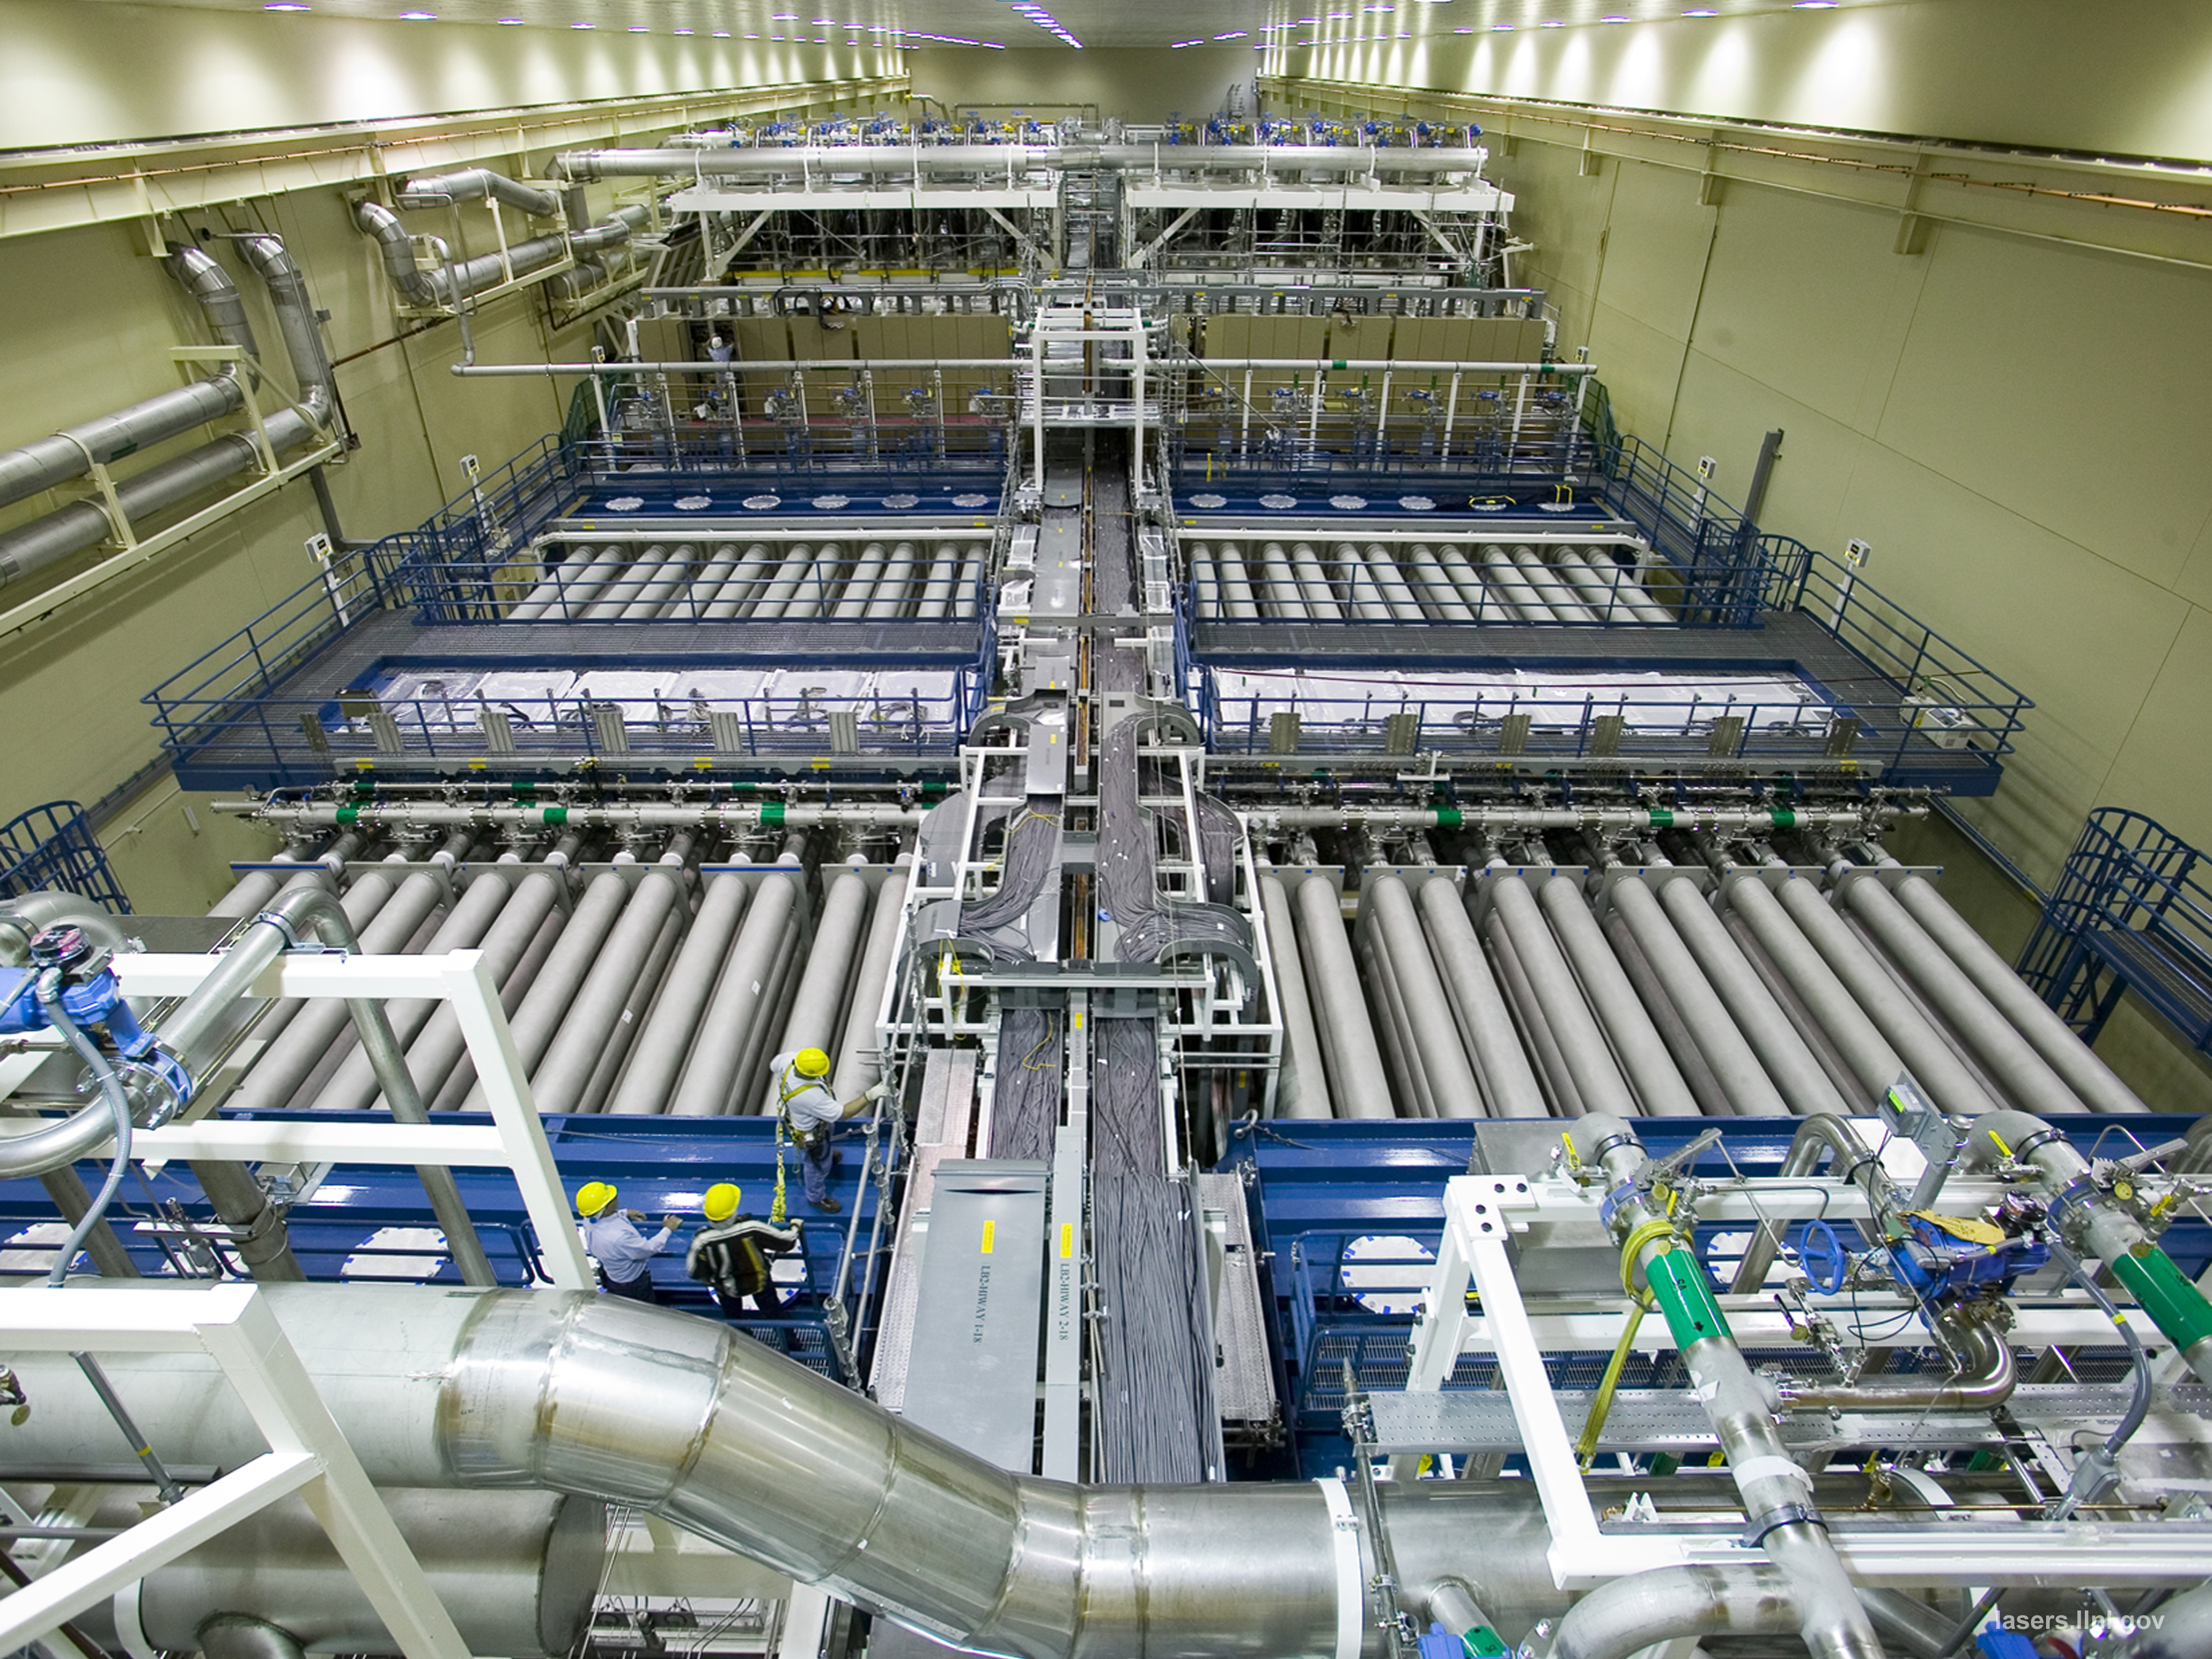
\includegraphics[width=100truemm]{slike/07_NIF_Laser_Bay.jpg}
\caption{Eden najmočnejših laserskih sistemov na svetu, ki doseže 
$500~\si{\tera\watt}$ moči v sunku. \\Vir: National Ignition Facility, Livermore, Kalifornija.}
\label{fig:NIF}
\end{figure}

Moči svetlobe, ki jih oddajajo najmočnejši laserski sistemi, imajo zelo velike
vrednosti. Najmočnejši zvezno delujoči laserji dosegajo tako moči prek 
$\sim 100~\si{\kilo\watt}$. Še bistveno večje moči pa dosegajo sunkovni laserji, 
saj lahko dosežejo moč tudi $\sim 10^{15}~\si{\watt}$. 
Vendar so sunki tako velike svetlobne moči izredno kratki, tipično reda pikosekunde, tako da
znaša celotna moč v takem sunku svetlobe tako 'le' $\sim \si{\kilo\joule}$. Dodaten 
parameter pri tako močnih sunkovnih laserjih je čas, ki poteče med dvema zaporednima
sunkoma. Najmočnejši laserski sistemi tako lahko izsevajo največ nekaj sunkov dnevno. 

\section{He-Ne laser}
\index{Laser!He-Ne}

Kot prvi primer si oglejmo helij-neon (He-Ne) laser, ki je bil prvi zvezno 
delujoči laser in je še danes zelo razširjen. Najpogosteje deluje 
pri valovni dolžini $632,8~\si{\nano\metre}$ v rdečem delu spektra, poleg 
tega pa tudi pri infrardečih $1,15~\si{\micro\metre}$ in 
$3,39~\si{\micro\metre}$ ter nekaterih drugih
valovnih dolžinah v oranžnem in zelenem delu spektra. Laser deluje v zveznem 
načinu delovanja s tipičnimi močmi $0,5 - 100~\si{\milli\watt}$.

Slika~(\ref{fig:HeNeE}) kaže relevantne energijske nivoje helija in neona. 
\index{Energijski nivoji!He-Ne}
\index{Trinivojski sistem}
Atome helija
s trki z elektroni vzbudimo v eno izmed dveh dolgoživih metastabilnih stanj $2^3S$ ali
$2^1S$ z razpadnima časoma $0,1~\si{\milli\second}$ in $5~\si{\micro\second}$.
Ti dve stanji slučajno praktično sovpadata z dvema stanjema neona ($4s$ in $5s$). 
Ko v helij dodamo razmeroma majhno količino neona, se energija s trki 
prenese z vzbujenih helijevih atomov na atome neona, ki s tem preidejo v 
že omenjeni vzbujeni stanji, helijevi atomi pa se vrnejo v osnovno stanje. 
Majhna energijska razlika med nivoji helija in neona (okoli $1,2~\si{\tera\hertz}$) pri 
tem preide v kinetično energijo obeh atomov. 
\begin{figure}[h]
\centering
\def\svgwidth{100truemm} 
\input{slike/07_HeNeE.pdf_tex}
\caption{Shema energijskih nivojev v He-Ne laserju. Nivoji helija so označeni
z modro in nivoji neona z zeleno, laserski prehodi pa z rdečimi barvami in pripisano
ustrezno valovno dolžino.}
\label{fig:HeNeE}
\end{figure}

Znano rdečo svetlobo He-Ne laserja z valovno dolžino $632,8~\si{\nano\metre}$ dobimo 
pri prehodu iz stanja $5s$ v eno od stanj $3p$. Pri tem je življenjski čas 
stanja $5s$ okoli $100~\si{\nano\second}$, stanja $3p$ pa okoli $10~\si{\nano\second}$.
Spodnji $3p$ nivo se prazni s spontano emisijo v metastabilno stanje $3s$. 
V njem se atomi nabirajo, saj so dipolni sevalni prehodi v osnovno stanje prepovedani,
in atomi le s trki ob steno cevi prehajajo v osnovno stanje. Da pospešimo
praznjenje spodnjega nivoja in povečamo obrnjeno zasedenost, moramo torej 
zmanjšati premer razelektritvene cevi. Zaradi gibanja atomov je spektralna 
črta Dopplerjevo razširjena\index{Dopplerjeva razširitev}. 

Lasersko delovanje dobimo tudi pri prehodu iz $5s$ v stanje $4p$, pri katerem 
ima izsevana svetloba valovno dolžino $3,39~\si{\micro\metre}$. 
Ojačenje je za ta prehod celo precej večje kot za
prehod pri $632,8~\si{\nano\metre}$, deloma zaradi nižje frekvence 
(glej zvezo med Einsteinovima koeficientoma $A$ in $B$, enačba~\ref{4.27}), 
deloma pa zaradi kratke življenjske dobe spodnjega laserskega nivoja $4p$. 
Zato bi pričakovali, da bo He-Ne laser svetil v infrardečem območju in ne vidnem. 
To delno prepreči absorpcija v steklu, delno pa izgube namerno povečamo s selektivno odbojnostjo
resonatorskih zrcal, ki dvigne prag delovanja za $3,39~\si{\micro\metre}$ 
nad prag za $632,8~\si{\nano\metre}$. V nekaterih primerih v laser dodamo
celico metana, ki infrardečo svetlobo močno absorbira, rdeče pa ne.
Omenimo še prehode iz stanja $4s$, ki ga dosežejo neonovi atomi s trki
z vzbujenimi helijevimi atomi iz nivoja $2^3S$. Prehod $4s$ v $3p$, ki da svetlobo
pri $1,15~\si{\micro\metre}$, je bil prvi opaženi prehod v He-Ne laserjih.

Tipičen He-Ne laser je razmeroma preprosto zgrajen (sliki~\ref{fig:HeNeShema}
in \ref{fig:Iskra}).\index{Laser!zgradba}
V razelektritveni cevi (napetost  $\sim 1~\si{\kilo\volt}$), skozi
katero teče električni tok ($\sim 10~\si{\milli\ampere}$), 
se nahaja mešanica helija in neona v razmerju 
$5:1 - 10:1$. Skupni tlak v cevi je nizek, le okoli $3~\si{\milli\bar}$, 
cev pa je tipično dolga okoli $0,5~\si{\metre}$ s premerom $1-2~\si{\milli\metre}$.  
Cev na obeh straneh zapirata okni, ki sta nagnjeni za Brewstrov kot (glej enačbo~\ref{eq:Brew}), 
tako da so izgube pri odboju za eno polarizacijo kar se da majhne.
Izhodna svetloba iz laserja je zato seveda polarizirana. V manjših laserjih
so namesto Brewstrovih oken na razelektritveno cev privarjena kar
resonatorska zrcala. Tak laser je nepolariziran. 
Razelektritvena cev je obdana z dvema ukrivljenima zrcaloma, 
ki imata zelo veliko odbojnost za izbrano valovno dolžino.
Nekaj tipičnih podatkov za He-Ne laser je zbranih v tabeli~(\ref{tab:Ar}).
\begin{figure}[h]
\centering
\def\svgwidth{100truemm} 
\input{slike/07_HeNeShema.pdf_tex}
\caption{Shema He-Ne laserja: R - razelektritvena cev, IZ - izhodno zrcalo, Z - zrcalo
z veliko odbojnostjo, B - Brewstrovi okni}
\label{fig:HeNeShema}
\end{figure}

\begin{figure}[h]
\centering
\includegraphics[width=120truemm]{slike/07_HeNe.jpg}
\caption{Primer starejšega He-Ne laserja, izdelanega v Sloveniji}
\label{fig:Iskra}
\end{figure}

He-Ne laserji so preprosti, stabilni, zanesljivi, poceni, imajo visoko kvaliteto žarka
in dolgo služijo (do 50 000 ur).
Danes jih sicer izrivajo polprevodniški laserji, vendar so še vedno v uporabi
v merilnih napravah, v optičnih čitalnih sistemih, v šolah, v raziskovalnih 
laboratorijih za interferometrijo, holografijo itd. Na njem je osnovan tudi 
sekundarni standard za meter.

\section{Argonski ionski laser}
\index{Laser!argonski}
\index{Štirinivojski sistem}
Kot drugi primer plinskega laserja obravnavajmo argonski ionski (Ar$^+$) laser,
ki je najbolj poznan po zveznem delovanju v modrem in zelenem delu spektra pri 
valovnih dolžinah $488~\si{\nano\metre}$ in $514,4~\si{\nano\metre}$, deluje 
pa tudi v bližnjem ultravijoličnem območju. Tipične moči delovanja argonskega laserja
so $100~\si{\milli\watt} - 50~\si{\watt}$.

Kot večino drugih plinskih laserjev tudi tega črpamo z električnim tokom.
Atome argona vzbudimo s trki z elektroni v ione argona, ti pa z nadaljnjimi
trki preidejo v vzbujena stanja. Obrnjeno zasedenost
dosežemo med nivojema $4p$ in $4s$ (slika~\ref{fig:ArE}). 
Ta dva nivoja vsebujeta veliko podnivojev, zato je tudi prehodov med
njima zelo veliko. Argonski laser tako seva pri več kot tridesetih različnih
valovnih dolžinah, najznačilnejši sta že omenjeni 488~nm in 514,5~nm. 
Življenjski čas zgornjega nivoja $\sim 10^{-8}~\si{\second}$ je približno 
desetkrat daljši od življenjskega časa spodnjega nivoja, od koder se ioni
z rekombinacijo z elektroni vrnejo v osnovno stanje atoma. Tudi pri tem laserju
je poglavitni vzrok za razširitev črte \index{Dopplerjeva razširitev}Dopplerjev 
pojav.\index{Energijski nivoji!Argon}

\begin{figure}[h]
\centering
\def\svgwidth{80truemm} 
\input{slike/07_ArE.pdf_tex}
\caption{Shema energijskih nivojev v Ar$^+$ laserju}
\label{fig:ArE}
\end{figure}

Argonski laser je v osnovi zgrajen podobno kot He-Ne laser. \index{Laser!zgradba}
V razelektritveni cevi
(tipična dolžina $1~\si{\metre}$ in premer $1-2~\si{\milli\metre}$)
se nahaja argon pri pritisku okoli $10~\si{\milli\bar}$. Ker gre pri 
vzbujanju atomov argona za dvostopenjski proces, mora biti električni tok, 
s katerim dosežemo obrnjeno zasedenost, precej velik, lahko tudi nekaj deset amperov. 
Pri tipični napetosti nekaj kV to pomeni, da so potrebne velike električne moči, 
pogosto več deset $\si{\kilo\watt}$, in močnejši argonski laserji so zato zaradi 
velike količine odvečne toplote najpogosteje vodno hlajeni.

\begin{figure}[h]
\centering
\def\svgwidth{110truemm} 
\input{slike/07_ArShema.pdf_tex}
\caption{Poenostavljena shema Ar laserja s prizmo: R - razelektritvena cev, 
IZ - izhodno zrcalo, Z - zrcalo z veliko odbojnostjo, B - Brewstrovi okni, 
P - prizma
}
\label{fig:ArS}
\end{figure}

V argonskih laserjih pogosto ustvarimo tudi vzdolžno magnetno polje, ki preprečuje 
elektronom, da bi predčasno zapustili ojačevalno območje in trčili v steno. S
tem se poveča izhodna moč laserja, hkrati pa preprečuje poškodbe na stenah, ki bi jih 
lahko povzročili visokoenergijski elektroni. Iz istega razloga so pri močnejših
laserjih zrcala izven plinske cevi. 

V resonator argonskega laserja pa moramo vgraditi še en dodaten element, ki omogoči
izbiro ene same spektralne črte. Najpogosteje za ta frekvenčno selektiven element
uporabimo kar majhno prizmo pred enim od obeh zrcal (slika~\ref{fig:ArS}). Zaradi disperzije
v prizmi se snopi različnih valovnih dolžin lomijo pod različnimi koti in le tisti 
snop, ki vpada pravokotno na zrcalo, je ojačan. Z vrtenjem prizme ali zrcala lahko 
tako izberemo valovno dolžino ojačene svetlobe. Nekaj tipičnih podatkov za argonski
laser je zbranih v tabeli~(\ref{tab:Ar}).

Argonski laser je zanesljiv in daje zelo kvaliteten osnovni Gaussov snop pri eni
sami frekvenci. Zato se dosti uporablja v optični spektroskopiji,
interferometriji, holografiji in merilni tehniki. Deluje lahko v zveznem načinu,
zaradi razmeroma široke črte ojačenja pa ga uporabljamo tudi za fazno uklenjen
sunkovni laser z dolžino sunkov okoli $150~\si{\pico\second}$. 
V kombinaciji s kriptonovim laserjem, ki je zelo podoben argonskemu, le da deluje
v rdečem in oranžnem delu spektra, se uporablja tudi v zabavni industriji.
V zadnjem času ga vse bolj izrivajo polprevodniški laserji ali pa frekvenčno
podvojeni Nd:YAG. 

\section{Laser na ogljikov dioksid}
\index{Laser!CO$_2$}
Do zdaj opisani laserji so delovali na elektronskih prehodih v atomih oziroma ionih. 
Laser na ogljikov dioksid pa deluje na prehode med vibracijskimi stanji molekul 
CO$_2$, pri čemer elektroni ostanejo v osnovnem stanju.
Zaradi majhnih energijskih razlik med vibracijskimi stanji deluje
tak laser v infrardečem delu spektra, najpogosteje pri 
$9,6~\si{\micro\metre}$ in $10,6~\si{\micro\metre}$. Laser deluje v zveznem
in v sunkovnem načinu, odlikuje ga pa zelo velik izkoristek ($~\sim 30~\%$) in 
posledično zelo velike moči, $1~\si{\watt} - 10~\si{\kilo\watt}$. 

Preden opišemo delovanje laserja, si na kratko oglejmo še nihajna stanja molekule 
ogljikovega dioksida. Molekula CO$_2$ je v osnovnem stanju linearna molekula 
(slika~\ref{fig:CO2}\,a). 
Za molekule take oblike obstajajo trije osnovni načini nihanja atomov glede na težišče:
atoma kisika nihata simetrično vzdolž osi molekule, pri čemer ogljik miruje --
simetrični razteg (slika~\ref{fig:CO2}\,b), atomi nihajo v smeri pravokotno na 
os -- upogib (slika~\ref{fig:CO2}\,c) in atoma kisika se gibljeta v isti smeri 
vzdolž osi, ogljik pa v nasprotni smeri -- asimetrični razteg (slika~\ref{fig:CO2}\,d). 
Pri tem ima najvišjo frekvenco asimetrični razteg, najnižjo pa upogib. 
Vsako vibracijsko stanje lahko razstavimo na osnovne nihajne načine in 
ga opišemo s številom energijskih kvantov v posameznem osnovnem nihanju, 
torej s trojico celih števil $(n_1,n_2,n_3)$. Stanje 100 tako opisuje
osnovni simetrični razteg, stanje 010 osnovno upogibno nihanje, stanje 001 pa 
osnovni asimetrični razteg.

\begin{figure}[h]
\centering
\def\svgwidth{100truemm} 
\input{slike/07_CO2.pdf_tex}
\caption{Molekula CO$_2$ (a) in trije osnovni načini nihanja molekule:
simetrični razteg (b), upogib (c) in asimetrični razteg (d)}
\label{fig:CO2}
\end{figure}

Vibracijska stanja molekule vzbudimo z električnim tokom skozi plin. 
\index{Energijski nivoji!CO$_2$}
\index{Štirinivojski sistem}
Pri tem v razelektritveno cev dodamo dušik (N$_2$) in podobno kot pri He-Ne laserju
se tudi CO$_2$ črpa predvsem preko trkov z dušikovimi molekulami. 
Dušikova molekula je dvoatomna in ima zato zgolj eno vibracijsko stanje, ki po energiji
praktično sovpada z energijo stanja 001 (slika~\ref{fig:CO2E}). Iz tega gornjega
stanja prehajajo molekule v stanje 100 ($10,6~\si{\micro\metre}$) ali v stanje
020 ($9,6~\si{\micro\metre}$). Da pospešimo prehod nazaj v osnovno stanje, 
plinski mešanici dodamo še helij, s katerim trkajo molekule.
Razmerje parcialnih tlakov je tako navadno 1:1:8 za CO$_2$:N$_2$:He pri tlaku $1~\si{\milli\bar}$. 
Pri tako nizkih tlakih je poglavitna razširitev spektralne črte Dopplerjeva, 
\index{Dopplerjeva razširitev}ki 
pa je v primerjavi z ostalimi plinskimi laserji zaradi nizih frekvenc zelo majhna,
le okoli $70~\si{\mega\hertz}$. V laserskih sistemih, kjer je tlak plinov večji,
prevlada razširitev zaradi medmolekulskih trkov. Pri tlakih okoli $20~\si{\bar}$
znaša razširitev že okoli $500~\si{\giga\hertz}$, kar omogoča izdelavo fazno uklenjenih 
sunkovnih laserjev s sunki dolžine $\sim 1~\si{\pico\second}$. Nekaj tipičnih podatkov 
za laser na ogljikov dioksid je zbranih v tabeli~(\ref{tab:Ar}).

\begin{figure}[h]
\centering
\def\svgwidth{95truemm} 
\input{slike/07_CO2E.pdf_tex}
\caption{Shema vibracijskih nivojev v CO$_2$ laserju}
\label{fig:CO2E}
\end{figure}

Najpreprostejši laser na ogljikov dioksid \index{Laser!zgradba} 
je po svoji zgradbi podoben že obravnavanim plinskim laserjem. 
Razelektritvena cev (polmer $\sim 1~\si{\centi\metre}$ in dolžina $0,5-2~\si{\metre}$) 
je na obeh koncih zaključena z Brewstrovima oknoma in zrcaloma, pri čemer moramo paziti,
da elementi prepuščajo oziroma odbijajo infrardečo svetlobo. Ker lahko deluje
laser pri zelo veliko različnih valovnih dolžinah, dodamo frekvenčno selektiven
člen, na primer uklonsko mrežico (slika~\ref{fig:CO2S}).\index{Uklonska mrežica}

\begin{figure}[h]
\centering
\def\svgwidth{100truemm} 
\input{slike/07_CO2Shema.pdf_tex}
\caption{Poenostavljena shema najpreprostejšega CO$_2$ laserja: R - razelektritvena cev, 
IZ - izhodno zrcalo, Z - zrcalo z veliko odbojnostjo, B - Brewstrovi okni, 
U - uklonska mrežica
}
\label{fig:CO2S}
\end{figure}

Poleg običajnih zaprtih sistemov poznamo tudi laserje z vzdolžnim ali prečnim pretokom, 
valovodne laserje ... Razlikujejo se po svojih specifikacijah in vrsti uporabe.
Laserji na ogljikov dioksid se največ uporabljajo v industriji za zahtevne 
obdelave materialov, na primer za rezanje 
kovin, vrtanje, ablacijo, varjenje, pa tudi za vojaške in medicinske namene.
Obdelava z laserji omogoča veliko natančnost, čistočo in je zelo fleksibilna.

\begin{table}
\small
\begin{center}
\begin{tabular}{|l|c|c|c|c|}\hline
Laser & He-Ne & Ar$^+$ & CO$_2$ & ekscimer\\ \hline
Valovna dolžina  $\lambda$ & $632,8~\si{\nano\metre}$& $488$ in
$514,5~\si{\nano\metre}$ & $9,6$ in $10,6~\si{\micro\metre}$ & UV
\\ \hline
Verjetnost za spontani prehod $A$ & $3,4 \times 10^6/\si{\second}$ & 
$7,8 \times 10^7/\si{\second}$ & $0,25/\si{\second}$ & $\sim 10^8/\si{\second}$ \\ \hline
Presek za stimulirano emisijo $\sigma$ & $3 \times 10^{-17}~\si{\metre}^2$&  $2,6 \times 10^{-16}~\si{\metre}^2$ & $3 \times 10^{-22}~\si{\metre}^2$ & $ 10^{-20}~\si{\metre}^2$ \\ \hline
Spektralna širina črte $\Delta \nu$ & $1,5 \times 10^{9}~\si{\hertz}$ & 
$3,5 \times 10^{9}~\si{\hertz}$ &$7 \times 10^{7}~\si{\hertz}$ & $10^{13}~\si{\hertz}$ \\ \hline
Obrnjena zasedenost $\Delta N/V$ & $5 \times 10^{15}/\si{\metre}^3$ & $2 \times 10^{15}/\si{\metre}^3$ & $3 \times 10^{21}/\si{\metre}^3$ & $10^{20}/\si{\metre}^3$\\ \hline
\end{tabular}
\caption{Izbrani podatki za He-Ne, Ar$^+$, CO$_2$ in tipičen ekscimerni laser}
\index{Laser!He-Ne}
\index{Laser!argonski}
\index{Laser!CO$_2$}
\index{Laser!ekscimerni}
\label{tab:Ar}
\end{center}
\end{table}

\section{Ekscimerni laser}
\index{Laser!ekscimerni}
Ekscimerji ({\it excited dimer, excimer}) so vzbujena vezana stanja dveh atomov, 
ki bi se v osnovnem stanju ne vezala. Za laserje so zanimivi predvsem ekscimerji
težkih žlahtnih plinov in halogenov, na primer Ar$_2^*$ ($126~\si{\nano\metre}$), 
Kr$_2^*$ ($146~\si{\nano\metre}$), Xe$_2^*$ ($172~\si{\nano\metre}$),
ArF ($193~\si{\nano\metre}$), KrF ($248~\si{\nano\metre}$), 
XeCl ($308~\si{\nano\metre}$), ArBr ($161~\si{\nano\metre}$), 
NeF ($108~\si{\nano\metre}$) ... Te molekule obstajajo samo v vzbujenem stanju,
v osnovnem stanju pa je odbojna sila med atomoma prevelika in molekula neobstojna.
Vsi našteti primeri oddajajo lasersko svetlobo v
ultravijoličnem področju, ki ga drugi laserski sistemi le težko pokrivajo. 
Ekscimerni laserji delujejo v sunkih, pri čemer je tipična oddana energija v sunku 
$\sim 1~\si{\joule}$, dolžina sunka $10-100~\si{\nano\second}$ in repeticija 
$\sim 100~\si{\hertz}$.

Vezano stanje dveh atomov dobimo, kadar je ionizacijska energija prvega
atoma manjša od vsote elektronske afinitete drugega atoma in
elektrostatične energije vezave obeh ionov. Vzemimo za primer klor in
kripton. Ionizacijska energija kriptona v osnovnem stanju je 14~eV, v
vzbujenem pa 5~eV. Elektronska afiniteta klora je 3,75~eV in
elektrostatična vezavna energija KrCl okoli 7~eV. Tako je za nastanek
molekule KrCl v osnovnem stanju potrebno dodati okoli 4~eV, pri tvorbi
molekule v vzbujenem stanju pa se sprosti okoli 6~eV. Približno obliko
celotne potencialne energije molekule KrCl v osnovnem in vzbujenem stanju
kaže slika~(\ref{fig:exE}). Molekula, ki je vezana v vzbujenem stanju, po
sevalnem prehodu v osnovno stanje takoj razpade, zato je zelo lahko doseči
obrnjeno zasedenost. Pri tem je razpadni čas vezanega stanja $\sim~10~\si{\nano\second}$,
spodnjega nevezanega pa okoli $0,1~\si{\pico\second}$.
Spektralna širina prehoda je precej velika, okoli $1~\si{\nano\metre}$.
Da nastanejo ekscimeri, vzbujamo mešanico 
plinov (žlahtnega plina ali mešanice žlahtnega in halogenega plina) v heliju. Ker je pritisk
razmeroma velik (npr. 2 ali $3~\si{\bar}$), je vzbujanje prečno, podobno kot pri 
nekaterih izvedbah CO$_2$ laserja. Nekaj tipičnih podatkov 
za ekscimerni laser je zbranih v tabeli~(\ref{tab:Ar}).
\index{Energijski nivoji!ekscimer}

Ekscimerni laserji delujejo v sunkih s precej veliko energijo in se uporabljajo 
v industriji materialov, mikroprocesorjev, fotolitografiji in medicini, predvsem 
oftalmologiji in kirurgiji.
\begin{figure}[h]
\centering
\def\svgwidth{50truemm} 
\input{slike/07_exE.pdf_tex}
\caption{Shema energije v odvisnosti od razdalje med jedroma atomov. V vzbujenem stanju
se atoma povežeta v molekulo, po prehodu v nižji nivo pa atoma disociirata.}
\label{fig:exE}
\end{figure}


\section{Neodimov laser}
Druga skupina laserjev so trdninski laserji. Taki laserji
so osnovani na elektronskih prehodih v ionih primesi, ki jih dodamo v kristal ali steklo,
črpamo pa jih optično. Primesi so praviloma redke zemlje ali prehodne kovine, 
kristali pa so navadno oksidi ali fluoridi. Izdelava ojačevalnih sredstev na osnovi stekla
je bistveno bolj preprosta in poceni, vendar ima steklo precej nižjo toplotno prevodnost
od kristalov in se zato bolj greje. 
Začeli bomo z opisom dveh primerov neodimovega laserja, Nd:YAG in Nd:steklo. Podobne laserje dobimo, 
če v YAG kristalu namesto z neodimom itrijeve ione nadomestimo z iterbijem ($1030~\si{\nano\metre}$) ali erbijem ($2940~\si{\nano\metre}$).

\subsection{Nd:YAG}
\index{Laser!Nd:YAG}
Najpomembnejši predstavnik je Nd:YAG laser, v katerem je ojačevalno sredstvo
itrij-aluminijev granat (Y$_3$Al$_5$O$_{12}$, YAG) s primesmi neodimovih ionov Nd$^{3+}$. 
Neodimov laser deluje pri valovni dolžini $1,064~\si{\micro\meter}$ ali frekvenčno podvojeni
$532~\si{\nano\metre}$. Laser lahko deluje v zveznem 
načinu pri močeh $5-100~\si{\watt}$ ali sunkovnem z dolžino sunkov okoli 
$100~\si{\nano\second}$ in energijo sunka $\sim 1~\si{\joule}$.

Neodimov laser je primer štirinivojskega laserskega sistema, 
\index{Štirinivojski sistem}pri čemer je 
laserski prehod med stanjema $^4$F$_{3/2}$ in $^4$I$_{11/2}$ iona neodima 
(slika~\ref{fig:NdE}). S svetlobo višje frekvence 
(tipično okoli $800~\si{\nano\metre}$) črpamo elektrone v višje nivoje, ki hitro 
preidejo v zgornji laserski nivo. Življenjski čas višjega nivoja je 
okoli $230~\si{\micro\second}$, spodnjega pa precej krajši, zato je 
lahko doseči veliko obrnjeno zasedenost. Spodnje stanje je dovolj visoko nad 
osnovnim, da pri sobni temperaturi v ravnovesju ni znatno zasedeno. Zato je 
prag neodimovega laserja nizek in je lahko doseči zvezno stacionarno delovanje, 
prav tako dobro pa deluje tudi v sunkih. Razširitev črte je homogena in je predvsem posledica
termičnega nihanja kristalne mreže. Laser je odličen za delovanje s preklopom dobrote, 
zaradi ozke črte pa z uklepanjem faz oddaja zelo kratke sunke (nekaj ps). 
\index{Energijski nivoji!Nd:YAG}
\begin{figure}[h]
\centering
\def\svgwidth{85truemm} 
\input{slike/07_NdE.pdf_tex}
\caption{Shema energijskih nivojev v Nd$^{3+}$ laserju}
\label{fig:NdE}
\end{figure}

Za črpanje uporabljamo diodne laserje ali močne ksenonove svetilke za zvezno delovanje 
ter podobne bliskovne luči za sunkovno delovanje (slika~\ref{fig:Nd}\,a). 
Aktivna snov v laserju je v obliki paličice dolžine od nekaj cm do dobrih 
$10~\si{\centi\metre}$ in širine do okoli $1~\si{\centi\metre}$. 
V kristalu YAG neodimovi ioni nadomestijo približno $1~\%$ itrijevih, zato ojačevalno
sredstvo na videz ni prozorno, temveč rahlo rožnato (slika~\ref{fig:Nd}\,b). 
Aktivna paličica in svetilka sta vgrajeni v cilindrično ali eliptično votlino z 
zrcalnimi ali belimi stenami, tako da se čim večji del črpalne svetlobe absorbira v 
laserski paličici (slika~\ref{fig:Nd}\,c).

\begin{figure}[h]
\centering
\def\svgwidth{120truemm} 
\input{slike/07_Nd.pdf_tex}
\caption{Ksenonska bliskovna svetilka (a), ojačevalno sredstvo v Nd:YAG laserju (b) 
in shema eliptične črpalne votline (c)}
\label{fig:Nd}
\end{figure}

Pri črpanju s ksenonsko svetilko je le manjši del izsevane svetlobe v
absorpcijskih pasovih, zato je izkoristek črpanja razmeroma slab, tipično 
pod $0,01~\%$. Za izhodno moč zvezno delujočega Nd:YAG laserja nekaj deset wattov je tako
potrebna električna moč nekaj kW. Velika večina porabljene moči 
gre v gretje, zato je v laserjih z nekoliko večjo povprečno
močjo potrebno vodno hlajenje. Gretje povzroča tudi toplotne deformacije
laserske paličice, kar lahko močno spremeni lastnosti resonatorja. Toplotni
učinki so ena poglavitnih praktičnih težav pri izdelavi neodimovih
laserjev s klasičnimi svetilkami . Danes prevladuje
 črpanje z diodnimi laserji, ki svetijo v območju največje
absorpcije Nd$^{3+}$. Črpanje je lahko prečno ali pa vzdolžno (slika~\ref{fig:NdS}). 
Pri diodnem črpanju je izkoristek dosti večji in je manj gretja, kar omogoča 
bolj kompaktno konstrukcijo in boljšo stabilnost izhodne moči.
\index{Laser!zgradba} 
\begin{figure}[h]
\centering
\def\svgwidth{120truemm} 
\input{slike/07_NdS.pdf_tex}
\caption{Shema vzdolžnega diodnega črpanja Nd:YAG laserja. O - ojačevalno sredstvo, 
IZ - izhodno zrcalo, D - dikroično zrcalo, 
prepustno za črpalno svetlobo in odbojno za lasersko, DL - diodni 
laser za črpanje, L - leča
}
\label{fig:NdS}
\end{figure}

Neodimovi laserji so zelo razširjeni, tako v osnovni kot tudi v frekvenčno 
podvojeni različici. 
Najbolj uporabni so za obdelavo materialov (na primer vrtanje in varjenje, 
litografija) ter v medicini (dermatologija in endoskopska kirurgija). 
Pomemben proizvajalec Nd:YAG laserjev 
za medicinske namene je tudi podjetje Fotona iz Ljubljane. 

\begin{table}[h]
\small
\begin{center}
\begin{tabular}{|l|c|c|c|}\hline
Laser & Nd:YAG & Nd:steklo & Ti:safir \\ \hline
Valovna dolžina  & $1064~\si{\nano\metre}$ & $1050~\si{\nano\metre}$ & 
 $660-1180~\si{\nano\metre}$\\ \hline
Verjetnost za spontani prehod $A$ & $4 \times 10^3/\si{\second}$ & $3 \times 10^3/\si{\second}$
& $3 \times 10^5/\si{\second}$\\ \hline
Presek za stimulirano emisijo $\sigma$ & $3 \times 10^{-23}~\si{\metre}^2$ &
$3 \times 10^{-24}~\si{\metre}^2$ & $3 \times 10^{-23}~\si{\metre}^2$\\ \hline
Spektralna širina črte $\Delta \nu$ & $1,3 \times 10^{11}~\si{\hertz}$ &
$7 \times 10^{12}~\si{\hertz}$ & $1 \times 10^{14}~\si{\hertz}$\\ \hline
Gostota obrnjene zasedenosti $\Delta N/V$ & $1,6 \times 10^{23}/\si{\metre}^3$ &
$8 \times 10^{23}/\si{\metre}^3$ & $6 \times 10^{23}/\si{\metre}^3$\\ \hline
\end{tabular}
\caption{Tipični podatki za Nd:YAG, Nd:steklo in Ti:safirni laser}
\index{Laser!Nd:YAG}
\index{Laser!Nd:steklo}
\index{Laser!Ti:safir}
\label{tab:nd}
\end{center}
\end{table}

\subsection{Nd:steklo}
\index{Laser!Nd:steklo}
Namesto v ustrezen kristal lahko neodimove ione Nd$^{3+}$ vgradimo tudi v steklo. 
Tak laser deluje pri valovni dolžini $1,050~\si{\micro\meter}$ v sunkovnem načinu 
s preklopom dobrote ali z uklepanjem faz z energijami sunkov $~\sim 1~\si{\joule}$.
Z ojačevalniki dosežemo energije sunka nad $100~\si{\kilo\joule}$. 
Zaradi amorfne strukture stekla in posledično 
nehomogenega lokalnega polja je laserska črta nehomogeno razširjena.
\index{Spektralna črta!nehomogena razširitev}
Ojačenje je manjše kot v Nd:YAG in za prag laserskega delovanja je
potrebna precej večja moč črpanja. Laserji Nd:steklo zato delujejo le v sunkovnem
načinu, kjer pa so za velike energije celo boljši od Nd:YAG. Zaradi
manjšega ojačenja pri dani obrnjeni zasedenosti je v laserju s preklopom
dobrote mogoče doseči večjo načrpanost, ne da bi prišlo do praznjenja
zaradi ojačevanja spontanega sevanja v enem preletu paličice. Problem teh laserjev
predstavlja nizka toplotna prevodnost stekla, ki omejuje repeticijo sunkov.
Velika širina črte je zelo primerna za delovanje v načinu uklepanja faz, s 
katerim dosegamo ultrakratke sunke ($\sim 100~\si{\femto\second}$). 

\begin{remark}
Energije izsevanih sunkov je mogoče še povečati z ojačevalniki. Med največjimi je
laserski sistem Nd:steklo v Rochestru (New York), ki ga uporabljajo
za raziskave fuzije. Okoli $1~\si{\nano\second}$ dolg sunek iz osnovnega laserja razdelijo na
deset ojačevalnih vej, ki so dolge po $180~\si{\metre}$.
Končna energija sunka je nad $\sim 1~\si{\mega\joule}$. Z njim z vseh strani posvetijo na
kroglico iz devterija in tritija, ki se dovolj segreje in stisne, da pride
do njunega zlivanja. Vršna moč laserskega sunka je okoli $10^{15}$~W. 
Če laserski snop zberemo na površino 1~mm$^2$, dobimo električno poljsko jakost
okoli $5 \times 10^{11}$~V/m, kar je približno enako polju v vodikovem atomu.
\end{remark}

\section{Titan-safirni laser}
\index{Laser!Ti:safir}
Titan-safirni laser (Ti:safir) je trdninski laser, pri katerem so v kristal safirja
Al$_2$O$_3$ primešani ioni titana Ti$^{3+}$. Njegova najpomembnejša značilnost je
zvezna nastavljivost valovne dolžine v zelo širokem frekvenčnem pasu 
($600-1180~\si{\nano\metre}$) z največjo učinkovitostjo pri okoli $800~\si{\nano\metre}$. Deluje
v zveznem načinu z močmi do $50~\si{\watt}$ in v fazno uklenjenem načinu sunkovno 
z dolžino sunkov do $10~\si{\femto\second}$ z vršnimi močmi nad $10^{12}~\si{\watt}$. 
\index{Energijski nivoji!Ti:safir}
\begin{figure}[h]
\centering
\def\svgwidth{90truemm} 
\input{slike/07_TiE.pdf_tex}
\caption{Energijski nivoji v titan-safirnem laserju. Dva nivoja sta zaradi vibracij
razcepljena na veliko število podnivojev, ki pa se med seboj deloma prekrivajo.
Zelo podobna je tudi shema energijskih nivojev organskih barvil. 
}
\label{fig:TiE}
\end{figure} 

Ojačevalno sredstvo v titan-safirnem laserju je aluminijev oksid, v katerem 
približno $0,2~\%$ aluminijevih ionov nadomestimo s titanovimi. Titanovi ioni imajo 
v taki konfiguraciji zgolj eno vzbujeno stanje, vendar se zaradi sklopitve s fononi
vibracijski nivoji posameznega stanja med seboj prekrivajo in prehod je močno razširjen. 
Z optičnim črpanjem vzbudimo titanov ion iz osnovnega stanja v eno izmed vibracijskih 
stanj vzbujenega stanja, ki hitro preide v najnižje vzbujeno stanje. 
Laserski prehod poteka med nižjem vzbujenim stanjem in enim od vibracijskih 
nivojev osnovnega stanja (slika~\ref{fig:TiE}), od koder se vrne v osnovno stanje. Življenjski čas
vzbujenega stanja je kratek ($3,2~\si{\micro\second}$), širina črte pa največja med
vsemi trdninskimi laserji. Ker je vrh absorpcijskega pasu blizu $500~\si{\nano\metre}$,
laser črpamo z zeleno svetlobo (argonski laser za zvezno delovanje oziroma
frekvenčno podvojen neodimov laser za sunkovno). 
Najpomembnejša uporaba je v raziskovalnih laboratorijih za ustvarjanje zelo 
kratkih sunkov svetlobe z dolžino $\sim 10~\si{\femto\second}$. Prevedeno v dolžino 
je to le nekaj valovnih dolžin svetlobe. 

\section{Laserji na organska barvila}
\index{Laser!organska barvila}
Naslednja skupina laserjev so laserji na organska barvila, v katerih
je organsko barvilo raztopljeno v tekočini, praviloma vodi ali alkoholu. 
To so bili prvi laserji z veliko spektralno širino in nastavljivo valovno dolžino
delovanja. Delujejo lahko kot zvezni laserji in z izbiro barvila lahko dosežemo
delovanje v območju $300-1500~\si{\micro\metre}$ pri močeh do $\sim 2~\si{\watt}$, 
široka spektralna širina pa omogoča sunkovno delovanje z uklepanjem faz 
z nekaj femtosekundnimi sunki pri energiji sunka nekaj $100~\si{\joule}$.

Shema energijskih nivojev molekule tipičnega organskega barvila
je zelo podobna shemi energijskih nivojev titan-safirnega laserja (slika~\ref{fig:TiE}).
Vsi elektronski nivoji so razcepljeni v vibracijske in rotacijske podnivoje. 
V toplotnem ravnovesju je molekula na dnu osnovnega elektronskega stanja S$_0$. 
Z absorpcijo vidne svetlobe primerne frekvence preide v neko vzbujeno
singletno stanje $S_1$. Preko trkov z molekulami topila vzbujena barvilna molekula
zelo hitro, v času okoli pikosekunde, preide na dno vzbujenega stanja, od
koder s sevanjem preide nekam v osnovno stanje $S_0$, od tam pa s trki
hitro nazaj na dno osnovnega stanja. Ker
sta obe elektronski stanji zaradi vibracij in rotacij razširjeni, sta 
absorpcijska in emisijska fluorescenčna črta široki. Tipična
širina je blizu 50~nm. Energija izsevane svetlobe je zmanjšana za energijo
prehodov s trki, zato je fluorescenčna črta premaknjena k nižjim
frekvencam od absorpcijske. Absorpcijski in fluorescenčni spekter prehoda $S_0-S_1$
za barvilo rodamin 6G kaže slika~(\ref{fig:RhG}).

\begin{figure}[h]
\centering
\def\svgwidth{80truemm} 
\input{slike/07_RhG.pdf_tex}
\caption{Absorpcijski in emisijski spekter barvila rodamin 6G, ki se uporablja v laserjih}
\label{fig:RhG}
\end{figure} 

\begin{table}[h]
\begin{center}
\begin{tabular}{|l|c|}\hline
Valovna dolžina  & $300 - 1500~\si{\micro\meter}$\\ \hline
Verjetnost za spontani prehod $A$ & $ \sim 10^8/\si{\second}$ \\ \hline
Presek za stimulirano emisijo $\sigma$ & $3 \times 10^{-20}~\si{\metre}^2$ \\ \hline
Spektralna širina črte $\Delta \nu$ & $3 \times 10^{13}~\si{\hertz}$  \\ \hline
Gostota obrnjene zasedenosti $\Delta N/V$ & $ \sim 10^{22}/\si{\metre}^3$ \\ \hline
\end{tabular}
\caption{Tipični podatki za laserje na organska barvila}
\label{tab:orgb}
\end{center}
\end{table}

Laser na organska barvila lahko deluje pri vseh frekvencah znotraj široke
fluorescenčne črte. Zato moramo v resonator vgraditi nek frekvenčno
selektiven element, s katerim lahko nastavljamo frekvenco laserja. Uporabna
je prizma, kot v primeru argonskega laserja, ali pa eno od zrcal nadomestimo 
z uklonsko mrežico, ki je postavljena pod takim kotom, da se po osi resonatorja odbije svetloba
izbrane valovne dolžine.\index{Uklonska mrežica} To lahko spremenimo s spreminjanjem kota nagiba mrežice.
Barvilne laserje črpamo ali z bliskovno lučjo ali z drugim laserjem primerne 
valovne dolžine, na primer argonskim ali ekscimernim laserjem. 
Široko območje ojačevanja barvila nam z uklepanjem faz omogoča dobiti
tudi zelo kratke svetlobne sunke, pod $1~\si{\pico\second}$.

Laserji na organska barvila so uporabni v spektroskopiji, za ločevanje izotopov, v 
medicini (npr. za odstranjevanje ledvičnih kamnov), astronomiji (za umetne laserske zvezde) ...
 
\section{Vlakenski laserji}
\index{Laser!vlakenski laserji}

\section{Polprevodniški laserji}
% 
% Za široko uporabo so danes brez dvoma najpomembnejši polvodniški laserji.
% Njihove glavne značilnosti so majhne dimenzije, neposredno črpanje z
% električnim tokom majhne jakosti in pri nizki napetosti, velik izkoristek,
% preko 20%,
% pri pretvorbi električne moči v svetlobno, in možnost hitre modulacije
% svetlobne moči z modulacijo električnega toka. Poleg tega jih je moč
% integrirati z drugimi polvodniškimi elementi in se za njihovo izdelavo
% uporablja običajna polvodniška tehnologija.
% 
% Polvodniki absorbirajo svetlobo s frekvenco nad energijo prehoda iz
% valenčnega v prevodni pas. Pri tem z vzbuditvijo elektrona iz valenčnega v
% prevodni pas nastane par elektron-vrzel. Ta se lahko rekombinira z
% izsevanjem fotona, kar ustreza spontanemu ali stimuliranemu prehodu v atomih
% in molekulah. Zaradi ohranitve gibalne količine se valovni vektor elektrona
% pri prehodu le zelo malo spremeni, saj je valovni vektor vidne svetlobe
% majhen v primerjavi z vektorjem recipročne mreže polvodniškega kristala.
% To ima pomembno posledico. Najobičajnejša polvodnika, silicij in germanij,
% imata vrh prevodnega pasu v centru Brilluinove cone, to je pri valovnem
% vektorju nič, dno prevodnega pasu pa pri končno velikem valovnem vektorju.
% Zato direkten prehod z dna prevodnega pasu v vrh valenčnega pasu z
% izsevanjem fotona ni možen, potrebna je sočasna emisija ali absorpcija
% fonona, ki poskrbi za ohranitev gibalne količine. Tak proces pa je seveda
% mnogo manj verjeten, zato v siliciju in germaniju v običajni obliki ni
% mogoče dobiti znatnega sevanja s prehodi iz prevodnega v valenčni pas.
% 
% Opisane težave ni pri spojinah iz tretje in pete skupine elementov, na
% primer GaAs, kjer je valenčni pas 1,4 eV nad prevodnim. Na njih so osnovani
% polvodniški laserji.
% 
% Verjetnost za zasedenost elektronskih stanj v termičnem ravnovesju v
% polvodniku je podana s Fermi-Diracovo funkcijo \ref{ts}:
% 
% \begin{equation}  \label{6.1}
% f(E)=\frac{1}{e^{(E-E_F)/k_B T}+1}\;\;.
% \end{equation}
% Pri nizkih temperaturah so zasedena vsa stanja do Fermijeve energije $E_F$,
% nad njo pa so prazna. V čistem polvodniku je $E_F$ na sredini med
% valenčnim in prevodnim pasom, z dodajanjem donorskih primesi pa se
% približuje prevodnemu pasu. Če je koncentracija primesi dovolj velika,
% lahko $E_F$ tudi pri absolutni ničli pride nad dno prevodnega pasu. Tak
% degenriran polvodnik se obnaša podobno kot kovina.
% 
% Če polvodnik ni v termičnem ravnovesju, na primer v p-n spoju, skozi
% katerega teče električni tok, lahko vpeljemo približni Fermijevi energiji 
% $E_{Fv}$ in $E_{Fp}$ posebej za valenčni in prevodni pas. Tak približek je
% dober, kadar je čas, v katerem preidejo vzbujeni elektroni z višjih
% energij na dno prevodnega pasu, dosti krajši od časa prehoda iz prevodnega
% v valenčni pas. Ta pogoj je v polvodnikih, ki jih uporabljamo za laserje,
% navadno zelo dobro izpoljnen. Preko trkov s fononi elektroni preidejo v dno
% prevodenga pasu v pikosekundah, za prehod v valenčni pas, to je za
% rekombinacijo elektrona z vrzeljo, pa so potrebne nanosekunde.
% 
% Neravnovesno stanje, ki ga lahko opišemo z približnima Fermijevima
% energijama, dobimo, kadar v degeneriran polvodnik p-tipa z dovolj veliko
% hitrostjo dodajamo elektrone v prevodni pas. To lahko storimo preko p-n
% spoja, na katerem je napetost v prevodni smeri. Tedaj dobimo položaj, ki ga
% kaže slika \ref{s6.10}. Naj bo $N_p$ gostota elektronov v prevodnem pasu, $I
% $ električni tok skozi spoj, $\tau$ pa čas za rekombinacijo elektrona in
% vrzeli. Velja 
% \begin{equation}  \label{6.2}
% \frac{N_p}{\tau}=\frac{I}{e V}\;,
% \end{equation}
% kjer je V volumen, v katerem se elektroni nahajajo. Po drugi strani je $N_p$
% podana kot integral gostote elektronskih stanj v prevodnem pasu $%
% \rho_p(E)=1/(2\pi^2)(2m_p/\hbar^2)^{3/2}(E-E_g)^{1/2}$, kjer je $m_p$
% efektivna masa prevodnih elektronov, in Fermi- Diracove funkcije: 
% \begin{equation}  \label{6.3}
% N_p=\int_{0}^{\infty}\,\rho_p(E)f_p(E)\,dE
% \end{equation}
% Iz enačb \ref{6.2} in \ref{6.3} lahko izračunamo vrednost $E_{Fp}$ pri
% poljubni temperaturi. Pri $T=0$ je integral preprost in je 
% \begin{equation}  \label{6.4}
% E_{Fp}(T=0)=(2\pi^2)^{2/3}\frac{\hbar^2}{2m_p}\,N_p^{2/3}
% \end{equation}
% $E_{Fp}$ je odvisna od toka skozi spoj in od temperature, kar je pomebno za
% delovanje polvodniškega laserja.
% 
% Naj na p-n spoj vpada svetlobni snop s frekvenco $\omega$, ki je nekoliko
% nad $E_g/\hbar$. Svetloba povzroča prehode med stanji z energijo $E_p$ v
% prevodnem pasu in med stanji z energijo $E_v$ v valenčnem pasu, kot kaže
% slika \ref{s6.11}. Ta stanja se lahko razlikujejo po valovnem vektorju, zato
% moramo verjetnost za stimuliran prehod najprej zapisati za določen valovni
% vektor $\vec{k}$, nato pa sešteti po vseh možnih $\vec{k}$. V primeru
% izotropnih elektronskih pasov je verjetnost za prehod odvisna le od
% velikosti $\vec{k}$. Uporabimo zlato pravilo, kjer upoštevamo, da je
% verjetnost za zasedenost gornjega stanja $f_p(E_p)$ in verjetnost, da je
% spodnje stanje nezasedeno, $1-f_v(E_v)$: 
% \begin{equation}  \label{6.5}
% w_s(k)=\frac{2\pi}{\hbar}|H_{pv}|^2\delta(E_p-E_v- \hbar\omega)
% f_p(E_p)[1-f_v(E_v)]\;,
% \end{equation}
% kjer je $H_{pv}= |p\rangle \hat{x}|v\rangle E $ matrični element za dipolni
% prehod v svetlobnem polju $E$ med prevodnim in valenčnim pasom. Podobno je
% verjetnost za absorpcijo 
% \begin{equation}  \label{6.6}
% w_a(k)=\frac{2\pi}{\hbar}|H_{pv}|^2\delta(E_p-E_v- \hbar\omega)
% f_v(E_v)[1-f_p(E_p)]\;.
% \end{equation}
% 
% Razliko med številom spontanih emisij in absorpcij na enoto volumna dobimo,
% če razliko gornjih verjetnosti seštejemo po vseh $k$: 
% \begin{eqnarray}  \label{6.7}
% N_{pv}-N_{vp}&=&\int[w_s-w_a]\rho(k)\,dk  \nonumber \\
% &=&\frac{2}{\pi\hbar}|H_{pv}|^2 \int[f_p(E_p)-f_v(E_v)]
% \delta(E_p-E_v-\hbar\omega) k^2\,dk\;.
% \end{eqnarray}
% Upoštevli smo, da je gostota stanj $\rho(k)=1/\pi^2 k^2dk$. Štejmo
% energijo od vrha valenčnega pasu. Energija elektronov blizu dna prevodnega
% pasu je $E_g+1/(2m_e)\hbar^2 k^2$, vrzeli pri vrhu prevodnega pasu pa $%
% 1/(2m_h)\hbar^2 k^2$, kjer sta $m_e$ in $m_h$ efektivni masi elektronov in
% vrzeli. Tako je 
% \begin{equation}  \label{6.8}
% E_p-E_v=\hbar\omega^{\prime}=\frac{\hbar^2 k^2}{2}(\frac{1}{m_h}+ \frac{1}{%
% m_e})+E_g=\frac{hbar^2 k^2}{2m_r}+E_g\;,
% \end{equation}
% kjer smo z $m_r=m_e m_h/(m_e+m_h)$ označili reducirano maso lektrona in
% vrzeli. Iz zadnjega izraza dobimo 
% \begin{equation}  \label{6.9}
% k^2=\frac{2m_r}{\hbar}(\omega^{\prime}-\frac{E_g}{\hbar})
% \end{equation}
% in 
% \begin{equation}  \label{6.10}
% k^2dk=\frac{1}{2}(\frac{2m_r}{\hbar})^{3/2}\sqrt{\omega^{\prime}- \frac{E_g}{%
% \hbar})}\;.
% \end{equation}
% V \ref{6.7} preidemo z integracije po $k$ na $\omega^{\prime}$ in dobimo z
% upoštevanjem lastnosti delta-funkcije 
% \begin{equation}  \label{6.11}
% N_p-N_v=\frac{1}{\pi\hbar^2}(\frac{2m_r}{\hbar})^{3/2} \sqrt{\omega-\frac{E_g%
% }{\hbar}}[f_p(E_p)-f_v(E_v)]\;.
% \end{equation}
% Zaradi \ref{6.9} je še $E_p=m_r/m_e(\omega-E_g/\hbar)+E_g$ in $%
% E_v=m_r/m_h(\omega-E_g/\hbar)$.
% 
% Dobljeni izraz je sorazmeren z ojačenjem vpadne svetlobe v polvodniku.
% Ojačenje bo očitno realno le, če bo $\omega$ večja od $E_g/\hbar$. Pri
% nižjih frekvencah seveda sploh ni prehodov in polvodnik je prozoren. Da
% bomo imeli res ojačenje in ne absorpcije, mora biti tudi $f_p(E_p)>f_v(E_v)$%
% , torej 
% \begin{equation}  \label{6.12}
% \frac{1}{e^{(E_p-E_{Fp})}+1}>\frac{1}{e^{(E_v-E_{Fv})}+1}\;.
% \end{equation}
% Gornja neenačba bo veljala, če bo 
% \begin{equation}  \label{6.13}
% \hbar\omega<E_{Fp}-E_{Fv}\;.
% \end{equation}
% To je osnovni pogoj za ojačevanje v polvodnikih. Ojačujejo se lahko tiste
% frekvence, ki so nad energijsko špranjo $E_g$ in pod razliko približnih
% neravnovesnih Fermijevih energij za oba pasova. Ojačenje kot funkcijo
% frekvence kaže slika \ref{s6.12}.
% 
% Vrednosti $E_{Fp}$ in $E_{Fv}$ sta odvisni tako od toka skozi p-n spoj kot
% od temperature. Z njima je povezan tudi vrh ojačenja, kar je mogoče
% izkoristiti za spreminjanje frekvence polvodniškega laserja s tokom ali
% temperaturo.
% 
% Ojačenja v polvodniških laserjih je precej veliko, lahko več od 100~cm$%
% ^{-1}$. Zato je mogoče dobiti delujoč laser že v zelo kratkem aktivnem
% volumnu le nekaj mikronov. Običajni polvodniški laserji so dolgi okoli
% 0.25~mm.
% 
% Najpomembnejši polvodniši laserji so osnovani na na sistemu GaAs z Ga$%
% _{1-x}$Al$_{x}$As in na sistemu Ga$_{1- x}$In$_{x}$As$_{1-y}$P$_y$. Prvi
% delujejo od 750 nm do 880 nm, odvisno od $x$ in koncentracije primesi, drugi
% pa med 1,1~$\mu$m in 1,6~$\mu$m in so posebno pomembni za optične
% komunikacije, ki najve"krat delujejo pri 1,3~$\mu$m in 1,55~$\mu$m. Poglejmo
% si delovanje galij-arsenidnega laserja nekoliko pobliže.
% 
% Galij-arsenidni laser je narejen iz plasti GaAs in Ga$_{1- x}$Al$_x$As z
% ustreznimi primesmi, kot kaže slika \ref{s6.13}. Take plastne strukture je
% naredijo z epitaksialno rastjo. Pri tem je pomembno, da so medatomske
% razdalje plasti čim bolj enake, da na meji dveh plasti ni napak. Ga$_{1-x}$%
% Al$_x$As ima energijsko špranjo med vvalenčnim in prevodnim pasom nekoliko
% večjo kot čisti GaAs, poleg tega ima tudi nekoliko večji lomni količni.
% Obe lastnosti sta pomembni za delovanje laserja. Aktivna plast je tanka,
% okoli 0,2~$\mu$m debela plast čistega GaAs. Potek energije pasov preko
% aktivne plasti z napetostjo v prevodni smeri kaže slika \ref{s6.14}.
% Elektroni tečejo iz n-tipa Ga$_{1-x}$Al$_x$As v prevodni pas aktivne plasti
% GaAs, vrzeli pa iz p Ga$_{1-x}$Al$_x$As v valenčni pas. Zaradi manjše
% energijske špranje so tako elektroni kot vrzeli ujeti, da ne morejo
% difundirati iz aktivne plasti in je zato koncentracija elektronov v
% prevodnem pasu in vrzeli v valenčnem že pri razmeroma majhnih tokovih
% lahko velika in je izpolnjen pogoj za ojačevanje svetlobe.
% 
% Zaradi manjšega lomnega količnika GaAs od Ga$_{1- x}$Al$_x$As je laserska
% svetloba ujeta v aktivni plasti, podobno kot v optičnih vlaknih, kot kaže
% slika \ref{s6.15}. To dodatno zmanjšuje izgube, ker preprečuje absorpcijo
% v področju izven aktivne plasti, kjer ni izpolnjen pogoj za ojačevanje.
% 
% Resonatorska zrcala so navadno kar gladko odklane stranske ploskve
% polvodniškega kristala, ki imajo zaradi velikega lomnega količnika ($n=3,6$%
% ) dovolj veliko reflektivnost za učinkovito delovanje laserja.
% 
% Pri strukturi, ki jo kaže slika \ref{s6.13}, je aktivna plast v prečni
% smeri neomejena, zato lahko hkrati sveti mnogo prečnih nihanj, zaradi
% česar je slabša prečna koherenca snopa in delovanje laserja nestabilno.
% To slabost popravijo tako, da plasti ob straneh pojedkajo, da ostane le
% kakih 10~$\mu$m širok greben, kot kaže slika \ref{s6.16}. Odjedkani
% material nadomestijo s čistim Ga$_{1-x}$Al$_x$As, tako da je aktivni
% volumen od vseh strani obdan s snovjo z večjim lomnim količnikom. S tem
% dobimo pravokoten svetlobni vodnik, v katerem je ujet laserski snop. Ob
% primerni izbiri deleža aluminija dobijo take lomne količnike, da je v
% laserju možen le osnovni snop brez vozlov v prečni smeri. Izhodni snop iz
% laserja je seveda eliptičen s presekom okoli 1~$\mu$m v navpični in 10~$\mu
% $m v prečni smeri. To da v večji oddaljenosti snop z divergenco kakih 70$^o
% $ v navpični in okoli 5$^o$ v prečni smeri. Če potrebujemo cilindrično
% simetričen snop, ga moramo popraviti z ustreznimi cilindričnimi lečami
% (Naloga).
% 
% Galij-arsenidni laser, kakršen je prikazan na sliki \ref{s6.16} lahko
% deluje že pri črpalnem toku nekaj miliamperov. Tipični tokovi so med
% 50~mA in 100~mA. Ker se velik delež elektonov in vrzeli rekombinira s
% sevanjem v aktivni plasti, je izkoristek GaAs laserjev velik, tudi preko 30
% . Tipična izhodna moč je tako reda velikosti
% 10~mW. Zaradi velike gibljivosti elektronov in vrzeli v GaAs je mogoče tok
% in s tem izhodno svetlobno moč tudi zelo hitro modulirati, do nekaj GHz,
% kar je pomembno za uporabo v optičnih komunikacijah.

\chapter{Primeri laserjev}
\section{Nd:YAG laser}
\section{He-Ne laser}
\section{Argonski ionski laser}
\section{Laser na ogljikov dioksid}
\section{Ekscimerski laser}
\section{Laserji na organska barvila}
\section{Titan-safirni laser}
\section{Polvodniški laser}

%-------------------------------------------------------------------------------
%	CHAPTER 8
%-------------------------------------------------------------------------------

\chapterimage{slike/NLO.jpg} 
% Chapter heading image

\chapter{Nelinearna optika}
\label{chap:NLO}
Pri obravnavi svetlobnega valovanja v snovi smo doslej vedno privzeli linearno 
zvezo med polarizacijo in jakostjo električnega polja. To 
je seveda približek, ki je dovolj dober le pri razmeroma majhnih jakostih
polja. Kadar doseže električna poljska jakost velike vrednosti -- in v laserskih snopih
jih nedvomno lahko doseže -- je treba upoštevati tudi višje člene v razvoju. Takrat
govorimo o nelinearni optiki\index{Nelinearna optika}, saj zveza med polarizacijo
in električnim poljem ni linearna. V tem poglavju bomo spoznali zanimive pojave, ki jih 
povzroči nelinearni del polarizacije, med drugim optično 
frekvenčno podvajanje, optično parametrično ojačevanje, optično usmerjanje, 
samozbiranje laserskega snopa, optične solitone in optično fazno konjugacijo. 

\section{Nelinearna susceptibilnost}
\label{Chap:Chi}
V linearnem približku odziva snovi velja, da je polarizacija snovi\index{Električna polarizacija} 
$\mathbf{P}$ linearna funkcija električne poljske jakosti svetlobe 
$\mathbf{E}$\index{Električno polje!jakost}. Takrat zapišemo (enačba~\ref{eq:PM})
\begin{equation}
\mathbf{P} = \mathbf{D} - \varepsilon_0 \mathbf{E} = 
\varepsilon_0 \underline{\epsilon} \cdot\mathbf{E} - \varepsilon_0 \mathbf{E} = 
\varepsilon_0 (\underline{\epsilon} - 1)\cdot\mathbf{E}. 
\end{equation}
Če uvedemo tenzor linearne susceptibilnosti\index{Susceptibilnost!linearna}
\begin{equation}
\chi^{(1)} = \underline{\epsilon} - 1,
\end{equation}
lahko linearni odziv snovi zapišemo strnjeno kot
\begin{equation}
\mathbf{P}_{\mathrm{L}} =  \varepsilon_0 \chi^{(1)} \cdot \mathbf{E}.
\end{equation}
Ta približek je dober za majhne jakosti električnega polja. Pri večjih poljih
postanejo pomembni tudi členi višjega reda v razvoju polarizacije
po $\mathbf{E}$
\boxeq{8.1}{
\mathbf{P}=\mathbf{P}_{\mathrm{L}}+ \mathbf{P}_{\mathrm{NL}}=
\epsilon_{0} \chi^{(1)}\cdot \mathbf{E}+
\epsilon_{0}\chi^{(2)}:\mathbf{E}\, \mathbf{E}+
\epsilon_{0}\chi^{(3)}\vdots \mathbin \mathbf{E}\mathbin \mathbf{E}\mathbin\mathbf{E} + \dots
}
Vpeljali smo nelinearni susceptibilnosti\index{Susceptibilnost!nelinearna} 
$\chi^{(2)}$ in $\chi^{(3)}$, ki sta tenzorja tretjega in četrtega ranga. 
Za bolj nazorno predstavo izpišimo nelinearna dela še po komponentah
\begin{equation}
\left(\mathbf{P}_{\mathrm{NL,2}}\right)_i= \epsilon_{0}\chi^{(2)}_{ijk} \,E_j \,E_k
\label{eq:nlin2}
\end{equation}
in 
\begin{equation}
\left(\mathbf{P}_{\mathrm{NL,3}}\right)_i= \epsilon_{0}\chi^{(3)}_{ijkl} \,E_j \,E_k\, E_l,
\label{eq:nlin3}
\end{equation}
pri čemer smo uporabili Einsteinov zapis seštevanja po indeksih. Značilne vrednosti
susceptibilnosti v trdnih snoveh so $\chi^{(1)} \sim 1$, 
$\chi^{(2)} \sim 10^{-11}~\si{\metre/\volt}$ 
in $\chi^{(3)} \sim 10^{-22}~\si{\metre^2/\volt^2}$. Obravnavali bomo samo snovi, v katerih
ni izgub in so susceptibilnosti realne.

\begin{definition}
Pokaži, da so gostote svetlobnega toka, pri katerih dosežemo znaten nelinearen 
prispevek k polarizaciji in velja
 $$\frac{P_{NL}}{P_L} \sim 10^{-5},$$
velikostnega reda $1~\si{\mega\watt/\centi\metre^2}$. 
Ker so take vrednosti z navadnimi svetili povsem nedosegljive, je bilo mogoče nelinearne
optične pojave opazovati šele po iznajdbi laserjev.
\end{definition}
 
Tenzor $\chi^{(2)}$ je od nič različen le v snoveh, ki nimajo centra inverzije. 
Ker lahko v produktu (enačba~\ref{eq:nlin2}) vrstni red $E_j E_k$ zamenjamo, mora biti
tenzor invarianten na zamenjavo
\begin{equation}
\chi_{ijk} = \chi_{ikj}.
\label{eq:chijk}
\end{equation}
Zaradi te simetrije lahko vpeljemo poenostavljen zapis, pri katerem prvi indeks 
prepišemo $(x = 1, y = 2, z = 3)$,
zadnja dva indeksa pa združimo. Dogovorjene oznake so $xx = 1, yy = 2, zz = 3, yz = zy =4, 
xz = zx =5, xy = yx = 6$. Tako na primer $\chi_{xxz}$ zapišemo kot $\chi_{15}$. Namesto
splošnega tenzorja tretjega ranga smo s tem uvedli matriko velikosti $3\times6$,
v kateri je zaradi simetrijskih lastnosti kristala navadno le nekaj komponent 
različnih od nič. 

Kadar je v snovi absorpcija dovolj majhna, lahko matriko poenostavimo
z dodatnim približkom, tako imenovano  
\index{Kleinmanova domneva} Kleinmanovo domnevo\footnote{D. A. Kleinman, Phys. Rev. 126, 1977 (1962).}.
Ta pravi, da je 
\begin{equation}
\chi_{ijk} = \chi_{ikj} = \chi_{kij} = \chi_{kji} = \chi_{jik} = \chi_{jki}.
\label{Klein}
\end{equation}
\begin{table}[h!]
 \centering
\begin{tabular}{|c|c|c|c|} \hline  
      Kristal & Grupa & Neničelne komponente tenzorja $\chi$ & Vrednosti ($10^{-12}~\si{\metre/\volt}$)\\ \hline
      BaTiO\index{BaTiO$_3$}$_3$ & 4mm & $\chi_{xxz} = \chi_{yyz} = \chi_{xzx} = \chi_{yzy} = 
      \chi_{15} = \chi_{24}$  &
	    $\chi_{15} = 42,6$ \\
	      & & $\chi_{zxx} = \chi_{zyy} = \chi_{31} = \chi_{32}$ &  $\chi_{31} = 45,2$ \\
	      & & $\chi_{zzz} = \chi_{33}$ & $\chi_{33} = 16,0$ \\ \hline
      KDP\index{KDP} & 
      $\overline{4}$2m & $\chi_{xyz} = \chi_{yxz} = \chi_{xzy} = \chi_{yzx} = \chi_{14} = \chi_{25}$  &
	    $\chi_{14} = 0,88$ \\
	    & & $\chi_{zxy} = \chi_{zyx} = \chi_{36}$ &  $\chi_{36} =1,12$ \\ \hline
      Telur\index{Telur} & 32 & $\chi_{xxx} = -\chi_{xyy} = -\chi_{yyx} = -\chi_{yxy} =$  & \\
      & &  = $\chi_{11} = -\chi_{12}=-\chi_{26}$  &
	    $\chi_{11} = 1300$ \\
	    & & $\chi_{xyz} = \chi_{xzy} = -\chi_{yxz}= - \chi_{yzx}= \chi_{14} = 
	    -\chi_{25}$ &  $\chi_{14} \approx 0$ 
	    \\ \hline
      LiNbO$_3$\index{LiNbO$_3$} & 3m & $\chi_{xxz} = \chi_{yyz} = \chi_{xzx} = \chi_{yzy} = \chi_{15} = \chi_{24}$  &
	     \\
	     & & $\chi_{zxx} = \chi_{zyy} = \chi_{31} = \chi_{32}$ &  $\chi_{31} = -11,9$ \\
	      & & $\chi_{zzz} = \chi_{33}$ & $\chi_{33} = 68,8$ \\
	    & &  $-\chi_{xxy} = - \chi_{xyx} = \chi_{yyy} = -\chi_{yxx}  = $ & \\
	    & & $=-\chi_{16} = \chi_{22}$ = $-\chi_{21}$  &
	    $\chi_{22}  = 5,52$ \\
\hline 
\end{tabular}
  \caption{Koeficienti nelinearne susceptibilnosti za nekaj izbranih 
  snovi}
  \index{Susceptibilnost!nelinearna} 
\label{table:chi}
\end{table}

Poglejmo primer. 
Vzemimo barijev titanat (BaTiO$_3$)\index{BaTiO$_3$} s točkovno grupo 4mm. To pomeni, da
ima 4-števno os simetrije in dve zrcalni ravnini, od katerih ena preslika $x \to -x$ ali $y \to -y$, 
druga pa $x\to y$ in $y\to x$. Od nič različni elementi susceptibilnosti so tako samo
\begin{equation}
\chi_{xxz} = \chi_{xzx} =   \chi_{yyz} = \chi_{yzy}, \quad  \chi_{zzz} \quad \mathrm{in} 
\quad \chi_{zxx} = \chi_{zyy}.   
\end{equation}
Z upoštevanjem Kleinmanove domneve se število različnih členov še zmanjša in ostaneta le dva
\begin{equation}
\chi_{xxz} = \chi_{xzx} = \chi_{yyz} = \chi_{yzy} =\chi_{zxx} = \chi_{zyy} \quad \mathrm{in} \quad \chi_{zzz}.   
\end{equation}
Primerjajmo zdaj gornjo trditev z vrednostmi, podanimi v tabeli~(\ref{table:chi}). V tabeli
so navedene izmerjene nelinearne susceptibilnosti\footnote{Izmerjene vrednosti, 
ki jih najdemo v literaturi, se od vira do vira pogosto znatno razlikujejo.} in vidimo, da Kleinmanova
domneva ni povsem točna, je pa razmeroma dober približek. 

\section{Nelinearni optični pojavi drugega reda}
\index{Nelinearna optika!drugega reda}
Vzemimo optično nelinearen kristal s $\chi^{(2)} \neq 0$. V smeri pravokotno 
glede na njegovo mejno ploskev naj vpadata dve valovanji s frekvencama
$\omega_{1}$ in $\omega_{2}$. Zaradi nelinearne sklopitve nastajajo v snovi nova 
valovanja z različnimi kombinacijami frekvenc (slika~\ref{fig:nl2}).
Tako poleg valovanj z osnovnima frekvencama izhajajo iz kristala tudi 
valovanja pri dvakratnikih obeh vstopnih frekvenc, pri njuni vsoti, 
razliki in celo pri frekvenci nič. Oglejmo si te pojave podrobneje.
\\ 

\begin{figure}[h]
\centering
\def\svgwidth{140truemm} 
\input{slike/08_nl3.pdf_tex}
\caption{Shematski prikaz nastanka valovanj pri nelinearnih optičnih pojavih drugega reda 
in spekter izhodne svetlobe, pri čemer intenzitete izhodnih žarkov niso risane v merilu}
\label{fig:nl2}
\end{figure}

\begin{remark}
Nastanku valovanja pri podvojeni frekvenci oziroma optičnemu frekvenčnemu podvajanju pravimo tudi
SHG\index{SHG|see {Optično frekvenčno podvajanje}} ({\it Second harmonic 
generation})\index{Optično frekvenčno podvajanje}, 
nastanku valovanja pri vsoti frekvenc SFG\index{SFG|see {Generacija vsote frekvenc}}
({\it Sum frequency generation})\index{Generacija vsote frekvenc}, 
nastanku valovanja pri razliki frekvenc DFG\index{DFG|see {Generacija razlike frekvenc}} 
({\it Difference frequency generation})\index{Generacija razlike frekvenc} in pojavu 
statičnega polja pri $\omega = 0$ optično usmerjanje\index{Optično usmerjanje}
({\it Optical rectification}).  
\end{remark}

Ugotovili smo že, da navadna valovna enačba ne velja za opis pojavov pri velikih 
intenzitetah vpadnih valovanj. V tem primeru pride namreč  do pojava
nelinearne polarizacije in valovanje opišemo z nelinearno valovno 
enačbo\index{Valovna enačba!nelinearna}
\boxeq{8.3}{
\nabla^{2}\mathbf{E}-\frac{\epsilon}{c_0^{2}}{\frac{\partial^2\mathbf{E}}{\partial t^2}}=
\mu_{0}{\frac{\partial^2\mathbf{P}_{\textrm{NL}}}{\partial t^2}}.
}

\begin{definition}
Iz Maxwellovih enačb (enačbe~\ref{eq:Maxwell1}--\ref{eq:Maxwell4}) izpelji 
nelinearno valovno enačbo (enačba~\ref{8.3}), pri čemer upoštevaj enačbo~(\ref{8.1}). 
Pomagaj si z identiteto
$$
\nabla \times (\nabla \times \mathbf{A}) = \nabla (\nabla \cdot \mathbf{A}) 
- \nabla^2 \mathbf{A}.
$$
\end{definition} 

Nehomogene valovne enačbe v splošnem ne znamo rešiti in se moramo zateči k približkom.
Prva poenostavitev, ki jo naredimo, je omejitev na vzporedna vpadna žarka,
ki se širita v smeri osi $z$. Poleg tega se omejimo na izračun samo enega
nastalega valovanja in privzamemo, da je neodvisno od drugih nastalih valovanj.
Ta omejitev ni huda. Dokler sta namreč amplitudi valovanj pri vsoti in razliki
frekvenc majhni, ju lahko obravnavamo vsako posebej. Ni sicer nujno,
da sta amplitudi obeh nastalih valov vedno majhni, vendar je lahko, kot bomo videli 
pozneje, le eno valovanje naenkrat po jakosti primerljivo z vpadnim. 

V snovi so tako prisotna tri valovanja:
dve vpadni in tretje, novo nastalo. Zapišemo jih z 
\begin{eqnarray}
\mathbf{E}_{1} & = & \frac{\mathbf{e}_{1}}{2}\left[A_{1}(z)\, 
e^{i(k_{1}z-\omega_{1}t)}+A_{1}^{*}(z)\, e^{-i(k_{1}z-\omega_{1}t)}\right],\nonumber \\
\mathbf{E}_{2} & = & \frac{\mathbf{e}_{2}}{2}\left[A_{2}(z)\, 
e^{i(k_{2}z-\omega_{2}t)}+A_{2}^{*}(z)\, e^{-i(k_{2}z-\omega_{2}t)}\right] \quad \mathrm{in} \nonumber \\
\mathbf{E}_{3} & = & \frac{\mathbf{e}_{3}}{2}\left[A_{3}(z)\, 
e^{i(k_{3}z-\omega_{3}t)}+A_{3}^{*}(z)\, e^{-i(k_{3}z-\omega_{3}t)}\right].
\end{eqnarray}
Polja smo zapisali v realni obliki, to je s kompleksno konjugiranimi
deli, saj valovna enačba (enačba~\ref{8.3}) ni linearna. Upoštevali smo tudi,
da so zaradi nelinearnih pojavov amplitude funkcije kraja, za
katere pa lahko privzamemo, da se le počasi spreminjajo. Njihova kompleksna vrednost
dopušča pojav dodatnega faznega zamika. Za valovna
števila velja $k_{n}^{2}=\epsilon_{n}\omega_n^{2}/c_0^{2}$,
pri čemer je $\epsilon_{n}$ dielektrična konstanta pri frekvenci
$\omega_{n}$ in polarizaciji $\mathbf{e}_{n}$, indeks $n = 1...3$ pa označuje
valovanje. S tem nastavkom vsako od treh valovanj
pri konstantni amplitudi reši linearni del valovne enačbe. 

Naša naloga
je ugotoviti, kako se zaradi nelinearnosti spreminjajo amplitude posameznih valovanj.
Nastavek za polje, ki bo rešil nelinearno valovno enačbo, je tako
\begin{equation}
\mathbf{E}(z,t) = \sum_{n=1}^3 \frac{\mathbf{e}_{n}}{2}\left[A_{n}(z)\, 
e^{i(k_{n}z-\omega_{n}t)}+A_{n}^{*}(z)\, e^{-i(k_{n}z-\omega_{n}t)}\right].
\label{eq:nlnastavek}
\end{equation}
Izračunajmo najprej 
\begin{equation}
\nabla^{2}\mathbf{E}=-\sum_{n=1}^3 \frac{\mathbf{e}_{n}}{2}\left[k_{n}^{2}A_{n}(z)-2ik_{n}
\frac{dA_{n}(z)}{dz}\right]\, e^{i(k_{n}z-\omega_{n}t)}+\mbox{ k. k.}
\label{8.5}
\end{equation}
S k. k. smo označili kompleksno konjugirani del. Upoštevali smo,
da se amplituda $A_{n}(z)$ le počasi spreminja s krajem in smo zato njen
drugi odvod po kraju zanemarili.
Izračunamo še drugi odvod po času 
\begin{equation}
\frac{\partial^2\mathbf{E}}{\partial t^2}=\sum_{n=1}^3 \frac{\mathbf{e}_{n}}{2}
\left(-\omega_n^2\right) \left[A_{n}(z)\, e^{i(k_{n}z-\omega_{n}t)}+\mbox{ k. k.}\right].
\label{8.5a}
\end{equation}
Nelinearna polarizacija vsebuje produkte polj, ki nihajo z vsemi možnimi
vsotami in razlikami parov frekvenc $\omega_{1}$, $\omega_{2}$ in
$\omega_{3}$
\begin{multline}
\mathbf{P}_{\mathrm{NL}}= \epsilon_{0}\chi^{(2)}:\mathbf{E}\, \mathbf{E} =
\varepsilon_0 \sum_{n=1}^3 \sum_{m=1}^3 
 \left( \frac{1}{4} \chi^{(2)}:\mathbf{e}_{n}\,\mathbf{e}_{m}\right) 
 A_{n}(z)\,A_{m}(z) e^{i(k_{n}+k_{m})z-i(\omega_{n}+\omega_{m})t}+  \\
\left( \frac{1}{4} \chi^{(2)}:\mathbf{e}_{n}\,\mathbf{e}_{m}\right)
A_{n}(z)\,A_{m}^*(z) e^{i(k_{n}-k_{m})z-i(\omega_{n}-\omega_{m})t}+ \mathrm{k. k.}
\label{8.5b}
\end{multline}
Da je valovna enačba (enačba~\ref{8.3}) izpolnjena ob vsakem času $t$, se morajo
ujemati izrazi pri istih časovnih odvisnostih, to je pri istih frekvencah. Najprej 
zberemo člene pri $\omega_n = \omega_3$ in $\omega_3 = \omega_1 + \omega_2$. Zapišemo
\begin{equation}
ik_{3}\mathbf{e}_{3}\frac{dA_{3}}{dz}e^{ik_{3}z}=-\frac{\mu_{0} 
\varepsilon_0 \omega_{3}^{2}}{4}\chi:\mathbf{e}_{1}\mathbf{e}_{2}\,A_{1}\,A_{2}e^{i(k_{1}+k_{2})z}.
\label{8.7}
\end{equation}
Množimo še obe strani skalarno z $\mathbf{e}_{3}$, upoštevajmo zvezo med $k_{3}$ in $\omega_{3}$
in ravnajmo podobno še za drugi dve valovanji. Tako dobimo sistem sklopljenih
enačb za amplitude valovanj v optično nelinearnem sredstvu
\boxeq{eq:nlAz}{
\frac{dA_{3}}{dz} &= \frac{i\omega_{3}\chi_{ef}}{4c_0 n_3} A_{1}\, A_{2}\, e^{-i\Delta kz}\\
\frac{dA_{2}}{dz} &= \frac{i\omega_{2}\chi_{ef}}{4c_0 n_2} A_{1}^*\, A_{3}\, e^{i\Delta kz}\\
\frac{dA_{1}}{dz} &= \frac{i\omega_{1}\chi_{ef}}{4c_0 n_1} A_{2}^*\, A_{3}\, e^{i\Delta kz}\label{eq:nlA3}.
}
Pri tem je efektivna susceptibilnost\index{Susceptibilnost!efektivna}
\begin{equation}
\chi_{ef}=\mathbf{e}_{3}\cdot\chi:\,\mathbf{e}_{1}\,\mathbf{e}_{2} = 
\sum_{ijk} \chi_{ijk} e_{3i} e_{1j} e_{2k}.
\label{eq:chicomp}
\end{equation}
Ker polarizacijski vektorji niso nujno vzporedni s koordinatnimi osmi, tudi $\chi_{ef}$ 
niso čiste kartezične komponente tenzorja nelinearne susceptibilnosti.
\begin{definition}
Pokaži, da iz Kleinmanove domneve (enačba~\ref{Klein}) sledi, da so 
efektivne susceptibilnosti $\chi_{ef}$ v vseh treh enačbah~(\ref{eq:nlAz}--\ref{eq:nlA3}) enake.
\end{definition}
\begin{definition}
Pokaži, da nastavek za polje v nelinearni snovi (enačba~\ref{eq:nlnastavek}) reši nelinearno
valovno enačbo (enačba~\ref{8.3}), in pokaži, da spreminjanje amplitude posameznih valovanj 
ustreza enačbam~(\ref{eq:nlAz}--\ref{eq:nlA3}).
\end{definition}
Z $\Delta k$ smo označili razliko valovnih vektorjev
\begin{equation}
\Delta k = k_{3}-k_{1}-k_{2}.
\end{equation}
Čeprav je $\omega_{3}-\omega_{2}-\omega_{1}=0$, je $\Delta k$ navadno različen od nič zaradi 
frekvenčne disperzije lomnega količnika. Videli bomo, da je to ključnega pomena 
za vrsto nelinearnih optičnih pojavov. 

Zapisani sistem diferencialnih enačb (enačbe~\ref{eq:nlAz}--\ref{eq:nlA3}) opisuje več pojavov, 
odvisno od začetnih pogojev in relativnih intenzitet. Opisali bomo nekaj
najpomembnejših primerov.


\section{Optično frekvenčno podvajanje}

Obravnavajmo optično nelinearno sredstvo, na katerega vpadata valovanji ${\mathbf E}_1$ in
$\mathbf{E}_2$.
Naj bosta frekvenci vpadnih valovanj enaki $\omega_{1}=\omega_{2}=\omega$, valovanji
pa razlikujemo zaradi možnosti dveh različnih polarizacij. Takrat je $\omega_{3}=2\omega$
in govorimo o najpreprostejšem in tudi najpomembnejšem optičnem nelinearnem 
pojavu~\textendash~frekvenčnem podvajanju\index{Optično frekvenčno podvajanje}. 
Pogosto ga uporabljamo za pridobivanje laserskih snopov pri krajših valovnih dolžinah, na primer
pri Nd:YAG laserju\index{Laser!Nd:YAG}, ko infrardeče izhodno valovanje ($1064~\si{\nano\metre}$) 
pretvorimo v vidno svetlobo zelene barve ($532~\si{\nano\metre}$).\index{Infrardeče valovanje} 

Zanima nas, kako se $A_{3}(z) = A_{2\omega}(z)$ spreminja vzdolž nelinearnega kristala
pri začetnem pogoju $A_{2\omega}(0)=0$.
Privzemimo še, da se pretvori le manjši del vpadnega energijskega toka,
tako da sta amplitudi $A_{1}=A_{2}=A_0$ približno konstantni. Tedaj lahko
enačbo za $A_{3}(z)$ (enačba~\ref{eq:nlAz}) brez težav integriramo do dolžine kristala $L$ in 
zapišemo
\begin{equation}
A_{2\omega}(L)=\frac{i\omega \chi_{ef} A_0^2}{2c_0 n_{2\omega}}
\,e^{-i\Delta kL/2}\, \frac{\sin\left(\frac{\Delta k L}{2}\right)}{\frac{\Delta kL}{2}}L,
\label{8.9}
\end{equation}
kjer smo z $n_{2\omega}$ označili lomni količnik pri dvojni frekvenci.
Iz tega izraza izračunamo izhodno gostoto svetlobnega toka pri dvojni
frekvenci 
\begin{equation}
j_{2\omega}(L) =\frac{1}{2}\epsilon_{0}n_{2\omega}c_0|A_3|^2 = 
\frac{\omega^2 \chi_{ef}^2}{2 n_{2\omega} n_\omega^2c_0^3\varepsilon_0} j_\omega^2 L^2
\left(\frac{\sin\left(\frac{\Delta k L}{2}\right)}{\frac{\Delta kL}{2}}\right)^2.
\label{8.10}
\end{equation}
Gostota energijskega toka frekvenčno podvojene svetlobe torej narašča s kvadratom
intenzitete vpadne svetlobe. Naj bo $S$ presek snopa. Potem je razmerje med 
energijskim tokom pri podvojeni in osnovni frekvenci (izkoristek pretvorbe) enako
\boxeq{8.11}{
\frac{P_{2\omega}}{P_{\omega}}=
\frac{\omega^2 \chi_{ef}^2}{2 S n_{2\omega} n_\omega^2c_0^3\varepsilon_0} P_\omega L^2
\left(\frac{\sin\left(\frac{\Delta k L}{2}\right)}{\frac{\Delta kL}{2}}\right)^2.
}

Poglejmo si faktor $\sin^{2}(\Delta kL/2)/(\Delta kL/2)^{2}$, katerega odvisnost
od $\Delta kL/2$ je prikazana na sliki~(\ref{fig:shg2}). Vidimo, da je zaradi tega
faktorja na poti, daljši od $2\pi /\Delta k$, stopnja pretvorbe zelo majhna.
\begin{figure}[h]
\centering
\def\svgwidth{90truemm} 
\input{slike/08_shg2.pdf_tex}
\caption{Izkoristek pretvorbe v frekvenčno podvojeno valovanje je 
sorazmeren s funkcijo $(\sin(x)/x)^2$,
pri čemer je $x = \Delta k L/2$.}
\label{fig:shg2}
\end{figure}

Poglejmo primer. Faktor $\Delta k$ je različen od nič zaradi odvisnosti
lomnih količnikov od valovne dolžine. V KDP\index{KDP} je 
redni lomni količnik pri $1000~\si{\nano\metre}$ 1,496 in pri 
$500~\si{\nano\metre}$ 1,514. Vrednost, pri kateri
pade intenziteta frekvenčno podvojenega valovanja na nič
$L_{c}=2\pi /\Delta k$, je tako le okoli $30~\si{\micro\meter}$. Na večjih dolžinah
postane stopnja pretvorbe zanemarljivo majhna.

\begin{remark}
Pri izpeljavi frekvenčnega podvajanja iz enačb za nelinearne pojave drugega
reda (enačbe~\ref{eq:nlAz}--\ref{eq:nlA3}) moramo biti pazljivi. 
Uporabili smo splošne enačbe in tako privzeli, da je 
vpadno valovanje sestavljeno iz dveh ločenih valovanj s frekvenco $\omega$
z intenziteto $j_\omega$. Lahko pa frekvenčno podvajanje obravnavamo
z enim vpadnim valovanjem s frekvenco $\omega$ in intenziteto $2j_\omega$, 
ki nelinearno interagira samo s sabo. Takrat je zapis enačb za predfaktor
drugačen, končen rezultat pa seveda enak. 
\end{remark}

Za visok izkoristek pretvorbe v frekvenčno podvojeno valovanje je  
pomembno, da je $\Delta k$ čim manjši oziroma da se faze valovanj čim bolj ujemajo.
Če uspemo doseči, da je $\Delta k = 0$, je vrednost faktorja 
$\sin(\Delta kL/2)/(\Delta kL/2)$ največja in neodvisna od dolžine poti $L$.
V tem primeru izkoristek pretvorbe narašča sorazmerno s kvadratom poti
\begin{equation}
\frac{P_{2\omega}}{P_{\omega}}=
\frac{\omega^2 \chi_{ef}^2}{2 S n_{2\omega} n_\omega^2c_0^3\varepsilon_0} P_\omega L^2.
\end{equation}
Za uporabno pretvorbo v frekvenčno podvojeno valovanje je torej treba doseči 
fazno ujemanje valovnih vektorjev\index{Ujemanje faz} 
pri osnovni in podvojeni frekvenci. Kako to naredimo,
bomo spoznali v nadaljevanju.

\begin{definition}
\label{deplet}
Pokazali smo, da intenziteta frekvenčno podvojenega valovanja narašča sorazmerno s
kvadratom dolžine kristala (enačba~\ref{8.10}). Takšna odvisnost velja le, če je intenziteta valovanja
pri podvojeni frekvenci bistveno manjša od intenzitete vpadnega valovanja, 
oziroma $A_3 \ll A_1, A_2$. Pokaži, da v nasprotnem primeru intenziteta frekvenčno
podvojenega valovanja $j_{2\omega}(L)$ narašča kot
\begin{equation}
j_{2\omega} (L) = j_\omega \tanh^2 \left(\chi_{ef}\omega L \sqrt{\frac{j_\omega}
{2 n_{2\omega} n_\omega^2 c_0^3 \varepsilon_0}} \right) = j_\omega \tanh^2(\kappa L),
\end{equation}
pri čemer je $j_\omega$ vpadna intenziteta valovanja pri osnovni frekvenci. 

Namig: upoštevaj, 
da se celotna energija ohranja.
\end{definition}

\begin{figure}[h]
\centering
\def\svgwidth{90truemm} 
\input{slike/08_shg_depletion.pdf_tex}
\caption{Izkoristek pretvorbe v frekvenčno podvojeno valovanje. Če privzamemo, da se
intenziteta osnovnega žarka ne zmanjšuje, je odvisnost parabolična (rdeča krivulja), kar 
je dober približek le za majhne intenzitete. Bolj natančen izračun pokaže, da je izkoristek 
pretvorbe sorazmeren s $\tanh^2(\kappa L)$ (črna krivulja).}
\label{fig:shg2dep}
\end{figure}

Kaj pa se zgodi, kadar pogoj ujemanja faz ni izpolnjen in 
 $\Delta k \neq 0$? Takrat dolžino kristala $L$ v enačbi~(\ref{8.11})
okrajšamo in izkoristek pretvorbe z naraščajočim
$L$ sinusno niha med nič in neko največjo vrednostjo. Tak pojav lahko opazimo, če
uporabimo klinast vzorec, ki se mu debelina spreminja, ali pa če vzorec sučemo 
in na ta način spreminjamo razliko faz. Ta pojav, imenujemo ga Makerjeve 
oscilacije\footnote{P. D. Maker et al., Phys. Rev. Lett. 8, 21 (1962).}, 
uporabljamo za merjenje nelinearne susceptibilnosti kristalov.\index{Makerjeve oscilacije}

\subsection*{Ujemanje faz}
\index{Ujemanje faz}
Poglejmo, kako lahko dosežemo ujemanje faz, ki je nujno za učinkovito optično
frekvenčno podvajanje. Spomnimo se, da je pogoj za ujemanje faz 
\begin{equation}
\Delta k = k_3 - k_1 -k_2 = k_3^{2\omega} - k_1^{\omega} -k_2^\omega = 
\frac{2\omega}{c_0} n_3 - \frac{\omega}{c_0} n_1- \frac{\omega}{c_0} n_2 =0.
\end{equation}
Iz tega sledi pogoj
\boxeq{eq:dk0}{
n_1^\omega + n_2^\omega = 2n_3^{2\omega}.
}
Da lahko zadostimo temu pogoju, izkoristimo dvojni lom\index{Dvolomnost} v 
anizotropnih kristalih. Zaradi enostavnosti se omejimo le na optično 
enoosne kristale\index{Dvolomnost!enoosne snovi} brez absorpcije in z normalno disperzijo, 
pri katerih oba lomna količnika naraščata s frekvenco.  

Za razumevanje je najbolj nazoren grafični prikaz (slika~\ref{fig:dk}), pri katerem
rišemo presek ploskve valovnega vektorja z ravnino, določeno z optično osjo in valovnim
vektorjem (glej poglavje~\ref{chap:anizotropni}). 
Za vsako smer valovnega vektorja obstajata dve rešitvi:
rednemu žarku, katerega polarizacija je pravokotna na omenjeno ravnino,
ustreza krožnica s polmerom $n_o$, izrednemu, katerega polarizacija leži v ravnini, 
pa elipsa s polosema $n_o$ in $n_e$.\index{Lomni količnik} 
Rdeča barva nakazuje presek ploskve pri vpadni frekvenci, modra pa pri podvojeni. 
Ekscentričnost elipse in frekvenčna disperzija sta zaradi večje nazornosti močno 
pretirani. 

Podrobneje poglejmo primer s slike (a), za katerega velja $n_e>n_o$. 
Opazimo, da se v neki točki rdeča elipsa, ki ustreza vpadnemu valovanju, seka
z modro krožnico, ki ustreza valovanju s podvojeno frekvenco. Pri tem kotu 
$\sphericalangle (\mathbf{k}, z)$ je torej redni lomni 
količnik pri dvojni frekvenci enak izrednemu količniku pri osnovni
frekvenci. Če izberemo izredno polarizacijo vpadnega valovanja, je za podvojeno 
valovanje z redno polarizacijo pri kotu $\vartheta_m$ izpolnjen pogoj ujemanja 
faz~(enačba~\ref{eq:dk0}). Takrat leži polarizacija vpadnega valovanja v ravnini 
optične osi in smeri širjenja, polarizacija izhodnega frekvenčno podvojenega žarka pa 
je pravokotna na optično os. Zapišimo ta razmislek še z enačbo.

\begin{figure}[h]
\centering
\def\svgwidth{140truemm} 
\input{slike/08_phasematch.pdf_tex}
\caption{Štirje primeri, pri katerih je izpolnjen pogoj za ujemanje faz. 
Ujemanje faz prvega reda za pozitivno anizotropno snov (a), 
ujemanje faz prvega reda za negativno anizotropno snov (b) ter 
ujemanje faz drugega reda za pozitivno (c) in negativno (d) anizotropno snov.
Za razlago glej besedilo.}
\label{fig:dk}
\end{figure}

V obravnavanem primeru mora biti lomni količnik za redno polarizirano valovanje pri 
podvojeni frekvenci $n_o^{2\omega}$ enak lomnemu količniku za izredno 
polarizirano valovanje pri osnovni frekvenci $n^\omega$. Lomni količnik
za izredno valovanje je seveda odvisen od kota (enačba~\ref{eq:izreden})
\begin{equation}
\frac{1}{(n^{\omega}(\vartheta))^2}=
\frac{\cos^{2}\vartheta}{(n_{o}^{\omega})^2}+\frac{\sin^{2}\vartheta}{(n_{e}^{\omega})^2}
=\frac{1}{(n_o^{2\omega})^2}.
\label{8.12}
\end{equation}
Sledi izraz
\begin{equation}
\cos^{2}\vartheta_m=\frac{(n_o^{2\omega})^{-2}-(n_{e}^{\omega})^{-2}}
{(n_{o}^{\omega})^{-2}-(n_{e}^{\omega})^{-2}},
\label{8.13}
\end{equation}
iz katerega lahko izračunamo kot $\vartheta_m$, pri katerem pride do ujemanja faz.
Pri optično enoosnih kristalih je pogoj ujemanja faz določen s kotom širjenja
svetlobe glede na smer optične osi v kristalu in obstaja cel stožec dovoljenih smeri.
\begin{definition}
Pokaži, da v primeru negativne anizotropije pogoj za ujemanje faz zapišemo kot
\begin{equation}
\cos^{2}\vartheta_m=\frac{(n_o^{\omega})^{-2}-(n_{e}^{2\omega})^{-2}}
{(n_{o}^{2\omega})^{-2}-(n_{e}^{2\omega})^{-2}}.
\label{8.13a}
\end{equation}
\end{definition}

S slike~(\ref{fig:dk} c in d) lahko razberemo, da obstaja še en primer, pri 
katerem je izpolnjen pogoj za ujemanje faz. Kot zgled t.\ i.\ ujemanja faz drugega reda
obravnavajmo primer na sliki (c).
Vzemimo različno polarizirani vhodni valovanji z ustreznima različnima lomnima
količnikoma $n_o^\omega$ in $n^\omega(\vartheta)$ . 
Enačba~(\ref{eq:dk0}) je izpolnjena, kadar je povprečje lomnih količnikov
vhodnih valovanj  enako lomnemu količniku frekvenčno podvojenega žarka $n_o^{2\omega}$. 
To se zgodi pri tistem kotu $\vartheta_m$, pri katerem je modra krožnica ravno na 
sredini med rdečo krožnico in elipso. Za praktično uporabo je ta izbira, kadar obstaja,
celo ugodnejša, saj je pri njej kot ujemanja faz bliže $\pi/2$. 
Ujemanje faz je zato manj občutljivo na majhna odstopanja v kotu ali na temperaturne
spremembe lomnih količnikov. Račun kota $\vartheta_m$ za ta primer je
bolj zahteven, saj je treba rešiti enačbo četrte stopnje.

\subsection*{Efektivna susceptibilnost}
\index{Susceptibilnost!efektivna}
Na izhodno moč frekvenčno podvojenega snopa poleg faznega faktorja bistveno vpliva tudi efektivna 
susceptibilnost $\chi_{ef}$ (enačba~\ref{eq:chicomp}). Ta je odvisna 
od polarizacij vhodnega in izhodnega žarka ter seveda od simetrije kristala. Ugotovili smo že, 
da je v optično enoosnem kristalu kriterij ujemanja faz izpolnjen na stožcu okoli 
optične osi, pri čemer je stožec določen 
z izračunanim kotom $\vartheta_m$ (enačbi~\ref{8.13} in \ref{8.13a}). 
Drugi kot, ki določa smer širjenja v ravnini, pravokotni na optično os, 
izberemo tako, da izkoristimo največje komponente nelinearne 
susceptibilnosti. 

Oglejmo si kot primer KDP (KH$_{2}$PO$_{4}$)\index{KDP}, ki je negativno anizotropen 
z vrednostmi $n_o^{\omega} = 1,4942$, 
$n_e^{\omega} = 1,4603$, $n_o^{2\omega} = 1,5129$ in $n_e^{2\omega} = 1,4709$
(slika~\ref{fig:dk}\,b). Valovna dolžina osnovnega snopa naj bo 1064~nm. 
Zaradi negativne anizotropije za izračun kota ujemanja faz 
uporabimo enačbo~(\ref{8.13a}) in dobimo $\vartheta_m = 41,25^\circ$. 
Poleg tega iz tabele~(\ref{table:chi}) razberemo, da ima nelinearna susceptibilnost v tetragonalni
simetriji $\bar{4}2m$ od nič različne komponente $\chi_{xyz}$, $\chi_{xzy}$
$\chi_{zxy}$, $\chi_{zyx}$, $\chi_{yzx}$ in $\chi_{yxz}$.
Zaradi poenostavitve privzamemo, da so njihove vrednosti enake. 

Naj se osnovno in frekvenčno podvojeno valovanje širita 
v smeri $\mathbf{s}$. Pomagamo si s sliko (\ref{fig:chi}) in zapišemo 
vektor $\mathbf{s}$, pri čemer $\varphi$ označuje kot med osjo $x$ in projekcijo 
$\mathbf{s}$ na ravnino $xy$
\begin{equation}
\mathbf{s}=(\cos\varphi\sin\vartheta_m,\sin\varphi\sin\vartheta_m,\cos\vartheta_m).
\label{8.14}
\end{equation}

\begin{figure}[h]
\centering
\def\svgwidth{80truemm} 
\input{slike/08_chi.pdf_tex}
\caption{K izračunu efektivne susceptibilnosti. Črtkan krog opisuje osnovno ploskev
stožca, ki je določen s $\vartheta_m$, pikčast krog pa njegovo projekcijo
na ravnino $xy$. Rdeč vektor označuje polarizacijo redno polariziranega valovanja, 
moder pa polarizacijo izredno polariziranega valovanja.}
\label{fig:chi}
\end{figure}

Naša naloga je poiskati kot $\varphi$, pri katerem je 
$\chi_{ef}$ največji in s tem največja tudi moč frekvenčno podvojenega valovanja.
Iz pogoja za ujemanje faz smo določili, da mora biti vpadna svetloba redno polarizirana, 
izhodna frekvenčno podvojena pa izredno polarizirana. Pri tem je redna polarizacija pravokotna na 
os $z$ (optično os) in hkrati pravokotna na smer vektorja $\mathbf{s}$. Zapišemo jo kot
\begin{equation}
\mathbf{e}_o=(e_{ox}, e_{oy}, e_{oz}) = (\sin\varphi,-\cos\varphi,0).
\label{8.15}
\end{equation}
To najlažje preverimo, tako da postavimo vektor $\mathbf{s}$ enkrat v ravnino $xz$ in
drugič v ravnino $yz$. Izredna polarizacija leži v ravnini, ki jo tvori vektor $\mathbf{s}$ z osjo $z$,
hkrati pa je pravokotna na vektor $\mathbf{s}$, 
tako da jo zapišemo kot 
\begin{equation}
\mathbf{e}_e=(e_{ex}, e_{ey}, e_{ez}) 
=(-\cos \varphi \cos \vartheta_m,-\sin \varphi \cos \vartheta_m ,\sin \vartheta_m).
\label{8.15a}
\end{equation}
Zdaj lahko izračunamo efektivno susceptibilnost (enačba~\ref{eq:chicomp}), 
pri čemer upoštevamo, da sta žarka 1 in 2 pri osnovni frekvenci redno polarizirana, 
žarek z oznako 3 pa opisuje izredno polariziran žarek pri podvojeni frekvenci
\begin{equation}
\chi_{ef} = \sum_{ijk} \chi_{ijk} e_{3i} e_{1j} e_{2k} = \sum_{ijk} \chi_{ijk} e_{ei} e_{oj} e_{ok}.
\end{equation}
Krajši račun pokaže, da je zaradi oblike tenzorja nelinearne susceptibilnosti v izbranem 
primeru od nič različna le ena komponenta nelinearne polarizacije, komponenta $z$. Zapišemo
\begin{equation}
\chi_{ef} = \chi_{zxy} e_{ez} e_{ox} e_{oy} + \chi_{zyx} e_{ez} e_{oy} e_{ox}.
\end{equation}
Sledi
\begin{eqnarray}
P_{z}^{2\omega}=- 2\varepsilon_0\, \chi_{zxy}E_{0}^2\cos\varphi\sin\varphi
\sin\vartheta_m = - \varepsilon_0\, \chi_{zxy}E_{0}^2\sin(2\varphi) \sin\vartheta_m.
\label{8.151}
\end{eqnarray}
Nelinearna polarizacija je največja pri $\varphi=\pi/4$, največji $\chi_{ef}$  pa je 
\begin{equation}
\chi_{ef}= 
\sin\vartheta_m \chi_{zxy} \approx 0,66\, \chi_{zxy} \approx 
0,74~\si{\pico\metre/\volt}.
\label{8.16}
\end{equation}

\begin{definition}
Izračunaj največjo možno efektivno nelinearno susceptibilnost za
frekvenčno podvajanje svetlobe z valovno
dolžino $10~\si{\micro\metre}$ v kristalu telurja s simetrijsko grupo 32 (glej tabelo~\ref{table:chi}). 
Lomni količniki: $n_o^{\omega} = 4,7969$, 
$n_e^{\omega} = 6,2455$, $n_o^{2\omega} = 4,8657$ in $n_e^{2\omega} = 6,3152$.\index{Telur}
\end{definition}

\begin{remark}
Namesto zvezne svetlobe za optično podvajanje frekvenc pogosto uporabimo laserske sunke, saj je 
vršna moč zelo velika in je zato velika tudi pretvorba v frekvenčno podvojen signal.
Vendar je treba biti pri tem pazljiv, saj lahko zaradi disperzije grupne hitrosti osnovni in 
podvojeni signal ne potujeta z enakima hitrostma. Navadno podvojeni signal potuje 
počasneje in zaostaja za osnovnim, zato lahko iz kristala izhaja razmeroma sploščen in 
precej razvlečen frekvenčno podvojen signal. Pojav je izrazit predvsem v podvajanju v
ultravijolični del spektra.\index{Ultravijolično valovanje}
\end{remark}

\section{Frekvenčno podvajanje Gaussovih snopov}
\index{Optično frekvenčno podvajanje}
Doslej smo vpadni in frekvenčno podvojeni snop obravnavali kot ravni valovanji,
ki sta bili razsežni v prečni smeri. Izračunali smo, da v primeru \index{Ujemanje faz}
ujemanja faz ($\Delta k=0$)
moč frekvenčno podvojene svetlobe narašča s kvadratom dolžine poti po nelinearnem
sredstvu. Pretvorba v frekvenčno podvojeno svetlobo je po enačbi~(\ref{8.11}) tem
učinkovitejša, čim večja je gostota svetlobnega toka pri osnovni frekvenci.
Zato v praksi vpadno svetlobo vselej zberemo in tako povečamo gostoto toka. 
Pri tem moramo paziti, da je nelinearen kristal odporen proti poškodbam
zaradi velike gostote svetlobnega toka. Odpornost in možnost izpolnitve kriterija ujemanja 
faz sta poglavitna kriterija pri izbiri snovi za frekvenčno podvajanje. 

Poglejmo, kako se enačbe spremenijo, če je vpadni snop pri osnovni 
frekvenci Gaussove oblike\index{Gaussov snop!frekvenčno podvajanje}. 
Rezultat lahko ocenimo, če vzamemo, da je
efektivna dolžina za pretvorbo $L$ kar dolžina grla; izven grla je 
gostota toka znatno manjša kot v grlu, s tem pa tudi izkoristek pretvorbe v 
frekvenčno podvojeni snop.
Dolžina grla je (enačba~\ref{eq:z0})
\begin{equation}
L=2z_{0}=2\frac{\pi w_{0}^{2}}{\lambda/n} = \frac{n w_0^2 \omega}{c_0}  \quad \mathrm{in} \quad 
w_{0}^{2} = \frac{c_0 L}{n \omega}.
\label{SHGG}
\end{equation}
Pri zapisu preseka vpadnega snopa upoštevajmo še faktor ena polovica, do katerega 
pridemo, če integriramo intenziteto 
snopa po celotni površini (glej nalogo~\ref{naloga-širina-snopa}). Sledi
\begin{equation}
S=\frac{1}{2}\pi w_{0}^{2} = \frac{\pi c_0 L}{2 n \omega}.
\end{equation}
Daljše ko je grlo in večja dolžina $L$, na kateri pride do frekvenčnega podvajanja, 
večji je tudi presek snopa $S$ in zato intenziteta svetlobe manjša, kar zmanjša
učinek pretvorbe v frekvenčno podvojeno valovanje.
V enačbi~(\ref{8.10}) upoštevamo ujemanje faz in $S$ pri podvojeni frekvenci. Tako velja 
\boxeq{8.17}{
\frac{P_{2\omega}}{P_{\omega}}=
\frac{\omega^3 \chi_{ef}^2}{2\pi n_{2\omega} n_\omega c_0^4\varepsilon_0} P_\omega\, L.
}
Ob optimalnem fokusiranju je izkoristek pretvorbe torej sorazmeren z dolžino kristala.
\begin{definition}
Imamo $1~\si{\centi\metre}$ dolg kristal KH$_{2}$PO$_{4}$.\index{KDP} Valovna dolžina vpadne svetlobe 
je $1,06~\si{\micro\metre}$, vhodna moč $P_\omega = 5~\si{\kilo\watt}$, efektivna nelinearna susceptibilnost
$\chi_{ef}=7\cdot10^{-13}~\si{\metre/\volt}$, $\Delta k=0$ in $n=1,5$. Pokaži, da je
faktor pretvorbe v frekvenčno podvojeno svetlobo okoli $27~\%$.
Da je dolžina grla $2z_{0}=1~\si{\centi\metre}$, mora biti polmer
grla okoli $40~\si{\micro\metre}$. Gostota svetlobnega toka v kristalu je pri
tem $2\cdot10^{8}~\si{\watt/\centi\metre^{2}}$, kar je že blizu praga za poškodbe,
predvsem na vstopni ali izstopni površini. 
\end{definition}

\section{{*}Račun podvajanja Gaussovih snopov}
\index{Gaussov snop!frekvenčno podvajanje}
V prejšnjem razdelku smo na hitro grobo ocenili vpliv oblike Gaussovih snopov
na frekvenčno podvajanje. Naredimo zdaj še natančnejši izračun. Vrnimo se k valovni
enačbi (enačba~\ref{8.3}), vpadna snopa naj bosta pri frekvencah
$\omega_{1}$ in $\omega_{2}$, nastajajoč snop pa pri frekvenci
$\omega_{3}=\omega_{1}+\omega_{2}$.
Vsako od polj naj ima obliko 
\begin{equation}
\mathbf{E}_{i}  = \frac{\mathbf{e}_{i}}{2}\left[\tilde{A}_{i}(r,z)\, 
e^{i(k_{i}z-\omega_{i}t)}+\tilde{A}_{i}^{*}(r,z)\, e^{-i(k_{i}z-\omega_{i}t)}\right],
\end{equation}
pri čemer je $\tilde{A}(r,z)$ funkcija tako vzdolžne kot tudi prečne koordinate. Privzeli
bomo, da se vzdolž smeri  $z$ le počasi spreminja.
Zaradi poenostavljenega zapisa vpeljemo novo spremenljivko 
\begin{equation}
\psi_i = \sqrt{\frac{n_i}{\omega_i}}\tilde{A}_i.
\end{equation}
Tako je nastavek za električno poljsko jakost
\begin{equation}
\mathbf{E}_{i}=\frac{\mathbf{e}_{i}}{2}\sqrt{\frac{\omega_{i}}{n_{i}}}\psi_{i}(r,z)
e^{i(k_{i}z-\omega_{i}t)}+\mbox{ k. k.}
\label{8.18}
\end{equation}
Vstavimo nastavek (enačbe~\ref{8.18}) v valovno
enačbo (enačba~\ref{8.3}) in ločimo na levi in desni člene z enako časovno odvisnostjo.
Zaradi počasnega spreminjanja vzdolž smeri $z$ lahko zanemarimo tudi druge odvode 
$\psi$ po $z$. Od tod sledi sklopljen sistem obosnih enačb 
\begin{eqnarray}
\nabla_{\perp}^{2}\psi_{1}+2ik_{1}\psi_{1}^{\prime} & = & -
\frac{k_{1}}{2}\kappa\psi_{2}^{\ast}\psi_{3}e^{i\Delta kz}\\
\nabla_{\perp}^{2}\psi_{2}+2ik_{2}\psi_{2}^{\prime} & = & -
\frac{k_{2}}{2}\kappa\psi_{1}^{\ast}\psi_{3}e^{i\Delta kz}\\
\nabla_{\perp}^{2}\psi_{3}+2ik_{3}\psi_{3}^{\prime} & =
& - \frac{k_{3}}{2}\kappa\psi_{1}\psi_{2}e^{-i\Delta kz}
\label{SHGGauss_3}
\end{eqnarray}
s pripadajočim sistemom konjugiranih enačb. Pri tem je 
\begin{equation}
\kappa=\frac{\chi_{ef}}{c_0} \sqrt{\frac{\omega_{1}\omega_{2}\omega_{3}}{n_{1}n_{2}n_{3}}}.
\label{8.20}
\end{equation}
S črtico smo označili odvajanje po $z$. Gornji sistem enačb je očitno
posplošitev sistema enačb~(\ref{eq:nlAz}--\ref{eq:nlA3}) za primer, ko je valovanje odvisno
tudi od prečne koordinate. Reševanje tega nelinearnega sistema parcialnih
diferencialnih enačb je v splošnem zelo zapleteno.

Poglejmo le najenostavnejši primer frekvenčnega podvajanja, ko je 
$\omega_{3}=2\omega_{1}=2\omega$.
Vpadna snopa naj bosta enaka in Gaussove oblike~(enačba~\ref{eq:gaussov-snop}), 
njuna amplituda pa naj bo enaka $A_1$
\begin{equation}
\psi_{1} = \psi_2 = A_{1}\frac{1}{1+iz/z_1}
\exp\left(-\frac{r^{2}}{w_1^{2}(z)}+\frac{ik_1r^{2}}{2R_1(z)}\right).
\label{8.21}
\end{equation}
Privzemimo še, da je izpolnjen pogoj za ujemanje faz\index{Ujemanje faz} ($\Delta k=0$) in da je $\psi_{3}$ dovolj majhen, da zmanjševanja $\psi_{1}$
ni treba upoštevati. Tudi za podvojeni snop privzemimo Gaussovo 
obliko, njegova amplituda $A_3$ pa naj le počasi narašča. Zapišemo ga kot
\begin{equation}
\psi_{3}=A_{3}(z)\psi_{3H}(z,r)=A_{3}(z)\frac{1}{1+iz/z_{3}}
\exp\left(-\frac{r^{2}}{w_{3}^{2}(z)}+\frac{ik_{3}r^{2}}{2R_{3}(z)}\right),
\label{8.22}
\end{equation}
pri čemer $\psi_{3H}$ reši homogeno obosno valovno 
enačbo (enačba~\ref{eq:obosna-valovna-enacba})\index{Obosna valovna enačba}. Ko izraza za $\psi_{1}$
in $\psi_{3}$ vstavimo v tretjo enačbo sistema sklopljenih enačb (\ref{SHGGauss_3}),
ostane na levi le člen oblike $2ik_{3}A_{3}^{\prime}(z)\psi_{3H}$. Tako dobimo pogoj
\begin{multline}
A_{3}^{\prime}(z)\frac{1}{1+iz/z_3}\exp\left(-\frac{r^{2}}{w_{3}^{2}(z)}+\frac{ik_{3}r^{2}}
{2R_{3}(z)}\right)=\\
\frac{i\kappa}{4}A_{1}^{2}\frac{1}{(1+iz/z_{1})^{2}}\exp\left(-\frac{2r^{2}}
{w_{1}^{2}(z)}+\frac{ik_{1}r^{2}}{R_{1}(z)}\right).
\label{8.23}
\end{multline}
Poiščimo rešitev te enačbe v obliki, za katero velja $w_{30}^{2}=w_{10}^{2}/2$. Tedaj je 
\begin{equation}
z_{3}=\frac{k_{3}w_{30}^{2}}{2}=\frac{2k_{1}w_{10}^{2}}{4}=z_{1}
\end{equation}
in je tudi $w_{3}^{2}(z)=w_{1}^{2}(z)/2$. Poleg tega je $R_{3}(z)=R_{1}(z)$
in lahko na obeh straneh krajšamo eksponentna faktorja. Ostane 
\begin{equation}
A_{3}^{\prime}(z)=\frac{i\kappa}{4}A_{1}^{2}\frac{1}{1+iz/z_1}.
\label{8.24}
\end{equation}
Gornjo enačbo seveda brez težav integriramo. Naj bo grlo vpadnega
snopa ravno na sredini nelinearnega sredstva, tako da integriramo
od $-L/2$ do $L/2$
\begin{eqnarray}
A_{3}(L) & = & \frac{i\kappa}{4}A_{1}^{2}\int_{-L/2}^{L/2}\frac{dz}{1+iz/z_1} 
  = \frac{\kappa}{4}A_{1}^{2}z_{1}\ln\frac{1+i\frac{L}{2z_{1}}}{1-i\frac{L}{2z_{1}}}= \nonumber \\
 & = & \frac{\kappa}{2}A_{1}^{2}z_{1}\arctan\frac{L}{2z_{1}}\;.
\end{eqnarray}
Moč Gaussovega snopa je
\begin{equation}
P_{i}=\frac{1}{2}\pi w_{i0}^{2} \frac{1}{2}c_0 n_i \epsilon_{0}E_{i0}^{2}=
\frac{\pi}{4}w_{i0}^{2}\varepsilon_0 c_0 \omega_{i} A_{i}^{2},
\label{8.26}
\end{equation}
tako da je izkoristek pri frekvenčnem podvajanju Gaussovega snopa 
\begin{equation}
\begin{aligned}
\frac{P_{2\omega}}{P_{\omega}}=\frac{A_3^2}{A_1^2}  = &
\frac{\chi_{ef}^2 \omega^3 P_\omega z_1}{\pi c_0^4 \varepsilon_0 n_\omega n_{2\omega}} 
\arctan^2 \left( \frac{L}{2z_1}\right) \\
 = &\frac{\chi_{ef}^2 \omega^3 P_\omega}{\pi c_0^4 \varepsilon_0 n_\omega n_{2\omega}} \frac{L}{2}
\arctan^2 \left( \frac{L}{2z_1}\right) \frac{1}{L/2z_1}.
\label{8.27}
\end{aligned}
\end{equation}
Funkcija $(\arctan^{2}x)/x$ zavzame največjo vrednost 0,64 pri $x =L/2z_1=1,39$.
Pri dani dolžini nelinearnega sredstva $L$ je torej 
izkoristek največji, kadar je $z_{1}=0,36\,L$, kar je malo manj kot pri
preprosti oceni $z_{1}=0,5\,L$ (enačba~\ref{SHGG}). Največji izkoristek
frekvenčnega podvajanja Gaussovih snopov je tako
\begin{equation}
\frac{P_{2\omega}}{P_{\omega}}
= 0,64 \frac{\omega^3 \chi_{ef}^2}{2\pi n_{2\omega} n_{\omega} c_0^4 \varepsilon_0 } P_\omega L.
\label{8.28}
\end{equation}
S preprosto oceno, ki smo jo naredili v prejšnjem razdelku (enačba~\ref{8.17}), smo tako 
rezultat le malo zgrešili, v obeh primerih pa izkoristek narašča linearno z dolžino kristala.

\section{Optično parametrično ojačevanje}
\index{Optično parametrično ojačevanje}
\index{Parametrično ojačevanje|see{Optično parametrično ojačevanje}}

Oglejmo si še en zelo uporaben primer mešanja treh valovanj, 
ki ga opisujejo enačbe (\ref{eq:nlAz}--\ref{eq:nlA3}). Gre za
optično parametrično ojačevanje, pri katerem nelinearne optične pojave
izkoristimo za ojačenje optičnih signalov. Imejmo razmeroma šibek vhodni
signal pri frekvenci $\omega_{1}$, ki ga želimo ojačati, in močno črpalno valovanje
pri frekvenci $\omega_{3}>\omega_{1}$. Zaradi nelinearnosti v snovi  
intenziteta valovanja pri $\omega_{1}$ narašča, 
intenziteta valovanja pri $\omega_{3}$ se zmanjšuje, hkrati pa zaradi
ohranitve energije nastaja dodatno valovanje pri razliki frekvenc
$\omega_{2}=\omega_{3}-\omega_{1}$. Proces parametričnega ojačevanja 
si torej lahko predstavljamo kot pretvorbo enega fotona pri frekvenci 
$\omega_{3}$ v dva fotona pri $\omega_{1}$ in $\omega_{2}$.
Parametrično ojačevanje pogosto uporabljamo za ojačenje šibkih signalov 
v infrardečem območju.\index{Infrardeče valovanje}
\begin{figure}[h]
\centering
\def\svgwidth{80truemm} 
\input{slike/08_opa.pdf_tex}
\caption{Shematski prikaz nastanka valovanj pri optičnem parametričnem ojačevanju}
\label{fig:opa2}
\end{figure}

Izhajamo iz splošnih enačb za nelinearne optične pojave drugega reda 
(enačbe~\ref{eq:nlAz}--\ref{eq:nlA3}). 
\begin{eqnarray}
\frac{dA_{3}}{dz} &=& \frac{i\omega_{3}\chi_{ef}}{4c_0 n_3} A_{1}\, A_{2}\, e^{-i\Delta kz}, \\
\frac{dA_{2}}{dz} &=&\frac{i\omega_{2}\chi_{ef}}{4c_0 n_2} A_{1}^*\, A_{3}\, e^{i\Delta kz}\quad \textrm{in}\\
\frac{dA_{1}}{dz} &=&\frac{i\omega_{1}\chi_{ef}}{4c_0 n_1} A_{2}^*\, A_{3}\, e^{i\Delta kz}.
\label{eq:opaA}
\end{eqnarray}
Privzamemo, da je črpalno valovanje vselej dosti močnejše od drugih dveh
($A_{3}\gg A_{1}$, $A_{2}$) in njegova jakost približno konstantna $A_3 = A_{30}$.
Poskrbimo še, da je izpolnjen pogoj za ujemanje faz $\Delta k=0$, 
začetna pogoja pa zapišemo kot $A_{1}(z=0)=A_{10}$ in $A_{2}(z=0)=0$. Ko vse to upoštevamo,
dobimo dve sklopljeni enačbi
\begin{eqnarray}
\frac{dA_{1}}{dz} &=& \frac{i\omega_{1}\chi_{ef}}{4c_0 n_1} A_{2}^*\, A_{30}\label{eq:opaA1} 
\qquad \mathrm{in} \\
\frac{dA_{2}^*}{dz} &=& -\frac{i\omega_{2}\chi_{ef}}{4c_0 n_2} A_{1}\, A_{30}^*.
\label{eq:opaA2}
\end{eqnarray}
Enačbi lahko rešimo, tako da prvo odvajamo po $z$ in vanjo vstavimo drugo enačbo.
Sledi
\begin{equation}
\frac{d^2 A_1}{d z^2} = \frac{\omega_1 \omega_2 \chi_{ef}^2|A_{30}|^2}
{16 c_0^2 n_1 n_2} A_1 = \kappa^2 A_1
\end{equation}
in podobno za $A_2$
\begin{equation}
\frac{d^2 A_2}{d z^2} = \frac{\omega_1 \omega_2 \chi_{ef}^2|A_{30}|^2}
{16 c_0^2 n_1 n_2} A_2 = \kappa^2 A_2.
\end{equation}
Ob upoštevanju začetnih pogojev izračunamo rešitev za naraščanje amplitude signalnega žarka
z začetno amplitudo $A_{10}$
\boxeq{eq:opa}{
A_1 = A_{10} \cosh (\kappa L).
}
Hkrati z njim narašča tudi amplituda dodatnega nedejavnega ({\it idle}) žarka, ki nastane
med procesom ojačenja\index{Nedejavni žarek}
\boxeq{eq:opan}{
A_2 = A_{20} \sinh (\kappa L).
}
V gornjih enačbah je $L$ dolžina nelinearnega sredstva, 
\begin{equation}
\kappa^2 = \frac{\omega_1 \omega_2 \chi_{ef}^2|A_{30}|^2}
{16 c_0^2 n_1 n_2} 
\label{opakapa}
\end{equation}
in
\begin{equation}
A_{20} = i \sqrt{\frac{\omega_2 n_1}{\omega_1 n_2}} A_{10}.
\label{opakapaA}
\end{equation}
Na začetku intenziteti obeh valovanj naraščata približno eksponentno na račun črpalnega
valovanja (slika~\ref{fig:opagraf}). Ko postane njuna intenziteta znatna in se 
začne $A_3$ zmanjševati, je treba to seveda
upoštevati pri izračunu. Rešiti je treba bolj zahteven sistem treh 
sklopljenih enačb, podobno~\textendash~a še bolj zapleteno~\textendash~kot v nalogi~(\ref{deplet}).

\begin{figure}[h]
\centering
\def\svgwidth{90truemm} 
\input{slike/08_opagraf.pdf_tex}
\caption{Normirani intenziteti ojačanega žarka in dodatnega nedejavnega žarka, ki nastane zaradi ohranitve
energije. Naraščajoči funkciji sta seveda samo približek, ki velja, dokler je ojačenje majhno in 
se intenziteta črpalnega žarka ne zmanjšuje znatno.}
\label{fig:opagraf}
\end{figure}

\begin{definition}
Pokaži, da sta izraza za amplitudi polji $A_1$ in $A_2$ (enačbi~\ref{eq:opa} in~\ref{eq:opan})
rešitvi sklopljenih enačb~(\ref{eq:opaA1} in \ref{eq:opaA2}) ob parametrih $A_{20}$ in $\kappa$,
kot sta zapisana v enačbah~(\ref{opakapa}) in (\ref{opakapaA}).
\end{definition}

Do zdaj smo vedno privzeli, da je izpolnjen pogoj ujemanja faz \index{Ujemanje faz}
in $\Delta k=k_{3}-k_{1}-k_{2}=0$. 
Ta pogoj lahko izpolnimo na enak način kot pri podvajanju frekvence: v dvolomnem kristalu 
izberemo ustrezne polarizacije in smer širjenja svetlobe glede na optično os, 
tako da velja $\omega_{3}n_{3}=\omega_{1}n_{1}+\omega_{2}n_{2}$.

Lahko na primer vzamemo izredno polarizacijo za črpalno valovanje
in redni polarizaciji za obe ojačevani valovanji, podobno kot pri
podvajanju frekvence. Tedaj mora biti izpolnjen naslednji pogoj 
\begin{equation}
\left[\left(\frac{\cos\vartheta_{m}}{n_{o}^{\omega_{3}}}\right)^{2}
+\left(\frac{\sin\vartheta_{m}}{n_{e}^{\omega_{3}}}\right)^{2}\right]^{-1/2}=
\frac{\omega_{1}}{\omega_{3}}n_{o}^{\omega_{1}}+\frac{\omega_{2}}{\omega_{3}}n_{o}^{\omega_{2}}.
\label{8.34}
\end{equation}

\begin{definition}
Obravnavali smo optično parametrično ojačevanje, ko je bil izpolnjen kriterij za ujemanje faz. 
Pokaži, v primeru neujemanja faz $\Delta k \neq 0$ amplitudi ojačevanega in dodatnega 
žarka naraščata kot \index{Neujemanje faz}
\begin{equation}
A_1 = A_{10} \left( \cosh(\kappa z) - \frac{i \Delta kz}{2 \kappa} \sinh (\kappa z) 
\right) e^{\frac{i \Delta kz}{2}}
\end{equation}
in
\begin{equation}
A_2 = A_{20} \sinh(\kappa z) e^{\frac{i \Delta k}{2}},
\end{equation}
pri čemer sta
\begin{equation}
\kappa^2 = \frac{\omega_1 \omega_2 \chi_{ef}^2|A_{30}|^2}
{16 c_0^2 n_1 n_2} - \frac{\Delta k^2}{4}
\end{equation}
in
\begin{equation}
A_{20} = i \sqrt{\frac{\omega_2 n_1}{\omega_1 n_2}} \sqrt{1 + \frac{\Delta k^2}{4 \kappa^2}}
~A_{10}.
\end{equation}
Hitro uvidimo, da so gornje enačbe v limitnem primeru, ko se faze ujamejo in je $\Delta k = 0$,
enake  enačbam~(\ref{eq:opa}, \ref{eq:opan} in \ref{opakapa}).
\end{definition}

Za konec ocenimo koeficient ojačenja v kristalu 
LiNbO$_{3}$\index{LiNbO$_3$}, v katerem želimo
ojačati svetlobo z valovno dolžino $\lambda = 1~\si{\micro\metre}$. Črpamo z laserjem z 
valovno dolžino okoli $500~\si{\nano\metre}$ in gostoto svetlobnega 
toka $5~\si{\mega\watt}/\si{\centi\metre}^{2}$. Lomni količnik snovi je 
$n = 2,2$, efektivna nelinearna susceptibilnost pa  $\chi_{ef} = 5~\si{\pico\metre}/\si{\volt}$. 
Vstavimo podatke v enačbo~(\ref{opakapa}) in izračunamo vrednost 
$\kappa \sim 0,15~/\si{\centi\metre}$. Porast intenzitete vpadne svetlobe v $1~\si{cm}$ 
dolgem kristalu je tako le približno $2~\%$. 

\subsection*{Optični parametrični oscilator (OPO)}
\index{Optični parametrični oscilator}
Gornji izračun kaže, da optično parametrično ojačevanje pri prehodu skozi kristal ni prav veliko
kljub dokaj močnemu črpalnemu žarku. Zato je smiselno, da svetloba večkrat preleti
ojačevalno sredstvo in se postopoma ojačuje. To naredimo tako, 
da optično ojačevalno sredstvo zapremo v optični 
resonator\index{Resonator!parametrični oscilator}
in signal se ob vsakem obhodu ojači. Sestavili smo t.\ i.\ optični parametrični oscilator
(slika~\ref{fig:opo}). 
\begin{figure}[h]
\centering
\def\svgwidth{80truemm} 
\input{slike/08_opo.pdf_tex}
\caption{Shematski prikaz tipičnega optičnega parametričnega oscilatorja. Ojačevalno sredstvo
zapremo med resonatorja, da se signalni žarek ($\omega_1$) ob vsakem preletu ojači.}
\label{fig:opo}
\end{figure}

V optičnemu resonatorju je odbojnost zrcal za črpalni žarek ($\omega_3$) zelo majhna, 
odbojnost za ojačani žarek pa blizu ena. Valovanje pri $\omega_1$,
ki se v parametričnem oscilatorju ojačuje, nastane spontano, prav tako valovanje pri 
$\omega_2 = \omega_3 -\omega_1$. Njuni frekvenci sta dodatno določeni s pogojem za 
ujemanje faz $ k_3 - k_1 - k_2 = 0$, 
hkrati pa mora ojačevano nihanje sovpadati z lastnim nihanjem resonatorja. 
S sukanjem ojačevalnega kristala lahko na ta način spreminjamo
ojačano frekvenco in naredili smo nastavljiv izvor svetlobe, navadno infrardeče.\index{Infrardeče valovanje}

Za delovanje oscilatorja mora biti jakost črpalnega žarka tako velika, da je 
ojačenje na obhod večje od izgub. Izračunajmo za primer zgoraj narisanega 
oscilatorja. Signal z močjo 
$P_0$ se ob prehodu skozi ojačevalno sredstvo ojača (enačba~\ref{eq:opa})
\begin{equation}
P_1 = P_0 \cosh^2 (\kappa L),
\end{equation}
hkrati pa se zaradi izhodnega zrcala z odbojnostjo $\mathcal{R}$ in notranjih izgub $\Lambda_0$ 
intenziteta žarka zmanjšuje. Pogoj ujemanja faz je izpolnjen le v eni smeri in se svetloba
ojačuje le enkrat na celoten obhod. Ob preletu v drugo smer je namreč $\Delta k \neq 0$ in žarek se ne ojačuje. V stacionarnem stanju je moč 
žarka po obhodu $P_2$ enaka začetni moči $P_0$ in ojačenje je ravno enako izgubam 
\begin{equation}
P_2 = P_1\,(1-\Lambda_0)\mathcal{R} = P_0 \,(1-\Lambda_0) \mathcal{R} \,\cosh^2 (\kappa L) = P_0
\end{equation}
oziroma
\begin{equation}
\cosh^2 (\kappa L) =\frac{1}{(1-\Lambda_0)\, \mathcal{R}}.
\end{equation}
Iz gornjega pogoja določimo parameter $\kappa$, po enačbi~(\ref{opakapa}) pa mejno 
amplitudo in intenziteto črpalnega žarka. Nadaljujmo še prejšnji primer ojačenja 
svetlobe v $1~\si{cm}$ dolgem kristalu LiNbO$_{3}$.\index{LiNbO$_3$}
Če je odbojnost izhodnega zrcala $\mathcal{R}=0,85$, notranje izgube $\Lambda_0 = 0,05$ in prečni presek 
žarka $10~\si{\micro\metre^2}$, je moč praga $P_{\omega_3} = 5~\si{\watt}$.

\begin{remark}
Optični parametrični oscilator oddaja svetlobo, podobno kot laser. Tudi sicer
sta si do neke mere podobna: oba sistema potrebujeta močen črpalni mehanizem, oba sistema
sta sestavljena iz resonatorja, v katerem se žarek velikokrat odbije in postopoma ojačuje,
in oba oddajata koherentno svetlobo pri točno določeni valovni dolžini. Vendar
je med parametričnim oscilatorjem in laserjem velika razlika. Pri laserju pride do
ojačenja svetlobe zaradi obrnjene zasedenosti stanj, pri oscilatorju pa 
zaradi nelinearnega optičnega pojava. Ker pri oscilatorju energija ni shranjena v
snovi, ampak se signal ojačuje sproti, je zelo pomembno, da sunek črpalnega laserja vpade
na kristal istočasno kot ojačevan žarek. Velika prednost oscilatorjev pred laserji 
je zvezno nastavljiva frekvenca delovanja v zelo širokem frekvenčnem območju, saj ni določena
s prehodom med nivoji, ampak z izpolnjevanjem pogoja za ujemanje faz.
\end{remark}

\section{Optično usmerjanje in teraherčno valovanje}
\index{Optično usmerjanje}
\index{Teraherčno valovanje}
Ko smo obravnavali nelinearne optične pojave drugega reda, smo zapisali
različne frekvence, ki so vsebovane v izhodnem signalu (slika~\ref{fig:nl2}). Eno izmed
izhodnih valovanj ima tudi frekvenco enako nič, kar pomeni, da je to statično električno polje. Iz analogije
z elektronskimi vezji, kjer izmenično napetost z usmernikom spremenimo v enosmerno napetost, 
pojav imenujemo optično usmerjanje, saj iz svetlobnega valovanja nastane statično polje. Tako statično 
polje navadno ni veliko, saj sunek svetlobe z vršno močjo nekaj $\si{\mega\watt}$ tipično povzroči 
nekaj deset $\si{\milli\volt}$ napetosti v smeri prečno na smer potovanja svetlobe. 

\begin{definition}
Pokaži, da je napetost, ki se pojavi pri optičnem usmerjanju, približno enaka
\begin{equation}
U = \frac{\chi P_0}{n^3 \varepsilon_0 c_0 a},
\end{equation}
pri čemer je $P_0$ moč vpadne svetlobe, $n$ lomni količnik snovi in $a$ širina kristala.\\
Namig: nelinearen kristal obravnavaj kot ploščati kondenzator. 

Oceni še napetost, če je
$\chi = 3~\si{\pico\volt/\meter}, P_0 = 1~\si{\mega\watt}, n = 2,2$ in $a = 5~\si{\milli\metre}$. 
\end{definition}

Precej bolj uporaben je pojav, ko na nelinearen kristal posvetimo z ultrakratkimi 
sunki svetlobe, tipično okoli $\si{ps}$ ali krajšimi. Spomnimo se, da je povsem 
monokromatsko valovanje lahko samo tako, ki je časovno neomejeno in ima neskončen koherenčni čas
(enačba~\ref{eq:spektralna-sirina-zveza}). 
Čim je valovanje časovno omejeno, ima njegov spekter končno širino, pri čemer 
imajo krajši sunki svetlobe širši spekter valovanja. 

Ko z ultrakratkim sunkom osvetlimo optično 
nelinearen kristal, v kristal vstopajo vse frekvence z danega intervala $\omega \pm \Delta \omega/2$.
Optično usmerjanje ni več popolno, saj se frekvence ne odštejejo povsem, ampak se 
namesto statičnega polja pojavi sunek svetlobe s širokim spektrom, ki sega od ničelne
frekvence do neke največje vrednosti. Celotna spektralna širina tega signala je 
približno enaka spektralni širini vstopnega sunka, ta pa je obratno sorazmerna z njegovo dolžino.
Ocenimo te vrednosti še numerično. 

\begin{figure}[h]
\centering
\def\svgwidth{110truemm} 
\input{slike/08_THz.pdf_tex}
\caption{Shematski prikaz nastanka teraherčnega valovanja v optično nelinearnem sredstvu}
\label{fig:THz}
\end{figure}

Vzemimo kratek sunek svetlobe dolžine $\tau$ s spektralno širino
$\Delta \omega = 2/\tau$.
Če je sunek svetlobe dolg $1~\si{\pico\second}$, je razlika v frekvencah 
spektra 
\begin{equation}
\Delta \omega = \frac{2}{10^{-12}~\si{\hertz}} = 2~\si{\tera\hertz}.
\end{equation}
Valovanje, ki nastane pri takem optičnem kvazi-usmerjanju, ima torej frekvence v teraherčnem
področju in naredili smo izvor teraherčnega valovanja. 

Teraherčno valovanje, to je 
elektromagnetno valovanje s frekvencami v območju od 0,3 do $3~\si{\tera\hertz}$
oziroma z valovnimi dolžinami med 0,1 in $1~\si{\milli\metre}$, 
se uporablja za neinvazivno slikanje in preiskave tkiv in materialov. Kristali, ki 
se najpogosteje uporabljajo za nastanek teraherčnega valovanja, so ZnTe\index{ZnTe}, 
GaP, GaSe in GaAs.\index{GaP} \index{GaSe} \index{GaAs}

\section{Nelinearni pojavi tretjega reda}
\index{Nelinearna optika!tretjega reda}
Doslej smo obravnavali najnižji red nelinearnosti, katerega glavni
učinek je mešanje treh frekvenc, na primer optično frekvenčno podvajanje ali
optično parametrično ojačevanje. Ti pojavi so možni le v kristalih brez centra
inverzije. Naslednji člen razvoja nelinearne polarizacije po električnem
polju obstaja v vsaki snovi. V njem nastopa polje v tretji potenci
\boxeq{eq:nl3P}{
\mathbf{P}_{\mathrm{NL,3}}= \epsilon_{0}\chi^{(3)}\vdots \mathbin 
\mathbf{E}\mathbin \mathbf{E}\mathbin\mathbf{E}
}
oziroma izpisano po komponentah
\begin{equation}
\left(\mathbf{P}_{\mathrm{NL,3}}\right)_i= \epsilon_{0}\chi^{(3)}_{ijkl} \,E_j \,E_k\, E_l.
\end{equation}
Pri tem je $\chi^{(3)}$ tenzor četrtega ranga, njegova tipična velikost je okoli 
$10^{-22}~\si{\metre^2/\volt^2}$. V splošnem ima 81 različnih neodvisnih komponent, to
število pa se lahko zelo zmanjša zaradi simetrije snovi. V izotropni snovi je tako
21 neničelnih elementov, od katerih so le trije neodvisni. 

Če vsebuje vpadno polje le eno frekvenco, se zaradi nelinearnosti tretjega
reda pojavi polarizacija pri 3$\omega$ in $\omega$. Pri dveh vpadnih
frekvencah $\omega_{1}$ in $\omega_{2}$ so možne kombinacije $2\omega_{1}\pm\omega_{2}$
in $\omega_{1}\pm2\omega_{2}$, pri treh vpadnih frekvencah pa vse
možne vsote in razlike frekvenc, to so $\omega_1$, $\omega_2$, $\omega_3$, 
$3\omega_1$, $3 \omega_2$, $3\omega_3$, 
$\omega_1 + \omega_2 + \omega_3$, $\omega_1 + \omega_2 - \omega_3$, 
$\omega_1 - \omega_2 + \omega_3$, $- \omega_1 + \omega_2 + \omega_3$, 
$2 \omega_1\pm\omega_2$, $2 \omega_1\pm\omega_3$, $2 \omega_2\pm\omega_1$,
$2 \omega_2\pm\omega_3$, $2 \omega_3\pm\omega_1$, $2 \omega_3\pm\omega_2$.
Možnosti je torej precej več kot pri nelinearnosti drugega reda in računi so zato 
v splošnem precej bolj zapleteni.

Obravnava nastanka valovanja pri
kombinaciji frekvenc je zelo podobna obravnavi podvajanja frekvence in parametričnemu
ojačevanju. V enačbah za nastanek novega valovanja ali ojačevanje
katerega od vpadnih snopov spet nastopi fazni faktor, ki vsebuje razliko
vseh valovnih vektorjev $\Delta{\bf k}$. Da je intenziteta novega
valovanja znatna, mora biti $\Delta kL\simeq0$, spet mora biti torej
izpolnjen pogoj ujemanja faz. Ker v tem primeru nastopajo v splošnem štirje
valovni vektorji, je seveda tudi pri izbiri geometrije in polarizacij
za ujemanje faz precej več možnosti.\index{Ujemanje faz}

Omejimo se na najpreprostejši primer, pri katerem ima vpadno valovanje le eno 
frekvenco. Takrat se pojavi valovanje pri potrojeni frekvenci, pa tudi
pri frekvenci, ki je enaka vpadni. Pojavi se torej polarizacija pri 
vpadni frekvenci, ki spremeni obnašanje osnovnega žarka, in žarek vpliva sam nase.
Ti pojavi, ki jih poimenujemo s predpono {\it samo-}, kot na primer samozbiranje, so
značilni za nelinearne pojave tretjega reda\index{Samozbiranje}. 

\section{Optični Kerrov pojav}
\index{Optični Kerrov pojav|see Kerrov pojav!optični}
\index{Kerrov pojav!optični}
\label{OKP}
Naj valovanje vpada na nelinearno snov, za katero velja $\chi^{(2)} = 0$.
Polarizacija je potem enaka vsoti linearnega in nelinearnega dela tretjega reda 
(enačba~\ref{8.1})\index{Električna polarizacija}
\begin{equation}
\mathbf{P}=
\epsilon_{0} \chi^{(1)}\cdot \mathbf{E}+
\epsilon_{0}\chi^{(3)}\vdots \mathbin \mathbf{E}\mathbin \mathbf{E}\mathbin\mathbf{E}.
\end{equation}
Ker obravnavamo nelinearne pojave, moramo tudi v tem primeru zapisati realna
električna polja. To naredimo z vsoto dveh kompleksno konjugiranih členov
\begin{equation}
\mathbf{E}=\frac{\mathbf{e}}{2}(Ae^{i(kz-\omega t)}+A^{*}e^{-i(kz-\omega t)}).
\label{8.71}
\end{equation}
Podobno zapišemo tudi polarizacijo, pri čemer nas bodo zanimali samo členi,
ki nihajo s frekvenco $\omega$
\begin{equation}
\mathbf{P}=\frac{\mathbf{e}}{2}(P_\omega e^{i(kz-\omega t)}+P_\omega^{*}e^{-i(kz-\omega t)}).
\label{8.71a}
\end{equation}
Ti členi nastopijo v primeru, ko
v izrazu $\mathbf{E}\mathbin \mathbf{E}\mathbin\mathbf{E}$ 
vzamemo dvakrat nekonjugirani del, enkrat pa konjugiranega. To lahko naredimo na tri
možne načine, zato nastopajo trije enaki členi. Sledi
\begin{equation}
\frac{\mathbf{e}}{2}P_{\omega,\mathrm{NL}} = 3 \frac{1}{8} A A^* \left( 
\varepsilon_0 \chi^{(3)}\vdots \mathbin \mathbf{e}\mathbin \mathbf{e} \mathbin \mathbf{e} \right) A.
\label{pomega}
\end{equation}
Celotna polarizacija je
\begin{equation}
\mathbf{P}=
\epsilon_{0} \chi^{(1)}\cdot \mathbf{E}+\frac{3}{4} |A|^2 \left( 
\varepsilon_0 \chi^{(3)}\vdots \mathbin \mathbf{e}\mathbin \mathbf{e} \right) \mathbf{E}.
\label{eq:ptnl}
\end{equation}
Z upoštevanjem zveze med amplitudo polja in povprečno gostoto energijskega toka (enačba~\ref{eq:j})
zapišemo
\begin{equation}
\mathbf{P}=
\epsilon_{0} \left( \chi^{(1)} +\frac{3}{4} \frac{2  j }
{\varepsilon_0 \tilde{n} c_0} \chi^{(3)}\vdots \mathbin \mathbf{e}\mathbin 
\mathbf{e} \right) \mathbf{E}.
\end{equation}
Z $\tilde{n}$ smo označili lomni količnik pri frekvenci $\omega$. 
Faktor v oklepaju ni nič drugega kot efektivna susceptibilnost, ki je neposredno povezana
z lomnim količnikom snovi $\chi_{ef} = \varepsilon -1 =n^2 -1$. Gornja enačba torej opisuje pojav, 
pri katerem vpadna svetloba vpliva na lomni količnik snovi.\index{Susceptibilnost!nelinearna, efektivna}
Gre za podoben učinek kot pri navadnem Kerrovem pojavu, pri katerem se lomni količnik 
spremeni pod vplivom zunanjega električnega polja (enačba~\ref{7.1}).
Opisani optični ekvivalent zato imenujemo optični Kerrov pojav\footnote{Škotski fizik John Kerr, 1824\textendash1907.}. 

Poglejmo pojav podrobneje na primeru izotropne snovi. Na snov naj vpada valovanje, ki je polarizirano
v smeri $x$, tako da ima nelinearna polarizacija le komponento 
\begin{equation}
P_{\mathrm{NL},x}=
\epsilon_{0} \left(\chi_{xx} +\frac{3}{4} \chi_{xxxx}\frac{2 j }
{\varepsilon_0 \tilde{n} c_0}\right)E = \varepsilon_0 \chi_{ef}E = \varepsilon_0 (n^2-1) E.
\end{equation}
Izrazimo še lomni količnik
\begin{equation}
n \approx \tilde{n} + \frac{3 \chi_{xxxx}}{4 \varepsilon_0 c_0 \tilde{n}^2} j.
\end{equation}
Efektivni lomni količnik v snovi lahko zapišemo kot 
\boxeq{eq:nnl}{
n= \tilde{n} + n_2 j,}\index{Lomni količnik!efektivni}
pri čemer smo vpeljali nelinearni lomni količnik\index{Lomni količnik!nelinearni}
\boxeq{eq:n2}{
n_2 = \frac{3 \chi_{xxxx}}{4 \varepsilon_0 c_0 \tilde{n}^2}.
}
Efektivni lomni količnik snovi je torej odvisen od intenzitete svetlobe, ki vpada nanjo. 
Tipične vrednosti nelinearnega lomnega količnika za vidno svetlobo so $10^{-20}~\si{\metre^2/\watt}$.
V tekočini CS$_2$ je $n_2 = 3,2 \cdot 10^{-18}~\si{\metre^2/\watt}$, v nekaterih \index{CS$_2$}
drugih snoveh (npr. polprevodnikih) je lahko vrednost $n_2$ večja še za več 
velikostnih redov, $n_2$ pa je lahko tudi negativen. 

\begin{table}[h]
 \centering
\begin{tabular}{|c|c|c|} \hline  
      Snov & $\chi^{(3)}~(\si{\metre^2/\volt^2})$ & $n_2~(\si{\metre^2/\watt})$\\ \hline
     steklo BK7 & 2,8 $\times 10^{-22}$ & $3,2 \times 10^{-20}$ \\ \hline
     voda & $2,5 \times 10^{-22}$ & $4,1 \times 10^{-20}$ \\ \hline
     GaAs & $1,4 \times 10^{-18}$ & $3,3 \times 10^{-17}$ \\ \hline\index{GaAs}
     ZnSe & $6,2 \times 10^{-20}$ & $3,0 \times 10^{-18}$ \\ \hline\index{ZnSe}
     CS$_2$ & $3,1 \times 10^{-20}$ & $3,2 \times 10^{-18}$ \\ \hline \index{CS$_2$}
     polimer 4BCMU  & $-1,2 \times 10^{-19}$ & $-1,5 \times 10^{-17}$ \\ \hline      
\end{tabular}
  \caption{Nelinearna susceptibilnost tretjega reda in nelinearni lomni količnik za nekaj izbranih snovi}
\label{table:chi3}
\end{table}

Zanimivi posledici lomnega količnika, odvisnega od intenzitete svetlobe, 
sta samozbiranje svetlobnega snopa in širjenje solitonov po optičnih vodnikih, 
kar si bomo pogledali v naslednjih
razdelkih.

\begin{remark}
Ničesar nismo povedali o ujemanju faz, ki je sicer nujno potrebno za učinkovite nelinearne 
optične pojave. V tem primeru vpada na snov en sam laserski žarek in pogoj ujemanja faz
je vedno izpolnjen. 
\end{remark}

\section{Samozbiranje in krajevni solitoni}
\index{Samozbiranje}
\index{Soliton!krajevni}
Za začetek si oglejmo pojav samozbiranja svetlobe. Osnovni Gaussov snop 
(enačba~\ref{eq:gaussov-snop}) naj vpada na sredstvo,
v katerem je lomni količnik odvisen od intenzitete vpadne svetlobe po enačbi~(\ref{eq:nnl}).
Naj bo $n_{2}>0$, tako da je lomni količnik v sredini snopa večji 
od nemotenega lomnega količnika na robu. V osi snopa se optična pot 
zaradi optično gostejšega sredstva podaljša in valovna fronta 
v osi zaostaja glede na fronte na robu snopa. Če je zaostajanje dovolj veliko,
lahko krivinski radij valovne fronte postane negativen in snop se
ne širi, temveč oži (slika~\ref{fig:sf1}). Temu pojavu pravimo 
samozbiranje. Samozbiranje je pri dovolj
veliki moči snopa lahko tako veliko, da pride do katastrofične zožitve snopa
in s tem do tolikšnega povečanja gostote svetlobnega toka, da nastanejo
poškodbe v snovi.
\begin{figure}[h]
\centering
\def\svgwidth{100truemm} 
\input{slike/08_sf1.pdf_tex}
\caption{V Gaussovem snopu je intenziteta valovanja odvisna od prečne koordinate $r$, 
zato je tudi lomni količnik nelinearnega sredstva odvisen od nje. To vodi do 
 samozbiranja svetlobe. Na sliki so fronte vpadnega Gaussovega snopa narisane kot ravni valovi.}
\label{fig:sf1}
\end{figure}

\begin{definition}
Gaussov snop svetlobe z močjo $P$ in polmerom $w$ naj vpada pravokotno na ploščico
kristala debeline $d$. Pokaži, da ploščica deluje na snop kot leča z goriščno razdaljo 
\begin{equation}
f = \frac{\pi w^4}{8 n_2 d P},
\end{equation}
pri čemer je $n_2$ nelinearni lomni količnik.
\end{definition}

Zaradi uklona se Gaussov snop širi, pojav samozbiranja pa ima ravno nasprotni
učinek. Snop samemu sebi ustvarja valovni vodnik, v katerem je v sredi lomni količnik 
večji kot na robu. Pri določeni moči snopa je tako možno doseči, da se oba pojava po
velikosti ravno izenačita. Snop, ki se širi po snovi, ima tako konstanten polmer, 
valovne fronte pa so ravne -- nastane t.\,i. krajevni soliton. 
\index{Soliton!krajevni}

Ocenimo, pri kateri moči vpadne svetlobe pride do pojava krajevnih solitonov. 
Vzemimo, da je na izbranem mestu valovna fronta ravna. Lahko si mislimo,
da je tam grlo Gaussovega snopa. Brez samozbiranja bi bil na razdalji
dolžine grla $z_{0}$ krivinski radij valovne fronte (enačba~\ref{eq:R})
\begin{equation}
R(z_{0})=z_{0}\left( 1+\left(\frac{z_{0}}{z_{0}}\right)^{2}\right)=2z_{0}.
\label{8.75}
\end{equation}
V bližini osi lahko Gaussovo funkcijo, ki opisuje prečno odvisnost
amplitude polja v snopu, razvijemo po prečni koordinati $r$ do drugega
reda. Po enačbi~(\ref{eq:nnl}) je odvisnost lomnega količnika približno
\begin{equation}
n(r)=\tilde{n}+n_2 j_0 e^{-2r^2/w_0^2} \approx \tilde{n}+n_2 j_0 \left(1 - 2\frac{r^2}{w_0^2}\right).
\label{8.76}
\end{equation}
Razlika med lomnim količnikom na osi in pri $w_{0}$ od osi je $\Delta n= 2j_{0} n_{2}$.
Zaradi tega je na poti od grla do $z_0$ razlika optičnih poti med žarkoma na osi $(r=0)$ in 
pri $r= w_{0}$ enaka $\Delta nz_{0} = 2 n_2 j_0 z_0$ in valovna fronta se 
ukrivi na nek krivinski radij $-R$. Iz preproste geometrije velja zveza 
\begin{equation}
\Delta nz_{0}=R-R\sqrt{1-\frac{w_{0}^{2}}{R^{2}}}\approx \frac{w_{0}^{2}}{2R}
\label{8.77}
\end{equation}
Da valovna fronta ostane ravna, se morata krivinska radija zaradi uklona 
(enačba~\ref{8.75}) in samozbiranja (enačba~\ref{8.77}) ravno izenačiti. 
Od tod sledi 
\begin{equation}
\Delta n=\frac{w_{0}^{2}}{4z_{0}^{2}}.
\label{8.78}
\end{equation}
Moč snopa, pri katerem se polmer ne spreminja, je potem 
\begin{equation}
P_{s}= \frac{1}{2}\pi w_0^2 \,j_0 = \frac{1}{2}\pi w_0^2 \, \frac{\Delta n}{2 n_2} = 
\frac{1}{2}\pi w_0^2 \,\frac{w_{0}^{2}}{4z_{0}^{2}}\,\frac{1}{2 n_2} = \frac{\lambda^2}{16 \pi n_2},
\label{8.79}
\end{equation}
pri čemer smo upoštevali zvezo med $z_0$ in $w_0$ (enačba~\ref{eq:z0}).

Pri moči, ki je manjša od kritične $P_s$, se vpadli Gaussov snop širi, 
čeprav nekoliko počasneje kot v sredstvu s konstantnim lomnim količnikom. 
Če pa je moč znatno večja od kritične moči, lahko
pride do katastrofičnega samozbiranja in porušitve snovi.
Zanimivo je, da kritična moč, pri kateri se pojavijo solitoni, 
ni odvisna od začetnega polmera snopa.

\begin{definition}
Nariši skico k enačbi~(\ref{8.77}) in izpelji izraz za moč, pri kateri pride do pojava
solitonov (enačba~\ref{8.79}). 

Izračunaj še kritično moč za pojav solitonov v CS$_{2}$,\index{CS$_2$}
če je valovna dolžina vpadnega valovanja $1~\si{\micro\metre}$, 
nelinearni lomni količnik te tekočine pa je 
 $n_{2}=3,2 \cdot 10^{-18}~\si{\metre^2/\watt}$. 
\end{definition}

\begin{remark}
Eksperimentalna metoda, \index{Metoda vzdolžnega premika}
\index{Z-scan|see {Metoda vzdolžnega premika}}s katero merimo nelinearni 
lomni količnik, je tako imenovana
metoda vzdolžnega premika ({\it Z-scan}). Optično nelinearno sredstvo (naj ima $n_2>0$)
postavimo v zožan laserski snop (slika~\ref{fig:zscan}). 
Zaradi samozbiranja deluje vzorec kot leča, njena goriščna razdalja
pa je odvisna od intenzitete snopa in od nelinearnega lomnega količnika. Ko vzorec 
premikamo vzdolž snopa, se skupna efektivna goriščna razdalja leče in nelinearne snovi 
spreminja in žarek na detektorju je enkrat bolj zbran, drugič manj. 
Za lege vzorca desno od prvotnega gorišča ($z>0$), je skupna goriščna
razdalja daljša od goriščne razdalje leče, snop je bolj zbran (pikčasta črta) in signal 
na detektorju (D) naraste. Za lege vzorca levo
od prvotnega gorišča ($z<0$) je ravno obratno, snop se razširi (črtkana črta) in 
signal na detektorju se zmanjša. Za snovi z negativnim nelinearnim lomnim količnikom
je odziv ravno nasprotnega predznaka. Pri določanju nelinearnega lomnega količnika je
ključno uporabiti zaslonko (Z), s katero omejimo premer vpadnega snopa pred detektorjem. 
Če zaslonko odstranimo in merimo 
odvisnost celotne vpadne intenzitete od lege vzorca, nelinearnega lomnega količnika 
ne moremo meriti, lahko pa določimo nelinearni absorpcijski koeficient. 

\begin{figure}[h!]
\raggedleft 
\def\svgwidth{130truemm} 
\input{slike/08_zscan.pdf_tex}
\caption{Shema metode vzdolžnega premika}
\label{fig:zscan}
\end{figure}
\end{remark}

\section{*Izpeljava krajevnih solitonov}
\index{Soliton!krajevni}
\label{chap:ks}
Za podrobnejšo obravnavo krajevnih solitonov moramo rešiti valovno 
enačbo v obosnem približku. Začnimo s krajevnim delom valovne 
enačbe za monokromatsko valovanje v skalarni obliki (enačba~\ref{eq:Helmholtz})
\begin{equation}
\nabla^{2}E+n^{2}\frac{\omega^{2}}{c_0^{2}}E=0.
\label{8.80}
\end{equation}
Polje zapišemo v obliki počasi spreminjajoče se amplitude in faznega faktorja, podobno kot 
smo to naredili pri izpeljavi Gaussovega snopa (enačba~\ref{eq:ravni-val-nastavek})
\begin{equation}
E=\psi(\mathrm{r},z)e^{ik_{0}z},
\label{8.81}
\end{equation}
 kjer je $k_{0}=\tilde{n}\omega/c_0$ valovno število brez upoštevanja nelinearnosti.
Funkcija $\psi(\mathbf{r},z)$ naj se v smeri osi $z$ le počasi spreminja, tako da lahko
drugi odvod po $z$ zanemarimo in zapišemo \index{Obosna valovna enačba}
\begin{equation}
\nabla_{\bot}^{2}\psi+\frac{\omega^{2}}{c_0^{2}}(n^{2}-\tilde{n}^{2})\psi+2ik_{0}
\frac{\partial\psi}{\partial z}=0.
\label{8.82}
\end{equation}
Upoštevamo odvisnost lomnega količnika od intenzitete, pri čemer
zanemarimo člen z $n_{2}^{2}$, ker je gotovo majhen. Sledi
\begin{equation}
\nabla_{\bot}^{2}\psi+2k_{0}^{2}\frac{n_{2}}{\tilde{n}}j\psi+2ik_{0}\frac{\partial\psi}{\partial z}=0.
\label{8.83}
\end{equation}
Izrazimo še gostoto svetlobnega toka z amplitudo električne poljske jakosti 
\begin{equation}
\nabla_{\bot}^{2}\psi+
k_{0}^{2} n_2 \varepsilon_0 c_0 |\psi|^2 \psi+
2ik_{0}\frac{\partial\psi}{\partial z}=0.
\label{8.83a}
\end{equation}
Preden se lotimo reševanja gornje enačbe, vpeljimo še
\begin{equation}
\kappa=k_{0}^{2} n_2 \varepsilon_0 c_0
\end{equation}
 in novo spremenljivko vzdolž osi $z$
\begin{equation}
\zeta=\frac{z}{2k_{0}}.
\end{equation}
 S tem preide enačba (\ref{8.83a}) v standardno obliko nelinearne Schr\"odingerjeve
enačbe, le da namesto odvoda po času tukaj nastopa odvod po koordinati $\zeta$. Sledi
\index{Schr\"odingerjeva enačba!nelinearna}
\boxeq{8.84}{
i\frac{\partial\psi}{\partial\zeta}+\nabla_{\bot}^{2}\psi+\kappa\left|\psi\right|^{2}\psi=0.
}
V treh dimenzijah je reševanje enačbe (\ref{8.84}) težavno in analitične
rešitve niso znane. V dveh dimenzijah pa stacionarno rešitev znamo
poiskati. Stacionarni rešitvi se vzdolž $\zeta$ lahko spreminja le faza, zato
rešitev iščemo v obliki 
\begin{equation}
\psi=e^{i\eta^{2}\zeta}\, u(x),
\label{8.87}
\end{equation}
 kjer je $\eta$ konstanta, katere pomen bomo videli v nadaljevanju, 
 funkcija $u(x)$ pa naj bo realna. 
Uporabimo gornji nastavek v enačbi (\ref{8.84}) in dobimo
\begin{equation}
\frac{d^{2}u}{dx^{2}}=\eta^{2}u-\kappa u^{3}.
\end{equation}
 Z množenjem obeh strani z $u^{\prime}$ lahko enačbo enkrat integriramo
\begin{equation}
\left(\frac{du}{dx}\right)^{2}=\eta^{2}u^{2}-\frac{1}{2}\kappa u^{4}.
\end{equation}
Ločimo spremenljivki in zapišemo 
\begin{equation}
\int_{\eta\sqrt{2/\kappa}}^{u}\frac{du}{\sqrt{\eta^{2}u^2-\frac{1}{2}\kappa u^{4}}}=x-x_{0},
\label{8.85}
\end{equation}
pri čemer smo uvedli integracijsko konstanto $x_{0}$ in integracijsko mejo postavili 
tako, da so vrednosti pod korenom pozitivne.
Integral brez težav izračunamo
\begin{equation}
\frac{1}{\eta}\ln\left(\sqrt{\frac{\kappa}{2}}\frac{u}{\eta+
\sqrt{\eta^{2}-\kappa u^{2}/2}}\right)=x-x_{0}
\end{equation}
in izrazimo iskano funkcijo $u(x)$
\begin{equation}
u=\sqrt{\frac{2}{\kappa}}\frac{2 \eta }{e^{\eta(x-x_{0})}+e^{-\eta(x-x_{0})}}=
\sqrt{\frac{2}{\kappa}}\frac{\eta}{\cosh\eta(x-x_{0})}.
\label{8.86}
\end{equation}
Po enačbi (\ref{8.87}) je rešitev
\begin{equation}
\psi(x,z)=\sqrt{\frac{2}{\kappa}}\,\eta\,\frac{e^{i\eta^{2}\zeta}}{\cosh\eta(x-x_{0})}.
\label{8.88}
\end{equation}
Vidimo, da predstavlja spremenljivka $1/\eta$  karakteristično širino snopa, $x_{0}$ pa
je le njegov prečni premik, ki ga lahko brez škode postavimo na $x_0=0$. Tako
lahko zapišemo celotno polje stacionarnega snopa 
\begin{equation}
E_{s}(x,z)=\sqrt{\frac{2}{\kappa}}\,\frac{\eta}{\cosh(\eta x)}\,\exp\left(ik_{0}z\left(1+
\frac{\eta^{2}}{2k_{0}^{2}}\right)\right).
\label{8.89}
\end{equation}
Intenziteta svetlobe je neodvisna od koordinate $z$ in je sorazmerna kvadratu amplitude polja 
\boxeq{8.89a}{
j_{s}(x,z)= j_0 \frac{1}{\cosh^2(\eta x)}.
}\index{Gostota energijskega toka}
\begin{figure}[h]
\centering
\def\svgwidth{100truemm} 
\input{slike/08_soliton.pdf_tex}
\caption{Prečni profil krajevnega solitona v 2D. Vzdolž koordinate $z$ se profil ohranja.}
\label{fig:soliton}
\end{figure}

Če se vrnemo k izrazu za električno poljsko jakost (enačba~\ref{8.89}), vidimo, da
parameter $\eta$ nastopa tudi v faznem faktorju. To pomeni, da je od njega odvisna 
tudi konstanta širjenja in s tem fazna hitrost
\index{Hitrost valovanja!solitonov}
\begin{equation}
v_{f}=\frac{\omega}{k} = \frac{c}{\tilde{n}\left(1+\frac{\eta^{2}}{2k_{0}^{2}}\right)}.
\end{equation}
Fazna hitrost omejenih snopov oziroma solitonov je torej vedno manjša od fazne hitrosti ravnih valov. 
Bolj ko je snop omejen, manjša je fazna hitrost, za velike polmere snopa pa doseže 
limitno vrednost $c_0/\tilde{n}$.

Moč dvodimenzionalnega snopa je enaka integralu
gostote svetlobnega toka (enačba~\ref{8.89a}) po $x$. Integriramo in zapišemo 
\begin{equation}
P_s = \int j_s dx \propto \int |E_s|^2 dx  = 
\frac{2}{\kappa}\,\eta^{2}\int_{-\infty}^{\infty}\frac{dx}
{\cosh^{2}\eta x}=\frac{4\eta}{\kappa}.
\label{eq:solj}
\end{equation}
Moč stacionarnega snopa~\textendash~solitona~\textendash~v dveh dimenzijah je 
torej obratno sorazmerna s širino snopa $1/\eta$. Zato tudi pri poljubno veliki moči 
obstaja stacionarna širina. To je bistvena razlika med obravnavanim dvo- in 
tridimenzionalnim primerom, kjer se snop z nadkritično močjo skrči v singularnost.

\section{Optični solitoni}
\index{Soliton!optični}
V prejšnjem razdelku smo ugotovili, da pojav samozbiranja lahko izniči širjenje 
svetlobnega snopa zaradi uklona, tako da ima pri
ustrezni moči snop vzdolž smeri širjenja konstantno širino in obliko. Takim snopom 
smo rekli krajevni solitoni. Povsem podoben pojav poznamo tudi v časovni 
domeni, kjer se pojavijo časovni ali optični solitoni. 

Sunek svetlobe  naj se širi po valovnem vodniku. Zaradi disperzije je lomni količnik\index{Disperzija}
odvisen od frekvence valovanja in sunek svetlobe se med potovanjem po vodniku podaljšuje. 
Več o tem bomo spoznali pri 
obravnavi disperzije v optičnih vlaknih (poglavje~\ref{chap:Disperzija}). 
Ob primernih pogojih lahko nelinearna odvisnost lomnega količnika $n(j)$ 
ravno izniči disperzijo $n(\lambda)$  in sunek
ohranja obliko. Sunkom svetlobe, ki potujejo po sredstvu brez spremembe
oblike, pravimo optični solitoni. Posebej so pomembni v optičnih vlaknih, 
kjer želimo  vpliv disperzije zaradi učinkovitosti prenosa
informacije kar se da zmanjšati. 

Pojava optičnih solitonov ni težko pojasniti. Naj na optično nelinearno sredstvo
vpade sunek svetlobe, ki je Gaussove oblike v času
\begin{equation}
j(t) = j_0 e^{-2t^2/\tau^2}.
\label{08_pulz}
\end{equation}
Faza takega sunka je 
\begin{equation}
\phi (t) = k_o n z - \omega_0 t = k_0 (\tilde{n} + n_2 j)z - \omega_0 t = 
\phi_0 + k_0 n_2 z j - \omega_0 t,
\end{equation}
frekvenca pa 
\begin{equation}
\omega = -\frac{d\phi}{dt} = \omega_0 - k_0 n_2 z \frac{dj}{dt}.
\end{equation}
Če vstavimo časovno obliko sunka svetlobe (enačba~\ref{08_pulz}), vidimo, da se 
frekvenca takega sunka spreminja s časom
\begin{equation}
\omega = \omega_0 + \frac{4k_0 n_2 z j_0}{\tau^2} \, t \, e^{-2t^2/\tau^2}.
\end{equation}
Začetnemu delu sunka (pri $t<0$) se frekvenca zmanjša, zadnjemu delu sunka
(pri $t>0$) pa se poveča (slika~\ref{fig:optsoliton}). 
Ta pojav spreminjanja frekvence znotraj kratkega sunka imenujemo čričkanje 
({\it chirping}), \index{Čričkanje} po podobnosti z oglašanjem čričkov.

\begin{figure}[h]
\centering
\def\svgwidth{80truemm} 
\input{slike/08_OpticniSoliton.pdf_tex}
\caption{Zaradi nelinearnega lomnega količnika pride do frekvenčnega premika v sunku svetlobe.}
\label{fig:optsoliton}
\end{figure}
Pri prehodu optičnega sunka z osnovno frekvenco $\omega_0$ se različnim delom sunka
frekvenca različno spremeni (slika~\ref{fig:chirp}\,a), začetnemu delu se zmanjša, 
končnemu pa poveča. Po drugi strani pa v snoveh poznamo barvno disperzijo, 
kar pomeni, da se valovanja z različnimi frekvencami širijo z različnimi hitrostmi.
\index{Disperzija} Pojav disperzije je še bolj zapleten pri potovanju sunkov svetlobe,
kar bomo podrobneje obravnavali pri optičnih vlaknih (poglavje~\ref{chap:sunvl}).
Zaenkrat povejmo le, da je pomemben parameter disperzija grupne hitrosti, ki je sorazmerna
z drugim odvodom lomnega količnika po valovni dolžini (enačba~\ref{eq:dmat})
\begin{equation}
D = -\frac{\lambda}{c_0}\frac{d^2n}{d\lambda^2}.
\end{equation}
Pri določenih pogojih (izbrana snov in določeno frekvenčno območje) 
lahko dosežemo, da potuje del valovanja z daljšo valovno dolžino počasneje kot del valovanja
s krajšo valovno dolžino (slika~\ref{fig:chirp}\,b). V tem primeru končni del sunka 
dohiteva sprednjega in učinek disperzije ravno izniči učinek nelinearnosti. 
Nastane signal, ki ohranja svojo obliko~\textendash~soliton. 
\begin{figure}[h]
\centering
\def\svgwidth{145truemm} 
\input{slike/08_Chirp.pdf_tex}
\caption{Čričkanje sunkov svetlobe zaradi nelinearnega pojava (a). Z ustrezno disperzijo lahko
čričkanje izničimo (b) in nastane sunek svetlobe, ki oblike ne spreminja~\textendash~soliton.}
\label{fig:chirp}
\end{figure}

\section{*Izpeljava optičnih solitonov}
\index{Soliton!optični}
Za matematični opis optičnih solitonov izhajamo iz nelinearne \index{Valovna enačba!nelinearna}
valovne enačbe (enačba~\ref{8.3}), ki jo zapišemo v skalarni obliki
\begin{equation}
\nabla^{2}E-\frac{n^2}{c_0^{2}}{\frac{\partial^2 E}{\partial t^2}}=
\mu_{0}{\frac{\partial^2P_{\textrm{NL}}}{\partial t^2}},
\end{equation}
pri čemer je 
$P_\textrm{NL}$ nelinearna polarizacija tretjega reda (enačba~\ref{eq:nlin3}).
Namesto v časovni domeni je enačbo prikladnejše reševati v frekvenčni domeni, zato
namesto $E$ in $P_{\mathrm{NL}}$ vpeljemo Fourierevi transformiranki $\tilde{E}$ in $\tilde{P}$.

Sledi
\begin{equation}
\nabla^{2}\tilde{E}+\frac{n^2}{c_0^{2}}\omega^2 \tilde{E}=
- \mu_{0}\omega^2 \tilde{P}.
\end{equation}
Gornjo enačbo rešujemo z nastavkoma
\begin{equation}
\tilde{E} = \tilde{A} (z,\omega - \omega_0) e^{ik_0z}
\end{equation}
in 
\begin{equation}
 \tilde{P} = \tilde{B} (z,\omega - \omega_0) e^{ik_0z},
\end{equation}
pri čemer je $\omega_0$ osrednja frekvenca svetlobnega sunka in $k_0 = \omega_0 n/c_0$. Vpeljemo še
$\Omega =\omega - \omega_0$
\begin{equation}
\left(\frac{\partial^2}{\partial z^2}+k^2\right)\tilde{A}(z,\Omega) e^{ik_0z} =
- \mu_{0}\omega^2 \tilde{B} (z,\Omega) e^{ik_0z}.
\end{equation}
Da lahko rešimo to enačbo, naredimo nekaj približkov. Ker je $\omega \approx \omega_0$, na desni strani
enačbe nadomestimo frekvenco z osrednjo frekvenco. Poleg tega upoštevamo, da se amplituda 
glede na valovno dolžino le počasi spreminja, zato drugi odvod zanemarimo in 
\begin{equation}
2 i k_0 \frac{\partial \tilde{A}}{\partial z} + (k^2-k_0^2) \tilde{A} = - \mu_{0}\omega_0^2 \tilde{B}.
\end{equation}
Če je disperzija šibka, lahko zapišemo $k^2 - k_0^2$ kot razliko kvadratov, $k(\omega_0 + \Omega)$ pa 
razvijemo v Taylorjevo vrsto okoli osrednje frekvence $\omega_0$ do tretjega člena. Sledi
\begin{equation}
k^2 - k_0^2 \approx 2k_0 (k-k_0) \approx 2k_0 (k'\Omega + \frac{1}{2}k''\Omega^2),
\end{equation}
pri čemer $'$ označuje odvod po frekvenci, in prepišemo enačbo v 
\begin{equation}
2 i k_0 \frac{\partial \tilde{A}}{\partial z} + 2k_0(k'\Omega + \frac{1}{2}k''\Omega^2) \tilde{A} 
= - \mu_{0}\omega_0^2 \tilde{B}.
\end{equation}
Vrnimo se v časovno domeno, tako da naredimo inverzno Fourierevo transformacijo. Naj bo 
$A(z,t)$ kompleksna amplituda električne poljske jakosti in inverzna transformiranka 
funkcije $\tilde{A}(z,\Omega)$, funkcija $B(z,t)$ pa naj bo 
amplituda polarizacije in inverzna transformiranka 
funkcije $\tilde{B}(z,\Omega)$.
Sledi
\begin{equation}
i (\frac{\partial}{\partial z}+\frac{1}{v_{g}}\frac{\partial}{\partial t})A-
\frac{1}{2}\frac{d^{2}k}{d\omega^{2}}\,\frac{\partial^{2}A}{\partial t^{2}}=
-\frac{\mu_0\omega_0^2}{2 k_0}B,
\label{8.93}
\end{equation}
pri čemer smo z $v_g = d\omega/dk = 1/k'$ označili grupno hitrost.\index{Hitrost valovanja!grupna}
Vpeljimo novo spremenljivko 
\begin{equation}
\tau=t-\frac{z}{v_{g}},
\label{nelinver}
\end{equation}
s katero opišemo obliko sunka $A_S(z,\tau)$, kot ga vidi opazovalec, ki se giblje
z grupno hitrostjo skupaj s sunkom. Uporabimo pravilo verižnega odvajanja 
\begin{equation}
\frac{\partial A}{\partial z} = \frac{\partial A_S}{\partial z} + \frac{\partial A_S}{\partial \tau}
\frac{\partial \tau}{\partial z}
= \frac{\partial A_S}{\partial z} -\frac{1}{v_g} \frac{\partial A_S}{\partial \tau}.
\end{equation}
Podobno naredimo še za odvod po času $\tau$, ki pa se ne razlikuje od odvoda po času $t$
\begin{equation}
\frac{\partial A}{\partial t} = \frac{\partial A_S}{\partial z}\frac{\partial z}{\partial \tau}+
\frac{\partial A_S}{\partial \tau}\frac{\partial \tau}{\partial t} 
= \frac{\partial A_S}{\partial \tau} 
\end{equation}
in
\begin{equation}
\frac{\partial^2 A}{\partial t^2} = \frac{\partial^2 A_S}{\partial\tau^2}.
\end{equation}
Vstavimo še amplitudo nelinearne polarizacije (enačba~\ref{eq:ptnl}), pri čemer izraz popravimo
za faktor $4$, ker smo drugače vpeljali parameter $A$. Dobimo
\begin{equation}
B = 3\varepsilon_0\chi |A|^2 A
\end{equation}
in enačbo~(\ref{8.93}) zapišemo kot 
\begin{equation}
i\,\frac{\partial A_S}{\partial z}-\frac{1}{2}\frac{d^{2}k}{d\omega^{2}}\,\frac{\partial^{2}A_S}{\partial\tau^{2}}+\kappa\left|A_S\right|^{2}A_S=0.
\label{8.95}
\end{equation}
Pri tem je parameter
\begin{equation}
\kappa = \frac{3\omega_0\chi}{2c_0 \tilde{n}} = 2 \omega_0 \varepsilon_0 n_2 \tilde{n}
\end{equation}
sorazmeren nelinearnemu lomnemu količniku $n_2$ 
(enačba~\ref{eq:n2}). Enačba~(\ref{8.95}) ni nič drugega kot nelinearna Schr\"odingerjeva 
enačba\index{Schr\"odingerjeva enačba!nelinearna}, ki smo jo 
zapisali že pri izpeljavi krajevnih solitonov~(enačba~\ref{8.84}). Enačbi se razlikujeta v tem, da
ima vlogo prečne koordinate $x$ tukaj čas $\tau$ in rešitve nimajo več konstantnega premera,
ampak imajo konstantno dolžino sunka. Stacionarne rešitve obstajajo le v primeru, kadar je  $d^{2}k/d\omega^{2}<0$ oziroma kadar ima drugi odvod nasprotni predznak od nelinearnega lomnega količnika $n_2$. Kot pri krajevnih solitonih tudi tukaj vpeljemo parameter $\eta$, ki je sorazmeren 
z energijo solitona (enačba~\ref{eq:solj}). Sledi 
\begin{equation}
A_S\left(z,\tau\right)=\sqrt{\frac{2}{\kappa}}\eta\frac{e^{i\eta^{2}z}}{{\cosh}\left(\eta \tau 
\sqrt{2\left|\frac{d^{2}\beta}{d\omega^{2}}\right|^{-1}}\right)}
\end{equation}
oziroma
\begin{equation}
A\left(z,t\right)=\sqrt{\frac{2}{\kappa}}\eta\frac{e^{i\eta^{2}z}}{{\cosh}\left(\eta (t-\frac{z}{v_g}) 
\sqrt{2\left|\frac{d^{2}\beta}{d\omega^{2}}\right|^{-1}}\right)}.
\label{8.96}
\end{equation}
Zapisana je oblika solitona, ki potuje z grupno hitrostjo $v_g$ in pri tem ohranja obliko. Zaradi tega
so solitoni izredno zanimivi za prenos velike gostote informacij na velike razdalje, saj se izognemo
omejitvam zaradi disperzije. 

\begin{remark}
Ena izmed snovi, ki izpolnjuje pogoj, da je $k''$ nasprotnega predznaka kot $n_2$, so kvarčna 
optična vlakna. Pri valovnih dolžinah vidne svetlobe to sicer ne velja, velja pa za 
$\lambda \gtrsim 1,3~\si{\micro\metre}$.\index{SiO$_2$}
Pogoj je torej izpolnjen pri valovnih dolžinah okoli $1,5~\si{\micro\metre}$, ki se navadno uporabljajo 
pri prenosu signalov po optičnih vlaknih, in signal lahko potuje brez podaljševanja. 
\end{remark}

\section{Optična fazna konjugacija}
\index{Optična fazna konjugacija}
Optična fazna konjugacija je zanimiv in danes tudi praktično pomemben
pojav, pri katerem nastane iz danega valovanja novo valovanje, ki ima enake valovne
fronte, vendar potuje v nasprotni smeri od prvotnega valovanja. Novo valovanje je tako,
kot bi začetnemu valovanju obrnili predznak časa in ga ``zavrteli nazaj''.

Vzemimo optično nelinearno snov, na katero posvetimo z dvema močnima ravnima
snopoma v nasprotnih smereh. To sta črpalna snopa in njuna valovna vektorja 
naj bosta ${\bf k}_{1}$ in ${\bf k}_2 = -{\bf k}_{1}$. Poleg njiju naj na snov vpada
še tretji, signalni snop, ki ni nujno raven val (slika~\ref{08_OPC1}). 
Signalni snop interferira s prvim črpalnim valom in s tem zaradi nelinearnosti 
tretjega reda povzroči modulacijo lomnega količnika. Ta je skoraj periodična, če
je signalni val podoben ravnemu valu. Na modulaciji lomnega količnika se
drugo črpalno valovanje uklanja. Uklonjeno valovanje je enake oblike
kot signalno, le potuje v nasprotni smeri, saj ima drugo črpalno valovanje
nasprotno smer od prvega. Črpalni valovanji sta seveda enakovredni in ni
mogoče ločiti med valovanjem, s katerim signalno valovanje interferira, in valovanjem, 
ki se uklanja.
\begin{figure}[h]
\centering
\def\svgwidth{60truemm} 
\input{slike/08_opc1.pdf_tex}
\caption{Optična fazna konjugacija. Dva močna črpalna žarka (modra) vpadata 
na optično nelinearno snov v nasprotnih smereh, vpadni signal (rdeč) pa se odbije v 
smer, iz katere vpada.}
\label{08_OPC1}
\end{figure}

\begin{remark}Optična fazna konjugacija je zelo podobna holografiji, 
le da pri holografiji najprej zapišemo predmetni snop, ki ga kasneje reproduciramo, 
pri fazni konjugaciji pa zapis začetnega valovanja in njegova reprodukcija 
potekata sočasno. 
\end{remark}
Naj se signalno valovanje razširja v smeri $z$. Zapišemo ga  
\begin{equation}
E_{3}=\mathfrak{\Re}\left(A_3\left(z\right)\, e^{i\left(kz-\omega t\right)}\right).
\label{8.97}
\end{equation}
V nadaljevanju bomo pokazali, da je novonastalo valovanje sorazmerno
\begin{equation}
E_{4} \propto \mathfrak{\Re}\left(A_3^{*}\left(z\right)\, e^{i\left(-kz-\omega t\right)}\right).
\label{8.98}
\end{equation}
Zaradi nasprotnega predznaka $k$ potuje nastalo valovanje v obratni smeri od signalnega
valovanja. Poleg tega je kompleksno konjugirana tudi njegova amplituda. To seveda
ne vpliva na obliko valovnih front, saj so te popolnoma enake kot pri signalnem
valovanju. Zaradi lastnosti, da lahko novo valovanje iz signalnega nastane tako,
da krajevni del kompleksno konjugiramo, nastalemu valovanju pravimo fazno
konjugirano valovanje.
\begin{figure}[h!]
\centering
\def\svgwidth{80truemm} 
\input{slike/08_opc2.pdf_tex}
\caption{Primerjava odbojev na navadnem zrcalu (levo) in faznem konjugatorju (desno): odboj ravnega
vala (a), odboj krogelnega valovanja (b) in odboj popačenega vala (c). Valovne fronte 
vpadnega vala so označene s polno črto, odbitega pa s črtkano.}
\label{08_OPC2}
\end{figure}

Uporabna posledica fazne konjugacije je prikazana na sliki~(\ref{08_OPC2}).
Najpreprostejši primer je vpad ravnega vala (a), ki se ne odbije po 
odbojnem zakonu (slika levo), ampak se odbije v smer, iz katere 
je vpadel na snov (slika desno). Drugi primer je krogelni val 
ali v približku tudi Gaussov snop (b). Ko vpade na navadno zrcalo (levo), se njegova divergenca
ohranja in se žarek še naprej razširja. Na fazno konjugiranem zrcalu se krogelni val spet
zbere v izvoru (desno). 

Tretji primer je sredstvo, ki valovanju doda naključno
fazo, zato po prehodu valovne fronte niso več gladke (c). Od navadnega zrcala
se popačen snop odbije, pri ponovnem prehodu skozi sredstvo pa se popačenje
še poveča. Povsem drugačno je obnašanje pri odboju na faznem konjugatorju. 
Ko popačen snop vpade na fazni konjugator, v njem generira fazno konjugiran snop, 
ki potuje v nasprotni smeri in ima enako nepravilne valovne fronte kot vpadni val. Po prehodu
skozi nepravilno sredstvo se neravnosti valovne fronte izničijo
in nastanejo enake gladke valovne fronte ravnega vala kot na začetku. 
To lastnost popravljanja valovne fronte je mogoče 
koristno uporabiti, na primer namesto enega zrcala v laserskem resonatorju.

\begin{remark}
Omenili smo že, da se fazno konjugirana zrcala uporabljajo v laserjih za izničenje
popačenj Gaussovega snopa. Drug primer uporabe je pri optični astronomiji
ali optičnih komunikacijah skozi atmosfero. Naključne spremembe gostote v atmosferi
signalu dodajo naključni fazni premik, ki signal popači. Če se signal odbije od zrcala nazaj
proti izvoru, je torej dvakratno popačen. Če pa se odbije od fazno konjugiranega zrcala, 
se vpliv nehomogenosti atmosfere ravno izniči in na prenos signala ne vpliva, poleg
tega je šibek vpadni signal lahko še dodatno ojačan. 
\end{remark}

\section{*Izpeljava optične fazne konjugacije}
\index{Optična fazna konjugacija}
Poglejmo podrobneje, kako v nelinearnem sredstvu nastane fazno konjugiran
val. Kot kaže slika~(\ref{08_OPC1}), je celotno polje v nelinearnem
sredstvu vsota štirih valovanj, dveh močnih črpalnih (oznaki 1 in 2), signalnega 
(oznaka 3) in odbitega (oznaka 4)
\begin{equation}
E=\frac{1}{2}A_{1}e^{i{\bf k}_{1}\cdot{\bf r}-i\omega t}+\frac{1}{2}A_{2}e^{-i{\bf k}_{1}\cdot{\bf r}-
i\omega t}+\frac{1}{2}A_{3}\left(z\right)e^{ikz-i\omega t}+\frac{1}{2}A_{4}
\left(z\right)e^{-ikz-i\omega t}+{\rm k.k.}
\label{8.99}
\end{equation}
S k.k. smo spet označili kompleksno konjugirane člene.  Vsa valovanja naj imajo
enako frekvenco, zaradi enostavnosti še privzemimo, da so enake tudi vse polarizacije.
Račun poenostavimo še s privzetkom, da sta črpalna vala $E_{1}$
in $E_{2}$ dosti močnejša od $E_{3}$ in $E_{4}$, tako da sta njuni
amplitudi konstantni, $E_{3}\left(z\right)$ in $E_{4}\left(z\right)$
pa se le počasi spreminjata.

Vstavimo $E$ v valovno enačbo z nelinearno polarizacijo (enačba~\ref{8.3})
\index{Valovna enačba!nelinearna}
\begin{equation}
\nabla^{2}E+\epsilon\frac{\omega^{2}}{c_0^{2}}\, 
E=\mu_{0}\frac{\partial^2 P_{\mathrm{NL}}}{\partial t^2}.
\label{8.100}
\end{equation}
Pri tem je $\epsilon\,\omega^{2}/c_0^{2}=k^{2}$, $P_{\textrm{NL}}$ pa je po enačbi~(\ref{eq:nl3P})
enak $P_\mathrm{NL}= \epsilon_{0}\chi^{(3)}E^3$, kjer je $\chi^{(3)} = \chi$
efektivna nelinearna susceptibilnost
za izbrano polarizacijo vseh polj. 

Ker je $E$ zapisan kot vsota osmih členov
(enačba~\ref{8.99}), vsebuje produkt $E^3$ kar 512 členov. Vendar se njihovo število znatno zmanjša, 
če upoštevamo le tiste z enako časovno odvisnostjo oziroma enako frekvenco.
Poleg tega nas ne zanimajo različne kombinacije valovnih vektorjev, ampak k enačbi za $E_{3}$ 
prispevajo le tisti členi s krajevnim faznim faktorjem $\exp(ikz)$, 
k enačbi za $E_4$ pa tisti z $\exp(-ikz)$. Sledi
\begin{eqnarray}
P_{\mathrm{NL}\,3,4} &=& \frac{1}{8}\varepsilon_0\chi [
\left(6 A_1 A_2 A_4^*+ 6A_1 A_1^*A_3 + 6A_2A_2^*A_3 + 3 A_3A_3^*A_3 + 6 A_4 A_4^* A_3\right)
e^{i k z - i\omega t} \nonumber\\
&+& 
\left(6 A_1 A_2 A_3^*+6 A_1 A_1^*A_4 + 6A_2A_2^*A_4 + 6 A_3A_3^*A_4 + 3 A_4 A_4^* A_4\right)
e^{-i k z - i\omega t}].
\end{eqnarray}
Če zanemarimo še člene, v katerih nastopata $A_3$ in $A_4$ v višjih potencah, dobimo
\begin{eqnarray}
P_{\mathrm{NL}\,3,4} &=& \frac{3}{4}\varepsilon_0\chi [
\left( A_1 A_2 A_4^*+ |A_1|^2 A_3 + |A_2|^2 A_3 \right)
e^{i k z - i\omega t} \nonumber\\
&+& 
\left( A_1 A_2 A_3^*+|A_1|^2 A_4 + |A_2|^2A_4 \right)
e^{-i k z - i\omega t}].
\end{eqnarray}
Vstavimo gornji izraz v valovno enačbo~(enačba~\ref{8.100}) in upoštevamo, 
da se $A_i(z)$ le počasi 
spreminja (kar pomeni, da zanemarimo drugi odvod po $z$). Sledi 
\begin{equation}
i k \frac{dA_3}{dz} = - \frac{3}{4} \mu_0\varepsilon_0 \chi \omega^2 
\left( A_1 A_2 A_4^*+ (|A_1|^2 + |A_2|^2) A_3 \right)
\label{eq:opc1}
\end{equation}
in 
\begin{equation}
-i k \frac{dA_4}{dz} = - \frac{3}{4} \mu_0\varepsilon_0 \chi \omega^2 
\left( A_1 A_2 A_3^*+ (|A_1|^2 + |A_2|^2) A_4 \right).
\label{eq:opc2}
\end{equation}
Drugi člen na desni že poznamo: opisuje odvisnost lomnega količnika
od intenzitete črpalnih valov, torej optični Kerrov\index{Kerrov pojav!optični}
pojav, in je zato le dodaten prispevek
k fazi. Vpeljimo novi amplitudi, ki se od prejšnjih razlikujeta zgolj v faznem faktorju.
\begin{equation}
\tilde{A}_3 = A_3 \exp\left(-i\frac{ 3 \chi \omega}{4 c_0 n}(|A_1|^2 + |A_2|^2) z\right)
\end{equation}
in 
\begin{equation}
\tilde{A}_4 = A_4 \exp\left(i\frac{ 3 \chi \omega}{4 c_0 n}(|A_1|^2 + |A_2|^2)z\right).
\end{equation}
Ko novi amplitudi vstavimo v diferencialni enačbi~(enačbi~\ref{eq:opc1} in 
\ref{eq:opc2}), se Kerrov prispevek k fazi ravno odšteje
in enačbi se prepišeta v 
\begin{equation}
\frac{d\tilde{A}_{3}}{dz}=i\frac{ 3 \chi \omega}{4 c_0 n}\,
A_{1}A_{2}\tilde{A}_{4}^{*} \quad \textrm{in} \quad 
\frac{d\tilde{A}_{4}}{dz}=-i\frac{ 3 \chi \omega}{4 c_0 n}\,
A_{1}A_{2}\tilde{A}_{3}^*.
\label{8.105}
\end{equation}
Vpeljemo sklopitveno konstanto
\begin{equation}
\kappa=\frac{ 3 \chi \omega}{4 c_0 n}A_1 A_2.
\label{8.106}
\end{equation}
Enačbi se poenostavita v 
\begin{equation}
\frac{d\tilde{A}_{3}}{dz}=i\kappa \tilde{A}_{4}^{*} \quad
\textrm{oziroma} \quad \frac{d\tilde{A}^*_{3}}{dz}=-i\kappa^* \tilde{A}_{4} 
\quad \textrm{in} \quad
\frac{d\tilde{A}_{4}}{dz}=-i\kappa \tilde{A}_{3}^*.
\label{8.107}
\end{equation}
Zelo težaven problem nelinearne valovne enačbe smo prevedli na linearen
sistem dveh preprostih sklopljenih enačb za amplitudi signalnega in
odbitega vala. Rešitvi sistema enačb~(\ref{8.107}) 
sta 
\begin{eqnarray}
\tilde{A}_3^* \left(z\right) & = & C_{1}\cos(\left|\kappa\right|z)+
C_{2}\sin(\left|\kappa\right|z)
\label{8.108}\\
\tilde{A}_4 \left(z\right) & = & D_{1}\cos(\left|\kappa\right|z)+
D_{2}\sin(\left|\kappa\right|z).
\label{8.108a}
\end{eqnarray}
Z upoštevanjem zveze, ki izhaja  iz prve diferencialne enačbe 
(enačba~\ref{8.107}), zapišemo
\begin{equation}
C_1 = \frac{i \kappa^*}{|\kappa|}D_2 \qquad
\textrm{in} \qquad 
C_2 = -\frac{i \kappa^*}{|\kappa|}D_1. 
\end{equation}
Potrebujemo še robne pogoje za obe valovanji. Z leve, pri $z=0$,
poznamo $\tilde{A}_{3}^{*}\left(0\right)$, pri $z=L$ pa ne more biti odbitega
vala in je zato $\tilde{A}_{4}\left(L\right)=0$. S tem določimo konstanti $D_{1}$
in $D_{2}$
\begin{equation}
D_2 = -\frac{i|\kappa|}{\kappa^*} \tilde{A}_3^*(0) \qquad
\textrm{in} \qquad 
D_1 = -D_2 \tan(|\kappa|L). 
\end{equation}
Gornje enačbe združimo in zapišemo amplitudi znotraj nelinearne snovi
\begin{eqnarray}
\tilde{A}_{3}\left(z\right) & = & \tilde{A}_3(0)
\frac{\cos\left(|\kappa|(L-z)\right)}{\cos\left(|\kappa|L\right)}
\end{eqnarray}
in
\begin{eqnarray}
\tilde{A}_{4}\left(z\right) & = & \tilde{A}_3^*(0)\frac{i \kappa}{|\kappa|}
\frac{\sin\left(|\kappa|(L-z)\right)}{\cos\left(|\kappa|L\right)}.
\label{8.109}
\nonumber 
\end{eqnarray}
Izračunajmo še amplitudi odbitega in prepuščenega vala. Amplituda odbitega vala 
pri $z=0$ je 
\boxeq{8.110}{
\tilde{A}_{4}(0)  =  \tilde{A}_3^*(0)\frac{i \kappa}{|\kappa|}
\tan \left(|\kappa|L\right),
}
amplituda prepuščenega pri $z = L$ pa
\boxeq{8.110a}{
\tilde{A}_{3}(L)  =  \frac{\tilde{A}_3^*(0)}{
\cos \left(|\kappa|L\right)}.
}
Oglejmo si gornja rezultata. Vidimo, da je odbiti val sorazmeren 
kompleksno konjugirani amplitudi vpadnega vala, kar smo omenili že v prejšnjem
razdelku. Poleg konjugirane amplitude ima tudi natanko nasproten valovni vektor, 
zato tudi ime fazno konjugiran val. Zanimiva je tudi njegova velikost. Ker 
je lahko $\tan\left(|\kappa|L\right)>1$, je odbit val lahko močnejši od vpadnega.
To ojačenje odbitega vala gre seveda na račun moči črpalnih
valov. V našem računu bi lahko amplituda odbite svetlobe narasla proti neskončnosti, 
vendar zapisane enačbe takrat niso več veljavne, saj smo privzeli, 
da sta signalni in odbiti žarek precej šibkejša od črpalnih.

Poglejmo še prepuščeni žarek. Ker je $\cos(x)\leq1$, je amplituda prepuščenega
žarka vedno večja od amplitude vpadnega. To pomeni, da smo na račun črpalnih žarkov
dobili prepustnost, ki je vedno večja od $100~\%$, in odbojnost, ki je lahko 
večja od $100~\%$.

Pri računu smo predpostavili, da je vpadni signal ravni val. Če je njegova
amplituda odvisna še od prečne koordinate, ga lahko razvijemo po ravnih
valovih in zgoraj izpeljana enačba~(\ref{8.110}) velja za vsako komponento posebej. 
Odbite komponente so sorazmerne s konjugiranimi komponentami signalnega valovanja
z nasprotnim valovnim vektorjem in dajo skupaj valovno fronto enake
oblike kot pri signalnem valovanju, le giblje se v nasprotni smeri.

\section{Stimulirano Ramanovo in stimulirano Brillouinovo sipanje}
\index{Ramanovo sipanje!stimulirano}
\index{Brillouinovo sipanje!stimulirano}
Ko svetloba vpade na snov, se je del siplje. Poleg elastičnega 
Rayleighovega sipanja,\index{Rayleighovo sipanje}
pri katerem se energija vpadlih fotonov (in z njo frekvenca) svetlobe ohranja, pride
tudi do sipanja, pri katerem se energija izhodnih fotonov razlikuje od energije vpadnih. 

Če se energija fotonov spremeni zaradi prehajanja molekul snovi med različnimi
vibracijskimi ali rotacijskimi stanji, govorimo o Ramanovem\index{Ramanovo sipanje}
sipanju\footnote{Indijski fizik in nobelovec Sir Chandrasekhara Venkata Raman, 1888--1970.}. 
Do tega pojava lahko pride tako v plinih in tekočinah kot tudi v trdnih snoveh. Navadno 
ločimo dva primera: Stokesovo sipanje\footnote{Irski fizik in matematik Sir George Gabriel
Stokes, 1819--1903.}, pri katerem foton odda energijo molekuli, in anti-Stokesovo sipanje,
\index{Ramanovo sipanje!Stokesovo}\index{Ramanovo sipanje!anti-Stokesovo}
pri katerem foton prejme energijo od vzbujene molekule. V prvem primeru je frekvenca
sipane svetlobe $\omega_s=\omega_0-\omega_v$, kjer $\omega_0$ označuje frekvenco vpadne
svetlobe, $\omega_v$ pa vibracijsko frekvenco, v drugem primeru pa $\omega_s=\omega_0+\omega_v$.
Slednji procesi so razmeroma redki, zato je intenziteta anti-Stokesovega sipanja 
še znatno šibkejša od že tako šibkega Ramanovega sipanja. Tipični Ramanov premik 
$\omega_0-\omega_s$ znaša okoli $10^{12}$--$10^{13}~\si{\hertz}$.
Drug zanimiv primer je, kadar pride do spremembe energije 
fotonov zaradi vzbujanja akustičnih valov (fononov). Takrat govorimo o Brillouinovem 
sipanju\footnote{Francoski fizik L\'eon Nicolas Brillouin, 1889--1969.}. Tipičen
Brillouinov premik je $\sim 10^{10}\si{\hertz}$. \index{Brillouinovo sipanje}

\subsection*{Stimulirano Ramanovo sipanje}
Pri spontanem Ramanovem sipanju se svetloba siplje na termično vzbujenih fluktuacijah
v snovi. Če pa se svetloba siplje na fluktuacijah, ki jih je povzročilo vpadno
svetlobno polje, govorimo o stimuliranem Ramanovem sipanju. Dosežemo ga tako,
da na snov poleg osnovnega žarka s frekvenco $\omega_0$ usmerimo dodaten Stokesov 
žarek s frekvenco $\omega_s$, ki stimulira določen prehod. Fotoni 
osnovnega žarka se absorbirajo in izhajajo fotoni pri $\omega_s$. Povedano drugače: 
moč svetlobe pri $\omega_s$, ki je po fazi in smeri enaka vpadni, 
se povečuje na račun črpalnega žarka pri $\omega_0$. Tako pride do 
resonančnega ojačenja svetlobe pri $\omega_s$ oziroma do stimuliranega 
Ramanovega sipanja. 

\begin{figure}[h]
\centering
\def\svgwidth{140truemm} 
\input{slike/08_Raman.pdf_tex}
\caption{Prehodi med energijskimi nivoji za Ramanov sipanje in shema Brillouinovega sipanja. 
Pri Stokesovem sipanju snov prevzame energijo (a), pri anti-Stokesovem sipanju energijo odda (b).
Pri Brillouinovem sipanju svetloba vzbuja akustične valove (c) in se na njih odbije.}
\label{08_Raman}
\end{figure}

Obravnavajmo Ramanovo sipanje v klasičnem približku in snov opišemo 
z $N$ neodvisnimi enodimenzionalnimi harmonskimi oscilatorji. Nihanje
posameznega oscilatorja zadošča enačbi\index{Harmonski oscilator}
\begin{equation}
\frac{d^2X(z,t)}{dt^2}+ \gamma \frac{dX}{dt}+\omega_v^2X = \frac{F(z,t)}{m},
\label{srs:X}
\end{equation}
kjer je $X$ koordinata, $\gamma$ koeficient dušenja, $m$ masa in $F$ zunanja sila.
Glavna predpostavka modela je, da polarizabilnost molekul ni konstantna, ampak odvisna od 
``raztega'' molekule oziroma oscilatorja. Polarizabilnost $\alpha$ potem 
razvijemo v Taylorjevo vrsto do prvega člena 
\begin{equation}
\varepsilon = \varepsilon_0(1+N\alpha) = \varepsilon_0+\varepsilon_0N\left(\alpha_0 + 
\frac{d\alpha}{dX}\,X\right).
\label{srs:a}
\end{equation}
Silo na en oscilator izračunamo kot odvod energije po koordinati 
\begin{equation}
F = \frac{dW}{dX}= \frac{1}{2}\varepsilon_0 \frac{d\alpha}{dX}\,\overline{E^2}.
\label{srs:F}
\end{equation}
Električno poljsko jakost smo zapisali kot povprečje, saj so optične frekvence 
tako hitre, da jim molekule ne morejo slediti. 
Celotno električno polje zapišemo kot vsoto osnovnega in Stokesovega polja
\begin{equation}
E(z,t)= \frac{1}{2}\left( E_0(z)e^{-i\omega_0t}+ E_s(z)e^{-i\omega_st} + k.k.\right)
\end{equation}
in povprečje kvadrata
\begin{equation}
\overline{E^2} = \frac{1}{4}\left(E_0^2E_s^* e^{-i(\omega_0-\omega_s)t}+k.k.\right).
\end{equation}
Vstavimo zapisano električno poljsko jakost najprej v izraz za silo (enačba~\ref{srs:F}),
nato pa v enačbo oscilatorja (enačba~\ref{srs:X}). Sledi
\begin{equation}
\frac{1}{2}\left(\omega_v^2-\omega^2-i\omega\gamma\right)\tilde{X} = 
\frac{\varepsilon_0}{8m}\frac{d\alpha}{dX}E_0 E_s^*,
\end{equation}
pri čemer je 
\begin{equation}
X(z,t) = \frac{1}{2}\left(\tilde{X}e^{-i\omega t}+ k.k.\right)
\end{equation}
in $\omega = \omega_0-\omega_s$. Oscilatorji torej nihajo s kompleksno amplitudo
\begin{equation}
\tilde{X} = \frac{\varepsilon_0\frac{d\alpha}{dX}E_0 E_s^*}{4m\left(
\omega_v^2-(\omega_0-\omega_s)^2-i(\omega_0-\omega_s)\gamma\right)}.
\end{equation}
Zdaj lahko zapišemo polarizacijo $P = \varepsilon_0N\alpha E$ in nelinearen del
polarizacije je\index{Električna polarizacija}
\begin{equation}
P_{\mathrm{NL}} = \frac{1}{4}\varepsilon_0 N \frac{d\alpha}{dX} \, \left(\tilde{X}
e^{-i(\omega_0-\omega_s)t}
+ k.k.\right) \cdot \left( E_0(z)e^{-i\omega_0t}+ E_s(z)e^{-i\omega_st} + k.k.\right).
\end{equation}
Omejimo se le na polarizacijo pri frekvenci $\omega_s$ in zapišemo
\begin{equation}
P_{\mathrm{NL},\omega_s} = \varepsilon_0 \chi_{ef}E_s = 
\frac{\varepsilon_0^2 N }{8m}\left(\frac{d\alpha}{dX}\right)^2 \, 
\frac{|E_0|^2}{\omega_v^2-(\omega_0-\omega_s)^2+i(\omega_0-\omega_s)\gamma}\,E_s.
\label{srs:chi}
\end{equation}
Efektivna susceptibilnost za svetlobo pri frekvenci $\omega_s$ 
je \index{Susceptibilnost!efektivna} torej kompleksna in sorazmerna intenziteti 
vpadne laserske svetlobe pri osnovni frekvenci $\omega_0$. 
V resonanci, ko je $\omega_0-\omega_s = \omega_v$, je efektivna susceptibilnost
imaginarna in negativnega predznaka, kar ima, kot bomo videli, zelo pomembne 
fizikalne posledice. Iz gornjega izraza je tudi razvidno, zakaj gre pri 
stimuliranem Ramanovem sipanju za nelinearen optični pojav tretjega reda. 

Kompleksna susceptibilnost pomeni kompleksni lomni količnik. Če upoštevamo
le prve člene v razvoju, se vpadna svetloba po snovi širi kot\index{Susceptibilnost!kompleksna}
\begin{equation}
E_s(z) = E_s(0)\exp\left(i k z + ikz\frac{1}{2}\Re(\chi)- k z \frac{1}{2}\Im(\chi)\right).
\label{srs:Es}
\end{equation}
\begin{definition}
\label{nalogasrs}
 Izpelji enačbo~(\ref{srs:Es}), tako da iz efektivne susceptibilnosti izračunaš lomni količnik,
in pokaži, da je $\Im(\chi)$ vedno negativen. 
\end{definition}
Ker je imaginarni del efektivne susceptibilnosti vedno negativen (naloga~\ref{nalogasrs}), 
električna poljska jakost eksponentno narašča na račun črpalnega laserskega snopa. 
Največjo ojačenje je seveda v primeru, ko je sistem v resonanci
in razlika frekvenc vpadne svetlobe ravno enaka vibracijski frekvenci.
Če zanemarimo izgube, lahko zapišemo
\begin{equation}
|E_s(L)|^2 = |E_s(0)|^2 e^{G_RjL}.
\end{equation}
Vrednosti $G_R$ so $0,024~\si{\cm/\mega\watt}$ za CS$_2$, \index{CS$_2$}
$0,029~\si{\cm/\mega\watt}$ za LiNbO$_3$ \index{LiNbO$_3$}
in $0,0008~\si{\cm/\mega\watt}$ za SiO$_2$.\index{SiO$_2$} 
V meter dolgem odseku vlakna pride tako pri intenziteti svetlobe $10^{10}~\si{\watt/\meter^2}$ 
do faktorja ojačanja $1,08$, na vlaknu dolžine $20~\si{\metre}$ pa do faktorja $5$.

\begin{remark}
Pojav stimuliranega Ramanovega sevanja je posebej pomemben v ojačenje signala v 
optičnih vlaknih, predvsem zaradi velike intenzitete in velike dolžine, na kateri 
pride do medsebojne interakcije. \index{Optično ojačevanje!v vlaknih}
\end{remark}

\subsection*{Stimulirano Brillouinovo sipanje}
Stimulirano Brillouinovo sipanje je pojav, pri katerem vpadlo svetlobno valovanje
vzbudi akustični val (fonon), nato pa se na njem siplje. Poleg vpadne svetlobe pri $\omega_0$
se tako pojavi še Stokesova svetloba pri frekvenci $\omega_s = \omega_0-\omega_f$, pri čemer 
$\omega_f$ označuje frekvenco akustičnega vala  (slika~\ref{08_Raman}\,c). Interferenca
vpadnega in Stokesovega valovanja, ki ima komponento ravno pri $\omega_f$, povratno
povečuje intenziteto vzbujenega zvočnega valovanja, njegovo povečanje pa vodi do
večje intenzitete Stokesovega valovanja. Pride do pozitivne povratne zanke 
in eksponentnega ojačenja svetlobe. Najmočnejši pojav je 
ravno v nasproti smeri od vpadne svetlobe, v smeri naprej pa Brillouinovega sipanja ni.
Če bi namreč vstopna in izstopna svetloba bili vzporedni, bi bila razlika njunih
valovnih vektorjev enaka nič. 

Računa za Brillouinovo sipanje ne bomo naredili, ga pa lahko bralec poišče
v literaturi\footnote{Npr. R. W. Boyd, {\it Nonlinear Optics}, Academic Press.}. Poglavitno 
je, da tudi pri stimuliranem Brillouinovem sipanju pride do eksponentnega 
ojačenja signala pri zmanjšani frekvenci
\begin{equation}
|E_s(z)|^2 = |E_s(L)|^2 e^{G_Bj(L-z)}.
\end{equation}
Pri zapisu smo upoštevali, da se val širi in ojačuje v nasprotni smeri od vpadnega.
Vrednosti parametra $G_B$ so na primer $0,13~\si{\cm/\mega\watt}$ za CS$_2$ \index{CS$_2$}
in $0,0045~\si{\cm/\mega\watt}$ za SiO$_2$.\index{SiO$_2$} 
Ker je koeficient $G_B$ odvisen od zunanjih parametrov, na primer od 
temperature ali pritiska, lahko stimulirano Brillouinovo sipanje uporabimo tudi za
senzoriko. 

%-------------------------------------------------------------------------------
%	CHAPTER 9
%-------------------------------------------------------------------------------

\chapterimage{AOModulator.jpg} % Chapter heading image

\chapter{Modulacija svetlobe}

V optičnih napravah pogosto želimo spreminjati lastnosti svetlobnega
valovanja. Tak primer smo že spoznali pri obravnavi laserja, kjer za 
preklop dobrote potrebujemo element, ki hitro spreminja prepustnost. 
Še pomembnejša je modulacija valovanja pri optičnem prenosu informacij.

Svetlobno valovanje lahko moduliramo na več načinov. Z ustreznim moduliranjem
lomnega količnika lahko valovanju spreminjamo amplitudo\index{Elektro-optična modulacija!amplitudna} 
ali frekvenco oziroma fazo\index{Elektro-optična modulacija!frekvenčna}
\index{Elektro-optična modulacija!fazna}. 
\begin{figure}[h]
\centering
\def\svgwidth{140truemm} 
\input{slike/09_AMFM.pdf_tex}
\caption{Amplitudno (levo) in fazno oziroma frekvenčno moduliran signal (desno)
}
\label{fig:amfm}
\end{figure}

Delovanje optičnih modulatorjev temelji na različnih pojavih. V tem poglavju bomo 
podrobneje spoznali dva načina, to sta elektro-optični in elasto- oziroma akusto-optični pojav. 
Pri prvem pride do spremembe lomnega količnika snovi pod vplivom zunanjega električnega polja, 
pri drugem pa zaradi mehanske deformacije. Kadar mehansko deformacijo povzroči zvočno valovanje, 
takim modulatorjem pravimo akusto-optični. Na koncu bomo spoznali poseben zelo pomemben 
primer elektro-optičnih modulatorjev na osnovi tekočih kristalov.

\section{Elektro-optični pojav}
Elektro-optični pojav\index{Elektro-optični pojav} opisuje spremembe optičnih lastnosti 
snovi (dielektričnosti in lomnega količnika) pod vplivom zunanjega električnega polja. 
Omejimo se na statično zunanje polje oziroma
na polje, katerega frekvenca je bistveno manjša od optične frekvence. Omejitev na nizko 
frekvenco je potrebna zato, da optično polje še lahko obravnavamo linearno. 
Kako je v nasprotnem primeru, ko je frekvenca polja primerljiva z optično frekvenco, 
smo na široko obravnavali v poglavju o nelinearni optiki (poglavje~\ref{chap:NLO}).

Namesto dielektričnega tenzorja\index{Dielektričnost!inverzna} 
navadno vpeljemo inverzni dielektrični tenzor
\beq
\underline{b}=\underline{\epsilon}^{-1}.
\eeq
Izračunajmo zvezo med spremembo inverznega tenzorja $\delta b_{ij}$ 
in spremembo dielektričnega tenzorja $\delta \varepsilon_{ij}$. 
Če so spremembe majhne, velja 
\begin{equation}
\underline{\varepsilon} = \underline{\tilde{\varepsilon}} + \delta \underline{\varepsilon}=
(\underline{b}+\delta \underline{b})^{-1}=\left(\underline{b}(1+\underline{b}^{-1}
\delta \underline{b})\right)^{-1}=(1+\underline{b}^{-1}\delta \underline{b})^{-1}\underline{b}^{-1}
\approx \underline{b}^{-1}-\underline{b}^{-1}\delta \underline{b}\, \underline{b}^{-1}.
\label{7.2}
\end{equation}
Sprememba dielektričnega tenzorja je tako
\beq
 \delta \underline{\varepsilon}= -\underline{b}^{-1}\delta \underline{b}\, \underline{b}^{-1}
 = -\underline{\tilde{\varepsilon}}\, \delta \underline{b}\, \underline{\tilde{\varepsilon}}.
\eeq
Če je nemoten dielektrični tenzor $\underline{\tilde{\varepsilon}}$ diagonalen, velja
\begin{equation}
\delta\epsilon_{ij}=-\tilde{\epsilon}_{ik}\delta b_{kl}\tilde{\epsilon}_{lj}
=-\tilde{\epsilon}_{ii}\tilde{\epsilon}_{jj}\delta b_{ij}.
\label{7.3}
\end{equation}

Pri elektro-optičnem pojavu so spremembe tenzorja dielektričnosti zaradi vpliva zunanjega polja razmeroma 
majhne. Spremembo komponente $\delta b_{ij}$ lahko zato zapišemo kot potenčno vrsto zunanjega polja $E$, 
pri čemer upoštevajmo zgolj prva dva člena v razvoju
\boxeq{7.1}{
\delta b_{ij}=r_{ijk}E_{k}+q_{ijkl}E_{k}E_{l}.
}
Prvi člen, linearno sorazmeren zunanjem polju, opisuje linearni elektro-optični
ali Pockelsov\index{Pockelsov pojav} pojav\footnote{Nemški fizik Friedrich Carl Alwin Pockels, 1865--1913.}. 
Tenzor tretjega ranga $r_{ijk}$, ki je lastnost snovi, imenujemo elektro-optični 
tenzor\index{Elektro-optični tenzor}
ali tudi Pockelsov tenzor\index{Pockelsov tenzor|see {Elektro-optični tenzor}}. 
Pockelsov tenzor je različen od nič v snoveh brez centra inverzije, značilne vrednosti Pockelsovega
tenzorja pa so okoli $r \sim 10^{-12} - 10^{-10}$~m/V,

Kvadratnemu elektro-optičnemu pojavu pravimo Kerrov\index{Kerrov pojav}
pojav\footnote{Škotski fizik John Kerr, 1824--1907.}, tenzorju $q_{ijkl}$ pa Kerrov tenzor\index{Kerrov tenzor}. 
Kerrov pojav je praviloma precej šibkejši od Pockelsovega, vendar je različen od nič v vseh snoveh, ne glede na
njihove simetrijske lastnosti, torej tudi v tekočinah. 
Značilna vrednost Kerrovega tenzorja je $q \sim 10^{-24}$~m$^2$/V$^2$. Navadno ločimo dva primera Kerrovega
pojava: Kerrov elektro-optični pojav pri zunanjih poljih z nizko frekvenco, in optični Kerrov pojav, ki smo 
ga podrobneje spoznali pri obravnavi nelinearnih optičnih pojavov (poglavje~\ref{OKP}).

Za uporabo trdnih kristalov je pomemben
predvsem linearni člen, zato se bomo osredotočili le nanj in zapisali
\boxeq{eq:Pockels}{
\delta b_{ij}=r_{ijk}E_{k}. 
}

\subsection*{Elektro-optični ali Pockelsov tenzor}
Simetrija snovi pomembno vpliva na obliko tenzorjev, ki opisujejo njene lastnosti.
Pockelsov tenzor $r$ je tenzor tretjega ranga, zato je lahko različen
od nič le v kristalih brez centra inverzije. 
Simetrija kristala tudi v primeru, ko ni centra inverzije, močno
zmanjša število neodvisnih komponent $r_{ijk}$. 

Ker je inverzni dielektrični tenzor $b$ simetričen, je v prvih dveh indeksih simetričen
tudi Pockelsov tenzor
\beq
r_{ijk} = r_{jik}.
\eeq
V najmanj simetričnem primeru triklinskega kristala ima tako namesto 27 zgolj 
18 neodvisnih komponent, v kristalih z višjo simetrijo pa še manj. 

Podobno kot pri nelinearni susceptibilnosti (poglavje~\ref{Chap:Chi}) 
tudi elektro-optični tenzor pogosto zapišemo le z dvema komponentama. 
Prva dva indeksa, v katerih je $r_{ijk}$ simetričen, združimo
v enega z vrednostmi od 1 do 6 po dogovoru $xx=1$, $yy=2$, $zz=3$,
$yz=4$, $zx=5$ in $xy=6$. Tako postane $r_{ijk}$ matrika velikosti
$6\times3$, simetrični tenzor drugega ranga $b_{ij}$ pa šestdimenzionalen
vektor.

\begin{definition}
Naj bo $Q$ transformacijska matrika za dano simetrijsko operacijo. Potem za tenzorje
tretjega ranga velja
\beq
r_{ijk} = Q_{ip}Q_{jq}Q_{kr}r_{pqr}.
\eeq
Zapiši transformacijsko matriko $Q$ za vrtenje okoli osi $z$ za $\pi/2$ in pokaži, da so
v primeru štirištevne simetrije od nič različne le komponente $r_{xxz}=r_{yyz}, r_{zzz}, 
r_{yzx}=-r_{xzy}$ in $r_{xzx}=r_{yzy}$. Razmisli in izračunaj, kakšen bi bil tenzor $r$, če bi 
štirištevni simetriji dodali še zrcaljenje čez ravnino $xy$.
\end{definition}

Nekaj primerov Pockelsovih tenzorjev pri različnih kristalnih simetrijah
je podanih v tabeli~(\ref{table:Pockels}).

\begin{table}[h!]
 \centering
\begin{tabular}{|c|c|c|c|} \hline  
      Kristal & Grupa & Neničelne komponente tenzorja $r$ & Vrednost ($10^{-12}$~m/V)\\ \hline
      BaTiO$_3$\index{BaTiO$_3$} & 4mm & $r_{xzx} = r_{yzy} = r_{zxx} = r_{zyy} = 
      r_{51} = r_{42}$  &
	    (pri 1,55~$\mu$m) $r_{51} = 800$ \\
	      & & $r_{xxz} = r_{yyz} = r_{13} = r_{23}$ &  $r_{13} = 8$ \\
	      & & $r_{zzz} = r_{33}$ & $r_{33} = 28$ \\ \hline
      KDP\index{KDP} & 
      $\overline{4}$2m & $r_{yzx} = r_{zyx} = r_{xzy} = r_{zxy} = r_{41} = r_{52}$  &
	    $r_{41} = 8,77$ \\
	    & & $r_{xyz} = r_{yxz} = r_{63}$ &  $r_{63} = -10,3$ \\ \hline
      GaAs\index{GaAs}\index{ZnTe} &  $\overline{4}$3m&
	  $r_{yzx} = r_{zyx} = r_{xzy} = r_{zxy} = r_{xyz} = r_{yxz}$  & (pri 10,6~$\mu$m) $r_{41} = 1,5$ \\
	ZnTe  & &   $= r_{41} = r_{52}=r_{63}$  &(pri 3,4~$\mu$m) $r_{41} = 4,2$ 
	    \\ \hline
      LiNbO$_3$\index{LiNbO$_3$} & 3m & $r_{xzx} = r_{zxx} = r_{yzy} = r_{zyy} = r_{51} = r_{42}$  &
	    $r_{51} = 32,6$ \\
	     & & $r_{xxz} = r_{yyz} = r_{13} = r_{23}$ &  $r_{13} = 9,6$ \\
	      & & $r_{zzz} = r_{33}$ & $r_{33} = 30,9$ \\
	    & &  $r_{yyy} = - r_{xxy} = -r_{xyx} = -r_{yxx}  = $ & \\
	    & &  $=r_{22} =  -r_{12} =-r_{61} $  &
	    $r_{22}  = 6,8$ \\
\hline 
\end{tabular}
  \caption{Koeficienti Pockelsovega tenzorja za nekaj izbranih snovi. Če ni navedeno drugače, veljajo
  vrednosti pri valovni dolžini okoli 600~nm.}
\label{table:Pockels}
\end{table}

\begin{remark}
Komponente elektro-optičnega tenzorja zaradi nazornosti pogosto ponazarjamo grafično. V matriki $6\times 3$
s piko označimo komponente, ki so enake nič, s polnim krožcem neničelne komponente, povezava med 
komponentami pomeni njihovo enakost, prazen krožec in črtkana črta pa označujeta 
neničelno komponento nasprotnega predznaka. Kot primer sta podana prikaza tenzorjev za 
GaAs (levo) in LiNbO$_3$ (desno).
\begin{figure}[h!]
\centering
\def\svgwidth{20truemm} 
\input{slike/09_tensor.pdf_tex}\qquad \qquad
\def\svgwidth{20truemm} 
\input{slike/09_tensor2.pdf_tex}
\end{figure}
\end{remark}

\section{Longitudinalna modulacija}
Poglejmo podrobneje, kako električno polje spremeni optične lastnosti 
elektro-optičnega kristala in kako to vpliva na svetlobo, ki potuje skozi tak kristal.
Navadno se uporabljajo kristali, ki so dvolomni že brez zunanjega polja. 
Kot primer vzemimo kristal KH$_{2}$PO$_{4}$ (KDP)\index{KDP}, ki ima tetragonalno 
simetrijo ($\bar{4}2m$). Kot razberemo iz tabele~(\ref{table:Pockels}) ima 
elektro-optični tenzor dve neodvisni komponenti: $r_{41} = r_{52}=8,77 \times 10^{-12}$~m/V
in $r_{63}= -10,3 \times 10^{-12}$~m/V.

Kristal naj bo odrezan po kristalografskih oseh, svetloba naj skozi kristal potuje 
v smeri optične osi, to je smeri $z$, v isti smeri pa na kristal priključimo
polje $E_z$. Ker je smer električnega polja vzporedna s smerjo širjenja svetlobe, taki 
postavitvi pravimo longitudinalna in pojavu longitudinalna 
modulacija.\index{Elektro-optična modulacija!longitudinalna} 
\begin{figure}[h]
\centering
\def\svgwidth{80truemm} 
\input{slike/09_AMshema.pdf_tex}
\caption{Shema longitudinalne modulacije signala. Ker je polje priključeno v smeri
potovanja svetlobe, morata biti elektrodi transparentni. Z uporabo polarizatorja in 
analizatorja sestavimo amplitudni modulator (glej poglavje~\ref{chap:ampmod}).}
\label{fig:amshema}
\end{figure}

Inverzni tenzor dielektričnosti v odsotnosti zunanjega polja zapišemo kot
\beq
\underline{\tilde{b}} = 
\left[\begin{array}{ccc}
1/n_o^2 & 0& 0\\
0 & 1/n_o^2& 0\\
0 & 0&  1/n_e^2
\end{array}\right],
\label{7.8}
\eeq
pri čemer sta $n_o$ in $n_e$ redni in izredni lomni količnik. Ko priključimo 
polje, se tenzor dielektričnosti spremeni zaradi Pockelsovega pojava. Sprememba
inverznega tenzorja dielektričnosti je po enačbi~(\ref{eq:Pockels})
\begin{align}
\delta b_{xx} & =r_{xxx}E_x + r_{xxy}E_y + r_{xxz}E_z = 0,\nonumber \\
\delta b_{xy} & = \delta b_{yx} = r_{xyx}E_x + r_{xyy}E_y + r_{xyz}E_z = r_{63}E_z,\nonumber\\
\delta b_{xz} & = \delta b_{zx} =r_{xzz}E_z = 0,\nonumber\\
\delta b_{yy} & =r_{yyz}E_z = 0,\nonumber\\
\delta b_{yz} & = \delta b_{zy} =r_{yzz}E_z = 0,\nonumber\\
\delta b_{zz} & =r_{zzz}E_z = 0.
\end{align}
Vidimo, da je večina členov enaka nič, se pa zaradi zunanjega električnega
polja v smeri $z$ pojavi izvendiagonalna komponenta 
\beq
\underline{b} = 
\left[\begin{array}{ccc}
1/n_o^2 & 0& 0\\
0 & 1/n_o^2 & 0\\
0 & 0& 1/n_e^2
\end{array}\right] + \left[\begin{array}{ccc}
 0& r_{63}E_z& 0\\
r_{63}E_z & 0 & 0\\
0 & 0&  0
\end{array}\right] = \left[\begin{array}{ccc}
1/n_o^2 & r_{63}E_z& 0\\
r_{63}E_z& 1/n_o^2 & 0\\
0 & 0&  1/n_e^2
\end{array}\right].
\label{7.8a}
\eeq
Če želimo izračunati, kako se po kristalu pod napetostjo širi vpadni svetlobni
snop, moramo gornji dielektrični tenzor diagonalizirati. Lastne vrednosti novega tenzorja
in pripadajoče nove lastne osi so
\begin{align}
\lambda_1 &= \frac{1}{n_o^2}+ r_{63}E_z \quad \mathrm{in} \quad \mathbf{e}_1 = \frac{1}{\sqrt{2}}(1,1,0)\\
\lambda_2 &= \frac{1}{n_o^2}- r_{63}E_z \quad \mathrm{in} \quad \mathbf{e}_2 = \frac{1}{\sqrt{2}}(-1,1,0)\\
\lambda_3 &= \frac{1}{n_e^2} \quad \mathrm{in} \quad \mathbf{e}_3 = (0,0,1).
\end{align}
Vidimo, da so nove lastne osi zasukane za kot $45~^\circ$ glede na prvotne osi sistema.
V novem koordinatnem sistemu je inverzni dielektrični tenzor diagonalen in enak
\beq
\underline{b} = 
\left[\begin{array}{ccc}
1/n_o^2 + r_{63}E_z& 0& 0\\
0 & 1/n_o^2 - r_{63}E_z& 0\\
0 & 0& 1/n_e^2
\end{array}\right].
\eeq
\begin{figure}[h]
\centering
\def\svgwidth{60truemm} 
\input{slike/09_AMindikatrisa.pdf_tex}
\caption{Optično enoosni kristal postane pod napetostjo dvoosen. Indikatrisa, ki je pravokotno
na optično os brez polja krožnica, se pod vplivom napetosti spremeni v elipso. }
\label{fig:amn}
\end{figure}

Spomnimo se, da potuje svetloba skozi kristal vzdolž osi $z$. Brez zunanjega električnega
polja je kristal enoosen z optično osjo v smeri $z$. Lomni količnik je torej neodvisen od
polarizacije vpadnega valovanja in je enak $n_o$. Ko priključimo polje, postane kristal
optično dvoosen, saj so vse tri lastne vrednosti tenzorja dielektričnosti različne. Za žarek, 
ki potuje vzdolž osi $z$, torej obstajata dve lastni smeri $x'$ in $y'$ z ustreznima
novima lastnima količnikoma, ki ju izrazimo kot
\beq
\frac{1}{n_{x'}^2} = \frac{1}{n_o^2}+ r_{63}E_z \quad \mathrm{in} \quad 
\frac{1}{n_{y'}^2} = \frac{1}{n_o^2}- r_{63}E_z. 
\eeq
Kadar polarizacija vpadnega valovanja ne sovpada z novimi lastnimi osmi $x'$ ali $y'$, je 
svetloba po preletu kristala v splošnem eliptično polarizirana.

Za vsa eksperimentalno dosegljiva polja velja, da je $rE\ll1/n^2$, 
zato lahko gornja izraza razvijemo za majhne popravke
\beq
n_{x'} = \sqrt{\frac{n_o^2}{1+ n_o^2 r_{63}E_z}} \approx n_o \sqrt{1- n_o^2 r_{63}E_z}.
\eeq
Sledi
\boxeq{EOnx}{
n_{x'}\approx n_o - \frac{1}{2}n_o^3 r_{63}E_z.
}
Podobno izpeljemo še za drugo lastno vrednost
\boxeq{EOny}{
n_{y'}\approx n_o + \frac{1}{2}n_o^3 r_{63}E_z.
}
Različni lastni polarizaciji potujeta vzdolž osi $z$ z različnima hitrostma. Ko 
prepotujeta dolžino kristala $L$, pride med njima do fazne razlike
\beq
\Delta \phi = k_0 n_{y'} L - k_0 n_{x'} L = \frac{\omega}{c_0}L 
n_o^3 r_{63}E_z.
\label{phiAM}
\eeq
Prelet kristala torej doda vpadnemu valovanju fazni zamik, ki je odvisen od električne poljske
jakosti $E_z$. 

Vpeljemo še karakteristično napetost $U_\pi$, pri kateri je dodatna \index{$\pi$-napetost}
fazna razlika enaka $\pi$ in kristal deluje kot ploščica $\lambda/2$\index{Ploščica $\lambda/2$}
\boxeq{UpiL}{
U_\pi = \frac{\pi c_o}{\omega n_o^3 r_{63}} = \frac{\lambda}{2 n_o^3 r_{63}}.
}
Za kristal KDP je $\pi$-vrednost napetosti pri valovni dolžini $633$~nm okoli  $9000$~V. 
Izračunana napetost je precej velika. Velike delovne napetosti
so značilne za kristalne elektro-optične modulatorje in so njihova
glavna pomanjkljivost. 

\section{Transverzalna modulacija}
\index{Elektro-optična modulacija!transverzalna}
Iz praktičnih razlogov je navadno preprosteje priključiti električno polje v smeri, ki 
je pravokotna na smer širjenja svetlobe. Taki postavitvi pravimo transverzalna in pojavu
transverzalna modulacija\index{Elektro-optična modulacija!transverzalna}.

Tudi to postavitev obravnavajmo na primeru. Za zgled vzemimo kristal LiNbO$_3$, ki 
ima trigonalno simetrijo (3m) in po tabeli~(\ref{table:Pockels}) štiri 
neodvisne komponente: $r_{51}=r_{42}, r_{13}=r_{23}, r_{33}$ in $r_{22}=-r_{12}=-r_{61}$.

\begin{figure}[h]
\centering
\def\svgwidth{80truemm} 
\input{slike/09_TMshema.pdf_tex}
\caption{Shema transverzalne modulacije signala}
\label{fig:tmshema}
\end{figure}
\pagebreak
Naj se svetloba širi vzdolž osi $z$, ki je hkrati tudi optična os, 
električno polje pa priključimo v smeri $y$ (slika~\ref{fig:tmshema}). 
Krajši račun pokaže, da je inverzni dielektrični tenzor pod vplivom polja enak
\beq
\underline{b} = 
 \left[\begin{array}{ccc}
1/n_o^2  -r_{22}E_y& 0& 0\\
0& 1/n_o^2+r_{22}E_y& r_{51}E_y\\
0 & r_{51}E_y&  1/n_e^2
\end{array}\right].
\label{7.8b}
\eeq
Tudi v tem primeru tenzor diagonaliziramo in poiščemo nove lastne vrednosti.
Ob privzetku, da je sprememba zaradi električnega polja majhna ($rE\ll1$),
so nove lastne vrednosti enake
\begin{align}
\lambda_1 &\approx \frac{1}{n_o^2}-r_{22}E_y \\
\lambda_2 &\approx \frac{1}{n_o^2}+ r_{22}E_y \\
\lambda_3 &\approx \frac{1}{n_e^2},
\end{align}
kar ustreza lomnim količnikom 
\begin{align}
n_{x'} &\approx n_o(1+\frac{1}{2}n_o^2r_{22}E_y)\\
n_{y'} &\approx n_o(1-\frac{1}{2}n_o^2r_{22}E_y)\\
n_z' &\approx n_e.
\end{align}
Kako pa je z novimi lastnimi osmi? Hitro ugotovimo, da se tudi pri 
priključenem polju os $x$ ohranja. Pojavi se torej zasuk okoli osi $x$,
ki ga označimo s kotom $\vartheta$. Račun pokaže, da je za smiselne
vrednosti električnega polja ta kot zelo majhen ($\vartheta~
\approx~r_{51}E_y/(1/n_o^2-1/n_e^2) \sim~1$~mrad),
tako da lahko v približku rečemo, da se lastne osi ohranjajo. 

Če potuje svetloba vzdolž osi $z$, sta torej lomna količnika za 
polarizaciji v smeri $x$ in $y$ približno enaka $n_{x'}$ in $n_{y'}$, fazna razlika med 
polarizacijama po preletu kristala z dolžino $L$ pa je 
\beq
\Delta \phi = k_0 n_{y'} L - k_0 n_{x'} L = \frac{\omega}{c_0}L 
n_o^3 r_{22}E_y.
\label{fazaTM}
\eeq
Karakteristična $\pi$-napetost \index{$\pi$-napetost}je tako
\boxeq{UpiT}{
U_\pi = \frac{\lambda d}{2 Ln_o^3 r_{22}},
}
pri čemer moramo ločiti med $L$, ki je dolžina kristala v smeri $z$, in $d$, ki je  
širina v prečni smeri v kateri priključimo napetost. 
Za izbran kristal ($d=5$~mm, $L=1$~cm) je $\pi$-vrednost 
napetosti pri valovni dolžini $633$~nm okoli $2000$~V. 

\begin{remark}
Transverzalno modulacijo lahko dosežemo tudi tako, da se žarek širi vzdolž 
osi $y$, električno polje pa priključimo vzdolž optične osi $z$.
V tem primeru se lastne osi ohranijo in kristal ostane optično enoosen. Vendar 
pa ima tudi ta rešitev določene slabosti. Ker je kristal že sam po sebi dvolomen\index{Dvolomnost}, 
povzroči zunanje polje le majhno dodatno fazno razliko, zato je najbolje, če je dolžina 
kristala taka, da velja $k_{0}L(n_{o}-n_{e})=2N\pi$. Pri tem pa nastopi težava. 
Pogoj je lahko zaradi temperaturnega raztezanja in odvisnosti lomnih količnikov od temperature
izpolnjen le pri eni temperaturi, poleg tega se mora svetloba širiti natančno v smeri $y$.
Zato dvolomnost nemotenega kristala navadno kompenziramo, tako da postavimo 
dva enako dolga kristala zapored, pri čemer sta optični
osi med seboj pravokotni, modulacijska napetost na drugem kristalu pa ima
nasproten predznak. Tedaj se fazna razlika med obema polarizacijama zaradi 
naravne dvolomnosti odšteje, zaradi modulacijske napetosti pa sešteje.
\end{remark}

\section{Amplitudna modulacija}
\label{chap:ampmod}
\index{Elektro-optična modulacija!amplitudna}
Poglejmo, kako lahko elektro-optični pojav izkoristimo za modulacijo
amplitude svetlobnega snopa. Pod vplivom polja pride v kristalu do
faznega zamika med polarizacijama, ki je sorazmeren napetosti 
(enačbi~\ref{phiAM} in \ref{fazaTM}).
Če za tak kristal postavimo analizator, lahko z napetostjo spreminjamo 
prepuščeno moč svetlobe -- amplitudno moduliramo signal.

Vrnimo se k longitudinalni\index{Elektro-optična modulacija!longitudinalna}
modulaciji (slika~\ref{fig:amshema}).
Naj bo vpadna električna poljska jakost $E_0$ polarizirana v smeri $y$. 
Ko priključimo napetost, os $y$ ni več lastna os, ampak sta lastni osi zasukani 
za kot $45~^\circ$ glede na prvotni lastni osi (slika~\ref{fig:amn}). Vpadno 
valovanje razstavimo na komponenti $x'$ in $y'$
\beq
\mathbf{E}_0 = E_0\, \mathbf{e}_y = \frac{E_0}{\sqrt{2}}\left(\mathbf{e}_{x'} + \mathbf{e}_{y'}\right).
\eeq
Po prehodu skozi kristal pride med njima do fazne razlike $\Delta \phi$ 
(enačba~\ref{phiAM}), zato je polje $\mathbf{E}_1$ ob izstopu iz kristala
\beq
\mathbf{E}_1 = \frac{E_0}{\sqrt{2}}\left(e^{ik_0 n_{x'}L}\mathbf{e}_{x'} + 
e^{ik_0 n_{y'}L}\mathbf{e}_{y'}\right)
= \frac{E_0}{\sqrt{2}}e^{ik_0 n_{x'}L}\left(\mathbf{e}_{x'} + 
e^{i\Delta\phi}\mathbf{e}_{y'}\right).
\eeq
Analizator na izhodni strani je obrnjen v smeri $x$, to je pravokotno
na smer vpadne polarizacije, in prepusti le projekcijo obeh lastnih polarizacij
na os $x$
\begin{equation}
\mathbf{E}_2= \mathbf{E}_1 \cdot \mathbf{e}_x = 
\frac{E_0}{\sqrt{2}}e^{ik_0 n_{x'}L}
\left(\frac{1}{\sqrt{2}} -\frac{1}{\sqrt{2}} e^{i\Delta\phi}\right)\mathbf{e}_x .
\label{7.16}
\end{equation}
Gostota prepuščenega svetlobnega toka ob vpadnem toku $j_0$ je tako 
\begin{equation}
j=\frac{1}{4}j_{0}\left|1-e^{i\Delta\phi}\right|^{2}=\frac{1}{2}j_{0}(1-\cos\Delta\phi).
\label{7.17}
\end{equation}
Preoblikujemo izraz in zapišemo prepustnost takega modulatorja ob upoštevanju 
enačbe~(\ref{phiAM})
\boxeq{AMfinal}{
T = \frac{j}{j_0} = \sin\left(\frac{\Delta\phi}{2}\right)^2 = 
\sin\left(\frac{\pi n_o^3 r_{63}U}{\lambda}\right)^2 .
}
\begin{figure}[h]
\centering
\def\svgwidth{90truemm} 
\input{slike/09_AMT.pdf_tex}
\caption{Prepustnost amplitudnega modulatorja v odvisnosti od faznega zamika $\Delta \phi$, 
ki je sorazmeren priključeni napetosti $U$. Če pred vzorec dodamo ploščico $\lambda/4$, 
se pojavi stalni fazni zamik $\pi/2$ in odvisnost prepustnosti od priključene napetosti
je približno  linearna (modra črta).}
\label{fig:amt}
\end{figure}

Ko je napetost na kristalu enaka nič, je $\Delta \phi=0$ in tudi intenziteta 
prepuščene svetlobe $j=0$. To je pričakovano, saj sta analizator in polarizator prekrižana, 
vpadni žarek pa se širi vzdolž lastne osi kristala.
Prepustnost doseže največjo vrednost, ko je $\Delta \phi=\pi$, kar je ravno pri 
$\pi$-napetosti\index{$\pi$-napetost}. Ko torej napetost povečamo z 0 na $U_\pi$, se
prepustnost modulatorja spremeni z 0 na 1 (slika~\ref{fig:amt}).

Pogosto želimo, da je zveza med modulacijsko napetostjo in izhodno
gostoto toka linearna. To lahko dosežemo, če modulator deluje v okolici $\Delta\phi=\pi/2$
(slika~\ref{fig:amt}).
Ena rešitev bi bila dodati stalno visoko napetost, signal pa modulirati okoli
te vrednosti. Precej bolj praktična rešitev je, da med polarizator
in kristal dodamo ploščico $\lambda/4$\index{Ploščica $\lambda/4$}, ki da zahtevan stalni
fazni premik med rednim in izrednim valom. Potem lahko z razmeroma majhno napetostjo
linearno amplitudno moduliramo svetlobo\index{Elektro-optična modulacija!linearna}.

\section{Fazna in frekvenčna modulacija}
\index{Elektro-optična modulacija!fazna}
\index{Elektro-optična modulacija!frekvenčna}
Svetlobo smo amplitudno modulirali, tako da smo z zunanjim
poljem spremenili fazi lastnih valov, zaradi česar je postalo linearno
polarizirano vpadno valovanje po prehodu kristala eliptično polarizirano.
Spremembo polarizacije smo z analizatorjem prevedli v spremembo amplitude.

Včasih pa želimo modulirati fazo vpadne svetlobe. Vrnimo se k primeru longitudinalne
 modulacije. Fazno oziroma frekvenčno modulacijo dosežemo tako,
da vhodno polarizacijo izberemo vzporedno eni od novih lastnih osi kristala, 
na primeri osi $x'$, izhodni polarizator pa odstranimo (slika~\ref{fig:fmshema}). 
\begin{figure}[h]
\centering
\def\svgwidth{80truemm} 
\input{slike/09_FMshema.pdf_tex}
\caption{Shema fazne modulacije signala. Vpadna polarizacija je vzporedna eni od 
novih lastnih osi kristala, ki se pojavijo pod vplivom zunanjega polja.}
\label{fig:fmshema}
\end{figure}

Celoten fazni zamik po preletu skozi kristal zapišemo kot 
\beq
\phi =  k_0 n_{x'} L -\omega_0 t= \frac{\omega_0}{c_0}L \left(n_o -
\frac{1}{2}n_o^3 r_{63}\frac{U}{L}\right)-\omega_0 t,
\label{fmphi}
\eeq
pri čemer smo za lomni količnik zapisali skladno z enačbo~(\ref{EOnx}). Opazimo,
da je fazni zamik odvisen od priključene zunanje napetosti.

Obravnavajmo dva primera spreminjajoče se napetosti. V prvem primeru naj bo 
napetost linearna funkcija časa 
\beq
U= U_0 + \frac{\Delta U}{\Delta t}t.
\eeq
Celotna faza prepuščenega valovanja je potem
\beq
\phi = \frac{\omega_0}{c_0}L n_o - \frac{\omega_0 n_o^3 r_{63}}{2c_0}\left( U_0 + 
\frac{\Delta U}{\Delta t}t\right) - \omega_0 t.
\eeq
Trenutno frekvenco valovanja izračunamo kot negativni odvod faze po času
\beq
\omega = -\frac{d\phi}{dt} = \omega_0 + \frac{\omega_0 n_o^3 r_{63}}{2c_0}\frac{\Delta U}{\Delta t} 
\eeq
oziroma
\boxeq{FMc}{
\omega  = \omega_0 + \Delta \omega.
}
Linearno naraščajoča modulacijska napetost da torej konstanten frekvenčni premik, kar v optiki 
pogosto potrebujemo. Dosegljive spremembe frekvence so seveda dokaj majhne,
do nekaj sto~MHz, saj so omejene s hitrostjo spreminjanja napetosti.
Napetost seveda tudi ne more neomejeno naraščati. Kadar se napetost
vrača na nič, pride do frekvenčnega premika v nasprotni smeri, ki pa ga
lahko zanemarimo, če je čas vračanja bistveno krajši od časa naraščanja.

Poglejmo še drug primer, pri katerem se priključena napetost periodično spreminja. 
Zapišemo jo kot \begin{equation}
U=U_{0}\sin(\omega_{m}t).
\label{7.21}
\end{equation}
Vstavimo gornji izraz v enačbo~(\ref{fmphi}) in zapišemo fazo izhodnega valovanja 
\beq
\phi = \frac{\omega_0}{c_0}L n_o - \frac{\omega_0 n_o^3 r_{63}}{2c_0} U_0\sin(\omega_{m}t)
- \omega_0 t.
\eeq
V primeru linearno spreminjajoče napetosti smo na tem mestu fazo odvajali in dobili hitrost, ki 
je bila konstantna. V tem primeru pa z odvajanjem dobimo kotno hitrost, ki se spreminja s časom. Zato
se računa lotimo drugače. Konstantni člen v gornjem izrazu lahko izpustimo in zapišemo električno
poljsko jakost prepuščenega valovanja  
\beq
E = E_0 \cos\left( \omega_0 t + \frac{\omega_0 n_o^3 r_{63}}{2c_0} U_0\sin(\omega_{m}t)\right)
= E_0 \cos\left( \omega_0 t + \delta \sin(\omega_{m}t)\right),
\eeq
pri čemer je
\beq
\delta = \frac{\omega_0 n_o^3 r_{63}}{2c_0} U_0.
\eeq
Z uporabo Jacobi-Angerjevih\footnote{Nemška matematika Carl Gustav Jacob Jacobi, 1804--1851, in Carl
Theodor Anger, 1803--1858.} identitet 
\begin{align}
\cos\left(\delta\sin x\right)  &=J_0(\delta)+2J_2(\delta)\cos2x+
2J_4(\delta)\cos4x + \ldots\nonumber \quad \mathrm{in}\\
\sin\left(\delta\sin x\right) &=2J_1(\delta)\sin x+2J_3\sin3x+
2J_5\sin5x+\ldots
\label{JA}
\end{align}
je izhodno polje mogoče zapisati v obliki 
\boxeq{fmJA}{
\begin{split}
\frac{E}{E_0} &= J_0(\delta)\cos(\omega_0 t)+ \\
&+J_1(\delta) \cos(\omega_0+\omega_m )t-
J_1 (\delta) \cos(\omega_0 -\omega_m)t + \\ 
&+J_2(\delta)\cos(\omega_0 +2\omega_m)t + 
J_2(\delta)\cos(\omega_0 -2\omega_m)t+ \\
&+ J_3(\delta)\cos(\omega_0 +3\omega_m)t - J_3(\delta)\cos(\omega_0 -3\omega_m)t+\ldots
\end{split}
}
\begin{definition}
Ob upoštevanju Jacobi-Angerjevih identitet (enačbi~\ref{JA}) pokaži, da električno polje
izhodne svetlobe ob priključeni izmenični napetosti s frekvenco $\omega_m$ ustreza
polju v enačbi~(\ref{fmJA}).
\end{definition}
Zaradi periodične fazne modulacije se torej v spektru pojavijo stranski pasovi, ki so 
od osnovne frekvence $\omega_0$ odmaknjeni za večkratnike modulacijske frekvence $\omega_m$. 
Njihova velikost je podana s kvadratom Besselovih funkcij parametra $\delta$.
Ker je ta navadno majhen, se pogosto zadovoljimo le s prvim členom.

\begin{remark}
Elektro-optični pojav izkoriščamo tudi za uklanjanje žarkov. 
\index{Elektro-optični deflektor}
Najpreprostejši primer deflektorja je trikotna prizma z elektrodama na osnovnih 
ploskvah. Svetloba se ob prehodu skozi prizmo lomi v odvisnosti od njenega 
lomnega količnika, tega pa lahko spreminjamo 
z napetostjo na elektrodah. Praktično je bolj uporabna dvojna prizma. Sestavljena je iz dveh enakih 
prizem, ki skupaj tvorita kvader, pri tem pa optični osi zgornje in spodnje prizme
kažeta v nasprotnih smereh. S spreminjanjem napetosti, ki jo priključimo prečno na smer
razširjanja svetlobe, lahko zelo hitro in zelo natančno spreminjamo smer izhodnega žarka. 
Vendar ta pristop ni splošno uveljavljen, predvsem zaradi velike napetosti, ki je 
potrebna za znatno uklanjanje. Veliko bolj razširjen je akusto-optični pojav, ki ga 
bomo spoznali v naslednjem razdelku. 
\begin{figure}[h]
\centering
\def\svgwidth{95truemm} 
\input{slike/09_EOdefl.pdf_tex}
\caption{Shema elektro-optičnega deflektorja}
\label{fig:deflshema}
\end{figure}
\end{remark}

% \section{*Modulacija pri visokih frekvencah}
% Do zdaj smo obravnavali elektro-optično modulacijo pri statičnih poljih ali 
% poljih, ki so se le počasi spreminjali s časom. Poglejmo še,
% kaj se zgodi pri visokih modulacijskih frekvencah.
% 
% Elektro-optični pojav pri nizkih frekvencah ima dva prispevka: direktnega,
% kjer zunanje polje vpliva neposredno na elektronsko polarizabilnost,
% in posrednega preko piezoelektričnega pojava. Snovi, ki nimajo centra
% inverzije, so tudi piezoelektrične in se v zunanjem električnem polju
% deformirajo. Deformacija pa povzroči spremembo lomnega količnika,
% o čemer bomo podrobneje govorili v enem od naslednjih oddelkov. Celotno
% spremembo tenzorja $b_{ij}$ lahko zapišemo 
% \begin{eqnarray}
% \delta b_{ij} & = & r_{ijk}^{\ast}E_{k}+p_{ijlm}S_{lm}\nonumber \\
%  & = & r_{ijk}^{\ast}E_{k}+p_{ijlm}\pi_{lmk}E_{k}
% \end{eqnarray}
%  Tu je $S_{lm}=\pi_{lmk}E_{k}$ piezoelektrično povzročena deformacija.
% Pri nizkih frekvencah sta oba prispevka primerljivo velika in je efektivni
% elektro-optični tenzor $r_{ijk}=r_{ijk}^{\ast}+p_{ijlm}\pi_{lmk}$.
% Pri dovolj velikih frekvencah deformacija kristala ne more več slediti
% modulacijski napetosti in ostane le direktni prispevek $r_{ijk}^{\ast}$.
% To se zgodi nad akustičnimi resonancami kristala. Pri akustičnih resonancah,
% to je, kadar modulacija v kristalu vzbudi stoječe zvočno valovanje,
% pa se piezoelektrični prispevek resonančno poveča.
% 
% Pogoj za akustično resonanco je, da je dimenzija kristala mnogokratnik
% polovice valovne dolžine akustičnega vala v kristalu. Uporabne dimenzije
% kristalov so reda velikosti centimeter, hitrost zvočnih valov je okoli
% 5000~m/s, tako da so resonance v področju od nekaj sto kHz do
% nekaj deset MHz. Mogoče jih je tudi izkoristiti za povečanje elektro-optičnega
% efekta pri izbrani frekvenci.
% 
% Pri visokih frekvencah postane pomembna tudi električna vezava modulatorja.
% Kristal predstavlja neko kapacitivno breme. Njegova impedanca pada
% z rastočo frekvenco, zato je vedno večji del padca napetosti na notranjem
% uporu izvora napetosti. Pomagamo si lahko tako, da vzporedno s kristalom
% vežemo še tuljavo, tako da je resonančna frekvenca $1/(L_{t}C)$ nastalega
% nihajnega kroga enaka željeni modulacijski frekvenci $\omega_{m}$.
% Tedaj je večina padca napetosti na kristalu in tuljavi. Da resonanca
% ni preostra in da je na voljo dovolj širok pas modulacijskih frekvenc,
% vežemo vzporedno s kristalom še upor z upornostjo $R$. Širina modulacijskega
% pasu je 
% \begin{equation}
% \Delta\omega_{m}=\frac{1}{RC}\;.\label{7.24}
% \end{equation}
%  Na uporu se troši moč 
% \begin{equation}
% P=\frac{1}{2}\frac{U^{2}}{R}=\frac{1}{2}U^{2}C\Delta\omega_{m}=
% \frac{\epsilon\epsilon_{0}La}{2d}U^{2}C\Delta\omega_{m}\;,\label{7.25}
% \end{equation}
%  kjer je $a$ velikost kristala v prečni smeri. Naj bo $U$ ravno
% napetost, ki da fazno razliko $\pi$. Potem sledi z uporabo enačbe
% \ref{7.18} 
% \begin{equation}
% P=\frac{A}{L}\,\frac{\epsilon\epsilon_{0}\Delta\omega_{m}\lambda^{2}}{3n_{0}^{6}r^{2}}\;,\label{7.26}
% \end{equation}
%  kjer je $A$ prečni presek kristala. Potrebna moč je odvisna od lastnosti
% modulatorja in širine modulacijskega pasu. Pri širini modulacijskega
% pasu 1~MHz in preseku kristala 1~cm$^{2}$ je potrebna moč nekaj
% deset W, kar je za visokonapetosten in hiter izvor že znatna moč.

\section{Elasto-optični in akusto-optični pojav}
\index{Elasto-optični pojav}
\index{Akusto-optični pojav}
Pri elasto-optičnem pojavu dielektrične lastnosti snovi in njen lomni količnik
spreminjamo z mehansko deformacijo. Podobno kot pri elektro-optičnem pojavu opišemo pojav
s spremembo inverznega dielektričnega tenzorja\index{Dielektričnost!inverzna}
\begin{equation}
\underline{b} = \underline{\tilde{b}}+ \Delta\underline{b},
\end{equation}
pri čemer je $\underline{\tilde{b}}$ tenzor v odsotnosti mehanske deformacije, 
$\Delta\underline{b}$ pa sprememba tenzorja zaradi deformacije snovi. Zapišemo jo kot
\boxeq{7.27}{
 \Delta b_{ij}=p_{ijkl}S_{kl}.
}
Sorazmerna je s tenzorjem deformacije snovi oziroma 
Greenovim tenzorjem\footnote{Angleški matematični fizik George Green, 1793--1841.} v
linearnem približku
\begin{equation}
S_{kl}=\frac{1}{2}\left({\frac{\partial u_{k}}{\partial x_{l}}}+{\frac{\partial u_{l}}{\partial x_{k}}}\right),
\label{7.28}
\end{equation}
pri čemer je $\mathbf{u}$ vektor deformacije. 

Vpeljali smo še sorazmernostni faktor
$p_{ijkl}$, ki ga imenujemo elasto-optični tenzor\index{Elasto-optični tenzor}. 
Tenzor $p$ je različen od nič v vsaki snovi, ker povezuje dva simetrična tenzorja 
drugega ranga. Posledično je simetričen v prvem in drugem paru indeksov
\beq
p_{ijkl} = p_{jikl} = p_{ijlk} =p_{jilk}.
\eeq
V najbolj splošnem primeru triklinske kristalne simetrije 
ima tako 36 neodvisnih komponent, v bolj simetričnih snoveh pa se število 
neodvisnih komponent še zmanjša. Če vpeljemo skrajšan zapis indeksov ($xx = 1,
yy=2, zz = 3, yz = 4, zx = 5, xy = 6$), zapišemo tenzor za primer izotropne snovi kot
\beq
\underline{p}_{\textrm{izo}} = 
\left[\begin{array}{cccccc}
p_{11} & p_{12}& p_{12}&0&0&0\\
p_{12} & p_{11}& p_{12}&0&0&0\\
p_{12} & p_{12}& p_{11}&0&0&0\\
0 & 0& 0&p_{44}&0&0\\
0 & 0& 0&0&p_{44}&0\\
0 & 0& 0&0&0&p_{44}
\end{array}\right],
\label{tenzorp}
\eeq
pri čemer je $p_{44}= \frac{1}{2}(p_{11}-p_{12})$. Koeficienti tenzorja so 
brezdimenzijski, njihova tipična vrednost pa je $p\sim0,1$. Za vodo, na primer, 
velja $p_{11} \simeq p_{12} = 0,31$, za LiNbO$_3$\index{LiNbO$_3$} pa $p_{11} = -0,02, 
p_{12} = 0,08, p_{13} = 0,13,  p_{14} = -0,08, p_{31} = 0,17, p_{33} = 0,07,
p_{41} = -0,15, p_{44} = 0,12$.

Podobno kot pri elektro-optičnem pojavu lahko iz enačbe~(\ref{7.27}) izrazimo
spremembo dielektričnega tenzorja 
\begin{equation}
\Delta\epsilon_{ij}=-\tilde{\epsilon}_{ii}\tilde{\epsilon}_{jj}p_{ijkl}S_{kl},
\label{7.29}
\end{equation}
kjer smo že predpostavili, da je nemoteni $\epsilon$ diagonalen. 

Dvojni lom\index{Dvolomnost}, ki se pojavi v deformirani snovi, izkoriščamo za študij
mehanskih napetosti v modelih, ki so izdelani iz prozorne plastične
snovi. Nas bo v nadaljevanju zanimal uklon svetlobe na periodični
modulaciji lomnega količnika, ki nastane zaradi zvočnega valovanja v snovi. Takemu pojavu
pravimo tudi akusto-optični pojav.

\begin{definition}
Po izotropni snovi se širi longitudinalno valovanje vzdolž smeri $z$, tako da 
deformacijo v snovi zapišemo kot
\beq
\mathbf{u} = A \cos(q z - \Omega t)\mathbf{e}_z.
\eeq
Pokaži, da je taka snov dvolomna z optično osjo vzdolž osi z, lastni 
lomni količniki pa so 
\begin{align}
n_{x'} &\approx n(1+\frac{1}{2}n^2p_{12}q A \sin (q z - \Omega t))\\
n_{y'} &\approx n(1+\frac{1}{2}n^2p_{12}q A \sin (q z - \Omega t))\\
n_z' &\approx n(1+\frac{1}{2}n^2p_{11}q A \sin (q z - \Omega t)),
\end{align}
kjer je $n$ lomni količnik v odsotnosti motnje.
\end{definition}

\section{Uklon svetlobe na zvočnem valovanju}
\index{Akusto-optični pojav}
Vzbudimo v plasti prozorne izotropne snovi zvočno valovanje z valovno dolžino $\Lambda$, 
ki potuje v smeri $x$. To naredimo tako, da na eno stran snovi priključimo piezoelektrik, 
ki se pod izmenično napetostjo periodično krči in razteza s krožno frekvenco $\Omega$.
Na drugo stran kristala damo akustični absorber ali pa reflektor, tako da lahko 
v snovi vzbudimo tudi stoječe valovanje. 
Zaradi zvočnega valovanja se v snovi periodično spreminja gostota in 
z njo lomni količnik
\beq
n = \tilde{n} + \Delta n \sin \left(\frac{2\pi}{\Lambda} x- \Omega t\right).
\eeq
V zgoščini je lomni količnik nekoliko večji kot v razredčini, zato je optična pot na takem mestu
skozi plast daljša. Ravno svetlobno valovanje, ki vpada na plast pravokotno glede
na smer širjenja zvoka, po izstopu zato nima povsod enake faze, 
valovno čelo pa je periodično modulirano s periodo 
valovne dolžine zvočnega valovanja. Zvočno valovanje v snovi torej deluje kot 
optična fazna mrežica. Tipična frekvenca, s katero vzbujamo elastično
deformacijo, je okoli $\Omega=50$~MHz, ustrezna valovna dolžina pa okoli $\Lambda = 100~\mu$m. 
Frekvence, ki so v uporabi, navadno sežejo od nekaj MHz prek 10 GHz. Vsa ta valovanja imenujemo
zvočno valovanje. 

\begin{figure}[h]
\centering
\def\svgwidth{60truemm} 
\input{slike/09_AOshema.pdf_tex}
\caption{Vpadna svetloba se na stoječem zvočnem valovanju v snovi uklanja.}
\label{fig:ao}
\end{figure}

Oglejmo si dva limitna primera. V prvem primeru je debelina plasti $d$, 
v kateri vzbujamo zvočno valovanje, zelo majhna (slika~\ref{fig:ao_bragg} levo). 
Takrat modulator deluje kot tanka uklonska mrežica in pojavi se veliko 
uklonskih vrhov, intenziteta posameznega žarka pa je razmeroma majhna. 
Kote, pod katerimi se pojavijo ojačitve, izračunamo po preprosti enačbi
\boxeq{R-N}{
\Lambda (\sin \vartheta - \sin \beta ) = N \lambda,
}
pri čemer je $\lambda$ valovna dolžina svetlobe v snovi, $N$ pa celo število. Takemu pojavu 
pravimo Raman-Nathov uklon\footnote{Indijski fizik in nobelovec Sir Chandrasekhara 
Venkata Raman, 1888--1970, 
in indijski fizik N. S. Nagendra Nath.}\index{Raman-Nathov uklon}. 
Opazimo ga pri razmeroma nizkih zvočnih frekvencah 
(pod $\sim10$~MHz) in majhnih debelinah (pod $d\sim 1$~cm) pri poljubnem vpadnem 
kotu $\vartheta$.
\begin{figure}[h]
\centering
\def\svgwidth{50truemm} 
\input{slike/09_AO_1.pdf_tex}\qquad
\def\svgwidth{65truemm} 
\input{slike/09_AO_2.pdf_tex}
\caption{Ob vpadu svetlobe na tanko plast zvočnega valovanja se pojavi veliko uklonskih vrhov, 
na debeli plasti zvočnega valovanja pa je opazen zgolj en uklonjen vrh, 
pa še ta le ob izpolnjenem Braggovem pogoju (enačba~\ref{7.29a}).}
\label{fig:ao_bragg}
\end{figure}

V nasprotnem limitnem primeru se svetloba uklanja na ravnih zvočnih valovih in modulator deluje 
kot debela uklonska mrežica. V splošnem je delež uklonjene svetlobe na taki mrežici 
neuporabno majhen. 
Znaten postane le tedaj, kadar je izpolnjen Braggov\index{Braggov uklon}
pogoj\footnote{Angleška znanstvenika in nobelovca Sir William Henry Bragg, 1862--1942,
in Sir William Lawrence Bragg, 1890--1971.}
\boxeq{7.29a}{
2 \Lambda\sin\vartheta=\pm N\lambda.
}

Poglejmo natančneje, kako pridemo do gornjega pogoja. Zapišimo pogoj
za ohranitev gibalne količine fotona pri sipanju na zvočnem valu
\begin{equation}
\mathbf{k}_{0}\pm\mathbf{q}=\mathbf{k}_{1},
\label{7.30}
\end{equation}
kjer je $\mathbf{k}_{0}$ valovni vektor vpadne svetlobe, $\mathbf{k}_{1}$
valovni vektor uklonjenega svetlobnega snopa, $\mathbf{q}$ pa valovni
vektor zvočnega vala. Znak plus velja, kadar potuje zvok proti projekciji
$\mathbf{k}_{0}$ na $\mathbf{q}$, negativen predznak pa ob potovanju zvoka v nasprotno smer. 
Ker je frekvenca zvočnega vala dosti nižja od frekvence svetlobe, se frekvenca svetlobe 
pri sipanju le malo spremeni in $\mathbf{k}_{0}$ in $\mathbf{k}_{1}$ sta po velikosti skoraj enaka.
Tedaj je $q=2k_{0}\sin\vartheta$ (glej sliko~\ref{fig:ao_bragg3}), od koder sledi Braggov pogoj 
(enačba~\ref{7.29a}). Obenem je vpadni kot na zvočni val enak izhodnemu, kar pomeni, da se na
zvočnem valu Braggovo sipana svetloba zrcalno odbije. Razmere so torej
povsem analogne Braggovemu sipanju rentgenske svetlobe na kristalnih
ravninah. Kot bomo pokazali v nadaljevanju, je ob izpolnjenem Braggovem pogoju mogoče doseči, 
da se vsa vpadna svetloba uklanja.
\begin{figure}[h]
\centering
\def\svgwidth{40truemm} 
\input{slike/09_AO_3.pdf_tex}
\caption{K izpeljavi Braggovega pogoja}
\label{fig:ao_bragg3}
\end{figure}
\begin{remark}
 Poskusimo še malo bolj natančno oceniti, kdaj je v veljavi Raman-Nathov in kdaj Braggov režim. 
Izhajajmo iz pogoja, da je razširitev žarka na debelini plasti zvočnega valovanja dovolj
 majhna, da se snop ne širi iz območja zgoščine v območje razredčine, da se torej ne razširi za 
 več kot za $\Lambda/2$. Tako zapišemo
 divergenco kot (enačba~\ref{eq:divergenca-snopa}) $\theta \sim \lambda/w_0 \sim 2\lambda/\Lambda$,
  ki ne sme presegati razširitve $\theta \sim \Lambda/2d$.
  Sledi kriterij za debelino $d$, pri kateri preidemo iz enega v drug režim
\beq
d \sim \frac{\Lambda^2}{4 \lambda}.
\eeq
Če svetloba z $\lambda = 1~\mu$m vpade na kristal, v katerem je vzbujeno zvočno
valovanje z valovno dolžino $\Lambda = 0,2$~mm in frekvenco $\Omega = 150$~MHz, je mejna 
debelina $d \sim 1$~cm.
\end{remark}

Če je zvočno valovanje potujoče, kar smo v gornjem razmišljanju že privzeli
s tem, ko smo mu pripisali natanko določen valovni vektor $\mathbf{q}$,
se spremeni tudi frekvenca sipanega vala zaradi Dopplerjevega premika
pri odboju na zvočnem valovanju, ki potuje s hitrostjo $v_{z}$. Upoštevati
moramo le projekcijo na smer vpadne in odbite svetlobe, zato je 
\begin{equation}
\frac{\Delta\omega}{\omega}=\pm\frac{2v_{z}\sin\vartheta}{c}=
\pm\frac{2\Omega\Lambda\sin\vartheta}{2 \pi c}=\pm\frac{\Omega}{\omega},
\label{7.32}
\end{equation}
pri čemer smo uporabili Braggov pogoj (enačba~\ref{7.29a}). Sprememba frekvence
sipane svetlobe je torej kar enaka frekvenci zvočnega valovanja. To je seveda v skladu 
z gornjo zahtevo, da se pri uklonu na zvočnem valovanju ohranja energija
vpadnega fotona in kvanta zvočnega valovanja (fonona), ki se pri sipanju 
absorbira ali pri njem nastane.

Malenkost drugačno je obnašanje, ko v snovi vzbudimo stoječe zvočno valovanje. 
Takrat lahko sipanje obravnavamo kot vsoto sipanja na dveh valovanjih z valovnima 
vektorjema $\mathbf{q}$ in $-\mathbf{q}$. Smer Braggovo sipanega vala je obakrat enaka, 
frekvenca pa se enkrat poveča, drugič zmanjša za $\Omega$. Zato se pojavi utripanje
sipanega vala s frekvenco $2\Omega$.

\subsection*{Uporaba akusto-optičnih modulatorjev}
Spoznali smo, da lahko z zvočnim valovanjem spreminjamo smer vpadne svetlobe.
Bistvena razlika od navadnih uklonskih mrežic je dinamičnost akusto-optičnih modulatorjev, 
saj lahko uklonski kot svetlobe hitro spreminjamo, pri čemer pa smo omejeni s 
tem, da mora biti vsaj približno izpolnjen Braggov pogoj. S kombinacijo dveh med seboj 
pravokotnih akusto-optičnih modulatorjev lahko žarek 
premikamo po ravnini, kar s pridom uporabljamo v različnih optičnih napravah, 
na primer v optičnih pincetah, optičnih čitalcih ali 
optičnih litografskih zapisovalnikih.

Z vklapljanjem in izklapljanjem zvočnega valovanja, ki ga vzbujamo s piezoelektričnim elementom,
na katerega pritisnemo izmenično napetost, lahko moduliramo intenziteto
direktnega svetlobnega snopa. To potrebujemo na primer pri preklapljanju
kvalitete laserskega resonatorja.

Tretji primer uporabe je spreminjanje frekvence svetlobe. Možne so spremembe
do nekaj 100~MHz, kar je ravno primerno za uporabo v laserskih merilnikih
hitrosti, kjer merimo frekvenco utripanja med referenčno svetlobo in svetlobo, odbito od
merjenega predmeta. Če ima referenčna svetloba
isto frekvenco kot merilni snop, ni mogoče določiti predznaka hitrosti
predmeta, če pa referenčni svetlobi nekoliko spremenimo frekvenco,
se pojavi utripanje tudi tedaj, ko predmet miruje. Frekvenca utripanja
se poveča ali zmanjša glede na predznak hitrosti predmeta.

Naslednja pomembna uporaba je za uklepanje faz
v laserskem resonatorju. Če je v Braggovem elementu prisotno stoječe zvočno
valovanje, je amplituda direktnega snopa modulirana s frekvenco zvoka.
Kadar je frekvenca zvoka ravno enaka razmiku frekvenc laserskih nihanj,
lahko nastanejo uklenjene faze vzbujenih nihanj in s tem kratki, periodični
sunki svetlobe.

Zanimiva je tudi uporaba Braggovega elementa za izdelavo
hitrega frekvenčnega analizatorja električnih signalov.  
Piezoelektrični element vzbujamo z električnim signalom,
ki ima neznan spekter. Enak spekter imajo tudi vzbujeni zvočni valovi, 
pri čemer vsakemu valu določene frekvence ustreza določen kot odklona svetlobnega
snopa. Za Braggovim elementom postavimo lečo. Vsak delni uklonjeni
snop da v goriščni ravnini svetlo točko, katere položaj je odvisen
od kota odklona in torej od frekvence zvočnega vala. Spekter zaznamo
z vrstičnim detektorjem. Akusto-optični element oziroma Braggova celica 
torej frekvenčni spekter zvočnih valov prevede v prostorski
spekter prepuščene svetlobe. Prostorski spekter svetlobe pa lahko
analiziramo z lečo, ki nam v goriščni ravnini da prostorsko
Fourierevo transformacijo svetlobnega snopa pred lečo.

\section{*Račun akusto-optičnega pojava}
\index{Akusto-optični pojav}
Izračunajmo intenziteto svetlobe, ki se uklanja na zvočnem valovanju. Izhajamo 
iz valovne enačbe v nehomogenem sredstvu, kar je dokaj težaven problem
in se moramo zateči k približkom. Uporabili bomo metodo sklopljenih valov. 

Naj vzporeden snop zvočnega valovanja s širino $d$ in valovnim vektorjem $\mathbf{q}$ 
potuje v smeri $x$.
Nanj pod kotom $\vartheta$ glede na os $z$ vpada ravno svetlobno valovanje z valovnim vektorjem 
$\mathbf{k}=(k_{x},0,k_{z})= k(\sin\vartheta,0,\cos\vartheta)$.
Vse valovanje, vpadno na levi od zvočnega snopa in izhodno na njegovi desni,
obravnavajmo znotraj snovi, da nam ni treba upoštevati še loma, ki
le zaplete izraze. 

Privzemimo, da se v snovi zaradi zvočnih valov spremeni le velikost
dielektrične konstante. Ob upoštevanju zveze med spremembo dielektričnosti in deformacijo
v zvočnem valu~(enačba~\ref{7.29}) lahko spremembo dielektričnosti
zapišemo kot  
\begin{equation}
\epsilon=\tilde{\epsilon}+\Delta\epsilon = 
\tilde{\varepsilon} -\tilde{\epsilon}^{2}pS_{0}\sin(qx-\Omega t).
\label{7.33}
\end{equation}
Zaradi spremembe dielektričnosti pride do pojava
dodatne polarizacije $\Delta P$
\beq
\Delta P = \varepsilon_0 \Delta \varepsilon E = - \varepsilon_0 
\tilde{\varepsilon}^2 p S_0 \sin(qx-\Omega t)E.
\eeq
Dodatna polarizacija v valovno enačbo doprinese dodaten nehomogen člen, podobno
kot pri nelinearni optiki (enačba~\ref{8.3}). Zapišemo
\begin{equation}
\nabla^{2}E-\frac{\tilde{\epsilon}}{c^{2}}{\frac{\partial E^{2}}
{\partial t^{2}}}=\mu_{0}{\frac{\partial^2 \Delta P}{\partial t^{2}}},
\label{7.33a}
\end{equation}
pri čemer smo privzeli, da je $\nabla\cdot\mathbf{E}\approx 0$, čeprav je
$\epsilon$ funkcija kraja. 

Enačbo~(\ref{7.33a}) brez dodane polarizacije $\Delta P$ rešijo ravni valovi 
z valovnim vektorjem $\mathbf{k}$ in frekvenco $\omega$. Tej rešitvi se 
primešajo valovi z valovnim vektorjem $\mathbf{k}\pm n\mathbf{q}$
in frekvenco $\omega\pm n\Omega$. Zato iščemo rešitve v obliki vsote
ravnih valov, torej Fouriereve vrste
\begin{equation}
E=\sum_{n}A_{n}(z)e^{in(qx-\Omega t)}e^{i(k_{x}x+k_{z}z-\omega t)}.
\label{7.34}
\end{equation}
Zaradi sklopitve preko $\Delta P$ smo dopustili, da so amplitude
$A_{n}$ funkcije $z$. Če je $\Delta\epsilon$ dovolj majhen, se $A_{n}(z)$
le počasi spreminjajo.

Izračunajmo 
\begin{equation}
\nabla^{2}E=\sum_{n}\left( -[k_{z}^{2}+(k_{x}+nq)^{2}]A_{n}(z)+2ik_{z}A_{n}'(z)\right) \, e^{i[(k_x+nq)x+k_{z}z-(\omega+n\Omega)t]}.
\label{7.35}
\end{equation}
Člene z $A_{n}''$ lahko izpustimo, če je le $k_{z}A_{n}'\gg A_{n}''$ oziroma 
kadar se $A_{n}$ spreminjajo počasi v primerjavi z exp$(ik_{z}z)$. Drugi odvod 
polarizacije po času da
\beq
\begin{split}
\frac{\partial^2 \Delta P}{\partial t^2} =&-\frac{\varepsilon_0 \tilde{\varepsilon}^2pS_0}{2i} A_n(z) \exp\left(i[(k_x+nq)x+k_{z}z-(\omega+n\Omega)t]\right) \cdot \\ &\sum_{n}\left(
-[n\Omega+\omega+\Omega]^2e^{i(qx-\Omega t)} + [n\Omega+\omega-\Omega]^2e^{i(-qx+\Omega t)} \right),
\label{7.35a}
\end{split}
\eeq
drugi odvod polja po času pa 
\beq
\frac{\partial E^{2}}{\partial t^{2}} = - (n\Omega + \omega)^2 
\sum_{n}A_{n}(z)e^{in(qx-\Omega t)}e^{i(k_{x}x+k_{z}z-\omega t)}.
\label{7.35b}
\eeq
Vstavimo izraze (\ref{7.35}), (\ref{7.35a}) in (\ref{7.35b}) v valovno enačbo (\ref{7.33a})
in izenačimo člene z isto časovno in prostorsko frekvenco, na primer
s $k_z z+(k_x+mq)x-(\omega+m\Omega)t$. Tako dobimo 
\begin{eqnarray}
-[k_{z}^{2}+(k_{x}+mq)^{2}]A_{m}+2ik_{z}A_{m}' + \frac{\tilde{\varepsilon}}{c^2}(m\Omega+\omega)^2A_m
=\\ =\frac{\mu_0\varepsilon_0\tilde{\varepsilon}^2pS_0}{2i}(\omega+m\Omega)^{2}(A_{m-1}-A_{m+1}).
\end{eqnarray}
Upoštevamo, da je 
\beq 
k_{x}^{2}+k_{z}^{2}=k^{2}=\frac{\tilde{\epsilon}\omega^2}{c^{2}}
\eeq
in naredimo približek $(\omega +m\Omega)^2 \approx \omega^2$.
Sledi
\begin{equation}
A_{m}'+i\beta_{m}A_{m}+\xi(A_{m+1}-A_{m-1})=0,
\label{7.37}
\end{equation}
kjer sta
\begin{equation}
\beta_{m}=\frac{mq}{k_{z}}(k_{x}+\frac{1}{2}mq)
\label{7.38}
\end{equation}
 in 
\begin{equation}
\xi=-\frac{\tilde{\epsilon} pS_0k^2}{4k_z}.
\label{7.39}
\end{equation}
Reševanje sistema enačb~(\ref{7.37}) je težavno, zato poiščimo rešitve le v treh
pomembnih limitnih primerih. Amplituda vala, ki vpada z leve, naj bo $A_{0}(0)=A_{0}$, 
za ostale pa naj velja $A_{n}(0)=0$.

Najprej privzemimo, da je $L\xi \ll 1$, da je torej velikost $\Delta \epsilon$
majhna in debelina zvočnega snopa ne prevelika. Tedaj je pri vseh
$z$ in za pozitivne $m$ $A_{m+1}\ll A_{m}$ in lahko člen $A_{m+1}$
v enačbi~(\ref{7.37}) izpustimo. S tem zapišemo preprost sistem enačb
\begin{equation}
A_{m}'+i\beta_{m}A_{m}=\xi A_{m-1},
\label{7.40}
\end{equation}
 ki jih lahko zapored integriramo: 
\begin{equation}
A_{m}(z)=\xi e^{-i\beta_{m}z}\int_{0}^{z}A_{m-1}(z')
e^{i\beta_{m}z'}dz'.
\label{7.41}
\end{equation}
Podobne izraze izpeljemo za negativne $m$.

Poglejmo posebej prvi uklonjeni val z amplitudo $A_{1}$. Po predpostavki,
da je $A_{\pm1}\ll A_{0}$, se le malo energije uklanja iz osnovnega
vala in lahko privzamemo, da je $A_{0}(z)$ skoraj konstanta. 
Potem lahko integral v enačbi~(\ref{7.41})
izračunamo
\begin{equation}
A_{1}(d)=A_{0}\xi d\,\frac{\sin\beta_{1}d/2}{\beta_{1}d/2}\, e^{-i\beta_{1}d/2}\;,
\label{7.41a}
\end{equation}
pri čemer je $d$ debelina plasti zvočnega valovanja.
Funkcija $A_{1}(d)$ ima vrh pri $\beta_{1}=0$, to je po enačbi~(\ref{7.38}) pri 
\begin{equation}
k_x+ \frac{q}{2} = k \sin\vartheta + \frac{q}{2} = 0
\qquad \mathrm{ali} \qquad 
2\Lambda\sin\vartheta=-\lambda.
\label{7.43}
\end{equation}
Vidimo, da predstavlja $\beta_{1}=0$ ravno pogoj za Braggovo sipanje vpadnega
vala.

Delež moči uklonjenega vala je potem
\boxeq{7.45}{
\frac{I_{1}}{I_{0}}=\left|\frac{A_{1}}{A_{0}}\right|^{2}=(\xi d)^{2}
\left(\frac{\sin\beta_{1}d/2}{\beta_{1}d/2}\right)^{2}.
}
Če je Braggov pogoj izpolnjen, je $I_{1}/I_{0}=(\xi d)^{2}$,
kar lahko velja le, dokler je $\xi d\ll1$. Kadar intenziteta uklonjenega žarka
tako naraste, da ta pogoj ni več izpolnjen, je treba v računu upoštevati tudi 
zmanjšanje moči vpadnega snopa.

Drug primer naj bo približek, da sta le $A_{0}$ in $A_{1}$ različni od nič, 
opustimo pa omejitev $d\xi\ll 1$. Ta približek je smiseln, saj je 
Braggov pogoj hkrati lahko izpolnjen le za en uklonjen val, na
primer $m=1$. Tedaj so vse ostale amplitude $A_{m, m\ne0,1}$
majhne in ne vplivajo na $A_{1}$. Zaradi velike pretvorbe 
$A_{0}(z)$ ne smemo več obravnavati kot konstante. Upoštevamo 
izpolnjen Braggov pogoj (enačba~\ref{7.43}) in iz sistema enačb~(\ref{7.37})
dobimo\index{Braggov uklon}
\begin{eqnarray}
A_{0}'+\xi A_{1} & = & 0\nonumber \\
A_{1}'-\xi A_{0} & = & 0.
\end{eqnarray}
Ob začetnih pogojih $A_{0}(0)=A_{0}$ in $A_{1}(0)=0$ sta rešitvi gornjih enačb
\beq
A_{0}(d) = A_{0}\cos (\xi d)
\eeq
in
\beq
A_{1}(d) = A_{0}\sin (\xi d).
\eeq
Če je izpolnjen Braggov pogoj, se moč vpadnega vala na razdalji $\pi/(2\xi)$
skoraj vsa pretoči v uklonjeni snop, nato pa zopet nazaj (slika \ref{s7.10}).
Za čim bolj učinkovito delovanje akusto-optičnega modulatorja seveda
želimo doseči ravno take pogoje.
\begin{figure}[h]
\centering
\def\svgwidth{90truemm} 
\input{slike/09_AOcalc.pdf_tex}
\caption{Intenziteta prepuščenega in uklonjenega valovanja na zvočnem valovanju v
odvisnosti od debeline plasti zvočnega valovanja}
\label{s7.10}
\end{figure}

V gornja izraza vstavimo še parameter $\xi$, ki je podan z enačbo~(\ref{7.39}).
Razmerje med močjo uklonjenega in vpadnega snopa je tako
\boxeq{7.48}{
\frac{I_{1}}{I_{0}}=\sin^{2}\left(\frac{\pi n_{0}^{3}pS_{0}d}{2\lambda\cos\vartheta}\right).
}

Amplituda deformacije $S_0$ je povezana z gostoto energijskega toka
zvočnega valovanja 
\begin{equation}
j_{z}=\frac{1}{2}CS_{0}^{2}v_{z},
\label{7.49}
\end{equation}
kjer je $C$ elastična konstanta snovi, $v_z$ pa hitrost zvoka v snovi. 
Iz zveze $v_{z}^{2}=C/\varrho$ izrazimo $C$ z gostoto $\varrho$, s čemer dobimo 
\begin{equation}
S_{0}=\sqrt{\frac{2j_{z}}{\varrho v_{z}^{3}}}.
\label{7.50}
\end{equation}
Praktično je vpeljati merilo uporabnosti neke snovi za akusto-optični modulator. To je koeficient 
\begin{equation}
M=\frac{n_{0}^{6}p^{2}}{\varrho v_{z}^{3}}.
\label{7.51}
\end{equation}
Večja kot je njegova vrednost, bolj izrazit je akusto-optični pojav v dani snovi. 

Poglejmo primer. V kremenu z gostoto $\varrho=2,2\cdot10^{3}$ kg/m$^{3}$ je hitrost zvoka $v_{z}=6000$~m/s,
$\tilde{n}=1,46$ in $p=0,2$. To da $M=8\cdot10^{-16}$~W/m$^{2}$.
Pri gostoti zvočnega toka 10~W/cm$^{2}$ in valovni dolžini svetlobe 633~nm
pride do popolnega prenosa moči v uklonjeni snop pri debelini $d=3$~cm. Gornja gostota
zvočnega toka je kar velika in je ni prav lahko doseči, zato so 
uklonski izkoristki navadno nekaj manjši od 1.

Izračunajmo še kot odklona uklonjenega vala $\theta = 2 \vartheta$  
\begin{equation}
\theta \approx \frac{q}{k}=\frac{\lambda}{\tilde{n}\Lambda}=1,7\cdot10^{-3}.
\label{7.52}
\end{equation}
Uklonski kot je torej precej majhen.

\begin{remark}
Opisani račun izkoristka uklona na zvočnih valovih je uporaben tudi
pri računu izkoristka holograma. V primeru faznega holograma je račun
povsem enak in nam kaže tudi razliko med tankim in debelim hologramom,
kako pa je z izkoristkom amplitudnega holograma, kjer je modulirana
absorpcija v snovi, lahko bralec izračuna sam.\footnote{Glej H. Kogelnik, Bell Syst. Tech. J.
48, 2909 (1969).}
\end{remark}

Oglejmo si še tretji primer. Izhajamo iz sistema enačb~(\ref{7.37}), ki smo ga 
zaenkrat rešili za primer Braggovega odboja oziroma v njegovi bližini. 
Enačbe je preprosto rešiti še v primeru Raman-Nathovega približka. 
\index{Raman-Nathov uklon}Vpeljimo novo neodvisno spremenljivko $\zeta=2\xi z$. 
Zveza~(\ref{7.37})
preide v 
\begin{equation}
2\frac{dA_{m}(\zeta)}{d\zeta}+A_{m+1}(\zeta)-A_{m-1}(\zeta)=\frac{\beta_{m}}{i\xi}A_{m}.
\label{7.53}
\end{equation}
 Člen na desni lahko izpustimo, če je 
\begin{equation}
\frac{\beta_{m}}{\xi}=\left| \frac{4mq}{\tilde{\varepsilon}pS_0k}(\sin\vartheta+\frac{mq}{2k})\right| 
\ll 1,
\label{7.54}
\end{equation}
oziroma če je valovna dolžina zvoka dovolj velika v primerjavi z valovno dolžino svetlobe. Potem 
v enačbi~(\ref{7.53}) prepoznamo rekurzijsko zvezo za Besselove funkcije 
\begin{equation}
2J_{n}'+J_{n+1}-J_{n-1}=0
\label{7.55}
\end{equation}
z rešitvijo $A_{m}(z)=A_{0}J_{m}(2\xi z)$. Kadar je $2\xi d$ ničla funkcije
J$_{0}$, prvič je to pri $2\xi d\approx 2.4$, se vsa energija ukloni iz
vpadnega snopa, vendar se v tem primeru, ko Braggov pogoj ni izpolnjen,
razporedi v mnogo uklonjenih snopov.

\section{Modulacija s tekočimi kristali}

Za konec opišimo še modulacijo svetlobe s tekočimi kristali. 
Tekoči kristali so anizotropne kapljevine in so vmesna faza med navadnimi
izotropnimi kapljevinami in kristali. Tekoče kristale tvorijo podolgovate ali 
ploščate molekule, ki imajo različne stopnje urejenosti. Omejimo se najosnovnejši
primer, to je podolgovate organske molekule v nematski fazi tekočega kristala. 
Navadno so to molekule z relativno togim jedrom iz
dveh ali treh benzenovih obročev, ki imajo na koncih krajše ali daljše
alifatske verige (slika~\ref{s7.11}). V nematski fazi so težišča molekul neurejena, 
enako kot v navadni tekočini, osi molekul pa so v povprečju urejene v določeno smer. 
Smer povprečne urejenosti opišemo z enotnim vektorjem $\mathbf{n}$, ki mu rečemo direktor. 
Smeri $\mathbf{n}$ in $-\mathbf{n}$ sta enakovredni, saj molekule
z enako verjetnostjo kažejo v smeri $+\mathbf{n}$ kot v $-\mathbf{n}$.
Stopnja urejenosti v mikroskopski sliki ni prav velika, povprečen
odklon molekul od $\mathbf{n}$ je nekaj deset stopinj.

Ker so molekule v povprečju urejene, se nematski tekoči kristal obnaša kot enoosen 
dvolomni kristal, njegova optična os pa je vzporedna z $\mathbf{n}$. 
Ker je optična polarizabilnost benzenovih obročev vzdolž osi molekul precej večja kot
v prečni smeri, je razlika med rednim in izrednim lomnim količnikom razmeroma velika, navadno med
0,1 in 0,2.

V makroskopskem vzorcu nematskega tekočega kristala se v splošnem smer
direktorja $\mathbf{n}$ po vzorcu neurejeno spreminja. Energija takega deformiranega 
stanja je nekoliko večja od energije homogenega urejenega stanja,
zato na delček tekočega kristala okolica deluje z navorom v smeri zmanjševanja 
nehonogenosti $\mathbf{n}$. Temu pojavu, značilnemu za tekoče kristale,
pravimo orientacijska elastičnost. Ti ti elastični navori so prešibki,
da bi uredili razsežne neurejene vzorce. Urejene vzorce, kakršne potrebujemo
v optičnih elementih, pripravimo v zunanjem polju ali pa dovolj tanke, da mejne 
površine vsilijo ureditev v celem vzorcu. Poglejmo, kako.

Na ureditev molekul tekočega kristala vpliva zunanje električno ali magnetno polje.
Električna in magnetna susceptibilnost nematskega tekočega
kristala nista skalarja, temveč imata dve različni lastni vrednosti,
eno v za smer vzporedno z $\mathbf{n}$, drugo za pravokotno nanj. Zato je
elektrostatična energija odvisna od kota med zunanjim poljem $vec{E}$
in $\mathbf{n}$. Kotno odvisni del energije lahko zapišemo v obliki
\begin{equation}
w_{a}=-\frac{1}{2}\epsilon_{0}\epsilon_{a}(\mathbf{E}\cdot\mathbf{n})^{2},
\label{7.56}
\end{equation}
kjer je $\epsilon_{a}=\epsilon_{\parallel}-\epsilon_{\perp}$ anizotropni
del dielektrične konstante. Če je $\epsilon_{a}>0$, se molekule skušajo
zasukati v smer polja, če je $\epsilon_{a}<0$, pa pravokotno nanj.

Urejen vzorec je mogoče narediti tudi v tankih plasteh. Če površino,
ki je v stiku s tekočim kristalom, prevlečemo z primerno pastjo, se
molekule tekočega kristala tik ob povšini na določen način uredijo.
Tanka plast najlona, ki jo podrgnemo v željeni smeri, povzroči, da
je $\mathbf{n}$ ob površini vzporeden s površino v smeri drgnenja. Drgnenje
deloma uredi verige najlona, zato se tudi molekule tekočega kristala
raje uredijo v isti smeri. Da je $\mathbf{n}$ pravokoten na površino,
dosežemo na primer s tanko plastjo lecitina ali surfaktanta silana. 
Ta imata polarno glavo, ki se adsorbira na stekleno površino, in alifatsko verigo, 
ki stoji približno pravokotno na površino. Zato se tudi alifatski repi molekul
tekočega kristala uredijo enako. V obeh primerih, vzporedni ali pravokotni
orientaciji ob steni, se urejenost zaradi orientacijske elastičnosti
ohranja tudi stran od stene, tako da lahko brez težav naredimo urejene
vzorce debeline do kakih 200~$\mu$m. Pri večjih debelinah so elastični
navori prešibki in v vzorcu nastanejo defekti.

Struktura tekočekristalnega vzorca je tako odvisna od orientacijske
elastičnosti, od robnih pogojev, ki jih določimo z obdelavo mejne
površine, in od zunanjega električnega ali magnetnega polja.

Preprost elektro-optični modulator ali kazalnik na osnovi nematskih
tekočih kristalov naredimo takole. Vzemimo vzorec tekočega kristala
med dvema stekloma, na katerih sta prozorni elektrodi. Ureditev tekočega
kristala naj bo vzporedna s površino stekel. Tudi optična os ima isto
smer. Dovolj velika napetost zasuče $\mathbf{n}$ in s tem optično os
pravokotno na stene, razen tik ob površini. Pri debelini okoli 10~$\mu$m
je potrebna napetost nekaj voltov.

Naj debelina $h$ obravnavane plasti za izbrano valovno dolžino svetlobe
ustreza pogoju 
\begin{equation}
h(n_{i}-n_{r})=(2N+1)\frac{\lambda}{2}\;,\label{7.57}
\end{equation}
 kjer je $N$ celo število. Plast torej deluje kot ploščica $\lambda/2$.
Ker je $n_{i}-n_{r}\simeq0,1$, je potrebna debelina nekaj $\mu$m.
Vzorec damo med prekrižana polarizatorja s prepustno smerjo 45$^{o}$
na $\mathbf{n}$. Ploščica polarizacijo svetlobe z izbrano valovno dolžino
zasuče za 90$^{o}$, tako da gre svetlobe tudi skozi analizator. Ko
vključimo napetost, se optična os obrne, polarizacija svetlobe se
pri prehodu skozi plast ohrani in analizator je ne prepusti.

Tak preklopnik ima nekaj slabih lastnosti. Prepustnost je odvisna
od valovne dolžine svetlobe in od temperature in debelina preklopnika
mora biti povsod enaka. Zato se v praksi uporablja zasukana nematska
plast.

Obrnimo eno od stekel za 90$^{o}$, tako da sta smeri urejanja na
obeh mejah med seboj pravokotni. Tedaj se smer $\mathbf{n}$ v plasti
zvezno zavrti od ene do druge površine, kot kaže slika \ref{s7.13.}.
Polarizacija svetlobe, ki je ob vstopu v plast polarizirana v smeri
urejanja, skozi plast približno sledi smeri $\mathbf{n}$, kot bomo pokazali
nekoliko kasneje, in je ob izstopu iz plasti polarizirana pravokotno
na vpadno polarizacijo. Z električnim poljem preklopimo optično os
pravokotno na plast in polarizacija se ne zasuče. Plast med prekrižanima
polarizatorjema brez polja prepušča svetlobo, v polju pa ne. Pri tem
delovanje kazalnika ni dosti odvisno niti od debeline plasti niti
od valovne dolžine. Kadar želimo, da kazalnik deluje v odbiti svetlobi,
damo za zadnji analizator še odbojno površino.

Pri kristalnem elektro-optičnem modulatorju smo lahko dobili tudi vmesne
prepustnosti, medtem ko s tekočimi kristali na opisan način lahko
dosežemo le zaprto in odprto stanje, vmesna stanja pa je zelo težko
kontrolirati.

Pokažimo še, da polarizacija v sredstvu, ki je lokalno enoosno in
se optična os suče v pravokotni smeri, v določenih pogojih res približno
sledi optični osi. Poleg zasukane nematske celice je pomemben primer
snovi s takimi lastnostmi holesteričen tekoči kristal, ki je zelo
podoben nematskim, le da se $\mathbf{n}$ spontano počasi suče okoli
smeri, pravokotne na $\mathbf{n}$.

Optična os sredstva naj leži v ravnini $xy$ in naj se enakomerno
suče, ko se premikamo vzdolž osi $z$. Kot med optično osjo in osjo
$x$ lahko zapišemo 
\begin{equation}
\phi=qz\;.\label{7.58}
\end{equation}
 Pri tem je $2\pi/q$ perioda sukanja optične osi. Zanimajmo se le
za širjenje svetlobe v smeri $z$. Tedaj potrebujemo le del dielektričnega
tenzorja v $xy$ ravnini. Njegova oblika je 
\begin{equation}
\boldsymbol{\epsilon}(z)=\left[\begin{array}{cc}
\bar{\epsilon}+\frac{1}{2}\epsilon_{a}\cos2\phi & \frac{1}{2}\epsilon_{a}\sin2\phi\\
\frac{1}{2}\epsilon_{a}\sin2\phi & \bar{\epsilon}+\frac{1}{2}\epsilon_{a}\cos2\phi
\end{array}\right]\;,\label{7.59}
\end{equation}
 kjer je 
\begin{equation}
\bar{\epsilon}=\frac{\epsilon_{\parallel}+\epsilon_{\perp}}{2}\label{7.60}
\end{equation}
 Valovna enačba za valovanje s frekvenco $\omega$ je 
\begin{equation}
\frac{d^{2}\mathbf{E}}{dz^{2}}=-\frac{\omega^{2}}{c^{2}}\boldsymbol{\epsilon}(z)\mathbf{E}\label{7.61}
\end{equation}
 ali v komponentah 
\begin{eqnarray}
-\frac{d^{2}E_{x}}{dz^{2}} & = & (\beta^{2}+\alpha^{2}\cos2qz)E_{x}+\alpha^{2}E_{y}\sin2qz\nonumber \\
-\frac{d^{2}E_{y}}{dz^{2}} & = & \alpha^{2}E_{x}\sin2qz+(\beta^{2}+\alpha^{2}\cos2qz)E_{y}\;,
\end{eqnarray}
 kjer je $\alpha^{2}=\epsilon_{a}\omega^{2}/(2c^{2})$ in $\beta^{2}=\bar{\epsilon}\omega^{2}/c^{2}$.

Ugodno je vpeljati krožni polarizaciji $E_{+}=E_{x}+iE_{y}$ in $E_{-}=E_{x}-iE_{y}$.
Enačbi \ref{7.62} preieta v 
\begin{eqnarray}
-\frac{d^{2}E_{+}}{dz^{2}}=\beta^{2}E_{+}+\alpha^{2}E_{-}e^{2iqz}\nonumber \\
-\frac{d^{2}E_{-}}{dz^{2}}=\alpha^{2}E_{+}e^{-2iqz}+\beta^{2}E_{-}\;.
\end{eqnarray}


Iščemo lastne rešitve valovne enačbe v sredstvu s periodično modulacijo
lomnega količnika. Matematično podoben problem je iskanje lastnih
funkcij elektronov v kristalu. Za te vemo, da morajo imeti Blochovo
obliko, to je, biti morajo produkt periodične funkcije s periodo kristalne
mreže in faktorja exp($ikz$). Matematiki pravijo tej trditvi Floquetov
izrek. Veljati mora tudi v našem primeru. Lastne valove torej poiščimo
v obliki 
\begin{eqnarray}
E_{+} & = & Ae^{i(k+q)z}\nonumber \\
E_{-} & = & Be^{i(k-q)z}\;.
\end{eqnarray}
 Nastavek reši sistem \ref{63}, če $A$ in $B$ rešita sistem homogenih
linearnih enačb 
\begin{eqnarray}
[(k+q)^{2}-\beta^{2}]A-\alpha^{2}B & = & 0\nonumber \\
-\alpha^{2}A+[(k-q)^{2}-\beta^{2}]B & = & 0\;.
\end{eqnarray}
 Sistem je netrivialno rešljiv, če je determinanta kkoeficientov enaka
nič: 
\begin{equation}
(k^{2}+q^{2}-\beta^{2})^{2}-4k^{2}q^{2}-\alpha^{4}=0\;.\label{7.66}
\end{equation}
 $\beta$ in $\alpha$ sta sorazmerna z $\omega$. Dobljena enačba
tako predstavlja disperzijsko relacijo - zvezo med $\omega$ in $k$
- za svetlobo v zavitem sredstvu. Prikazana je na sliki \ref{s7.14}.
Vsaki vrednosti $\omega$, razen v ozkem območju med $\omega_{-}$
in $\omega_{+}$, recimo mu frekvenčna špranja, pripadajo 4 realne
rešitve za $k$, po dve za valovanji v pozitivni in negativni smeri.
V območju špranje je en par rešitev imaginaren. Vsaki vrednosti $k$
pripada neko razmerje koeficientov $A$ in $B$, ki ga izračunamo
iz enčb \ref{7.65} in ki določa polarizacijo lastnega vala. Polarizacije
lastnih valov so v splošnem eliptične in med pri dani frekvenci med
seboj niso pravokotne, kar je posledica tega, da sistem \ref{7.65}
ne predstavlja čisto navadnega problema lastnih vektorjev simetrične
matrike. V območju frekvenčne špranje le en par rešitev predstavlja
potujoč val, drug pa polje, ki eksponento pojema v sredstvo. Zato
se svetloba s frekvenco v špranji in z ustrezno polarizacijo, ki vpada
na holesteričen tekoči kristal, totalno odbije. Pojav je povsem analogen
Braggovemu odboju na kristalih in daje holesterikom značilen obarvan
videz. Več o zanimivih podrobnostih optike holesteričnih tekočih kristalov
najde bralec v \ref{degennes} in nalogah k temu poglavju.(naloga)

Za razlago delovanja zasukane nematske celice zadošča primer, ko je
$q<<\beta$ in $\alpha$, ko je torej perioda sukanja optične osi
velika v primeri z valovno dolžino svetlobe. Tedaj lahko $q$ v disperzijski
zvezi kar zanemarimo, prvi popravek je šele reda $q^{2}$, in dobimo
\begin{equation}
k^{2}=\left\{ \begin{matrix}\beta^{2}+\alpha^{2}=\frac{\omega^{2}}{c^{2}}\epsilon_{\parallel}\end{matrix}\right.\label{7.67}
\end{equation}
 Ti vrednosti, ki ustrezata velikosti valovnega vektorja za izredni
in redni val v običajnem enoosnem kristalu, postavimo v eno od enačb
\ref{7.65} in izračunamo še polarizaciji lastnih valov: $B=\pm A$.

Izračunajmo obe kartezični komponenti električnega polja za prvo rešitev:
\begin{equation}
\begin{array}{lclclcl}
E_{x} & = & \frac{1}{2}(E_{+}+E_{-}) & = & \frac{1}{2}Ae^{ikz}(e^{iqz}+e^{-iqz}) & = & Ae^{ikz}\cos qz\\
E_{y} & = & \frac{1}{2}(E_{+}-E_{-}) & = & \frac{1}{2i}Ae^{ikz}(e^{iqz}-e^{-iqz}) & = & Ae^{ikz}\sin qz
\end{array}\;.\label{7.68}
\end{equation}
 Polarizacija torej res kar sledi optični osi. Druga rešitev da val,
ki je polariziran pravokotno na lokalno optično os in se prav tako
suče z njo. Prvi val se širi s fzano hitrostjo $c/n_{i}$, torej kot
izredni val, drugi pa s $c/n_{r}$, to je kot redni val. Če na zasukano
nematsko celico vpada svetloba, polarizirana ali paralelno ali pravokotno
na optično os ob meji, se pojavi na izhodni strani polarizacija, zasukano
za pravi kot. V primeru, da vpadna polarizacija ne sovpada z eno od
lastnih, jo moramo seveda razstaviti na obe lastni in po prehodu skozi
tekoči kristal zopet sestaviti, s čemer seveda na splošno nastane eliptično
polarizacijo.


\section{Dodatek}

Energija nematskega tekočega kristala je najnižja, kadar ima $\mathbf{n}$
povsod isto smer. Povečanje energije zaradi krajevne odvisnosti $\mathbf{n}$
je v najnižjem redu sorazmerno s $(\nabla\mathbf{n}(\mathbf{r}))^{2}$.
Najsplo\textquotedbl{}nejši izraz za {it orientacijsko elastično
energijo} zapišemo tako, da tvorimo vse neodvisne člene, v katerih
nastopa $(\nabla\mathbf{n}(\mathbf{r}))^{2}$ in ki so invariantni na simetrijske
operacije nematske faze. Sledi\cite{degennes} 
\begin{equation}
F_{e}=\int\left\{ K_{1}(\nabla\cdot\mathbf{n})^{2}+K_{2}[\mathbf{n}\times(\nabla\times\mathbf{n})]^{2}+K_{3}[\mathbf{n}\cdot(\nabla\times\mathbf{n})]^{2}\right\} dV\label{7.70}
\end{equation}
 $K_{1}$, $K_{2}$ in $K_{3}$ so tri Frankove orientacijske elastične
konstante. Prvi člen predstavlja deformacijo v obliki pahljače, drugi
upogib, tretji pa zasuk (slika \ref{s7.20})

V zunanjem električnem polju se energija spremeni. Običajno je neodvisna
električna količina električna poljska jakost, ker je polje posledica
predpisanih napetosti na fiksnih elektrodah. Ustrezni člen v termodinamičnem
potencialu je tedaj $-\mathbf{D}\cdot\mathbf{E}/2$. $\mathbf{E}$ razstavimo
na komponento, paraleleno in pravokotno z $\mathbf{n}$. Dielektrični
tenzor ima v smeri $\mathbf{n}$ vrednost $\epsilon_{\parallel}$, v
pravokotni smeri pa $\epsilon_{\perp}$. Tako je 
\begin{eqnarray}
\mathbf{D} & = & \epsilon_{0}\underline{\epsilon}\mathbf{E}=\epsilon_{0}\epsilon_{\parallel}(\mathbf{n}\cdot\mathbf{E})\mathbf{n}+\epsilon_{0}\epsilon_{\perp}[\mathbf{E}-(\mathbf{n}\cdot\mathbf{E})\mathbf{n}]\nonumber \\
 & = & \epsilon_{0}\epsilon_{a}(\mathbf{n}\cdot\mathbf{E})\mathbf{n}-\epsilon_{0}\epsilon_{\perp}\mathbf{E}\;,
\end{eqnarray}
 kjer je $\epsilon_{a}=\epsilon_{\parallel}-\epsilon_{\perp}$. Drugi
člen je neodvisen od $\mathbf{n}$, zato ga lahko izpustimo. Prosta energija
nematičnega tekočega kristala v električnem polju je tako 
\begin{equation}
F=F_{0}+F_{e}-\frac{1}{2}(\mathbf{n}\cdot\mathbf{E})^{2}\;.\label{7.72}
\end{equation}
 $F_{0}$ predstavlja del proste energije, ki je neodvisen od $\mathbf{n}$
in $\mathbf{E}$. V ravnovesju je prosta energija najmanjša. Kadar je
$\epsilon_{a}>0$, se zato skuša $\mathbf{n}$ postaviti vzporedno s
poljem. Da lahko z minimizacijo $F$ izrazimo $\mathbf{n}(\mathbf{r})$, moramo
poznati še robne pogoje.

Poglejmo primer. Naj bo nematski kristal med dvema paralelnima steklenima
ploščama v razmiku $h$. Na obeh ploščah naj bo $\mathbf{n}$ vzporeden
s površino v isti smeri. Brez zunanjega polja je $\mathbf{n}$ povsod
enako usmerjen. V dovolj velike zunanjem polju, pravokotnem na plošči,
naj bo to smer $z$, dobi $\mathbf{n}$ komponento v smeri $z$: 
\begin{equation}
\mathbf{n}(z)=(n_{1}(z),0,n_{3}(z))\;.\label{7.73}
\end{equation}
 Deformacija $n_{3}$ naj bo majhna. Tedaj je $n_{1}=1n_{3}^{2}/2$.
Robna pogoja sta $n_{3}(0)=n_{3}(h)=0$. Približno rešitev, ki ustreza
robnima pogojema, poiščemo z nastavkom 
\begin{equation}
n_{3}(z)=a\sin qz\;,\mbox{\hskip1cm}q=\frac{\pi}{h}\;.\label{7.74}
\end{equation}
 Ta nastavek je prvi člen razvoja prave rešitve v Fourierovo vrsto.
Velja 
\begin{equation}
\nabla\times\mathbf{n}=(0,-\frac{dn_{1}}{dz},0)\label{7.75}
\end{equation}
 in 
\begin{equation}
\mathbf{n}\times(\nabla\times\mathbf{n})=(n_{3}\frac{dn_{1}}{dz},0,n_{1}\frac{dn_{3}}{dz})\simeq(0,0,n_{3}\frac{dn_{3}}{dz})\label{7.76}
\end{equation}
 do drugega reda v $n_{3}$. Prosta energija je tako 
\begin{eqnarray}
F & = & \frac{1}{2}\int\left[K_{1}\left(\frac{dn_{3}}{dz}\right)^{2}+K_{2}n_{3}^{2}\left(\frac{dn_{3}}{dz}\right)^{2}-\epsilon_{0}\epsilon_{a}(n_{3}E)^{2}\right]dz=\nonumber \\
 & = & \frac{1}{2}\int_{0}^{h}[K_{1}q^{2}a^{2}\cos^{2}qz+K_{3}q^{2}a^{4}\sin^{2}qz\cos^{2}qz-\epsilon_{0}\epsilon_{a}Ea^{2}\sin^{2}qz]dz=\nonumber \\
 & = & \frac{\pi}{4q}[K_{1}q^{2}a^{2}+\frac{1}{4}K_{3}q^{2}a^{4}-\epsilon_{0}\epsilon_{a}Ea^{2}]\;.
\end{eqnarray}
 Iščemo amplitudo deformacije $a$, pri kateri je prosta energija
najmanjša. Tedaj mora biti $a$ rešitev enačbe 
\begin{equation}
(K_{1}q^{2}-\epsilon_{0}\epsilon_{a}E)a+\frac{1}{2}K_{3}q^{2}a^{3}=0\;.\label{7.78}
\end{equation}
 Rešitvi sta 
\begin{equation}
a=0\mbox{\hskip1cm in \hskip1cm}a^{2}=2\frac{\epsilon_{0}\epsilon_{a}E-K_{1}q^{2}}{K_{3}q^{2}}\;.\label{7.79}
\end{equation}
 Pri majhnih poljih, ko je $\epsilon_{0}\epsilon_{a}E<K_{1}q^{2}$,
je fizikalno smiselna le prva rešitev, ko defomacije ni. Pri večjih
poljih pa je stabilna druga rešitev. Ko večamo polje, deformacija
v sredini plasti hitro naraste, tako da se $\mathbf{n}$ postavi skoraj
popolnoma v smer zunanjega polja. Tedaj naša rešitev seveda ni dobra,
saj smo računali, kot da je $n_{3}<<1$. Prehodu iz nedefromiranega
stanja v deformirano stanje pravimo tudi Fredericksov prehod. Na njem
je osnovano preklaplanje optičnih kazalnikov na nematske tekoče kristale.

V primeru zasukane nematske celice je prehod podoben, le račun je
nekoliko bolj zapleten, ker ima deformacija vse tri komponente, tudi
zasuk (Naloga).

%-------------------------------------------------------------------------------
%	CHAPTER 10
%-------------------------------------------------------------------------------

\chapterimage{slike/Fibri.jpg} % Chapter heading image

\chapter{Optična vlakna}
Moderna komunikacijska tehnologija zahteva vedno hitrejši prenos
vedno večje količine podatkov. Navadne kovinske vodnike
so zato v računalniških in telefonskih povezavah nadomestila optična 
vlakna, ki jih odlikujejo majhne izgube, neobčutljivost na elektromagnetne
in medsebojne motnje ter zmožnost prenosa izjemno velike količine podatkov. 
V tem poglavju bomo opisali načine prenosa podatkov po optičnih vodnikih
in spoznali omejitve pri prenosu,
predvsem disperzijo in izgube, ter načine, kako se z njimi 
spopadamo.

\section{Planparalelni vodnik}
\subsection*{Geometrijska razlaga}
\index{Optični vodnik}
\index{Optično vlakno}
Klasično lahko pojasnimo delovanje optičnih vlaken s totalnim odbojem~\index{Totalni odboj}
na meji med dvema dielektrikoma. Kadar prehaja svetloba iz snovi 
z večjim lomnim količnikom\index{Lomni količnik} v sredstvo z manjšim lomnim količnikom,
se pri vpadnih kotih, ki so večji od kritičnega kota, totalno odbije. 
\begin{figure}[h]
\centering
\def\svgwidth{110truemm} 
\input{slike/10_Vodnik.pdf_tex}
\caption{Klasična razlaga valovnega vodnika}
\label{fig:vodnik}
\end{figure}

Najpreprostejši optični vodnik je planparalelna plast 
dielektrika z lomnim količnikom $n_{1}$, ki je večji od lomnega količnika 
snovi, ki ga obdaja, $n_2$ (slika~\ref{fig:vodnik}). 
Plasti z večjim lomnim količnikom rečemo sredica\index{Optični vodnik!sredica}, okoliški snovi 
pa plašč\index{Optični vodnik!plašč}. Žarek potuje po vodniku, če je vpadni kot 
na mejo med sredico in plaščem $\vartheta$ večji od kota totalnega odboja $\vartheta_c$, 
za katerega velja
\boxeq{10totalni}{
\sin\vartheta_{c}=\frac{n_{2}}{n_{1}}.
}
Obstaja torej največji vpadni kot $\alpha_{\rm max}$, pod katerim 
lahko svetloba vpada v vodnik, da ostane v njem ujeta.
Z njim povezana je numerična odprtina (apertura) vlakna\index{Numerična odprtina}, 
ki jo izračunamo kot 
\begin{equation}
NA = \sin \alpha_{\rm max} = n_1 \sin \beta_{\rm max} = 
n_1 \sin(\pi/2-\vartheta_c) =
n_1 \cos\vartheta_c = n_1 \sqrt{1-\sin^2\vartheta_c}.
\label{10NAa}
\end{equation}
Upoštevajoč enačbo~(\ref{10totalni}) numerično odprtino zapišemo kot 
\boxeq{10NA}{
NA = \sqrt{n_1^2-n_2^2}.
}
Ker je razlika lomnih količnikov v vodnikih razmeroma majhna,
tipično le nekaj stotink, je tudi numerična odprtina optičnih 
vodnikov navadno
$NA \lesssim 0,1 $. Kot, pod katerim lahko vpada svetloba
v vodnik (ali vlakno), da se vanj ujame, je zato zelo majhen, tipično le nekaj stopinj.

\subsection*{Valovni opis}
Za natančen opis širjenja svetlobe po vodnikih ali vlaknih\footnote{Dogovorimo se, da bomo 
besedo vlakno uporabljali za cilindrične strukture, besedo vodnik pa za planparalelne 
strukture in njim podobne.}, ki imajo navadno polmer
sredice od nekaj do nekaj deset mikrometrov, geometrijska optika ne
zadošča. Rešiti moramo Maxwellove enačbe (enačbe~\ref{eq:Maxwell1}--\ref{eq:Maxwell4}) 
z ustreznimi robnimi pogoji (enačbe~\ref{eq:robni-pogoji}--\ref{eq:robni-pogoji5}),
kar je za cilindrična vlakna dokaj dolg in zapleten račun. Zato ugotovimo najprej, kakšne
so osnovne značilnosti valovanja, ki se širi po planparalelnem vodniku.

Glede na smer polarizacije električne poljske jakosti 
ločimo dva primera (slika~\ref{fig:TETM}). Če je smer električne poljske
jakosti valovanja vzporedna z mejnima ploskvama (smer $y$), 
govorimo o transverzalnem električnem (TE) valovanju\index{Polarizacija!TE}. 
V nasprotnem primeru, ko je 
z mejnima ploskvama vzporedna magnetna poljska jakost in 
leži električna poljska jakost v ravnini $xz$, 
govorimo o transverzalnem magnetnem (TM) valovanju\index{Polarizacija!TM}.
\begin{figure}[h]
\centering
\def\svgwidth{140truemm} 
\input{slike/10_TETM.pdf_tex}
\caption{Polarizaciji TE (levo) in TM (desno) valovanj v valovnem vodniku}
\label{fig:TETM}
\end{figure}

Geometrijskemu žarku, ki pod kotom potuje po sredici in se na njeni meji
odbija, ustreza v valovni sliki val, ki ima prečno komponento valovnega
vektorja\index{Valovni vektor} $k_{x}$ različno od nič. Ker je valovanje v prečni smeri 
omejeno na sredico končne debeline (naj bo debelina plasti enaka $a$), lahko
$k_{x}$ zavzame le diskretne vrednosti. Te so v grobem približno enake $N\pi/a$, pri čemer je $N$
celo število. Pravimo, da vsak $N$ določa en rod valovanj v vodniku. Po drugi strani 
pa obstaja največji $k_x$, za katerega približno velja
\begin{equation}
k_{x \mathrm{max}} \approx k_0 \sin\alpha_{\rm max} = 
k_0 n_1 \cos\vartheta_c = k_0 \sqrt{n_1^2 -n_2^2}.
\end{equation}
Število rešitev za $k_x$ je torej omejeno in točno določeno, odvisno
pa je od razlike lomnih količnikov in od debeline vodnika oziroma polmera vlakna. 
V nadaljevanju bomo spoznali, da v optičnih vlaknih en rod vselej obstaja,
za razliko od dielektričnih in kovinskih vodnikov, kakršne
poznamo iz mikrovalovne tehnike, po katerih se pod določeno frekvenco
valovanje ne more širiti. Enorodovna optična vlakna, torej vlakna, po katerih se širi
en sam rod, imajo še posebej lepe lastnosti za uporabo v komunikacijskih
sistemih\index{Optični vodnik!enorodovni}\index{Optično vlakno!enorodovno}.

Povejmo še nekaj o hitrosti valovanja v vodniku.
Naj bo $\beta$ velikost komponente valovnega vektorja vzdolž smeri $z$. Odvisnost polja
od koordinate vzdolž vodnika je tako $\exp (i\beta z)$. Po drugi strani pa za velikost
valovnega vektorja v sredici vodnika velja
\begin{equation}
k_1 = n_{1}\frac{\omega}{c_0}=\sqrt{\beta^{2}+k_{x}^{2}}
\label{9.0}.
\end{equation}
Za dano vrednost $k_{x}$ torej zveza med valovnim številom $\beta$
in frekvenco $\omega$ ni linearna. Fazna hitrost\index{Hitrost valovanja!fazna} 
valovanja $v_{f}=\omega/\beta$ je
odvisna od frekvence in pride do pojava disperzije\index{Disperzija}. Grupna 
hitrost\index{Hitrost valovanja!grupna} $v_{g}=d\omega/d\beta$ 
se zaradi nelinearne zveze razlikuje od fazne hitrosti in njena frekvenčna odvisnost 
ima pomembne posledice za uporabo vlaken pri prenosu podatkov. Več o tem bomo spoznali 
v nadaljevanju poglavja. 

\section{Račun lastnih rodov v planparalelnem vodniku}
\index{Optični vodnik!lastni rodovi}
Poiščimo rešitve valovne enačbe v planparalelnem vodniku. 
To je preprost dvodimenzionalen model optičnega vlakna, ki je sestavljen iz 
plasti prozornega dielektrika z lomnim količnikom $n_1$ in plašča z lomnim količnikom $n_2$.
Zaradi enostavnosti smo privzeli, da je plašč na obeh straneh sredice enak.
Sredica naj bo debela $a$, izhodišče koordinatnega sistema
si izberemo na sredini plasti. Ločimo tri območja, kjer rešujemo valovno enačbo:
območje II označuje sredico, območji I in III pa sta v plašču nad sredico oziroma pod njo. 

\begin{figure}[h]
\centering
\def\svgwidth{120truemm} 
\input{slike/10_VodnikRacun.pdf_tex}
\caption{K izračunu lastnih rodov v vodniku}
\label{fig:vodnikracun}
\end{figure}

Krajevni del valovne enačbe, ki jo rešujemo, opisuje Helmholtzeva enačba\index{Helmholtzeva enačba} 
(enačba~\ref{eq:Helmholtz})
\begin{equation}
\nabla^{2}\mathbf{E}+n^2(x)\,k_{0}^{2}\,\mathbf{E}=0,
\label{9.1}
\end{equation}
kjer je $k_{0}=\omega/c$, $n(x)$ pa nezvezno spremeni vrednost ob prehodu iz sredice v plašč. 
Nastavek za rešitev naj bo oblike 
\begin{equation}
{\mathbf E}(x,z)=\mathbf{e}\psi\left(x\right)\, e^{i\beta z}.
\label{9.2}
\end{equation}
Omejimo se le na primer TE polarizacije\index{Optični vodnik!TE rodovi} (za izračun lastnih rodov 
TM polariziranega
valovanja glej nalogo~\ref{naloga:TM}). Vstavimo nastavek (enačba~\ref{9.2}) v enačbo
(\ref{9.1}) in dobimo
\begin{equation}
\frac{d^{2}{\bf \psi}}{dx^{2}}+\left(k_{0}^{2}n_1^{2}-\beta^{2}\right){\bf \psi}=0
\qquad \textrm{v sredici oziroma obmo\v cju II} 
\label{9.3a}
\end{equation}
in 
\begin{equation}
\frac{d^{2}{\bf \psi}}{dx^{2}}+\left(k_{0}^{2}n_2^{2}-\beta^{2}\right){\bf \psi}=0
\qquad \textrm{v plašču oziroma obmo\v cjih I in III.} 
\label{9.3b}
\end{equation}
Iz zveze~(enačba~\ref{9.0}) sledi $k_0^2n_1^2-\beta^2=k_x^2$, zato lahko rešitve prve enačbe
zapišemo v obliki
\begin{equation}
\psi_{\mathrm{II}}(x) = C \cos(k_x x)+D \sin(k_x x),
\end{equation}
rešitve v plašču pa so oblike
\begin{equation}
\psi_{\mathrm{I}}(x) = A \exp(-\kappa x)+B \exp(\kappa x),\\
\psi_{\mathrm{III}}(x) = F \exp(-\kappa x)+G \exp(\kappa x),
\end{equation}
pri čemer smo vpeljali $\kappa^2= \beta^2-k_0^2n_2^2$.

Da je valovanje ujeto v vlakno, mora biti $\kappa$ realno število.
Le tako namreč dosežemo eksponentno pojemanje električne poljske jakosti 
z oddaljenostjo od sredice,
sicer je valovanje v vseh treh območjih oscilatorno in ni ujeto v vlakno. 

Iz zahteve, da sta $k_x$ in $\kappa$ realna, sledi pogoj za valovno 
število\index{Valovno število} $\beta$
\boxeq{vlaknobeta}{
k_0 n_2 < \beta < k_0 n_1.
}

Poleg tega zahteva po končnosti rešitve da pogoj, da je v območju I (pri $x>a/2$) koeficient $B=0$, 
v območju III (pri $x<-a/2$) pa $F=0$. Hitro ugotovimo, da so zaradi simetrije rešitve
lahko le sode ali lihe funkcije. 

\subsection*{Sode rešitve}
\index{Optični vodnik!sodi rodovi}
Poglejmo najprej sode rešitve. V sredici bo tako različen od nič samo $C$, 
v območjih I in III pa bosta amplitudi enaki in $A = G$ (glej sliko~\ref{fig:TESodi}\,a). 
Rešitev je tako oblike 
\begin{align}
\psi_{\mathrm{I}}(x) =&~ A \exp(-\kappa x), \\
\psi_{\mathrm{II}}(x) =&~ C \cos(k_x x),\\
\psi_{\mathrm{III}}(x) =&~ A \exp(\kappa x).
\end{align}
Zvezo med koeficientoma $A$ in $C$ določimo z upoštevanjem robnih pogojev. Na meji
med sredico in plaščem morata biti tangencialni komponenti 
električne in magnetne poljske jakosti zvezni (enačbi~\ref{eq:robni-pogoji4} in 
\ref{eq:robni-pogoji5}). Iz tega takoj 
izluščimo pogoj, da se za TE valovanje
na meji ohranja amplituda električne poljske jakosti. Pri $x = a/2$ tako zapišemo
\begin{equation}
A \exp(-\kappa a/2) = C \cos(k_x a/2).
\end{equation}
Drugi pogoj dobimo iz zveze $\nabla\times{\bf E}=i\omega\mu_{0}{\bf H}$, ki izhaja
neposredno iz Maxwellove enačbe~(\ref{eq:Maxwell2}). Ker se na meji ohranja
tangencialna komponenta ${\bf H}$, to je v tem primeru $H_z$, se posledično ohranja 
odvod električne poljske jakosti $dE_y/dx$. 
Pri $x = a/2$ tako velja
\begin{equation}
-A \kappa \exp(-\kappa a/2) = -C k_x \sin(k_x a/2).
\end{equation}
Enačbo, ki določa rešitev $k_x$, dobimo iz zahteve, da sta gornja robna 
pogoja hkrati izpolnjena. Za sode načine tako sekularno enačbo zapišemo kot
\boxeq{sekular1}{
\frac{\kappa}{k_x} = \tan \frac{k_x a}{2}.
}
Zapišimo še zvezo med $\kappa$ in $k_x$ 
\boxeq{kappak}{
\kappa^{2}+ k_x^{2}=k_{0}^{2}\left(n_{1}^{2}-n_{2}^{2}\right).
}

\subsection*{Lihe rešitve}
\index{Optični vodnik!lihi rodovi}
Oglejmo si še lihe rešitve v planparalelnem vodniku. V sredici je od nič različen
le $D$, polji v plašču pa sta nasprotno enaki in $A = -G$ (glej sliko~\ref{fig:TESodi}\,b). Sledi
\begin{align}
\psi_{\mathrm{I}}(x) =&~ A \exp(-\kappa x),\\
\psi_{\mathrm{II}}(x) =&~ D \sin(k_x x),\\
\psi_{\mathrm{III}}(x) =&~ -A \exp(\kappa x).
\end{align}
Z upoštevanjem zveznosti električne poljske jakosti in njenega odvoda na 
meji med sredico in plaščem dobimo robna pogoja pri $x=a/2$
\begin{equation}
A \exp(-\kappa a/2) = D \sin(k_x a/2)
\end{equation}
in 
\begin{equation}
-\kappa A \exp(-\kappa a/2) = D k_x \cos(k_x a/2).
\end{equation}
Ustrezna sekularna enačba za lihe rešitve je tako
 \boxeq{sekular2}{
-\frac{k_x}{\kappa} = \tan \frac{k_x a}{2}.
}
\begin{figure}[h]
\centering
\def\svgwidth{140truemm} 
\input{slike/10_TESodi.pdf_tex} 
\caption{Prečne oblike električne poljske jakosti za sode (a) in lihe (b) rodove v 
planparalelnem valovnem vodniku. Modro obarvan del označuje sredico, beli del pa plašč vodnika. 
}
\label{fig:TESodi}
\end{figure}

\begin{remark}
Če ne prej, je bralec ob slikah~(\ref{fig:TESodi}) zagotovo opazil podobnost s kvantnim delcem, ujetim
v končni enodimenzionalni potencialni jami. Svetloba, ujeta v vodnik ali vlakno, ustreza vezanim stanjem delca,
numerična odprtina pa je tisti parameter, ki določa globino potencialne jame. Pri majhnih vrednostih 
obstaja samo ena rešitev za vezano stanje, pri globlji jami je rešitev več. Podobno kot v kvantni mehaniki
tudi v tem primeru ena rešitev za vezano stanje vedno obstaja. 
\end{remark}

Sekularnih enačb za lastne rodove (enačbi~\ref{sekular1} in \ref{sekular2}) ne moremo rešiti 
analitično. Rešujemo jih numerično, zelo nazorna pa je tudi grafična predstavitev (slika~\ref{fig:TEsec}). 
Najprej narišemo desno stran enačb~(\ref{sekular1}) in~(\ref{sekular2}), to je $\tan (k_x a/2)$, v odvisnosti
od $k_xa$ (črna črta). Nato narišemo še levi strani enačb, pri čemer $\kappa$ izrazimo iz zveze~(\ref{kappak}).
Rdeča krivulja ustreza sodim rešitvam in modra lihim. Presečišča rdeče oziroma modre krivulje s črnimi
označujejo rešitve za $k_xa$. Število presečišč da število rodov, ki se lahko razširjajo po takem vodniku. 

V predstavljenem primeru je rodov za izbrano TE polarizacijo pet: trije sodi in dva liha. Z grafa razberemo 
še eno pomembno lastnost. Ne glede na to, kako tanek je vodnik, vedno obstaja vsaj ena rešitev za $k_x$, 
saj rdeča krivulja vedno v vsaj eni točki seka črno. Vodniku, v katerem se širi en sam rod valovanja, 
pravimo enorodovni vodnik (in vlaknu enorodovno vlakno)\index{Optični vodnik!enorodovni}, 
sicer so vodniki večrodovni\index{Optični vodnik!večrodovni}. Za tipično enorodovno vlakno velja 
$a\lesssim 5~\si{\micro\meter}$, za večrodovno z okoli 20 rodovi pa $a\sim 50~\si{\micro\meter}$.
\begin{figure}[h]
\centering
\def\svgwidth{90truemm} 
\input{slike/10_TEsekularna.pdf_tex}
\caption{K izračunu prečnih komponent valovnega vektorja v planparalelnem valovnem vodniku
za TE polarizacijo. V predstavljenem primeru je vodnik petrodoven.}
\label{fig:TEsec}
\end{figure}

Ocenimo število dovoljenih rodov še z izračunom. S slike~(\ref{fig:TEsec}) vidimo, da je največja 
vrednost prečne komponente valovnega vektorja $k_x$, pri kateri valovanje še potuje po vodniku, omejena z vrednostjo, 
pri kateri $\kappa$ pade na nič. Do te vrednosti je po ena rešitev na vsak interval dolžine $\pi/a$, izmenično
soda in liha. Celotno število rodov za eno polarizacijo je tako\index{Optični vodnik!število rodov}
\begin{equation}
N \approx \frac{k_{x\mathrm{max}}}{\pi/a}  = \frac{k_0\, a\, NA }{\pi} = \frac{V}{\pi},
\end{equation}
pri  čemer smo vpeljali normirano frekvenco\index{Normirana frekvenca}
\begin{equation}
V = k_0 a NA.
\end{equation}
Ko enkrat izračunamo dovoljene vrednosti $k_x$, končno poznamo celotno električno poljsko
jakost v vodniku in izven njega. Za primer s slike~(\ref{fig:TEsec}) so osnovni načini 
narisani na sliki~(\ref{fig:TESodi}).

\begin{definition}
\label{naloga:TM}
Ponovi izračun za TM valovanje\index{Optični vodnik!TM rodovi} in pokaži, da sta sekularni enačbi enaki 
\begin{equation}
\frac{\kappa}{k_x} \left(\frac{n_1}{n_2}\right)^2= 
\tan \frac{k_x a}{2} \qquad \mathrm{in} \qquad -\frac{k_x}{\kappa} \left(\frac{n_2}{n_1}\right)^2= 
\tan \frac{k_x a}{2}.
\end{equation}
Namig: Zapiši enačbe za magnetno poljsko jakost ${\bf H}$ in upoštevaj ustrezne robne pogoje.
\end{definition}

Podoben račun lahko naredimo tudi za TM valovanje (glej nalogo~\ref{naloga:TM}). Zaradi drugačnih
robnih pogojev se sekularni enačbi razlikujeta od tistih za TE polarizacijo. Razlika je v
faktorjih $(n_1/n_2)^2$, ki pa so v tipičnem vodniku zelo blizu ena. Zato se tudi rešitve 
za prečno komponentno $k_x$ le malo razlikujejo. Bolj pomembna je ugotovitev, da je število
dovoljenih rodov TM polarizacije enako številu dovoljenih rodov TE polarizacije, 
saj je največji $k_x$ določen v obeh primerih z istim pogojem 
($\kappa = 0$). Celotno število lastnih rodov, ki se širi v danem vodniku, je torej sestavljeno 
iz TE sodih in lihih ter TM sodih in lihih rodov.

Ugotovili smo, da je električna poljska jakost tudi izven sredice vodnika različna od nič. 
Poglejmo še, kako je z energijskim tokom. Čeprav se velika večina pretaka po sredici, 
pa delež, ki se pretaka po plašču, ni vedno zanemarljiv. To posebej velja za višje rodove. 
Delež energijskega toka, ki se pretaka po sredici, izračunamo\index{Gostota energijskega toka}
z integralom
\boxeq{confinement}{
\Gamma = \frac{\int_{-a/2}^{a/2}j\, dS}{\int_{-\infty}^{\infty}j\, dS}.
}
\begin{definition}
Pokaži, da je razmerje med energijskim tokom, ki se pretaka po plašču, in energijskim tokom, 
ki se pretaka po sredici vodnika, za sode rodove enako
\begin{equation}
\Gamma = \frac{n_2}{n_1}\frac{2 k_x}{\kappa} \frac{\cos^2(k_x a/2)}{k_xa + \sin(k_xa)},
\end{equation}
za lihe rodove pa 
\begin{equation}
\Gamma = \frac{n_2}{n_1}\frac{2 k_x}{\kappa} \frac{\cos^2(k_x a/2)}{k_xa - \sin(k_xa)}.
\end{equation}
\end{definition}


\section{Cilindrično vlakno}
\label{chap:Cilinder}
\index{Optično vlakno}
Do zdaj smo obravnavali ravninski valovni vodnik. V praksi svetlobo
navadno usmerjamo po optičnih vlaknih, ki imajo cilindrično geometrijo.
Najpreprostejša struktura, ki je analogna primeru planparalelne
plasti, je cilindrično vlakno, v katerem je lomni količnik cilindrične
sredice konstanten in nekoliko večji od lomnega količnika plašča. Navadno je 
$n_1 - n_2 \sim 0,001$. Pogosto se uporablja
tudi bolj zapletene konstrukcije, pri katerih se lomni količnik sredice spreminja z
oddaljenostjo od osi. Z zapletenejšo geometrijo namreč zmanjšamo disperzijo v vlaknu in tako
povečamo zmogljivost prenašanja velike količine podatkov na dolge razdalje -- 
najzmogljivejša komercialna vlakna zmorejo prenos več deset terabitov na 
sekundo\footnote{Za doprinos k razvoju in uporabi optičnih vlaken je leta 2009 Charles
K. Kao prejel Nobelovo nagrado.}.

Račun za širjenje svetlobe po cilindričnem vlaknu s homogeno sredico
je podoben kot za planparalelni vodnik, vendar je precej bolj
zapleten. V cilindrični geometriji namreč ni delitve na čiste električne in 
magnetne transverzalne valove, saj so robni pogoji sklopljeni. V splošnem se rešitve izražajo 
v obliki kombinacij Besslovih funkcij. Izkaže se, da je osnovni rod, ki se  širi po
cilindričnem vlaknu, po obliki zelo podoben osnovnemu Gaussovemu snopu, zato je sklopitev
laserskih snopov v optična vlakna zelo učinkovita.
Tudi v cilindričnih vlaknih obstaja končno število vodenih valov, odvisno od polmera sredice in
lomnih količnikov sredice in plašča. Če je polmer zadosti majhen (razlika lomnih
količnikov navadno je), obstaja le eno vodeno valovanje in optično vlakno je 
enorodovno.\index{Optično vlakno!enorodovno}

\subsection*{Valovna enačba v cilindričnem vlaknu}
Točen izračun za rodove v cilindričnem vlaknu presega okvire tega učbenika, zato
si oglejmo le izhodiščne enačbe in rešitve.\footnote{Točen izračun lahko bralec poišče npr. v C. C. Davis, 
{\it Lasers and Electro-optics}, Cambridge University Press.} Za jakost električnega in magnetnega polja velja 
Helmholtzeva enačba~(enačba~\ref{eq:Helmholtz})\index{Helmholtzeva enačba}
\begin{equation}
\nabla^2 \mathbf{E} + n^2(r)\, k_0^2\, \mathbf{E} = 0,
\end{equation}
pri čemer je $n(r<a)=n_1$ lomni količnik sredice in $n(r>a)=n_2$ 
lomni količnik plašča, ki je dovolj debel, da njegova debelina ne 
vpliva na potovanje svetlobe. $\mathbf{E}$ in $\mathbf{H}$ sta vektorja in ima
tri komponente, ki pa so med seboj odvisne. Izračunajmo naprej $E_z$ z nastavkom
\begin{equation}
E_z = R(r)e^{i \nu \varphi}e^{i \beta z},
\end{equation}
pri čemer je $\nu$ celo število zaradi zahteve po enoličnosti rešitve pri spremembi
kota za $2\pi$. Za $R(r)$ dobimo v sredici vlakna enačbo
\begin{equation}
r^2 R(r)'' + r R(r)' + (k_s^2r^2 - \nu^2)R(r) = 0,
\label{10BS}
\end{equation}
kjer je 
\begin{equation}
k_s^2=k_0^2n_1^2- \beta^2,
\label{eq:ks}
\end{equation}
in v plašču
\begin{equation}
r^2 R(r)'' + r R(r)' + (-\kappa^2r^2 - \nu^2)R(r) = 0,
\label{10BP}
\end{equation}
kjer je 
\begin{equation}
\kappa^2=\beta^2-k_0^2n_2^2.
\end{equation}
V enačbah (\ref{10BS}) in (\ref{10BP}) prepoznamo Besslovo diferencialno enačbo. 
Upoštevajoč le funkcije, ki na izbranem območju ne divergirajo, zapišemo rešitev v sredici kot
\begin{equation}
E_z (r, \varphi, z) = A J_\nu(k_sr)\sin(\nu \varphi)e^{i \beta z} \quad  \mathrm{in} \quad 
H_z (r, \varphi, z) = B J_\nu(k_sr)\cos(\nu \varphi)e^{i \beta z}.
\end{equation}
Podobno zapišemo tudi rešitve v plašču
\begin{equation}
E_z (r, \varphi, z)= C K_\nu(\kappa r)\sin(\nu \varphi)e^{i \beta z} \quad \mathrm{in} \quad 
H_z (r, \varphi, z)= D K_\nu(\kappa r)\cos(\nu \varphi)e^{i \beta z}.
\end{equation}
Pri tem so $A,B,C$ in $D$ konstante, $J_\nu(x)$ je Besslova funkcija prve vrste reda 
$\nu$, $K_\nu(x)$ pa je modificirana Besslova funkcija druge vrste reda $\nu$ (glej sliko~\ref{fig:J01}). 
\begin{figure}[h]
\centering
\def\svgwidth{140truemm} 
\input{slike/10_Bessel1.pdf_tex} 
\caption{Besslove funkcije: (a) Besslove funkcije prve vrste 
$J_0(x)$ (črna), $J_1(x)$ (rdeča) in $J_2(x)$ (modra), 
ki predstavljajo oblike rešitev v sredici vlakna in (b)
modificirane Besslove funkcije druge vrste $K_0(x)$ (črna), $K_1(x)$ (rdeča) in $K_2(x)$ (modra), 
ki prestavljajo rešitev v plašču vlakna.}
\label{fig:J01}
\end{figure}

Ko enkrat poznamo komponenti $E_z$ in $H_z$, lahko z uporabo Maxwellovih enačb izračunamo še ostale
komponente. Nato z upoštevanjem robnih pogojev dobimo štiri enačbe za pet neznank ($A,B,C,D$ in $\beta$),
tako da ostane ena spremenljivka (amplituda polja) prosta. Na ta način izračunamo celotni 
jakosti električnega in magnetnega polja v vlaknu in podobno kot pri valovnem vodniku 
tudi tukaj dobimo sekularno enačbo, ki jo moramo rešiti numerično. Pri vsakem $\nu$ tako dobimo več
rešitev, ki jih zato označujemo z dvema indeksoma $\nu,m$. 

\subsection*{TE in TM rodovi}
Najprej si oglejmo rešitve, pri katerih je $\nu=0$ in so tako neodvisne od kota $\varphi$. 
V klasični sliki so to žarki, ki potujejo po osi vlakna. Iz robnih pogojev sledi, da 
gre za transverzalne TE rodove, za katere velja $E_z=0$, $E_r=0$ in $E_\varphi \propto J_1(k_sr)$.
Električno poljsko jakost za TE potem zapišemo kot \index{Optično vlakno!TE rodovi}
\begin{equation}
\mathbf{E} \propto \mathbf{e}_\varphi \, J_1(k_s r).
\end{equation}
Podobno lahko prepoznamo tudi TM rodove, pri katerih je $H_z=0$, $H_r=0$ in $H_\varphi \propto J_1(k_sr)$.
Ustrezna električna poljska jakost za TM rodove je tako \index{Optično vlakno!TM rodovi}
\begin{equation}
\mathbf{E} \propto \mathbf{e}_r \, J_1(k_s r).
\end{equation}
Amplitudi električne poljske jakosti sta torej za TE in TM rodove enaki, zato
sta enaki tudi sliki gostote svetlobnega toka (slika~\ref{fig:TE01}). Opazimo, da je v osi
vlakna gostota svetlobnega toka enaka nič, zato sklepamo, da to niso osnovni načini 
širjenja svetlobe po cilindričnem vlaknu. 
\begin{figure}[h]
\centering
\def\svgwidth{100truemm} 
\input{slike/10_TE01.pdf_tex}
\caption{Gostota svetlobnega toka in električna poljska jakost za TE$_{01}$ in TM$_{01}$ rod}
\label{fig:TE01}
\end{figure}

Podobno kot smo zapisali sekularno enačbo v valovnem vodniku (enačba~\ref{sekular1}), tudi tukaj
zapišemo enačbo za dovoljene $k_s$. 
Ob približku, da se lomna količnika 
sredice in plašča le malo razlikujeta, je poenostavljena enačba za TE valovanje
\boxeq{sekFiber}{
\frac{J_1(k_sa)}{k_sa\,J_0(k_sa)}=-\frac{K_1(\kappa a)}{\kappa a\, K_0(\kappa a)},
}
pri čemer velja zveza $\kappa^2+k_s^2=(NA)^2k_0^2$. Zaporedne rešitve enačbe ustrezajo rodovom TE$_{0m}$. 
Če želimo izračunati še valovne vektorje za rodove TM$_{0m}$, moramo levo stran enačbe~(\ref{sekFiber}) pomnožiti
z $(n_1/n_2)^2$. Ker je tudi ta faktor približno enak ena, se rešitve enačb med seboj le malo razlikujejo.
\begin{figure}[h]
\centering
\def\svgwidth{90truemm} 
\input{slike/10_SekFiber.pdf_tex}
\caption{K izračunu prečnih komponent valovnega vektorja $k_s$ za TE polarizacijo v vlaknu.
Leva stran sekularne enačbe (enačba~\ref{sekFiber}) je narisana s črno, desna pa z rdečo.}
\label{fig:TEsecFib}
\end{figure} 

Zapisano sekularno enačbo rešujemo numerično. Lahko pa se je lotimo grafično in 
na sliki~(\ref{fig:TEsecFib}) poiščemo presečišča krivulj. Primer na sliki ima dve rešitvi. S slike lahko 
tudi uvidimo, da pri dovolj majhnem polmeru vlakna $a$ enačba nima rešitev. Takrat se namreč
črne krivulje 'raztegnejo' proti desni in rdeča krivulja divergira preden doseže drugo vejo črne krivulje.

Zapišimo to ugotovitev še matematično. Prvi pol leve strani sekularne enačbe nastopi pri 
$J_0 (k_s a)  = 0$, to je pri $k_s a= 2,405$. 
Po drugi strani pa da desna stran enačbe realne rešitve le za $k_s a \le k_0 a\,NA = V$.
Pogoj za polmer vlakna, pri katerem se TE$_{01}$ (ali TM$_{01}$) valovanje z dano valovno dolžino sploh širi po 
vlaknu, je torej 
\boxeq{10_cutoff}{
a \geq \frac{2,405}{k_0 NA}.
}

\subsection*{Hibridni HE in EH rodovi}
\index{Optično vlakno!HE rodovi}
\index{Optično vlakno!EH rodovi}
Poglejmo še rešitve, pri katerih $\nu \neq 0$. V tem primeru je 
vseh šest komponent električnega in magnetnega polja valovanja različnih od nič in vsi rodovi
imajo tudi komponento v smeri $z$. Take rodove imenujemo hibridni rodovi in jih 
označimo s HE, če je $E_z$ razmeroma velik ali vsaj primerljiv z $E_r$ in $E_\varphi$, 
oziroma z EH, če je $H_z$ po velikosti primerljiv s $H_r$ in $H_\varphi$ ali večji od njiju. 

Sekularna enačba za hibridne rodove je precej bolj zapletena in je ne bomo zapisali. 
Oglejmo si le njihovo obliko (slika~\ref{fig:HE11}). Najpomembnejši hibridni rod je HE$_{11}$, 
ki je sorazmeren z $J_0(k_sr)$ in zato v središču različen od nič. 
To je osnovni rod, za katerega rešitev sekularne enačbe vedno obstaja in se
zato širi po še tako tankem vlaknu. 
\begin{figure}[h]
\centering
\def\svgwidth{85truemm} 
\input{slike/10_HE11.pdf_tex}\\
\def\svgwidth{85truemm} 
\input{slike/10_HE21.pdf_tex} \\
\def\svgwidth{85truemm} 
\input{slike/10_HE31.pdf_tex} \\
\def\svgwidth{85truemm} 
\input{slike/10_EH11.pdf_tex}
\caption{Intenziteta in električna poljska jakost za rodove
HE$_{11}$, HE$_{21}$, HE$_{31}$ in EH$_{11}$}
\label{fig:HE11}
\end{figure}

Po obliki je osnovni HE$_{11}$ rod zelo podoben Gaussovemu profilu $\exp(-r^2/w^2)$,
zato ga lahko razmeroma dobro opišemo z Gaussovim približkom. 
Pri tem efektivni polmer snopa
$w$ izračunamo po Marcusejevi\index{Marcusejeva formula}
\index{Gaussov snop!efektivni polmer} formuli\footnote{D. Marcuse, Bell Syst. Tech. J. 56, 703 (1977).}
\begin{equation} 
w = (0,65 + \frac{1,619}{V^{3/2}}+\frac{2,879}{V^{6}})\,a,
\label{Marcuse}
\end{equation}
pri čemer je $V = k_0 a\,NA $. Podobnost profila osnovnega
HE$_{11}$ z Gaussovo funkcijo omogoča zelo dobro sklopitev med Gaussovimi
snopi, ki izhajajo iz laserja, in cilindričnimi vlakni.

Na sliki~(\ref{fig:HE11}) je poleg osnovnega HE$_{11}$ roda še nekaj primerov višjih rodov. Opazimo, 
da imajo vsi rodovi, razen osnovnega, v izhodišču minimum. Poleg tega opazimo tudi podobnost med 
oblikami posameznih rodov, do katere pride zaradi majhne razlike med lomnima količnikoma sredice in plašča
($n_1 \approx n_2$). V takem primeru se sekularne enačbe poenostavijo, nekateri rodovi so 
med seboj degenerirani in dajo enako rešitev. Poleg rodov z enako obliko in različno polarizacijo so tako 
med seboj degenerirani še HE$_{\nu+1,m}$ in EH$_{\nu-1,m}$ rodovi. Degenerirane 
rodove lahko združimo v linearne kombinacije teh valov in dobimo pretežno linearno polarizirane 
rodove. 

\subsection*{LP rodovi}
\index{Optično vlakno!LP rodovi}
Za praktično uporabo so najpomembnejši linearno polarizirani rodovi. Taki rodovi niso
točne rešitve valovne enačbe v cilindrični geometriji, ampak jih zapišemo kot linearno 
kombinacijo lastnih rodov, ki pa so zaradi majhne razlike med lomnima količnikoma sredice
in plašča degenerirani. Tudi te rodove označimo z dvema indeksoma: prvi določa število azimutalnih
vozlov, drugi pa število radialnih vrhov. Poglejmo nekaj primerov (slika~\ref{fig:LP}).

Osnovni LP$_{01}$ je kar približno enak osnovnemu HE$_{11}$ rodu. Električna poljska jakost je 
\begin{equation}
\mathbf{E}_\mathrm{LP01} \propto { \mathbf{e}_x \brace \mathbf{e}_y} \, J_0(k_s a),
\end{equation}
saj ima dve možni smeri polarizacije. V splošnem so LP$_{0m}$ zelo podobni rodovom HE$_{1m}$. 

Višje rodove, na primer LP$_{11}$ sestavimo kot linearno kombinacijo 
TE$_{01}$ ali TM$_{01}$ in HE$_{21}$.
Električna poljska jakost v LP$_{11}$ je tako 
\begin{equation}
\mathbf{E}_\mathrm{LP11} \propto { \mathbf{e}_x \brace \mathbf{e}_y} \, J_1(k_s a)
{ \cos\varphi \brace \sin\varphi},
\end{equation}
kar opisuje štiri različne oblike rodov LP$_{11}$.

Tudi LP$_{21}$ rodovi, ki jih dobimo kot kombinacijo HE$_{31}$
in EH$_{11}$ rodov, imajo štiri oblike
\begin{equation}
\mathbf{E}_\mathrm{LP21} \propto { \mathbf{e}_x \brace \mathbf{e}_y} \, J_2(k_s a)
{ \cos 2\varphi \brace \sin 2\varphi}.
\end{equation}
\begin{figure}[h!]
\centering
\def\svgwidth{93truemm} 
\input{slike/10_LP01.pdf_tex} \\
\def\svgwidth{93truemm} 
\input{slike/10_LP02.pdf_tex} \\
\def\svgwidth{93truemm} 
\input{slike/10_LP11a.pdf_tex} \\
\def\svgwidth{93truemm} 
\input{slike/10_LP11b.pdf_tex} \\
\def\svgwidth{93truemm} 
\input{slike/10_LP21a.pdf_tex} \\
\def\svgwidth{93truemm} 
\input{slike/10_LP21b.pdf_tex} \\
\caption{Gostota svetlobnega toka in smeri električne poljske jakosti za približno linearne rodove
LP$_{01}$, LP$_{02}$, LP$_{11}$ in LP$_{21}$.}
\label{fig:LP}
\end{figure}
Linearno polarizirani LP rodovi imajo precejšno uporabno vrednost. To so 
namreč rodovi, ki jih v vlaknu vzbudimo, ko nanj posvetimo s polarizirano 
lasersko svetlobo. Zavedati pa se moramo, da to niso lastni rodovi vlakna, 
ampak njihove linearne kombinacije, ki po vlaknu potujejo z malenkost različnimi
hitrostmi. Polarizacija svetlobe se zato vzdolž vlakna rahlo spreminja.

\begin{definition}
Pokaži, da je približno število dovoljenih rodov v cilindričnem vlaknu pri 
izbrani normalizirani frekvenci $V = k_0a\, NA $ enako
\begin{equation} 
N = \frac{4 V^2}{\pi^2}.
\end{equation}
Namig: Upoštevaj asimptotični razvoj Besslovih funkcij za velike argumente
\begin{equation}
J_\nu(x) \approx \sqrt{\frac{2}{\pi x}}\cos\left(x - \frac{\nu \pi }{2}- \frac{\pi}{4}\right).
\end{equation}
\end{definition}

\subsection*{Cilindrično vlakno s paraboličnim profilom lomnega količnika}
Čeprav je račun lastnih načinov v cilindričnem vlaknu zapleten, lahko 
razmeroma enostavno poiščemo rešitve za vlakno, v katerem je dielektrična 
konstanta kvadratna funkcija radialne koordinate $r$\index{Optično vlakno!parabolični profil}. 
\begin{equation}
\varepsilon (r) = \varepsilon_1 - C r^2,
\end{equation}
pri čemer je sprememba navadno majhna. Če zapišemo enačbo z lomnimi količniki
in vpeljemo smiselne parametre, dobimo
\begin{equation}
n^2\left(r<a\right)=n_{1}^{2}- \Delta^2 \frac{r^2}{a^2},
\label{9.15}
\end{equation}
pri čemer $a$ označuje polmer vlakna.
Enačbo lahko tudi razvijemo za majhno razliko $\Delta$ in za vse smiselne vrednosti $r$
ima tudi lomni količnik parabolični profil. Parabolična
sredica je seveda omejena, okoli nje pa je plašč s konstantnim
lomnim količnikom $n_2 \approx n_1-\Delta^2/2n_1$ (slika~\ref{fig:GRIN}). 
Tipičen polmer sredice $a$ je nekaj deset mikrometrov, plašča pa je približno petkrat toliko.
\begin{figure}[h]
\centering
\def\svgwidth{90truemm} 
\input{slike/10_GRIN.pdf_tex} 
\caption{Parabolični profil lomnega količnika sredice zmanjša disperzijo v vlaknu. Plašč
 je praviloma bistveno debelejši od sredice vlakna.}
\label{fig:GRIN}
\end{figure}

Električno poljsko jakost za izbrano polarizacijo zapišemo v obliki 
\begin{equation}
E=E_{0}\psi(x,y)\, e^{i\beta z} e^{-i\omega t}
\label{9.16}
\end{equation}
Pri tem smo zanemarili, da zaradi odvisnosti od prečnih koordinat in pogoja $\nabla\cdot{\bf D}=0$
polje ne more imeti povsod iste smeri; za bolj natančen račun bi morali v gornji obliki 
zapisati vektorsko polje. Vstavimo približni
nastavek~(enačba~\ref{9.16}) in krajevno odvisnost lomnega količnika~(enačba~\ref{9.15})
v valovno enačbo~(\ref{eq:valovna-skalarna}) in dobimo 
\begin{equation}
\nabla_{\perp}^{2}\psi+\left[k_{0}^{2}\left(n_{1}^{2}-\Delta^{2}\frac{r^{2}}{a^2}\right)-
\beta^{2}\right]\,\psi=0.
\label{9.17}
\end{equation}
Rešitve lahko zapišemo v obliki
\begin{equation}
\psi(x,y) = X(x)Y(y)
\end{equation}
in dobimo dve neodvisni enačbi
\begin{equation}
X'' - \frac{k_0^2 \Delta^2}{a^2}\,X\,x^2 - \lambda_1 X = 0 \qquad \mathrm{in} \qquad
Y'' - \frac{k_0^2 \Delta^2}{a^2}\,Y\,y^2 - \lambda_2 Y = 0,
\label{eq:XY}
\end{equation}
pri čemer sta $\lambda_1$ in $\lambda_2$ konstanti. 
Opazimo, da sta enačbi popolnoma enaki enačbama za krajevni del lastnih funkcij 
harmonskega oscilatorja v kvantni mehaniki. Rešitev posamezne enačbe je tako 
produkt Gaussove in Hermitove funkcije
\begin{equation}
X_n(x) = e^{-\xi^2 x^2/2} H_n(\xi x),
\label{eq:GH}
\end{equation}
pri čemer je $\xi = \sqrt{k_0 \Delta/a}$.
\begin{definition}
Uporabi nastavek~(\ref{eq:GH}) in pokaži, da reši enačbo~(\ref{eq:XY}). Pri tem si pomagaj z 
diferencialno enačbo za Hermitove polinome
\begin{equation}
\left( \frac{d^2}{dx^2}-2x\frac{d}{dx}+2n \right) H_n(x) = 0.
\end{equation}
\end{definition}
Lastne vrednosti enačbe so oblike
\begin{equation}
\beta_{mn}^{2}=n_{1}^{2}k_{0}^{2}\left(1-\frac{2\Delta}{k_{0}n_{1}^2a}\left(m+n+1\right)\right).
\label{9.19}
\end{equation}
Drugi člen v oklepaju je navadno zelo majhen, zato lahko izraz razvijemo in 
\begin{equation}
\beta_{mn}=n_{1}k_{0}\left(1-\frac{\Delta}{k_{0}n_{1}^2 a}\left(m+n+1\right)\right)
= n_{1}k_{0} - \frac{\Delta \left(m+n+1\right)}{n_{1} a}.
\end{equation}
Ob privzetku, da je $\Delta$ neodvisna od frekvence, je grupna hitrost\index{Hitrost valovanja!grupna}
\begin{equation}
v_{g}=\left(\frac{d\beta_{mn}}{d\omega}\right)^{-1}=\frac{c_{0}}{n_{1}}
\label{9.21}
\end{equation}
in torej enaka za vse rodove. To je pomembna značilnost vlakna s paraboličnim profilom
lomnega količnika. V dejanskem vlaknu je seveda taka odvisnost mogoča
le v omejenem območju sredice, zato je tudi gornja analiza le približna
in velja dobro za tiste rodove, ki se ne raztezajo dosti izven sredice.

Neodvisnost grupne hitrosti od roda je praktično zelo pomembna. 
Grupna hitrost namreč določa čas potovanja svetlobnega sunka, ki
lahko predstavlja en bit informacije. Če se po vlaknu širi več
rodov z različnimi grupnimi hitrostmi, se sunek po prehodu skozi
vlakno razširi, kar -- kot bomo podrobneje videli v naslednjem razdelku -- omejuje 
uporabno dolžino vlakna. Temu se sicer lahko izognemo z uporabo enorodovnih vlaken,
ki pa so dražja, poleg tega morata divergenca in polmer svetlobnega snopa 
natančno ustrezati značilnostim enorodovnega vlakna, da se izognemo izgubam. 
Zato se za krajše zveze uporabljajo večrodovna vlakna, ki imajo sredico s 
približno paraboličnim profilom lomnega količnika.

\section{Disperzija}
\label{chap:Disperzija}
Pri prenosu velike količine podatkov na daljavo je zelo pomembno, da
se oblika svetlobnih sunkov, ki prenašajo informacijo, čim manj spremeni.
Na obliko sunka močno vpliva disperzija, to je odvisnost fazne in grupne (skupinske) hitrosti
valovanja od frekvence. Zaradi disperzije se kratki sunki, ki potujejo po vlaknu, podaljšajo in 
tako omejujejo količino informacije, ki jo lahko prenašamo po vlaknu dane dolžine\index{Disperzija}.
\begin{figure}[h]
\centering
\def\svgwidth{120truemm} 
\input{slike/10_disperzija.pdf_tex} 
\caption{Zaradi disperzije se širina sunkov svetlobe, ki potujejo skozi vlakno, 
močno poveča, zato jih na izhodu iz vlakna ne moremo več ločiti.}
\label{fig:disp}
\end{figure}

V splošnem ločimo pri potovanju svetlobe po optičnih vlaknih tri 
vrste disperzije: materialno, valovodno in rodovno. 
Do materialne disperzije pride zaradi odvisnosti lomnega količnika vlakna od 
valovne dolžine svetlobe. Valovodna disperzija se pojavi zaradi nelinearne zveze 
med valovnim številom $\beta$ in frekvenco valovanja. Rodovna
disperzija pa je posledica različnih hitrosti različnih rodov. Govorimo lahko še o 
polarizacijski disperziji, saj smo že spoznali, da je hitrost valovanja svetlobe 
v vodniku odvisna tudi od polarizacije valovanja. Poglejmo si disperzije podrobneje. 

\subsection*{Materialna disperzija}
\index{Disperzija!materialna}
Vzemimo najprej enorodovno vlakno in naj bo svetloba v vlaknu modulirana
v obliki kratkih sunkov, ki nosijo informacijo. Kratki sunki svetlobe
potujejo z grupno hitrostjo 
\begin{equation}
v_{g}=\frac{d\omega}{d\beta}=\left(\frac{d\beta}{d\omega}\right)^{-1} = \frac{c_0}{n_g},
\label{9.51}
\end{equation}
pri čemer smo vpeljali grupni lomni količnik $n_g$. Ker je sunek končno dolg, 
ima končno spektralno širino $\Delta \lambda=\lambda_{\mathrm{max}}-\lambda_{\mathrm{min}}
$. O materialni disperziji govorimo, kadar je lomni količnik vlakna odvisen od
valovne dolžine svetlobe in zato različne spektralne komponente potujejo po vlaknu z različnimi
hitrostmi. Dolžino sunka $\tau$ po prehodu skozi vlakno dolžine $L$ zapišemo kot
\begin{equation}
\tau_m = \frac{L}{v_g(\lambda_{\mathrm{max}})} - \frac{L}{v_g(\lambda_{\mathrm{min}})} = 
\frac{L}{c_0}\left(n_g(\lambda_{\mathrm{max}}) - n_g(\lambda_{\mathrm{min}}) \right) 
= \frac{L}{c_0}\frac{d n_g}{d \lambda}\Delta \lambda.
\label{MatD}
\end{equation}
Za enorodovno vlakno približno velja $k_x \approx 0$ in $\beta \approx n_1 \omega/c_0$. 
Sledi
\begin{equation}
n_g = c_0 \frac{d\beta}{d\omega} = n_1 + \omega \frac{d n_1}{d\omega} = n_1 - \lambda 
\frac{dn_1}{d\lambda}
\end{equation}
in
\begin{equation}
\frac{dn_g}{d\lambda} = -\lambda\frac{d^2n_1}{d\lambda^2}.
\end{equation}
To vstavimo v izraz za dolžino sunka~(enačba~\ref{MatD}) in lahko zapišemo
\boxeq{eq:dmat1}{
\tau_m = D_m L\, \Delta \lambda,
}
pri čemer je $D_m$ koeficient materialne disperzije
\boxeq{eq:dmat}{
D_m = - \frac{\lambda}{c_0}\frac{d^2n_1}{d\lambda^2}.
}
Navadno ga izrazimo v enotah $\si{\pico\second/\nano\meter\, \kilo\meter}$, 
njegova vrednost pa je lahko pozitivna ali negativna. 
V snoveh, ki jih uporabljamo za optična vlakna, je $D_m$ reda 
$10~\si{\pico\second/\nano\meter\, \kilo\meter}$, lahko pa seže
tudi do več $100~\si{\pico\second/\nano\meter\, \kilo\meter}$, odvisno seveda od valovne dolžine
in izbrane snovi. 

Materialno disperzijo lahko zmanjšamo na več načinov. Lahko uporabimo čim bolj enobarven
vir svetlobe, da zmanjšamo $\Delta \lambda$. Za snovi, ki so v uporabi, 
lahko celo izberemo valovno dolžino, pri kateri je koeficient materialne disperzije enak nič.
Pri SiO$_2$\index{SiO$_2$} je to pri okoli $1300$--$1500~\si{\nano\meter}$, odvisno od dopiranja stekla. 
Še najbolj uporabna
pa je rešitev, pri kateri z materialno disperzijo izničimo vpliv drugih disperzij in 
na ta način zmanjšamo skupno disperzijo v vlaknu.

\subsection*{Valovodna disperzija}
\index{Disperzija!valovodna}
Spomnimo se, da v vlaknu velja zveza med prečno $k_s$ in vzdolžno komponento $\beta$ 
valovnega vektorja (enačba~\ref{eq:ks})
\begin{equation}
\beta^2 + k_s^2 = k_0^2 n_1^2 = \left( \frac{\omega}{c_0}\right)^2n_1^2.
\end{equation}
Pri tem moramo $k_s$ izračunati numerično iz sekularne enačbe (ki je podobna enačbi~\ref{sekFiber}). 
Rešitev je odvisna od valovne dolžine svetlobe oziroma njene frekvence. Valovno število  
\begin{equation}
\beta = \sqrt{\left( \frac{\omega}{c_0}\right)^2n_1^2 - k_s(\omega)^2}
\end{equation}
je tako nelinearna funkcija frekvence, zaradi česar pride do disperzije. Če naredimo podoben 
račun kot pri materialni disperziji, je razširitev začetnega kratkega sunka enaka
\begin{equation}
\tau_v = \frac{L}{v_g(\omega_{\mathrm{max}})} - \frac{L}{v_g(\omega_{\mathrm{min}})} = 
L\frac{d \beta}{d\omega}(\omega_{\mathrm{max}}) - L\frac{d \beta}{d\omega}(\omega_{\mathrm{min}})=
L \frac{d^2\beta}{d\omega^2}\Delta \omega.
\label{ValD}
\end{equation}
Upoštevamo zvezo med valovno dolžino in frekvenco in dobimo 
\begin{equation}
\tau_v=-\frac{2 \pi c_0}{\lambda^2}\frac{d^2\beta}{d\omega^2}L \Delta \lambda= D_v\,L\, \Delta \lambda,
\end{equation}
pri čemer je  $D_v$ koeficient valovodne disperzije
\boxeq{Dvalkoef}{
D_v = - \frac{2 \pi c_0}{\lambda^2}\frac{d^2\beta}{d\omega^2}.
}
Prispevek valovodne disperzije je praviloma najmanjši, reda 
$1$--$10~\si{\pico\second/\nano\meter\,\kilo\meter}$. 
Znaten postane v enorodovnih vlaknih v območju, kjer je materialna disperzija 
zelo majhna ali celo enaka nič. 
V vlaknih s homogeno sredico se valovodni disperziji ne moremo
izogniti, lahko pa jo pri dani valovni dolžini izničimo z materialno~(slika~\ref{fig:MatVal}). 
\begin{figure}[h]
\centering
\def\svgwidth{90truemm} 
\input{slike/10_Zero.pdf_tex} 
\caption{Odvisnost disperzije od valovne dolžine v SiO$_2$ vlaknu.\index{SiO$_2$} $D_m$ je materialna
disperzija, $D_v$ valovodna, $D$ pa je vsota obeh. Pri valovni dolžini
okoli $1450~\si{\nano\meter}$ se materialna in valovodna disperzija odštejeta in skupna disperzija
je praktično enaka nič.}
\label{fig:MatVal}
\end{figure}
\begin{remark}
Na valovodno disperzijo je mogoče vplivati tudi s konstrukcijo vlakna. Pokazali smo že, da
v idealnem primeru v vlaknu s paraboličnim profilom lomnega količnika disperzije ni. 
V praksi je sredica sestavljena iz več plasti z različnimi lomnimi količniki in različnimi
debelinami, s čimer se prispevek valovodne disperzije spremeni. Na ta način lahko 
položaj ničle celotne disperzije premaknemo k valovni dolžini izvora oziroma k 
valovni dolžini, pri kateri je najmanj absorpcije in izgub.
\end{remark}

Količina podatkov, ki jih lahko prenašamo po enorodovnem vlaknu je kar približno obratno 
sorazmerna s širino izhodnih sunkov svetlobe. Pri celotni disperziji 
$5~\si{\pico\second/\nano\meter\,\kilo\meter}$ in 
spektralni širini $1~\si{\nano\meter}$ je tako v $100~\si{\kilo\meter}$ 
dolgem vlaknu najvišja frekvenca modulacije
okoli $2~\si{\giga\hertz}$. V nadaljevanju bomo videli, da je pri prenosu podatkov
v vlaknih poglavitni omejujoči faktor ravno disperzija in ne absorpcija. 

\subsection*{Rodovna disperzija}
\index{Disperzija!rodovna}
\index{Optično vlakno!večrodovno}
Do zdaj smo obravnavali disperzijo v enorodovnih vlaknih, v katerih
lahko disperzijo močno zmanjšamo. V večrodovnih vlaknih pa
je poglavitni vzrok širjenja sunkov rodovna disperzija. Do nje pride zaradi razlike 
v hitrostih posameznih rodov. 

Obravnavajmo vlakno, v katerem se širi več rodov. Osnovni rod ima najmanjšo
vrednost in uporabimo kar približek $k_s \approx 0$ in $\beta \approx k_0 n_1$. 
Zadnji še dovoljeni rod ima
največjo vrednost $k_s \approx NA\, k_0$ in $\beta \approx k_0 n_2$. Grupna
lomna količnika za prvi in zadnji rod sta tako
\begin{equation}
n_{g0} = c_0 \left(\frac{d\beta}{d\omega}\right) = c_0 \frac{d(k_0n_1)}{d\omega} = 
n_1 + \omega \frac{dn_1}{d\omega}
\end{equation}
in
\begin{equation}
n_{gN} = c_0 \left(\frac{d\beta}{d\omega}\right) = c_0 \frac{d(k_0n_2)}{d\omega} = 
n_2 + \omega \frac{dn_2}{d\omega}.
\end{equation}
Razširitev sunka je 
\begin{equation}
\tau_r = \frac{L}{v_{g0}}-\frac{L}{v_{gN}} = \frac{L}{c_0} (n_{g0}-n_{gN}) \approx 
\frac{L}{c_0} (n_1-n_2).
\label{DispRod}
\end{equation}
Za $1~\si{\kilo\meter}$ dolgo vlakno z razliko lomnih količnikov $\Delta n = 0,05$  je tako
največja frekvenca modulacije okoli $10~\si{\mega\hertz}$, kar je znatno manj od enorodovnih vlaken.
Čeprav lahko disperzijo zmanjšamo s paraboličnim profilom lomnega količnika, so
večrodovna vlakna za prenos informacije na dolge razdalje praktično neuporabna. 

V večrodovnem vlaknu je treba upoštevati prispevke vseh treh disperzij. Materialna
in valovodna sta obe odvisni od valovne dolžine in zato medsebojno korelirani, rodovna pa 
je predvsem odvisna od zgradbe vlakna in je od prvih dveh praktično neodvisna. Ko na 
tako vlakno posvetimo s sunkom, katerega spekter je Gaussove oblike, bo dolžina 
sunka po prehodu skozi vlakno
\boxeq{Dtotal}{
\tau = \sqrt{(\tau_m +\tau_v)^2 + \tau_r^2}.
}

\begin{remark}
 Omenili smo tudi polarizacijsko disperzijo, do katere pride zaradi različnih hitrosti valovanj
 z različnima polarizacijama. V idealnem cilindričnem vlaknu potujeta obe polarizaciji
 z enako hitrostjo. V realnem vlaknu pa 
 pride na nečistočah in asimetrijah v vlaknu do različnih hitrosti za različni polarizaciji. 
 Ker so nečistoče slučajno in neodvisno razporejene, tako disperzijo zelo težko odpravimo.
\end{remark}

\section{*Potovanje kratkega sunka po enorodovnem vlaknu}
\label{chap:sunvl}
\subsection*{Podaljšanje sunka zaradi disperzije}
\index{Optični vodnik!enorodovni}
\index{Disperzija!podaljšanje sunka}
Poglejmo si podrobneje, kako po enorodovnem vlaknu ali drugem
sredstvu z disperzijo potuje kratek sunek valovanja z dano začetno obliko.
Sunek zapišimo kot  
\begin{equation}
E\left(x, y, z, t\right)=\psi\left(x,y\right)\, a\left(z,t\right),
\label{9.61}
\end{equation}
kjer je $\psi\left(x,y\right)$ lastna rešitev prečnega dela valovne
enačbe, ki določa tudi zvezo $\beta\left(\omega\right)$. 
Funkcija $a\left(z,t\right)$ opisuje obliko sunka v smeri $z$ in tudi njegovo
širjenje. Razvijmo jo po ravnih valovih z ustreznimi amplitudnimi faktorji 
pri $z=0$ 
\begin{equation}
a\left(0,t\right)=\int \tilde{A}(\omega)\, e^{- i\omega t}d\omega.
\label{9.62}
\end{equation}
Ko sunek potuje vzdolž osi $z$, moramo vsaki frekvenčni komponenti pripisati
ustrezen fazni faktor $i \beta (\omega) z$. Tako dobimo 
\begin{equation}
a\left(z,t\right)=\int \tilde{A}(\omega)\, e^{i \beta (\omega) z - i\omega t}d\omega.
\label{9.62f}
\end{equation}
Osnovni sunek naj bo približno monokromatičen s frekvenco $\omega_{0}$,
kar pomeni, da je mnogo daljši od optične periode. Potem lahko lahko $\beta(\omega)$
razvijemo okoli $\omega_{0}$, pri čemer vpeljemo razliko frekvenc $\Omega = \omega - \omega_0$
\begin{equation}
\beta(\omega_0 + \Omega) \approx \beta(\omega_{0})
+\frac{d\beta}{d\omega}\,\Omega+\frac{1}{2}\,\frac{d^{2}\beta}{d\omega^{2}}\,\Omega^{2}.
\label{9.62c}
\end{equation}
Enačbo~(\ref{9.62f}) tako prepišemo v 
\begin{eqnarray}
a\left(z,t\right)&=&\int \tilde{A}(\Omega)\, e^{i \beta (\omega_0 + \Omega)z - 
i(\omega_0 + \Omega) t}d\Omega\\
& = & e^{i \beta (\omega_0)z - i\omega_0 t} A(z,t).
\label{9.62b}
\end{eqnarray}
Funkcija $A(z, t)$ očitno predstavlja prostorsko in časovno odvisnost ovojnice sunka. Z upoštevanjem
razvoja (enačba~\ref{9.62c}) jo zapišemo kot 
\begin{equation}
 A(z,t) = \int \tilde{A}(\Omega)\, \exp \left(i \frac{d\beta}{d\omega}\, 
 \Omega\,z + \frac{i}{2}\frac{d^2 \beta}{d\omega^2}
 \,\Omega^2\, z - i\, \Omega\, t\right) d\Omega.
\end{equation}
Vpeljemo še grupno hitrost $v_g = d\omega/d\beta$ in ovojnico zapišemo kot\index{Hitrost valovanj!grupna}
\begin{equation}
 A(z,t) = \int \tilde{A}(\Omega)\, \exp \left(i \Omega \left(\frac{z}{v_g}-t\right)+ 
 \frac{i}{2}\frac{d}{d\omega}
 \left(\frac{1}{v_g}\right)\Omega^2 z\right) d\Omega.
 \label{9.ovoj}
\end{equation}
V primeru, da je grupna hitrost neodvisna od frekvence, da torej ni disperzije grupne hitrosti, 
je drugi člen v eksponentu enak nič. Takrat je ovojnica enaka 
\begin{equation}
  A(z,t) = \int \tilde{A}(\Omega)\, e^{i \Omega \left(\frac{z}{v_g}-t\right)} d\Omega =
  A\left(0,t-\frac{z}{v_g}\right),
\end{equation}
kar je ravno enako obliki signala pri $z = 0$. Oblika sunka se ob odsotnosti 
disperzije ohranja in sunek 
poljubne začetne oblike nepopačen potuje po vlaknu z grupno hitrostjo. 

Vrnimo se k enačbi~(\ref{9.ovoj}). Odvajajmo jo po $z$ 
\begin{equation}
 \frac{\partial A(z,t)}{\partial z} = \left( i\Omega \frac{1}{v_g}+ \frac{i}{2}
\frac{d}{d\omega} \left(\frac{1}{v_g}\right) \Omega^2 \right) A(z,t).
\label{9.67}
\end{equation}
Desno stran izraza lahko zapišemo s časovnimi odvodi ovojnice in dobimo 
\begin{equation}
\frac{\partial A(z,t)}{\partial z} = -\frac{1}{v_{g}}\,\frac{\partial A (z,t)}{\partial t}
-\frac{i}{2}\,\frac{d^{2}\beta}{d\omega^{2}}\,\frac{\partial^{2}A\left(z,t\right)}{\partial t^{2}}
\label{9.68} 
\end{equation}
oziroma
\begin{equation}
\left(\frac{\partial}{\partial z} + \frac{1}{v_{g}}\,\frac{\partial }{\partial t}\right)A (z,t) = 
-\frac{i}{2}\,\frac{d^{2}\beta}{d\omega^{2}}\,\frac{\partial^{2}A\left(z,t\right)}{\partial t^{2}}.
\label{9.68b} 
\end{equation}
Enačbo lahko nekoliko poenostavimo z vpeljavo novih neodvisnih spremenljivk
\begin{eqnarray}
\tau & = & t-\frac{z}{v_{g}}\nonumber \\
\zeta & = & z.
\label{9.70}
\end{eqnarray}
Za vrh sunka, ki naj ima pri $t=0$ koordinato $z=0$ in se giblje
z grupno hitrostjo, je vselej $\tau=0$. Spremenljivka $\tau$ torej predstavlja
čas v točki $z=\zeta$ , merjen od trenutka, ko tja
prispe osrednji del sunka. Z novima spremenljivkama se enačba~(\ref{9.68b})
prepiše v 
\begin{equation}
\frac{d^{2}\beta}{d\omega^{2}}\,\frac{\partial^{2}A}{\partial\tau^{2}}-
2\, i\,\frac{\partial A}{\partial\zeta}=0
\label{9.71}
\end{equation}
Ta enačba ima isto obliko kot obosna valovna enačba, ki smo jo v
drugem poglavju uporabili za obravnavo koherentnih 
snopov (enačba~\ref{eq:obosna-valovna-enacba}). Spomnimo se, da 
obosno valovno enačbo rešijo Gaussovi snopi (enačba~\ref{eq:gaussov-snop}). 

Podobnost med pojavoma seže dlje od formalne oblike. Pri snopih, ki so omejeni 
v prečni smeri, disperzija fazne in grupne hitrosti po prečnih komponentah valovnega
vektorja povzroča spreminjanje prečnega preseka snopa. Pri časovno
omejenih sunkih v sredstvu s frekvenčno disperzijo se namesto preseka sunka
spreminja njegova vzdolžna oblika. Poglejmo, kako.

Enačba~(\ref{9.71}) je zelo podobna obosni valovni enačbi, le da ima tukaj vlogo 
prečne koordinate čas $\tau$. Po analogiji s snopi lahko sklepamo, da se najmanj 
širi ravno sunek z Gaussovo časovno odvisnostjo. Celotnega računa
nam ni treba ponavljati, namesto tega kar v izrazu za Gaussove snope 
(enačba~\ref{eq:gaussov-snop}) napravimo ustrezno zamenjavo spremenljivk. 
Iz enačbe~(\ref{9.71}) razberemo, da valovnemu številu $k$ pri snopih  
ustreza parameter $\mu=(d^{2}\beta/d\omega^{2})^{-1}$. Poleg tega vpeljemo
trajanje sunka $\sigma$, ki ustreza polmeru Gaussovega snopa $w$, in parameter
$b$, ki ustreza krivinskemu radiju $R$. Oba parametra sta seveda odvisna od $\zeta$, 
tako kot sta parametra $w$ in $R$ odvisna od $z$. 

Za obliko podaljšanega Gaussovega sunka dobimo\index{Gaussov sunek}
\begin{equation}
A\left(\zeta,\tau\right)=\frac{A_{0}}{\sqrt{1+\frac{\zeta^{2}
}{\zeta_{0}^{2}}}}\exp\left(-\frac{\tau^{2}}{\sigma^{2}}\right)\exp
\left(-i\frac{\mu\tau^{2}}{2b}\right)e^{i\phi\left(\zeta\right)}.
\label{9.72}
\end{equation}
Pri tem za dolžino sunka $\sigma$ velja enaka zveza kot za polmer 
Gaussovega snopa (enačba~\ref{eq:w})
\begin{equation}
\sigma^{2}=\sigma_{0}^{2}\left[1+\left(\frac{\zeta}{\zeta_{0}}\right)^{2}\right].
\label{9.73}
\end{equation}
Tu je $\sigma_{0}$ trajanje sunka pri $\zeta=0$, to je na začetku,
kjer je sunek najkrajši. Dodatna skupna faza $\phi\left(\zeta\right)$
ni posebno pomembna, pač pa je zanimiv drugi eksponentni faktor v
enačbi~(\ref{9.72}). V njem smo z $b=\zeta\left(1+\zeta_{0}^{2}/\zeta^{2}\right)$
označili količino, ki je analogna krivinskemu radiju valovnih front
v primeru Gaussovih snopov (enačba~\ref{eq:R}).
\begin{figure}[h]
\centering
\def\svgwidth{110truemm} 
\input{slike/10_Gausstau.pdf_tex}
\caption{Primerjava krajevne širitve Gaussovega snopa in časovne širitve Gaussovega sunka}
\label{fig:Gausstau}
\end{figure}

Odvod faze po $\tau$ predstavlja spremembo
frekvence glede na centralno frekvenco sunka $\omega_{0}$
\begin{equation}
\omega-\omega_{0}=\frac{\mu\tau}{b}.
\label{9.74}
\end{equation}
Za pozitivne vrednosti $\mu$ je frekvenca na začetku sunka,
to je pri $\tau<0$, manjša od $\omega_0$, z naraščajočim časom pa se 
linearno povečuje proti koncu sunka.
Dobimo torej podobno obnašanje, kot ga poznamo iz nelinearne optike
(glej sliko~\ref{fig:chirp}\,a). 

\begin{remark}
Pri $\zeta=0$ je sunek najkrajši možen pri dani spektralni
širini. Lahko si mislimo, da je sunek najkrajši,
to je omejen s Fourierevo transformacijo spektra, kadar se
vse frekvenčne komponente seštejejo z isto fazo, to je pri $\zeta=0$.
Da dobimo najkrajše sunke, kadar je faza vseh delnih valov enaka,
smo srečali že pri fazno uklenjenih sunkih iz večfrekvenčnih laserjev
(poglavje~\ref{chap:Uklepanje}).
Pri potovanju sunka se zaradi disperzije faze frekvenčnih komponent
različno spreminjajo in sunek se podaljša. Pri tem je pomemben  
drugi odvod fazne hitrosti po frekvenci. Linearno spreminjanje faze 
namreč ne povzroči razširitve, temveč le razliko med grupno in fazno hitrostjo.
\end{remark}

\begin{definition}
\label{naloga:pulzdisperzija}
Naj bo vpadni sunek svetlobe Gaussove oblike $E(x,y, z=0, t) = 
\psi(x,y) e^{-at^2-i \omega_0 t}$. Pokaži, da je ustrezna funkcija $\tilde{A}(\Omega)$ oblike
\begin{equation}
\tilde{A}(\Omega) = \frac{1}{\sqrt{4 \pi a}}e^{-\Omega^2/4a},
\end{equation}
nato pa z neposredno integracijo (enačba~\ref{9.ovoj}) pokaži, 
da je rezultat enak ovojnici, zapisani z enačbo~(\ref{9.72}), pri čemer je
\begin{equation}
\zeta_0 = \frac{\mu}{2 a}.
\end{equation}
\end{definition}

\begin{definition}
Uporabi enačbo~(\ref{9.73}) in pokaži, da je najmanjše podaljšanje sunka svetlobe
pri dani dolžini vlakna enako
\begin{equation}
\tau_v (L) = \sqrt{\frac{2 \ln 2}{a}}\sqrt{1 + \frac{4 a^2 L^2}{\mu^2}}
= \tau_v(0)\sqrt{1 + \left(\frac{4 \ln 2}{\tau_v(0)^2 \mu}L\right)^2}
\end{equation}
in za velike dolžine enako izrazu, ki smo ga izračunali pri 
valovodni disperziji (enačba~\ref{ValD}).
\end{definition}

\subsection*{Kompenzacija disperzije}
\index{Disperzija!kompenzacija}
Razširitev sunka zaradi pozitivne disperzije je pri $\mu > 0$ mogoče kompenzirati
s parom vzporednih uklonskih mrežic, kot kaže slika~(\ref{fig:comp}).
Prva mrežica različne frekvenčne komponente razkloni, druga pa ponovno
zbere, vendar so pri tem dolžine optičnih poti za različne komponente različno dolge.
Pokazali bomo, da je celoten učinek enak kot pri razširjanju sunka po sredstvu z negativno
disperzijo. Vzporednost uklonskih mrežic zagotavlja vzporednost izhodnih žarkov,
vendar so različne komponente vpadne svetlobe med seboj razmaknjene (slika~\ref{fig:comp}\,a).
V praksi zato uporabimo ali dva para uklonskih mrežic ali pa 
zrcalo, ki svetlobo usmeri po isti poti nazaj. 
\begin{figure}[h]
\centering
\def\svgwidth{120truemm} 
\input{slike/10_comp.pdf_tex}
\caption{Kompenzacija disperzije z uklonskima mrežicama (a) in shema z
oznakami (b).}
\label{fig:comp}
\end{figure}

Naj na par vzporednih uklonskih mrežic vpada ravni val pod kotom $\alpha$, odbije
pa naj se pod kotom $\beta = \beta(\omega)$ (slika~\ref{fig:comp}\,b). 
Pot, ki jo prepotuje žarek od vpada na mrežico 
do izhoda iz sistema (med točkama $A$ in $B$), je enaka 
\begin{equation}
P = \frac{L}{\cos\beta} \left(1+\cos(\alpha + \beta)\right).
\end{equation}
Zaradi uklona velja zveza $\sin\,\alpha - \sin\,\beta = \lambda/\Lambda$,
pri čemer je $\lambda$ valovna dolžina svetlobe, $\Lambda$ pa perioda uklonske mrežice. 
Pri fazi moramo upoštevati še fazni premik na drugi mrežici
\begin{equation}
\Phi_m=\frac{2\pi}{\Lambda} \, L \, \tan\,\beta.
\end{equation}
Celotna sprememba faze je tako $\Phi = \omega P/c + \Phi_m$.

\begin{definition}
Pokaži, da je drugi odvod faze po kotni frekvenci enak
\begin{equation}
\frac{d^2 \Phi}{d \omega^2} = - \frac{L\, c\, q^2}
{\sqrt{\omega^2 - (\omega\, \sin\alpha + cq)^2}^{3/2}},
\label{eq:10faza}
\end{equation}
pri čemer je $q = 2 \pi/\Lambda$.
\end{definition}
Račun v gornji nalogi pokaže, da je disperzija, določena z drugim odvodom faze po kotni hitrosti 
(enačba~\ref{eq:10faza}), vedno negativna. Par vzporednih uklonskih mrežic torej deluje kot sredstvo
z negativno disperzijo in sunek, ki se je razširil zaradi potovanja
po sredstvu s pozitivno disperzijo, lahko skrajša do meje,
določene s širino spektra. 

\begin{remark}
Postopek kompenzacije disperzije se uporablja za pridobivanje zelo 
kratkih sunkov. Sunku iz fazno uklenjenega barvilnega\index{Laser!organska barvila} 
ali Ti:safirnega\index{Laser!Ti:safir}
laserja se najprej v nelinearnem sredstvu razširi spekter, pri čemer
se sunek tudi časovno podaljša. Razširjen sunek se nato s parom mrežic skrajša
za faktor $10$--$100$ glede na prvotno dolžino sunka. Tako nastanejo sunki,
dolgi le okoli $10~\si{\femto\second}$, kar je le še nekaj optičnih period. 
V vmesni stopnji, ko je sunek podaljšan, ga lahko tudi dodatno ojačamo, česar
s prvotnim kratkim in že tako razmeroma močnim sunkom ne bi mogli narediti. Ojačan
sunek nato s parom uklonskih mrežic ponovno zberemo in nastane zelo kratek
zelo močen sunek svetlobe.
\end{remark}

\section{Izgube in ojačanje v optičnih vlaknih}
\index{Izgube v optičnih vlaknih}
Pri prenosu informacij z optičnimi vlakni je poleg disperzije, ki signal popači,
treba upoštevati tudi izgube, ki signal oslabijo. 
Do izgub pride predvsem zaradi absorpcije svetlobe v snovi,\index{Absorpcija}
Rayleighovega sipanja na termičnih fluktuacijah gostote, sipanja na nečistočah, 
izgub na stiku med vlakni in izgub zaradi upognjenosti vlakna. Za prenos na dolge
razdalje je tako potreben razmeroma močen signal, ki pa ne sme biti premočen,
saj bi lahko v vlaknu prišlo do nelinearnih optičnih pojavov. V praksi zato 
optični signal, ki potuje po čezoceanskih vlaknih, ojačujemo. 

Pri izdelavi optičnih vlaken se najpogosteje uporablja kremenovo steklo, ki 
ima najmanjšo absorpcijo svetlobe v bližnjem infrardečem območju 
($1300$--$1500~\si{\nano\meter}$).
Navadno mu dodamo primesi, s čemer dosežemo želen lomni količnik in 
zmanjšanje disperzije. 

Za merilo izgub v vlaknu vpeljemo atenuacijski 
koeficient\index{Atenuacijski koeficient}
\boxeq{dB}{
A [dB] = -10 \log_{10}\frac{j(z)}{j(0)},
}
pri čemer je $j(z)$ intenziteta svetlobe po prepotovani razdalji $z$. Če se po 
kilometru signal zmanjša na polovico, so izgube $3~\si{\decibel/\kilo\meter}$.
Dobra vlakna dosegajo pri valovni dolžini $1,55~\si{\micro\meter}$ izgube okoli 
$0,2~\si{\decibel/\kilo\meter}$. 
Za primerjavo: navadno steklo ima pri vidni svetlobi atenuacijski koeficient okoli 
$1000~\si{\decibel/\kilo\meter}$.

\begin{figure}[h]
\centering
\def\svgwidth{90truemm} 
\input{slike/10_FibAbs.pdf_tex} 
\caption{Izgube v vlaknu v odvisnosti od valovne dolžine: vijolična črta -- UV absorpcija, 
črna črta -- IR absorpcija, zelena črta -- absorpcija na OH ionih in modra črta --
izgube zaradi Rayleighovega sipanja. Z rdečo črto je označena skupna absorpcija.}
\label{FibAbs}
\end{figure}
Slika~(\ref{FibAbs}) prikazuje značilno odvisnost izgub od valovne dolžine 
za dobro enorodovno vlakno iz kremenovega stekla. Celotne izgube (rdeča črta)
so sestavljene iz vrste različnih prispevkov. 
Pri kratkih valovnih dolžinah je absorpcija velika zaradi elektronskih prehodov
v steklu (vijolična črta). Širina reže za SiO$_2$\index{SiO$_2$} je namreč okoli $8,9$~eV, 
kar ustreza valovni dolžini
okoli $140~\si{\nano\meter}$. Pri velikih valovnih dolžinah pride do absorpcije zaradi
vibracijskih prehodov (črna črta). Čeprav so ti prehodi pri nižjih frekvencah, 
so vrhovi zelo široki in sežejo do okoli $1500~\si{\nano\meter}$. 
Absorpcija na nečistočah lahko ob pazljivi izdelavi postane skoraj v celotnem 
območju praktično zanemarljiva. 
Najbolj problematična nečistoča je voda oziroma OH$^{-}$ ioni, ki imajo velik dipolni
moment in izrazito absorpcijo pri $1380~\si{\nano\meter}$ (zelena črta). Zelo pomemben prispevek k 
absorpciji, posebej pri krajših valovnih dolžinah, je sipanje na fluktuacijah 
gostote (Rayleighovo sipanje), saj je sorazmerno z $\lambda^{-4}$ (modra črta). 

S slike je razvidno, da so izgube najmanjše
okoli $1,55~\si{\micro\meter}$, zato se to območje največ uporablja za prenos signalov
na velike razdalje. Izgube so tako majhne, da omogočajo prenos signala 
do nekaj sto kilometrov brez vmesnega ojačevanja. Teh izgub na vlaknih se  
ne bo dalo več kaj dosti izboljšati, saj so že zdaj na meji,
določeni s termičnimi fluktuacijami. Pri dolžini optičnih zvez tako izgube niso več glavna
omejitev, ampak je to popačitev signala zaradi disperzije.

\begin{remark}
Pri prenosu signalov z optičnimi vlakni vpeljemo različne pasove, ki ustrezajo 
različnim valovnim dolžinam. Pri valovnih dolžinah $1260$--$1360~\si{\nano\meter}$ je tako imenovani
pas O (O - {\it original}), ki so ga sprva uporabljali zaradi razpoložljivih virov svetlobe
in nizke disperzije. Sledita pas E ($1360$--$1460~\si{\nano\meter}$) in pas S ($1460$--$1530~\si{\nano\meter}$). 
Najširše uporabljan je pas C (C - {\it conventional}) pri valovnih dolžinah $1530$--$1565~\si{\nano\meter}$,
sledita mu še pas L ($1565$--$1625~\si{\nano\meter}$) in pas U ($1625$--$1675~\si{\nano\meter}$).

Po optičnem vlaknu lahko prenašamo več informacij, če za vsako posebej uporabimo
drugo valovno dolžino. Temu procesu pravimo multipleksiranje po valovni dolžini
({\it wavelength-division multiplexing, WDM}).\index{Multipleksiranje}
Na ta način dosežemo vzporeden prenos podatkov in hitrosti do 100~Tb/s.
Shematsko je tak način prenosa podatkov prikazan na sliki~(\ref{WDM}).
Oddajniki (O) oddajo sunke svetlobe, ki se rahlo razlikujejo v valovni dolžini. 
Z multiplekserjem (M) signale iz različnih kanalov zberemo in jih usmerimo v 
enorodovno vlakno. Vlakno prenaša signal, vmes ga po potrebi ojačamo (A), 
nato z demultiplekserjem (DM) signal razstavimo na posamezne kanale, ki jih 
zaznamo z ločenimi detektorji (D).
\begin{figure}[h]
\centering
\def\svgwidth{120truemm} 
\input{slike/10_WDM.pdf_tex} 
\caption{Shematski prikaz prenosa več signalov hkrati po enorodovnem vlaknu}
\label{WDM}
\end{figure}
\end{remark}

\subsection*{*Izgube v ukrivljenem vlaknu}
\index{Izgube v optičnih vlaknih!ukrivljeno vlakno}
Pri vseh primerih do zdaj smo upoštevali, da je vlakno ravno 
oziroma da so mejne ploskve valovnega vodnika vzporedne. 
Kadar je vlakno ukrivljeno, del valovanja uhaja v plašč in 
izgube pri prenosu se povečajo. Te izgube tipično postanejo znatne, 
kadar je krivinski radij ukrivljenega vlakna centimeter ali manj. 
Poglejmo si pojav podrobneje na planparalelnem vodniku.

Naj bo vodnik dvodimenzionalna plast debeline $a$ z lomnim količnikom
$n_{1}$, ki je obdana s snovjo z lomnim količnikom $n_{2}$. Vodnik naj
zdaj ne bo raven, temveč ukrivljen s krivinskim radijem $R$, tako da tvori 
del kolobarja z notranjim radijem $R-a/2$ in zunanjim radijem $R+a/2$, pri 
čemer je $R\gg a$ (slika~\ref{fig:bend}). 
\begin{figure}[h]
\centering
\def\svgwidth{60truemm} 
\input{slike/10_Krivina.pdf_tex} 
\caption{K izračunu izgub v ukrivljenem vodniku}
\label{fig:bend}
\end{figure}

Zapišimo Helmholtzevo enačbo (enačba~\ref{eq:Helmholtz}) v cilindrični \index{Helmholtzeva enačba}
geometriji
\begin{equation}
\frac{1}{r}\,\frac{\partial}{\partial r}\, r\,\frac{\partial E}{\partial r}
+\frac{1}{r^{2}}\,\frac{\partial^{2}E}{\partial\varphi^{2}}+k_{0}^{2}n^{2}\left(r\right)\, E=0,
\label{9.31}
\end{equation}
pri čemer ima $n\left(r\right)$ vrednost $n_{1}$ v sredici in $n_{2}$ v plašču. 
Pri tem ne pozabimo, da $r$ ni več radialna koordinata vlakna, ampak
označuje oddaljenost od središča krivine. Zanimajo nas rešitve oblike 
\begin{equation}
E(r, \varphi) =\psi\left(r\right)\, e^{im\varphi}
\label{9.32}
\end{equation}
kjer bomo privzeli, da je $\psi\left(r\right)$ znatna le v sredici. 

Naj bo $z=R\varphi$ dolžina loka vzdolž sredine sredice. Tedaj je faza nastavka
(enačba~\ref{9.32}) enaka $m\varphi = m z/R$ in valovno število $\beta = m/R$.
Ker je valovna dolžina svetlobe dosti manjša od $R$, je $m$ zelo veliko število. 
Funkcija $\psi$ zadošča enačbi 
\begin{equation}
\frac{d^{2}\psi}{dr^{2}}+\frac{1}{r}\,\frac{d\psi}{dr}+\left(k_{0}^{2}\, 
n^{2}\left(r\right)-\frac{m^{2}}{r^{2}}\right)\psi=0.
\label{9.33}
\end{equation}
Rešitve za $\psi$ so kombinacije Besslovih funkcij reda $m$, kar
pa zaradi velikosti $m$ ni posebno zanimivo. 

Dosti več bomo izvedeli, če se problema lotimo malo drugače. Namesto $r$
in $\varphi$ vpeljemo koordinati $x=r-R$ in $z=R\varphi$.
S tem preidemo nazaj na koordinate planparalelne plasti in iščemo popravke valovne
enačbe v sredici (\ref{9.3a}), ki so reda $1/R.$ Privzamemo, da je $1/r\approx1/R$ in 
\begin{equation}
\frac{m^{2}}{r^{2}}=\frac{m^{2}}{\left(R+x\right)^{2}}\approx\frac{m^{2}}
{R^{2}}\,\left(1-2\,\frac{x}{R}\right)=\beta^{2}\left(1-2\,\frac{x}{R}\right).
\label{9.34}
\end{equation}
Z upoštevanjem gornjih zvez enačbo (\ref{9.33}) nadomestimo s približno enačbo za prečno obliko
polja 
\begin{equation}
\frac{d^{2}\psi}{dx^{2}}+\left(k_{0}^{2}\, n^{2}\left(r\right)-\beta^{2}\right)\,\psi+\frac{1}{R}\,
\left(\frac{d\psi}{dx}+2\,\beta^{2}x\,\psi\right)=0.
\label{9.35}
\end{equation}
Člen, ki vsebuje prvi odvod $d \psi/d x$, lahko odpravimo z nastavkom 
\begin{equation}
\psi(x) = e^{-x/2R} \zeta(x)
\end{equation}
in dobimo 
\begin{equation}
\frac{d^{2}\zeta}{dx^{2}}+\left(k_{0}^{2}\, n^{2}\left(r\right)-\beta^{2}-\frac{1}{4R^2}\right)\,\zeta
+ \frac{2\beta^{2}}{R}\,x\,\zeta=0.
\label{9.35}
\end{equation}
Gornja enačba je zelo podobna enačbi za izračun lastnih rodov v planparalelnem
vodniku (\ref{9.3a}), pri čemer se $\beta^2$ poveča za $1/4R^2$. Poleg tega je prisoten
dodatni člen, ki je linearno sorazmeren z $x$. Če ponovno naredimo analogijo
med lastnimi načini v valovnem vodniku in stanji delca, ujetega v končno potencialno jamo, 
je ta člen enake oblike kot potencialna energija delca v konstantnem zunanjem električnem 
polju (slika~\ref{fig:tunel}). Podobno kot lahko ujeti delci uhajajo iz potencialne jame
(tunelirajo) uhaja tudi svetloba iz ukrivljenega vlakna. Izgube (oziroma delež prepuščene 
svetlobe) so tako eksponentno odvisne od krivinskega radija vlakna 
\begin{equation}
A \propto e^{-CR},
\end{equation}
pri čemer je $C$ konstanta, odvisna od lomnih količnikov sredice in plašča, od polmera vlakna 
ter od valovne dolžine potujoče svetlobe.
\begin{figure}[h]
\centering
\def\svgwidth{120truemm} 
\input{slike/10_Tunel.pdf_tex} 
\caption{Lastni načini širjenja svetlobe po ravnem vodniku so analogni stanjem 
delca v končni potencialni jami (levo), načini širjenja po ukrivljenem vodniku pa 
so podobni stanjem delca v konstantnem zunanjem električnem polju (desno). Zaradi
spremenjenega potenicala delci tunelirajo, svetloba pa uhaja iz vlakna.}
\label{fig:tunel}
\end{figure}

\subsection*{Izgube na spoju dveh vlaken}
\index{Izgube v optičnih vlaknih!spoj dveh vlaken}
Omenili smo že, da pride do izgub tudi na spoju dveh vlaken. 
V idealnem primeru sta dve stikajoči vlakni povsem enaki in se sredici povsem ujemata. 
Čim pa pride do majhnih odstopanj v velikosti ali poravnavi sredice, pa na stiku pride 
do izgub, na tipičnem spoju vlaken do okoli $0,2$--$0,5$~dB.

Omejimo se na spoj enorodovnih vlaken, v katerih krajevni del 
električne poljske jakosti osnovnega roda zapišemo kot
\begin{equation}
E(r, \varphi, z)=\psi(r, \varphi) e^{i\beta z}.
\end{equation} 

Za izračun sklopitve med dvema vlaknoma vpeljemo prekrivalni integral,\index{Prekrivalni integral}
ki pove, kolikšen delež vpadne moči iz prvega vlakna 
se sklopi v osnovni rod v drugem vlaknu. Sklopitveni faktor je
\boxeq{10:overlap}{
\eta = \frac{|\int \psi_1(r, \varphi) \psi_2^*(r, \varphi) r\, dr\, d\varphi|^2}
{\left(\int |\psi_1|^2 r\, dr\, d\varphi \right) \left(\int |\psi_2|^2 r\, dr\, d\varphi \right)},
}
pri čemer z indeksom $1$ označimo osnovni rod v prvem vlaknu, z indeksom $2$ pa 
v drugem. Točen izračun sklopitve je v splošnem precej zapleten, saj vsebuje integrale
Besslovih funkcij. Zato račun pogosto poenostavimo, tako 
da prečno odvisnost osnovnega roda v cilindričnem vlaknu nadomestimo z 
Gaussovo funkcijo in uporabimo efektivni polmer snopa (enačba~\ref{Marcuse}). 

Izračunajmo za primer sklopitveni faktor in izgube na stiku dveh vlaken z rahlo 
različnima polmeroma. Po Marcusejevi formuli najprej določimo efektivna polmera Gaussovih snopov
v obeh vlaknih $w_1$ in $w_2$. Prečni profil v prvem vlaknu je tako\index{Marcusejeva formula}
\begin{equation}
\psi_1 = A_1 e^{-r^2/w_1^2},
\end{equation}
v drugem pa 
\begin{equation}
\psi_2 = A_2 e^{-r^2/w_2^2}.
\end{equation}
Ko gornja nastavka vstavimo v enačbo~(\ref{10:overlap}), dobimo
\begin{equation}
\eta = \frac{|\int A_1 \, e^{-r^2/w_1^2}\, A_2\, e^{-r^2/w_2^2}\, 2 \pi\, r\, dr|^2}
{\left(\int A_1^2 \,e^{-2r^2/w_1^2} \, 2 \pi \, r\, dr \right) \left( A_2^2\, 
e^{-2r^2/w_2^2}\, 2 \pi \, r\, dr \right)},
\end{equation}
od koder sledi
\begin{equation}
\eta = \frac{4 w_1^2 w_2^2}{(w_1^2+w_2^2)^2}.
\end{equation}
Kadar sta polmera vlaken enaka, je prekrivanje popolno in $\eta = 1$. Z naraščajočo razliko
med polmeroma pa vrednost $\eta$ pojema. Pri tem
ni pomembno, ali ima večji polmer prvo ali drugo vlakno, v obeh primerih pride do izgube 
signala. Intuitivno razumemo, da se signal izgubi pri prehodu iz večjega v manjše vlakno, 
obratno pa je tudi res, saj se v širšem končnem vlaknu poleg osnovnega lahko vzbudijo
tudi višji rodovi. 

Pri prehodu iz vlakna z $w = 10~\si{\micro\meter}$ v vlakno
s polmerom $w = 8~\si{\micro\meter}$ (ali obratno), je sklopitveni faktor enak $0,95$. 
To je enako razmerju prepuščene intenzitete svetlobe, zato lahko izračunamo izgube kar z
enačbo~(\ref{dB}). Izračunana sklopitev ustreza izgubam $0,21~\si{\decibel}$. 

\begin{definition}
Pokaži, da je sklopitveni faktor za dve enaki vzporedni vlakni, ki sta iz osi izmaknjeni
za $\Delta$, enak
\begin{equation}
\eta = \exp \left( - \frac{\Delta^2}{w^2}\right).
\end{equation}

\end{definition}

\subsection*{Ojačanje v vlaknih}
\index{Ojačanje v optičnih vlaknih}
Zaradi znatnih izgub pri prenosu signalov na več tisoč kilometrov dolge razdalje 
je treba signal med prenosom ojačevati. To lahko naredimo elektronsko, kjer optični signal 
pretvorimo v električnega, tega ojačamo in ga nato pretvorimo nazaj v optičnega. 
Precej bolj priročna rešitev je optično ojačanje v vlaknu samem. 

V ta namen se najpogosteje uporablja vlakno, dopirano z erbijevimi 
ioni\footnote{EDFA - {\it Erbium-doped fiber amplifier}, \index{Optično vlakno!dopirano z erbijem}
\index{Erbij}
ojačevalnik na vlakno, dopirano z erbijem}. 
Na določenih razdaljah (na okoli $100~\si{\kilo\meter}$) svetlobo iz navadnega vlakna 
sklopimo v vlakno, v katerem so erbijevi ioni.
S črpalnim laserjem erbijeve ione vzbudimo, da dosežemo obrnjeno zasedenost. \index{Obrnjena zasedenost}
Ko na dopirani del vlakna vpade svetlobni sunek z valovno dolžino okoli 
$1550~\si{\nano\meter}$, pride do stimulirane emisije in \index{Stimulirano sevanje}
sunek se ojači. Gre za povsem enak princip ojačanja svetlobe, kot ga poznamo iz 
delovanja laserja, le da tukaj svetloba ni ujeta v resonator, ampak se postopoma 
ojačuje vzdolž vlakna. Pri tem se intenziteta črpalnega laserja postopoma zmanjšuje,
kar omejuje dolžino dopiranega vlakna.
Spektralna širina ojačanja je zaradi sklopitev z ioni v steklu 
razmeroma široka, tudi $40~\si{\nano\meter}$. To pomeni, da se hkrati ojačujejo signali različnih 
valovnih dolžin, kar je še posebej uporabno pri prenosu več signalov naenkrat.

V praksi se uporabljajo vlakna, v katerih je delež erbijevih ionov okoli $\sim 10^{-4}$. 
Črpalni laser je polprevodniški laser, ki 
deluje pri valovni dolžini $900~\si{\nano\meter}$ ali $1,48~\si{\nano\meter}$ 
z močjo okoli $20$--$100~\si{\milli\watt}$. Na ta način lahko v $10$--$30~\si{\meter}$
dolgih odsekih dosežemo več 1000-kratno ojačanje ($30$--$40~\si{\decibel}$).

\section{Sklopitev svetlobe v vlakna}
\index{Sklopitev v optično vlakno}
Do zdaj smo govorili o svetlobi, ki potuje po valovnem vodniku ali optičnem vlaknu. Kako pa 
svetlobo sploh sklopimo v vodnik? Poznamo več načinov sklopitve, obravnavali bomo 
čelno sklopitev, bočni sklopitvi s prizmo in s periodično strukturo ter  
sklopitev med dvema vzporednima vodnikoma. Prvi način 
navadno uporabljamo pri cilindričnih vlaknih, ostale pa najpogosteje pri planarnih valovodnih strukturah.

\subsection*{Čelna sklopitev}
\index{Sklopitev v optično vlakno!čelna sklopitev}
Pri izračunu izgub na spoju dveh vlaken smo vpeljali prekrivalni integral (enačba~\ref{10:overlap}), 
ki pove, kolikšen del osnovnega roda, ki izhaja iz prvega vlakna, se sklopi v osnovni 
rod drugega. Povsem podobno pristopamo tudi pri izračunu izkoristka sklopitve svetlobe v optično vlakno.
\index{Prekrivalni integral}
Izračunati moramo, kolikšen delež vpadne svetlobe $E(r, \varphi)$ se sklopi z izbranim rodom 
vlakna $n,m$. To naredimo tako, da vpadni val razvijemo po lastnih rodovih vlakna, iz ortogonalnosti
rodov pa sledi prekrivalni integral, ki ga moramo seveda ustrezno normirati. Zapišemo ga kot
\begin{equation}
\eta = \frac{|\int E(r, \varphi) E^*_{n,m}(r, \varphi) r\, dr\, d\varphi|^2}
{\left(\int |E(r, \varphi)|^2 r\, dr\, d\varphi \right) \left(\int |E_{n,m}(r, \varphi)|^2 
r\, dr\, d\varphi \right)},
\end{equation}
oziroma v kartezičnih koordinatah
\begin{equation}
\eta = \frac{|\int E(x,y) E^*_{n,m}(x,y) dx\, dy|^2}
{\left(\int |E(x, y)|^2 dx\,dy \right) \left(\int |E_{n,m}(x, y)|^2 
dx\, dy \right)}.
\end{equation}
Če računamo sklopitev v osnovi rod vlakna, ga tudi tukaj iz praktičnih razlogov nadomestimo 
z Gaussovim profilom.

\begin{remark}
Sklopitev svetlobe v večrodovno vlakno lahko obravnavamo geometrijsko, kot smo to naredili
na začetku poglavja (slika~\ref{fig:vodnik}). Izračunali smo (enačba~\ref{10NAa}), da je največji 
vpadni kot, pod katerim se svetloba še sklopi v vlakno, določen z numerično odprtino 
vlakna $\sin \alpha_{\mathrm{max}}= NA$.
\end{remark}

\subsection*{Bočna sklopitev}
\index{Sklopitev v optično vlakno!bočna sklopitev}
Neposredna sklopitev svetlobe v vodnik preko plašča ni mogoča. Ker je namreč lomni količnik
sredice večji od lomnega količnika plašča, dovolj velikega vstopnega kota, pod katerim bi 
se svetloba ujela v sredico, ni mogoče doseči. Zato je za sklopitev preko stranice treba 
uporabiti drugačen pristop. Navadno uporabimo prizmo ali pa periodično strukturo na vlaknu. 

\begin{figure}[h]
\centering
\def\svgwidth{120truemm} 
\input{slike/10_coupler.pdf_tex} 
\caption{Dva primera bočne sklopitve svetlobe v valovni vodnik: sklopitev s prizmo (a) in sklopitev
s periodično strukturo (b)}
\label{fig:coupler}
\end{figure}
V prvem primeru uporabimo prizmo, kot kaže slika~(\ref{fig:coupler}\,a). Lomni količnik prizme
je pri tem večji od lomnega količnika plašča $n_p > n_2$.
Vhodni žarek vpada na prizmo, se ob prehodu vanjo lomi, nato pa se na stranici, ki je vzporedna
z vodnikom, totalno odbije. V vmesnem območju med prizmo in sredico vodnika se pojavi evanescentni
val z valovnim vektorjem $\beta  = k_0 n_p \sin \alpha$ v smeri vzporedno z vodnikom. Pogoj za uspešno 
sklopitev je ujemanje vzdolžne komponente valovnega vektorja vpadne svetlobe z valovnim 
vektorjem rodu v vodniku, ki ga želimo vzbuditi. 
S spreminjanjem vpadnega kota lahko torej v vodniku vzbujamo različne rodove. 
Če je razdalja med prizmo in vodnikom dovolj majhna (tipično pod valovno dolžino svetlobe), se v 
valovod ob izpolnjenem pogoju ujemanja faze sklopi znaten delež vpadne svetlobe.

Tudi periodična struktura na valovnem vodniku (slika~\ref{fig:coupler}\,b) deluje na 
ujemanju valovnega vektorja vpadnega vala z valovnim vektorjem ustreznega rodu.
Ko vpade val pod kotom $\alpha$ glede na valovni vodnik, periodična struktura na vodniku 
spremeni njegovo fazo za večkratnik $2 \pi z/\Lambda$, pri čemer je $\Lambda$ perioda strukture.
Če dosežemo, da se nov valovni vektor $\beta = k_0 n_2 \sin \alpha+ 2 \pi/\Lambda$ izenači z valovnim 
vektorjem za izbrani rod v vlaknu, se vpadna svetloba sklopi v vlakno.

\begin{remark}
 Oba opisana načina za sklopitev svetlobe v vlakno lahko uporabimo tudi za sklopitev svetlobe 
 iz vlakna, pri čemer mora biti ravno tako izpolnjen pogoj ujemanja faz. 
 Sklapljanje svetlobe skozi prizmo je uporabno tudi za raziskave tankih plasti snovi. 
 Iz pogoja za ujemanje faz lahko določimo lastnosti tanke plasti, njeno debelino ali njen lomni količnik. 
\end{remark}

\subsection*{Sklopitev med valovodi}
\index{Sklopitev med valovodi}
Ob prenosu signala po optičnem valovodu večina energijskega toka potuje po sredici,
energijski tok pa seže tudi izven nje, v plašč (enačba~\ref{confinement}). 
Če sta dva vzporedna valovoda dovolj blizu, da
se evanescentni električni polji enega in drugega vodnika v plašču prekrivata, pride do 
sklopitve vodnikov in prenosa energijskega toka iz enega vodnika v drugega. 
\begin{figure}[h]
\centering
\def\svgwidth{80truemm} 
\input{slike/10_fcoupler.pdf_tex} 
\caption{Sklopitev med dvema vzporednima vodnikoma}
\label{fig:fcoupler}
\end{figure}

Za podrobnejšo obravnavo bi morali zapisati Maxwellove enačbe z ustreznimi robnimi pogoji 
in jih rešiti za sklopljen primer dveh vzporednih vodnikov. Tak račun je izredno zapleten, 
zato se bomo poslužili približka šibke sklopitve in privzeli, da so rodovi v vodnikih taki, 
kot če bi vodniki ne bili sklopljeni.
Sklopitev torej ne bo spremenila oblike lastnih rodov, bo pa spremenila njihovo amplitudo, ki 
bo tako postala odvisna od vzdolžne koordinate $z$.

Imejmo dva enorodovna vodnika z lomnima količnikoma sredice $n_1$ in $n_2$ in enako 
debelino $a$, med njima in okoli njiju pa naj bo snov z lomnim količnikom $n_0$. Širina 
reže med vodnikoma naj bo $2d$.
Potem zapišemo električni poljski jakosti v prvem in drugem vodniku kot
\begin{eqnarray}
E_1(x,z) &=& A(z) \psi_1(x) e^{i \beta_1 z} \quad \mathrm{in}\\
E_2(x,z) &=& B(z) \psi_2(x) e^{i \beta_2 z},
\label{eq:10_ampl}
\end{eqnarray}
pri čemer se $A(z)$ in $B(z)$ le počasi spreminjata s koordinato $z$. Skupna električna poljska
jakost, ki je v našem približku kar vsota obeh prispevkov, mora zadoščati Helmholtzevi enačbi
(enačba~\ref{eq:Helmholtz})
\begin{equation}
\nabla^{2}E(x,z)+k_0^{2}n(x)^2 E(x,z) =0.
\end{equation}
Pri tem smo z $n(x)$ označili prečno odvisnost lomnega količnika.
Vstavimo nastavek za električno poljsko jakost v gornjo enačbo in dobimo
\begin{multline}
A e^{i \beta_1 z}\left(\frac{\partial^2}{\partial x^2}\psi_1(x) - \beta_1^2\psi_1 + k_0^2
n(x)^2 \psi_1 \right)
+ 
B e^{i \beta_2 z}\left(\frac{\partial^2}{\partial x^2}\psi_2(x) - \beta_2^2\psi_2 + k_0^2
n(x)^2 \psi_2 \right)+ \\2 i \beta_1 A' \psi_1 e^{i \beta_1 z}+
2 i \beta_2 B' \psi_2 e^{i \beta_2 z} = 0.
\end{multline}
Pri tem smo člena z drugim odvodom $\partial^2 A/\partial z^2$ in $\partial^2 B/\partial z^2$
zanemarili. Zapišimo enačbi za $\psi$
\begin{eqnarray}
\frac{\partial^2}{\partial x^2}\psi_1(x) + \left(k_0^2n_1(x)^2-\beta_1^2\right) \psi_1 &=&0 \quad \mathrm{in} \\
\frac{\partial^2}{\partial x^2}\psi_2(x) + \left(k_0^2n_2(x)^2-\beta_2^2\right) \psi_2 &=&0.
\end{eqnarray}
Lomna količnika $n_1(x)$ in $n_2(x)$ sta tukaj tudi funkciji prečne koordinate. Naj bo $n_1(x)$  
povsod enak $n_0$ razen v sredici prvega vodnika, kjer je $n_1$, in podobno, naj bo 
$n_2(x)$ povsod enak $n_0$, razen v sredici drugega vlakna, kjer je enak $n_2$. Sledi
\begin{multline}
A e^{i \beta_1 z}k_0^2\left(n(x)^2 -n_1(x)^2\right)\psi_1 
+ 
B e^{i \beta_2 z}k_0^2\left(n(x)^2 -n_2(x)^2\right)\psi_2 + \\2 i \beta_1 A' \psi_1 e^{i \beta_1 z}+
2 i \beta_2 B' \psi_2 e^{i \beta_2 z} = 0.
\end{multline}
Enačbo pomnožimo s kompleksno konjugirano vrednostjo $\psi_1^*$ in integriramo po $x$.
Upoštevamo ortonormalnost funkcij $\psi$ in dobimo 
\begin{equation}
\frac{dA}{dz} = i A K_{11}+i B e^{i(\beta_2-\beta_1)z} K_{12},
\end{equation}
pri čemer sta
\begin{equation}
K_{11}= \frac{k_0^2}{2 \beta_1}\int\psi_1^*\psi_1 (n^2-n_1^2)dx
\end{equation}
in 
\begin{equation}
K_{12}= \frac{k_0^2}{2 \beta_1}\int\psi_1^*\psi_2 (n^2-n_2^2)dx.
\end{equation}
Koeficient $K_{11}$ določa spremembo amplitude v vlaknu zaradi prisotnosti 
drugega vlakna, kar lahko zanemarimo. Tako ostane samo sklopitveni člen
\begin{equation}
\frac{dA}{dz} = i B e^{i(\beta_2-\beta_1)z} K_{12}
\label{10_B}
\end{equation}
in podobno za $B$
\begin{equation}
\frac{dB}{dz} = i A e^{i(-\beta_2+\beta_1)z} K_{21}.
\end{equation}
Prvo enačbo odvajamo, upoštevamo drugo in dobimo
\begin{equation}
\frac{\partial^2 A}{\partial z^2}-i \Delta \beta \frac{\partial A}{\partial z} + K_{12}K_{21}A = 0.
\label{10_part}
\end{equation}
Enačbo rešujemo z nastavkom 
\begin{equation}
A = e^{i \Delta \beta z/2}\left( a_1 e^{i \gamma z} + a_2 e^{-i \gamma z}\right).
\label{10_nastavek}
\end{equation}
\begin{definition}
 Pokaži, da  nastavek (enačba~\ref{10_nastavek}) reši enačbo~(\ref{10_part}) in pokaži,
 da med parametri enačb velja sledeča zveza
 \begin{equation}
 \gamma^2 = K^2 + \frac{\Delta \beta ^2}{4},
 \end{equation}
 pri čemer je $K = \sqrt{K_{12}K_{21}}$ in $\Delta \beta = \beta_2 - \beta_1$. 
 Nato uporabi enačbo~(\ref{10_B}) in pokaži, da je rešitev za amplitudo $B$
 enaka izrazu v enačbi~(\ref{10_BB}).
\end{definition}
Ko poznamo $A$, lahko z uporabo enačbe~(\ref{10_B}) izračunamo še $B$
\begin{equation}
B = \frac{1}{K_{21}}
e^{-i \Delta \beta z/2}\left(\left(\frac{\Delta \beta}{2} +\gamma \right) a_1 e^{i \gamma z} + 
\left(\frac{\Delta \beta}{2} -\gamma \right)a_2 e^{-i \gamma z}\right).
\label{10_BB}
\end{equation}
Naj bo $A(z=0) = A_0$ in $B(z=0)=0$. To pomeni, da potuje svetloba na začetku
le po prvem vlaknu, potem pa se sklopi v drugega. S tema začetnima pogojema zapišemo izraza 
za $A$ in $B$
\begin{eqnarray}
A &=& A_0 e^{i \Delta \beta z/2} \left( \cos(\gamma z) - \frac{i \Delta \beta}{2 \gamma}\sin(\gamma z) \right)\\
B &= & A_0 e^{-i \Delta \beta z/2} \frac{i K_{21}}{\gamma}\sin(\gamma z).
\end{eqnarray}
Moč, ki se pretaka po posameznem vlaknu je tako
\begin{eqnarray}
P_1 &=& P_0 \left( \cos^2(\gamma z) + \frac{\Delta \beta^2}{4 \gamma^2}\sin^2(\gamma z) \right)
= P_0 \left( 1 - \frac{K^2}{\gamma^2}\sin^2(\gamma z) \right)\\
P_2 &= & P_0\, \frac{K^2}{\gamma^2}\sin^2(\gamma z),
\end{eqnarray}
pri čemer smo privzeli, da velja $K_{12} \sim K_{21} \sim K$. Vidimo, da sta obe funkciji oscilirajoči, 
svetloba se torej periodično pretaka iz enega vlakno v drugo in nazaj s periodo $\pi/\gamma$. 
Amplituda prenosa je 
odvisna od sklopitvenega faktorja $K$ in ujemanja valovnih vektorjev v obeh vlaknih. Večji koeficient $K$
in manjše odstopanje $\Delta \beta$ vodita v večji prenos svetlobnega toka v drugo vlakno. Če sta vlakni 
enaki, je $\Delta \beta = 0$ in $\gamma = K$, tako da pride do popolnega prenosa
svetlobnega toka iz enega vlakna v drugo in seveda tudi obratno.
Takrat veljata enačbi
\boxeq{10_couplfib}{
P_1 &= P_0 \cos^2 (\gamma z) \quad \mathrm{in}\\
P_2 &= P_0 \sin^2 (\gamma z).
}
\begin{figure}[h]
\centering
\def\svgwidth{140truemm} 
\input{slike/10_Coupler.pdf_tex} 
\caption{Prenos svetlobnega toka med dvema sklopljenima vodnikoma. V prvem primeru (a) sta
vodnika različna, v drugem primeru (b) pa sta vodnika enaka in pride do popolnega prenosa.}
\label{fig:foscil}
\end{figure}
Na ta način lahko v drugo vlakno sklopimo poljuben delež vpadne svetlobe. 
Pri dolžini sklopitve $L = \pi/2 \gamma$ pride do celotnega prenosa svetlobnega toka v drugo vlakno.
Pogosto sklopimo le eno polovico intenzitete vpadne svetlobe. To se zgodi pri dolžini $L = \pi/4 \gamma$
in takrat dobimo tako imenovano 3-dB sklopitev. \index{Sklopitev med valovodi!3-dB sklopitev}

\begin{remark}
 Pri dani dolžini sklopitve med vlaknoma $L$ je intenziteta svetlobe v drugem vlaknu močno odvisna od
 parametra $\gamma$, to je od sklopitve med vlaknoma in od razlike med valovnima vektorjema 
 v obeh vlaknih. Zgolj z rahlim spreminjanjem parametrov, na primer lomnega količnika enega od vlaken,
 lahko močno vplivamo na delež sklopljenega svetlobnega toka. S priključeno napetostjo in elektro-optičnim
 pojavom v enem izmed vlaken lahko tako zelo natančno spreminjamo delež sklopljene svetlobe. 
\end{remark}

\section{*Vpliv spremembe lomnega količnika vlakna na potovanje svetlobe}

Sprememba lomnega količnika sredice ali plašča vlakna povzroči spremembo
valovnega števila $\beta$ za izbran rod. V enorodovnih vlaknih je to
mogoče izkoristiti za izdelavo senzorjev, na primer temperature ali
tlaka. Spremembo valovnega števila, do katere pride zaradi zunanjih vplivov,
izmerimo preko spremembe faze valovanja na izhodu iz vlakna, to je,
z ustrezno sestavljenim interferometrom. Ker je dolžina vlakna lahko
velika (v nekaj centimetrov velik tulec lahko brez težav navijemo
kilometre vlakna), je celotna sprememba faze velika že pri majhnih
spremembah merjene količine. Sprememba valovnega števila povzroča
tudi neželene spremembe faze in odboje pri prenosu informacij.
V tem razdelku zato poglejmo, kako se spremeni valovno število pri
dani spremembi lomnega količnika in koliko svetlobe se odbije.

Obravnavajmo rod vlakna s propagacijsko konstanto $\beta_{lm}$ in prečnim
profilom $\psi_{lm}\left(r,\varphi\right).$ Ta mora zadoščati Helmholtzevi enačbi 
(enačba~\ref{eq:Helmholtz})
\begin{equation}
\nabla_{\bot}^{2}\psi_{lm}+\left(\epsilon(r)k_{0}^{2}-\beta_{lm}^{2}\right)\psi_{lm}=0.
\label{9.22}
\end{equation}
Naj se dielektrična konstanta na delu vlakna spremeni za $\delta\epsilon.$
Posledično se spremenita tudi propagacijska konstanta $\beta=\beta_{lm}+\delta\beta$
in prečna oblika $\psi=\psi_{lm}+\delta\psi.$ Tudi popravljena funkcija
$\psi$ mora zadoščati enačbi (\ref{9.22}), zato za perturbacijo velja
\begin{equation}
\nabla_{\bot}^{2}\delta\psi+\left(\epsilon(r)k_{0}^{2}-\beta_{lm}^{2}\right)\delta\psi+
\delta\epsilon\, k_{0}^{2}\psi_{lm}=2\beta_{lm}\delta\beta\,\psi_{lm},
\label{9.23}
\end{equation}
pri čemer smo zanemarili produkte majhnih količin. Množimo obe strani
enačbe s $\psi_{lm}^{*}$, integrirajmo po preseku vlakna in dobimo
\begin{eqnarray}
 &  & \int\psi_{lm}^{*}\nabla_{\bot}^{2}\delta\psi\,
 dS+\int\left(\epsilon(r)k_{0}^{2}-\beta_{lm}^{2}\right)
 \delta\psi\,\psi_{lm}^{*}+k_{0}^{2}\int\delta\epsilon\,\left|\psi_{lm}\right|^{2}dS\label{9.24}\\
 & = & 2\beta_{lm}\,\delta\beta\int\left|\psi_{lm}\right|^{2}dS
\end{eqnarray}
Prvi člen na levi preoblikujmo z uporabo zvez $\int(u\,\nabla_{\bot}^{2}v-v\nabla_{\bot}^{2}u)\,
dS=\int\nabla_{\bot}\cdot(u\nabla_{\bot}v-v\nabla_{\bot}u)\, 
dS=\oint (u\,\nabla_{\bot}v-v\,\nabla_{\bot}u)\cdot \mathbf{ds}$.
Ker funkciji $\psi_{lm}$ in $\delta\psi$ opisujeta vodene valove,
morata iti za velike $r$ proti nič, zato je integral po krivulji
v gornji zvezi nič in velja $\int\psi_{lm}^{*}\nabla_{\bot}^{2}\delta\psi\,
dS=\int\delta\psi\nabla_{\bot}^{2}\psi_{lm}^{*}\, dS$.
Funkcija $\psi_{lm}^{*}$ zadošča enačbi (\ref{9.22}), zato se v enačbi (\ref{9.24})
prvi in drugi člen odštejeta. Iskan popravek k valovnem številu je tako 
\begin{equation}
\delta\beta=\frac{k_{0}^{2}\int\delta\epsilon\,\left|\psi_{lm}\right|^{2}dS}{2\,
\beta\int\left|\psi_{lm}\right|^{2}dS}.
\label{9.25}
\end{equation}
\begin{remark}
Ta rezultat je seveda analogen kvantno-mehanskemu rezultatu, ki ga dobimo 
z uporabo teorije motenj za spremembo energije lastnega stanja delca pri majhni 
spremembi Hamiltonovega operatorja. Rezultat je tudi intuitivno razumljiv: v
najnižjem redu je $\delta\beta$ sorazmerna s uteženim povprečjem
$\delta\epsilon$, pri čemer je utež $\psi_{lm}$.
\end{remark}

Sprememba valovnega števila $\beta$ v delu vlakna pa ne povzroči le spremembe faze, 
ampak tudi delni odboj.
To je le nekoliko druga oblika odboja na (zvezni ali ostri) meji 
dveh dielektrikov ali, splošneje, odboja valovanja na območju,
kjer se spremeni fazna hitrost valovanja.
Odboj na območju vlakna, kjer se spreminja $\beta$, najpreprosteje opišemo 
z enačbo za odboj na meji dveh dielektrikov pri pravokotnem
vpadu. Odbita amplituda je tedaj (enačba~\ref{eq:Fresnel1})
\begin{equation}
E_{r}=\frac{n_{2}-n_{1}}{n_{2}+n_{1}}E_{0}.
\label{9.26}
\end{equation}
Mislimo si, da je sprememba $\beta$ na delu vlakna sestavljena iz
majhnih stopničastih sprememb $\Delta\beta_{i}$ na intervalih $\Delta z$.
Za ravno valovanje je sprememba fazne hitrosti sorazmerna s spremembo
lomnega količnika, zato iz enačbe~(\ref{9.26}) sledi, da je delež odbitega
valovanja na stopničasti spremembi $\Delta\beta_{i}$ enak
\begin{equation}
\Delta E_{i}=\frac{\Delta\beta_{i}}{2\,\beta}\, E_{0}.
\label{9.27}
\end{equation}
Privzeli smo, da je delež odbitega valovanja tako majhen, da ni treba upoštevati 
spremembe amplitude vpadnega vala $E_{0}$. Celotno odbito valovanje je vsota 
prispevkov na posameznih stopnicah $\Delta\beta_{i}$,
pri čemer moramo upoštevati še različne faze delno odbitih valovanj
\begin{equation}
E_{r}=\sum\frac{\Delta\beta_{i}}{2\,\beta}\, e^{2i\beta z_{i}}\, 
E_{0}=\frac{1}{2\,\beta}\sum\frac{d\beta}{dz}\, e^{2i\beta z_{i}}\Delta z\, E_{0}.
\label{9.28}
\end{equation}
Preidemo z vsote na integral in zapišemo amplitudo odbitega valovanja
\begin{equation}
E_{r}=\frac{E_{0}}{2\,\beta}\,\int\frac{d\beta}{dz}\, e^{2i\beta z}dz.
\label{9.29}
\end{equation}
Za primer poglejmo linearno spremembo lomnega količnika in linearno spremembo 
valovnega števila za $\Delta\beta_{0}$ na razdalji $L$. Krajši račun pokaže, da je 
delež intenzitete odbitega valovanja 
\begin{equation}
\frac{I_{r}}{I_{0}}=\left( \frac{\Delta\beta_{0}}{2 \beta}\,\frac{\sin\beta L}{\beta L}\right)^2.
\label{9.30}
\end{equation}
Odbojnost je največja, kadar je $L$ majhen v primeri z $1/\beta$,
torej kadar je sprememba $\beta$ ostra stopnica. Čim počasnejša je
sprememba, tem manj je odboja. Kadar je $\sin\beta L=0$, pride do destruktivne 
interference vseh delnih odbojev in odbojnost je enaka nič.

\begin{definition}
Naj se valovno število ob prehodu spreminja kot funkcija erf
\begin{equation}
\beta (z)= \frac{2\Delta \beta_0}{\sqrt{\pi}} \int_0^z e^{-t^2}dt.
\end{equation}
Pokaži, da je amplituda odbitega valovanja v tem primeru enaka
\begin{equation}
\frac{E_r}{E_0} = \frac{\Delta \beta_0}{\beta}e^{-\beta^2}.
\end{equation}
\end{definition}


-------------------------------------------------------------------------------
	CHAPTER 11
-------------------------------------------------------------------------------

\chapterimage{Mavrica.jpg} % Chapter heading image

\chapter{Detektorji svetlobe}

Detektorje svetlobe lahko razdelimo na dva tipa: kalorimetrične in kvantne. Pri prvih
zanzamo svetlobo tako, da merimo povečanje temperature senzorja zaradi absorbirane svetlobe.
Pri drugih pa na nek način direktno zaznavamo elektrone, ki so absorbirali svetlobne kvante.

\section{Termični detektorji}
Oglejmo si le  nekaj takih, ki se danes uporabljajo. Razlikujejo se predvsem po načinu
detekcije spremembe temperature. Tipalo mora biti pri vseh dobro počrnjeno, da absorbira
svetlobo v širokem spektralnem območju. Navadno tudi želimo, da je odziv hiter, zato mora 
biti tipalni element majhen.

Termočlen, katerega en spoj je počrnjen, drugi, referenčni, pa je zaščiten pred svetlobo.
Zaradi svetlobe se počrnjeni spoj segreje, med obema spojema nastane temperaturna razlika in 
zaradi termoelektričnega pojava tudi električna napetost. PAziti je treba, da je žica med 
obema spojema čim tanjša, da je prevajanje toplote po njej čim manjše. Napetosti niso velike,
pri temperaturni razliki ene stoopinje le nekaj deset mikrovoltov, zato včasih vežejo 
več termočlenov zaporedno.

Bolometer je počrnjen uporovni termometer, zvezan v Wheatstonov mostiček. Referenčni upor v
mostičku je enak kot merilni, le da je zaščiten pred svetlobo. Napterost na mostički je tako 
sorazmerna z razliko temperatur obeh uporov, torej z vpadlim svetlobnim tokom. Sama
sprememba temperature okolice ne moti, ker se zaradi nje temperatura obeh uporov enako spremeni. 
Kot uporovni termometer se pogosto uporablja termistor zaradi velikega temperaturnega koeficienta
upornosti.

Piroelektrični detektor je narejen iz ploščice snovi z lastno električno polarizacijo, ki 
je odvisna od temperature. Piroelektričnost  je dovoljena v kristalih, ki nimajo centra 
inverzije. Postavimo ploščico piroelektrika med dve elektrodi. Zaradi spremembe temperature se 
bo spremenila polarizacija, kar bomo zaznali kot premikalni tok. Spremembo polarizacije lahko zapišemo
kot 
\beq
dP = a dT,
\eeq
kjer je $a$ piroelektrični koeficient. Zaradi tega mora med obema elektrodama preteči naboj
\beq
de = I dt = S dP.
\eeq
Tok je torej
\beq
I = S a \frac{dT}{dt},
\eeq
kjer je $S$ površina detektorja. Piroelektrični detektor je torej občutljiv na časovni
odvod temperature detektorja, s tem pa tudi na spreminjanje vpadne sveltobne moči. 

Sprememba temperature bo sorazmerna razliki med vpadno svetlobno močjo in močjo, s katero
se detektor hladi v okolico. Hlajenje je deloma s prevanjanjem na podlago in po žicah, deloma pa s
sevanjem. Hlajenje s prevajanjem lahko zmanjšamo, s sevanjem pa ne, tako da je najmanjše
hlajenje podano kar s Stefanovim zakonom, v katerem lahko upoštevamo, da je razlika
v temperaturi med detektorjem in okolico majhna. Tedaj je sprememba temperature detektorja
\beq
c_r \varrho S b \frac{dT}{dt} = P_S - 4 \sigma S T_0^3 (T-T_0),
\eeq
kjer je $c_r$ specifična toplota piroelektrika, $b$ debelina detektorja, $T_0$ temperatura
okolice, $P_S$ pa vpadli svetlobni tok. Naj bo ta moduliran s frekvenco $\omega$. Tedaj se tudi
temperature spreminja s frekvenco $\omega$ in lahko pišemo
\beq
T - T_0 = T(\omega)e^{i \omega t}.
\eeq
Gornja enačba postane
\beq
c_r \varrho S b i \omega T(\omega) = P_S(\omega) - 4 \sigma S T_0^3 T(\omega),
\eeq
ali
\beq
i \omega T(\omega) = \frac{i \omega P_S}{G + i \omega C},
\eeq
kjer meri $G = 4 \sigma S T_0^3$ prevajanje toplote v okolico, $C$ pa toplotno
kapaciteto. Če to združimo s prvo enačbo, dobimo, da je tok piroelektričnega detektorja
pri frekvenci $\omega$ 
\beq
I(\omega) = \frac{Sai\omega P_S(\omega)}{G = i \omega C}.
\eeq
Tok je sorazmeren z $i\omega P_S$, torej s časovnim odvodom svetlobnega toka. Občutljivost
raste dofrekvence $\omega_T = G/C$, nato pa je konstantna do električne karakteristične frekvence,
določene z $RC$ konstanto merilnega kroga. Iz enačbe je tudi razvidno, da morata biti toplotna
kapaciteta in prevodnost čim manjši, da bo občutljivost čim večj.a

Če želimo s piroelektričnim senzorjem zaznavati konstanten svetlobni tok, da moramo najprej
periodično moduliratim, navadno to naredimo kar z mehanskim zaklopom. Piroelektrični detektorji
se uporabljajo kot dokaj ceneni in enostavni infrardeči detektorji, tudi v IR kamerah. 

Za vse kalorimetrične detektorje je značilno, da so neobčutljivi na valovno dolžino sveltobe. So
pa manj občutljivi od kvantnih detektorjev.

\section{Kvatni detektorji}

Kvantni detektorji temeljijo na fotoefektu ali na tvorbi parov elektron-vrzel
v polprevodnikih, čemur pravimo tudi notranji fotoefekt. V obeh primerih je potrebna neka
minimalna energija fotona, da ga detektor lahko zazna. Občutljivost je tako odvisna od 
valovne dolžine svetlobe. Pomemeben podatek za kvantne detektorje, ki je v tesni zvezi 
z občutljivostjo, je tudi kvantni izkotiste, to je delež vpadlih fotonov, ki povzročijo fotoefekt.

\section{Fotoefekt}

Najenostavnejši detektor na fotoefekt je fotocelica. Svetloba vpada na fotokatodo, tam povzroči
fotoefekt, elektrone z zunanjo napetostjo potegnemo na anodo in merimo tok. Da je čas preleta
elektronov od katode do anode čim krajši, je napetost na fotocelici pogosto nekaj kilovoltov.
Tedaj je lahko odzivni čas okoli 0,1~ns. Enostavnost in hitrost so torej prednosti fotocelice, slaba
stran pa majhna občutljivost.

\section{Fotopomnoževalka}
Fotopomnoževalke so fotocelice z vgrajenim ojačevanjem. Fotoelektron pospešimo z napetostjo
okoli 100-150~V na vmesno elektrodo - dinodo, kjer izbije nekaj (3-5) sekundarnih elektronov. 
Pomnoževanje se ponovi 8-14 krat, tako da dobimo na en fotoelektron na anodi $10^6 - 10^8$ 
elektronov, česar ni težko zaznati. Fotopomnoževalkanasm tako omogoča štetje posameznih fotonov.
Za manj zahtevne aplikacije pa pogosto merimo kar povprečni tok z anode. Zaravi delikega ojačenje
je treba tudi paziti, da fotopomnoževalke ne osvetlimo preveč. Spektralna občutljivost
tako fotocelice kot fotopomnoževalke je odvisna od sestave površine fotokatode. Večinoma
je največja v modrem delu spektra. Spodnja meja delovanja fotopomnoževalk je okoli $1~\si{\micro\metre}$.
Kvantni izkoristek je večinoma okoli $10~\%$, razen v bližnjem infrardečem območju, kjer
je znantno manjši. 

\section{Fotoprevodni detektorji}
V fotoprevodnikih svetloba z dovolj veliko energijo tvori pare elektron-vrzel, zaradi  česar
se poveča število nosilcev toka in s tem prevodnost. Hitrost odziva je odvisna od hitrosti
rekombinacije elektronov in vrzeli, to je okoli mikrosekunde po do desetin milisekund, kar
je dokaj počasi. 

\section{PN in PiN fotodiode}
Polvodniški detektroji so dveh vrst: fotoprevodniki in diodni. Spektralna občutljivost
obojih je odvisna od velikosti energijske reže emd valenčnim in prevodnim pasom. Silicij
z energijsko režo 1~eV je uporaben do valovne dolžine 1,2 mikron, germanij pa do 1,6 mikron.
V vidnem in bližnjem infrardečem področju deluje še GaAs, CdS in PbS, zadnja dva le kot
fotoprevodnika. Kot fotoprevodniki pri večjih valovnih dolžinah se uporabljajo  še PbTe
in HgCdTe. Posebej zadni je zelo pomemben, ker ima pri pravem razmerju Hg in Cd vrh občutljivosti
pri okoli 10 mikronov, to je ravno pri vrhu sevanja črnega telesa s temperaturo okoli 300~K. 
Z ustreznim doziranjem pa lahko polvodniški fotoprevodniki delujejo do valovnih dolžin nekaj 100 mikronov.
Detektorje  z majhno energijso režo je treba hladiti, navadno s tekočim dušikom, da zmanjšamo
termično vzbujanje elektronov v prevodni pas. Pri energiji fotonov blizu energijske reže 
imajo polvodniški detektorji zelo velik kvantni izkoriste, kar blizu 1.

Fotodiode zaznajo le pare elektron-vrzel v območju izpraznjenega sloja p-n spoja. Električno 
polje v tem sloju povzroči, da elektron odteče na eno stran, vrzel pa na drugo. Fotodopda tako
generira tok, ki je sorazmeren z vpadlo svetlobno močjo. Zaradi nelinearne zveze med tokom in napetostjo
na diodi je treba skrbeti, da je napetost na diodi vselej 0 ali celo v zaporni smeri, kar lahko
dosežemo z zunanjo napetostjo v zaporni smeri. S tem tudi dosežemo hitrejši odziv, ker 
se zmajša kapacitivnost p-n spoja. 

Da se bo svetloba absorbirala ravno v p-n spoju, mora biti seveda spoj pri površini dopde, obenem
pa mora biti spoj čim debelejši, kar dosežejo s tem, da je med  p in n stranjo še plast
čistega polvodnika. Takim diodam pravimo pin diode. 

V pn spoju je mooče doseči tudi pomnoževanje nastalih elektronov in vrzeli, če je zaporna napetost dovolj 
velika, da lahko fotoelektron dobi toliko energije, preden zapusti izpraznjeni sloj, da tvori nove pare.
Taka pomnoževalna dioda je zelo občutljiva, vendar ima tudi večji šum.

\section{Plazovne fotodiode}
 
\section{CCD in CMOS detektorji}
 
\section{Šum pri optični detekciji}
Sama občutljivost nekega detektorja, to je količina A/W za neko fotodiodo, nam ne pove, kolikšen 
je najmanjši signal, ki ga je mogoče meriti. Ta je določen s šumom detektorja in pa s časom 
meritve, to je s frekvenčno širino modulacije svetlobe, ki jo želimo meriti. Največja 
možna frekvencčna širina je seveda določena s hitrostjo odziva detektorja.

Ocenimo fluktuacije, torej šum, toka nekega detektorja, na primer fotodiode. V času
meritve $\tau$ steče $n$ elektronov. Tok je torej
\beq
I = ne/\tau.
\eeq
Povprečni tok je seveda
\beq
\overline{I} = \overline{n}e/\tau.
\eeq
Napravimo mnogo meritev, vse dolge $\tau$. Ker so posamezni foto dogodki med seboj neodvisni, 
lahko predpostavimo, da je porazdelitev pretečenih elektronov Poissonova: pa lahko izračunamo
povprečni kvadrat fluktuacij toka
\beq
\sigma^2 = \overline{(I-\overline{I})^2} = \frac{e^2}{\tau^2} \overline{(n-\overline{n})^2} = 
\frac{e^2}{\tau^2}\overline{n} = \frac{e\overline{I}}{\tau}.
\eeq
Tokovni šum je obratno sorazmeren korenu iz časa merjenja, oziroma sorazmeren s korenom
iz širine merjenjega frekvenčnega intervala. Najmanjši povprečni tok diode je tok zaradi
termičnega vzbujanja, s tem je seveda po enačbi določen tudi osnovni termični šum diode.
Temni tok diode je sorazmeren s površino diode in eksponentno odvisen od temperature in 
energijske reže polvodnika;
\beq
I_0 = Sj_0 e^{-E_g/kT}
\eeq
Tipičen temni tok silicijeve fotodiode s površino 1~mm$^2$ je pri sobni temperaturi 1~nA. 
Tokovni šum je torej po gornji enačbi
\beq
I_N = \sqrt{eI_0\Delta \nu} \approx 10^{-15}~A/\sqrt{Hz} \sqrt{\Delta \nu}.
\eeq

Svetlobni tok, označen pogosto z NEP (noise equivalent power), ki da enak signal, je $10^4 $
fotonov na sekundo ali $10^{-14}$~W. Še beseda o enoti za NEP. Navadno je podan na enoto 
frekvenčnega intervala, to je po enačbi .. na $\sqrt{Hz}$. 


\printindex

\end{document}
